% Options for packages loaded elsewhere
\PassOptionsToPackage{unicode}{hyperref}
\PassOptionsToPackage{hyphens}{url}
\PassOptionsToPackage{dvipsnames,svgnames*,x11names*}{xcolor}
%
\documentclass[
  12pt,
]{article}
\usepackage{amsmath,amssymb}
\usepackage{lmodern}
\usepackage{setspace}
\usepackage{ifxetex,ifluatex}
\ifnum 0\ifxetex 1\fi\ifluatex 1\fi=0 % if pdftex
  \usepackage[T1]{fontenc}
  \usepackage[utf8]{inputenc}
  \usepackage{textcomp} % provide euro and other symbols
\else % if luatex or xetex
  \usepackage{unicode-math}
  \defaultfontfeatures{Scale=MatchLowercase}
  \defaultfontfeatures[\rmfamily]{Ligatures=TeX,Scale=1}
\fi
% Use upquote if available, for straight quotes in verbatim environments
\IfFileExists{upquote.sty}{\usepackage{upquote}}{}
\IfFileExists{microtype.sty}{% use microtype if available
  \usepackage[]{microtype}
  \UseMicrotypeSet[protrusion]{basicmath} % disable protrusion for tt fonts
}{}
\makeatletter
\@ifundefined{KOMAClassName}{% if non-KOMA class
  \IfFileExists{parskip.sty}{%
    \usepackage{parskip}
  }{% else
    \setlength{\parindent}{0pt}
    \setlength{\parskip}{6pt plus 2pt minus 1pt}}
}{% if KOMA class
  \KOMAoptions{parskip=half}}
\makeatother
\usepackage{xcolor}
\IfFileExists{xurl.sty}{\usepackage{xurl}}{} % add URL line breaks if available
\IfFileExists{bookmark.sty}{\usepackage{bookmark}}{\usepackage{hyperref}}
\hypersetup{
  pdftitle={Manual Metodológico ELSOC 2016-2021},
  pdfauthor={Equipo ELSOC},
  colorlinks=true,
  linkcolor=blue,
  filecolor=Maroon,
  citecolor=Blue,
  urlcolor=Blue,
  pdfcreator={LaTeX via pandoc}}
\urlstyle{same} % disable monospaced font for URLs
\usepackage[left=4cm, right=3cm, top=2.5cm, bottom=2.5cm]{geometry}
\usepackage{longtable,booktabs,array}
\usepackage{calc} % for calculating minipage widths
% Correct order of tables after \paragraph or \subparagraph
\usepackage{etoolbox}
\makeatletter
\patchcmd\longtable{\par}{\if@noskipsec\mbox{}\fi\par}{}{}
\makeatother
% Allow footnotes in longtable head/foot
\IfFileExists{footnotehyper.sty}{\usepackage{footnotehyper}}{\usepackage{footnote}}
\makesavenoteenv{longtable}
\usepackage{graphicx}
\makeatletter
\def\maxwidth{\ifdim\Gin@nat@width>\linewidth\linewidth\else\Gin@nat@width\fi}
\def\maxheight{\ifdim\Gin@nat@height>\textheight\textheight\else\Gin@nat@height\fi}
\makeatother
% Scale images if necessary, so that they will not overflow the page
% margins by default, and it is still possible to overwrite the defaults
% using explicit options in \includegraphics[width, height, ...]{}
\setkeys{Gin}{width=\maxwidth,height=\maxheight,keepaspectratio}
% Set default figure placement to htbp
\makeatletter
\def\fps@figure{htbp}
\makeatother
\setlength{\emergencystretch}{3em} % prevent overfull lines
\providecommand{\tightlist}{%
  \setlength{\itemsep}{0pt}\setlength{\parskip}{0pt}}
\setcounter{secnumdepth}{5}
\usepackage[utf8]{inputenc}
\usepackage[spanish,es-tabla]{babel}
\usepackage[fixlanguage]{babelbib}
\usepackage{geometry}
\geometry{letterpaper,left=2cm,top=2cm, right=2cm}
\usepackage{times}           
\usepackage{caption}
\captionsetup[figure, table]{labelfont={bf},labelformat={default},labelsep=period}
\usepackage{graphicx}
\usepackage{booktabs}
\usepackage{longtable}
\usepackage{array}
\usepackage{multirow}
\usepackage{wrapfig}
%\usepackage{float}
\usepackage{colortbl}
\usepackage{xcolor}
\usepackage{pdflscape}
\usepackage{tabu}
\usepackage{threeparttable}
\usepackage{pdfpages}
\usepackage{hyphsubst}
\usepackage{floatrow}
\usepackage{float}
\floatsetup[figure]{capposition=top}
\floatsetup[table]{capposition=top}
\usepackage{booktabs}
\usepackage{longtable}
\usepackage{array}
\usepackage{multirow}
\usepackage{wrapfig}
\usepackage{float}
\usepackage{colortbl}
\usepackage{pdflscape}
\usepackage{tabu}
\usepackage{threeparttable}
\usepackage{threeparttablex}
\usepackage[normalem]{ulem}
\usepackage{makecell}
\usepackage{xcolor}
\ifluatex
  \usepackage{selnolig}  % disable illegal ligatures
\fi

\title{Manual Metodológico ELSOC 2016-2021}
\author{Equipo ELSOC}
\date{}

\begin{document}
\maketitle

{
\hypersetup{linkcolor=}
\setcounter{tocdepth}{1}
\tableofcontents
}
\listoftables
\listoffigures
\setstretch{1.5}
\newpage

\hypertarget{presentaciuxf3n}{%
\section*{Presentación}\label{presentaciuxf3n}}
\addcontentsline{toc}{section}{Presentación}

El Estudio Longitudinal Social de Chile (ELSOC) es una encuesta desarrollada para analizar intertemporalmente la evolución del conflicto y cohesión en la sociedad chilena, basándose en modelos conceptuales descritos en la literatura nacional e internacional que abordan dichas materias. Se orienta a examinar los principales antecedentes, factores moderadores y mediadores, así como las principales consecuencias asociadas al desarrollo de distintas formas de conflicto y cohesión social en Chile. Su objetivo fundamental es constituirse en un insumo empírico para la comprensión de las creencias, actitudes y percepciones de los chilenos hacia las distintas dimensiones de la convivencia y el conflicto, y como éstas cambian a lo largo del tiempo.

Esta encuesta fue diseñada por investigadores pertenecientes al Centro de Estudios de Conflicto y Cohesión Social (COES). COES está patrocinado por la Universidad de Chile y la Pontificia Universidad Católica de Chile, y cuenta con la Universidad Diego Portales y la Universidad Adolfo Ibáñez como instituciones asociadas. Si desea obtener más información sobre COES, visite la página web de COES (\url{www.coes.cl/}). COES es una iniciativa que desde 2013 cuenta con el financiamiento del \href{https://www.conicyt.cl/fondap/centros-fondap/}{Fondo de Financiamiento de Centros de Investigación en Áreas Prioritarias (FONDAP)} de la \href{https://www.conicyt.cl/}{Comisión Nacional de Investigación Científica y Tecnológica (CONICYT)}\footnote{\href{https://www.conicyt.cl/fondap/centros-fondap/centros-en-ejecucion/coes/}{Proyecto CONICYT/FONDAP/15130009}}, organismo dependiente del Ministerio de Educación de Chile. El levantamiento de datos de ELSOC se licita públicamente cada 2 años, y ha sido adjudicado en todas sus mediciones al \href{https://www.microdatos.cl/}{Centro MicroDatos de la Universidad de Chile (CMD)}.

El Manual se estructura en torno a secciones temáticas: la primera sección describe el diseño muestral del estudio panel, dividido en sus muestras original y refresco, y las actualizaciones que se han aplicado en el tiempo. La segunda sección describe el proceso de diseño del instrumento, lo cual es complementado con la ficha técnica del estudio. En el siguiente apartado se resumen los principales aspectos del trabajo de campo, enfatizando las particularidades del proceso de reentrevista a los participantes. El cuarto apartado corresponde al registro de versiones de la base de datos y detalla el protocolo de uso de éstas. Por último, se incluye un apartado con orientaciones básicas para el análisis y el libro de códigos de las variables incluidas en la base de datos de ELSOC 2017.

\newpage

\hypertarget{dis_muest}{%
\section{Diseño Muestral del Estudio}\label{dis_muest}}

En el siguiente apartado se presenta la descripción del diseño muestral de ELSOC, correspondiente a la muestra original y a la muestra refresco del estudio. Al final de la sección se describen la construcción de los ponderadores de ELSOC.

\hypertarget{dis_muest_original}{%
\subsection{Diseño muestral Muestra original}\label{dis_muest_original}}

El diseño de la muestra original de ELSOC tuvo como objetivo conciliar los múltiples intereses de investigación de los investigadores asociados al Centro. Entre las consideraciones más relevantes destacaron las siguientes:

\begin{enumerate}
\def\labelenumi{\arabic{enumi}.}
\item
  Un diseño muestral que permitiera combinar las variables medidas en el cuestionario con las variables espaciales, registradas a nivel de manzana y comuna, contenidas en las bases de datos desarrolladas por el Centro de Inteligencia Territorial (CIT) de la Universidad Aldolfo Ibáñez. Dado que los datos del CIT no están disponibles para todas las manzanas del país, particularmente aquellas ubicadas en localidades rurales, se decidió incorporar en la muestra únicamente zonas urbanas. Esta consideración también coincidió con las preferencias de muchos investigadores del Centro, quiénes manifestaron estar principalmente interesados en una muestra de carácter urbano.
\item
  Algunos investigadores solicitaron un diseño que permitiera estimar modelos multi-nivel (o jerárquicos) agrupados por ciudad y comuna, y por tanto, se estabció que la muestra contuviera un número suficiente de ciudades y comunas, así como un número suficiente de casos dentro de cada cuidad y comuna, que permitiera tal análisis (Snijders \& Bosker, Capítulo 10).
\item
  Otros investigadores estaban interesados en comparar a los habitantes de las tres ciudades más grandes del país, lo que se tradujo en un diseño no proporcional que incrementara el número de encuestados en las zonas del Gran Valparaíso (ciudades de Viña del Mar y Valparaíso) y Gran Concepción (Concepción, Talcahuano y otras).
\item
  Finalmente, algunos investigadores solicitaron un diseño que permitiera comparar a los encuestados que vivieran en ciudades grandes y pequeñas, lo que favoreció incrementar el tamaño de la muestra de viviendas en ciudades pequeñas (Kish, 1965, Sección 3.5), particularmente aquellas con entre 30 mil y 100 mil habitantes.
\end{enumerate}

Los investigadores de COES trabajaron con la encargada del diseño muestral, Stephanie Eckman, para desarrollar un diseño que pudiera, razonablemente, cumplir con estas necesidades e intereses sustantivos. El diseño muestral final de la ola 1 de ELSOC COES proporciona una cobertura adecuada de las ciudades más grandes del país (Gran Santiago, Gran Valparaíso y Gran Concepción), así como ciudades más pequeñas, y también asegura la representación de personas en el norte y sur del país. En términos globales, el diseño muestral alcanza una representatividad aproximada del 77\% de la población total del país, y del 93\% de la población urbana. Las siguientes subsecciones detallan los distintos pasos del diseño de la muestra.

\hypertarget{preparaciuxf3n-del-marco-muestral}{%
\subsubsection*{Preparación del Marco Muestral}\label{preparaciuxf3n-del-marco-muestral}}
\addcontentsline{toc}{subsubsection}{Preparación del Marco Muestral}

El proceso de muestreo de la muestra original se realizó en base a los datos del pre-censo del año 2011, los cuales fueron formateados por el CIT. Aunque los recuentos de población del censo de 2012 no son precisos, el trabajo del pre-censo recolectando información sobre los viviendas en todos las manzanas (bloques) es de calidad. El conjunto de datos contenía un total de 155.757 bloques, pero se eliminaron cuatro tipos diferentes antes de que comenzara con la selección.

\begin{enumerate}
\def\labelenumi{\arabic{enumi}.}
\item
  Siguiendo los intereses analíticos de los investigadores del Centro, sólo se utilizaron bloques urbanos. Para determinar qué bloques eran urbanos, se empleó la codificación del tipo de localidad (urbana o rural) contenida en la base de datos del pre-censo de 2011. Consecuentemente, 22.188 (14,2\%) bloques fueron excluidos en este paso.
\item
  Nuevamente, en función de los intereses analíticos de los investigadores del Centro, sólo los bloques que habían sido previamente geo-referenciados por el CIT se conservaron para el muestreo. Esto implica que un total de 1.971 (1,5\% de los bloques urbanos) que no estaban geo-referenciados fueron removidos en este paso.
\item
  Sólo los bloques que contenían cinco o más viviendas (de acuerdo con el pre-censo de 2011) fueron retenidos. 503 bloques (menos del 1\% de los bloques restantes tras los pasos 1 y 2) no alcanzaron este umbral y fueron eliminados.
\item
  Sólo los bloques en las ciudades con más de 10.000 personas eran elegibles para la selección. 10.238 bloques (7.8\% de los bloques restantes) fueron excluidos del marco muestral.
\end{enumerate}

De esta forma, el marco muestral final contiene 120.857 bloques. La muestra de COES representará solamente estos bloques y no aquellos que fueron excluidos. Las estimaciones derivadas de los datos de la muestra se aplicarán únicamente a esta población objetivo y no deben aplicarse a toda la población chilena. El proceso de selección de entrevistados se desarrolló en cuatro etapas, aunque durante el trabajo de campo se añadió una quinta etapa.

\hypertarget{etapa1m1}{%
\subsubsection*{Etapa 1: Selección de Ciudades}\label{etapa1m1}}
\addcontentsline{toc}{subsubsection}{Etapa 1: Selección de Ciudades}

El universo de bloques (los 120.857 bloques mencionados) fue agregado al nivel de la ciudad, resultando en 122 ciudades. Las tres ciudades más grandes (Gran Santiago, Viña del Mar - Valparaiso y Concepción - Talcahuano) fueron seleccionadas con certeza. Las ciudades restantes son estratificadas por la población. La tabla \ref{tab:tabla-estratos} muestra las definiciones de los estratos y los tamaños de población y de muestra en cada uno.

\begin{table}[H]

\caption{\label{tab:tabla-estratos}Población por ciudad y tamaños de muestra, por estrato}
\centering
\resizebox{\linewidth}{!}{
\begin{tabular}[t]{l>{\centering\arraybackslash}p{4em}>{\centering\arraybackslash}p{4em}>{\centering\arraybackslash}p{4em}>{\centering\arraybackslash}p{4em}>{\centering\arraybackslash}p{4em}>{\centering\arraybackslash}p{4em}>{\centering\arraybackslash}p{4em}}
\toprule
\multicolumn{1}{c}{ } & \multicolumn{3}{c}{ } & \multicolumn{2}{c}{Estrato Norte} & \multicolumn{2}{c}{Estrato Sur} \\
\cmidrule(l{3pt}r{3pt}){5-6} \cmidrule(l{3pt}r{3pt}){7-8}
Estrato & Definición (N° habitantes) & Tamaño población ciudades & Tamaño muestra ciudades & Tamaño población estrato & Tamaño muestra estrato & Tamaño población estrato & Tamaño muestra estrato\\
\midrule
Gran Santiago &  & 1 & 1 &  &  &  & \\
Gran Valparaíso &  & 1 & 1 &  &  &  & \\
Gran Concepción &  & 1 & 1 &  &  &  & \\
Ciudades grandes & > 100 mil & 18 & 8 & 8 & 4 & 10 & 3\\
Ciudades medianas & > 30 mil & 28 & 10 & 15 & 6 & 13 & 3\\
\addlinespace
Ciudades pequeñas & > 10 mil & 73 & 19 & 24 & 6 & 49 & 13\\
\bottomrule
\end{tabular}}
\end{table}

Los estratos de ciudades grandes, ciudades medianas y ciudades pequeñas fueron estratificados geográficamente por zona Norte o Sur, para asegurar que la muestra contuviera ciudades del norte y sur de Chile. Esto redunda en un total de nueve estratos. La muestra se asignó entre las dos áreas en proporción al tamaño de su población en el universo. Véase la Tabla \ref{tab:tabla-estratos} para ver el detalle acerca de los tamaños de población y muestra en cada uno de los estratos norte y sur.

La selección de ciudades dentro de cada uno de estos estratos finales se realizó en forma proporcional al tamaño de la población de cada ciudad. Este método da mayores probabilidades de selección a las grandes ciudades.

La probabilidad de selección de una ciudad \(i\) dentro del estrato \(h\) fue:

\[\pi_i=\frac{(nc_h)(pop_i)}{\sum_h pop}\]

donde \(nc_h\) es el número de ciudades seleccionadas en el estrato \(h\) y \(pop_i\) es la población de ciudad \(i\).

\hypertarget{etapa2m1}{%
\subsubsection*{Etapa 2: Selección de Bloques (Manzanas)}\label{etapa2m1}}
\addcontentsline{toc}{subsubsection}{Etapa 2: Selección de Bloques (Manzanas)}

Las 40 ciudades seleccionadas contenían 87.839 bloques. En la segunda etapa se seleccionaron bloques en cada ciudad con población proporcional al tamaño, donde el tamaño fue determinado a partir del recuento de unidades de vivienda del pre-censo. La selección fue sistemática: la lista de bloques en las ciudades seleccionadas se ordenó según sub-distrito censal y número de bloque para asegurar que los bloques seleccionados se extendieran por toda la ciudad\footnote{Los números de bloques y distritos censales fueron entregados por Matías Garretón, investigador de CIT. Los sub-distritos censales son unidades geográficas más pequeñas que la comuna, pero más grandes que los bloques.}.

la Tabla \ref{tab:tabla-ciudades} muestra el número de bloques seleccionados en cada ciudad, según estrato. La muestra de bloques se asignó de manera desproporcionada para que las áreas fuera de Santiago estuvieran sobre-representadas en relación con su tamaño en la población objetivo. Varios investigadores COES solicitaron esta asignación para asegurar que la muestra fuera diversa con respecto al tamaño de la ciudad.

La probabilidad de selección de un bloque \(j\) en la ciudad \(i\), condicionada a la selección de la ciudad, fue:

\[\pi_{j|i}=\frac{(nb_i)(hu_j)}{\sum_i hu}\]

donde \(nb_i\) es el número de bloques seleccionadas en la ciudad \(i\) y \(hu_j\) es la población de la ciudad \(i\).

\begin{table}[H]

\caption{\label{tab:tabla-ciudades}Distribución de ciudades y bloques por estrato}
\centering
\begin{tabular}[t]{l>{\centering\arraybackslash}p{6em}>{\centering\arraybackslash}p{6em}>{\centering\arraybackslash}p{6em}c}
\toprule
Estrato & Definición (N° habitantes) & Tamaño muestra ciudades & Número de bloques por ciudad & Número de bloques\\
\midrule
Gran Santiago &  & 1 & 200 & 200\\
Gran Valparaíso &  & 1 & 100 & 100\\
Gran Concepción &  & 1 & 100 & 100\\
Ciudades grandes & > 100 mil & 8 & 26 & 208\\
Ciudades medianas & > 30 mil & 10 & 25 & 250\\
\addlinespace
Ciudades pequeñas & > 10 mil & 19 & 11 & 209\\
Total &  & 40 & 27 & 1080\\
\bottomrule
\end{tabular}
\end{table}

En 4 ciudades algunos bloques eran tan grandes que fueron selecciones certeras. Es decir, los recuentos de unidades de vivienda eran mayores que el intervalo de selección y se seleccionarían en cualquier muestra, e incluso podrían seleccionarse dos veces. Para evitar selecciones duplicadas, estos bloques se eligieron primero con certeza y luego se seleccionaron bloques adicionales entre los restantes para aquellas ciudades, de modo de alcanzar el tamaño de muestra total deseado para la ciudad (ver Tabla \ref{tab:tabla-ciudades}. \(\pi_{j|i}\) para estas ciudades es 1.

Los 1.067 bloques seleccionados en las 40 ciudades elegidas fueron enpadronados en terreno, con la finalidad de realizar la selección de los viviendas con la información más actualizada posible. El CIT proporcionó mapas de cada bloque seleccionado. El personal de campo de CMD visitó presencialmente cada bloque, y creó un empadronamiento de todas las unidades de vivienda de dichos bloques. Los listados fueron revisados cuidadosamente para detectar cualquier error o duplicado.

Durante el proceso de empadronamiento, el Centro de Microdatos encontró que algunos bloques tenían más de 100 viviendas, lo que dificulta excesivamente el proceso de empadronamiento. Consecuentemente, se dividieron estos bloques en sub-bloques de tamaño aproximadamente igual (40 a 50 viviendas) y seleccionaron uno para ser empadronado. Debido a que los sub-bloques fueron creados para ser de tamaños similares, estos fueron seleccionados en base a igual probabilidad. En total, 301 bloques fueron sub-muestreados. Los bloques restantes no se vieron afectados por esta etapa.

\hypertarget{etapa3m1}{%
\subsubsection*{Etapa 3: Selección de viviendas}\label{etapa3m1}}
\addcontentsline{toc}{subsubsection}{Etapa 3: Selección de viviendas}

El número de viviendas seleccionadas en cada bloque varió según el estrato, como se muestra en la Tabla \ref{tab:bloques}. Este diseño resultó en 4.001 unidades de vivienda, con lo cual se buscaba obtener aproximadamente 3.000 entrevistas completas, bajo el supuesto de una tasa de respuesta del 75\% para todos los estratos.

\begin{table}[H]

\caption{\label{tab:bloques}Distribución de viviendas por bloques, según estrato}
\centering
\begin{tabular}[t]{lcc}
\toprule
Estrato & Definición (N° habitantes) & Número de viviendas por bloque\\
\midrule
Gran Santiago &  & 5\\
Gran Valparaíso &  & 5\\
Gran Concepción &  & 5\\
Ciudades grandes & > 100 mil & 3\\
Ciudades medianas & > 30 mil & 3\\
\addlinespace
Ciudades pequeñas & > 10 mil & 3\\
Total &  & 4001\\
\bottomrule
\end{tabular}
\end{table}

Se realizó una muestra aleatoria simple de viviendas en cada bloque. La combinación de la población proporcional al tamaño de muestreo en las dos primeras etapas y el muestreo aleatorio simple en la tercera y cuarta etapas dio lugar a una muestra de viviendas con aproximadamente igual probabilidad dentro de cada uno de los nueve estratos.

La probabilidad de selección de un vivienda \(k\) en el bloque \(j\) en la ciudad \(i\) y el estrato \(h\) fue:

\[\pi_{k|j,i}=\frac{nh_j}{NH_j}\]

donde \(nh_j\) es el número de viviendas seleccionadas en el bloque \(j\), y \(NH_j\) corresponde al número de viviendas alistadas en el bloque \(j\).

\hypertarget{etapa4m1}{%
\subsubsection*{Etapa 4: Selección de personas}\label{etapa4m1}}
\addcontentsline{toc}{subsubsection}{Etapa 4: Selección de personas}

Los encuestadores visitaron cada vivienda seleccionado e intentaron llevar a cabo la entrevista. El primer paso en el proceso de la entrevista fue identificar al entrevistado objetivo. Cuando había más de un adulto en el vivienda, uno fue seleccionado usando una muestra aleatoria simple, usando una tabla de Kish.

La probabilidad de selección de una persona en el vivienda \(k\) fue:

\[\pi_{l|k,j,i}=\frac{1}{NP_j}\]

donde \(NP_j\) es el número de adultos (mayores a 18 años y menores de 75 años) que habitan la vivienda \(j\).

\hypertarget{etapa5m1}{%
\subsubsection*{Etapa 5: Aumento del tamaño muestral}\label{etapa5m1}}
\addcontentsline{toc}{subsubsection}{Etapa 5: Aumento del tamaño muestral}

Durante el trabajo de campo de la primera ola (2016), se observó que el supuesto de una tasa de respuesta del 75\% para todos los estratos era incorrecto. En primer lugar, la tasa de respuesta general fue inferior a 75\% y, en segundo lugar, hubo una significativa heteregoneidad en las tasas de respuestas entre regiones. Debido a esto, se decidió aumentar el número de viviendas por bloque para lograr efectivamente las 3.000 entrevistas.

Este aumento en el número de viviendas por bloque tiene un efecto limitado sobre la probabilidad de selección de cada vivienda. Solo afecta a la probabilidad calculada en la Etapa 3, ya que el número de viviendas disponibles es menor, pero no hay cambios en las probabilidades calculadas en las Etapas 1 y 2. Esto ocurre porque los bloques seleccionados (en la Etapa 2) fueron usados, y no se introdujeron nuevos bloques.

Durante este proceso se añadieron a la muestra del estudio un total de 1.082 nuevos viviendas, ubicados dentro de los bloques seleccionados. La asignación de estos nuevos viviendas no fue uniforme en todos los bloques del país. En cambio, se concentraron en cuatro regiones: Regiones de Coquimbo, O´Higgins, Metropolitana, y Biobío, donde los encuestadores tuvieron mayores problemas para contactar a los encuestados. La Tabla \ref{tab:tabla-aumento} detalla las comunas en que se aumentó el número de viviendas con respecto al diseño inicial, junto con el número total de viviendas incorporados por bloque.

\begin{longtable}[t]{llcc}
\caption{\label{tab:tabla-aumento}Número de viviendas agregados a la muestra según región y comuna}\\
\toprule
Región & Comuna & Total viviendas agregadas & Viviendas agregadas por bloque\\
\midrule
\endfirsthead
\caption[]{\label{tab:tabla-aumento}Número de viviendas agregados a la muestra según región y comuna \textit{(continued)}}\\
\toprule
Región & Comuna & Total viviendas agregadas & Viviendas agregadas por bloque\\
\midrule
\endhead

\endfoot
\bottomrule
\endlastfoot
\addlinespace[0.3em]
\multicolumn{4}{l}{\textbf{Coquimbo}}\\
\hspace{1em} & Coquimbo & 24 & 2\\
\hspace{1em} & La Serena & 28 & 2\\
\hspace{1em} & Salamanca & 22 & 2\\
\addlinespace[0.3em]
\multicolumn{4}{l}{\textbf{O’Higgins}}\\
\hspace{1em} & Doñihue & 10 & 1\\
\hspace{1em} & Rancagua & 42 & 2\\
\hspace{1em} & Santa Cruz & 11 & 1\\
\addlinespace[0.3em]
\multicolumn{4}{l}{\textbf{Biobío}}\\
\hspace{1em} & Chiguayante & 24 & 3\\
\hspace{1em} & Concepción & 75 & 3\\
\hspace{1em} & Coronel & 11 & 1\\
\hspace{1em} & Penco & 4 & 1\\
\hspace{1em} & Quillón & 6 & 1\\
\hspace{1em} & San Pedro de la Paz & 28 & 2\\
\addlinespace[0.3em]
\multicolumn{4}{l}{\textbf{Metropolitana}}\\
\hspace{1em} & Cerrillos & 9 & 3\\
\hspace{1em} & Colina & 12 & 3\\
\hspace{1em} & Curacaví & 14 & 2\\
\hspace{1em} & El Bosque & 8 & 2\\
\hspace{1em} & Estación Central & 12 & 3\\
\hspace{1em} & Huechuraba & 6 & 2\\
\hspace{1em} & Independencia & 6 & 2\\
\hspace{1em} & Isla de Maipo & 39 & 3\\
\hspace{1em} & La Cisterna & 9 & 3\\
\hspace{1em} & La Florida & 24 & 2\\
\hspace{1em} & La Granja & 6 & 2\\
\hspace{1em} & La Pintana & 12 & 2\\
\hspace{1em} & La Reina & 9 & 3\\
\hspace{1em} & Las Condes & 33 & 3\\
\hspace{1em} & Lo Barnechea & 9 & 3\\
\hspace{1em} & Lo Espejo & 6 & 2\\
\hspace{1em} & Lo Prado & 6 & 2\\
\hspace{1em} & Macul & 8 & 2\\
\hspace{1em} & Maipú & 32 & 2\\
\hspace{1em} & Ñuñoa & 16 & 2\\
\hspace{1em} & Padre Hurtado & 6 & 3\\
\hspace{1em} & Pedro Aguirre Cerda & 6 & 2\\
\hspace{1em} & Peñaflor & 30 & 2\\
\hspace{1em} & Peñalolén & 14 & 2\\
\hspace{1em} & Providencia & 7 & 3\\
\hspace{1em} & Pudahuel & 14 & 2\\
\hspace{1em} & Puente Alto & 32 & 2\\
\hspace{1em} & Quilicura & 12 & 2\\
\hspace{1em} & San Bernardo & 16 & 2\\
\hspace{1em} & San Joaquín & 6 & 2\\
\hspace{1em} & San Miguel & 9 & 3\\
\hspace{1em} & San Ramón & 6 & 2\\
\hspace{1em} & Santiago & 120 & 3\\
\hspace{1em} & Vitacura & 9 & 3\\*
\end{longtable}

\hypertarget{diseuxf1o-muestral-de-olas-sucesivas-en-muestra-original}{%
\subsubsection*{Diseño muestral de olas sucesivas en Muestra Original}\label{diseuxf1o-muestral-de-olas-sucesivas-en-muestra-original}}
\addcontentsline{toc}{subsubsection}{Diseño muestral de olas sucesivas en Muestra Original}

El diseño muestral para las olas sucesivas es equivalente al diseño muestral original. Las viviendas agregadas y los entrevistados y entrevistadas seleccionadas durante 2016, así como aquellos añadidos durante la \protect\hyperlink{etapa5}{Etapa 5}, fueron reentrevistados en las olas de seguimiento.

\hypertarget{dis_muest_refresco}{%
\subsection{Diseño muestral Muestra Refresco}\label{dis_muest_refresco}}

A partir de 2018 se decide la inclusión de una muestra de refresco, con el objetivo de contraarrestar los efectos de la atrición (ver \protect\hyperlink{atricion}{Atrición de la encuesta}. A continuación se explica su diseño.

\hypertarget{preparaciuxf3n-del-marco-muestral-para-la-muestra-refresco}{%
\subsubsection*{Preparación del marco muestral para la muestra refresco}\label{preparaciuxf3n-del-marco-muestral-para-la-muestra-refresco}}
\addcontentsline{toc}{subsubsection}{Preparación del marco muestral para la muestra refresco}

Dado que a la fecha de preparación del marco muestral para la definición de la muestra Refresco, aún no se encontraban disponibles las bases de datos del Censo 2017 para ser utilizado como marco muestral de viviendas, se decide utilizar el empadronamiento de viviendas realizado por el CMD durante 2016 como marco muestral.

El empadronamiento corresponde a un listado de viviendas catastradas presencialmente en la primera ronda de la encuesta ELSOC (muestra Original), por lo que consiste en los bloques (manzanas) seleccionados para el levantamiento de la muestra Original. Esto incluye alrededor de 40.000 viviendas en 1.067 manzanas (ver \protect\hyperlink{etapa2}{Etapa 2: Selección de Bloques (Manzanas)}).

Dado que al momento de generar el diseño muestral de la muestra refresco, el empadronamiento tiene dos años de antigüedad, pueden presentarse problemas de no cobertura en las manzanas empadronadas. Adicionalmente, existen 179 segmentos que tienen menos de 20 viviendas empadronadas, estos segmentos no se consideraron para la selección de la muestra nueva. Si un segmento seleccionado no fuera residencial, se considerará un reemplazo en la selección de la muestra.

Nuevamente, el proceso de selección de viviendas y entrevistados se entrevistados se desarrolló en 4 etapas:

\hypertarget{etapa1m2}{%
\subsubsection*{Etapa 1: Selección de Ciudades}\label{etapa1m2}}
\addcontentsline{toc}{subsubsection}{Etapa 1: Selección de Ciudades}

Para la selección de Ciudades se decidió utilizar las mismas ciudades de la muestra Original, presentes en el empadronamiento realizado por el CMD. Por lo tanto, el diseño muestral de la Muestra Refresco es equivalente al diseño muestral de la Muestra Original hasta la Etapa 1 de selección de Ciudades.

\hypertarget{etapa2m2}{%
\subsubsection*{Etapa 2: Selección de Bloques (Manzanas)}\label{etapa2m2}}
\addcontentsline{toc}{subsubsection}{Etapa 2: Selección de Bloques (Manzanas)}

Los bloques fueron seleccionados siguiendo un muestreo aleatorio simple entre aquellos presentes en el empadronamiento de CMD y que fueron seleccionados en la Muestra Original. Esta decisión se tomó considerando que permite simplificar el proceso de levantamiento de información, al no alterar los bloques que se deben visitar (aumentando así la productividad del levantamiento), y permite mantener una representatividad similar con respecto a la muestra Original.

Previo a la selección, sin embargo, se descartan los bloques con menos de 20 viviendas o que hayan sido parte de la encuesta piloto para la muestra refresco de 2018. Esto significa que el universo de bloques disponibles se reduce de 1047 a 822. Finalmente, dado que la Muestra Refresco tiene una tamaño objetivo de 1.400 individuos, se seleccionan 402 bloques.

En la Tabla \ref{tab:seleccion-bloques-m2} se presentan los bloques empadronados, los disponibles, y los seleccionados, según región:

\begin{table}[H]

\caption{\label{tab:seleccion-bloques-m2}Bloques disponbibles y seleccionado, según región}
\centering
\begin{tabular}[t]{l>{\centering\arraybackslash}p{5em}>{\centering\arraybackslash}p{5em}>{\centering\arraybackslash}p{5em}>{\centering\arraybackslash}p{5em}>{\centering\arraybackslash}p{5em}}
\toprule
Región & Bloques empadronados & Bloques < 20 viviendas & Bloques Piloto 2018 & Bloques disponibles & Bloques seleccionados\\
\midrule
Tarapacá & 23 & 3 & 0 & 20 & 8\\
Antofagasta & 24 & 3 & 0 & 21 & 9\\
Atacama & 51 & 18 & 0 & 33 & 18\\
Coquimbo & 73 & 22 & 0 & 51 & 23\\
Valparaíso & 159 & 28 & 0 & 131 & 70\\
\addlinespace
Metropolitana & 283 & 32 & 20 & 231 & 100\\
O'Higgins & 47 & 7 & 0 & 40 & 16\\
Del Maule & 92 & 24 & 0 & 68 & 32\\
Biobío & 143 & 34 & 0 & 109 & 64\\
La Araucanía & 94 & 24 & 0 & 70 & 38\\
\addlinespace
Los Ríos & 22 & 6 & 0 & 16 & 9\\
Los Lagos & 25 & 3 & 0 & 22 & 10\\
Aysén & 11 & 1 & 0 & 10 & 5\\
Total & 1047 & 205 & 20 & 822 & 402\\
\bottomrule
\end{tabular}
\end{table}

\hypertarget{etapa3refresco}{%
\subsubsection*{Etapa 3: Selección de viviendas}\label{etapa3refresco}}
\addcontentsline{toc}{subsubsection}{Etapa 3: Selección de viviendas}

Las viviendas se seleccionan con un muestreo simple entre las viviendas de los bloques seleccionados. Dado que se define obtener 1.400 encuestas, se requieren seleccionar en promedio de 3,5 viviendas por bloque para cumplir con la muestra objetivo. Para esto, en aquellas manzanas que tienen más de 20 viviendas se seleccionan entre 4 y 6 viviendas por conglomerado, dependiendo del tamaño de los estratos y manzanas; y en aquellas manzanas de más de 50 viviendas se utiliza otra de las sub-manzanas generadas en el proceso de empadronamiento, cuidando que esta submanzana no sea en un mismo edificio ya seleccionado.

La probabilidad de que se seleccione la misma vivienda en la manzana es distinta de cero, por lo que se generará un reemplazo para aquella unidad con el mismo método de selección aleatorio, para lo que se debe verificar la muestra seleccionada con la muestra del panel ya definida en 2016.

\hypertarget{etapa4refresco}{%
\subsubsection*{Etapa 4: Selección de personas}\label{etapa4refresco}}
\addcontentsline{toc}{subsubsection}{Etapa 4: Selección de personas}

Al igual que en la Muestra Original, los encuestadores visitan cada vivienda seleccionada e intentan llevar a cabo la entrevista. El primer paso en el proceso de la entrevista es identificar al entrevistado objetivo, el que es seleccionado usando una muestra aleatoria simple entre los adultos entre 18 y 75 años que habitan la vivienda.

\hypertarget{dis_ponderadores}{%
\subsection{Diseño de Ponderadores}\label{dis_ponderadores}}

Considerando que a partir de las entrevistas efectivamente realizadas se desea extrapolar a la población objetivo respectiva, es necesario ponderar adecuadamente a cada encuestado según su representación en la población objetivo. Para esto, en cada ola del estudio se proveen ponderadores que permiten ajustar por las diferencias en atributos demográficos de la muestra de ELSOC en relación a la población objetivo.

A continuación se describe el proceso de elaboración de dichos ponderadores\footnote{Dichos ponderadores pueden entenderse como ``ponderadores de corte transversal'', ya que se ignoran los problemas derivados de su naturaleza longitudinal.} para lograr una correspondencia entre la muestra y la población objetivo. Dicha ponderación corresponde al inverso de su probabilidad de selección o inclusión en la muestra. En este caso la probabilidad de selección del individuo \(i\) de la vivienda \(j\) que pertenece a la manzana \(l\) del estrato \(k\), \(P_{ijlk}\) viene dado por:

\[P_{iklk} = \pi_i|_{jlk}\pi_j|_{lk}\pi_{lk}\]

Dónde:

\begin{itemize}
\tightlist
\item
  \(\pi_i|_{jkl}\) es la probabilidad de que el individuo \(i\) sea seleccionado en lamuestra dado que la vivienda dónde vive y la manzana dónde se localiza fueron seleccionados.
\item
  \(\pi_j|_{lk}\) es la probabilidad de que la vivienda \(j\) sea seleccionada en la muestra dado que la manzana \(l\) (que contiene a la vivienda \(j\)) fue seleccionada.
\item
  \(\pi_lk\) es la probabilidad de que lamanzana \(l\) del estrato \(k\) sea seleccionada en la muestra.
\end{itemize}

Se define el ponderador de diseño o teórico \(w_{ijlk}\) al inverso de la probabilidad de selección:

\[P_{ijlk}=\frac{1}{w_{ijlk}}\]

El valor de las antes mencionadas probabilidades es:

\[\pi_{lk} = n_k\frac{M_{kl}}{M_k}\]

\[\pi_{j|lk} = \frac{m_{lk}}{M'_k}\]

\[\pi_{i|jlk} = \frac{1}{N_{jlk}}\]

Donde se tiene que \(n_k\) es el número de manzanas a seleccionar del estrato \(k\), \(_lk\) es el número de viviendas de la manzana \(l\) del estrato \(k\), \(M_k\) es el número total de viviendas del estrato \(k\), \(m_{lk}\) es el número de viviendas a encuestar dentro de la manzana \(l\), \(M'_k\) es el número actualizado de viviendas de la manzana \(l\) post-empadronamiento, \(N_{jlk}\) es el número de personas de la
población objetivo que vive en la vivienda \(j\) de la manzana \(l\) del estrato \(k\).

En base a lo anterior se diseñaron ponderadores que ajustan en base a las probabilidades base, con ajuste de no respuesta, con ajuste al número de casos \footnote{Corresponde a considerar la población total objetivo entre 18 y 75 años en base a las proyecciones de población
  regional.} y con ajuste al número de casos y la variable sexo \footnote{Los cuatro ponderadores diseñados son acumulativos. A modo de ejemplo, el segundo ponderador ajusta en base las probabilidades de selección e incorpora también el ajuste por no respuesta.}.

\newpage

\hypertarget{dis_ins}{%
\section{Diseño del Instrumento}\label{dis_ins}}

El instrumento de recolección de información consiste en un cuestionario estructurado (tipo encuesta) aplicado cara a cara a todos los participantes. Dicha aplicación se hace utilizando el sistema \textbf{CAPI} (Encuestas personales asistidas por computadores). Excepcionalmente, se cambió a aplicación bajo el sistema \textbf{CATI} (Encuesta telefónica asistica por computadores) durante el levantamiento de la ola 2021, debido a la contingencia COVID-19 (más detalle en la sección \protect\hyperlink{instrumento-covid}{Cuestionario 2021: levantamiento durante pandemia de COVID-19}.)

El cuestionario fue diseñado para medir una serie de aspectos conceptualmente relevantes que permiten caracterizar los niveles de conflicto y cohesión social en Chile, enfatizando su evolución a lo largo del tiempo. Los principales temas de interés analítico abordados por la encuesta corresponden a los módulos en los cuales se estructura:

\begin{itemize}
\tightlist
\item
  Ciudadanía y Democracia
\item
  Redes sociales e Interacciones inter-grupales
\item
  Legitimidad y desigualdad social
\item
  Conflicto social
\item
  Dimensión barrial
\item
  Salud y bienestar
\item
  Caracterización Socio demográfica
\item
  Género (agregado a la encuesta a partir de 2019)
\end{itemize}

\hypertarget{dis-cuestionario}{%
\subsection{Diseño del cuestionario}\label{dis-cuestionario}}

El diseño del cuestionario Original de ELSOC se desarrolló durante el año 2015 y abarcó la planificación de las olas 2016 y 2017. Las diferencias entre cuestionarios subsecuentes son descritas en el apartado \protect\hyperlink{dif-cuest-olas}{cambios en el Cuestionario entre olas}.

La mayoría de las preguntas, escalas y/o items incluidos en los módulos de ELSOC provienen de otros estudios de opinión pública, investigaciones -en psicología, sociología, economía, ciencia política- realizadas por académicos nacionales e internacionales y encuestas sociales conducidas en Chile y otros países. En forma complementaria, algunas escalas fueron desarrolladas por los miembros del equipo COES y/o han sido adaptadas de estudios anteriores de éstos. El cuestionario fue diseñado aprovechando las principales recomendaciones técnicas y el estado del arte en las distintas áreas de estudio incluidas.

Con el objetivo de satisfacer los criterios y estándares de calidad para cuestionarios y compatibilizar la multiplicidad de agendas de investigación desarrolladas por COES, se optó por elaborar un procedimiento de trabajo para la construcción de éste. Este proceso se desarrolló durante el año 2015 en distintas fases:

\begin{enumerate}
\def\labelenumi{\arabic{enumi}.}
\item
  Se solicitó a los investigadores vinculados a COES proponer proyectos de investigación que contemplen un planteamiento teórico e hipótesis que fundamenten las escalas propuestas para ser incluidas en el cuestionario. Las propuestas podían ser presentadas de manera individual o colectiva y no existían restricciones en el número de ítems a proponer. Sólo se exigía una fundamentación teórica explícita que involucre hipótesis longitudinales y una operacionalización de los constructos a medir en los distintos items propuestos.
\item
  El procedimiento anterior implicó la recepción y organización de un elevado número de agendas de investigación, los que se materializan en más 750 items (preguntas únicas o parte de una escala). El equipo ELSOC sistematizó las propuestas recibidas, clasificando los items en áreas temáticas. A la vez, se diseñaron mecanismos para reducir el número de items y coordinaron reuniones entre los investigadores COES para decidir sobre éstos. Los criterios de selección fueron principalmente teóricos, priorizando las preguntas fundamentales para el análisis longitudinal de los proyectos de investigación como su concordancia con la agenda sustantiva de COES. También se incluyeron criterios prácticos, relativos a la eliminación de items idénticos o muy semejantes; evidencia previa sobre la calidad de los items (encuestas anteriores, especialmente la encuesta de corte transversal desarrollada por COES el año 2014) y el diseño general del estudio (diseño muestral, unidad de análisis, tipo de informante, etc.)..
\item
  Luego de una selección de las escalas más relevantes para cada tema propuesto, se realizó un estudio piloto del cuestionario desarrollado. Esto implicó pilotear 430 items, donde el Centro MicroDatos de la Universidad de Chile se encargó de su ejecución. En base a los resultados de dicho piloto, el equipo panel realizó ajustes a algunos items y elaboró una propuesta de reducción de ítems que fue evaluada con los investigadores del Centro.
\item
  La última etapa de ajuste del cuestionario se centró en identificar los aspectos conceptualmente más relevantes para COES y ponderar los requerimientos metodológicos para su evaluación empírica. De este modo, se clasificaron los items según el número de mediciones requeridas, distinguiendo entre items permanentes (que serán medidos en todas las olas, ya que constituyen el núcleo analítico del estudio) e intercalados (que serán medidos una única vez o una ola por medio).
\end{enumerate}

La versión final del instrumento de recolección de información consiste en un cuestionario estructurado (tipo encuesta) que se aplica cara a cara a todos los participantes con una periodicidad anual, con un total de 326 ítems o preguntas.

\hypertarget{dif-cuest-olas}{%
\subsubsection*{Cambios en el Cuestionario entre olas}\label{dif-cuest-olas}}
\addcontentsline{toc}{subsubsection}{Cambios en el Cuestionario entre olas}

Como se describió en la sección anterior, las preguntas de ELSOC se encuentran clasificadas entre items permanentes e intercalados, dado que algunos de éstos no se miden en todas las olas. Por lo mismo, los cuestionarios implementados presentan diferencias entre las distintas olas de la encuesta.

Adicionalmente, los cuestionarios implementados han sufrido modificaciones que no se encontraban originalmente planificadas, debido a un proceso constante de evaluación de la calidad del instrumento aplicado, que puede resultar en la modificación o eliminación de preguntas; por la existencia de coyunturas que, dada la naturaleza del estudio, motivan la inclusión de nuevos ítems; o por la emergencia de nuevas agendas de investigación relevantes para ELSOC.

Un tema adicional que impactó en el cuestionario implementado es la duración promedio de la entrevista. Durante 2016 la duración promedio por encuestado fue de 55 minutos. CMD recomendó al equipo ELSOC reducir el tiempo de entrevista a 45 minutos promedio, dado que un tiempo superior implica una mayor fatiga en los encuestadores y entrevistados, afectando negativamente la calidad del levantamiento. Por este motivo, se decidió acortar la extensión del estudio. El Equipo ELSOC, en conjunto con investigadores COES, definió distintos ajustes que permitieron reducir la extensión del cuestionario. Mientras el cuestionario de la ola 2016 contenía 326 items, en el año 2017 el instrumento contemplaba 309. En las olas siguientes se han hechos esfuerzos por acortar el cuestionario.

En la Tabla \ref{tab:tabla-items-olas} se muestra el detalle del número de items medidos en cada ola del estudio en la muestra Original y Refresco:

\begin{table}[H]

\caption{\label{tab:tabla-items-olas}Número de ítems por muestra, según ola}
\centering
\begin{tabular}[t]{lcc}
\toprule
Ola & Items en muestra original & Items en muestra refresco\\
\midrule
2016 & 326 & 0\\
2017 & 309 & 0\\
2018 & 297 & 301\\
2019 & 302 & 303\\
2021 & 216 & 205\\
\addlinespace
2022 & 313 & 288\\
\bottomrule
\end{tabular}
\end{table}

En la Tabla \ref{tab:tabla-items-olas-modulos} se muestra la distribución según módulo del cuestionario:

\begin{table}[H]

\caption{\label{tab:tabla-items-olas-modulos}Número de ítems por  módulo, según muestra y ola}
\centering
\begin{tabular}[t]{lccccc}
\toprule
Módulo & 2016 & 2017 & 2018 & 2019 & 2021\\
\midrule
\addlinespace[0.3em]
\multicolumn{6}{l}{\textbf{Muestra Original}}\\
\hspace{1em}Ciudadanía y democracia & 98 & 70 & 102 & 98 & 64\\
\hspace{1em}Conflicto Social & 25 & 10 & 17 & 21 & 5\\
\hspace{1em}Desigualdad y Legitimidad & 28 & 23 & 15 & 35 & 13\\
\hspace{1em}Género & 0 & 0 & 0 & 10 & \vphantom{1} 10\\
\hspace{1em}Redes y Actitudes & 53 & 69 & 41 & 71 & 40\\
\hspace{1em}Salud y Bienestar & 29 & 54 & 37 & 13 & 20\\
\hspace{1em}Sociodemográfica & 57 & 43 & 50 & 16 & 52\\
\hspace{1em}Territorio & 36 & 40 & 35 & 38 & 12\\
\addlinespace[0.3em]
\multicolumn{6}{l}{\textbf{Muestra Refresco}}\\
\hspace{1em}Ciudadanía y democracia & 0 & 0 & 96 & 96 & 71\\
\hspace{1em}Conflicto Social & 0 & 0 & 17 & 21 & 5\\
\hspace{1em}Desigualdad y Legitimidad & 0 & 0 & 28 & 48 & 32\\
\hspace{1em}Género & 0 & 0 & 0 & 10 & 10\\
\hspace{1em}Redes y Actitudes & 0 & 0 & 41 & 54 & 14\\
\hspace{1em}Salud y Bienestar & 0 & 0 & 29 & 12 & 18\\
\hspace{1em}Sociodemográfica & 0 & 0 & 55 & 24 & 54\\
\hspace{1em}Territorio & 0 & 0 & 35 & 38 & 1\\
\bottomrule
\end{tabular}
\end{table}

\hypertarget{dif-cuest-muestras}{%
\subsubsection*{Diferencias en Cuestionarios entre Muestras}\label{dif-cuest-muestras}}
\addcontentsline{toc}{subsubsection}{Diferencias en Cuestionarios entre Muestras}

A partir de 2018, se comienza a implementar la Muestra Refresco, la que busca complementar y compensar la atrición acumulada de la Muestra Original. El cuestionario de la muestra refresco es, en gran medida, similar al que presenta la muestra Original. Sin embargo, dada la amplia cantidad de agendas de investigación y temas relevantes para ELSOC, se ha permitido la inclusión de preguntas presentes solo en una de las 2 muestras, de forma de aumentar la cantidad de temas cubiertos, pero manteniendo un número más acotado de preguntas realizada a cada encuestado.

En la Tabla \ref{tab:tabla-items-compartidos} se muestra el detalle del número de items compartidos entre ambas muestras por Ola, así como aquellos items presentes exclusivamente en la muestra original o refresco.

\begin{table}[H]

\caption{\label{tab:tabla-items-compartidos}Número de ítems por muestra, según presencia en muestras Original y Refresco}
\centering
\begin{tabular}[t]{l>{\centering\arraybackslash}p{7em}>{\centering\arraybackslash}p{7em}>{\centering\arraybackslash}p{7em}>{\centering\arraybackslash}p{7em}}
\toprule
Ola & Solo en muestra original & Solo en muestra refresco & Ambas muestras & Total\\
\midrule
2016 & 326 & 0 & 0 & 326\\
2017 & 309 & 0 & 0 & 309\\
2018 & 16 & 20 & 281 & 317\\
2019 & 26 & 27 & 276 & 329\\
2021 & 53 & 42 & 163 & 258\\
\bottomrule
\end{tabular}
\end{table}

\hypertarget{instrumento-covid}{%
\subsubsection*{Cuestionario 2021: levantamiento durante la pandemia de COVID-19}\label{instrumento-covid}}
\addcontentsline{toc}{subsubsection}{Cuestionario 2021: levantamiento durante la pandemia de COVID-19}

La crisis sanitaria ocurrida a partir de 2020, a raíz del COVID-19, ha planteado una serie de desafíos importantes a los sistemas estadísticos a nivel general, y a las encuestas de opinión pública en particular. La Organización Internacional del Trabajo (OIT, 2020) reporta que la mayoría de las oficinas nacionales de estadística ha informado un impacto significativo en sus operaciones, particularmente en aquellas que se llevan a cabo de manera presencial. Para sobrellevar estos problemas, varias organizaciones han tenido que transformar sus operaciones presenciales a levantamientos por teléfono o encuestas web.

En esta línea, con el objetivo de asegurar la factibilidad del proceso de producción de datos de la encuesta ELSOC 2021 y la seguridad tanto de entrevistados como encuestadores, el equipo ejecutivo de ELSOC, en conjunto con los profesionales del Centro de Microdatos de la Universidad de Chile, decidió adoptar una serie de medidas que implicaron transitar temporalmente a una aplicación del cuestionario en formato telefónico (modo CATI).

Dado que se esperaba un aumento en los tiempos de aplicación al pasar a formato telefónico, la aplicación del cuestionario se dividió en dos llamados, denominados Llamados A y B, respectívamente, con el objetivo de que cada uno tenga una duración máxima de 30 minutos, para así reducir el tiempo de aplicación de la entrevista y evitar la fatiga de los encuestados y los encuestadores.

Para evaluar los desafíos y el cambio metodológico de la aplicación, durante el 2 y 21 de diciembre de 2020 se realizó una encuesta piloto, actividad que resultó relevante para evaluar tanto los aspectos técnicos como metodológicos asociados al cambio de aplicación. En este proceso se encontró que el tiempo de levantamiento excedía los 30 minutos en promedio de aplicación por llamado, por lo que se decidió:

\begin{enumerate}
\def\labelenumi{\arabic{enumi}.}
\tightlist
\item
  Reducir el número de ítems de los cuestionarios
\item
  Ajustar preguntas que generaron complicaciones, en base a lo encontrado durante la prueba piloto
\end{enumerate}

Se definieron los siguientes criterios para reducir el tamaño del cuestionario: 1) reducir dimensiones que se han visto muy constreñidas por las cuarentenas, tales como participación política e interacción social; 2) priorizar ítems en función de la consistencia técnica y/o alineación con los objetivos de COES; 3) priorizar ítems que tienen menos de tres mediciones a lo largo del estudio; y 4) mantener ítems críticos a nivel socioeconómico y de salud, que permitan realizar una buena pesquisa del impacto de la pandemia y las cuarentenas.

En cuanto a la asignación de las preguntas entre llamados A y B, los principales criterios utilizados fueron: 1) conservar la calidad del flujo de la encuesta, manteniendo preguntas de temáticas similares en un mismo llamado y asegurándose que las baterías de variables que compartieran un mismo encabezado inicial se mantuvieran juntas; y 2) que los ítems imprescindibles asociados a pandemia, cuarentenas y estallido social fueran preguntados de manera inmediata para poder monitorear y caracterizar a los encuestados durante este periodo.

En la Tabla \ref{tab:tabla-llamados} se presenta la distribución de ítems por módulos para llamados A y B distribuido por el tipo de muestra.

\begin{table}[H]

\caption{\label{tab:tabla-llamados}Distribución de ítems por llamado y muestra, Ola 2021}
\centering
\begin{tabular}[t]{lcccc}
\toprule
\multicolumn{1}{c}{ } & \multicolumn{2}{c}{Muestra Original} & \multicolumn{2}{c}{Muestra Refresco} \\
\cmidrule(l{3pt}r{3pt}){2-3} \cmidrule(l{3pt}r{3pt}){4-5}
Ola & Llamado A & Llamado B & Llamado A & Llamado B\\
\midrule
Ciudadanía & 42 & 22 & 29 & 42\\
Conflicto Social & 5 & 0 & 5 & 0\\
Desigualdad y Legitimidad & 0 & 13 & 0 & 32\\
Género & 0 & 10 & 10 & 0\\
Redes y Actitudes & 0 & 40 & 14 & 0\\
\addlinespace
Salud y Bienestar & 20 & 0 & 18 & 0\\
Sociodemográfica & 39 & 13 & 39 & 15\\
Territorio & 0 & 12 & 1 & 0\\
Total & 106 & 110 & 116 & 89\\
\bottomrule
\end{tabular}
\end{table}

En segundo lugar, y encadenado con lo anterior, se ajustaron las variables que teniendo más de 5 categorías de respuesta generaban mayores complicaciones para preguntar en las pruebas pilotos de esta encuesta. A continuación, se presentan los ítems que fueron reducidos en sus alternativas de respuesta y el criterio que se adoptó para cada caso:

\begin{itemize}
\item
  Batería de Redes Lejanas {[}r01, r02 y r04{]}: Esta batería consulta por la cantidad de personas en distintas ocupaciones y grupos sociales que el entrevistado conoce. Originalmente esta batería de preguntas tiene 7 valores (1. Ninguno; 2. Uno; 3. Entre 2 y 4; 4. Entre 5 y 7; 5. Entre 8 y 10; 6. Entre 11 y 15; 7. 16 o más). Debido a que los rangos de respuesta no son obedecen a un patrón claro, se tomo la decisión de preguntarles a los encuestados por el número puntual de conocidos.
\item
  Peso del entrevistado {[}s07{]}: Esta variable presenta 9 tramos de respuesta, los cuales fueron establecidos en 5 tramos, tomando como referencia los quintiles de peso reportados por ELSOC en la ola 2018 en la variable s06
\item
  Variables de Ingreso en tramos {[}m14 y m30{]}: La variable m14 tiene 16 tramos de respuesta, mientras que la variable m30 tiene 30 tramos de respuesta. Ambas variables fueron establecidas en 5 tramos, tomando como referencia los quintiles de ingreso presentados por la encuesta Casen 2017.
\end{itemize}

\hypertarget{listado-de-variables}{%
\subsection{Listado de variables}\label{listado-de-variables}}

Dada la gran cantidad de ítems medidos en el tiempo, para examinar de manera detallada las diferencias entre los instrumentos aplicados, se sugiere a los interesados revisar los \textbf{Cuestionarios} de cada medición. De igual forma, se sugiere revisar el \protect\hyperlink{libro-codigos}{\textbf{Libro de Códigos}}, donde se incluyen todos los ítems medidos en ELSOC, con información detallada sobre las olas en que fueron medidas cada pregunta, así como las modificaciones y otras informaciones relevantes para el uso de los datos ELSOC.

\newpage

\hypertarget{implem_encuest}{%
\section{Implementación de la Encuesta}\label{implem_encuest}}

\hypertarget{caracteruxedsticas-generales-del-levantamiento}{%
\subsection{Características generales del levantamiento}\label{caracteruxedsticas-generales-del-levantamiento}}

\hypertarget{ente-ejecutor}{%
\subsubsection*{Ente ejecutor}\label{ente-ejecutor}}
\addcontentsline{toc}{subsubsection}{Ente ejecutor}

Dados los estándares de calidad y transparencia de ELSOC, la implementación de ELSOC se realiza por medio de una institución independiente, adjudicada mediante licitación pública. A la fecha se han realizado 3 licitaciones públicas: en 2016, 2018 y 2020, cada una cubriendo 2 mediciones del estudio. Esto es, las olas 2016 y 2017 (Muestra Original), olas 2018 y 2019 (Muestras Original y Refresco), y olas 2021 y 2022 (Muestras Original y Refresco), respectivamente.

El \href{https://www.microdatos.cl}{Centro Micro Datos (CMD)} de la Facultad de Economía y Negocios de la Universidad de Chile se ha adjudicado los 3 concursos, por lo que ha estado a cargo del desarrollo de la encuesta desde sus inicios. Las bases de licitación y, por lo tanto, el acuerdo con Micro Datos, contempla los más altos estándares de calidad y asegura un adecuado resguardo de los datos personales de contacto de los participantes del estudio panel.

A continuación se describen algunos de los criterios y prácticas aplicadas para asegurar la calidad del levantamiento y procesamiento de datos:

\hypertarget{pilotaje-del-cuestionario}{%
\subsubsection*{Pilotaje del Cuestionario}\label{pilotaje-del-cuestionario}}
\addcontentsline{toc}{subsubsection}{Pilotaje del Cuestionario}

Cada cuestionario de ELSOC es piloteado siguiendo la modalidad de levantamiento de ELSOC, con el objetivo de testear el instrumento y evaluar el funcionamiento operativo del levantamiento

El pilotaje se realiza los meses previos al levantamiento oficial, seguido por una ronda de focus group a los encuestadores con el objetivo de obtener recomendaciones relevantes para el levantamiento final de la encuesta. La información obtenida es utilizada para introducir cambios a los cuestionarios y para definir ajustes al programa de capacitación de los encuestadores.

Para el proceso de pilotaje se utiliza una muestra aleatoria en la Región Metropolitana, obtenida a partir del empadronamietno realizado por el CMD para la muestra original.

\hypertarget{planificaciuxf3n-y-ejecuciuxf3n-del-campo}{%
\subsubsection*{Planificación y Ejecución del Campo}\label{planificaciuxf3n-y-ejecuciuxf3n-del-campo}}
\addcontentsline{toc}{subsubsection}{Planificación y Ejecución del Campo}

La selección y capacitación de los Coordinadores de sede, encuestadores y supervisores constituye un pilar fundamental del levantamiento. Por ello, es indispensable que tanto los Coordinadores como los encuestadores entiendan a cabalidad la encuesta y su objetivo, de modo que sean capaces de argumentar la importancia y funcionalidad de la información que están recogiendo.

Para esto, un primer paso es la selección de Coordinadores/as de Sede, los que se encuentran encargados de liderar al equipo de encuestadores de cada zona administrativa (sedes). Se seleccionan personas con experiencia en este cargo en encuestas en olas anteriores del proyecto y/o con experiencia en encuestas complejas.

Para el caso de los encuestadores y encuestadoras, se convoca a encuestadores/as participantes de olas anteriores del proyecto y donda la evaluación de su trabajo fue satisfactoria. También se invitó a encuestadores que hubiesen participado en los últimos proyectos de encuestas realizados por el CMD.

Para cada proceso de levantamiento se realizan capacitaciones a encuestadores y supervisores, en aspectos del estudio (objetivos, cobertura, tipos de entrevistados, etc.), aspectos metodológicos en el formato de acplicación, y en el cuestionario.

Adicionalmente, se elaboró y utilizó un Manual del Encuestador para la implementación de ELSOC y documentos orientadores y protocolos para la aplicación del cuestionario. Esto incluye:

\begin{itemize}
\item
  Protocolo de Visita: primer contacto con la vivienda, primer contacto con el hogar y concertación de entrevistas en casos en que no se puede realizar entrevista al momento de visita.
\item
  Protocolo ante Casos Difíciles: escenario de negaciones, escenario de más de 4 intentos presenciales sin contacto, barreras de acceso a la vivienda, no contacto con la vivienda. También contempla estrategias de recuperación.
\item
  Protocolo de Aplicación del Cuestionario: descripción del estudio, consentimiento informado, aplicación de preguntas, manejo de interrupciones, entrega de gift cards.
\item
  Protocolo de Campo: respaldo de información, control de avances, registro de contactos.
\end{itemize}

Los documentos fueron adaptados de modo tal de ajustarse a los requerimientos del seguimiento de una muestra previamente entrevistada.

\hypertarget{control-y-aseguramiento-de-calidad-del-trabajo-de-campo}{%
\subsubsection*{Control y aseguramiento de calidad del trabajo de campo}\label{control-y-aseguramiento-de-calidad-del-trabajo-de-campo}}
\addcontentsline{toc}{subsubsection}{Control y aseguramiento de calidad del trabajo de campo}

Desde el inicio del levantamiento y durante toda su ejecución, se realizan estrategias de supervisión y control de calidad de manera constante, orientadas no solo a monitorear el estado de avance sino también a detectar de manera temprana y en tiempo real errores ocurridos durante el levantamiento, problemas de comportamiento entre los encuestadores, entre otros aspectos.

Se han implementado las siguientes estrategias de alerta temprana y medidas correctivas durante el proceso de levantamiento:

\begin{itemize}
\item
  Revisión del 100\% de las encuestas recopiladas, en término de las observaciones registradas por el encuestador, por parte del Coordinador/a de Sede. En esta etapa se verifica que efectivamente se haya encuestado a la persona elegida en el proceso de muestreo y se verifica el correcto llenado de la hoja de ruta, y horario y duración de la ejecución de la entrevista.
\item
  Supervisión de encuestas recopiladas por parte de personas distintas al equipo de encuestadores que realizaron el levantamiento. Para esto se recontacta a un porcentaje de la muestra (entre 10 y 25\% de la muestra completa, dependiendo de la ola), seleccionado aleatoriamente, y se verifican las respuestas en preguntas claves, para detectar y corregir a tiempo eventuales sesgos de equiop encuestador, errores de aplicación, y posibles faltas graves como la falsificación de la encuestas.
\item
  Retroalimentación semanal a encuestadores por parte de los jefes de zona, en base a los resultados de la revisión y supervisión de encuestas.
\item
  Validación constante de la información recopilada por parte del equipo central a la base de datos y fichas de validación.
\item
  Reporte semanal a equipo COES informando respecto al estado de avance del levantamiento.
\end{itemize}

\hypertarget{estrategia-de-seguimiento}{%
\subsubsection*{Estrategia de Seguimiento}\label{estrategia-de-seguimiento}}
\addcontentsline{toc}{subsubsection}{Estrategia de Seguimiento}

Un aspecto esencial para el funcionamiento continuo de ELSOC es lograr el seguimiento en el tiempo de los encuestados seleccionados en la muestra. Para esto, se definen estrategias de fidelización y seguimiento que permitan reducir el fenómeno de atrición.

Algunas de las medidas implementadas son:

\begin{itemize}
\item
  Obtención, almacenamiento y actualización de información relevante para garantizar un adecuado contacto: nombre del entrevistado, información de contacto (número de teléfono y correo electrónico), y aspectos básicos para su identificación. Dicha información es almacenada y utilizada siguiendo estrictos estándares de confidencialidad.
\item
  Realizar pre-contacto para concertar entrevistas y planificar el campo previo a la fecha de levantamietno. Cada encuestador recibe del coordinador de sede los datos sobre las citas concertadas con participantes ELSOC y utiliza un protocolo de entrevista específico para reentrevistas.
\item
  Conformación de equipos de encuestadores de perfil variado, privilegiando a aquellos/as con experiencia en olas anteriores de ELSOC o en otras encuestas complejas. Los encuestadores y coordinadores son capacitados en aspectos propios del cargo y en aspectos técnicos del cuestionario y del estudio, poniéndo énfasis en el protocolo de entrevista.
\item
  Uso de cartas de presentación para cada entrevistado, firmada por la Dirección del Centro de Microdatos, donde se explican los objetivos del estudio, las institucionales a cargo, la garantía de confidencialidad de los datos y la entrega del incentivo.
\item
  Entrega de un incentivo monetario a los encuestados luego de obtener la encuesta completa. El incentivo corresponde a una Giftcard para ser canjeada en supermercados o negocios afines. El incentivo fue de \$6.000 durante las olas 2016, 2017, 2018 y 2019. Durante el levantamiento de la ola 2021 el incentivo monetario se incrementó a \$9.000.
\item
  Re-contacto ante rechazos o problemas de contactabilidad por parte de encuestadores distintos al original, el que debe contar con un perfil adecuado a las características observadas de la muestra no lograda y con mayor experiencia en la aplicación de encuestas similares. Dichos encuestadores cuentan con un incentivo económico adicional para aplicar este tipo de encuestas definidas como ``recuperadas''.
\item
  En los casos que el entrevistado se cambió de domicilio, se solicita a los encuestadores que averigüen sobre el nuevo domicilio y realicen los esfuerzos para lograr entrevistarlo en el nuevo domicilio. Esto se realiza tanto para cambios de domicilio a nivel comunas en la misma región o en otra comuna en una región distinta. En este segundo caso se deriva el folio al coordinador que tuvo a cargo la nueva comuna de residencia del entrevistado.
\item
  Se envian saludos navideños y similares a los participantes de ELSOC por correo electrónico en fechas relevantes. Adicionalmente, se entregaron folletos con los principales resultados de rondas anteriores, de manera que los entrevistados conocieran acerca del uso de los datos recopilados y su relevancia para el país
\end{itemize}

\hypertarget{incidencias-en-la-aplicaciuxf3n-de-las-encuestas}{%
\subsection{Incidencias en la aplicación de las encuestas}\label{incidencias-en-la-aplicaciuxf3n-de-las-encuestas}}

A continuación se detallan los hitos específicos asociados a la implementación de las olas 2016, 2017, 2018, 2019 y 2021:

\hypertarget{implementaciuxf3n-ola-2016}{%
\subsubsection{Implementación Ola 2016}\label{implementaciuxf3n-ola-2016}}

El levantamiento de la encuesta se llevó a cabo en un periodo de alrededor de 20 semanas, durante los meses de agosto a diciembre de 2016 (ver Figura \ref{fig:graf-fechas-ola1}). Para la ejecución del terreno se contó con 132 encuestadores distribuidos en 4 sedes de trabajo, cada una liderada por un coordinador/a de grupo debidamente capacitado/a.

El plazo fue mayor al pronosticado inicialmente (se estimó que duraría entre 8 y 12 semanas, extendiéndose finalmente a 20). Las principales dificultades encontradas y las medidas adoptadas para solucionar las eventualidades acontecidas fueron:

\begin{itemize}
\item
  El CMD en su propuesta técnica comprometió un período de trabajo de campo de 8 semanas. Esta estimación de tiempo se basó en estudios recientes, pero no fue adecuada dadas las dificultades de acceso a la muestra y la dispersión de la misma.
\item
  El mayor problema se presentó en la Región Metropolitana que, a diferencia de las otras regiones, no consideró una sobredimensión de la muestra de acuerdo a tasas de respuesta históricas en encuestas de hogares con selección aleatoria del entrevistado. Para solucionar este problema se efectuó un aumento de la muestra (ver \protect\hyperlink{etapa5}{Etapa 5: Aumento del tamaño muestral} para más detalles), lo que se tradujo en tiempo adicional de levantamiento.
\item
  Se tuvo dificultad en la convocatoria y permanencia de los encuestadores en el proyecto, debido a la dificultad de acceso a la muestra y su dispersión, los que hicieron que el pago propuesto a los encuestadores, en comparación a otros proyectos paralelos (dentro y fuera del Centro), fuera relativamente menos atractivo. El pago realizado y las facilidades entregadas a los encuestadores se fue incrementando gradualmente para solucionar este problema.
\end{itemize}

El cierre definitivo del trabajo de campo del levantamiento de la encuesta se desarrolló de común acuerdo con COES, una vez cubierta la totalidad de la muestra sobredimensionada\footnote{Si bien lo requerido es lograr la mayor cantidad de entrevistas exitosas, es necesario establecer un punto de corte debido a la imposibilidad de establecer contacto o lograr respuesta por parte del hogar/entrevistado.}. El terreno se cerró finalmente con 2.984 encuestas realizadas.

\begin{figure}

{\centering 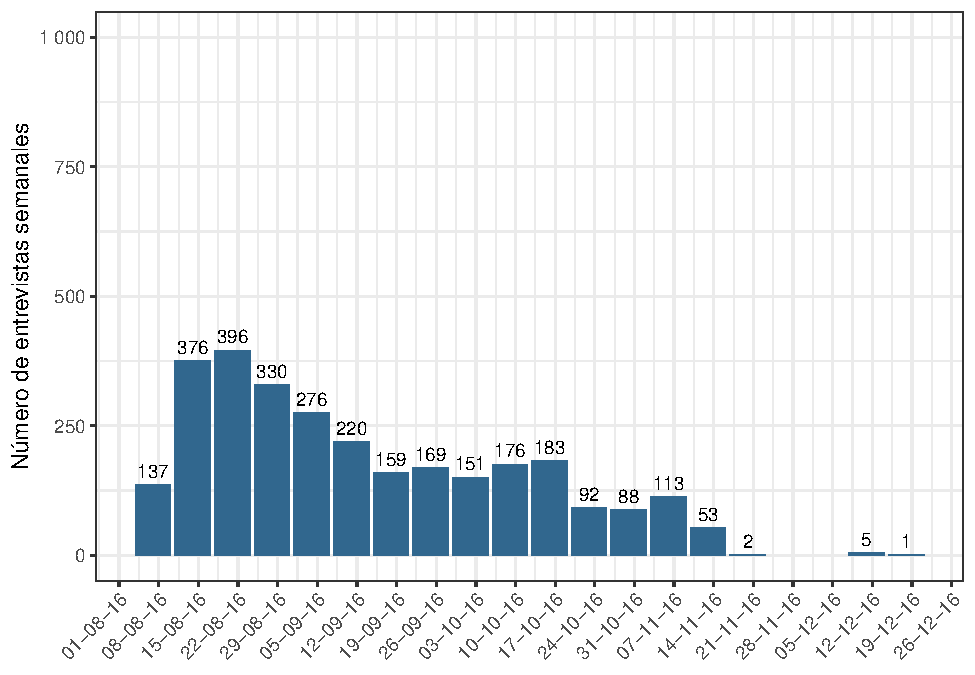
\includegraphics{manual-metodologico-elsoc_files/figure-latex/graf-fechas-ola1-1} 

}

\caption{Número de entrevistas por semana, ola 2016}\label{fig:graf-fechas-ola1}
\end{figure}

\hypertarget{indicadores-levantamiento}{%
\paragraph*{Indicadores levantamiento}\label{indicadores-levantamiento}}
\addcontentsline{toc}{paragraph}{Indicadores levantamiento}

A continuación se presentan las Tasas de Respuesta 1 (TRR1, definida por la AAPOR), Tasa de Cooperación 1 (TCC1), Tasa de Rechazo 1 (TR1) y Tasa de Contacto 1 (TC1)\footnote{Para mayor información sobre la determinación de los códigos de disposición final de casos y el cálculo de las tasas de resultados, ver
  \href{http://www.aapor.org/AAPOR_Main/media/publications/Standard-Definitions20169theditionfinal.pdf}{AAPOR (2016). Standard Definitions. Final Dispositions of Case Codes and Outcome Rates for Surveys}}

\begin{table}[H]

\caption{\label{tab:tabla-tasas-ola1}Tasas de Respuesta, Cooperación, de Rechazo y de Contacto, ola 2016}
\centering
\begin{tabular}[t]{lc}
\toprule
Indicador & Muestra Original\\
\midrule
Tasa de contacto & 72.6\%\\
Tasa de cooperación & 86.0\%\\
Tasa de rechazo & 8.9\%\\
Tasa de respuesta & 62.4\%\\
\bottomrule
\end{tabular}
\end{table}

\hypertarget{casos-falsificados}{%
\paragraph*{Corrección de datos por casos anómalos: Olas 2016 y 2017}\label{casos-falsificados}}
\addcontentsline{toc}{paragraph}{Corrección de datos por casos anómalos: Olas 2016 y 2017}

En el contexto de la ejecución de la tercera ola del estudio ELSOC (año 2018) se diagnosticó la falsificación de un número acotado de casos a lo largo del estudio en las olas 2016 y 2017.

Durante la etapa de supervisión del trabajo de encuestadores durante el 2018, tercera ola de ELSOC, el Centro de Microdatos (CMD) detectó e informó que un conjunto de casos incluidos en la muestra panel son falsos.

Debido al lento avance de las metas de campo de ELSOC en 2018 en Tarapacá y Valparaíso, se enviaron nuevos encuestadores, los cuales detectaron estos problemas. En específico, las encuestas fueron sistemáticamente falsificadas: se realizaron a otras personas no incluídas en la muestra, o los encuestadores solicitaron información a terceros.

Esto llevó a un proceso exhaustivo de revisión, en la cual se detectaron 56 casos falsificados en el campo de 2016 y 47 en el campo de 2017, concentrados en las regiones de Tarapacá (11 casos en 2016 y 11 en 2017) y Valparaíso (45 casos en 2016 y 37 en 2017).

La estrategia de campo de CMD se centra en encuestadores experimentados, asignando los mismos casos a los encuestadores en el tiempo, acorde a la recomendación de la literatura especializada. El problema se concentró en algunos encuestadores específicos en dichas zonas, el cual no fue detectado durante la supervisión de campo de las dos primeras olas.

Los casos falsificados representan el 1,9\% del tamaño muestral efectivo de ELSOC 2016 (N = 2.984) y 1,9\% de 2017 (N = 2.522), por lo que se considera que éstos tienen un impacto marginal a nivel general. A pesar de esto, se tomó la decisión de excluir de las bases de datos los casos falsificados, y se generó y puso a disposición una versión corregida de las bases de datos 2016 y 2017. Los ponderadores fueron corregidos considerando la eliminación de estos casos.

Para evitar estos problemas en el futuro, se modificaron los protocolos de supervisión, aumentando la supervisión presencial y el porcentaje de casos supervisados por encuestador. Adicionalmente, se implementó un sistema de rotación de encuestadores de tal manera que la muestra no sea levantada por los mismos encuestadores en más de una ronda.

\hypertarget{implementaciuxf3n-ola-2017}{%
\subsubsection{Implementación Ola 2017}\label{implementaciuxf3n-ola-2017}}

El levantamiento definitivo de la encuesta se llevó a cabo en un período de doce semanas, durante los meses de julio y octubre de 2017 (ver Figura \ref{fig:graf-fechas-ola2}). Para la ejecución del terreno se contó con 120 encuestadores distribuidos en las 17 sedes de trabajo.

El terreno se llevó a cabo en un período mayor al pronosticado, pues se estimó que duraría nueve semanas, extendiéndose finalmente a doce. Sin embargo, el levantamiento de datos tuvo una duración menor al de la primera ola, que se extendió por 20 semanas. Esta mayor rapidez fue propiciada por la disponibilidad de datos de contacto de los encuestados obtenido en la ola anterior.

La extensión del terreno por sobre la estimación original se debió principalmente a que en las regiones Metropolitana y de Valparaíso existió una mayor dificultad para contactar a los encuestados.

El cierre definitivo del trabajo de campo del levantamiento de la encuesta se desarrolló una vez cubierta la totalidad de la muestra. El terreno se cerró finalmente con 2.521 encuestas realizadas.

\begin{figure}

{\centering 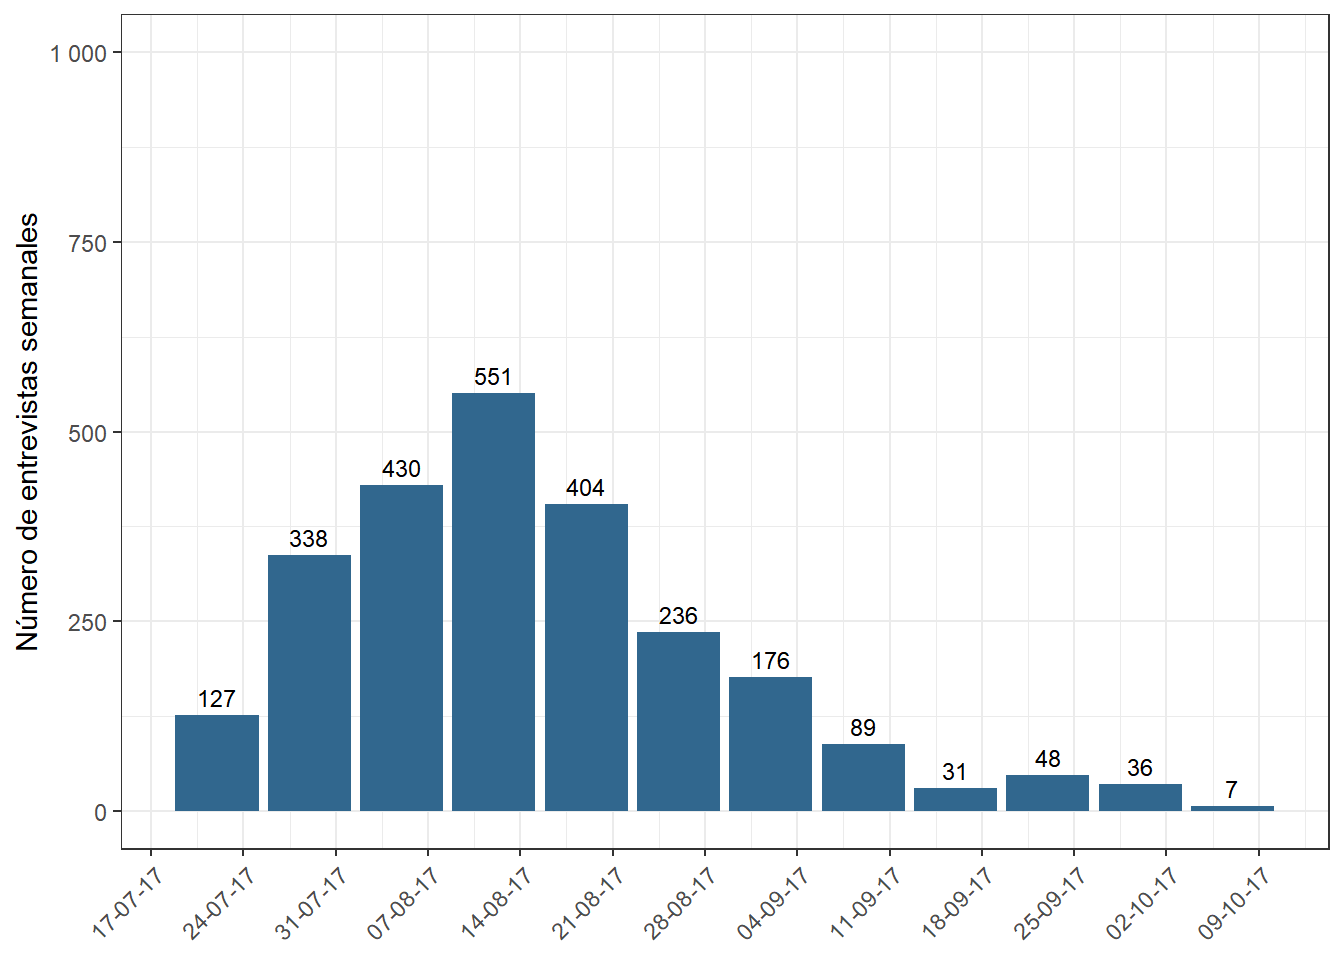
\includegraphics{manual-metodologico-elsoc_files/figure-latex/graf-fechas-ola2-1} 

}

\caption{Número de entrevistas por semana, ola 2017}\label{fig:graf-fechas-ola2}
\end{figure}

\hypertarget{indicadores-levantamiento-1}{%
\paragraph*{Indicadores levantamiento}\label{indicadores-levantamiento-1}}
\addcontentsline{toc}{paragraph}{Indicadores levantamiento}

A continuación se presentan las Tasas de Respuesta 1 (TRR1, definida por la AAPOR), Tasa de Cooperación 1 (TCC1), Tasa de Rechazo 1 (TR1) y Tasa de Contacto 1 (TC1):

\begin{table}[H]

\caption{\label{tab:tabla-tasas-ola2}Tasas de Respuesta, Cooperación, de Rechazo y de Contacto, ola 2017}
\centering
\begin{tabular}[t]{lc}
\toprule
Indicador & Muestra Original\\
\midrule
Tasa de contacto & 88.7\%\\
Tasa de cooperación & 93.1\%\\
Tasa de rechazo & 6.0\%\\
Tasa de respuesta & 82.6\%\\
\bottomrule
\end{tabular}
\end{table}

\hypertarget{casos-falsificados-en-ola-2017}{%
\paragraph{Casos falsificados en ola 2017}\label{casos-falsificados-en-ola-2017}}

Luego de los registros y procedimientos aplicados por el CMD el año 2018 se encontraron y corrigieron anomalías en encuestas realizadas en 2016 y 2017. Para más detalle del problema encontrado y su corrección revisar \protect\hyperlink{casos-falsificados}{Corrección de datos por casos falsificados: Olas 2016 y 2017}.

\hypertarget{implementaciuxf3n-ola-2018}{%
\subsubsection{Implementación Ola 2018}\label{implementaciuxf3n-ola-2018}}

El trabajo de terreno se desarrolló durante los meses de agosto a diciembre de 2018, dentro del tiempo estimado (15 semanas, aproximadamente) (ver Figura \ref{fig:graf-fechas-ola3}). Para la ejecución del terreno se contó con 189 encuestadores distribuidos en 18 sedes de trabajo.

Durante este levantamiento se incluyó la muestra de Refresco, lo que generó una dificultad para los encuestadores, ya que éstos deben explicar y motivar la participación en el estudio, tanto al grupo familiar como a los propios entrevistados.

Por otra parte, la muestra de seguimiento (muestra Original) de los entrevistados 2016-2017 tuvo dificultades de contactabilidad, debido a una mayor presencia de cambios de domicilios registrados que en las versiones anteriores de la encuesta. El 6,9\% se había cambiado a un domicilio diferente.

Otra de las dificultades enfrentadas en ola tiene relación con los casos de falsificación detectados (ver \protect\hyperlink{casos-falsificados}{Corrección de datos por casos falsificados: Olas 2016 y 2017}). Este problema implicó una revisión exhaustiva en terreno de estos casos, y un fortalecimiento al sistema de control, contemplando lo siguiente:

\begin{enumerate}
\def\labelenumi{\arabic{enumi}.}
\item
  Aumentar el porcentaje de encuestas a controlar, de 10\% a un 15\% el 2018. Asegurando controlar al menos el 20\% del trabajo realizado por cada encuestador.
\item
  Estipular para futuras olas del proyecto rotación de los encuestadores sobre el mismo entrevistado.
\item
  Registro de las encuestadoras involucradas de manera de no ser consideradas en futuras
  aplicaciones del estudio. Respecto a la dinámica general del trabajo, se crearon incentivos económicos para que los encuestadores lograran la muestra esperada. Así mismo, se dispuso la movilización necesaria para que los encuestadores cubrieran toda la muestra en los distintos horarios.
\end{enumerate}

El cierre definitivo del trabajo de campo del levantamiento de la encuesta se desarrolló de común acuerdo con COES, una vez cubierta la totalidad de la muestra. El terreno se cerró con 2.274 encuestas en la muestra de seguimiento y 1.523 encuestas en la muestra de refresco.

\begin{figure}

{\centering 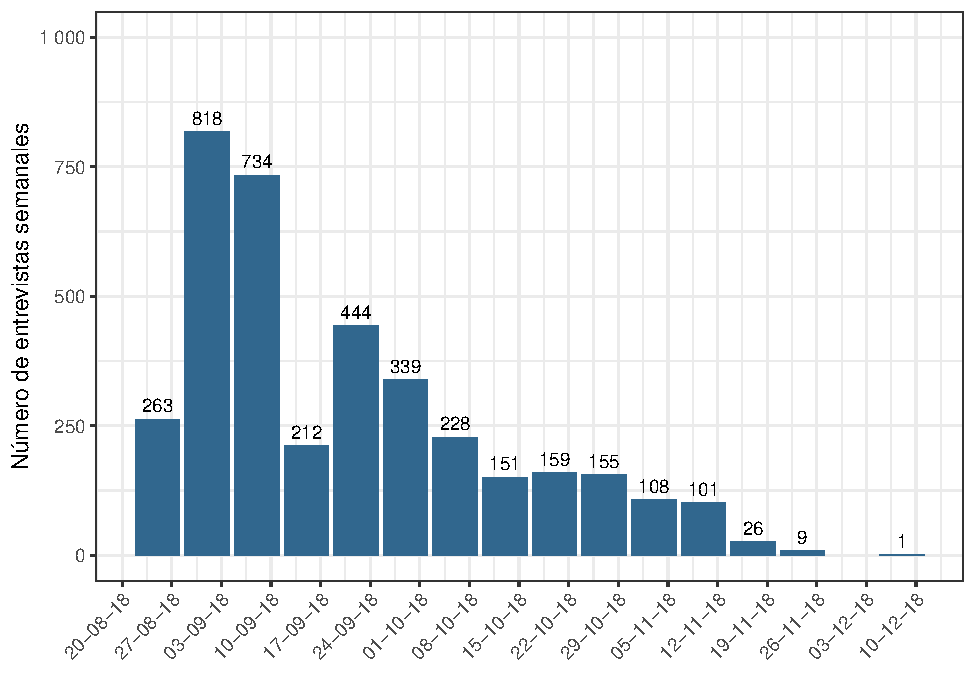
\includegraphics{manual-metodologico-elsoc_files/figure-latex/graf-fechas-ola3-1} 

}

\caption{Número de entrevistas por semana, ola 2018}\label{fig:graf-fechas-ola3}
\end{figure}

\hypertarget{indicadores-levantamiento-2}{%
\paragraph*{Indicadores levantamiento}\label{indicadores-levantamiento-2}}
\addcontentsline{toc}{paragraph}{Indicadores levantamiento}

A continuación se presentan las Tasas de Respuesta 1 (TRR1, definida por la AAPOR), Tasa de Cooperación 1 (TCC1), Tasa de Rechazo 1 (TR1) y Tasa de Contacto 1 (TC1):

\begin{table}[H]

\caption{\label{tab:tabla-tasas-ola3}Tasas de Respuesta, Cooperación, de Rechazo y de Contacto, ola 2018}
\centering
\begin{tabular}[t]{lcc}
\toprule
Indicador & Muestra Original & Muestra Refresco\\
\midrule
Tasa de contacto & 86.0\% & 66.0\%\\
Tasa de cooperación & 93.0\% & 88.0\%\\
Tasa de rechazo & 5.0\% & 8.0\%\\
Tasa de respuesta & 80.0\% & 58.0\%\\
\bottomrule
\end{tabular}
\end{table}

\hypertarget{implementaciuxf3n-ola-2019}{%
\subsubsection{Implementación Ola 2019}\label{implementaciuxf3n-ola-2019}}

El levantamiento de datos de ELSOC 2019 estaba programado para comenzar el sábado 19 de octubre de 2019, sin embargo debido al Estallido Social ocurrido en Chile a partir del 18 de octubre de 2019, el trabajo de terreno debió ser suspendido hasta el jueves 21 de noviembre, fecha en que se inició finalmente la recolección de la información. Por lo tanto, el levantamiento se realizó durante el período de Estallido Social, lo que dificultó su ejecución.

Esta labor se extendió por un periodo de 13 semanas (Dado el desgaste propio de la muestra y del equipo de terreno, se decidió hacer una pausa en el levantamiento de datos durante las últimas 3 semanas de febrero de 2020) (ver Figura \ref{fig:graf-fechas-ola4}). Para la ejecución del terreno se contó con 143 encuestadores distribuidos en 16 sedes de trabajo, administradas por coordinadores de zona debidamente capacitados.

\begin{figure}

{\centering 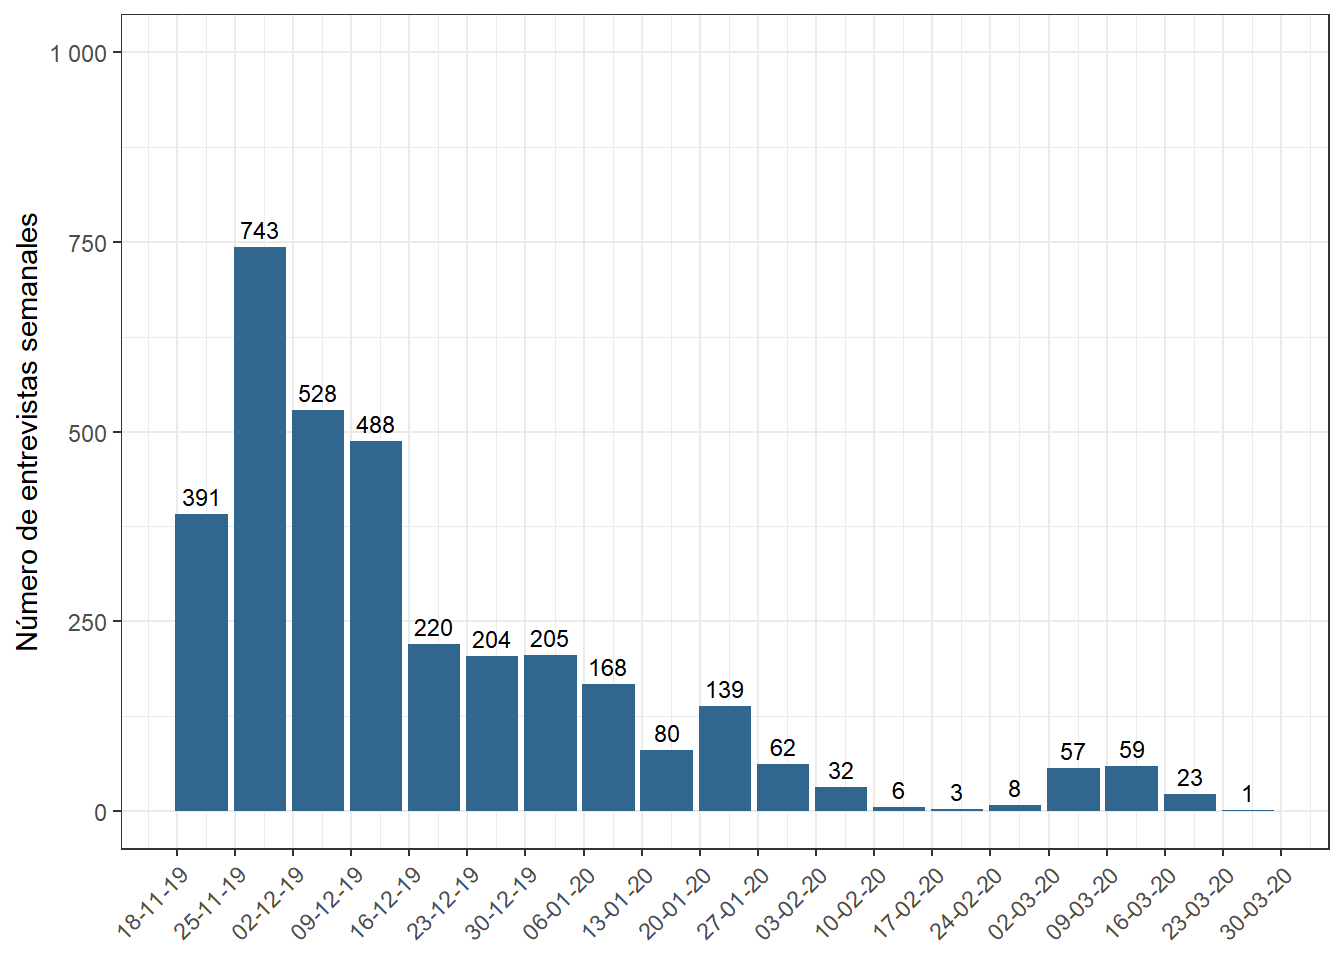
\includegraphics{manual-metodologico-elsoc_files/figure-latex/graf-fechas-ola4-1} 

}

\caption{Número de entrevistas por semana, ola 2019}\label{fig:graf-fechas-ola4}
\end{figure}

\hypertarget{indicadores-levantamiento-3}{%
\paragraph*{Indicadores levantamiento}\label{indicadores-levantamiento-3}}
\addcontentsline{toc}{paragraph}{Indicadores levantamiento}

A continuación se presentan las Tasas de Respuesta 1 (TRR1, definida por la AAPOR), Tasa de Cooperación 1 (TCC1), Tasa de Rechazo 1 (TR1) y Tasa de Contacto 1 (TC1):

\begin{table}[H]

\caption{\label{tab:tabla-tasas-ola4}Tasas de Respuesta, Cooperación, de Rechazo y de Contacto, ola 2019}
\centering
\begin{tabular}[t]{lcc}
\toprule
Indicador & Muestra Original & Muestra Refresco\\
\midrule
Tasa de contacto & 86.0\% & 87.0\%\\
Tasa de cooperación & 93.0\% & 95.0\%\\
Tasa de rechazo & 5.0\% & 3.0\%\\
Tasa de respuesta & 80.0\% & 83.0\%\\
\bottomrule
\end{tabular}
\end{table}

\hypertarget{implementaciuxf3n-ola-2021}{%
\subsubsection{Implementación Ola 2021}\label{implementaciuxf3n-ola-2021}}

La crisis sanitaria producida por la pandemia de COVID-19 y las restricciones asociadas, implicaron cambiar la metodología de aplicación de la Encuesta Longitudinal Social de Chile de forma presencial a remota a través de una encuesta telefónica (Para más detalle ver \protect\hyperlink{instrumento-covid}{Cuestionario 2021: levantamiento durante la pandemia de COVID-19}). Este cambio en la forma de levantar los datos, presentó un gran desafío logístico y operativo, ya que desde sus orígenes ELSOC se había levantado de manera presencial.

La pandemia de COVID-19 también afectó la fecha tradicional de levantamiento de ELSOC, la cual estaba programada para comenzar durante octubre de 2020, sin embargo, el levantamiento de la quinta ola se inició el sábado 30 de enero de 2021 con la asignación de la muestra a los encuestadores capacitados. Las razones para postergar el período de levantamiento fueron principalmente por la espera de condiciones sanitarias y de cuarentenas más favorables que permitieran un levantamiento presencial (sin embargo, prontamente se volvió clara la imposibilidad de mantener la modalidad presencial); y por el tiempo adicional que tomó la preparación del terreno, producto del cambio de modalidad de levantamiento. El trabajo de campo se extendió hasta mediados de junio de 2021. Sin embargo, la aplicación se realizó mayoritariamente entre febrero y abril de 2021 (ver Figura \ref{fig:graf-fechas-ola5}).

Debido al degaste de la muestra y al desgaste del equipo de encuestadores por intentos infructuosos de contacto, es que a contar del mes de mayo se decidió cambiar la metodología de aplicación de producción por unidad muestral a conformar un grupo de encuestadores dedicado exclusivamente a repasar la muestra en una jornada laboral determinada.

\begin{figure}

{\centering 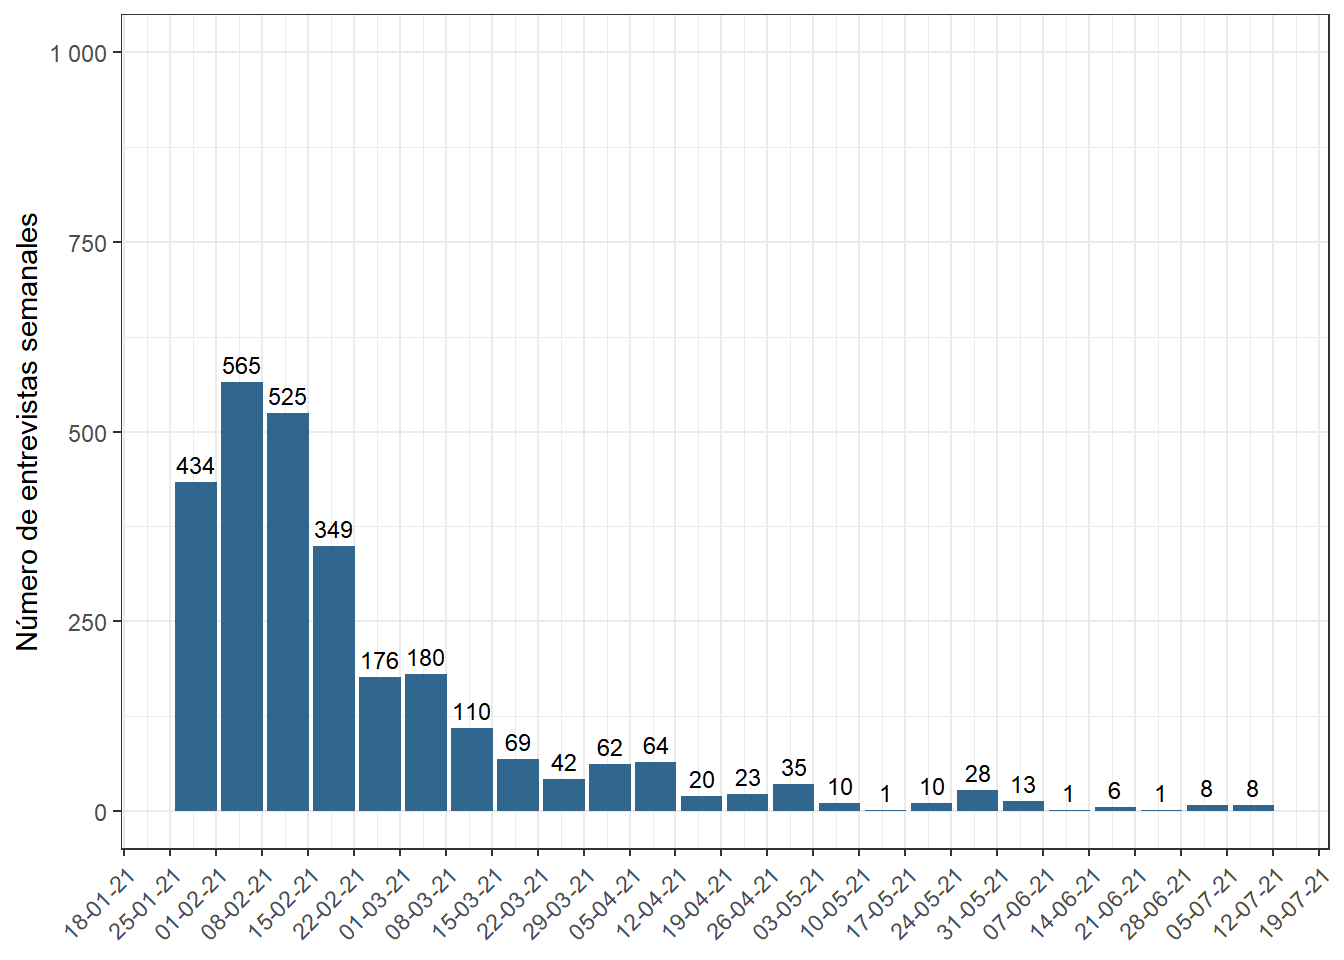
\includegraphics{manual-metodologico-elsoc_files/figure-latex/graf-fechas-ola5-1} 

}

\caption{Número de entrevistas por semana, ola 2021}\label{fig:graf-fechas-ola5}
\end{figure}

\hypertarget{indicadores-levantamiento-4}{%
\paragraph*{Indicadores levantamiento}\label{indicadores-levantamiento-4}}
\addcontentsline{toc}{paragraph}{Indicadores levantamiento}

A continuación se presentan las Tasas de Respuesta 1 (TRR1, definida por la AAPOR), Tasa de Cooperación 1 (TCC1), Tasa de Rechazo 1 (TR1) y Tasa de Contacto 1 (TC1):

\begin{table}[H]

\caption{\label{tab:tabla-tasas-ola5}Tasas de Respuesta, Cooperación, de Rechazo y de Contacto, ola 2021}
\centering
\begin{tabular}[t]{lcc}
\toprule
Indicador & Muestra Original & Muestra Refresco\\
\midrule
Tasa de contacto & 78.0\% & 87.3\%\\
Tasa de cooperación & 83.7\% & 76.1\%\\
Tasa de rechazo & 11.0\% & 8.8\%\\
Tasa de respuesta & 65.2\% & 66.5\%\\
\bottomrule
\end{tabular}
\end{table}

\hypertarget{atricion}{%
\subsection{Atrición de la encuesta}\label{atricion}}

A continuación, se presenta la atrición obtenida según Muestra:

\begin{table}[H]

\caption{\label{tab:tabla-atricion}Atrición de las muestras de ELSOC entre olas}
\centering
\begin{tabular}[t]{ccccc}
\toprule
\multicolumn{1}{c}{ } & \multicolumn{2}{c}{Muestra Lograda} & \multicolumn{2}{c}{Tasa de Atrición} \\
\cmidrule(l{3pt}r{3pt}){2-3} \cmidrule(l{3pt}r{3pt}){4-5}
Medición & Muestra Original & Muestra Refresco & Muestra Original & Muestra Refresco\\
\midrule
2016 & 2927 &  &  & \\
2017 & 2473 &  & 15.5\% & \\
2018 & 2229 & 1519 & 9.9\% & \\
2019 & 2153 & 1264 & 3.4\% & 16.8\%\\
2021 & 1739 & 1001 & 19.2\% & 20.8\%\\
\bottomrule
\end{tabular}
\end{table}

\begin{itemize}
\tightlist
\item
  Según sexo:
\end{itemize}

\begin{table}[H]

\caption{\label{tab:unnamed-chunk-2}Atrición de las muestras de ELSOC entre olas, según sexo}
\centering
\begin{tabular}[t]{ccccc}
\toprule
\multicolumn{1}{c}{ } & \multicolumn{2}{c}{Muestra Lograda} & \multicolumn{2}{c}{Tasa de Atrición} \\
\cmidrule(l{3pt}r{3pt}){2-3} \cmidrule(l{3pt}r{3pt}){4-5}
Medición & Hombres & Mujeres & Hombres & Mujeres\\
\midrule
\addlinespace[0.3em]
\multicolumn{5}{l}{\textbf{Muestra Original}}\\
\hspace{1em}2016 & 1163 & 1764 &  & \\
\hspace{1em}2017 & 953 & 1520 & 18.1\% & 13.8\%\\
\hspace{1em}2018 & 841 & 1387 & 11.8\% & 8.8\%\\
\hspace{1em}2019 & 807 & 1346 & 4.0\% & 3.0\%\\
\hspace{1em}2021 & 631 & 1108 & 21.8\% & 17.7\%\\
\addlinespace[0.3em]
\multicolumn{5}{l}{\textbf{Muestra Refresco}}\\
\hspace{1em}2018 & 607 & 912 &  & \\
\hspace{1em}2019 & 482 & 782 & 20.6\% & 14.3\%\\
\hspace{1em}2021 & 378 & 623 & 21.6\% & 20.3\%\\
\bottomrule
\end{tabular}
\end{table}

\begin{itemize}
\tightlist
\item
  Según tramo etareo:
\end{itemize}

\begin{table}[H]

\caption{\label{tab:unnamed-chunk-3}Atrición de las muestras de ELSOC entre olas, según tramo etáreo}
\centering
\begin{tabular}[t]{ccccccccc}
\toprule
\multicolumn{1}{c}{ } & \multicolumn{4}{c}{Muestra Lograda} & \multicolumn{4}{c}{Tasa de Atrición} \\
\cmidrule(l{3pt}r{3pt}){2-5} \cmidrule(l{3pt}r{3pt}){6-9}
Medición & 19-29 & 30-49 & 50-64 & 65 o más & 19-29 & 30-49 & 50-64 & 65 o más\\
\midrule
\addlinespace[0.3em]
\multicolumn{9}{l}{\textbf{Muestra Original}}\\
\hspace{1em}2016 & 506 & 1157 & 839 & 425 &  &  &  & \\
\hspace{1em}2017 & 407 & 962 & 734 & 370 & 19.6\% & 16.9\% & 12.5\% & 12.9\%\\
\hspace{1em}2018 & 340 & 863 & 687 & 338 & 16.5\% & 10.3\% & 6.4\% & 8.6\%\\
\hspace{1em}2019 & 327 & 838 & 666 & 322 & 3.8\% & 2.9\% & 3.1\% & 4.7\%\\
\hspace{1em}2021 & 269 & 685 & 546 & 239 & 17.7\% & 18.3\% & 18.0\% & 25.8\%\\
\addlinespace[0.3em]
\multicolumn{9}{l}{\textbf{Muestra Refresco}}\\
\hspace{1em}2018 & 341 & 579 & 418 & 181 &  &  &  & \\
\hspace{1em}2019 & 271 & 472 & 369 & 152 & 20.5\% & 18.5\% & 11.7\% & 16.0\%\\
\hspace{1em}2021 & 216 & 391 & 282 & 112 & 20.3\% & 17.2\% & 23.6\% & 26.3\%\\
\bottomrule
\end{tabular}
\end{table}

\begin{itemize}
\tightlist
\item
  Según nivel educacional:
\end{itemize}

\begin{table}[H]

\caption{\label{tab:unnamed-chunk-4}Atrición de las muestras de ELSOC entre olas, según nivel educacional}
\centering
\begin{tabular}[t]{ccccccccc}
\toprule
\multicolumn{1}{c}{ } & \multicolumn{4}{c}{Muestra Lograda} & \multicolumn{4}{c}{Tasa de Atrición} \\
\cmidrule(l{3pt}r{3pt}){2-5} \cmidrule(l{3pt}r{3pt}){6-9}
Medición & Básica & Media & Técnica & Universitaria & Básica & Media & Técnica & Universitaria\\
\midrule
\addlinespace[0.3em]
\multicolumn{9}{l}{\textbf{Muestra Original}}\\
\hspace{1em}2016 & 656 & 1251 & 483 & 535 &  &  &  & \\
\hspace{1em}2017 & 580 & 1062 & 396 & 434 & 11.6\% & 15.1\% & 18.0\% & 18.9\%\\
\hspace{1em}2018 & 512 & 977 & 358 & 380 & 11.7\% & 8.0\% & 9.6\% & 12.4\%\\
\hspace{1em}2019 & 490 & 953 & 341 & 368 & 4.3\% & 2.5\% & 4.7\% & 3.2\%\\
\hspace{1em}2021 & 363 & 757 & 283 & 336 & 25.9\% & 20.6\% & 17.0\% & 8.7\%\\
\addlinespace[0.3em]
\multicolumn{9}{l}{\textbf{Muestra Refresco}}\\
\hspace{1em}2018 & 283 & 633 & 253 & 347 &  &  &  & \\
\hspace{1em}2019 & 254 & 537 & 206 & 264 & 10.2\% & 15.2\% & 18.6\% & 23.9\%\\
\hspace{1em}2021 & 167 & 426 & 175 & 233 & 34.3\% & 20.7\% & 15.0\% & 11.7\%\\
\bottomrule
\end{tabular}
\end{table}

\newpage

\hypertarget{bases-datos}{%
\section{Bases de Datos}\label{bases-datos}}

\hypertarget{descarga-de-bases-de-datos}{%
\subsection{Descarga de Bases de datos}\label{descarga-de-bases-de-datos}}

Las bases de datos ELSOC son puestas a disposición al público general en el momento en que se ha completado su proceso de revisión y validación. Las bases de datos son publicadas y archivadas en el repositorio de \textbf{Harvard Dataverse}, en la \href{https://dataverse.harvard.edu/dataverse/coes_data_repository}{carpeta de datos de COES}. Este repositorio permite un acceso gratuito y seguro a las bases de datos.

ELSOC se pone a disposición como bases de datos transversales según ola: olas 2016, 2017, 2018, 2019 y 2021, en formato de datos de R (.RData), SPSS (.sav), Stata 13 (.dta) y Stata 14 (.dta).

Adicionalmente, a partir de 2019, se publican las bases de datos en formato longitudinal, para facilitar su uso como encuesta panel. A la fecha se encuentran publicadas la base longitudinal de olas 2016-2019 en formato wide, y bases longitudinal de olas 2016-2021 en formato wide y long. Las variables que han presentado cambios en el tiempo se encuentran armonizadas para permitir su uso longitudinal.

Como parte de un proceso continuo de mejora, es posible que las bases de datos publicadas sean actualizadas durante el desarrollo de ELSOC, debido a la corrección de potenciales errores, mejoras en el formato de los datos, actualización de códigos de no respuesta, etc. Dado esto, en el repositorio de Harvard Dataverse se encuentra publicada la última versión disponible, así como todas las versiones anteriores en caso de ser necesarias.

\hypertarget{fichas-tuxe9cnicas}{%
\subsection{Fichas Técnicas}\label{fichas-tuxe9cnicas}}

En este apartado se presenta la Ficha Técnica (Ver Cuadro \ref{tab:ficha}, dónde se sintetizan las principales características del Estudio Longitudinal Social de Chile (ELSOC COES):

\begin{table}[H]

\caption{\label{tab:ficha}Ficha Técnica ELSOC COES}
\centering
\resizebox{\linewidth}{!}{
\begin{tabular}[t]{>{\raggedright\arraybackslash}p{7em}>{\raggedright\arraybackslash}p{35em}}
\toprule
Características & ELSOC\\
\midrule
Objetivo & Analizar longitudinalmente la evolución del conflicto y cohesión
                              en la sociedad chilena\\
Diseño & Estudio cuantitativo por medio de un cuestionario estructurado\\
Instrumento & Cuestionario compuesto por preguntas cerradas de carácter simple y múltiple junto a algunas preguntas abiertas\\
Unidad de análisis & Individuos\\
Población objetivo & Hombres y mujeres de 18 a 75 años, residentes habituales de viviendas particulares\\
\addlinespace
Marco muestral & Marco de muestreo de manzanas del pre-censo 2011, trabajo elaborado por el Centro de Inteligencia Territorial (CIT) de la Universidad Adolfo Ibáñez\\
Diseño muestral & Probabilístico, estratificado, por conglomerados y multietápico\\
Unidades de muestreo & Primero se eligen ciudades (UPM), luego manzanas (USM), y sub-bloques y viviendas (UTM). La unidad final de selección es la persona\\
Periodicidad & Anual. Muestra de refresco a oartir del 3er año\\
Modo de aplicación & Formato CAPI en vivienda del entrevistado. Formato CATI durante 2021\\
\addlinespace
Informante & Hombre o mujer residente en la vivienda, con edad entre 18 y 75 años.\\
Duración promedio & 51 minutos\\
Representatividad & Aproximadamente el 77\% de la población total del país y 93\% de la
              población urbana con la muestra de Ola 2016\\
Organismo responsable & Centro de Estudios del Conflicto y Cohesión Social (COES)\\
Organismo ejecutor & CentroMicroDatos (CMD) de la Universidad de Chile\\
\bottomrule
\end{tabular}}
\end{table}

\hypertarget{protocolo-de-uso-de-base-de-datos}{%
\subsection{Protocolo de Uso de Base de Datos}\label{protocolo-de-uso-de-base-de-datos}}

Cualquier publicación que utilize las bases de datos ELSOC, en cualquiera de sus versiones, debe citar la fuente de las siguientes formas (dependiendo de la base utilizada):

\begin{itemize}
\tightlist
\item
  ELSOC 2016:
\end{itemize}

\textbf{Centro de Estudios de Conflicto y Cohesión Social (2016). Estudio Longitudinal Social de Chile, Primera Ola (ELSOC\_W01\_v1.00). {[}Archivo de datos{]}. Santiago, Chile: Centro de Estudios de Conflicto y Cohesión Social (COES). www.coes.cl}

\begin{itemize}
\tightlist
\item
  ELSOC 2017:
\end{itemize}

\textbf{Centro de Estudios de Conflicto y Cohesión Social (2017). Estudio Longitudinal Social de Chile, Segunda Ola (ELSOC\_W02\_v1.00). {[}Archivo de datos{]}. Santiago, Chile: Centro de Estudios de Conflicto y Cohesión Social (COES). www.coes.cl}

\begin{itemize}
\tightlist
\item
  ELSOC 2018:
\end{itemize}

\textbf{Centro de Estudios de Conflicto y Cohesión Social (2018). Estudio Longitudinal Social de Chile, Tercera Ola (ELSOC\_W03\_v1.00). {[}Archivo de datos{]}. Santiago, Chile: Centro de Estudios de Conflicto y Cohesión Social (COES). www.coes.cl}

\begin{itemize}
\tightlist
\item
  ELSOC 2019:
\end{itemize}

\textbf{Centro de Estudios de Conflicto y Cohesión Social (2019). Estudio Longitudinal Social de Chile, Cuarta Ola (ELSOC\_W04\_v1.00). {[}Archivo de datos{]}. Santiago, Chile: Centro de Estudios de Conflicto y Cohesión Social (COES). www.coes.cl}

\begin{itemize}
\tightlist
\item
  ELSOC 2021:
\end{itemize}

\textbf{Centro de Estudios de Conflicto y Cohesión Social (2021). Estudio Longitudinal Social de Chile, Quinta Ola (ELSOC\_W05\_v1.00). {[}Archivo de datos{]}. Santiago, Chile: Centro de Estudios de Conflicto y Cohesión Social (COES). www.coes.cl}

O en su formato longitudinal:

\textbf{Centro de Estudios de Conflicto y Cohesión Social (2021). Estudio Longitudinal Social de Chile, Versión Panel Combinada 2016-2019 (ELSOC\_Wide\_2016\_2019\_v1.00). {[}Archivo de datos{]}. Santiago, Chile: Centro de Estudios de Conflicto y Cohesión Social (COES). www.coes.cl}

Por último, en caso de que se desee citar el presente Manual de Usuario:

**Centro de Estudios de Conflicto y Cohesión Social (2021). Manual de Usuario de Estudio Longitudinal Social de Chile. Santiago, Chile: Centro de Estudios de Conflicto y Cohesión Social (COES).*

**

Centro de Estudios de Conflicto y Cohesión Social (2021). Estudio Longitudinal Social de Chile, Quinta Ola (ELSOC\_W05\_v1.00). {[}Archivo de datos{]}. Santiago, Chile: Centro de Estudios de Conflicto y Cohesión Social (COES). www.coes.cl

\newpage

\hypertarget{libro-codigos}{%
\section{Libro de Códigos}\label{libro-codigos}}

Para un uso adecuado de la base de datos de ELSOC COES se recomienda a los investigadores trabajar con el libro de códigos, el cual se presenta a continuación. Este apartado detalla el codigo longitudinal de cada variable; la etiqueta de variable asociada; fraseo de cada preambulo, pregunta e item; las distintas categorías de respuestas y codigos asociados; y observaciones en las variables que han tenido modificaciones a lo largo de las distintas mediciones del estudio. Adicionalmente, se incluyen tablas de frecuencia de cada pregunta según ola y muestra (se omiten variables numéricas continuas y de texto).

El libro de códigos fue diseñado de modo de que sintetice toda la información relevante sobre las variables de la base de datos en un formato común para facilitar su uso. De manera genérica, las variables incluidas en la base de datos tienen el siguiente formato:

\begin{quote}
\textbf{Código longitudinal}. Etiqueta de variable

\emph{Fraseo pregunta}

\emph{Códigos de respuestas Categorías de respuesta}

Observaciones

Tabla de frecuencias
\end{quote}

Las preguntas se presentan por módulo del cuestionario, para facilitar su lectura.

El Código Longitudinal corresponde al código asociado a cada item del cuestionario en la base de datos y libros de códigos. Por medio de estos códigos se pueden identificar los distintos ítemes incluidos. En el caso de la base de datos longitudinal en formato Wide, el código incluye *\_w01\emph{, }\_w02\emph{, }\_w03\emph{, }\_w04* o *\_w05* al final del código para indicar si la respuesta corresponde a las olas 2016, 2017, 2018, 2019 o 221, respectivamente.

Las etiquetas de variables se incluyen en el Libro de Códigos y en las bases de datos, y fueron diseñadas por el equipo ELSOC con el objetivo de describir de modo sucinto el fenómeno o dimensión a medir\footnote{Se eliminan tildes y otros símbolos no incluidos en todos los softwares estadísticos (por ejemplo, tildes y la ñ)}. A continuación se presenta el fraseo de la pregunta, incluyendo los preámbulos, y los distintos códigos y categorías de respuesta. En la construcción de la base de datos, los códigos de respuesta fueron ingresados como valores numéricos y las categorías de respuesta como etiquetas de valores.

Finalmente, se incorporan observaciones asociadas a posibles cambios en el tiempo, o aspectos a tomar en consideración al momento de utilizar las variables.

Las variables de cadena (texto) no presentan códigos, ya que presentan los verbatim literales de las menciones por parte de los encuestados. En el caso de los ítems dónde se pide una respuesta numérica tampoco existen categorías de respuesta, registrándose el valor indicado por el entrevistado.

\hypertarget{muxf3dulo-de-ciudadanuxeda-y-democracia}{%
\subsection{Módulo de Ciudadanía y democracia}\label{muxf3dulo-de-ciudadanuxeda-y-democracia}}

\begin{itemize}
\tightlist
\item
  \textbf{c01}: Satisfaccion con la democracia en Chile
\end{itemize}

\begin{quote}
\emph{¿Cuán satisfecho o insatisfecho está usted con el funcionamiento de la democracia en Chile?}.
\end{quote}

\begin{quote}
-999 No Responde (no leer)\\
-888 No Sabe (no leer)\\
-777 Valor perdido por error tecnico\\
-666 Valor perdido por encuesta incompleta\\
1 Nada satisfecho\\
2 Poco satisfecho\\
3 Algo satisfecho\\
4 Bastante satisfecho\\
5 Muy satisfecho
\end{quote}

\begin{table}[H]
\begin{tabular}[t]{lccccc}
\toprule
c01 & 2016 & 2017 & 2018 & 2019 & 2021\\
\midrule
\addlinespace[0.3em]
\multicolumn{6}{l}{\textbf{Muestra Original}}\\
\hspace{1em}-999 & 22 & 20 & 16 & 14 & 5\\
\hspace{1em}-888 & 107 & 98 & 102 & 46 & 18\\
\hspace{1em}-666 & 0 & 0 & 0 & 0 & 0\\
\hspace{1em}1 & 1228 & 866 & 616 & 1117 & 553\\
\hspace{1em}2 & 704 & 651 & 598 & 587 & 606\\
\hspace{1em}3 & 591 & 558 & 619 & 282 & 446\\
\hspace{1em}4 & 202 & 231 & 234 & 78 & 94\\
\hspace{1em}5 & 73 & 49 & 44 & 29 & 17\\
\addlinespace[0.3em]
\multicolumn{6}{l}{\textbf{Muestra Refresco}}\\
\hspace{1em}-999 & 0 & 0 & 17 & 6 & 3\\
\hspace{1em}-888 & 0 & 0 & 72 & 32 & 10\\
\hspace{1em}-666 & 0 & 0 & 0 & 0 & 8\\
\hspace{1em}1 & 0 & 0 & 446 & 669 & 295\\
\hspace{1em}2 & 0 & 0 & 438 & 329 & 373\\
\hspace{1em}3 & 0 & 0 & 361 & 181 & 236\\
\hspace{1em}4 & 0 & 0 & 147 & 31 & 64\\
\hspace{1em}5 & 0 & 0 & 38 & 16 & 12\\
\bottomrule
\end{tabular}
\end{table}

\begin{itemize}
\tightlist
\item
  \textbf{c02}: Confianza Social Generalizada
\end{itemize}

\begin{quote}
\emph{Hablando en general, ¿diría usted que se puede confiar en la mayoría de las personas, o que hay que tener cuidado al tratar con ellas?}.
\end{quote}

\begin{quote}
-999 No Responde (no leer)\\
-888 No Sabe (no leer)\\
-777 Valor perdido por error tecnico\\
-666 Valor perdido por encuesta incompleta\\
1 Casi siempre se puede confiar en las personas\\
2 Casi siempre hay que tener cuidado al tratar con las personas\\
3 Depende (no leer)
\end{quote}

\begin{table}[H]
\begin{tabular}[t]{lccccc}
\toprule
c02 & 2016 & 2017 & 2018 & 2019 & 2021\\
\midrule
\addlinespace[0.3em]
\multicolumn{6}{l}{\textbf{Muestra Original}}\\
\hspace{1em}-999 & 12 & 2 & 5 & 0 & 0\\
\hspace{1em}-888 & 34 & 30 & 7 & 2 & 0\\
\hspace{1em}-666 & 0 & 0 & 0 & 0 & 0\\
\hspace{1em}1 & 276 & 272 & 231 & 214 & 131\\
\hspace{1em}2 & 2373 & 1987 & 1840 & 1850 & 1579\\
\hspace{1em}3 & 232 & 182 & 146 & 87 & 29\\
\addlinespace[0.3em]
\multicolumn{6}{l}{\textbf{Muestra Refresco}}\\
\hspace{1em}-999 & 0 & 0 & 3 & 0 & 0\\
\hspace{1em}-888 & 0 & 0 & 10 & 2 & 1\\
\hspace{1em}-666 & 0 & 0 & 0 & 0 & 8\\
\hspace{1em}1 & 0 & 0 & 156 & 109 & 75\\
\hspace{1em}2 & 0 & 0 & 1256 & 1091 & 880\\
\hspace{1em}3 & 0 & 0 & 94 & 62 & 37\\
\bottomrule
\end{tabular}
\end{table}

\begin{itemize}
\tightlist
\item
  \textbf{c03}: Altruismo Social Generalizado
\end{itemize}

\begin{quote}
\emph{¿Diría usted que las personas, la mayoría de las veces, tratan de ayudar a los demás, o se preocupan mayormente sólo de Si mismas?}.
\end{quote}

\begin{quote}
-999 No Responde (no leer)\\
-888 No Sabe (no leer)\\
-777 Valor perdido por error tecnico\\
-666 Valor perdido por encuesta incompleta\\
1 La mayoria de las veces tratan de ayudar a los demas\\
2 La mayoria de las veces se preocupan solo de si mismas\\
3 Depende (no leer)
\end{quote}

\begin{table}[H]
\begin{tabular}[t]{lccccc}
\toprule
c03 & 2016 & 2017 & 2018 & 2019 & 2021\\
\midrule
\addlinespace[0.3em]
\multicolumn{6}{l}{\textbf{Muestra Original}}\\
\hspace{1em}-999 & 9 & 2 & 4 & 0 & 0\\
\hspace{1em}-888 & 24 & 21 & 11 & 5 & 3\\
\hspace{1em}-666 & 0 & 0 & 0 & 0 & 0\\
\hspace{1em}1 & 414 & 472 & 390 & 413 & 324\\
\hspace{1em}2 & 2196 & 1753 & 1611 & 1611 & 1302\\
\hspace{1em}3 & 284 & 225 & 213 & 124 & 110\\
\addlinespace[0.3em]
\multicolumn{6}{l}{\textbf{Muestra Refresco}}\\
\hspace{1em}-999 & 0 & 0 & 1 & 0 & 0\\
\hspace{1em}-888 & 0 & 0 & 8 & 3 & 2\\
\hspace{1em}-666 & 0 & 0 & 0 & 0 & 8\\
\hspace{1em}1 & 0 & 0 & 240 & 269 & 177\\
\hspace{1em}2 & 0 & 0 & 1128 & 913 & 739\\
\hspace{1em}3 & 0 & 0 & 142 & 79 & 75\\
\bottomrule
\end{tabular}
\end{table}

\begin{itemize}
\tightlist
\item
  \textbf{c04}: Mayoria de la gente trata de ser justa
\end{itemize}

\begin{quote}
\emph{¿Cree que la mayoría de la gente intentaría aprovecharse de usted si tuviera la oportunidad, o cree que trataría de ser justa?}.
\end{quote}

\begin{quote}
-999 No Responde (no leer)\\
-888 No Sabe (no leer)\\
-777 Valor perdido por error tecnico\\
-666 Valor perdido por encuesta incompleta\\
1 La mayoria de la gente intentaria aprovecharse\\
2 La mayoria de la gente trataria de ser justa\\
3 Depende (no leer)
\end{quote}

\begin{table}[H]
\begin{tabular}[t]{lccccc}
\toprule
c04 & 2016 & 2017 & 2018 & 2019 & 2021\\
\midrule
\addlinespace[0.3em]
\multicolumn{6}{l}{\textbf{Muestra Original}}\\
\hspace{1em}-999 & 14 & 3 & 4 & 1 & 1\\
\hspace{1em}-888 & 44 & 36 & 27 & 27 & 10\\
\hspace{1em}-666 & 0 & 0 & 0 & 0 & 0\\
\hspace{1em}1 & 1797 & 1350 & 1287 & 1286 & 1107\\
\hspace{1em}2 & 723 & 787 & 641 & 653 & 513\\
\hspace{1em}3 & 349 & 297 & 270 & 186 & 108\\
\addlinespace[0.3em]
\multicolumn{6}{l}{\textbf{Muestra Refresco}}\\
\hspace{1em}-999 & 0 & 0 & 5 & 1 & 0\\
\hspace{1em}-888 & 0 & 0 & 17 & 12 & 9\\
\hspace{1em}-666 & 0 & 0 & 0 & 0 & 8\\
\hspace{1em}1 & 0 & 0 & 899 & 717 & 606\\
\hspace{1em}2 & 0 & 0 & 420 & 407 & 311\\
\hspace{1em}3 & 0 & 0 & 178 & 127 & 67\\
\bottomrule
\end{tabular}
\end{table}

\begin{itemize}
\tightlist
\item
  \textbf{c05\_01}: Grado de confianza: El Gobierno
\end{itemize}

\begin{quote}
\emph{Utilizando una escala donde 1 representa ``Nada'' y 5 ``Mucha'', ¿podría decirme cuánto confía usted en cada una de las siguientes instituciones?}: \emph{El Gobierno}.
\end{quote}

\begin{quote}
-999 No Responde (no leer)\\
-888 No Sabe (no leer)\\
-777 Valor perdido por error tecnico\\
-666 Valor perdido por encuesta incompleta\\
1 Nada\\
2 Poca\\
3 Algo\\
4 Bastante\\
5 Mucha
\end{quote}

\begin{table}[H]
\begin{tabular}[t]{lccccc}
\toprule
c05\_01 & 2016 & 2017 & 2018 & 2019 & 2021\\
\midrule
\addlinespace[0.3em]
\multicolumn{6}{l}{\textbf{Muestra Original}}\\
\hspace{1em}-999 & 1 & 3 & 4 & 4 & 3\\
\hspace{1em}-888 & 11 & 9 & 10 & 5 & 0\\
\hspace{1em}-666 & 0 & 0 & 0 & 0 & 0\\
\hspace{1em}1 & 1363 & 1019 & 655 & 1284 & 659\\
\hspace{1em}2 & 808 & 741 & 655 & 497 & 630\\
\hspace{1em}3 & 554 & 510 & 655 & 282 & 364\\
\hspace{1em}4 & 153 & 155 & 199 & 63 & 68\\
\hspace{1em}5 & 37 & 36 & 51 & 18 & 15\\
\addlinespace[0.3em]
\multicolumn{6}{l}{\textbf{Muestra Refresco}}\\
\hspace{1em}-999 & 0 & 0 & 5 & 2 & 0\\
\hspace{1em}-888 & 0 & 0 & 6 & 1 & 2\\
\hspace{1em}-666 & 0 & 0 & 0 & 0 & 8\\
\hspace{1em}1 & 0 & 0 & 497 & 754 & 384\\
\hspace{1em}2 & 0 & 0 & 429 & 311 & 357\\
\hspace{1em}3 & 0 & 0 & 397 & 157 & 196\\
\hspace{1em}4 & 0 & 0 & 152 & 32 & 45\\
\hspace{1em}5 & 0 & 0 & 33 & 7 & 9\\
\bottomrule
\end{tabular}
\end{table}

\begin{itemize}
\tightlist
\item
  \textbf{c05\_02}: Grado de confianza: Los Partidos Politicos
\end{itemize}

\begin{quote}
\emph{Utilizando una escala donde 1 representa ``Nada'' y 5 ``Mucha'', ¿podría decirme cuánto confía usted en cada una de las siguientes instituciones?}: \emph{Los Partidos Políticos}.
\end{quote}

\begin{quote}
-999 No Responde (no leer)\\
-888 No Sabe (no leer)\\
-777 Valor perdido por error tecnico\\
-666 Valor perdido por encuesta incompleta\\
1 Nada\\
2 Poca\\
3 Algo\\
4 Bastante\\
5 Mucha
\end{quote}

\begin{table}[H]
\begin{tabular}[t]{lccccc}
\toprule
c05\_02 & 2016 & 2017 & 2018 & 2019 & 2021\\
\midrule
\addlinespace[0.3em]
\multicolumn{6}{l}{\textbf{Muestra Original}}\\
\hspace{1em}-999 & 7 & 5 & 6 & 8 & 4\\
\hspace{1em}-888 & 14 & 15 & 21 & 9 & 7\\
\hspace{1em}-666 & 0 & 0 & 0 & 0 & 0\\
\hspace{1em}1 & 2080 & 1667 & 1378 & 1711 & 1190\\
\hspace{1em}2 & 557 & 532 & 521 & 310 & 398\\
\hspace{1em}3 & 244 & 219 & 274 & 99 & 128\\
\hspace{1em}4 & 20 & 26 & 25 & 13 & 10\\
\hspace{1em}5 & 5 & 9 & 4 & 3 & 2\\
\addlinespace[0.3em]
\multicolumn{6}{l}{\textbf{Muestra Refresco}}\\
\hspace{1em}-999 & 0 & 0 & 4 & 3 & 0\\
\hspace{1em}-888 & 0 & 0 & 10 & 3 & 3\\
\hspace{1em}-666 & 0 & 0 & 0 & 0 & 8\\
\hspace{1em}1 & 0 & 0 & 974 & 985 & 663\\
\hspace{1em}2 & 0 & 0 & 336 & 218 & 247\\
\hspace{1em}3 & 0 & 0 & 178 & 50 & 78\\
\hspace{1em}4 & 0 & 0 & 14 & 5 & 1\\
\hspace{1em}5 & 0 & 0 & 3 & 0 & 1\\
\bottomrule
\end{tabular}
\end{table}

\begin{itemize}
\tightlist
\item
  \textbf{c05\_03}: Grado de confianza: Carabineros
\end{itemize}

\begin{quote}
\emph{Utilizando una escala donde 1 representa ``Nada'' y 5 ``Mucha'', ¿podría decirme cuánto confía usted en cada una de las siguientes instituciones?}: \emph{Carabineros}.
\end{quote}

\begin{quote}
-999 No Responde (no leer)\\
-888 No Sabe (no leer)\\
-777 Valor perdido por error tecnico\\
-666 Valor perdido por encuesta incompleta\\
1 Nada\\
2 Poca\\
3 Algo\\
4 Bastante\\
5 Mucha
\end{quote}

\begin{table}[H]
\begin{tabular}[t]{lccccc}
\toprule
c05\_03 & 2016 & 2017 & 2018 & 2019 & 2021\\
\midrule
\addlinespace[0.3em]
\multicolumn{6}{l}{\textbf{Muestra Original}}\\
\hspace{1em}-999 & 1 & 1 & 2 & 2 & 2\\
\hspace{1em}-888 & 3 & 6 & 3 & 3 & 1\\
\hspace{1em}-666 & 0 & 0 & 0 & 0 & 0\\
\hspace{1em}1 & 376 & 408 & 266 & 680 & 337\\
\hspace{1em}2 & 480 & 481 & 429 & 493 & 486\\
\hspace{1em}3 & 883 & 721 & 700 & 518 & 490\\
\hspace{1em}4 & 914 & 657 & 665 & 320 & 299\\
\hspace{1em}5 & 270 & 199 & 164 & 137 & 124\\
\addlinespace[0.3em]
\multicolumn{6}{l}{\textbf{Muestra Refresco}}\\
\hspace{1em}-999 & 0 & 0 & 2 & 0 & 0\\
\hspace{1em}-888 & 0 & 0 & 1 & 3 & 0\\
\hspace{1em}-666 & 0 & 0 & 0 & 0 & 8\\
\hspace{1em}1 & 0 & 0 & 196 & 426 & 205\\
\hspace{1em}2 & 0 & 0 & 301 & 288 & 321\\
\hspace{1em}3 & 0 & 0 & 487 & 283 & 255\\
\hspace{1em}4 & 0 & 0 & 406 & 179 & 162\\
\hspace{1em}5 & 0 & 0 & 126 & 85 & 50\\
\bottomrule
\end{tabular}
\end{table}

\begin{itemize}
\tightlist
\item
  \textbf{c05\_04}: Grado de confianza: Los Sindicatos
\end{itemize}

\begin{quote}
\emph{Utilizando una escala donde 1 representa ``Nada'' y 5 ``Mucha'', ¿podría decirme cuánto confía usted en cada una de las siguientes instituciones?}: \emph{Los Sindicatos}.
\end{quote}

\begin{quote}
-999 No Responde (no leer)\\
-888 No Sabe (no leer)\\
-777 Valor perdido por error tecnico\\
-666 Valor perdido por encuesta incompleta\\
1 Nada\\
2 Poca\\
3 Algo\\
4 Bastante\\
5 Mucha
\end{quote}

\begin{table}[H]
\begin{tabular}[t]{lccccc}
\toprule
c05\_04 & 2016 & 2017 & 2018 & 2019 & 2021\\
\midrule
\addlinespace[0.3em]
\multicolumn{6}{l}{\textbf{Muestra Original}}\\
\hspace{1em}-999 & 9 & 12 & 4 & 5 & 0\\
\hspace{1em}-888 & 167 & 125 & 110 & 94 & 0\\
\hspace{1em}1 & 1043 & 923 & 771 & 875 & 0\\
\hspace{1em}2 & 549 & 501 & 464 & 462 & 0\\
\hspace{1em}3 & 722 & 586 & 577 & 508 & 0\\
\hspace{1em}4 & 382 & 269 & 247 & 174 & 0\\
\hspace{1em}5 & 55 & 57 & 56 & 35 & 0\\
\hspace{1em}NA & 0 & 0 & 0 & 0 & 1739\\
\addlinespace[0.3em]
\multicolumn{6}{l}{\textbf{Muestra Refresco}}\\
\hspace{1em}-999 & 0 & 0 & 4 & 4 & 0\\
\hspace{1em}-888 & 0 & 0 & 59 & 61 & 0\\
\hspace{1em}1 & 0 & 0 & 510 & 479 & 0\\
\hspace{1em}2 & 0 & 0 & 333 & 273 & 0\\
\hspace{1em}3 & 0 & 0 & 416 & 313 & 0\\
\hspace{1em}4 & 0 & 0 & 164 & 105 & 0\\
\hspace{1em}5 & 0 & 0 & 33 & 29 & 0\\
\hspace{1em}NA & 0 & 0 & 0 & 0 & 1001\\
\bottomrule
\end{tabular}
\end{table}

\begin{itemize}
\tightlist
\item
  \textbf{c05\_05}: Grado de confianza: El Poder Judicial
\end{itemize}

\begin{quote}
\emph{Utilizando una escala donde 1 representa ``Nada'' y 5 ``Mucha'', ¿podría decirme cuánto confía usted en cada una de las siguientes instituciones?}: \emph{El Poder Judicial}.
\end{quote}

\begin{quote}
-999 No Responde (no leer)\\
-888 No Sabe (no leer)\\
-777 Valor perdido por error tecnico\\
-666 Valor perdido por encuesta incompleta\\
1 Nada\\
2 Poca\\
3 Algo\\
4 Bastante\\
5 Mucha
\end{quote}

\begin{table}[H]
\begin{tabular}[t]{lccccc}
\toprule
c05\_05 & 2016 & 2017 & 2018 & 2019 & 2021\\
\midrule
\addlinespace[0.3em]
\multicolumn{6}{l}{\textbf{Muestra Original}}\\
\hspace{1em}-999 & 2 & 2 & 4 & 5 & 2\\
\hspace{1em}-888 & 23 & 21 & 28 & 9 & 11\\
\hspace{1em}-666 & 0 & 0 & 0 & 0 & 0\\
\hspace{1em}1 & 1371 & 1090 & 822 & 1054 & 609\\
\hspace{1em}2 & 679 & 639 & 599 & 580 & 582\\
\hspace{1em}3 & 628 & 522 & 567 & 406 & 416\\
\hspace{1em}4 & 183 & 166 & 174 & 87 & 100\\
\hspace{1em}5 & 41 & 33 & 35 & 12 & 19\\
\addlinespace[0.3em]
\multicolumn{6}{l}{\textbf{Muestra Refresco}}\\
\hspace{1em}-999 & 0 & 0 & 3 & 2 & 0\\
\hspace{1em}-888 & 0 & 0 & 14 & 8 & 2\\
\hspace{1em}-666 & 0 & 0 & 0 & 0 & 8\\
\hspace{1em}1 & 0 & 0 & 547 & 587 & 313\\
\hspace{1em}2 & 0 & 0 & 412 & 321 & 368\\
\hspace{1em}3 & 0 & 0 & 380 & 269 & 237\\
\hspace{1em}4 & 0 & 0 & 138 & 62 & 61\\
\hspace{1em}5 & 0 & 0 & 25 & 15 & 12\\
\bottomrule
\end{tabular}
\end{table}

\begin{itemize}
\tightlist
\item
  \textbf{c05\_06}: Grado de confianza: Las Empresas Privadas
\end{itemize}

\begin{quote}
\emph{Utilizando una escala donde 1 representa ``Nada'' y 5 ``Mucha'', ¿podría decirme cuánto confía usted en cada una de las siguientes instituciones?}: \emph{Las Empresas Privadas}.
\end{quote}

\begin{quote}
-999 No Responde (no leer)\\
-888 No Sabe (no leer)\\
-777 Valor perdido por error tecnico\\
-666 Valor perdido por encuesta incompleta\\
1 Nada\\
2 Poca\\
3 Algo\\
4 Bastante\\
5 Mucha
\end{quote}

\begin{table}[H]
\begin{tabular}[t]{lccccc}
\toprule
c05\_06 & 2016 & 2017 & 2018 & 2019 & 2021\\
\midrule
\addlinespace[0.3em]
\multicolumn{6}{l}{\textbf{Muestra Original}}\\
\hspace{1em}-999 & 4 & 3 & 3 & 3 & 0\\
\hspace{1em}-888 & 49 & 43 & 54 & 51 & 0\\
\hspace{1em}1 & 1095 & 944 & 761 & 942 & 0\\
\hspace{1em}2 & 716 & 657 & 621 & 601 & 0\\
\hspace{1em}3 & 809 & 606 & 605 & 426 & 0\\
\hspace{1em}4 & 218 & 184 & 165 & 109 & 0\\
\hspace{1em}5 & 36 & 36 & 20 & 21 & 0\\
\hspace{1em}NA & 0 & 0 & 0 & 0 & 1739\\
\addlinespace[0.3em]
\multicolumn{6}{l}{\textbf{Muestra Refresco}}\\
\hspace{1em}-999 & 0 & 0 & 4 & 4 & 0\\
\hspace{1em}-888 & 0 & 0 & 21 & 20 & 0\\
\hspace{1em}1 & 0 & 0 & 497 & 545 & 0\\
\hspace{1em}2 & 0 & 0 & 414 & 330 & 0\\
\hspace{1em}3 & 0 & 0 & 426 & 287 & 0\\
\hspace{1em}4 & 0 & 0 & 139 & 72 & 0\\
\hspace{1em}5 & 0 & 0 & 18 & 6 & 0\\
\hspace{1em}NA & 0 & 0 & 0 & 0 & 1001\\
\bottomrule
\end{tabular}
\end{table}

\begin{itemize}
\tightlist
\item
  \textbf{c05\_07}: Grado de confianza: El Congreso Nacional
\end{itemize}

\begin{quote}
\emph{Utilizando una escala donde 1 representa ``Nada'' y 5 ``Mucha'', ¿podría decirme cuánto confía usted en cada una de las siguientes instituciones?}: \emph{El Congreso Nacional}.
\end{quote}

\begin{quote}
-999 No Responde (no leer)\\
-888 No Sabe (no leer)\\
-777 Valor perdido por error tecnico\\
-666 Valor perdido por encuesta incompleta\\
1 Nada\\
2 Poca\\
3 Algo\\
4 Bastante\\
5 Mucha
\end{quote}

\begin{table}[H]
\begin{tabular}[t]{lccccc}
\toprule
c05\_07 & 2016 & 2017 & 2018 & 2019 & 2021\\
\midrule
\addlinespace[0.3em]
\multicolumn{6}{l}{\textbf{Muestra Original}}\\
\hspace{1em}-999 & 6 & 5 & 5 & 5 & 3\\
\hspace{1em}-888 & 41 & 19 & 25 & 19 & 12\\
\hspace{1em}-666 & 0 & 0 & 0 & 0 & 0\\
\hspace{1em}1 & 1662 & 1379 & 1075 & 1457 & 776\\
\hspace{1em}2 & 658 & 605 & 594 & 454 & 561\\
\hspace{1em}3 & 457 & 373 & 449 & 191 & 347\\
\hspace{1em}4 & 83 & 79 & 70 & 22 & 30\\
\hspace{1em}5 & 20 & 13 & 11 & 5 & 10\\
\addlinespace[0.3em]
\multicolumn{6}{l}{\textbf{Muestra Refresco}}\\
\hspace{1em}-999 & 0 & 0 & 3 & 1 & 1\\
\hspace{1em}-888 & 0 & 0 & 24 & 10 & 5\\
\hspace{1em}-666 & 0 & 0 & 0 & 0 & 8\\
\hspace{1em}1 & 0 & 0 & 746 & 859 & 459\\
\hspace{1em}2 & 0 & 0 & 410 & 257 & 328\\
\hspace{1em}3 & 0 & 0 & 268 & 127 & 178\\
\hspace{1em}4 & 0 & 0 & 58 & 9 & 18\\
\hspace{1em}5 & 0 & 0 & 10 & 1 & 4\\
\bottomrule
\end{tabular}
\end{table}

\begin{itemize}
\tightlist
\item
  \textbf{c05\_08}: Grado de confianza: El Presidente/a de la Republica
\end{itemize}

\begin{quote}
\emph{Utilizando una escala donde 1 representa ``Nada'' y 5 ``Mucha'', ¿podría decirme cuánto confía usted en cada una de las siguientes instituciones?}: \emph{El Presidente(a) de la República}.
\end{quote}

\begin{quote}
-999 No Responde (no leer)\\
-888 No Sabe (no leer)\\
-777 Valor perdido por error tecnico\\
-666 Valor perdido por encuesta incompleta\\
1 Nada\\
2 Poca\\
3 Algo\\
4 Bastante\\
5 Mucha
\end{quote}

\begin{table}[H]
\begin{tabular}[t]{lccccc}
\toprule
c05\_08 & 2016 & 2017 & 2018 & 2019 & 2021\\
\midrule
\addlinespace[0.3em]
\multicolumn{6}{l}{\textbf{Muestra Original}}\\
\hspace{1em}-999 & 9 & 3 & 7 & 4 & 3\\
\hspace{1em}-888 & 9 & 8 & 10 & 8 & 1\\
\hspace{1em}1 & 1233 & 977 & 733 & 1385 & 803\\
\hspace{1em}2 & 626 & 598 & 503 & 393 & 475\\
\hspace{1em}3 & 687 & 553 & 615 & 268 & 342\\
\hspace{1em}4 & 275 & 237 & 276 & 63 & 93\\
\hspace{1em}5 & 88 & 97 & 85 & 32 & 22\\
\hspace{1em}NA & 0 & 0 & 0 & 0 & 0\\
\addlinespace[0.3em]
\multicolumn{6}{l}{\textbf{Muestra Refresco}}\\
\hspace{1em}-999 & 0 & 0 & 6 & 4 & 0\\
\hspace{1em}-888 & 0 & 0 & 6 & 2 & 0\\
\hspace{1em}1 & 0 & 0 & 531 & 829 & 0\\
\hspace{1em}2 & 0 & 0 & 309 & 227 & 0\\
\hspace{1em}3 & 0 & 0 & 388 & 140 & 0\\
\hspace{1em}4 & 0 & 0 & 207 & 48 & 0\\
\hspace{1em}5 & 0 & 0 & 72 & 14 & 0\\
\hspace{1em}NA & 0 & 0 & 0 & 0 & 1001\\
\bottomrule
\end{tabular}
\end{table}

\begin{itemize}
\tightlist
\item
  \textbf{c05\_09}: Grado de confianza: Fiscalia Nacional
\end{itemize}

\begin{quote}
\emph{Utilizando una escala donde 1 representa ``Nada'' y 5 ``Mucha'', ¿podría decirme cuánto confía usted en cada una de las siguientes instituciones?}: \emph{Físcalia Nacional}.
\end{quote}

\begin{quote}
-999 No Responde (no leer)\\
-888 No Sabe (no leer)\\
-777 Valor perdido por error tecnico\\
-666 Valor perdido por encuesta incompleta\\
1 Nada\\
2 Poca\\
3 Algo\\
4 Bastante\\
5 Mucha
\end{quote}

\begin{table}[H]
\begin{tabular}[t]{lccccc}
\toprule
c05\_09 & 2016 & 2017 & 2018 & 2019 & 2021\\
\midrule
\addlinespace[0.3em]
\multicolumn{6}{l}{\textbf{Muestra Original}}\\
\hspace{1em}-999 & 0 & 4 & 3 & 0 & 0\\
\hspace{1em}-888 & 0 & 30 & 41 & 0 & 0\\
\hspace{1em}1 & 0 & 1032 & 784 & 0 & 0\\
\hspace{1em}2 & 0 & 629 & 603 & 0 & 0\\
\hspace{1em}3 & 0 & 570 & 594 & 0 & 0\\
\hspace{1em}4 & 0 & 189 & 179 & 0 & 0\\
\hspace{1em}5 & 0 & 19 & 25 & 0 & 0\\
\hspace{1em}NA & 2927 & 0 & 0 & 2153 & 1739\\
\addlinespace[0.3em]
\multicolumn{6}{l}{\textbf{Muestra Refresco}}\\
\hspace{1em}-999 & 0 & 0 & 3 & 0 & 0\\
\hspace{1em}-888 & 0 & 0 & 26 & 0 & 0\\
\hspace{1em}1 & 0 & 0 & 507 & 0 & 0\\
\hspace{1em}2 & 0 & 0 & 441 & 0 & 0\\
\hspace{1em}3 & 0 & 0 & 398 & 0 & 0\\
\hspace{1em}4 & 0 & 0 & 119 & 0 & 0\\
\hspace{1em}5 & 0 & 0 & 25 & 0 & 0\\
\hspace{1em}NA & 0 & 0 & 0 & 1264 & 1001\\
\bottomrule
\end{tabular}
\end{table}

\begin{itemize}
\tightlist
\item
  \textbf{c05\_10}: Grado de confianza: Fuerzas Armadas
\end{itemize}

\begin{quote}
\emph{Utilizando una escala donde 1 representa ``Nada'' y 5 ``Mucha'', ¿podría decirme cuánto confía usted en cada una de las siguientes instituciones?}: \emph{Fuerzas Armadas}.
\end{quote}

\begin{quote}
-999 No Responde (no leer)\\
-888 No Sabe (no leer)\\
-777 Valor perdido por error tecnico\\
-666 Valor perdido por encuesta incompleta\\
1 Nada\\
2 Poca\\
3 Algo\\
4 Bastante\\
5 Mucha
\end{quote}

\begin{table}[H]
\begin{tabular}[t]{lccccc}
\toprule
c05\_10 & 2016 & 2017 & 2018 & 2019 & 2021\\
\midrule
\addlinespace[0.3em]
\multicolumn{6}{l}{\textbf{Muestra Original}}\\
\hspace{1em}-999 & 0 & 0 & 0 & 5 & 0\\
\hspace{1em}-888 & 0 & 0 & 0 & 9 & \vphantom{1} 0\\
\hspace{1em}1 & 0 & 0 & 0 & 802 & 0\\
\hspace{1em}2 & 0 & 0 & 0 & 494 & 0\\
\hspace{1em}3 & 0 & 0 & 0 & 476 & 0\\
\hspace{1em}4 & 0 & 0 & 0 & 260 & 0\\
\hspace{1em}5 & 0 & 0 & 0 & 107 & 0\\
\hspace{1em}NA & 2927 & 2473 & 2229 & 0 & 1739\\
\addlinespace[0.3em]
\multicolumn{6}{l}{\textbf{Muestra Refresco}}\\
\hspace{1em}-999 & 0 & 0 & 0 & 2 & 0\\
\hspace{1em}-888 & 0 & 0 & 0 & 9 & 0\\
\hspace{1em}1 & 0 & 0 & 0 & 464 & 0\\
\hspace{1em}2 & 0 & 0 & 0 & 295 & 0\\
\hspace{1em}3 & 0 & 0 & 0 & 278 & 0\\
\hspace{1em}4 & 0 & 0 & 0 & 151 & 0\\
\hspace{1em}5 & 0 & 0 & 0 & 65 & 0\\
\hspace{1em}NA & 0 & 0 & 1519 & 0 & 1001\\
\bottomrule
\end{tabular}
\end{table}

\begin{itemize}
\tightlist
\item
  \textbf{c05\_11}: Grado de confianza: Bomberos
\end{itemize}

\begin{quote}
\emph{Utilizando una escala donde 1 representa ``Nada'' y 5 ``Mucha'', ¿podría decirme cuánto confía usted en cada una de las siguientes instituciones?}: \emph{Bomberos}.
\end{quote}

\begin{quote}
-999 No Responde (no leer)\\
-888 No Sabe (no leer)\\
-777 Valor perdido por error tecnico\\
-666 Valor perdido por encuesta incompleta\\
1 Nada\\
2 Poca\\
3 Algo\\
4 Bastante\\
5 Mucha
\end{quote}

\begin{table}[H]
\begin{tabular}[t]{lccccc}
\toprule
c05\_11 & 2016 & 2017 & 2018 & 2019 & 2021\\
\midrule
\addlinespace[0.3em]
\multicolumn{6}{l}{\textbf{Muestra Original}}\\
\hspace{1em}-999 & 0 & 0 & 0 & 1 & 0\\
\hspace{1em}-888 & 0 & 0 & 0 & 1 & \vphantom{1} 0\\
\hspace{1em}1 & 0 & 0 & 0 & 21 & 0\\
\hspace{1em}2 & 0 & 0 & 0 & 14 & 0\\
\hspace{1em}3 & 0 & 0 & 0 & 70 & 0\\
\hspace{1em}4 & 0 & 0 & 0 & 542 & 0\\
\hspace{1em}5 & 0 & 0 & 0 & 1504 & 0\\
\hspace{1em}NA & 2927 & 2473 & 2229 & 0 & 1739\\
\addlinespace[0.3em]
\multicolumn{6}{l}{\textbf{Muestra Refresco}}\\
\hspace{1em}-999 & 0 & 0 & 0 & 0 & 0\\
\hspace{1em}-888 & 0 & 0 & 0 & 1 & 0\\
\hspace{1em}1 & 0 & 0 & 0 & 13 & 0\\
\hspace{1em}2 & 0 & 0 & 0 & 7 & 0\\
\hspace{1em}3 & 0 & 0 & 0 & 38 & 0\\
\hspace{1em}4 & 0 & 0 & 0 & 307 & 0\\
\hspace{1em}5 & 0 & 0 & 0 & 898 & 0\\
\hspace{1em}NA & 0 & 0 & 1519 & 0 & 1001\\
\bottomrule
\end{tabular}
\end{table}

\begin{itemize}
\tightlist
\item
  \textbf{c05\_12}: Grado de confianza: Medios de comunicacion tradicionales
\end{itemize}

\begin{quote}
\emph{Utilizando una escala donde 1 representa ``Nada'' y 5 ``Mucha'', ¿podría decirme cuánto confía usted en cada una de las siguientes instituciones?}: \emph{Medios de comunicación tradicionales (Televisión, prensa, radio)}.
\end{quote}

\begin{quote}
-999 No Responde (no leer)\\
-888 No Sabe (no leer)\\
-777 Valor perdido por error tecnico\\
-666 Valor perdido por encuesta incompleta\\
1 Nada\\
2 Poca\\
3 Algo\\
4 Bastante\\
5 Mucha
\end{quote}

\begin{table}[H]
\begin{tabular}[t]{lccccc}
\toprule
c05\_12 & 2016 & 2017 & 2018 & 2019 & 2021\\
\midrule
\addlinespace[0.3em]
\multicolumn{6}{l}{\textbf{Muestra Original}}\\
\hspace{1em}-999 & 0 & 0 & 0 & 2 & 0\\
\hspace{1em}-888 & 0 & 0 & 0 & 5 & 0\\
\hspace{1em}1 & 0 & 0 & 0 & 635 & 0\\
\hspace{1em}2 & 0 & 0 & 0 & 671 & 0\\
\hspace{1em}3 & 0 & 0 & 0 & 598 & 0\\
\hspace{1em}4 & 0 & 0 & 0 & 187 & 0\\
\hspace{1em}5 & 0 & 0 & 0 & 55 & 0\\
\hspace{1em}NA & 2927 & 2473 & 2229 & 0 & 1739\\
\addlinespace[0.3em]
\multicolumn{6}{l}{\textbf{Muestra Refresco}}\\
\hspace{1em}-999 & 0 & 0 & 0 & 0 & 0\\
\hspace{1em}-888 & 0 & 0 & 0 & 0 & 0\\
\hspace{1em}1 & 0 & 0 & 0 & 402 & 0\\
\hspace{1em}2 & 0 & 0 & 0 & 369 & 0\\
\hspace{1em}3 & 0 & 0 & 0 & 370 & 0\\
\hspace{1em}4 & 0 & 0 & 0 & 100 & 0\\
\hspace{1em}5 & 0 & 0 & 0 & 23 & 0\\
\hspace{1em}NA & 0 & 0 & 1519 & 0 & 1001\\
\bottomrule
\end{tabular}
\end{table}

\begin{itemize}
\tightlist
\item
  \textbf{c05\_13}: Grado de confianza: Su municipalidad
\end{itemize}

\begin{quote}
\emph{Utilizando una escala donde 1 representa ``Nada'' y 5 ``Mucha'', ¿podría decirme cuánto confía usted en cada una de las siguientes instituciones?}: \emph{Su municipalidad}.
\end{quote}

\begin{quote}
-999 No Responde (no leer)\\
-888 No Sabe (no leer)\\
-777 Valor perdido por error tecnico\\
-666 Valor perdido por encuesta incompleta\\
1 Nada\\
2 Poca\\
3 Algo\\
4 Bastante\\
5 Mucha
\end{quote}

\begin{table}[H]
\begin{tabular}[t]{lccccc}
\toprule
c05\_13 & 2016 & 2017 & 2018 & 2019 & 2021\\
\midrule
\addlinespace[0.3em]
\multicolumn{6}{l}{\textbf{Muestra Original}}\\
\hspace{1em}-999 & 0 & 0 & 0 & 2 & 2\\
\hspace{1em}-888 & 0 & 0 & 0 & 14 & 7\\
\hspace{1em}1 & 0 & 0 & 0 & 502 & 281\\
\hspace{1em}2 & 0 & 0 & 0 & 580 & 494\\
\hspace{1em}3 & 0 & 0 & 0 & 653 & 547\\
\hspace{1em}4 & 0 & 0 & 0 & 320 & 341\\
\hspace{1em}5 & 0 & 0 & 0 & 82 & 67\\
\hspace{1em}NA & 2927 & 2473 & 2229 & 0 & 0\\
\addlinespace[0.3em]
\multicolumn{6}{l}{\textbf{Muestra Refresco}}\\
\hspace{1em}-999 & 0 & 0 & 0 & 1 & 0\\
\hspace{1em}-888 & 0 & 0 & 0 & 6 & 0\\
\hspace{1em}1 & 0 & 0 & 0 & 299 & 0\\
\hspace{1em}2 & 0 & 0 & 0 & 334 & 0\\
\hspace{1em}3 & 0 & 0 & 0 & 406 & 0\\
\hspace{1em}4 & 0 & 0 & 0 & 171 & 0\\
\hspace{1em}5 & 0 & 0 & 0 & 47 & 0\\
\hspace{1em}NA & 0 & 0 & 1519 & 0 & 1001\\
\bottomrule
\end{tabular}
\end{table}

\begin{itemize}
\tightlist
\item
  \textbf{c06\_01}: Grado de confianza: Militantes de la UDI
\end{itemize}

\begin{quote}
\emph{Nuevamente, utilizando la misma escala de confianza, ¿podría decirme, en términos generales, cuánto confía usted en cada uno de los siguientes grupos políticos y minorías sociales\ldots?}: \emph{Militantes de la Unión Demócrata Independiente (UDI)}.
\end{quote}

\begin{quote}
-999 No Responde (no leer)\\
-888 No Sabe (no leer)\\
-777 Valor perdido por error tecnico\\
-666 Valor perdido por encuesta incompleta\\
1 Nada de confianza\\
2 Poca confianza\\
3 Algo de confianza\\
4 Bastante confianza\\
5 Mucha confianza
\end{quote}

\begin{table}[H]
\begin{tabular}[t]{lccccc}
\toprule
c06\_01 & 2016 & 2017 & 2018 & 2019 & 2021\\
\midrule
\addlinespace[0.3em]
\multicolumn{6}{l}{\textbf{Muestra Original}}\\
\hspace{1em}-999 & 36 & 0 & 14 & 0 & 0\\
\hspace{1em}-888 & 111 & 0 & 98 & 0 & 0\\
\hspace{1em}1 & 2057 & 0 & 1356 & 0 & 0\\
\hspace{1em}2 & 420 & 0 & 414 & 0 & 0\\
\hspace{1em}3 & 245 & 0 & 274 & 0 & 0\\
\hspace{1em}4 & 45 & 0 & 66 & 0 & 0\\
\hspace{1em}5 & 13 & 0 & 7 & 0 & 0\\
\hspace{1em}NA & 0 & 2473 & 0 & 2153 & 1739\\
\addlinespace[0.3em]
\multicolumn{6}{l}{\textbf{Muestra Refresco}}\\
\hspace{1em}-999 & 0 & 0 & 15 & 0 & 0\\
\hspace{1em}-888 & 0 & 0 & 102 & 0 & 0\\
\hspace{1em}1 & 0 & 0 & 928 & 0 & 0\\
\hspace{1em}2 & 0 & 0 & 255 & 0 & 0\\
\hspace{1em}3 & 0 & 0 & 167 & 0 & 0\\
\hspace{1em}4 & 0 & 0 & 46 & 0 & 0\\
\hspace{1em}5 & 0 & 0 & 6 & 0 & 0\\
\hspace{1em}NA & 0 & 0 & 0 & 1264 & 1001\\
\bottomrule
\end{tabular}
\end{table}

\begin{itemize}
\tightlist
\item
  \textbf{c06\_02}: Grado de confianza: Militantes de la Democracia Cristiana
\end{itemize}

\begin{quote}
\emph{Nuevamente, utilizando la misma escala de confianza, ¿podría decirme, en términos generales, cuánto confía usted en cada uno de los siguientes grupos políticos y minorías sociales\ldots?}: \emph{Militantes del Partido Demócrata Cristiano (PDC)}.
\end{quote}

\begin{quote}
-999 No Responde (no leer)\\
-888 No Sabe (no leer)\\
-777 Valor perdido por error tecnico\\
-666 Valor perdido por encuesta incompleta\\
1 Nada de confianza\\
2 Poca confianza\\
3 Algo de confianza\\
4 Bastante confianza\\
5 Mucha confianza
\end{quote}

\begin{table}[H]
\begin{tabular}[t]{lccccc}
\toprule
c06\_02 & 2016 & 2017 & 2018 & 2019 & 2021\\
\midrule
\addlinespace[0.3em]
\multicolumn{6}{l}{\textbf{Muestra Original}}\\
\hspace{1em}-999 & 32 & 0 & 12 & 0 & 0\\
\hspace{1em}-888 & 108 & 0 & 95 & 0 & 0\\
\hspace{1em}1 & 1915 & 0 & 1307 & 0 & 0\\
\hspace{1em}2 & 518 & 0 & 461 & 0 & 0\\
\hspace{1em}3 & 295 & 0 & 301 & 0 & 0\\
\hspace{1em}4 & 44 & 0 & 41 & 0 & 0\\
\hspace{1em}5 & 15 & 0 & 12 & 0 & 0\\
\hspace{1em}NA & 0 & 2473 & 0 & 2153 & 1739\\
\addlinespace[0.3em]
\multicolumn{6}{l}{\textbf{Muestra Refresco}}\\
\hspace{1em}-999 & 0 & 0 & 15 & 0 & 0\\
\hspace{1em}-888 & 0 & 0 & 99 & 0 & 0\\
\hspace{1em}1 & 0 & 0 & 918 & 0 & 0\\
\hspace{1em}2 & 0 & 0 & 261 & 0 & 0\\
\hspace{1em}3 & 0 & 0 & 190 & 0 & 0\\
\hspace{1em}4 & 0 & 0 & 27 & 0 & 0\\
\hspace{1em}5 & 0 & 0 & 9 & 0 & 0\\
\hspace{1em}NA & 0 & 0 & 0 & 1264 & 1001\\
\bottomrule
\end{tabular}
\end{table}

\begin{itemize}
\tightlist
\item
  \textbf{c06\_03}: Grado de confianza: Militantes del Partido Comunista
\end{itemize}

\begin{quote}
\emph{Nuevamente, utilizando la misma escala de confianza, ¿podría decirme, en términos generales, cuánto confía usted en cada uno de los siguientes grupos políticos y minorías sociales\ldots?}: \emph{Militantes del Partido Comunista (PC)}.
\end{quote}

\begin{quote}
-999 No Responde (no leer)\\
-888 No Sabe (no leer)\\
-777 Valor perdido por error tecnico\\
-666 Valor perdido por encuesta incompleta\\
1 Nada de confianza\\
2 Poca confianza\\
3 Algo de confianza\\
4 Bastante confianza\\
5 Mucha confianza
\end{quote}

\begin{table}[H]
\begin{tabular}[t]{lccccc}
\toprule
c06\_03 & 2016 & 2017 & 2018 & 2019 & 2021\\
\midrule
\addlinespace[0.3em]
\multicolumn{6}{l}{\textbf{Muestra Original}}\\
\hspace{1em}-999 & 39 & 0 & 12 & 0 & 0\\
\hspace{1em}-888 & 94 & 0 & 87 & 0 & 0\\
\hspace{1em}1 & 1981 & 0 & 1429 & 0 & 0\\
\hspace{1em}2 & 461 & 0 & 403 & 0 & 0\\
\hspace{1em}3 & 278 & 0 & 245 & 0 & 0\\
\hspace{1em}4 & 53 & 0 & 39 & 0 & 0\\
\hspace{1em}5 & 21 & 0 & 14 & 0 & 0\\
\hspace{1em}NA & 0 & 2473 & 0 & 2153 & 1739\\
\addlinespace[0.3em]
\multicolumn{6}{l}{\textbf{Muestra Refresco}}\\
\hspace{1em}-999 & 0 & 0 & 14 & 0 & 0\\
\hspace{1em}-888 & 0 & 0 & 96 & 0 & 0\\
\hspace{1em}1 & 0 & 0 & 955 & 0 & 0\\
\hspace{1em}2 & 0 & 0 & 247 & 0 & 0\\
\hspace{1em}3 & 0 & 0 & 171 & 0 & 0\\
\hspace{1em}4 & 0 & 0 & 28 & 0 & 0\\
\hspace{1em}5 & 0 & 0 & 8 & 0 & 0\\
\hspace{1em}NA & 0 & 0 & 0 & 1264 & 1001\\
\bottomrule
\end{tabular}
\end{table}

\begin{itemize}
\tightlist
\item
  \textbf{c06\_04}: Grado de confianza: Homosexuales (gays y lesbianas)
\end{itemize}

\begin{quote}
\emph{Nuevamente, utilizando la misma escala de confianza, ¿podría decirme, en términos generales, cuánto confía usted en cada uno de los siguientes grupos políticos y minorías sociales\ldots?}: \emph{Homosexuales (gays o lesbianas)}.
\end{quote}

\begin{quote}
-999 No Responde (no leer)\\
-888 No Sabe (no leer)\\
-777 Valor perdido por error tecnico\\
-666 Valor perdido por encuesta incompleta\\
1 Nada de confianza\\
2 Poca confianza\\
3 Algo de confianza\\
4 Bastante confianza\\
5 Mucha confianza
\end{quote}

\begin{table}[H]
\begin{tabular}[t]{lccccc}
\toprule
c06\_04 & 2016 & 2017 & 2018 & 2019 & 2021\\
\midrule
\addlinespace[0.3em]
\multicolumn{6}{l}{\textbf{Muestra Original}}\\
\hspace{1em}-999 & 18 & 0 & 14 & 0 & 0\\
\hspace{1em}-888 & 110 & 0 & 65 & 0 & 0\\
\hspace{1em}1 & 747 & 0 & 554 & 0 & 0\\
\hspace{1em}2 & 379 & 0 & 367 & 0 & 0\\
\hspace{1em}3 & 803 & 0 & 627 & 0 & 0\\
\hspace{1em}4 & 653 & 0 & 495 & 0 & 0\\
\hspace{1em}5 & 217 & 0 & 107 & 0 & 0\\
\hspace{1em}NA & 0 & 2473 & 0 & 2153 & 1739\\
\addlinespace[0.3em]
\multicolumn{6}{l}{\textbf{Muestra Refresco}}\\
\hspace{1em}-999 & 0 & 0 & 13 & 0 & 0\\
\hspace{1em}-888 & 0 & 0 & 54 & 0 & 0\\
\hspace{1em}1 & 0 & 0 & 386 & 0 & 0\\
\hspace{1em}2 & 0 & 0 & 215 & 0 & 0\\
\hspace{1em}3 & 0 & 0 & 391 & 0 & 0\\
\hspace{1em}4 & 0 & 0 & 341 & 0 & 0\\
\hspace{1em}5 & 0 & 0 & 119 & 0 & 0\\
\hspace{1em}NA & 0 & 0 & 0 & 1264 & 1001\\
\bottomrule
\end{tabular}
\end{table}

\begin{itemize}
\tightlist
\item
  \textbf{c06\_05}: Grado de confianza: Mapuche
\end{itemize}

\begin{quote}
\emph{Nuevamente, utilizando la misma escala de confianza, ¿podría decirme, en términos generales, cuánto confía usted en cada uno de los siguientes grupos políticos y minorías sociales\ldots?}: \emph{Mapuche}.
\end{quote}

\begin{quote}
-999 No Responde (no leer)\\
-888 No Sabe (no leer)\\
-777 Valor perdido por error tecnico\\
-666 Valor perdido por encuesta incompleta\\
1 Nada de confianza\\
2 Poca confianza\\
3 Algo de confianza\\
4 Bastante confianza\\
5 Mucha confianza
\end{quote}

\begin{table}[H]
\begin{tabular}[t]{lccccc}
\toprule
c06\_05 & 2016 & 2017 & 2018 & 2019 & 2021\\
\midrule
\addlinespace[0.3em]
\multicolumn{6}{l}{\textbf{Muestra Original}}\\
\hspace{1em}-999 & 19 & 0 & 10 & 0 & 0\\
\hspace{1em}-888 & 158 & 0 & 77 & 0 & 0\\
\hspace{1em}1 & 515 & 0 & 374 & 0 & 0\\
\hspace{1em}2 & 332 & 0 & 343 & 0 & 0\\
\hspace{1em}3 & 847 & 0 & 652 & 0 & 0\\
\hspace{1em}4 & 747 & 0 & 588 & 0 & 0\\
\hspace{1em}5 & 309 & 0 & 185 & 0 & 0\\
\hspace{1em}NA & 0 & 2473 & 0 & 2153 & 1739\\
\addlinespace[0.3em]
\multicolumn{6}{l}{\textbf{Muestra Refresco}}\\
\hspace{1em}-999 & 0 & 0 & 8 & 0 & 0\\
\hspace{1em}-888 & 0 & 0 & 77 & 0 & 0\\
\hspace{1em}1 & 0 & 0 & 226 & 0 & 0\\
\hspace{1em}2 & 0 & 0 & 197 & 0 & 0\\
\hspace{1em}3 & 0 & 0 & 426 & 0 & 0\\
\hspace{1em}4 & 0 & 0 & 408 & 0 & 0\\
\hspace{1em}5 & 0 & 0 & 177 & 0 & 0\\
\hspace{1em}NA & 0 & 0 & 0 & 1264 & 1001\\
\bottomrule
\end{tabular}
\end{table}

\begin{itemize}
\tightlist
\item
  \textbf{c06\_06}: Grado de confianza: Inmigrantes
\end{itemize}

\begin{quote}
\emph{Nuevamente, utilizando la misma escala de confianza, ¿podría decirme, en términos generales, cuánto confía usted en cada uno de los siguientes grupos políticos y minorías sociales\ldots?}: \emph{Inmigrantes {[}peruanos/haitianos/venezolanos{]}}.
\end{quote}

\begin{quote}
-999 No Responde (no leer)\\
-888 No Sabe (no leer)\\
-777 Valor perdido por error tecnico\\
-666 Valor perdido por encuesta incompleta\\
1 Nada de confianza\\
2 Poca confianza\\
3 Algo de confianza\\
4 Bastante confianza\\
5 Mucha confianza
\end{quote}

Observaciones: Equivalente a r16 en olas 1 y 3

\begin{table}[H]
\begin{tabular}[t]{lccccc}
\toprule
c06\_06 & 2016 & 2017 & 2018 & 2019 & 2021\\
\midrule
\addlinespace[0.3em]
\multicolumn{6}{l}{\textbf{Muestra Original}}\\
\hspace{1em}-999 & 19 & 0 & 11 & 0 & 0\\
\hspace{1em}-888 & 173 & 0 & 88 & 0 & 0\\
\hspace{1em}1 & 753 & 0 & 539 & 0 & 0\\
\hspace{1em}2 & 523 & 0 & 437 & 0 & 0\\
\hspace{1em}3 & 863 & 0 & 726 & 0 & 0\\
\hspace{1em}4 & 466 & 0 & 357 & 0 & 0\\
\hspace{1em}5 & 130 & 0 & 71 & 0 & 0\\
\hspace{1em}NA & 0 & 2473 & 0 & 2153 & 1739\\
\addlinespace[0.3em]
\multicolumn{6}{l}{\textbf{Muestra Refresco}}\\
\hspace{1em}-999 & 0 & 0 & 11 & 0 & 0\\
\hspace{1em}-888 & 0 & 0 & 101 & 0 & 0\\
\hspace{1em}1 & 0 & 0 & 309 & 0 & 0\\
\hspace{1em}2 & 0 & 0 & 267 & 0 & 0\\
\hspace{1em}3 & 0 & 0 & 481 & 0 & 0\\
\hspace{1em}4 & 0 & 0 & 266 & 0 & 0\\
\hspace{1em}5 & 0 & 0 & 84 & 0 & 0\\
\hspace{1em}NA & 0 & 0 & 0 & 1264 & 1001\\
\bottomrule
\end{tabular}
\end{table}

\begin{itemize}
\tightlist
\item
  \textbf{c07\_01}: Frecuencia: Visito la casa de vecino
\end{itemize}

\begin{quote}
\emph{Ahora le haré algunas preguntas sobre cosas que usted puede no haber hecho, haber hecho una vez o haber hecho dos o más veces durante los últimos 12 meses. No importa si no lo ha hecho. Por favor dígame, aunque sea de manera aproximada, cuántas veces}: \emph{Ha visitado la casa de algún vecino}.
\end{quote}

\begin{quote}
-999 No Responde (no leer)\\
-888 No Sabe (no leer)\\
-777 Valor perdido por error tecnico\\
-666 Valor perdido por encuesta incompleta\\
1 Nunca lo hizo\\
2 Lo hizo una o dos veces\\
3 Lo hizo mas de dos veces
\end{quote}

\begin{table}[H]
\begin{tabular}[t]{lccccc}
\toprule
c07\_01 & 2016 & 2017 & 2018 & 2019 & 2021\\
\midrule
\addlinespace[0.3em]
\multicolumn{6}{l}{\textbf{Muestra Original}}\\
\hspace{1em}-999 & 0 & 1 & 0 & 3 & 0\\
\hspace{1em}-888 & 7 & 2 & 1 & 0 & 1\\
\hspace{1em}-666 & 0 & 0 & 0 & 0 & 0\\
\hspace{1em}1 & 978 & 794 & 704 & 751 & 767\\
\hspace{1em}2 & 912 & 687 & 690 & 646 & 366\\
\hspace{1em}3 & 1030 & 989 & 834 & 753 & 605\\
\addlinespace[0.3em]
\multicolumn{6}{l}{\textbf{Muestra Refresco}}\\
\hspace{1em}-999 & 0 & 0 & 1 & 0 & 1\\
\hspace{1em}-888 & 0 & 0 & 0 & 1 & 0\\
\hspace{1em}-666 & 0 & 0 & 0 & 0 & 8\\
\hspace{1em}1 & 0 & 0 & 489 & 442 & 402\\
\hspace{1em}2 & 0 & 0 & 468 & 355 & 221\\
\hspace{1em}3 & 0 & 0 & 561 & 466 & 369\\
\bottomrule
\end{tabular}
\end{table}

\begin{itemize}
\tightlist
\item
  \textbf{c07\_02}: Frecuencia: Asistio a reunion sobre temas de interes publico/comunitario
\end{itemize}

\begin{quote}
\emph{Ahora le haré algunas preguntas sobre cosas que usted puede no haber hecho, haber hecho una vez o haber hecho dos o más veces durante los últimos 12 meses. No importa si no lo ha hecho. Por favor dígame, aunque sea de manera aproximada, cuántas veces}: \emph{Ha asistido a alguna reunión donde se traten temas de interés publico o comunitario}.
\end{quote}

\begin{quote}
-999 No Responde (no leer)\\
-888 No Sabe (no leer)\\
-777 Valor perdido por error tecnico\\
-666 Valor perdido por encuesta incompleta\\
1 Nunca lo hizo\\
2 Lo hizo una o dos veces\\
3 Lo hizo mas de dos veces
\end{quote}

\begin{table}[H]
\begin{tabular}[t]{lccccc}
\toprule
c07\_02 & 2016 & 2017 & 2018 & 2019 & 2021\\
\midrule
\addlinespace[0.3em]
\multicolumn{6}{l}{\textbf{Muestra Original}}\\
\hspace{1em}-999 & 0 & 0 & 0 & 0 & 0\\
\hspace{1em}-888 & 10 & 6 & 0 & 0 & 0\\
\hspace{1em}-666 & 0 & 0 & 0 & 0 & 0\\
\hspace{1em}1 & 1711 & 1404 & 1218 & 1300 & 1328\\
\hspace{1em}2 & 651 & 543 & 536 & 435 & 243\\
\hspace{1em}3 & 555 & 520 & 475 & 418 & 168\\
\addlinespace[0.3em]
\multicolumn{6}{l}{\textbf{Muestra Refresco}}\\
\hspace{1em}-999 & 0 & 0 & 0 & 1 & 0\\
\hspace{1em}-888 & 0 & 0 & 0 & 0 & 0\\
\hspace{1em}-666 & 0 & 0 & 0 & 0 & 8\\
\hspace{1em}1 & 0 & 0 & 843 & 755 & 709\\
\hspace{1em}2 & 0 & 0 & 363 & 254 & 155\\
\hspace{1em}3 & 0 & 0 & 313 & 254 & 129\\
\bottomrule
\end{tabular}
\end{table}

\begin{itemize}
\tightlist
\item
  \textbf{c07\_03}: Frecuencia: Amigos visitaron en su casa
\end{itemize}

\begin{quote}
\emph{Ahora le haré algunas preguntas sobre cosas que usted puede no haber hecho, haber hecho una vez o haber hecho dos o más veces durante los últimos 12 meses. No importa si no lo ha hecho. Por favor dígame, aunque sea de manera aproximada, cuántas veces}: \emph{Han venido amigos a visitarlo a su casa}.
\end{quote}

\begin{quote}
-999 No Responde (no leer)\\
-888 No Sabe (no leer)\\
-777 Valor perdido por error tecnico\\
-666 Valor perdido por encuesta incompleta\\
1 Nunca lo hizo\\
2 Lo hizo una o dos veces\\
3 Lo hizo mas de dos veces
\end{quote}

\begin{table}[H]
\begin{tabular}[t]{lccccc}
\toprule
c07\_03 & 2016 & 2017 & 2018 & 2019 & 2021\\
\midrule
\addlinespace[0.3em]
\multicolumn{6}{l}{\textbf{Muestra Original}}\\
\hspace{1em}-999 & 4 & 2 & 0 & 0 & 1\\
\hspace{1em}-888 & 7 & 4 & 2 & 0 & 0\\
\hspace{1em}-666 & 0 & 0 & 0 & 0 & 0\\
\hspace{1em}1 & 649 & 566 & 494 & 557 & 796\\
\hspace{1em}2 & 692 & 533 & 539 & 558 & 365\\
\hspace{1em}3 & 1575 & 1368 & 1194 & 1038 & 577\\
\addlinespace[0.3em]
\multicolumn{6}{l}{\textbf{Muestra Refresco}}\\
\hspace{1em}-999 & 0 & 0 & 0 & 0 & 0\\
\hspace{1em}-888 & 0 & 0 & 2 & 2 & 0\\
\hspace{1em}-666 & 0 & 0 & 0 & 0 & 8\\
\hspace{1em}1 & 0 & 0 & 270 & 298 & 395\\
\hspace{1em}2 & 0 & 0 & 362 & 302 & 232\\
\hspace{1em}3 & 0 & 0 & 885 & 662 & 366\\
\bottomrule
\end{tabular}
\end{table}

\begin{itemize}
\tightlist
\item
  \textbf{c07\_04}: Frecuencia: Hizo voluntariado
\end{itemize}

\begin{quote}
\emph{Ahora le haré algunas preguntas sobre cosas que usted puede no haber hecho, haber hecho una vez o haber hecho dos o más veces durante los últimos 12 meses. No importa si no lo ha hecho. Por favor dígame, aunque sea de manera aproximada, cuántas veces}: \emph{Ha hecho voluntariado}.
\end{quote}

\begin{quote}
-999 No Responde (no leer)\\
-888 No Sabe (no leer)\\
-777 Valor perdido por error tecnico\\
-666 Valor perdido por encuesta incompleta\\
1 Nunca lo hizo\\
2 Lo hizo una o dos veces\\
3 Lo hizo mas de dos veces
\end{quote}

\begin{table}[H]
\begin{tabular}[t]{lccccc}
\toprule
c07\_04 & 2016 & 2017 & 2018 & 2019 & 2021\\
\midrule
\addlinespace[0.3em]
\multicolumn{6}{l}{\textbf{Muestra Original}}\\
\hspace{1em}-999 & 3 & 0 & 1 & 0 & 2\\
\hspace{1em}-888 & 13 & 5 & 3 & 0 & 0\\
\hspace{1em}-666 & 0 & 0 & 0 & 0 & 0\\
\hspace{1em}1 & 2133 & 1723 & 1636 & 1618 & 1367\\
\hspace{1em}2 & 390 & 373 & 321 & 282 & 140\\
\hspace{1em}3 & 388 & 372 & 268 & 253 & 230\\
\addlinespace[0.3em]
\multicolumn{6}{l}{\textbf{Muestra Refresco}}\\
\hspace{1em}-999 & 0 & 0 & 0 & 1 & 0\\
\hspace{1em}-888 & 0 & 0 & 1 & 0 & 0\\
\hspace{1em}-666 & 0 & 0 & 0 & 0 & 8\\
\hspace{1em}1 & 0 & 0 & 1081 & 919 & 740\\
\hspace{1em}2 & 0 & 0 & 210 & 162 & 102\\
\hspace{1em}3 & 0 & 0 & 227 & 182 & 151\\
\bottomrule
\end{tabular}
\end{table}

\begin{itemize}
\tightlist
\item
  \textbf{c07\_05}: Frecuencia: Dono dinero a caridad
\end{itemize}

\begin{quote}
\emph{Ahora le haré algunas preguntas sobre cosas que usted puede no haber hecho, haber hecho una vez o haber hecho dos o más veces durante los últimos 12 meses. No importa si no lo ha hecho. Por favor dígame, aunque sea de manera aproximada, cuántas veces}: \emph{Ha donado dinero a una obra social o de caridad}.
\end{quote}

\begin{quote}
-999 No Responde (no leer)\\
-888 No Sabe (no leer)\\
-777 Valor perdido por error tecnico\\
-666 Valor perdido por encuesta incompleta\\
1 Nunca lo hizo\\
2 Lo hizo una o dos veces\\
3 Lo hizo mas de dos veces
\end{quote}

\begin{table}[H]
\begin{tabular}[t]{lccccc}
\toprule
c07\_05 & 2016 & 2017 & 2018 & 2019 & 2021\\
\midrule
\addlinespace[0.3em]
\multicolumn{6}{l}{\textbf{Muestra Original}}\\
\hspace{1em}-999 & 2 & 0 & 1 & 0 & 0\\
\hspace{1em}-888 & 2 & 5 & 2 & 1 & 1\\
\hspace{1em}-666 & 0 & 0 & 0 & 0 & 0\\
\hspace{1em}1 & 821 & 797 & 693 & 631 & 650\\
\hspace{1em}2 & 851 & 703 & 740 & 757 & 391\\
\hspace{1em}3 & 1251 & 968 & 793 & 764 & 697\\
\addlinespace[0.3em]
\multicolumn{6}{l}{\textbf{Muestra Refresco}}\\
\hspace{1em}-999 & 0 & 0 & 1 & 1 & 0\\
\hspace{1em}-888 & 0 & 0 & 1 & 1 & 0\\
\hspace{1em}-666 & 0 & 0 & 0 & 0 & 8\\
\hspace{1em}1 & 0 & 0 & 435 & 383 & 344\\
\hspace{1em}2 & 0 & 0 & 505 & 420 & 248\\
\hspace{1em}3 & 0 & 0 & 577 & 459 & 401\\
\bottomrule
\end{tabular}
\end{table}

\begin{itemize}
\tightlist
\item
  \textbf{c07\_06}: Frecuencia: Presto 10,000 o mas
\end{itemize}

\begin{quote}
\emph{Ahora le haré algunas preguntas sobre cosas que usted puede no haber hecho, haber hecho una vez o haber hecho dos o más veces durante los últimos 12 meses. No importa si no lo ha hecho. Por favor dígame, aunque sea de manera aproximada, cuántas veces}: \emph{Ha prestado una suma de dinero de \$10.000.- o más}.
\end{quote}

\begin{quote}
-999 No Responde (no leer)\\
-888 No Sabe (no leer)\\
-777 Valor perdido por error tecnico\\
-666 Valor perdido por encuesta incompleta\\
1 Nunca lo hizo\\
2 Lo hizo una o dos veces\\
3 Lo hizo mas de dos veces
\end{quote}

\begin{table}[H]
\begin{tabular}[t]{lccccc}
\toprule
c07\_06 & 2016 & 2017 & 2018 & 2019 & 2021\\
\midrule
\addlinespace[0.3em]
\multicolumn{6}{l}{\textbf{Muestra Original}}\\
\hspace{1em}-999 & 2 & 0 & 0 & 0 & 0\\
\hspace{1em}-888 & 11 & 4 & 4 & 2 & 0\\
\hspace{1em}-666 & 0 & 0 & 0 & 0 & 0\\
\hspace{1em}1 & 837 & 713 & 641 & 643 & 535\\
\hspace{1em}2 & 782 & 662 & 678 & 650 & 345\\
\hspace{1em}3 & 1295 & 1094 & 906 & 858 & 859\\
\addlinespace[0.3em]
\multicolumn{6}{l}{\textbf{Muestra Refresco}}\\
\hspace{1em}-999 & 0 & 0 & 1 & 2 & 0\\
\hspace{1em}-888 & 0 & 0 & 2 & 1 & 0\\
\hspace{1em}-666 & 0 & 0 & 0 & 0 & 8\\
\hspace{1em}1 & 0 & 0 & 407 & 378 & 254\\
\hspace{1em}2 & 0 & 0 & 441 & 369 & 250\\
\hspace{1em}3 & 0 & 0 & 668 & 514 & 489\\
\bottomrule
\end{tabular}
\end{table}

\begin{itemize}
\tightlist
\item
  \textbf{c07\_07}: Frecuencia: Converso con persona en problemas o deprimida
\end{itemize}

\begin{quote}
\emph{Ahora le haré algunas preguntas sobre cosas que usted puede no haber hecho, haber hecho una vez o haber hecho dos o más veces durante los últimos 12 meses. No importa si no lo ha hecho. Por favor dígame, aunque sea de manera aproximada, cuántas veces}: \emph{Ha conversado con una persona en problemas o deprimida}.
\end{quote}

\begin{quote}
-999 No Responde (no leer)\\
-888 No Sabe (no leer)\\
-777 Valor perdido por error tecnico\\
-666 Valor perdido por encuesta incompleta\\
1 Nunca lo hizo\\
2 Lo hizo una o dos veces\\
3 Lo hizo mas de dos veces
\end{quote}

\begin{table}[H]
\begin{tabular}[t]{lccccc}
\toprule
c07\_07 & 2016 & 2017 & 2018 & 2019 & 2021\\
\midrule
\addlinespace[0.3em]
\multicolumn{6}{l}{\textbf{Muestra Original}}\\
\hspace{1em}-999 & 5 & 0 & 0 & 1 & 0\\
\hspace{1em}-888 & 9 & 8 & 4 & 1 & 1\\
\hspace{1em}-666 & 0 & 0 & 0 & 0 & 0\\
\hspace{1em}1 & 527 & 519 & 405 & 378 & 347\\
\hspace{1em}2 & 768 & 681 & 678 & 652 & 349\\
\hspace{1em}3 & 1618 & 1265 & 1142 & 1121 & 1042\\
\addlinespace[0.3em]
\multicolumn{6}{l}{\textbf{Muestra Refresco}}\\
\hspace{1em}-999 & 0 & 0 & 0 & 1 & 0\\
\hspace{1em}-888 & 0 & 0 & 1 & 1 & 0\\
\hspace{1em}-666 & 0 & 0 & 0 & 0 & 8\\
\hspace{1em}1 & 0 & 0 & 241 & 193 & 188\\
\hspace{1em}2 & 0 & 0 & 425 & 373 & 201\\
\hspace{1em}3 & 0 & 0 & 852 & 696 & 604\\
\bottomrule
\end{tabular}
\end{table}

\begin{itemize}
\tightlist
\item
  \textbf{c07\_08}: Frecuencia: Ayudo a alguien a conseguir trabajo
\end{itemize}

\begin{quote}
\emph{Ahora le haré algunas preguntas sobre cosas que usted puede no haber hecho, haber hecho una vez o haber hecho dos o más veces durante los últimos 12 meses. No importa si no lo ha hecho. Por favor dígame, aunque sea de manera aproximada, cuántas veces}: \emph{Ha ayudado a alguien a conseguir trabajo}.
\end{quote}

\begin{quote}
-999 No Responde (no leer)\\
-888 No Sabe (no leer)\\
-777 Valor perdido por error tecnico\\
-666 Valor perdido por encuesta incompleta\\
1 Nunca lo hizo\\
2 Lo hizo una o dos veces\\
3 Lo hizo mas de dos veces
\end{quote}

\begin{table}[H]
\begin{tabular}[t]{lccccc}
\toprule
c07\_08 & 2016 & 2017 & 2018 & 2019 & 2021\\
\midrule
\addlinespace[0.3em]
\multicolumn{6}{l}{\textbf{Muestra Original}}\\
\hspace{1em}-999 & 3 & 0 & 1 & 1 & 1\\
\hspace{1em}-888 & 6 & 9 & 5 & 1 & 0\\
\hspace{1em}-666 & 0 & 0 & 0 & 0 & 0\\
\hspace{1em}1 & 1011 & 979 & 888 & 883 & 760\\
\hspace{1em}2 & 961 & 713 & 688 & 717 & 442\\
\hspace{1em}3 & 946 & 772 & 647 & 551 & 536\\
\addlinespace[0.3em]
\multicolumn{6}{l}{\textbf{Muestra Refresco}}\\
\hspace{1em}-999 & 0 & 0 & 0 & 0 & 0\\
\hspace{1em}-888 & 0 & 0 & 0 & 1 & 0\\
\hspace{1em}-666 & 0 & 0 & 0 & 0 & 8\\
\hspace{1em}1 & 0 & 0 & 544 & 495 & 373\\
\hspace{1em}2 & 0 & 0 & 495 & 412 & 294\\
\hspace{1em}3 & 0 & 0 & 480 & 356 & 326\\
\bottomrule
\end{tabular}
\end{table}

\begin{itemize}
\tightlist
\item
  \textbf{c08\_01}: Frecuencia: Firma carta o peticion apoyando causa
\end{itemize}

\begin{quote}
\emph{Durante los últimos 12 meses, con cuánta frecuencia usted ha }: \emph{Firmado una carta o petición apoyando una causa}.
\end{quote}

\begin{quote}
-999 No Responde (no leer)\\
-888 No Sabe (no leer)\\
-777 Valor perdido por error tecnico\\
-666 Valor perdido por encuesta incompleta\\
1 Nunca\\
2 Casi nunca\\
3 A veces\\
4 Frecuentemente\\
5 Muy frecuentemente
\end{quote}

\begin{table}[H]
\begin{tabular}[t]{lccccc}
\toprule
c08\_01 & 2016 & 2017 & 2018 & 2019 & 2021\\
\midrule
\addlinespace[0.3em]
\multicolumn{6}{l}{\textbf{Muestra Original}}\\
\hspace{1em}-999 & 1 & 0 & 1 & 2 & 0\\
\hspace{1em}-888 & 7 & 0 & 3 & 0 & 0\\
\hspace{1em}1 & 1952 & 1712 & 1649 & 1652 & 0\\
\hspace{1em}2 & 301 & 288 & 265 & 210 & 0\\
\hspace{1em}3 & 515 & 364 & 239 & 227 & 0\\
\hspace{1em}4 & 119 & 87 & 61 & 55 & 0\\
\hspace{1em}5 & 32 & 22 & 11 & 7 & 0\\
\hspace{1em}NA & 0 & 0 & 0 & 0 & 1739\\
\addlinespace[0.3em]
\multicolumn{6}{l}{\textbf{Muestra Refresco}}\\
\hspace{1em}-999 & 0 & 0 & 0 & 1 & 0\\
\hspace{1em}-888 & 0 & 0 & 2 & 0 & 0\\
\hspace{1em}1 & 0 & 0 & 1068 & 965 & 0\\
\hspace{1em}2 & 0 & 0 & 211 & 129 & 0\\
\hspace{1em}3 & 0 & 0 & 172 & 114 & 0\\
\hspace{1em}4 & 0 & 0 & 56 & 41 & 0\\
\hspace{1em}5 & 0 & 0 & 10 & 14 & 0\\
\hspace{1em}NA & 0 & 0 & 0 & 0 & 1001\\
\bottomrule
\end{tabular}
\end{table}

\begin{itemize}
\tightlist
\item
  \textbf{c08\_02}: Frecuencia: Asiste a marcha o manifestacion pacifica
\end{itemize}

\begin{quote}
\emph{Durante los últimos 12 meses, con cuánta frecuencia usted ha }: \emph{Asistido a una marcha o manifestación política}.
\end{quote}

\begin{quote}
-999 No Responde (no leer)\\
-888 No Sabe (no leer)\\
-777 Valor perdido por error tecnico\\
-666 Valor perdido por encuesta incompleta\\
1 Nunca\\
2 Casi nunca\\
3 A veces\\
4 Frecuentemente\\
5 Muy frecuentemente
\end{quote}

\begin{table}[H]
\begin{tabular}[t]{lccccc}
\toprule
c08\_02 & 2016 & 2017 & 2018 & 2019 & 2021\\
\midrule
\addlinespace[0.3em]
\multicolumn{6}{l}{\textbf{Muestra Original}}\\
\hspace{1em}-999 & 1 & 0 & 1 & 0 & 0\\
\hspace{1em}-888 & 4 & 0 & 1 & 0 & 0\\
\hspace{1em}-666 & 0 & 0 & 0 & 0 & 0\\
\hspace{1em}1 & 2435 & 2179 & 1990 & 1639 & 1549\\
\hspace{1em}2 & 174 & 111 & 107 & 139 & 71\\
\hspace{1em}3 & 220 & 139 & 97 & 232 & 83\\
\hspace{1em}4 & 71 & 33 & 24 & 101 & 28\\
\hspace{1em}5 & 22 & 11 & 9 & 42 & 8\\
\addlinespace[0.3em]
\multicolumn{6}{l}{\textbf{Muestra Refresco}}\\
\hspace{1em}-999 & 0 & 0 & 0 & 1 & 0\\
\hspace{1em}-888 & 0 & 0 & 1 & 1 & 0\\
\hspace{1em}-666 & 0 & 0 & 0 & 0 & 8\\
\hspace{1em}1 & 0 & 0 & 1299 & 902 & 858\\
\hspace{1em}2 & 0 & 0 & 88 & 102 & 57\\
\hspace{1em}3 & 0 & 0 & 94 & 154 & 47\\
\hspace{1em}4 & 0 & 0 & 27 & 72 & 22\\
\hspace{1em}5 & 0 & 0 & 10 & 32 & 9\\
\bottomrule
\end{tabular}
\end{table}

\begin{itemize}
\tightlist
\item
  \textbf{c08\_03}: Frecuencia: Participo en huelga
\end{itemize}

\begin{quote}
\emph{Durante los últimos 12 meses, con cuánta frecuencia usted ha }: \emph{Participado en una huelga}.
\end{quote}

\begin{quote}
-999 No Responde (no leer)\\
-888 No Sabe (no leer)\\
-777 Valor perdido por error tecnico\\
-666 Valor perdido por encuesta incompleta\\
1 Nunca\\
2 Casi nunca\\
3 A veces\\
4 Frecuentemente\\
5 Muy frecuentemente
\end{quote}

\begin{table}[H]
\begin{tabular}[t]{lccccc}
\toprule
c08\_03 & 2016 & 2017 & 2018 & 2019 & 2021\\
\midrule
\addlinespace[0.3em]
\multicolumn{6}{l}{\textbf{Muestra Original}}\\
\hspace{1em}-999 & 1 & 0 & 1 & 1 & 0\\
\hspace{1em}-888 & 5 & 0 & 1 & 1 & 0\\
\hspace{1em}1 & 2547 & 2276 & 2055 & 1948 & 0\\
\hspace{1em}2 & 122 & 78 & 83 & 83 & 0\\
\hspace{1em}3 & 188 & 87 & 75 & 78 & 0\\
\hspace{1em}4 & 49 & 25 & 10 & 29 & 0\\
\hspace{1em}5 & 15 & 7 & 4 & 13 & 0\\
\hspace{1em}NA & 0 & 0 & 0 & 0 & 1739\\
\addlinespace[0.3em]
\multicolumn{6}{l}{\textbf{Muestra Refresco}}\\
\hspace{1em}-999 & 0 & 0 & 0 & 0 & 0\\
\hspace{1em}-888 & 0 & 0 & 1 & 1 & 0\\
\hspace{1em}1 & 0 & 0 & 1352 & 1121 & 0\\
\hspace{1em}2 & 0 & 0 & 69 & 52 & 0\\
\hspace{1em}3 & 0 & 0 & 71 & 56 & 0\\
\hspace{1em}4 & 0 & 0 & 19 & 25 & 0\\
\hspace{1em}5 & 0 & 0 & 7 & 9 & 0\\
\hspace{1em}NA & 0 & 0 & 0 & 0 & 1001\\
\bottomrule
\end{tabular}
\end{table}

\begin{itemize}
\tightlist
\item
  \textbf{c08\_04}: Frecuencia: Usa redes sociales para opinar en temas publicos
\end{itemize}

\begin{quote}
\emph{Durante los últimos 12 meses, con cuánta frecuencia usted ha }: \emph{Usado las redes sociales para expresar su opinión en temas públicos}.
\end{quote}

\begin{quote}
-999 No Responde (no leer)\\
-888 No Sabe (no leer)\\
-777 Valor perdido por error tecnico\\
-666 Valor perdido por encuesta incompleta\\
1 Nunca\\
2 Casi nunca\\
3 A veces\\
4 Frecuentemente\\
5 Muy frecuentemente
\end{quote}

\begin{table}[H]
\begin{tabular}[t]{lccccc}
\toprule
c08\_04 & 2016 & 2017 & 2018 & 2019 & 2021\\
\midrule
\addlinespace[0.3em]
\multicolumn{6}{l}{\textbf{Muestra Original}}\\
\hspace{1em}-999 & 2 & 0 & 1 & 0 & 0\\
\hspace{1em}-888 & 7 & 0 & 3 & 0 & 0\\
\hspace{1em}-666 & 0 & 0 & 0 & 0 & 0\\
\hspace{1em}1 & 2012 & 1794 & 1598 & 1380 & 1082\\
\hspace{1em}2 & 177 & 154 & 168 & 135 & 159\\
\hspace{1em}3 & 378 & 298 & 280 & 321 & 275\\
\hspace{1em}4 & 253 & 163 & 125 & 196 & 144\\
\hspace{1em}5 & 98 & 64 & 54 & 121 & 79\\
\addlinespace[0.3em]
\multicolumn{6}{l}{\textbf{Muestra Refresco}}\\
\hspace{1em}-999 & 0 & 0 & 0 & 0 & 0\\
\hspace{1em}-888 & 0 & 0 & 1 & 0 & 0\\
\hspace{1em}-666 & 0 & 0 & 0 & 0 & 8\\
\hspace{1em}1 & 0 & 0 & 1000 & 750 & 564\\
\hspace{1em}2 & 0 & 0 & 142 & 115 & 105\\
\hspace{1em}3 & 0 & 0 & 234 & 188 & 189\\
\hspace{1em}4 & 0 & 0 & 98 & 125 & 88\\
\hspace{1em}5 & 0 & 0 & 44 & 86 & 47\\
\bottomrule
\end{tabular}
\end{table}

\begin{itemize}
\tightlist
\item
  \textbf{c08\_05}: Frecuencia: Participa en cacerolazos
\end{itemize}

\begin{quote}
\emph{Durante los últimos 12 meses, con cuánta frecuencia usted ha }: \emph{Participado en cacerolazos}.
\end{quote}

\begin{quote}
-999 No Responde (no leer)\\
-888 No Sabe (no leer)\\
-777 Valor perdido por error tecnico\\
-666 Valor perdido por encuesta incompleta\\
1 Nunca\\
2 Casi nunca\\
3 A veces\\
4 Frecuentemente\\
5 Muy frecuentemente
\end{quote}

\begin{table}[H]
\begin{tabular}[t]{lccccc}
\toprule
c08\_05 & 2016 & 2017 & 2018 & 2019 & 2021\\
\midrule
\addlinespace[0.3em]
\multicolumn{6}{l}{\textbf{Muestra Original}}\\
\hspace{1em}-999 & 0 & 0 & 0 & 0 & 0\\
\hspace{1em}-888 & 0 & 0 & 0 & 0 & 0\\
\hspace{1em}-666 & 0 & 0 & 0 & 0 & 0\\
\hspace{1em}1 & 0 & 0 & 0 & 1536 & 1314\\
\hspace{1em}2 & 0 & 0 & 0 & 116 & 105\\
\hspace{1em}3 & 0 & 0 & 0 & 288 & 189\\
\hspace{1em}4 & 0 & 0 & 0 & 125 & 93\\
\hspace{1em}5 & 0 & 0 & 0 & 88 & 38\\
\hspace{1em}NA & 2927 & 2473 & 2229 & 0 & 0\\
\addlinespace[0.3em]
\multicolumn{6}{l}{\textbf{Muestra Refresco}}\\
\hspace{1em}-999 & 0 & 0 & 0 & 1 & 0\\
\hspace{1em}-888 & 0 & 0 & 0 & 1 & 0\\
\hspace{1em}-666 & 0 & 0 & 0 & 0 & 8\\
\hspace{1em}1 & 0 & 0 & 0 & 835 & 726\\
\hspace{1em}2 & 0 & 0 & 0 & 91 & 62\\
\hspace{1em}3 & 0 & 0 & 0 & 174 & 126\\
\hspace{1em}4 & 0 & 0 & 0 & 107 & 46\\
\hspace{1em}5 & 0 & 0 & 0 & 55 & 33\\
\hspace{1em}NA & 0 & 0 & 1519 & 0 & 0\\
\bottomrule
\end{tabular}
\end{table}

\begin{itemize}
\tightlist
\item
  \textbf{c09\_01}: Grado de disposicion: Firmar carta o peticion apoyando causa
\end{itemize}

\begin{quote}
\emph{Y, ¿en qué medida estaría usted dispuesto a participar en las siguientes acciones?}: \emph{Firmar una carta o petición apoyando una causa}.
\end{quote}

\begin{quote}
-999 No Responde (no leer)\\
-888 No Sabe (no leer)\\
-777 Valor perdido por error tecnico\\
-666 Valor perdido por encuesta incompleta\\
1 Nada dispuesto\\
2 Casi nada dispuesto\\
3 Algo dispuesto\\
4 Bastante dispuesto\\
5 Totalmente Dispuesto
\end{quote}

\begin{table}[H]
\begin{tabular}[t]{lccccc}
\toprule
c09\_01 & 2016 & 2017 & 2018 & 2019 & 2021\\
\midrule
\addlinespace[0.3em]
\multicolumn{6}{l}{\textbf{Muestra Original}}\\
\hspace{1em}-999 & 4 & 0 & 2 & 0 & 0\\
\hspace{1em}-888 & 35 & 0 & 11 & 0 & 0\\
\hspace{1em}1 & 970 & 0 & 799 & 0 & 0\\
\hspace{1em}2 & 269 & 0 & 224 & 0 & 0\\
\hspace{1em}3 & 938 & 0 & 689 & 0 & 0\\
\hspace{1em}4 & 499 & 0 & 363 & 0 & 0\\
\hspace{1em}5 & 212 & 0 & 141 & 0 & 0\\
\hspace{1em}NA & 0 & 2473 & 0 & 2153 & 1739\\
\addlinespace[0.3em]
\multicolumn{6}{l}{\textbf{Muestra Refresco}}\\
\hspace{1em}-999 & 0 & 0 & 2 & 0 & 0\\
\hspace{1em}-888 & 0 & 0 & 15 & 0 & 0\\
\hspace{1em}1 & 0 & 0 & 505 & 0 & 0\\
\hspace{1em}2 & 0 & 0 & 158 & 0 & 0\\
\hspace{1em}3 & 0 & 0 & 452 & 0 & 0\\
\hspace{1em}4 & 0 & 0 & 275 & 0 & 0\\
\hspace{1em}5 & 0 & 0 & 112 & 0 & 0\\
\hspace{1em}NA & 0 & 0 & 0 & 1264 & 1001\\
\bottomrule
\end{tabular}
\end{table}

\begin{itemize}
\tightlist
\item
  \textbf{c09\_02}: Grado de disposicion: Asistir a marcha o manifestacion pacifica
\end{itemize}

\begin{quote}
\emph{Y, ¿en qué medida estaría usted dispuesto a participar en las siguientes acciones?}: \emph{Asistir a una marcha o manifestación política}.
\end{quote}

\begin{quote}
-999 No Responde (no leer)\\
-888 No Sabe (no leer)\\
-777 Valor perdido por error tecnico\\
-666 Valor perdido por encuesta incompleta\\
1 Nada dispuesto\\
2 Casi nada dispuesto\\
3 Algo dispuesto\\
4 Bastante dispuesto\\
5 Totalmente Dispuesto
\end{quote}

\begin{table}[H]
\begin{tabular}[t]{lccccc}
\toprule
c09\_02 & 2016 & 2017 & 2018 & 2019 & 2021\\
\midrule
\addlinespace[0.3em]
\multicolumn{6}{l}{\textbf{Muestra Original}}\\
\hspace{1em}-999 & 1 & 0 & 1 & 0 & 0\\
\hspace{1em}-888 & 13 & 0 & 7 & 0 & 0\\
\hspace{1em}1 & 1855 & 0 & 1561 & 0 & 0\\
\hspace{1em}2 & 231 & 0 & 195 & 0 & 0\\
\hspace{1em}3 & 454 & 0 & 287 & 0 & 0\\
\hspace{1em}4 & 263 & 0 & 118 & 0 & 0\\
\hspace{1em}5 & 110 & 0 & 60 & 0 & 0\\
\hspace{1em}NA & 0 & 2473 & 0 & 2153 & 1739\\
\addlinespace[0.3em]
\multicolumn{6}{l}{\textbf{Muestra Refresco}}\\
\hspace{1em}-999 & 0 & 0 & 0 & 0 & 0\\
\hspace{1em}-888 & 0 & 0 & 4 & 0 & 0\\
\hspace{1em}1 & 0 & 0 & 968 & 0 & 0\\
\hspace{1em}2 & 0 & 0 & 161 & 0 & 0\\
\hspace{1em}3 & 0 & 0 & 214 & 0 & 0\\
\hspace{1em}4 & 0 & 0 & 121 & 0 & 0\\
\hspace{1em}5 & 0 & 0 & 51 & 0 & 0\\
\hspace{1em}NA & 0 & 0 & 0 & 1264 & 1001\\
\bottomrule
\end{tabular}
\end{table}

\begin{itemize}
\tightlist
\item
  \textbf{c09\_03}: Grado de disposicion: Participar en huelga
\end{itemize}

\begin{quote}
\emph{Y, ¿en qué medida estaría usted dispuesto a participar en las siguientes acciones?}: \emph{Participar en una huelga}.
\end{quote}

\begin{quote}
-999 No Responde (no leer)\\
-888 No Sabe (no leer)\\
-777 Valor perdido por error tecnico\\
-666 Valor perdido por encuesta incompleta\\
1 Nada dispuesto\\
2 Casi nada dispuesto\\
3 Algo dispuesto\\
4 Bastante dispuesto\\
5 Totalmente Dispuesto
\end{quote}

\begin{table}[H]
\begin{tabular}[t]{lccccc}
\toprule
c09\_03 & 2016 & 2017 & 2018 & 2019 & 2021\\
\midrule
\addlinespace[0.3em]
\multicolumn{6}{l}{\textbf{Muestra Original}}\\
\hspace{1em}-999 & 4 & 0 & 3 & 0 & 0\\
\hspace{1em}-888 & 23 & 0 & 14 & 0 & 0\\
\hspace{1em}1 & 1798 & 0 & 1545 & 0 & 0\\
\hspace{1em}2 & 235 & 0 & 196 & 0 & 0\\
\hspace{1em}3 & 542 & 0 & 292 & 0 & 0\\
\hspace{1em}4 & 229 & 0 & 125 & 0 & 0\\
\hspace{1em}5 & 96 & 0 & 54 & 0 & 0\\
\hspace{1em}NA & 0 & 2473 & 0 & 2153 & 1739\\
\addlinespace[0.3em]
\multicolumn{6}{l}{\textbf{Muestra Refresco}}\\
\hspace{1em}-999 & 0 & 0 & 1 & 0 & 0\\
\hspace{1em}-888 & 0 & 0 & 4 & 0 & 0\\
\hspace{1em}1 & 0 & 0 & 932 & 0 & 0\\
\hspace{1em}2 & 0 & 0 & 165 & 0 & 0\\
\hspace{1em}3 & 0 & 0 & 250 & 0 & 0\\
\hspace{1em}4 & 0 & 0 & 125 & 0 & 0\\
\hspace{1em}5 & 0 & 0 & 42 & 0 & 0\\
\hspace{1em}NA & 0 & 0 & 0 & 1264 & 1001\\
\bottomrule
\end{tabular}
\end{table}

\begin{itemize}
\tightlist
\item
  \textbf{c09\_04}: Grado de disposicion: Usar redes sociales para opinar en temas publicos
\end{itemize}

\begin{quote}
\emph{Y, ¿en qué medida estaría usted dispuesto a participar en las siguientes acciones?}: \emph{Usar las redes sociales para expresar su opinión en temas públicos}.
\end{quote}

\begin{quote}
-999 No Responde (no leer)\\
-888 No Sabe (no leer)\\
-777 Valor perdido por error tecnico\\
-666 Valor perdido por encuesta incompleta\\
1 Nada dispuesto\\
2 Casi nada dispuesto\\
3 Algo dispuesto\\
4 Bastante dispuesto\\
5 Totalmente Dispuesto
\end{quote}

\begin{table}[H]
\begin{tabular}[t]{lccccc}
\toprule
c09\_04 & 2016 & 2017 & 2018 & 2019 & 2021\\
\midrule
\addlinespace[0.3em]
\multicolumn{6}{l}{\textbf{Muestra Original}}\\
\hspace{1em}-999 & 5 & 0 & 3 & 0 & 0\\
\hspace{1em}-888 & 30 & 0 & 12 & 0 & 0\\
\hspace{1em}1 & 1568 & 0 & 1296 & 0 & 0\\
\hspace{1em}2 & 203 & 0 & 202 & 0 & 0\\
\hspace{1em}3 & 472 & 0 & 360 & 0 & 0\\
\hspace{1em}4 & 353 & 0 & 220 & 0 & 0\\
\hspace{1em}5 & 296 & 0 & 136 & 0 & 0\\
\hspace{1em}NA & 0 & 2473 & 0 & 2153 & 1739\\
\addlinespace[0.3em]
\multicolumn{6}{l}{\textbf{Muestra Refresco}}\\
\hspace{1em}-999 & 0 & 0 & 0 & 0 & 0\\
\hspace{1em}-888 & 0 & 0 & 4 & 0 & 0\\
\hspace{1em}1 & 0 & 0 & 790 & 0 & 0\\
\hspace{1em}2 & 0 & 0 & 161 & 0 & 0\\
\hspace{1em}3 & 0 & 0 & 274 & 0 & 0\\
\hspace{1em}4 & 0 & 0 & 182 & 0 & 0\\
\hspace{1em}5 & 0 & 0 & 108 & 0 & 0\\
\hspace{1em}NA & 0 & 0 & 0 & 1264 & 1001\\
\bottomrule
\end{tabular}
\end{table}

\begin{itemize}
\tightlist
\item
  \textbf{c10\_01}: Grado de acuerdo: Votar es mi deber como ciudadano
\end{itemize}

\begin{quote}
\emph{¿En qué medida se encuentra usted de acuerdo o en desacuerdo con cada una de las siguientes afirmaciones?}: \emph{Votar es mi deber como ciudadano}.
\end{quote}

\begin{quote}
-999 No Responde (no leer)\\
-888 No Sabe (no leer)\\
-777 Valor perdido por error tecnico\\
-666 Valor perdido por encuesta incompleta\\
1 Totalmente en desacuerdo\\
2 En desacuerdo\\
3 Ni de acuerdo ni en desacuerdo\\
4 De acuerdo\\
5 Totalmente de acuerdo
\end{quote}

\begin{table}[H]
\begin{tabular}[t]{lccccc}
\toprule
c10\_01 & 2016 & 2017 & 2018 & 2019 & 2021\\
\midrule
\addlinespace[0.3em]
\multicolumn{6}{l}{\textbf{Muestra Original}}\\
\hspace{1em}-999 & 3 & 3 & 2 & 2 & 3\\
\hspace{1em}-888 & 13 & 7 & 5 & 4 & 0\\
\hspace{1em}-666 & 0 & 0 & 0 & 0 & 0\\
\hspace{1em}1 & 112 & 84 & 43 & 36 & 20\\
\hspace{1em}2 & 314 & 196 & 114 & 89 & 112\\
\hspace{1em}3 & 245 & 156 & 116 & 90 & 86\\
\hspace{1em}4 & 1608 & 1192 & 1075 & 988 & 895\\
\hspace{1em}5 & 632 & 835 & 874 & 944 & 623\\
\addlinespace[0.3em]
\multicolumn{6}{l}{\textbf{Muestra Refresco}}\\
\hspace{1em}-999 & 0 & 0 & 0 & 1 & 0\\
\hspace{1em}-888 & 0 & 0 & 4 & 4 & 2\\
\hspace{1em}-666 & 0 & 0 & 0 & 0 & 8\\
\hspace{1em}1 & 0 & 0 & 43 & 18 & 7\\
\hspace{1em}2 & 0 & 0 & 91 & 53 & 63\\
\hspace{1em}3 & 0 & 0 & 92 & 48 & 69\\
\hspace{1em}4 & 0 & 0 & 680 & 568 & 490\\
\hspace{1em}5 & 0 & 0 & 609 & 572 & 362\\
\bottomrule
\end{tabular}
\end{table}

\begin{itemize}
\tightlist
\item
  \textbf{c10\_02}: Grado de acuerdo: Mi voto influye en el resultado
\end{itemize}

\begin{quote}
\emph{¿En qué medida se encuentra usted de acuerdo o en desacuerdo con cada una de las siguientes afirmaciones?}: \emph{Mi voto influye en el resultado de la elección}.
\end{quote}

\begin{quote}
-999 No Responde (no leer)\\
-888 No Sabe (no leer)\\
-777 Valor perdido por error tecnico\\
-666 Valor perdido por encuesta incompleta\\
1 Totalmente en desacuerdo\\
2 En desacuerdo\\
3 Ni de acuerdo ni en desacuerdo\\
4 De acuerdo\\
5 Totalmente de acuerdo
\end{quote}

\begin{table}[H]
\begin{tabular}[t]{lccccc}
\toprule
c10\_02 & 2016 & 2017 & 2018 & 2019 & 2021\\
\midrule
\addlinespace[0.3em]
\multicolumn{6}{l}{\textbf{Muestra Original}}\\
\hspace{1em}-999 & 3 & 4 & 1 & 3 & 4\\
\hspace{1em}-888 & 17 & 18 & 14 & 10 & 4\\
\hspace{1em}-666 & 0 & 0 & 0 & 0 & 0\\
\hspace{1em}1 & 122 & 116 & 59 & 32 & 24\\
\hspace{1em}2 & 358 & 261 & 175 & 122 & 139\\
\hspace{1em}3 & 323 & 203 & 167 & 136 & 101\\
\hspace{1em}4 & 1615 & 1149 & 1078 & 1062 & 966\\
\hspace{1em}5 & 489 & 722 & 735 & 788 & 501\\
\addlinespace[0.3em]
\multicolumn{6}{l}{\textbf{Muestra Refresco}}\\
\hspace{1em}-999 & 0 & 0 & 1 & 2 & 1\\
\hspace{1em}-888 & 0 & 0 & 11 & 8 & 5\\
\hspace{1em}-666 & 0 & 0 & 0 & 0 & 8\\
\hspace{1em}1 & 0 & 0 & 53 & 22 & 6\\
\hspace{1em}2 & 0 & 0 & 126 & 72 & 84\\
\hspace{1em}3 & 0 & 0 & 132 & 68 & 63\\
\hspace{1em}4 & 0 & 0 & 697 & 609 & 545\\
\hspace{1em}5 & 0 & 0 & 499 & 483 & 289\\
\bottomrule
\end{tabular}
\end{table}

\begin{itemize}
\tightlist
\item
  \textbf{c10\_03}: Grado de acuerdo: Votar permite expresar mis ideas
\end{itemize}

\begin{quote}
\emph{¿En qué medida se encuentra usted de acuerdo o en desacuerdo con cada una de las siguientes afirmaciones?}: \emph{Votar permite expresar mis ideas}.
\end{quote}

\begin{quote}
-999 No Responde (no leer)\\
-888 No Sabe (no leer)\\
-777 Valor perdido por error tecnico\\
-666 Valor perdido por encuesta incompleta\\
1 Totalmente en desacuerdo\\
2 En desacuerdo\\
3 Ni de acuerdo ni en desacuerdo\\
4 De acuerdo\\
5 Totalmente de acuerdo
\end{quote}

\begin{table}[H]
\begin{tabular}[t]{lccccc}
\toprule
c10\_03 & 2016 & 2017 & 2018 & 2019 & 2021\\
\midrule
\addlinespace[0.3em]
\multicolumn{6}{l}{\textbf{Muestra Original}}\\
\hspace{1em}-999 & 1 & 4 & 2 & 3 & 3\\
\hspace{1em}-888 & 11 & 11 & 5 & 10 & 5\\
\hspace{1em}-666 & 0 & 0 & 0 & 0 & 0\\
\hspace{1em}1 & 117 & 116 & 65 & 37 & 26\\
\hspace{1em}2 & 376 & 266 & 170 & 142 & 151\\
\hspace{1em}3 & 321 & 205 & 177 & 135 & 112\\
\hspace{1em}4 & 1570 & 1148 & 1076 & 1082 & 998\\
\hspace{1em}5 & 531 & 723 & 734 & 744 & 444\\
\addlinespace[0.3em]
\multicolumn{6}{l}{\textbf{Muestra Refresco}}\\
\hspace{1em}-999 & 0 & 0 & 0 & 2 & 2\\
\hspace{1em}-888 & 0 & 0 & 11 & 4 & 1\\
\hspace{1em}-666 & 0 & 0 & 0 & 0 & 8\\
\hspace{1em}1 & 0 & 0 & 62 & 25 & 14\\
\hspace{1em}2 & 0 & 0 & 142 & 95 & 72\\
\hspace{1em}3 & 0 & 0 & 120 & 82 & 72\\
\hspace{1em}4 & 0 & 0 & 688 & 599 & 588\\
\hspace{1em}5 & 0 & 0 & 496 & 457 & 244\\
\bottomrule
\end{tabular}
\end{table}

\begin{itemize}
\tightlist
\item
  \textbf{c11}: Participacion electoral retrospectiva
\end{itemize}

\begin{quote}
\emph{Respecto de su participación en elecciones}: \emph{¿Votó usted en las últimas elecciones presidenciales de {[}Noviembre de 2013/Noviembre de 2017{]}?}.
\end{quote}

\begin{quote}
-999 No Responde (no leer)\\
-888 No Sabe (no leer)\\
-777 Valor perdido por error tecnico\\
-666 Valor perdido por encuesta incompleta\\
1 No\\
2 Si\\
3 No tenia edad para hacerlo
\end{quote}

Observaciones: Inclusión depende de ocurrencia de elecciones. En Ola 1 se pregunta por participación en elecciones presidenciale sde 2013. En Ola 3 se pregunta por presidenciales de 2017. A partir de 2021 se cambia la codificación en muestras longitudinales para mantener consistencia (1 = Si, 2 = No, 3 = No tenía edad)

\begin{table}[H]
\begin{tabular}[t]{lccccc}
\toprule
c11 & 2016 & 2017 & 2018 & 2019 & 2021\\
\midrule
\addlinespace[0.3em]
\multicolumn{6}{l}{\textbf{Muestra Original}}\\
\hspace{1em}-999 & 3 & 0 & 13 & 0 & 0\\
\hspace{1em}-888 & 6 & 0 & 5 & 0 & 0\\
\hspace{1em}1 & 1976 & 0 & 1524 & 0 & 0\\
\hspace{1em}2 & 920 & 0 & 687 & 0 & 0\\
\hspace{1em}3 & 22 & 0 & 0 & 0 & 0\\
\hspace{1em}NA & 0 & 2473 & 0 & 2153 & 1739\\
\addlinespace[0.3em]
\multicolumn{6}{l}{\textbf{Muestra Refresco}}\\
\hspace{1em}-999 & 0 & 0 & 6 & 0 & 0\\
\hspace{1em}-888 & 0 & 0 & 4 & 0 & 0\\
\hspace{1em}1 & 0 & 0 & 985 & 0 & 0\\
\hspace{1em}2 & 0 & 0 & 523 & 0 & 0\\
\hspace{1em}3 & 0 & 0 & 1 & 0 & 0\\
\hspace{1em}NA & 0 & 0 & 0 & 1264 & 1001\\
\bottomrule
\end{tabular}
\end{table}

\begin{itemize}
\tightlist
\item
  \textbf{c12\_01}: Membresia: Junta de vecinos u otra organizacion vecinal
\end{itemize}

\begin{quote}
\emph{A continuación le voy a leer una lista de organizaciones voluntarias. Para cada una de ellas, ¿podría decirme si es miembro activo, miembro inactivo, o no es miembro de estas organizaciones?}: \emph{Junta de vecinos u otra organización vecinal}.
\end{quote}

\begin{quote}
-999 No Responde (no leer)\\
-888 No Sabe (no leer)\\
-777 Valor perdido por error tecnico\\
-666 Valor perdido por encuesta incompleta\\
1 No es miembro\\
2 Miembro inactivo\\
3 Miembro activo
\end{quote}

\begin{table}[H]
\begin{tabular}[t]{lccccc}
\toprule
c12\_01 & 2016 & 2017 & 2018 & 2019 & 2021\\
\midrule
\addlinespace[0.3em]
\multicolumn{6}{l}{\textbf{Muestra Original}}\\
\hspace{1em}-999 & 1 & 0 & 1 & 0 & 0\\
\hspace{1em}-888 & 3 & 0 & 3 & 0 & 0\\
\hspace{1em}1 & 2000 & 0 & 1451 & 0 & 0\\
\hspace{1em}2 & 370 & 0 & 294 & 0 & 0\\
\hspace{1em}3 & 553 & 0 & 480 & 0 & 0\\
\hspace{1em}NA & 0 & 2473 & 0 & 2153 & 1739\\
\addlinespace[0.3em]
\multicolumn{6}{l}{\textbf{Muestra Refresco}}\\
\hspace{1em}-999 & 0 & 0 & 1 & 0 & 0\\
\hspace{1em}-888 & 0 & 0 & 2 & 0 & 0\\
\hspace{1em}1 & 0 & 0 & 1054 & 0 & 0\\
\hspace{1em}2 & 0 & 0 & 200 & 0 & 0\\
\hspace{1em}3 & 0 & 0 & 262 & 0 & 0\\
\hspace{1em}NA & 0 & 0 & 0 & 1264 & 1001\\
\bottomrule
\end{tabular}
\end{table}

\begin{itemize}
\tightlist
\item
  \textbf{c12\_02}: Membresia: Organizacion religiosa o Iglesia
\end{itemize}

\begin{quote}
\emph{A continuación le voy a leer una lista de organizaciones voluntarias. Para cada una de ellas, ¿podría decirme si es miembro activo, miembro inactivo, o no es miembro de estas organizaciones?}: \emph{Organización religiosa o Iglesia}.
\end{quote}

\begin{quote}
-999 No Responde (no leer)\\
-888 No Sabe (no leer)\\
-777 Valor perdido por error tecnico\\
-666 Valor perdido por encuesta incompleta\\
1 No es miembro\\
2 Miembro inactivo\\
3 Miembro activo
\end{quote}

\begin{table}[H]
\begin{tabular}[t]{lccccc}
\toprule
c12\_02 & 2016 & 2017 & 2018 & 2019 & 2021\\
\midrule
\addlinespace[0.3em]
\multicolumn{6}{l}{\textbf{Muestra Original}}\\
\hspace{1em}-999 & 3 & 0 & 2 & 0 & 0\\
\hspace{1em}-888 & 3 & 0 & 0 & 0 & 0\\
\hspace{1em}1 & 2000 & 0 & 1499 & 0 & 0\\
\hspace{1em}2 & 328 & 0 & 273 & 0 & 0\\
\hspace{1em}3 & 593 & 0 & 455 & 0 & 0\\
\hspace{1em}NA & 0 & 2473 & 0 & 2153 & 1739\\
\addlinespace[0.3em]
\multicolumn{6}{l}{\textbf{Muestra Refresco}}\\
\hspace{1em}-999 & 0 & 0 & 2 & 0 & 0\\
\hspace{1em}-888 & 0 & 0 & 0 & 0 & 0\\
\hspace{1em}1 & 0 & 0 & 1098 & 0 & 0\\
\hspace{1em}2 & 0 & 0 & 156 & 0 & 0\\
\hspace{1em}3 & 0 & 0 & 263 & 0 & 0\\
\hspace{1em}NA & 0 & 0 & 0 & 1264 & 1001\\
\bottomrule
\end{tabular}
\end{table}

\begin{itemize}
\tightlist
\item
  \textbf{c12\_03}: Membresia: Partido o movimiento politico
\end{itemize}

\begin{quote}
\emph{A continuación le voy a leer una lista de organizaciones voluntarias. Para cada una de ellas, ¿podría decirme si es miembro activo, miembro inactivo, o no es miembro de estas organizaciones?}: \emph{Partido o movimiento político}.
\end{quote}

\begin{quote}
-999 No Responde (no leer)\\
-888 No Sabe (no leer)\\
-777 Valor perdido por error tecnico\\
-666 Valor perdido por encuesta incompleta\\
1 No es miembro\\
2 Miembro inactivo\\
3 Miembro activo
\end{quote}

\begin{table}[H]
\begin{tabular}[t]{lccccc}
\toprule
c12\_03 & 2016 & 2017 & 2018 & 2019 & 2021\\
\midrule
\addlinespace[0.3em]
\multicolumn{6}{l}{\textbf{Muestra Original}}\\
\hspace{1em}-999 & 6 & 0 & 4 & 0 & 0\\
\hspace{1em}-888 & 7 & 0 & 0 & 0 & 0\\
\hspace{1em}1 & 2764 & 0 & 2117 & 0 & 0\\
\hspace{1em}2 & 96 & 0 & 65 & 0 & 0\\
\hspace{1em}3 & 54 & 0 & 43 & 0 & 0\\
\hspace{1em}NA & 0 & 2473 & 0 & 2153 & 1739\\
\addlinespace[0.3em]
\multicolumn{6}{l}{\textbf{Muestra Refresco}}\\
\hspace{1em}-999 & 0 & 0 & 3 & 0 & 0\\
\hspace{1em}-888 & 0 & 0 & 1 & 0 & 0\\
\hspace{1em}1 & 0 & 0 & 1442 & 0 & 0\\
\hspace{1em}2 & 0 & 0 & 42 & 0 & 0\\
\hspace{1em}3 & 0 & 0 & 31 & 0 & 0\\
\hspace{1em}NA & 0 & 0 & 0 & 1264 & 1001\\
\bottomrule
\end{tabular}
\end{table}

\begin{itemize}
\tightlist
\item
  \textbf{c12\_04}: Membresia: Sindicato
\end{itemize}

\begin{quote}
\emph{A continuación le voy a leer una lista de organizaciones voluntarias. Para cada una de ellas, ¿podría decirme si es miembro activo, miembro inactivo, o no es miembro de estas organizaciones?}: \emph{Sindicato}.
\end{quote}

\begin{quote}
-999 No Responde (no leer)\\
-888 No Sabe (no leer)\\
-777 Valor perdido por error tecnico\\
-666 Valor perdido por encuesta incompleta\\
1 No es miembro\\
2 Miembro inactivo\\
3 Miembro activo
\end{quote}

\begin{table}[H]
\begin{tabular}[t]{lccccc}
\toprule
c12\_04 & 2016 & 2017 & 2018 & 2019 & 2021\\
\midrule
\addlinespace[0.3em]
\multicolumn{6}{l}{\textbf{Muestra Original}}\\
\hspace{1em}-999 & 2 & 0 & 4 & 0 & 0\\
\hspace{1em}-888 & 9 & 0 & 1 & 0 & 0\\
\hspace{1em}1 & 2613 & 0 & 2011 & 0 & 0\\
\hspace{1em}2 & 89 & 0 & 56 & 0 & 0\\
\hspace{1em}3 & 214 & 0 & 157 & 0 & 0\\
\hspace{1em}NA & 0 & 2473 & 0 & 2153 & 1739\\
\addlinespace[0.3em]
\multicolumn{6}{l}{\textbf{Muestra Refresco}}\\
\hspace{1em}-999 & 0 & 0 & 2 & 0 & 0\\
\hspace{1em}-888 & 0 & 0 & 2 & 0 & 0\\
\hspace{1em}1 & 0 & 0 & 1362 & 0 & 0\\
\hspace{1em}2 & 0 & 0 & 52 & 0 & 0\\
\hspace{1em}3 & 0 & 0 & 101 & 0 & 0\\
\hspace{1em}NA & 0 & 0 & 0 & 1264 & 1001\\
\bottomrule
\end{tabular}
\end{table}

\begin{itemize}
\tightlist
\item
  \textbf{c12\_05}: Membresia: Asociacion profesional o gremial
\end{itemize}

\begin{quote}
\emph{A continuación le voy a leer una lista de organizaciones voluntarias. Para cada una de ellas, ¿podría decirme si es miembro activo, miembro inactivo, o no es miembro de estas organizaciones?}: \emph{Asociación profesional o gremial}.
\end{quote}

\begin{quote}
-999 No Responde (no leer)\\
-888 No Sabe (no leer)\\
-777 Valor perdido por error tecnico\\
-666 Valor perdido por encuesta incompleta\\
1 No es miembro\\
2 Miembro inactivo\\
3 Miembro activo
\end{quote}

\begin{table}[H]
\begin{tabular}[t]{lccccc}
\toprule
c12\_05 & 2016 & 2017 & 2018 & 2019 & 2021\\
\midrule
\addlinespace[0.3em]
\multicolumn{6}{l}{\textbf{Muestra Original}}\\
\hspace{1em}-999 & 3 & 0 & 5 & 0 & 0\\
\hspace{1em}-888 & 5 & 0 & 0 & 0 & 0\\
\hspace{1em}1 & 2695 & 0 & 2071 & 0 & 0\\
\hspace{1em}2 & 81 & 0 & 57 & 0 & 0\\
\hspace{1em}3 & 143 & 0 & 96 & 0 & 0\\
\hspace{1em}NA & 0 & 2473 & 0 & 2153 & 1739\\
\addlinespace[0.3em]
\multicolumn{6}{l}{\textbf{Muestra Refresco}}\\
\hspace{1em}-999 & 0 & 0 & 2 & 0 & 0\\
\hspace{1em}-888 & 0 & 0 & 2 & 0 & 0\\
\hspace{1em}1 & 0 & 0 & 1414 & 0 & 0\\
\hspace{1em}2 & 0 & 0 & 37 & 0 & 0\\
\hspace{1em}3 & 0 & 0 & 64 & 0 & 0\\
\hspace{1em}NA & 0 & 0 & 0 & 1264 & 1001\\
\bottomrule
\end{tabular}
\end{table}

\begin{itemize}
\tightlist
\item
  \textbf{c12\_06}: Membresia: Organizacion de caridad o beneficiencia
\end{itemize}

\begin{quote}
\emph{A continuación le voy a leer una lista de organizaciones voluntarias. Para cada una de ellas, ¿podría decirme si es miembro activo, miembro inactivo, o no es miembro de estas organizaciones?}: \emph{Organización de caridad o de beneficiencia}.
\end{quote}

\begin{quote}
-999 No Responde (no leer)\\
-888 No Sabe (no leer)\\
-777 Valor perdido por error tecnico\\
-666 Valor perdido por encuesta incompleta\\
1 No es miembro\\
2 Miembro inactivo\\
3 Miembro activo
\end{quote}

\begin{table}[H]
\begin{tabular}[t]{lccccc}
\toprule
c12\_06 & 2016 & 2017 & 2018 & 2019 & 2021\\
\midrule
\addlinespace[0.3em]
\multicolumn{6}{l}{\textbf{Muestra Original}}\\
\hspace{1em}-999 & 2 & 0 & 3 & 0 & 0\\
\hspace{1em}-888 & 6 & 0 & 0 & 0 & 0\\
\hspace{1em}1 & 2588 & 0 & 1931 & 0 & 0\\
\hspace{1em}2 & 110 & 0 & 95 & 0 & 0\\
\hspace{1em}3 & 221 & 0 & 200 & 0 & 0\\
\hspace{1em}NA & 0 & 2473 & 0 & 2153 & 1739\\
\addlinespace[0.3em]
\multicolumn{6}{l}{\textbf{Muestra Refresco}}\\
\hspace{1em}-999 & 0 & 0 & 2 & 0 & 0\\
\hspace{1em}-888 & 0 & 0 & 2 & 0 & 0\\
\hspace{1em}1 & 0 & 0 & 1322 & 0 & 0\\
\hspace{1em}2 & 0 & 0 & 75 & 0 & 0\\
\hspace{1em}3 & 0 & 0 & 118 & 0 & 0\\
\hspace{1em}NA & 0 & 0 & 0 & 1264 & 1001\\
\bottomrule
\end{tabular}
\end{table}

\begin{itemize}
\tightlist
\item
  \textbf{c12\_07}: Membresia: Organizacion deportiva
\end{itemize}

\begin{quote}
\emph{A continuación le voy a leer una lista de organizaciones voluntarias. Para cada una de ellas, ¿podría decirme si es miembro activo, miembro inactivo, o no es miembro de estas organizaciones?}: \emph{Organización deportiva}.
\end{quote}

\begin{quote}
-999 No Responde (no leer)\\
-888 No Sabe (no leer)\\
-777 Valor perdido por error tecnico\\
-666 Valor perdido por encuesta incompleta\\
1 No es miembro\\
2 Miembro inactivo\\
3 Miembro activo
\end{quote}

\begin{table}[H]
\begin{tabular}[t]{lccccc}
\toprule
c12\_07 & 2016 & 2017 & 2018 & 2019 & 2021\\
\midrule
\addlinespace[0.3em]
\multicolumn{6}{l}{\textbf{Muestra Original}}\\
\hspace{1em}-999 & 2 & 0 & 2 & 0 & 0\\
\hspace{1em}-888 & 5 & 0 & 2 & 0 & 0\\
\hspace{1em}1 & 2517 & 0 & 1934 & 0 & 0\\
\hspace{1em}2 & 119 & 0 & 82 & 0 & 0\\
\hspace{1em}3 & 284 & 0 & 209 & 0 & 0\\
\hspace{1em}NA & 0 & 2473 & 0 & 2153 & 1739\\
\addlinespace[0.3em]
\multicolumn{6}{l}{\textbf{Muestra Refresco}}\\
\hspace{1em}-999 & 0 & 0 & 2 & 0 & 0\\
\hspace{1em}-888 & 0 & 0 & 1 & 0 & 0\\
\hspace{1em}1 & 0 & 0 & 1282 & 0 & 0\\
\hspace{1em}2 & 0 & 0 & 58 & 0 & 0\\
\hspace{1em}3 & 0 & 0 & 176 & 0 & 0\\
\hspace{1em}NA & 0 & 0 & 0 & 1264 & 1001\\
\bottomrule
\end{tabular}
\end{table}

\begin{itemize}
\tightlist
\item
  \textbf{c12\_08}: Membresia: Asociaciones o centros de estudiantes
\end{itemize}

\begin{quote}
\emph{A continuación le voy a leer una lista de organizaciones voluntarias. Para cada una de ellas, ¿podría decirme si es miembro activo, miembro inactivo, o no es miembro de estas organizaciones?}: \emph{Asociaciones o centros de estudiantes}.
\end{quote}

\begin{quote}
-999 No Responde (no leer)\\
-888 No Sabe (no leer)\\
-777 Valor perdido por error tecnico\\
-666 Valor perdido por encuesta incompleta\\
1 No es miembro\\
2 Miembro inactivo\\
3 Miembro activo
\end{quote}

\begin{table}[H]
\begin{tabular}[t]{lccccc}
\toprule
c12\_08 & 2016 & 2017 & 2018 & 2019 & 2021\\
\midrule
\addlinespace[0.3em]
\multicolumn{6}{l}{\textbf{Muestra Original}}\\
\hspace{1em}-999 & 4 & 0 & 1 & 0 & 0\\
\hspace{1em}-888 & 4 & 0 & 0 & 0 & 0\\
\hspace{1em}1 & 2788 & 0 & 2116 & 0 & 0\\
\hspace{1em}2 & 67 & 0 & 51 & 0 & 0\\
\hspace{1em}3 & 64 & 0 & 61 & 0 & 0\\
\hspace{1em}NA & 0 & 2473 & 0 & 2153 & 1739\\
\addlinespace[0.3em]
\multicolumn{6}{l}{\textbf{Muestra Refresco}}\\
\hspace{1em}-999 & 0 & 0 & 2 & 0 & 0\\
\hspace{1em}-888 & 0 & 0 & 2 & 0 & 0\\
\hspace{1em}1 & 0 & 0 & 1417 & 0 & 0\\
\hspace{1em}2 & 0 & 0 & 42 & 0 & 0\\
\hspace{1em}3 & 0 & 0 & 56 & 0 & 0\\
\hspace{1em}NA & 0 & 0 & 0 & 1264 & 1001\\
\bottomrule
\end{tabular}
\end{table}

\begin{itemize}
\tightlist
\item
  \textbf{c12\_09}: Membresia: Otra organizacion voluntaria
\end{itemize}

\begin{quote}
\emph{A continuación le voy a leer una lista de organizaciones voluntarias. Para cada una de ellas, ¿podría decirme si es miembro activo, miembro inactivo, o no es miembro de estas organizaciones?}: \emph{Otra, especifique:}.
\end{quote}

\begin{quote}
-999 No Responde (no leer)\\
-888 No Sabe (no leer)\\
-777 Valor perdido por error tecnico\\
-666 Valor perdido por encuesta incompleta\\
1 No es miembro\\
2 Miembro inactivo\\
3 Miembro activo
\end{quote}

\begin{table}[H]
\begin{tabular}[t]{lccccc}
\toprule
c12\_09 & 2016 & 2017 & 2018 & 2019 & 2021\\
\midrule
\addlinespace[0.3em]
\multicolumn{6}{l}{\textbf{Muestra Original}}\\
\hspace{1em}-999 & 51 & 0 & 28 & 0 & 0\\
\hspace{1em}-888 & 23 & 0 & 8 & 0 & 0\\
\hspace{1em}1 & 2734 & 0 & 2092 & 0 & 0\\
\hspace{1em}2 & 12 & 0 & 7 & 0 & 0\\
\hspace{1em}3 & 107 & 0 & 94 & 0 & 0\\
\hspace{1em}NA & 0 & 2473 & 0 & 2153 & 1739\\
\addlinespace[0.3em]
\multicolumn{6}{l}{\textbf{Muestra Refresco}}\\
\hspace{1em}-999 & 0 & 0 & 16 & 0 & 0\\
\hspace{1em}-888 & 0 & 0 & 7 & 0 & 0\\
\hspace{1em}1 & 0 & 0 & 1444 & 0 & 0\\
\hspace{1em}2 & 0 & 0 & 5 & 0 & 0\\
\hspace{1em}3 & 0 & 0 & 47 & 0 & 0\\
\hspace{1em}NA & 0 & 0 & 0 & 1264 & 1001\\
\bottomrule
\end{tabular}
\end{table}

\begin{itemize}
\tightlist
\item
  \textbf{c12\_09\_otro}: Membresia: Otra organizacion voluntaria. Especifique
\end{itemize}

\begin{quote}
\emph{A continuación le voy a leer una lista de organizaciones voluntarias. Para cada una de ellas, ¿podría decirme si es miembro activo, miembro inactivo, o no es miembro de estas organizaciones?}: \emph{Especifique}.
\end{quote}

\begin{quote}
\begin{itemize}
\tightlist
\item
\end{itemize}
\end{quote}

\begin{itemize}
\tightlist
\item
  \textbf{c13}: Interes en la politica
\end{itemize}

\begin{quote}
\emph{¿Qué tan interesado está usted en la política?}.
\end{quote}

\begin{quote}
-999 No Responde (no leer)\\
-888 No Sabe (no leer)\\
-777 Valor perdido por error tecnico\\
-666 Valor perdido por encuesta incompleta\\
1 Nada interesado\\
2 Poco interesado\\
3 Algo interesado\\
4 Bastante interesado\\
5 Muy interesado
\end{quote}

\begin{table}[H]
\begin{tabular}[t]{lccccc}
\toprule
c13 & 2016 & 2017 & 2018 & 2019 & 2021\\
\midrule
\addlinespace[0.3em]
\multicolumn{6}{l}{\textbf{Muestra Original}}\\
\hspace{1em}-999 & 5 & 2 & 3 & 2 & 1\\
\hspace{1em}-888 & 8 & 7 & 3 & 1 & 0\\
\hspace{1em}-666 & 0 & 0 & 0 & 0 & 0\\
\hspace{1em}1 & 1782 & 1269 & 1240 & 1062 & 713\\
\hspace{1em}2 & 509 & 507 & 471 & 420 & 458\\
\hspace{1em}3 & 365 & 379 & 311 & 350 & 329\\
\hspace{1em}4 & 178 & 200 & 141 & 218 & 155\\
\hspace{1em}5 & 80 & 109 & 60 & 100 & 83\\
\addlinespace[0.3em]
\multicolumn{6}{l}{\textbf{Muestra Refresco}}\\
\hspace{1em}-999 & 0 & 0 & 2 & 0 & 0\\
\hspace{1em}-888 & 0 & 0 & 4 & 0 & 0\\
\hspace{1em}-666 & 0 & 0 & 0 & 0 & 8\\
\hspace{1em}1 & 0 & 0 & 806 & 540 & 395\\
\hspace{1em}2 & 0 & 0 & 282 & 254 & 255\\
\hspace{1em}3 & 0 & 0 & 252 & 251 & 203\\
\hspace{1em}4 & 0 & 0 & 123 & 140 & 100\\
\hspace{1em}5 & 0 & 0 & 50 & 79 & 40\\
\bottomrule
\end{tabular}
\end{table}

\begin{itemize}
\tightlist
\item
  \textbf{c14\_01}: Frecuencia: Habla de politica con familiares o amigos
\end{itemize}

\begin{quote}
\emph{¿Con qué frecuencia realiza usted las siguientes actividades?}: \emph{Habla de política con familiares o amigos}.
\end{quote}

\begin{quote}
-999 No Responde (no leer)\\
-888 No Sabe (no leer)\\
-777 Valor perdido por error tecnico\\
-666 Valor perdido por encuesta incompleta\\
1 Nunca\\
2 Casi nunca\\
3 A veces\\
4 Frecuentemente\\
5 Muy frecuentemente
\end{quote}

\begin{table}[H]
\begin{tabular}[t]{lccccc}
\toprule
c14\_01 & 2016 & 2017 & 2018 & 2019 & 2021\\
\midrule
\addlinespace[0.3em]
\multicolumn{6}{l}{\textbf{Muestra Original}}\\
\hspace{1em}-999 & 1 & 0 & 2 & 1 & 0\\
\hspace{1em}-888 & 1 & 0 & 1 & 0 & 0\\
\hspace{1em}-666 & 0 & 0 & 0 & 0 & 0\\
\hspace{1em}1 & 1177 & 1024 & 906 & 627 & 464\\
\hspace{1em}2 & 517 & 509 & 504 & 466 & 366\\
\hspace{1em}3 & 788 & 582 & 544 & 617 & 564\\
\hspace{1em}4 & 253 & 220 & 162 & 271 & 258\\
\hspace{1em}5 & 190 & 138 & 110 & 171 & 87\\
\addlinespace[0.3em]
\multicolumn{6}{l}{\textbf{Muestra Refresco}}\\
\hspace{1em}-999 & 0 & 0 & 1 & 0 & 0\\
\hspace{1em}-888 & 0 & 0 & 0 & 0 & 0\\
\hspace{1em}-666 & 0 & 0 & 0 & 0 & 8\\
\hspace{1em}1 & 0 & 0 & 559 & 317 & 264\\
\hspace{1em}2 & 0 & 0 & 357 & 266 & 219\\
\hspace{1em}3 & 0 & 0 & 381 & 409 & 303\\
\hspace{1em}4 & 0 & 0 & 129 & 190 & 163\\
\hspace{1em}5 & 0 & 0 & 92 & 82 & 44\\
\bottomrule
\end{tabular}
\end{table}

\begin{itemize}
\tightlist
\item
  \textbf{c14\_02}: Frecuencia: Se informa sobre politica en medios de comunicacion
\end{itemize}

\begin{quote}
\emph{¿Con qué frecuencia realiza usted las siguientes actividades?}: \emph{Se informa activamente sobre política en medios tales como televisión, radios, diarios o internet}.
\end{quote}

\begin{quote}
-999 No Responde (no leer)\\
-888 No Sabe (no leer)\\
-777 Valor perdido por error tecnico\\
-666 Valor perdido por encuesta incompleta\\
1 Nunca\\
2 Casi nunca\\
3 A veces\\
4 Frecuentemente\\
5 Muy frecuentemente
\end{quote}

\begin{table}[H]
\begin{tabular}[t]{lccccc}
\toprule
c14\_02 & 2016 & 2017 & 2018 & 2019 & 2021\\
\midrule
\addlinespace[0.3em]
\multicolumn{6}{l}{\textbf{Muestra Original}}\\
\hspace{1em}-999 & 1 & 0 & 2 & 2 & 0\\
\hspace{1em}-888 & 1 & 0 & 1 & 0 & 1\\
\hspace{1em}-666 & 0 & 0 & 0 & 0 & 0\\
\hspace{1em}1 & 661 & 668 & 495 & 323 & 174\\
\hspace{1em}2 & 344 & 346 & 314 & 302 & 208\\
\hspace{1em}3 & 841 & 590 & 612 & 675 & 576\\
\hspace{1em}4 & 516 & 431 & 421 & 470 & 574\\
\hspace{1em}5 & 563 & 438 & 384 & 381 & 206\\
\addlinespace[0.3em]
\multicolumn{6}{l}{\textbf{Muestra Refresco}}\\
\hspace{1em}-999 & 0 & 0 & 1 & 0 & 0\\
\hspace{1em}-888 & 0 & 0 & 0 & 0 & 0\\
\hspace{1em}-666 & 0 & 0 & 0 & 0 & 8\\
\hspace{1em}1 & 0 & 0 & 332 & 171 & 116\\
\hspace{1em}2 & 0 & 0 & 215 & 162 & 115\\
\hspace{1em}3 & 0 & 0 & 405 & 410 & 324\\
\hspace{1em}4 & 0 & 0 & 272 & 281 & 328\\
\hspace{1em}5 & 0 & 0 & 294 & 240 & 110\\
\bottomrule
\end{tabular}
\end{table}

\begin{itemize}
\tightlist
\item
  \textbf{c15}: Autoubicacion escala izquierda-derecha
\end{itemize}

\begin{quote}
\emph{Cambiando de tema, tradicionalmente en nuestro país la gente define las posiciones políticas como más cercanas a la izquierda, al centro o a la derecha}: \emph{Usando una escala de 0 a 10, donde 0 es ser de ``izquierda'', 5 es ser de ``centro'' y 10 es ser de ``derecha'', ¿Dónde se ubicaría usted en esta escala?}.
\end{quote}

\begin{quote}
-999 No Responde (no leer)\\
-888 No Sabe (no leer)\\
-777 Valor perdido por error tecnico\\
-666 Valor perdido por encuesta incompleta\\
0 0 Izquierda\\
1 1\\
2 2\\
3 3\\
4 4\\
5 5 Centro\\
6 6\\
7 7\\
8 8\\
9 9\\
10 10 Derecha\\
11 11 Independiente (no leer)\\
12 12 Ninguno (no leer)
\end{quote}

\begin{table}[H]
\begin{tabular}[t]{lccccc}
\toprule
c15 & 2016 & 2017 & 2018 & 2019 & 2021\\
\midrule
\addlinespace[0.3em]
\multicolumn{6}{l}{\textbf{Muestra Original}}\\
\hspace{1em}-999 & 23 & 5 & 20 & 4 & 13\\
\hspace{1em}-888 & 43 & 26 & 29 & 15 & 25\\
\hspace{1em}-666 & 0 & 0 & 0 & 0 & 0\\
\hspace{1em}0 & 122 & 160 & 107 & 127 & 137\\
\hspace{1em}1 & 58 & 55 & 46 & 41 & 25\\
\hspace{1em}2 & 111 & 67 & 63 & 57 & 52\\
\hspace{1em}3 & 135 & 97 & 110 & 116 & 89\\
\hspace{1em}4 & 157 & 112 & 128 & 120 & 99\\
\hspace{1em}5 & 604 & 470 & 591 & 578 & 612\\
\hspace{1em}6 & 98 & 67 & 79 & 80 & 69\\
\hspace{1em}7 & 94 & 82 & 111 & 32 & 54\\
\hspace{1em}8 & 84 & 69 & 65 & 69 & 32\\
\hspace{1em}9 & 23 & 23 & 28 & 12 & 6\\
\hspace{1em}10 & 110 & 160 & 145 & 87 & 123\\
\hspace{1em}11 & 200 & 117 & 75 & 48 & 40\\
\hspace{1em}12 & 1065 & 963 & 632 & 767 & 363\\
\addlinespace[0.3em]
\multicolumn{6}{l}{\textbf{Muestra Refresco}}\\
\hspace{1em}-999 & 0 & 0 & 14 & 2 & 0\\
\hspace{1em}-888 & 0 & 0 & 21 & 13 & 11\\
\hspace{1em}-666 & 0 & 0 & 0 & 0 & 8\\
\hspace{1em}0 & 0 & 0 & 75 & 72 & 81\\
\hspace{1em}1 & 0 & 0 & 41 & 15 & 14\\
\hspace{1em}2 & 0 & 0 & 51 & 52 & 28\\
\hspace{1em}3 & 0 & 0 & 73 & 67 & 54\\
\hspace{1em}4 & 0 & 0 & 113 & 78 & 70\\
\hspace{1em}5 & 0 & 0 & 361 & 337 & 340\\
\hspace{1em}6 & 0 & 0 & 57 & 48 & 43\\
\hspace{1em}7 & 0 & 0 & 82 & 30 & 16\\
\hspace{1em}8 & 0 & 0 & 68 & 35 & 26\\
\hspace{1em}9 & 0 & 0 & 22 & 6 & 5\\
\hspace{1em}10 & 0 & 0 & 77 & 51 & 75\\
\hspace{1em}11 & 0 & 0 & 57 & 22 & 17\\
\hspace{1em}12 & 0 & 0 & 407 & 436 & 213\\
\bottomrule
\end{tabular}
\end{table}

\begin{itemize}
\tightlist
\item
  \textbf{c16}: Identificacion partidaria
\end{itemize}

\begin{quote}
\emph{¿Cuál de los siguientes partidos políticos representa mejor sus intereses, creencias y valores?}.
\end{quote}

\begin{quote}
-999 No Responde (no leer)\\
-888 No Sabe (no leer)\\
-777 Valor perdido por error tecnico\\
-666 Valor perdido por encuesta incompleta\\
1 Partido Comunista (PC)\\
2 Partido Humanista (PH)\\
3 Revolucion Democratica (RD)\\
4 Partido Progresista (PRO)\\
5 Evolucion Politica (Evopoli)\\
6 Partido por la Democracia (PPD)\\
7 Amplitud\\
8 Partido Democrata Cristiano (PDC)\\
9 Partido Regionalista de los Independientes (PRI)\\
10 Renovacion Nacional (RN)\\
11 Union Democrata Independiente (UDI)\\
12 Partido Socialista(PS)\\
13 Partido Radical Social Democrata (PRSD)\\
14 Otro. Especifique cual\\
15 Ninguno\\
16 Convergencia Social (CS)\\
17 Partido de la Gente (PDG)\\
18 Partido Republicano (PLR)\\
19 Partido Comunes
\end{quote}

Observaciones: Se pregunta por partidos legalmente constituidos a nivel nacional al momento de elaboración del Cuestionario. En Ola 3 se elimina Amplitud (7). En Ola 4 se elimina PRO (4) y PRI (9). Códigos restantes se mantienen. En Ola 6 se elimina el Partido Humanista (2), y se agrega Convergencia Social (16), Partido de la Gente (17), Patido Republicano (18) y Partido Comunes (19)

\begin{table}[H]
\begin{tabular}[t]{lccccc}
\toprule
c16 & 2016 & 2017 & 2018 & 2019 & 2021\\
\midrule
\addlinespace[0.3em]
\multicolumn{6}{l}{\textbf{Muestra Original}}\\
\hspace{1em}-999 & 14 & 4 & 23 & 6 & 0\\
\hspace{1em}-888 & 36 & 33 & 29 & 24 & 0\\
\hspace{1em}1 & 96 & 75 & 56 & 57 & 0\\
\hspace{1em}2 & 53 & 37 & 36 & 45 & 0\\
\hspace{1em}3 & 33 & 36 & 40 & 38 & 0\\
\hspace{1em}4 & 22 & 12 & 10 & 0 & 0\\
\hspace{1em}5 & 7 & 16 & 17 & 28 & 0\\
\hspace{1em}6 & 76 & 77 & 78 & 74 & 0\\
\hspace{1em}7 & 16 & 7 & 0 & 0 & 0\\
\hspace{1em}8 & 119 & 120 & 102 & 92 & 0\\
\hspace{1em}9 & 12 & 17 & 8 & 0 & 0\\
\hspace{1em}10 & 108 & 133 & 152 & 88 & 0\\
\hspace{1em}11 & 86 & 84 & 88 & 49 & 0\\
\hspace{1em}12 & 106 & 98 & 76 & 84 & 0\\
\hspace{1em}13 & 11 & 15 & 19 & 13 & 0\\
\hspace{1em}14 & 14 & 22 & 25 & 21 & 0\\
\hspace{1em}15 & 2118 & 1687 & 1470 & 1534 & 0\\
\hspace{1em}NA & 0 & 0 & 0 & 0 & 1739\\
\addlinespace[0.3em]
\multicolumn{6}{l}{\textbf{Muestra Refresco}}\\
\hspace{1em}-999 & 0 & 0 & 15 & 4 & 0\\
\hspace{1em}-888 & 0 & 0 & 29 & 22 & 0\\
\hspace{1em}1 & 0 & 0 & 47 & 36 & 0\\
\hspace{1em}2 & 0 & 0 & 26 & 35 & 0\\
\hspace{1em}3 & 0 & 0 & 15 & 15 & 0\\
\hspace{1em}4 & 0 & 0 & 5 & 0 & 0\\
\hspace{1em}5 & 0 & 0 & 17 & 16 & 0\\
\hspace{1em}6 & 0 & 0 & 40 & 41 & 0\\
\hspace{1em}7 & 0 & 0 & 0 & 0 & 0\\
\hspace{1em}8 & 0 & 0 & 71 & 56 & 0\\
\hspace{1em}9 & 0 & 0 & 11 & 0 & 0\\
\hspace{1em}10 & 0 & 0 & 82 & 44 & 0\\
\hspace{1em}11 & 0 & 0 & 55 & 37 & 0\\
\hspace{1em}12 & 0 & 0 & 63 & 46 & 0\\
\hspace{1em}13 & 0 & 0 & 7 & 10 & 0\\
\hspace{1em}14 & 0 & 0 & 12 & 27 & 0\\
\hspace{1em}15 & 0 & 0 & 1024 & 875 & 0\\
\hspace{1em}NA & 0 & 0 & 0 & 0 & 1001\\
\bottomrule
\end{tabular}
\end{table}

\begin{itemize}
\tightlist
\item
  \textbf{c16\_otro}: Identificacion partidaria. Otro: especifique
\end{itemize}

\begin{quote}
\emph{¿Cuál de los siguientes partidos políticos representa mejor sus intereses, creencias y valores?}: \emph{Especifique}.
\end{quote}

\begin{quote}
\begin{itemize}
\tightlist
\item
\end{itemize}
\end{quote}

\begin{itemize}
\tightlist
\item
  \textbf{c17}: Identificacion con coaliciones politicas
\end{itemize}

\begin{quote}
\emph{¿Cuál de las siguientes coaliciones políticas representa mejor sus intereses, creencias y valores?}.
\end{quote}

\begin{quote}
-999 No Responde (no leer)\\
-888 No Sabe (no leer)\\
-777 Valor perdido por error tecnico\\
-666 Valor perdido por encuesta incompleta\\
1 Chile Vamos\\
2 Nueva Mayoria\\
3 Frente Amplio\\
4 Otro. Especifique cual\\
5 Ninguna\\
6 Nuevo Pacto Social\\
7 Apruebo Dignidad
\end{quote}

Observaciones: Se pregunta por principales coalisiones politicas con presencia en el congreso al momento de elaboración del cuestionario. A partir de Ola 2 se incorpora la opción Frente Amplio. Se modificaron los códigos de respuesta de las opciones ``Otra. Especifique'' y ``Ninguna'' se modifican

\begin{table}[H]
\begin{tabular}[t]{lccccc}
\toprule
c17 & 2016 & 2017 & 2018 & 2019 & 2021\\
\midrule
\addlinespace[0.3em]
\multicolumn{6}{l}{\textbf{Muestra Original}}\\
\hspace{1em}-999 & 19 & 10 & 21 & 7 & 0\\
\hspace{1em}-888 & 89 & 71 & 56 & 44 & 0\\
\hspace{1em}1 & 238 & 303 & 270 & 162 & 0\\
\hspace{1em}2 & 356 & 231 & 168 & 105 & 0\\
\hspace{1em}3 & 0 & 155 & 181 & 153 & 0\\
\hspace{1em}4 & 11 & 10 & 11 & 12 & 0\\
\hspace{1em}5 & 2214 & 1693 & 1522 & 1670 & 0\\
\hspace{1em}NA & 0 & 0 & 0 & 0 & 1739\\
\addlinespace[0.3em]
\multicolumn{6}{l}{\textbf{Muestra Refresco}}\\
\hspace{1em}-999 & 0 & 0 & 17 & 3 & 0\\
\hspace{1em}-888 & 0 & 0 & 58 & 47 & 0\\
\hspace{1em}1 & 0 & 0 & 179 & 104 & 0\\
\hspace{1em}2 & 0 & 0 & 93 & 74 & 0\\
\hspace{1em}3 & 0 & 0 & 133 & 81 & 0\\
\hspace{1em}4 & 0 & 0 & 6 & 8 & 0\\
\hspace{1em}5 & 0 & 0 & 1033 & 947 & 0\\
\hspace{1em}NA & 0 & 0 & 0 & 0 & 1001\\
\bottomrule
\end{tabular}
\end{table}

\begin{itemize}
\tightlist
\item
  \textbf{c17\_otro}: Identificacion con coaliciones politicas. Otra: especifique
\end{itemize}

\begin{quote}
\emph{¿Cuál de las siguientes coaliciones políticas representa mejor sus intereses, creencias y valores?}: \emph{Especifique}.
\end{quote}

\begin{quote}
\begin{itemize}
\tightlist
\item
\end{itemize}
\end{quote}

\begin{itemize}
\tightlist
\item
  \textbf{c18\_01}: Grado de acuerdo: Sociedad requiere grupos superiores e inferiores
\end{itemize}

\begin{quote}
\emph{¿En qué medida se encuentra usted de acuerdo o en desacuerdo con cada una de las siguientes afirmaciones?}: \emph{Una sociedad ideal requiere que algunos grupos estén en una posición superior y otros en una posición inferior}.
\end{quote}

\begin{quote}
-999 No Responde (no leer)\\
-888 No Sabe (no leer)\\
-777 Valor perdido por error tecnico\\
-666 Valor perdido por encuesta incompleta\\
1 Totalmente en desacuerdo\\
2 En desacuerdo\\
3 Ni en desacuerdo ni de acuerdo\\
4 De acuerdo\\
5 Totalmente de acuerdo
\end{quote}

\begin{table}[H]
\begin{tabular}[t]{lccccc}
\toprule
c18\_01 & 2016 & 2017 & 2018 & 2019 & 2021\\
\midrule
\addlinespace[0.3em]
\multicolumn{6}{l}{\textbf{Muestra Original}}\\
\hspace{1em}-999 & 6 & 1 & 3 & 2 & 0\\
\hspace{1em}-888 & 34 & 7 & 18 & 19 & 0\\
\hspace{1em}1 & 555 & 587 & 313 & 337 & 0\\
\hspace{1em}2 & 1331 & 1099 & 893 & 922 & 0\\
\hspace{1em}3 & 364 & 263 & 420 & 429 & 0\\
\hspace{1em}4 & 594 & 463 & 497 & 395 & 0\\
\hspace{1em}5 & 43 & 53 & 85 & 49 & 0\\
\hspace{1em}NA & 0 & 0 & 0 & 0 & 1739\\
\addlinespace[0.3em]
\multicolumn{6}{l}{\textbf{Muestra Refresco}}\\
\hspace{1em}-999 & 0 & 0 & 6 & 4 & 0\\
\hspace{1em}-888 & 0 & 0 & 19 & 13 & 0\\
\hspace{1em}1 & 0 & 0 & 212 & 198 & 0\\
\hspace{1em}2 & 0 & 0 & 635 & 593 & 0\\
\hspace{1em}3 & 0 & 0 & 299 & 220 & 0\\
\hspace{1em}4 & 0 & 0 & 308 & 204 & 0\\
\hspace{1em}5 & 0 & 0 & 40 & 32 & 0\\
\hspace{1em}NA & 0 & 0 & 0 & 0 & 1001\\
\bottomrule
\end{tabular}
\end{table}

\begin{itemize}
\tightlist
\item
  \textbf{c18\_02}: Grado de acuerdo: Se debe dar a todos las mismas oportunidades
\end{itemize}

\begin{quote}
\emph{¿En qué medida se encuentra usted de acuerdo o en desacuerdo con cada una de las siguientes afirmaciones?}: \emph{Debiéramos trabajar para dar a todos los grupos la misma oportunidad de tener éxito}.
\end{quote}

\begin{quote}
-999 No Responde (no leer)\\
-888 No Sabe (no leer)\\
-777 Valor perdido por error tecnico\\
-666 Valor perdido por encuesta incompleta\\
1 Totalmente en desacuerdo\\
2 En desacuerdo\\
3 Ni en desacuerdo ni de acuerdo\\
4 De acuerdo\\
5 Totalmente de acuerdo
\end{quote}

\begin{table}[H]
\begin{tabular}[t]{lccccc}
\toprule
c18\_02 & 2016 & 2017 & 2018 & 2019 & 2021\\
\midrule
\addlinespace[0.3em]
\multicolumn{6}{l}{\textbf{Muestra Original}}\\
\hspace{1em}-999 & 4 & 0 & 4 & 2 & 0\\
\hspace{1em}-888 & 4 & 4 & 13 & 5 & 0\\
\hspace{1em}1 & 46 & 99 & 30 & 10 & 0\\
\hspace{1em}2 & 110 & 123 & 77 & 45 & 0\\
\hspace{1em}3 & 173 & 143 & 131 & 71 & 0\\
\hspace{1em}4 & 2092 & 1534 & 1350 & 1283 & 0\\
\hspace{1em}5 & 498 & 570 & 624 & 737 & 0\\
\hspace{1em}NA & 0 & 0 & 0 & 0 & 1739\\
\addlinespace[0.3em]
\multicolumn{6}{l}{\textbf{Muestra Refresco}}\\
\hspace{1em}-999 & 0 & 0 & 4 & 3 & 0\\
\hspace{1em}-888 & 0 & 0 & 11 & 2 & 0\\
\hspace{1em}1 & 0 & 0 & 23 & 6 & 0\\
\hspace{1em}2 & 0 & 0 & 57 & 30 & 0\\
\hspace{1em}3 & 0 & 0 & 84 & 37 & 0\\
\hspace{1em}4 & 0 & 0 & 902 & 751 & 0\\
\hspace{1em}5 & 0 & 0 & 438 & 435 & 0\\
\hspace{1em}NA & 0 & 0 & 0 & 0 & 1001\\
\bottomrule
\end{tabular}
\end{table}

\begin{itemize}
\tightlist
\item
  \textbf{c18\_03}: Grado de acuerdo: Se debe igualar las condiciones diferentes grupos
\end{itemize}

\begin{quote}
\emph{¿En qué medida se encuentra usted de acuerdo o en desacuerdo con cada una de las siguientes afirmaciones?}: \emph{Deberíamos hacer todo lo posible por igualar las condiciones de diferentes grupos}.
\end{quote}

\begin{quote}
-999 No Responde (no leer)\\
-888 No Sabe (no leer)\\
-777 Valor perdido por error tecnico\\
-666 Valor perdido por encuesta incompleta\\
1 Totalmente en desacuerdo\\
2 En desacuerdo\\
3 Ni en desacuerdo ni de acuerdo\\
4 De acuerdo\\
5 Totalmente de acuerdo
\end{quote}

\begin{table}[H]
\begin{tabular}[t]{lccccc}
\toprule
c18\_03 & 2016 & 2017 & 2018 & 2019 & 2021\\
\midrule
\addlinespace[0.3em]
\multicolumn{6}{l}{\textbf{Muestra Original}}\\
\hspace{1em}-999 & 3 & 0 & 6 & 2 & 0\\
\hspace{1em}-888 & 6 & 6 & 12 & 7 & 0\\
\hspace{1em}1 & 30 & 50 & 25 & 5 & 0\\
\hspace{1em}2 & 97 & 119 & 63 & 41 & 0\\
\hspace{1em}3 & 180 & 167 & 129 & 86 & 0\\
\hspace{1em}4 & 2062 & 1566 & 1375 & 1315 & 0\\
\hspace{1em}5 & 549 & 565 & 619 & 697 & 0\\
\hspace{1em}NA & 0 & 0 & 0 & 0 & 1739\\
\addlinespace[0.3em]
\multicolumn{6}{l}{\textbf{Muestra Refresco}}\\
\hspace{1em}-999 & 0 & 0 & 5 & 3 & 0\\
\hspace{1em}-888 & 0 & 0 & 8 & 2 & 0\\
\hspace{1em}1 & 0 & 0 & 15 & 3 & 0\\
\hspace{1em}2 & 0 & 0 & 54 & 22 & 0\\
\hspace{1em}3 & 0 & 0 & 84 & 45 & 0\\
\hspace{1em}4 & 0 & 0 & 921 & 750 & 0\\
\hspace{1em}5 & 0 & 0 & 432 & 439 & 0\\
\hspace{1em}NA & 0 & 0 & 0 & 0 & 1001\\
\bottomrule
\end{tabular}
\end{table}

\begin{itemize}
\tightlist
\item
  \textbf{c18\_04}: Grado de acuerdo: Mas que derechos necesitamos un gobierno firme
\end{itemize}

\begin{quote}
\emph{¿En qué medida se encuentra usted de acuerdo o en desacuerdo con cada una de las siguientes afirmaciones?}: \emph{En vez de tanta preocupación por los derechos de las personas, lo que este país necesita es un gobierno firme}.
\end{quote}

\begin{quote}
-999 No Responde (no leer)\\
-888 No Sabe (no leer)\\
-777 Valor perdido por error tecnico\\
-666 Valor perdido por encuesta incompleta\\
1 Totalmente en desacuerdo\\
2 En desacuerdo\\
3 Ni en desacuerdo ni de acuerdo\\
4 De acuerdo\\
5 Totalmente de acuerdo
\end{quote}

\begin{table}[H]
\begin{tabular}[t]{lccccc}
\toprule
c18\_04 & 2016 & 2017 & 2018 & 2019 & 2021\\
\midrule
\addlinespace[0.3em]
\multicolumn{6}{l}{\textbf{Muestra Original}}\\
\hspace{1em}-999 & 8 & 3 & 6 & 4 & 3\\
\hspace{1em}-888 & 13 & 15 & 17 & 13 & 8\\
\hspace{1em}-666 & 0 & 0 & 0 & 0 & 10\\
\hspace{1em}1 & 109 & 126 & 109 & 240 & 97\\
\hspace{1em}2 & 465 & 361 & 335 & 520 & 335\\
\hspace{1em}3 & 390 & 305 & 318 & 280 & 224\\
\hspace{1em}4 & 1541 & 1271 & 1085 & 811 & 782\\
\hspace{1em}5 & 401 & 392 & 359 & 285 & 280\\
\addlinespace[0.3em]
\multicolumn{6}{l}{\textbf{Muestra Refresco}}\\
\hspace{1em}-999 & 0 & 0 & 7 & 4 & 2\\
\hspace{1em}-888 & 0 & 0 & 11 & 7 & 6\\
\hspace{1em}-666 & 0 & 0 & 0 & 0 & 0\\
\hspace{1em}1 & 0 & 0 & 95 & 150 & 58\\
\hspace{1em}2 & 0 & 0 & 223 & 323 & 196\\
\hspace{1em}3 & 0 & 0 & 201 & 193 & 78\\
\hspace{1em}4 & 0 & 0 & 729 & 443 & 476\\
\hspace{1em}5 & 0 & 0 & 253 & 144 & 185\\
\bottomrule
\end{tabular}
\end{table}

\begin{itemize}
\tightlist
\item
  \textbf{c18\_05}: Grado de acuerdo: Pais necesita un mandatario fuerte
\end{itemize}

\begin{quote}
\emph{¿En qué medida se encuentra usted de acuerdo o en desacuerdo con cada una de las siguientes afirmaciones?}: \emph{Lo que nuestro país necesita es un mandatario/a fuerte con la determinación para llevarnos por el camino correcto}.
\end{quote}

\begin{quote}
-999 No Responde (no leer)\\
-888 No Sabe (no leer)\\
-777 Valor perdido por error tecnico\\
-666 Valor perdido por encuesta incompleta\\
1 Totalmente en desacuerdo\\
2 En desacuerdo\\
3 Ni en desacuerdo ni de acuerdo\\
4 De acuerdo\\
5 Totalmente de acuerdo
\end{quote}

\begin{table}[H]
\begin{tabular}[t]{lccccc}
\toprule
c18\_05 & 2016 & 2017 & 2018 & 2019 & 2021\\
\midrule
\addlinespace[0.3em]
\multicolumn{6}{l}{\textbf{Muestra Original}}\\
\hspace{1em}-999 & 9 & 5 & 7 & 8 & 5\\
\hspace{1em}-888 & 20 & 19 & 16 & 18 & 5\\
\hspace{1em}-666 & 0 & 0 & 0 & 0 & 10\\
\hspace{1em}1 & 80 & 92 & 71 & 141 & 44\\
\hspace{1em}2 & 336 & 250 & 247 & 319 & 163\\
\hspace{1em}3 & 376 & 301 & 306 & 279 & 181\\
\hspace{1em}4 & 1686 & 1383 & 1181 & 1010 & 1033\\
\hspace{1em}5 & 420 & 423 & 401 & 378 & 298\\
\addlinespace[0.3em]
\multicolumn{6}{l}{\textbf{Muestra Refresco}}\\
\hspace{1em}-999 & 0 & 0 & 8 & 6 & 3\\
\hspace{1em}-888 & 0 & 0 & 12 & 9 & 3\\
\hspace{1em}-666 & 0 & 0 & 0 & 0 & 0\\
\hspace{1em}1 & 0 & 0 & 68 & 86 & 23\\
\hspace{1em}2 & 0 & 0 & 200 & 194 & 116\\
\hspace{1em}3 & 0 & 0 & 200 & 169 & 66\\
\hspace{1em}4 & 0 & 0 & 758 & 609 & 594\\
\hspace{1em}5 & 0 & 0 & 273 & 191 & 196\\
\bottomrule
\end{tabular}
\end{table}

\begin{itemize}
\tightlist
\item
  \textbf{c18\_06}: Grado de acuerdo: Obediencia y respeto importantes que aprendan los ninnios
\end{itemize}

\begin{quote}
\emph{¿En qué medida se encuentra usted de acuerdo o en desacuerdo con cada una de las siguientes afirmaciones?}: \emph{La obediencia y el respeto por la autoridad son los valores más importantes que los niños debieran aprender}.
\end{quote}

\begin{quote}
-999 No Responde (no leer)\\
-888 No Sabe (no leer)\\
-777 Valor perdido por error tecnico\\
-666 Valor perdido por encuesta incompleta\\
1 Totalmente en desacuerdo\\
2 En desacuerdo\\
3 Ni en desacuerdo ni de acuerdo\\
4 De acuerdo\\
5 Totalmente de acuerdo
\end{quote}

\begin{table}[H]
\begin{tabular}[t]{lccccc}
\toprule
c18\_06 & 2016 & 2017 & 2018 & 2019 & 2021\\
\midrule
\addlinespace[0.3em]
\multicolumn{6}{l}{\textbf{Muestra Original}}\\
\hspace{1em}-999 & 4 & 3 & 4 & 3 & 1\\
\hspace{1em}-888 & 5 & 3 & 13 & 4 & 1\\
\hspace{1em}-666 & 0 & 0 & 0 & 0 & 10\\
\hspace{1em}1 & 82 & 107 & 69 & 138 & 51\\
\hspace{1em}2 & 391 & 313 & 215 & 399 & 228\\
\hspace{1em}3 & 324 & 256 & 266 & 307 & 151\\
\hspace{1em}4 & 1686 & 1372 & 1186 & 968 & 997\\
\hspace{1em}5 & 435 & 419 & 476 & 334 & 300\\
\addlinespace[0.3em]
\multicolumn{6}{l}{\textbf{Muestra Refresco}}\\
\hspace{1em}-999 & 0 & 0 & 4 & 5 & 0\\
\hspace{1em}-888 & 0 & 0 & 4 & 4 & 3\\
\hspace{1em}-666 & 0 & 0 & 0 & 0 & 0\\
\hspace{1em}1 & 0 & 0 & 79 & 71 & 21\\
\hspace{1em}2 & 0 & 0 & 175 & 245 & 145\\
\hspace{1em}3 & 0 & 0 & 182 & 177 & 92\\
\hspace{1em}4 & 0 & 0 & 760 & 599 & 549\\
\hspace{1em}5 & 0 & 0 & 315 & 163 & 191\\
\bottomrule
\end{tabular}
\end{table}

\begin{itemize}
\tightlist
\item
  \textbf{c18\_07}: Grado de acuerdo: Obediencia y disciplina son claves para buena vida
\end{itemize}

\begin{quote}
\emph{¿En qué medida se encuentra usted de acuerdo o en desacuerdo con cada una de las siguientes afirmaciones?}: \emph{Las verdaderas claves para tener una buena vida son la obediencia y la disciplina}.
\end{quote}

\begin{quote}
-999 No Responde (no leer)\\
-888 No Sabe (no leer)\\
-777 Valor perdido por error tecnico\\
-666 Valor perdido por encuesta incompleta\\
1 Totalmente en desacuerdo\\
2 En desacuerdo\\
3 Ni en desacuerdo ni de acuerdo\\
4 De acuerdo\\
5 Totalmente de acuerdo
\end{quote}

\begin{table}[H]
\begin{tabular}[t]{lccccc}
\toprule
c18\_07 & 2016 & 2017 & 2018 & 2019 & 2021\\
\midrule
\addlinespace[0.3em]
\multicolumn{6}{l}{\textbf{Muestra Original}}\\
\hspace{1em}-999 & 3 & 3 & 2 & 1 & 1\\
\hspace{1em}-888 & 2 & 12 & 12 & 4 & 2\\
\hspace{1em}-666 & 0 & 0 & 0 & 0 & 10\\
\hspace{1em}1 & 58 & 103 & 52 & 107 & 33\\
\hspace{1em}2 & 338 & 298 & 194 & 343 & 212\\
\hspace{1em}3 & 373 & 301 & 279 & 282 & 205\\
\hspace{1em}4 & 1768 & 1430 & 1270 & 1093 & 1008\\
\hspace{1em}5 & 385 & 326 & 420 & 323 & 268\\
\addlinespace[0.3em]
\multicolumn{6}{l}{\textbf{Muestra Refresco}}\\
\hspace{1em}-999 & 0 & 0 & 4 & 4 & 1\\
\hspace{1em}-888 & 0 & 0 & 4 & 4 & 1\\
\hspace{1em}-666 & 0 & 0 & 0 & 0 & 0\\
\hspace{1em}1 & 0 & 0 & 68 & 59 & 25\\
\hspace{1em}2 & 0 & 0 & 158 & 203 & 152\\
\hspace{1em}3 & 0 & 0 & 197 & 199 & 100\\
\hspace{1em}4 & 0 & 0 & 786 & 634 & 569\\
\hspace{1em}5 & 0 & 0 & 302 & 161 & 153\\
\bottomrule
\end{tabular}
\end{table}

\begin{itemize}
\tightlist
\item
  \textbf{c18\_08}: Grado de acuerdo: El cambio social es posible
\end{itemize}

\begin{quote}
\emph{¿En qué medida se encuentra usted de acuerdo o en desacuerdo con cada una de las siguientes afirmaciones?}: \emph{Creo que el cambio social es posible}.
\end{quote}

\begin{quote}
-999 No Responde (no leer)\\
-888 No Sabe (no leer)\\
-777 Valor perdido por error tecnico\\
-666 Valor perdido por encuesta incompleta\\
1 Totalmente en desacuerdo\\
2 En desacuerdo\\
3 Ni en desacuerdo ni de acuerdo\\
4 De acuerdo\\
5 Totalmente de acuerdo
\end{quote}

\begin{table}[H]
\begin{tabular}[t]{lccccc}
\toprule
c18\_08 & 2016 & 2017 & 2018 & 2019 & 2021\\
\midrule
\addlinespace[0.3em]
\multicolumn{6}{l}{\textbf{Muestra Original}}\\
\hspace{1em}-999 & 3 & 3 & 3 & 2 & 1\\
\hspace{1em}-888 & 25 & 25 & 28 & 23 & 15\\
\hspace{1em}-666 & 0 & 0 & 0 & 0 & 10\\
\hspace{1em}1 & 52 & 45 & 28 & 9 & 10\\
\hspace{1em}2 & 282 & 240 & 156 & 97 & 106\\
\hspace{1em}3 & 329 & 335 & 241 & 147 & 143\\
\hspace{1em}4 & 1882 & 1492 & 1367 & 1286 & 1183\\
\hspace{1em}5 & 354 & 333 & 406 & 589 & 271\\
\addlinespace[0.3em]
\multicolumn{6}{l}{\textbf{Muestra Refresco}}\\
\hspace{1em}-999 & 0 & 0 & 7 & 7 & 0\\
\hspace{1em}-888 & 0 & 0 & 18 & 12 & 7\\
\hspace{1em}-666 & 0 & 0 & 0 & 0 & 0\\
\hspace{1em}1 & 0 & 0 & 15 & 8 & 5\\
\hspace{1em}2 & 0 & 0 & 108 & 49 & 56\\
\hspace{1em}3 & 0 & 0 & 168 & 82 & 60\\
\hspace{1em}4 & 0 & 0 & 884 & 758 & 673\\
\hspace{1em}5 & 0 & 0 & 319 & 348 & 200\\
\bottomrule
\end{tabular}
\end{table}

\begin{itemize}
\tightlist
\item
  \textbf{c18\_09}: Grado de acuerdo: Las personas son recompensadas por sus esfuerzos
\end{itemize}

\begin{quote}
\emph{¿En qué medida se encuentra usted de acuerdo o en desacuerdo con cada una de las siguientes afirmaciones?}: \emph{En Chile las personas son recompensadas por sus esfuerzos}.
\end{quote}

\begin{quote}
-999 No Responde (no leer)\\
-888 No Sabe (no leer)\\
-777 Valor perdido por error tecnico\\
-666 Valor perdido por encuesta incompleta\\
1 Totalmente en desacuerdo\\
2 En desacuerdo\\
3 Ni en desacuerdo ni de acuerdo\\
4 De acuerdo\\
5 Totalmente de acuerdo
\end{quote}

\begin{table}[H]
\begin{tabular}[t]{lccccc}
\toprule
c18\_09 & 2016 & 2017 & 2018 & 2019 & 2021\\
\midrule
\addlinespace[0.3em]
\multicolumn{6}{l}{\textbf{Muestra Original}}\\
\hspace{1em}-999 & 4 & 1 & 4 & 2 & 3\\
\hspace{1em}-888 & 14 & 13 & 16 & 4 & 12\\
\hspace{1em}-666 & 0 & 0 & 0 & 0 & 10\\
\hspace{1em}1 & 357 & 282 & 210 & 269 & 149\\
\hspace{1em}2 & 1331 & 1057 & 906 & 1002 & 900\\
\hspace{1em}3 & 497 & 478 & 454 & 388 & 277\\
\hspace{1em}4 & 646 & 556 & 555 & 426 & 337\\
\hspace{1em}5 & 78 & 86 & 84 & 62 & 51\\
\addlinespace[0.3em]
\multicolumn{6}{l}{\textbf{Muestra Refresco}}\\
\hspace{1em}-999 & 0 & 0 & 4 & 4 & 1\\
\hspace{1em}-888 & 0 & 0 & 14 & 6 & 2\\
\hspace{1em}-666 & 0 & 0 & 0 & 0 & 0\\
\hspace{1em}1 & 0 & 0 & 137 & 146 & 88\\
\hspace{1em}2 & 0 & 0 & 576 & 602 & 515\\
\hspace{1em}3 & 0 & 0 & 343 & 243 & 145\\
\hspace{1em}4 & 0 & 0 & 370 & 227 & 230\\
\hspace{1em}5 & 0 & 0 & 75 & 36 & 20\\
\bottomrule
\end{tabular}
\end{table}

\begin{itemize}
\tightlist
\item
  \textbf{c18\_10}: Grado de acuerdo: Las personas son recompensada por su inteligencia
\end{itemize}

\begin{quote}
\emph{¿En qué medida se encuentra usted de acuerdo o en desacuerdo con cada una de las siguientes afirmaciones?}: \emph{En Chile las personas son recompensadas por su inteligencia y habilidades}.
\end{quote}

\begin{quote}
-999 No Responde (no leer)\\
-888 No Sabe (no leer)\\
-777 Valor perdido por error tecnico\\
-666 Valor perdido por encuesta incompleta\\
1 Totalmente en desacuerdo\\
2 En desacuerdo\\
3 Ni en desacuerdo ni de acuerdo\\
4 De acuerdo\\
5 Totalmente de acuerdo
\end{quote}

\begin{table}[H]
\begin{tabular}[t]{lccccc}
\toprule
c18\_10 & 2016 & 2017 & 2018 & 2019 & 2021\\
\midrule
\addlinespace[0.3em]
\multicolumn{6}{l}{\textbf{Muestra Original}}\\
\hspace{1em}-999 & 2 & 1 & 3 & 2 & 4\\
\hspace{1em}-888 & 18 & 12 & 16 & 7 & 8\\
\hspace{1em}-666 & 0 & 0 & 0 & 0 & 10\\
\hspace{1em}1 & 288 & 228 & 153 & 216 & 101\\
\hspace{1em}2 & 1163 & 901 & 775 & 846 & 816\\
\hspace{1em}3 & 559 & 555 & 484 & 468 & 333\\
\hspace{1em}4 & 814 & 675 & 707 & 554 & 421\\
\hspace{1em}5 & 83 & 101 & 91 & 60 & 46\\
\addlinespace[0.3em]
\multicolumn{6}{l}{\textbf{Muestra Refresco}}\\
\hspace{1em}-999 & 0 & 0 & 5 & 3 & 0\\
\hspace{1em}-888 & 0 & 0 & 16 & 5 & 4\\
\hspace{1em}-666 & 0 & 0 & 0 & 0 & 0\\
\hspace{1em}1 & 0 & 0 & 124 & 124 & 67\\
\hspace{1em}2 & 0 & 0 & 482 & 483 & 474\\
\hspace{1em}3 & 0 & 0 & 354 & 307 & 162\\
\hspace{1em}4 & 0 & 0 & 470 & 308 & 273\\
\hspace{1em}5 & 0 & 0 & 68 & 34 & 21\\
\bottomrule
\end{tabular}
\end{table}

\begin{itemize}
\tightlist
\item
  \textbf{c18\_11}: Grado de acuerdo: Las diferencias de ingreso son demasiado grandes
\end{itemize}

\begin{quote}
\emph{¿En qué medida se encuentra usted de acuerdo o en desacuerdo con cada una de las siguientes afirmaciones?}: \emph{En Chile, las diferencias de ingreso son demasiado grandes}.
\end{quote}

\begin{quote}
-999 No Responde (no leer)\\
-888 No Sabe (no leer)\\
-777 Valor perdido por error tecnico\\
-666 Valor perdido por encuesta incompleta\\
1 Totalmente en desacuerdo\\
2 En desacuerdo\\
3 Ni en desacuerdo ni de acuerdo\\
4 De acuerdo\\
5 Totalmente de acuerdo
\end{quote}

\begin{table}[H]
\begin{tabular}[t]{lccccc}
\toprule
c18\_11 & 2016 & 2017 & 2018 & 2019 & 2021\\
\midrule
\addlinespace[0.3em]
\multicolumn{6}{l}{\textbf{Muestra Original}}\\
\hspace{1em}-999 & 4 & 1 & 2 & 1 & 2\\
\hspace{1em}-888 & 10 & 8 & 14 & 6 & 5\\
\hspace{1em}-666 & 0 & 0 & 0 & 0 & 10\\
\hspace{1em}1 & 58 & 69 & 29 & 25 & 28\\
\hspace{1em}2 & 155 & 125 & 93 & 55 & 174\\
\hspace{1em}3 & 132 & 103 & 103 & 46 & 42\\
\hspace{1em}4 & 1260 & 933 & 820 & 736 & 758\\
\hspace{1em}5 & 1308 & 1234 & 1168 & 1284 & 720\\
\addlinespace[0.3em]
\multicolumn{6}{l}{\textbf{Muestra Refresco}}\\
\hspace{1em}-999 & 0 & 0 & 4 & 4 & 1\\
\hspace{1em}-888 & 0 & 0 & 8 & 0 & 0\\
\hspace{1em}-666 & 0 & 0 & 0 & 0 & 0\\
\hspace{1em}1 & 0 & 0 & 32 & 14 & 25\\
\hspace{1em}2 & 0 & 0 & 70 & 37 & 115\\
\hspace{1em}3 & 0 & 0 & 75 & 28 & 20\\
\hspace{1em}4 & 0 & 0 & 552 & 457 & 392\\
\hspace{1em}5 & 0 & 0 & 778 & 724 & 448\\
\bottomrule
\end{tabular}
\end{table}

\begin{itemize}
\tightlist
\item
  \textbf{c18\_12}: Grado de acuerdo: Hay grupos de personas inferiores
\end{itemize}

\begin{quote}
\emph{¿En qué medida se encuentra usted de acuerdo o en desacuerdo con cada una de las siguientes afirmaciones?}: \emph{Algunos grupos de personas son simplemente inferiores a otros grupos}.
\end{quote}

\begin{quote}
-999 No Responde (no leer)\\
-888 No Sabe (no leer)\\
-777 Valor perdido por error tecnico\\
-666 Valor perdido por encuesta incompleta\\
1 Totalmente en desacuerdo\\
2 En desacuerdo\\
3 Ni en desacuerdo ni de acuerdo\\
4 De acuerdo\\
5 Totalmente de acuerdo
\end{quote}

\begin{table}[H]
\begin{tabular}[t]{lccccc}
\toprule
c18\_12 & 2016 & 2017 & 2018 & 2019 & 2021\\
\midrule
\addlinespace[0.3em]
\multicolumn{6}{l}{\textbf{Muestra Original}}\\
\hspace{1em}-999 & 0 & 0 & 4 & 4 & 2\\
\hspace{1em}-888 & 0 & 9 & 16 & 13 & 14\\
\hspace{1em}-666 & 0 & 0 & 0 & 0 & 10\\
\hspace{1em}1 & 0 & 518 & 325 & 326 & 186\\
\hspace{1em}2 & 0 & 967 & 813 & 755 & 577\\
\hspace{1em}3 & 0 & 217 & 328 & 309 & 137\\
\hspace{1em}4 & 0 & 698 & 662 & 668 & 688\\
\hspace{1em}5 & 0 & 64 & 81 & 78 & 125\\
\hspace{1em}NA & 2927 & 0 & 0 & 0 & 0\\
\addlinespace[0.3em]
\multicolumn{6}{l}{\textbf{Muestra Refresco}}\\
\hspace{1em}-999 & 0 & 0 & 6 & 3 & 2\\
\hspace{1em}-888 & 0 & 0 & 17 & 12 & 3\\
\hspace{1em}-666 & 0 & 0 & 0 & 0 & 0\\
\hspace{1em}1 & 0 & 0 & 239 & 165 & 112\\
\hspace{1em}2 & 0 & 0 & 564 & 498 & 314\\
\hspace{1em}3 & 0 & 0 & 218 & 163 & 63\\
\hspace{1em}4 & 0 & 0 & 431 & 390 & 421\\
\hspace{1em}5 & 0 & 0 & 44 & 33 & 86\\
\hspace{1em}NA & 0 & 0 & 0 & 0 & 0\\
\bottomrule
\end{tabular}
\end{table}

\begin{itemize}
\tightlist
\item
  \textbf{c18\_13}: Grado de acuerdo: Las personas tienen igualdad de oportunidades
\end{itemize}

\begin{quote}
\emph{¿En qué medida se encuentra usted de acuerdo o en desacuerdo con cada una de las siguientes afirmaciones?}: \emph{En Chile las personas tienen igualdad de oportunidades para salir adelante}.
\end{quote}

\begin{quote}
-999 No Responde (no leer)\\
-888 No Sabe (no leer)\\
-777 Valor perdido por error tecnico\\
-666 Valor perdido por encuesta incompleta\\
1 Totalmente en desacuerdo\\
2 En desacuerdo\\
3 Ni en desacuerdo ni de acuerdo\\
4 De acuerdo\\
5 Totalmente de acuerdo
\end{quote}

\begin{table}[H]
\begin{tabular}[t]{lccccc}
\toprule
c18\_13 & 2016 & 2017 & 2018 & 2019 & 2021\\
\midrule
\addlinespace[0.3em]
\multicolumn{6}{l}{\textbf{Muestra Original}}\\
\hspace{1em}-999 & 0 & 0 & 0 & 4 & 2\\
\hspace{1em}-888 & 0 & 0 & 0 & 2 & 2\\
\hspace{1em}-666 & 0 & 0 & 0 & 0 & 10\\
\hspace{1em}1 & 0 & 0 & 0 & 554 & 290\\
\hspace{1em}2 & 0 & 0 & 0 & 1100 & 913\\
\hspace{1em}3 & 0 & 0 & 0 & 164 & 128\\
\hspace{1em}4 & 0 & 0 & 0 & 266 & 331\\
\hspace{1em}5 & 0 & 0 & 0 & 63 & 63\\
\hspace{1em}NA & 2927 & 2473 & 2229 & 0 & 0\\
\addlinespace[0.3em]
\multicolumn{6}{l}{\textbf{Muestra Refresco}}\\
\hspace{1em}-999 & 0 & 0 & 0 & 4 & 0\\
\hspace{1em}-888 & 0 & 0 & 0 & 2 & 1\\
\hspace{1em}-666 & 0 & 0 & 0 & 0 & 0\\
\hspace{1em}1 & 0 & 0 & 0 & 335 & 196\\
\hspace{1em}2 & 0 & 0 & 0 & 653 & 537\\
\hspace{1em}3 & 0 & 0 & 0 & 103 & 58\\
\hspace{1em}4 & 0 & 0 & 0 & 136 & 182\\
\hspace{1em}5 & 0 & 0 & 0 & 31 & 27\\
\hspace{1em}NA & 0 & 0 & 1519 & 0 & 0\\
\bottomrule
\end{tabular}
\end{table}

\begin{itemize}
\tightlist
\item
  \textbf{c20}: Movimiento social que mas valora
\end{itemize}

\begin{quote}
\emph{Pensando en la lista de movimientos sociales que a continuación le mostraré, por favor indique ¿cuál es el que usted más valora?}.
\end{quote}

\begin{quote}
-999 No Responde (no leer)\\
-888 No Sabe (no leer)\\
-777 Valor perdido por error tecnico\\
-666 Valor perdido por encuesta incompleta\\
1 Movimiento social de apoyo a la causa estudiantil\\
2 Movimiento social de apoyo a demandas laborales\\
3 Movimiento social de grupos ambientalistas\\
4 Movimiento social de apoyo a las demandas indigenas\\
5 Movimiento social de apoyo a la diversidad sexual\\
6 Movimiento social provida o antiaborto\\
7 Movimiento social antidelincuencia\\
8 Movimiento feminista o de apoyo a la igualdad de genero\\
9 Movimiento por el cambio al sistema de pensiones\\
10 Estallido social del 18 de Octubre de 2019\\
11 Otro. Especifique\\
12 Ninguno (no leer)
\end{quote}

Observaciones: En Ola 3 se agregan ``Movimiento social feminista o de apoyo a la igualdad de género'' (8) y ``Movimiento social por el cambio al sistema de pensiones'' (9). En Ola 4 se suma ``Movimiento social de Octubre (18/O)'' (10). Por dicho motivo, se modifican los códigos de respuesta de las categorías ``Otro'' y ``Ninguno''. En Ola 5 se modifican las categorías para acortar nombres. Se elimina ``Movimiento social de/por'' de los nombres. Se modifica el nombre de ``Movimiento social de Octubre (18/O)'' a ``Estallido social del 18 de octubre de Ola 4''

\begin{table}[H]
\begin{tabular}[t]{lccccc}
\toprule
c20 & 2016 & 2017 & 2018 & 2019 & 2021\\
\midrule
\addlinespace[0.3em]
\multicolumn{6}{l}{\textbf{Muestra Original}}\\
\hspace{1em}-999 & 11 & 5 & 8 & 8 & 3\\
\hspace{1em}-888 & 46 & 22 & 27 & 28 & 2\\
\hspace{1em}-666 & 0 & 0 & 0 & 0 & 0\\
\hspace{1em}1 & 470 & 394 & 161 & 209 & 236\\
\hspace{1em}2 & 381 & 271 & 142 & 198 & 297\\
\hspace{1em}3 & 129 & 114 & 115 & 78 & 92\\
\hspace{1em}4 & 77 & 93 & 71 & 43 & 74\\
\hspace{1em}5 & 86 & 76 & 36 & 22 & 17\\
\hspace{1em}6 & 142 & 121 & 92 & 33 & 81\\
\hspace{1em}7 & 489 & 286 & 185 & 91 & 176\\
\hspace{1em}8 & 0 & 0 & 82 & 43 & 69\\
\hspace{1em}9 & 0 & 0 & 432 & 480 & 362\\
\hspace{1em}10 & 0 & 0 & 0 & 412 & 261\\
\hspace{1em}11 & 79 & 48 & 14 & 11 & 11\\
\hspace{1em}12 & 1017 & 1043 & 864 & 497 & 58\\
\addlinespace[0.3em]
\multicolumn{6}{l}{\textbf{Muestra Refresco}}\\
\hspace{1em}-999 & 0 & 0 & 11 & 1 & 0\\
\hspace{1em}-888 & 0 & 0 & 20 & 15 & 2\\
\hspace{1em}-666 & 0 & 0 & 0 & 0 & 8\\
\hspace{1em}1 & 0 & 0 & 121 & 95 & 129\\
\hspace{1em}2 & 0 & 0 & 86 & 113 & 162\\
\hspace{1em}3 & 0 & 0 & 74 & 33 & 53\\
\hspace{1em}4 & 0 & 0 & 45 & 19 & 31\\
\hspace{1em}5 & 0 & 0 & 33 & 23 & 14\\
\hspace{1em}6 & 0 & 0 & 76 & 22 & 44\\
\hspace{1em}7 & 0 & 0 & 136 & 49 & 91\\
\hspace{1em}8 & 0 & 0 & 44 & 35 & 59\\
\hspace{1em}9 & 0 & 0 & 261 & 301 & 203\\
\hspace{1em}10 & 0 & 0 & 0 & 258 & 157\\
\hspace{1em}11 & 0 & 0 & 15 & 8 & 9\\
\hspace{1em}12 & 0 & 0 & 597 & 292 & 39\\
\bottomrule
\end{tabular}
\end{table}

\begin{itemize}
\tightlist
\item
  \textbf{c20\_otro}: Movimiento social que mas valora. Otro: especifique
\end{itemize}

\begin{quote}
\emph{Pensando en la lista de movimientos sociales que a continuación le mostraré, por favor indique ¿cuál es el que usted más valora?}: \emph{Especifique}.
\end{quote}

\begin{quote}
\begin{itemize}
\tightlist
\item
\end{itemize}
\end{quote}

\begin{itemize}
\tightlist
\item
  \textbf{c21\_01}: Grado de acuerdo: Compromiso con el movimiento
\end{itemize}

\begin{quote}
\emph{Pensando en {[}MOVIMIENTO SOCIAL QUE EL ENCUESTADO MÁS VALORA{]}, ¿cuán de acuerdo o en desacuerdo está usted con las siguientes afirmaciones?}: \emph{Siento un compromiso con este movimiento}.
\end{quote}

\begin{quote}
-999 No Responde (no leer)\\
-888 No Sabe (no leer)\\
-777 Valor perdido por error tecnico\\
-666 Valor perdido por encuesta incompleta\\
1 Totalmente en desacuerdo\\
2 En desacuerdo\\
3 Ni en desacuerdo ni de acuerdo\\
4 De acuerdo\\
5 Totalmente de acuerdo
\end{quote}

\begin{table}[H]
\begin{tabular}[t]{lccccc}
\toprule
c21\_01 & 2016 & 2017 & 2018 & 2019 & 2021\\
\midrule
\addlinespace[0.3em]
\multicolumn{6}{l}{\textbf{Muestra Original}}\\
\hspace{1em}-999 & 1 & 0 & 1 & 0 & 0\\
\hspace{1em}-888 & 11 & 3 & 6 & 5 & 0\\
\hspace{1em}1 & 25 & 23 & 14 & 8 & 0\\
\hspace{1em}2 & 167 & 92 & 89 & 55 & 0\\
\hspace{1em}3 & 217 & 176 & 166 & 171 & 0\\
\hspace{1em}4 & 1234 & 931 & 869 & 1056 & 0\\
\hspace{1em}5 & 198 & 178 & 185 & 325 & 0\\
\hspace{1em}NA & 1074 & 1070 & 899 & 533 & 1739\\
\addlinespace[0.3em]
\multicolumn{6}{l}{\textbf{Muestra Refresco}}\\
\hspace{1em}-999 & 0 & 0 & 1 & 0 & 0\\
\hspace{1em}-888 & 0 & 0 & 6 & 0 & 0\\
\hspace{1em}1 & 0 & 0 & 10 & 3 & 0\\
\hspace{1em}2 & 0 & 0 & 43 & 44 & 0\\
\hspace{1em}3 & 0 & 0 & 95 & 96 & 0\\
\hspace{1em}4 & 0 & 0 & 562 & 616 & 0\\
\hspace{1em}5 & 0 & 0 & 174 & 197 & 0\\
\hspace{1em}NA & 0 & 0 & 628 & 308 & 1001\\
\bottomrule
\end{tabular}
\end{table}

\begin{itemize}
\tightlist
\item
  \textbf{c21\_02}: Grado de acuerdo: Identificacion con el movimiento
\end{itemize}

\begin{quote}
\emph{Pensando en {[}MOVIMIENTO SOCIAL QUE EL ENCUESTADO MÁS VALORA{]}, ¿cuán de acuerdo o en desacuerdo está usted con las siguientes afirmaciones?}: \emph{Me identifico con este movimiento}.
\end{quote}

\begin{quote}
-999 No Responde (no leer)\\
-888 No Sabe (no leer)\\
-777 Valor perdido por error tecnico\\
-666 Valor perdido por encuesta incompleta\\
1 Totalmente en desacuerdo\\
2 En desacuerdo\\
3 Ni en desacuerdo ni de acuerdo\\
4 De acuerdo\\
5 Totalmente de acuerdo
\end{quote}

\begin{table}[H]
\begin{tabular}[t]{lccccc}
\toprule
c21\_02 & 2016 & 2017 & 2018 & 2019 & 2021\\
\midrule
\addlinespace[0.3em]
\multicolumn{6}{l}{\textbf{Muestra Original}}\\
\hspace{1em}-999 & 1 & 0 & 1 & 0 & 0\\
\hspace{1em}-888 & 4 & 3 & 7 & 5 & 0\\
\hspace{1em}1 & 22 & 23 & 13 & 8 & 0\\
\hspace{1em}2 & 137 & 83 & 70 & 56 & 0\\
\hspace{1em}3 & 180 & 162 & 151 & 133 & 0\\
\hspace{1em}4 & 1340 & 956 & 890 & 1081 & 0\\
\hspace{1em}5 & 169 & 176 & 198 & 337 & 0\\
\hspace{1em}NA & 1074 & 1070 & 899 & 533 & 1739\\
\addlinespace[0.3em]
\multicolumn{6}{l}{\textbf{Muestra Refresco}}\\
\hspace{1em}-999 & 0 & 0 & 1 & 0 & 0\\
\hspace{1em}-888 & 0 & 0 & 5 & 0 & 0\\
\hspace{1em}1 & 0 & 0 & 8 & 3 & 0\\
\hspace{1em}2 & 0 & 0 & 38 & 29 & 0\\
\hspace{1em}3 & 0 & 0 & 78 & 83 & 0\\
\hspace{1em}4 & 0 & 0 & 591 & 637 & 0\\
\hspace{1em}5 & 0 & 0 & 170 & 204 & 0\\
\hspace{1em}NA & 0 & 0 & 628 & 308 & 1001\\
\bottomrule
\end{tabular}
\end{table}

\begin{itemize}
\tightlist
\item
  \textbf{c21\_03}: Grado de acuerdo: Las acciones del movimiento
\end{itemize}

\begin{quote}
\emph{Pensando en {[}MOVIMIENTO SOCIAL QUE EL ENCUESTADO MÁS VALORA{]}, ¿cuán de acuerdo o en desacuerdo está usted con las siguientes afirmaciones?}: \emph{Estoy de acuerdo con las acciones de este movimiento}.
\end{quote}

\begin{quote}
-999 No Responde (no leer)\\
-888 No Sabe (no leer)\\
-777 Valor perdido por error tecnico\\
-666 Valor perdido por encuesta incompleta\\
1 Totalmente en desacuerdo\\
2 En desacuerdo\\
3 Ni en desacuerdo ni de acuerdo\\
4 De acuerdo\\
5 Totalmente de acuerdo
\end{quote}

\begin{table}[H]
\begin{tabular}[t]{lccccc}
\toprule
c21\_03 & 2016 & 2017 & 2018 & 2019 & 2021\\
\midrule
\addlinespace[0.3em]
\multicolumn{6}{l}{\textbf{Muestra Original}}\\
\hspace{1em}-999 & 1 & 0 & 1 & 1 & 0\\
\hspace{1em}-888 & 16 & 7 & 20 & 14 & 0\\
\hspace{1em}1 & 13 & 18 & 9 & 12 & 0\\
\hspace{1em}2 & 142 & 93 & 82 & 85 & 0\\
\hspace{1em}3 & 244 & 208 & 158 & 213 & 0\\
\hspace{1em}4 & 1282 & 915 & 867 & 1007 & 0\\
\hspace{1em}5 & 155 & 162 & 193 & 288 & 0\\
\hspace{1em}NA & 1074 & 1070 & 899 & 533 & 1739\\
\addlinespace[0.3em]
\multicolumn{6}{l}{\textbf{Muestra Refresco}}\\
\hspace{1em}-999 & 0 & 0 & 1 & 0 & 0\\
\hspace{1em}-888 & 0 & 0 & 9 & 3 & 0\\
\hspace{1em}1 & 0 & 0 & 4 & 7 & 0\\
\hspace{1em}2 & 0 & 0 & 42 & 56 & 0\\
\hspace{1em}3 & 0 & 0 & 102 & 139 & 0\\
\hspace{1em}4 & 0 & 0 & 589 & 577 & 0\\
\hspace{1em}5 & 0 & 0 & 144 & 174 & 0\\
\hspace{1em}NA & 0 & 0 & 628 & 308 & 1001\\
\bottomrule
\end{tabular}
\end{table}

\begin{itemize}
\tightlist
\item
  \textbf{c21\_04}: Grado de acuerdo: Esperanzado por el futuro del movimiento
\end{itemize}

\begin{quote}
\emph{Pensando en {[}MOVIMIENTO SOCIAL QUE EL ENCUESTADO MÁS VALORA{]}, ¿cuán de acuerdo o en desacuerdo está usted con las siguientes afirmaciones?}: \emph{Pensar acerca del futuro de este movimiento me hace sentir esperanzado}.
\end{quote}

\begin{quote}
-999 No Responde (no leer)\\
-888 No Sabe (no leer)\\
-777 Valor perdido por error tecnico\\
-666 Valor perdido por encuesta incompleta\\
1 Totalmente en desacuerdo\\
2 En desacuerdo\\
3 Ni en desacuerdo ni de acuerdo\\
4 De acuerdo\\
5 Totalmente de acuerdo
\end{quote}

\begin{table}[H]
\begin{tabular}[t]{lccccc}
\toprule
c21\_04 & 2016 & 2017 & 2018 & 2019 & 2021\\
\midrule
\addlinespace[0.3em]
\multicolumn{6}{l}{\textbf{Muestra Original}}\\
\hspace{1em}-999 & 2 & 0 & 1 & 0 & 0\\
\hspace{1em}-888 & 8 & 2 & 7 & 8 & 0\\
\hspace{1em}1 & 16 & 18 & 12 & 10 & 0\\
\hspace{1em}2 & 126 & 84 & 82 & 74 & 0\\
\hspace{1em}3 & 210 & 153 & 145 & 116 & 0\\
\hspace{1em}4 & 1319 & 942 & 852 & 1033 & 0\\
\hspace{1em}5 & 172 & 204 & 231 & 379 & 0\\
\hspace{1em}NA & 1074 & 1070 & 899 & 533 & 1739\\
\addlinespace[0.3em]
\multicolumn{6}{l}{\textbf{Muestra Refresco}}\\
\hspace{1em}-999 & 0 & 0 & 1 & 0 & 0\\
\hspace{1em}-888 & 0 & 0 & 6 & 1 & 0\\
\hspace{1em}1 & 0 & 0 & 7 & 3 & 0\\
\hspace{1em}2 & 0 & 0 & 47 & 42 & 0\\
\hspace{1em}3 & 0 & 0 & 88 & 90 & 0\\
\hspace{1em}4 & 0 & 0 & 583 & 584 & 0\\
\hspace{1em}5 & 0 & 0 & 159 & 236 & 0\\
\hspace{1em}NA & 0 & 0 & 628 & 308 & 1001\\
\bottomrule
\end{tabular}
\end{table}

\begin{itemize}
\tightlist
\item
  \textbf{c21\_05}: Grado de acuerdo: Las acciones del movimiento generan cambio social
\end{itemize}

\begin{quote}
\emph{Pensando en {[}MOVIMIENTO SOCIAL QUE EL ENCUESTADO MÁS VALORA{]}, ¿cuán de acuerdo o en desacuerdo está usted con las siguientes afirmaciones?}: \emph{Las acciones y protestas de este movimiento pueden generar un cambio social}.
\end{quote}

\begin{quote}
-999 No Responde (no leer)\\
-888 No Sabe (no leer)\\
-777 Valor perdido por error tecnico\\
-666 Valor perdido por encuesta incompleta\\
1 Totalmente en desacuerdo\\
2 En desacuerdo\\
3 Ni en desacuerdo ni de acuerdo\\
4 De acuerdo\\
5 Totalmente de acuerdo
\end{quote}

\begin{table}[H]
\begin{tabular}[t]{lccccc}
\toprule
c21\_05 & 2016 & 2017 & 2018 & 2019 & 2021\\
\midrule
\addlinespace[0.3em]
\multicolumn{6}{l}{\textbf{Muestra Original}}\\
\hspace{1em}-999 & 1 & 0 & 1 & 2 & 0\\
\hspace{1em}-888 & 13 & 3 & 15 & 11 & 0\\
\hspace{1em}1 & 18 & 24 & 6 & 5 & 0\\
\hspace{1em}2 & 143 & 103 & 66 & 51 & 0\\
\hspace{1em}3 & 204 & 165 & 135 & 100 & 0\\
\hspace{1em}4 & 1276 & 897 & 869 & 1010 & 0\\
\hspace{1em}5 & 198 & 211 & 238 & 441 & 0\\
\hspace{1em}NA & 1074 & 1070 & 899 & 533 & 1739\\
\addlinespace[0.3em]
\multicolumn{6}{l}{\textbf{Muestra Refresco}}\\
\hspace{1em}-999 & 0 & 0 & 1 & 0 & 0\\
\hspace{1em}-888 & 0 & 0 & 8 & 5 & 0\\
\hspace{1em}1 & 0 & 0 & 5 & 4 & 0\\
\hspace{1em}2 & 0 & 0 & 57 & 31 & 0\\
\hspace{1em}3 & 0 & 0 & 83 & 60 & 0\\
\hspace{1em}4 & 0 & 0 & 563 & 607 & 0\\
\hspace{1em}5 & 0 & 0 & 174 & 249 & 0\\
\hspace{1em}NA & 0 & 0 & 628 & 308 & 1001\\
\bottomrule
\end{tabular}
\end{table}

\begin{itemize}
\tightlist
\item
  \textbf{c21\_06}: Grado de acuerdo: Los participantes me ven como uno mas
\end{itemize}

\begin{quote}
\emph{Pensando en {[}MOVIMIENTO SOCIAL QUE EL ENCUESTADO MÁS VALORA{]}, ¿cuán de acuerdo o en desacuerdo está usted con las siguientes afirmaciones?}: \emph{Los participantes de este movimiento me ven como un miembro más}.
\end{quote}

\begin{quote}
-999 No Responde (no leer)\\
-888 No Sabe (no leer)\\
-777 Valor perdido por error tecnico\\
-666 Valor perdido por encuesta incompleta\\
1 Totalmente en desacuerdo\\
2 En desacuerdo\\
3 Ni en desacuerdo ni de acuerdo\\
4 De acuerdo\\
5 Totalmente de acuerdo
\end{quote}

\begin{table}[H]
\begin{tabular}[t]{lccccc}
\toprule
c21\_06 & 2016 & 2017 & 2018 & 2019 & 2021\\
\midrule
\addlinespace[0.3em]
\multicolumn{6}{l}{\textbf{Muestra Original}}\\
\hspace{1em}-999 & 22 & 45 & 6 & 5 & 0\\
\hspace{1em}-888 & 137 & 71 & 77 & 76 & 0\\
\hspace{1em}1 & 101 & 173 & 138 & 80 & 0\\
\hspace{1em}2 & 552 & 318 & 341 & 383 & 0\\
\hspace{1em}3 & 350 & 279 & 282 & 370 & 0\\
\hspace{1em}4 & 640 & 452 & 418 & 570 & 0\\
\hspace{1em}5 & 51 & 65 & 68 & 136 & 0\\
\hspace{1em}NA & 1074 & 1070 & 899 & 533 & 1739\\
\addlinespace[0.3em]
\multicolumn{6}{l}{\textbf{Muestra Refresco}}\\
\hspace{1em}-999 & 0 & 0 & 3 & 3 & 0\\
\hspace{1em}-888 & 0 & 0 & 68 & 39 & 0\\
\hspace{1em}1 & 0 & 0 & 86 & 63 & 0\\
\hspace{1em}2 & 0 & 0 & 207 & 205 & 0\\
\hspace{1em}3 & 0 & 0 & 188 & 250 & 0\\
\hspace{1em}4 & 0 & 0 & 283 & 317 & 0\\
\hspace{1em}5 & 0 & 0 & 56 & 79 & 0\\
\hspace{1em}NA & 0 & 0 & 628 & 308 & 1001\\
\bottomrule
\end{tabular}
\end{table}

\begin{itemize}
\tightlist
\item
  \textbf{c21\_07}: Grado de acuerdo: El movimiento esta alineado con mis valores
\end{itemize}

\begin{quote}
\emph{Pensando en {[}MOVIMIENTO SOCIAL QUE EL ENCUESTADO MÁS VALORA{]}, ¿cuán de acuerdo o en desacuerdo está usted con las siguientes afirmaciones?}: \emph{El propósito de este movimiento está alineado con mis valores}.
\end{quote}

\begin{quote}
-999 No Responde (no leer)\\
-888 No Sabe (no leer)\\
-777 Valor perdido por error tecnico\\
-666 Valor perdido por encuesta incompleta\\
1 Totalmente en desacuerdo\\
2 En desacuerdo\\
3 Ni en desacuerdo ni de acuerdo\\
4 De acuerdo\\
5 Totalmente de acuerdo
\end{quote}

\begin{table}[H]
\begin{tabular}[t]{lccccc}
\toprule
c21\_07 & 2016 & 2017 & 2018 & 2019 & 2021\\
\midrule
\addlinespace[0.3em]
\multicolumn{6}{l}{\textbf{Muestra Original}}\\
\hspace{1em}-999 & 5 & 1 & 3 & 1 & 0\\
\hspace{1em}-888 & 19 & 13 & 14 & 20 & 0\\
\hspace{1em}1 & 17 & 21 & 12 & 13 & 0\\
\hspace{1em}2 & 110 & 74 & 64 & 73 & 0\\
\hspace{1em}3 & 221 & 193 & 162 & 181 & 0\\
\hspace{1em}4 & 1297 & 919 & 849 & 1046 & 0\\
\hspace{1em}5 & 184 & 182 & 226 & 286 & 0\\
\hspace{1em}NA & 1074 & 1070 & 899 & 533 & 1739\\
\addlinespace[0.3em]
\multicolumn{6}{l}{\textbf{Muestra Refresco}}\\
\hspace{1em}-999 & 0 & 0 & 2 & 0 & 0\\
\hspace{1em}-888 & 0 & 0 & 10 & 4 & 0\\
\hspace{1em}1 & 0 & 0 & 4 & 6 & 0\\
\hspace{1em}2 & 0 & 0 & 31 & 40 & 0\\
\hspace{1em}3 & 0 & 0 & 97 & 121 & 0\\
\hspace{1em}4 & 0 & 0 & 578 & 602 & 0\\
\hspace{1em}5 & 0 & 0 & 169 & 183 & 0\\
\hspace{1em}NA & 0 & 0 & 628 & 308 & 1001\\
\bottomrule
\end{tabular}
\end{table}

\begin{itemize}
\tightlist
\item
  \textbf{c21\_08}: Grado de acuerdo: Posicion similar el movimiento y la gente
\end{itemize}

\begin{quote}
\emph{Pensando en {[}MOVIMIENTO SOCIAL QUE EL ENCUESTADO MÁS VALORA{]}, ¿cuán de acuerdo o en desacuerdo está usted con las siguientes afirmaciones?}: \emph{La gente en general y quienes pertenecen al movimiento tienen posiciones similares}.
\end{quote}

\begin{quote}
-999 No Responde (no leer)\\
-888 No Sabe (no leer)\\
-777 Valor perdido por error tecnico\\
-666 Valor perdido por encuesta incompleta\\
1 Totalmente en desacuerdo\\
2 En desacuerdo\\
3 Ni en desacuerdo ni de acuerdo\\
4 De acuerdo\\
5 Totalmente de acuerdo
\end{quote}

\begin{table}[H]
\begin{tabular}[t]{lccccc}
\toprule
c21\_08 & 2016 & 2017 & 2018 & 2019 & 2021\\
\midrule
\addlinespace[0.3em]
\multicolumn{6}{l}{\textbf{Muestra Original}}\\
\hspace{1em}-999 & 2 & 1 & 4 & 1 & 0\\
\hspace{1em}-888 & 46 & 32 & 51 & 43 & 0\\
\hspace{1em}1 & 30 & 28 & 16 & 10 & 0\\
\hspace{1em}2 & 225 & 136 & 100 & 81 & 0\\
\hspace{1em}3 & 241 & 216 & 202 & 165 & 0\\
\hspace{1em}4 & 1198 & 844 & 815 & 1052 & 0\\
\hspace{1em}5 & 111 & 146 & 142 & 268 & 0\\
\hspace{1em}NA & 1074 & 1070 & 899 & 533 & 1739\\
\addlinespace[0.3em]
\multicolumn{6}{l}{\textbf{Muestra Refresco}}\\
\hspace{1em}-999 & 0 & 0 & 3 & 0 & 0\\
\hspace{1em}-888 & 0 & 0 & 36 & 24 & 0\\
\hspace{1em}1 & 0 & 0 & 4 & 6 & 0\\
\hspace{1em}2 & 0 & 0 & 57 & 58 & 0\\
\hspace{1em}3 & 0 & 0 & 129 & 100 & 0\\
\hspace{1em}4 & 0 & 0 & 562 & 625 & 0\\
\hspace{1em}5 & 0 & 0 & 100 & 143 & 0\\
\hspace{1em}NA & 0 & 0 & 628 & 308 & 1001\\
\bottomrule
\end{tabular}
\end{table}

\begin{itemize}
\tightlist
\item
  \textbf{c21\_09}: Grado de acuerdo: Posicion opuesta el movimiento y las autoridades
\end{itemize}

\begin{quote}
\emph{Pensando en {[}MOVIMIENTO SOCIAL QUE EL ENCUESTADO MÁS VALORA{]}, ¿cuán de acuerdo o en desacuerdo está usted con las siguientes afirmaciones?}: \emph{Las autoridades y el movimiento tienen posiciones opuestas}.
\end{quote}

\begin{quote}
-999 No Responde (no leer)\\
-888 No Sabe (no leer)\\
-777 Valor perdido por error tecnico\\
-666 Valor perdido por encuesta incompleta\\
1 Totalmente en desacuerdo\\
2 En desacuerdo\\
3 Ni en desacuerdo ni de acuerdo\\
4 De acuerdo\\
5 Totalmente de acuerdo
\end{quote}

\begin{table}[H]
\begin{tabular}[t]{lccccc}
\toprule
c21\_09 & 2016 & 2017 & 2018 & 2019 & 2021\\
\midrule
\addlinespace[0.3em]
\multicolumn{6}{l}{\textbf{Muestra Original}}\\
\hspace{1em}-999 & 3 & 1 & 3 & 0 & 0\\
\hspace{1em}-888 & 43 & 24 & 43 & 36 & 0\\
\hspace{1em}1 & 29 & 33 & 7 & 11 & 0\\
\hspace{1em}2 & 160 & 131 & 127 & 96 & 0\\
\hspace{1em}3 & 282 & 216 & 211 & 171 & 0\\
\hspace{1em}4 & 1179 & 824 & 768 & 945 & 0\\
\hspace{1em}5 & 157 & 174 & 171 & 361 & 0\\
\hspace{1em}NA & 1074 & 1070 & 899 & 533 & 1739\\
\addlinespace[0.3em]
\multicolumn{6}{l}{\textbf{Muestra Refresco}}\\
\hspace{1em}-999 & 0 & 0 & 2 & 1 & 0\\
\hspace{1em}-888 & 0 & 0 & 19 & 19 & 0\\
\hspace{1em}1 & 0 & 0 & 19 & 5 & 0\\
\hspace{1em}2 & 0 & 0 & 72 & 61 & 0\\
\hspace{1em}3 & 0 & 0 & 156 & 101 & 0\\
\hspace{1em}4 & 0 & 0 & 518 & 555 & 0\\
\hspace{1em}5 & 0 & 0 & 105 & 214 & 0\\
\hspace{1em}NA & 0 & 0 & 628 & 308 & 1001\\
\bottomrule
\end{tabular}
\end{table}

\begin{itemize}
\tightlist
\item
  \textbf{c21\_10}: Grado de acuerdo: Los participantes me apoyan
\end{itemize}

\begin{quote}
\emph{Pensando en {[}MOVIMIENTO SOCIAL QUE EL ENCUESTADO MÁS VALORA{]}, ¿cuán de acuerdo o en desacuerdo está usted con las siguientes afirmaciones?}: \emph{Los participantes de este movimiento me apoyan}.
\end{quote}

\begin{quote}
-999 No Responde (no leer)\\
-888 No Sabe (no leer)\\
-777 Valor perdido por error tecnico\\
-666 Valor perdido por encuesta incompleta\\
1 Totalmente en desacuerdo\\
2 En desacuerdo\\
3 Ni en desacuerdo ni de acuerdo\\
4 De acuerdo\\
5 Totalmente de acuerdo
\end{quote}

\begin{table}[H]
\begin{tabular}[t]{lccccc}
\toprule
c21\_10 & 2016 & 2017 & 2018 & 2019 & 2021\\
\midrule
\addlinespace[0.3em]
\multicolumn{6}{l}{\textbf{Muestra Original}}\\
\hspace{1em}-999 & 20 & 49 & 11 & 7 & 0\\
\hspace{1em}-888 & 195 & 84 & 93 & 102 & 0\\
\hspace{1em}1 & 64 & 122 & 95 & 38 & 0\\
\hspace{1em}2 & 346 & 239 & 219 & 231 & 0\\
\hspace{1em}3 & 398 & 326 & 330 & 377 & 0\\
\hspace{1em}4 & 765 & 512 & 515 & 709 & 0\\
\hspace{1em}5 & 65 & 71 & 67 & 156 & 0\\
\hspace{1em}NA & 1074 & 1070 & 899 & 533 & 1739\\
\addlinespace[0.3em]
\multicolumn{6}{l}{\textbf{Muestra Refresco}}\\
\hspace{1em}-999 & 0 & 0 & 8 & 0 & 0\\
\hspace{1em}-888 & 0 & 0 & 81 & 58 & 0\\
\hspace{1em}1 & 0 & 0 & 64 & 33 & 0\\
\hspace{1em}2 & 0 & 0 & 121 & 111 & 0\\
\hspace{1em}3 & 0 & 0 & 206 & 240 & 0\\
\hspace{1em}4 & 0 & 0 & 351 & 429 & 0\\
\hspace{1em}5 & 0 & 0 & 60 & 85 & 0\\
\hspace{1em}NA & 0 & 0 & 628 & 308 & 1001\\
\bottomrule
\end{tabular}
\end{table}

\begin{itemize}
\tightlist
\item
  \textbf{c21\_11}: Grado de acuerdo: Las politicas son injustas
\end{itemize}

\begin{quote}
\emph{Pensando en {[}MOVIMIENTO SOCIAL QUE EL ENCUESTADO MÁS VALORA{]}, ¿cuán de acuerdo o en desacuerdo está usted con las siguientes afirmaciones?}: \emph{Las políticas de gobierno relacionadas con la causa de este movimiento son injustas}.
\end{quote}

\begin{quote}
-999 No Responde (no leer)\\
-888 No Sabe (no leer)\\
-777 Valor perdido por error tecnico\\
-666 Valor perdido por encuesta incompleta\\
1 Totalmente en desacuerdo\\
2 En desacuerdo\\
3 Ni en desacuerdo ni de acuerdo\\
4 De acuerdo\\
5 Totalmente de acuerdo
\end{quote}

\begin{table}[H]
\begin{tabular}[t]{lccccc}
\toprule
c21\_11 & 2016 & 2017 & 2018 & 2019 & 2021\\
\midrule
\addlinespace[0.3em]
\multicolumn{6}{l}{\textbf{Muestra Original}}\\
\hspace{1em}-999 & 6 & 2 & 4 & 1 & 0\\
\hspace{1em}-888 & 45 & 23 & 36 & 28 & 0\\
\hspace{1em}1 & 26 & 34 & 25 & 18 & 0\\
\hspace{1em}2 & 147 & 116 & 104 & 80 & 0\\
\hspace{1em}3 & 250 & 222 & 201 & 139 & 0\\
\hspace{1em}4 & 1109 & 776 & 718 & 921 & 0\\
\hspace{1em}5 & 270 & 230 & 242 & 433 & 0\\
\hspace{1em}NA & 1074 & 1070 & 899 & 533 & 1739\\
\addlinespace[0.3em]
\multicolumn{6}{l}{\textbf{Muestra Refresco}}\\
\hspace{1em}-999 & 0 & 0 & 3 & 2 & 0\\
\hspace{1em}-888 & 0 & 0 & 20 & 12 & 0\\
\hspace{1em}1 & 0 & 0 & 12 & 11 & 0\\
\hspace{1em}2 & 0 & 0 & 64 & 56 & 0\\
\hspace{1em}3 & 0 & 0 & 142 & 63 & 0\\
\hspace{1em}4 & 0 & 0 & 480 & 556 & 0\\
\hspace{1em}5 & 0 & 0 & 170 & 256 & 0\\
\hspace{1em}NA & 0 & 0 & 628 & 308 & 1001\\
\bottomrule
\end{tabular}
\end{table}

\begin{itemize}
\tightlist
\item
  \textbf{c22}: Frecuencia: Participacion del entrevistado en el movimiento social
\end{itemize}

\begin{quote}
\emph{Ahora, pensando en los últimos 12 meses, cuán frecuentemente ha participado usted en {[}EL MOVIMIENTO QUE EL ENCUESTADO MÁS VALORA{]}}.
\end{quote}

\begin{quote}
-999 No Responde (no leer)\\
-888 No Sabe (no leer)\\
-777 Valor perdido por error tecnico\\
-666 Valor perdido por encuesta incompleta\\
1 Nunca\\
2 Casi nunca\\
3 A veces\\
4 Frecuentemente\\
5 Muy frecuentemente
\end{quote}

\begin{table}[H]
\begin{tabular}[t]{lccccc}
\toprule
c22 & 2016 & 2017 & 2018 & 2019 & 2021\\
\midrule
\addlinespace[0.3em]
\multicolumn{6}{l}{\textbf{Muestra Original}}\\
\hspace{1em}-999 & 1 & 0 & 1 & 0 & 0\\
\hspace{1em}-888 & 2 & 1 & 4 & 3 & 1\\
\hspace{1em}-666 & 0 & 0 & 0 & 0 & 0\\
\hspace{1em}1 & 1294 & 962 & 869 & 889 & 1025\\
\hspace{1em}2 & 167 & 152 & 143 & 189 & 218\\
\hspace{1em}3 & 256 & 202 & 236 & 347 & 291\\
\hspace{1em}4 & 104 & 63 & 62 & 149 & 116\\
\hspace{1em}5 & 29 & 23 & 15 & 43 & 25\\
\hspace{1em}NA & 1074 & 1070 & 899 & 533 & 63\\
\addlinespace[0.3em]
\multicolumn{6}{l}{\textbf{Muestra Refresco}}\\
\hspace{1em}-999 & 0 & 0 & 2 & 1 & 0\\
\hspace{1em}-888 & 0 & 0 & 0 & 2 & 2\\
\hspace{1em}-666 & 0 & 0 & 0 & 0 & 8\\
\hspace{1em}1 & 0 & 0 & 563 & 492 & 523\\
\hspace{1em}2 & 0 & 0 & 98 & 131 & 151\\
\hspace{1em}3 & 0 & 0 & 154 & 198 & 173\\
\hspace{1em}4 & 0 & 0 & 59 & 81 & 77\\
\hspace{1em}5 & 0 & 0 & 15 & 51 & 26\\
\hspace{1em}NA & 0 & 0 & 628 & 308 & 41\\
\bottomrule
\end{tabular}
\end{table}

\begin{itemize}
\tightlist
\item
  \textbf{c23}: Frecuencia: Participacion de familiares en el movimiento social
\end{itemize}

\begin{quote}
\emph{Pensando en los últimos 12 meses, cuán frecuentemente han participado miembros de su familia en {[}EL MOVIMIENTO QUE EL ENCUESTADO MÁS VALORA{]}}.
\end{quote}

\begin{quote}
-999 No Responde (no leer)\\
-888 No Sabe (no leer)\\
-777 Valor perdido por error tecnico\\
-666 Valor perdido por encuesta incompleta\\
1 Nunca\\
2 Casi nunca\\
3 A veces\\
4 Frecuentemente\\
5 Muy frecuentemente
\end{quote}

\begin{table}[H]
\begin{tabular}[t]{lccccc}
\toprule
c23 & 2016 & 2017 & 2018 & 2019 & 2021\\
\midrule
\addlinespace[0.3em]
\multicolumn{6}{l}{\textbf{Muestra Original}}\\
\hspace{1em}-999 & 2 & 0 & 1 & 1 & 0\\
\hspace{1em}-888 & 15 & 8 & 15 & 12 & 0\\
\hspace{1em}1 & 1290 & 1019 & 895 & 818 & 0\\
\hspace{1em}2 & 140 & 114 & 139 & 194 & 0\\
\hspace{1em}3 & 263 & 184 & 202 & 362 & 0\\
\hspace{1em}4 & 111 & 62 & 54 & 179 & 0\\
\hspace{1em}5 & 32 & 16 & 24 & 54 & 0\\
\hspace{1em}NA & 1074 & 1070 & 899 & 533 & 1739\\
\addlinespace[0.3em]
\multicolumn{6}{l}{\textbf{Muestra Refresco}}\\
\hspace{1em}-999 & 0 & 0 & 2 & 1 & 0\\
\hspace{1em}-888 & 0 & 0 & 7 & 10 & 0\\
\hspace{1em}1 & 0 & 0 & 613 & 469 & 0\\
\hspace{1em}2 & 0 & 0 & 83 & 107 & 0\\
\hspace{1em}3 & 0 & 0 & 124 & 223 & 0\\
\hspace{1em}4 & 0 & 0 & 52 & 107 & 0\\
\hspace{1em}5 & 0 & 0 & 10 & 39 & 0\\
\hspace{1em}NA & 0 & 0 & 628 & 308 & 1001\\
\bottomrule
\end{tabular}
\end{table}

\begin{itemize}
\tightlist
\item
  \textbf{c24}: Frecuencia: Participacion de amigos en el movimiento social
\end{itemize}

\begin{quote}
\emph{Pensando en los últimos 12 meses, cuán frecuentemente han participado sus amigos en {[}EL MOVIMIENTO QUE EL ENCUESTADO MÁS VALORA{]}}.
\end{quote}

\begin{quote}
-999 No Responde (no leer)\\
-888 No Sabe (no leer)\\
-777 Valor perdido por error tecnico\\
-666 Valor perdido por encuesta incompleta\\
1 Nunca\\
2 Casi nunca\\
3 A veces\\
4 Frecuentemente\\
5 Muy frecuentemente
\end{quote}

\begin{table}[H]
\begin{tabular}[t]{lccccc}
\toprule
c24 & 2016 & 2017 & 2018 & 2019 & 2021\\
\midrule
\addlinespace[0.3em]
\multicolumn{6}{l}{\textbf{Muestra Original}}\\
\hspace{1em}-999 & 3 & 0 & 0 & 4 & 0\\
\hspace{1em}-888 & 43 & 24 & 31 & 44 & 0\\
\hspace{1em}1 & 1001 & 836 & 673 & 642 & 0\\
\hspace{1em}2 & 135 & 125 & 152 & 149 & 0\\
\hspace{1em}3 & 412 & 293 & 313 & 403 & 0\\
\hspace{1em}4 & 209 & 105 & 134 & 293 & 0\\
\hspace{1em}5 & 50 & 20 & 27 & 85 & 0\\
\hspace{1em}NA & 1074 & 1070 & 899 & 533 & 1739\\
\addlinespace[0.3em]
\multicolumn{6}{l}{\textbf{Muestra Refresco}}\\
\hspace{1em}-999 & 0 & 0 & 2 & 2 & 0\\
\hspace{1em}-888 & 0 & 0 & 25 & 27 & 0\\
\hspace{1em}1 & 0 & 0 & 408 & 285 & 0\\
\hspace{1em}2 & 0 & 0 & 99 & 82 & 0\\
\hspace{1em}3 & 0 & 0 & 221 & 282 & 0\\
\hspace{1em}4 & 0 & 0 & 115 & 213 & 0\\
\hspace{1em}5 & 0 & 0 & 21 & 65 & 0\\
\hspace{1em}NA & 0 & 0 & 628 & 308 & 1001\\
\bottomrule
\end{tabular}
\end{table}

\begin{itemize}
\tightlist
\item
  \textbf{c25}: Preferencia entre Autoritarismo y Democracia
\end{itemize}

\begin{quote}
\emph{¿Con cuál de las siguientes frases está usted más de acuerdo?}.
\end{quote}

\begin{quote}
-999 No Responde (no leer)\\
-888 No Sabe (no leer)\\
-777 Valor perdido por error tecnico\\
-666 Valor perdido por encuesta incompleta\\
1 La democracia es preferible a cualquier otra forma de gobierno\\
2 En algunas circunstancias, un gobierno autoritario puede ser preferible a uno democratico\\
3 A la gente como uno, nos da lo mismo un regimen democratico que uno autoritario\\
4 Ninguna (no leer)
\end{quote}

\begin{table}[H]
\begin{tabular}[t]{lccccc}
\toprule
c25 & 2016 & 2017 & 2018 & 2019 & 2021\\
\midrule
\addlinespace[0.3em]
\multicolumn{6}{l}{\textbf{Muestra Original}}\\
\hspace{1em}-999 & 18 & 5 & 22 & 6 & 3\\
\hspace{1em}-888 & 64 & 34 & 33 & 37 & 24\\
\hspace{1em}-666 & 0 & 0 & 0 & 0 & 0\\
\hspace{1em}1 & 1266 & 1139 & 1009 & 1278 & 886\\
\hspace{1em}2 & 350 & 334 & 270 & 187 & 221\\
\hspace{1em}3 & 833 & 669 & 599 & 495 & 526\\
\hspace{1em}4 & 396 & 292 & 296 & 150 & 79\\
\addlinespace[0.3em]
\multicolumn{6}{l}{\textbf{Muestra Refresco}}\\
\hspace{1em}-999 & 0 & 0 & 10 & 3 & 2\\
\hspace{1em}-888 & 0 & 0 & 25 & 15 & 16\\
\hspace{1em}-666 & 0 & 0 & 0 & 0 & 8\\
\hspace{1em}1 & 0 & 0 & 718 & 733 & 537\\
\hspace{1em}2 & 0 & 0 & 173 & 108 & 114\\
\hspace{1em}3 & 0 & 0 & 376 & 286 & 281\\
\hspace{1em}4 & 0 & 0 & 217 & 119 & 43\\
\bottomrule
\end{tabular}
\end{table}

\begin{itemize}
\tightlist
\item
  \textbf{c26}: Conformidad con actual Constitucion
\end{itemize}

\begin{quote}
\emph{¿Cuán conforme o disconforme está usted con la actual constitución?}.
\end{quote}

\begin{quote}
-999 No Responde (no leer)\\
-888 No Sabe (no leer)\\
-777 Valor perdido por error tecnico\\
-666 Valor perdido por encuesta incompleta\\
1 Muy disconforme\\
2 Disconforme\\
3 Indiferente\\
4 Conforme\\
5 Muy conforme
\end{quote}

\begin{table}[H]
\begin{tabular}[t]{lccccc}
\toprule
c26 & 2016 & 2017 & 2018 & 2019 & 2021\\
\midrule
\addlinespace[0.3em]
\multicolumn{6}{l}{\textbf{Muestra Original}}\\
\hspace{1em}-999 & 19 & 10 & 0 & 9 & 0\\
\hspace{1em}-888 & 238 & 219 & 0 & 115 & 0\\
\hspace{1em}1 & 618 & 396 & 0 & 614 & 0\\
\hspace{1em}2 & 1006 & 888 & 0 & 793 & 0\\
\hspace{1em}3 & 683 & 628 & 0 & 468 & 0\\
\hspace{1em}4 & 310 & 298 & 0 & 134 & 0\\
\hspace{1em}5 & 53 & 34 & 0 & 20 & 0\\
\hspace{1em}NA & 0 & 0 & 2229 & 0 & 1739\\
\addlinespace[0.3em]
\multicolumn{6}{l}{\textbf{Muestra Refresco}}\\
\hspace{1em}-999 & 0 & 0 & 0 & 5 & 0\\
\hspace{1em}-888 & 0 & 0 & 0 & 95 & 0\\
\hspace{1em}1 & 0 & 0 & 0 & 369 & 0\\
\hspace{1em}2 & 0 & 0 & 0 & 443 & 0\\
\hspace{1em}3 & 0 & 0 & 0 & 259 & 0\\
\hspace{1em}4 & 0 & 0 & 0 & 84 & 0\\
\hspace{1em}5 & 0 & 0 & 0 & 9 & 0\\
\hspace{1em}NA & 0 & 0 & 1519 & 0 & 1001\\
\bottomrule
\end{tabular}
\end{table}

\begin{itemize}
\tightlist
\item
  \textbf{c27}: Importancia de cambio de Constitucion actual
\end{itemize}

\begin{quote}
\emph{¿Cuán importante considera usted qué es para el país que se cambie la actual Constitución?}.
\end{quote}

\begin{quote}
-999 No Responde (no leer)\\
-888 No Sabe (no leer)\\
-777 Valor perdido por error tecnico\\
-666 Valor perdido por encuesta incompleta\\
1 Nada Importante\\
2 Poco importante\\
3 Algo importante\\
4 Bastante importante\\
5 Muy importante
\end{quote}

\begin{table}[H]
\begin{tabular}[t]{lccccc}
\toprule
c27 & 2016 & 2017 & 2018 & 2019 & 2021\\
\midrule
\addlinespace[0.3em]
\multicolumn{6}{l}{\textbf{Muestra Original}}\\
\hspace{1em}-999 & 23 & 11 & 0 & 10 & 0\\
\hspace{1em}-888 & 264 & 232 & 0 & 119 & 0\\
\hspace{1em}1 & 200 & 206 & 0 & 123 & 0\\
\hspace{1em}2 & 189 & 212 & 0 & 117 & 0\\
\hspace{1em}3 & 609 & 587 & 0 & 290 & 0\\
\hspace{1em}4 & 874 & 642 & 0 & 581 & 0\\
\hspace{1em}5 & 768 & 583 & 0 & 913 & 0\\
\hspace{1em}NA & 0 & 0 & 2229 & 0 & 1739\\
\addlinespace[0.3em]
\multicolumn{6}{l}{\textbf{Muestra Refresco}}\\
\hspace{1em}-999 & 0 & 0 & 0 & 7 & 0\\
\hspace{1em}-888 & 0 & 0 & 0 & 74 & 0\\
\hspace{1em}1 & 0 & 0 & 0 & 67 & 0\\
\hspace{1em}2 & 0 & 0 & 0 & 60 & 0\\
\hspace{1em}3 & 0 & 0 & 0 & 154 & 0\\
\hspace{1em}4 & 0 & 0 & 0 & 348 & 0\\
\hspace{1em}5 & 0 & 0 & 0 & 554 & 0\\
\hspace{1em}NA & 0 & 0 & 1519 & 0 & 1001\\
\bottomrule
\end{tabular}
\end{table}

\begin{itemize}
\tightlist
\item
  \textbf{c28}: Grado de acuerdo: cambiar la Constitucion
\end{itemize}

\begin{quote}
\emph{¿En qué medida está usted de acuerdo o en desacuerdo con que se cambie la Constitución en Chile?}.
\end{quote}

\begin{quote}
-999 No Responde (no leer)\\
-888 No Sabe (no leer)\\
-777 Valor perdido por error tecnico\\
-666 Valor perdido por encuesta incompleta\\
1 Totalmente en desacuerdo\\
2 En desacuerdo\\
3 Ni de acuerdo ni en desacuerdo\\
4 De acuerdo\\
5 Totalmente de acuerdo
\end{quote}

\begin{table}[H]
\begin{tabular}[t]{lccccc}
\toprule
c28 & 2016 & 2017 & 2018 & 2019 & 2021\\
\midrule
\addlinespace[0.3em]
\multicolumn{6}{l}{\textbf{Muestra Original}}\\
\hspace{1em}-999 & 31 & 10 & 25 & 12 & 0\\
\hspace{1em}-888 & 222 & 218 & 165 & 94 & 0\\
\hspace{1em}1 & 111 & 96 & 120 & 61 & 0\\
\hspace{1em}2 & 112 & 154 & 173 & 92 & 0\\
\hspace{1em}3 & 485 & 526 & 552 & 235 & 0\\
\hspace{1em}4 & 1202 & 931 & 794 & 807 & 0\\
\hspace{1em}5 & 764 & 538 & 400 & 852 & 0\\
\hspace{1em}NA & 0 & 0 & 0 & 0 & 1739\\
\addlinespace[0.3em]
\multicolumn{6}{l}{\textbf{Muestra Refresco}}\\
\hspace{1em}-999 & 0 & 0 & 0 & 10 & 0\\
\hspace{1em}-888 & 0 & 0 & 0 & 52 & 0\\
\hspace{1em}1 & 0 & 0 & 0 & 29 & 0\\
\hspace{1em}2 & 0 & 0 & 0 & 53 & 0\\
\hspace{1em}3 & 0 & 0 & 0 & 152 & 0\\
\hspace{1em}4 & 0 & 0 & 0 & 456 & 0\\
\hspace{1em}5 & 0 & 0 & 0 & 512 & 0\\
\hspace{1em}NA & 0 & 0 & 1519 & 0 & 1001\\
\bottomrule
\end{tabular}
\end{table}

\begin{itemize}
\tightlist
\item
  \textbf{c29}: Mecanismo de cambio de Constitucion
\end{itemize}

\begin{quote}
\emph{En Chile hay distintas opiniones sobre como cambiar la Constitución. Si se cambiara la Constitución, ¿cuál de las siguientes opciones representa mejor su opinión?}.
\end{quote}

\begin{quote}
-999 No Responde (no leer)\\
-888 No Sabe (no leer)\\
-777 Valor perdido por error tecnico\\
-666 Valor perdido por encuesta incompleta\\
1 Que sea un grupo de expertos los que redacten una nueva Constitucion\\
2 Que el parlamento redacte una nueva Constitucion\\
3 Que los ciudadanos elijan una Asamblea constituyente para que redacte una nueva Constitucion
\end{quote}

Observaciones: Error en ajuste de pregunta, CMD no modificó las opciones de respuesta a Convención Constituyente vs Convención Constituyente Mixta

\begin{table}[H]
\begin{tabular}[t]{lccccc}
\toprule
c29 & 2016 & 2017 & 2018 & 2019 & 2021\\
\midrule
\addlinespace[0.3em]
\multicolumn{6}{l}{\textbf{Muestra Original}}\\
\hspace{1em}-999 & 52 & 24 & 0 & 23 & 0\\
\hspace{1em}-888 & 254 & 232 & 0 & 216 & 0\\
\hspace{1em}1 & 594 & 520 & 0 & 453 & 0\\
\hspace{1em}2 & 143 & 136 & 0 & 38 & 0\\
\hspace{1em}3 & 1884 & 1561 & 0 & 1423 & 0\\
\hspace{1em}NA & 0 & 0 & 2229 & 0 & 1739\\
\addlinespace[0.3em]
\multicolumn{6}{l}{\textbf{Muestra Refresco}}\\
\hspace{1em}-999 & 0 & 0 & 0 & 17 & 0\\
\hspace{1em}-888 & 0 & 0 & 0 & 126 & 0\\
\hspace{1em}1 & 0 & 0 & 0 & 248 & 0\\
\hspace{1em}2 & 0 & 0 & 0 & 40 & 0\\
\hspace{1em}3 & 0 & 0 & 0 & 833 & 0\\
\hspace{1em}NA & 0 & 0 & 1519 & 0 & 1001\\
\bottomrule
\end{tabular}
\end{table}

\begin{itemize}
\tightlist
\item
  \textbf{c30}: Frecuencia de conversacion sobre el cambio constitucional
\end{itemize}

\begin{quote}
\emph{¿Con qué frecuencia conversa usted sobre un posible cambio de la Constitución con amigos, familiares o conocidos?}.
\end{quote}

\begin{quote}
-999 No Responde (no leer)\\
-888 No Sabe (no leer)\\
-777 Valor perdido por error tecnico\\
-666 Valor perdido por encuesta incompleta\\
1 Nunca\\
2 Casi nunca\\
3 A veces\\
4 Frecuentemente\\
5 Muy frecuentemente
\end{quote}

\begin{table}[H]
\begin{tabular}[t]{lccccc}
\toprule
c30 & 2016 & 2017 & 2018 & 2019 & 2021\\
\midrule
\addlinespace[0.3em]
\multicolumn{6}{l}{\textbf{Muestra Original}}\\
\hspace{1em}-999 & 13 & 7 & 0 & 6 & 1\\
\hspace{1em}-888 & 53 & 50 & 0 & 22 & 1\\
\hspace{1em}1 & 1142 & 1096 & 0 & 549 & 388\\
\hspace{1em}2 & 584 & 531 & 0 & 420 & 356\\
\hspace{1em}3 & 796 & 569 & 0 & 651 & 624\\
\hspace{1em}4 & 222 & 142 & 0 & 373 & 300\\
\hspace{1em}5 & 117 & 78 & 0 & 132 & 69\\
\hspace{1em}NA & 0 & 0 & 2229 & 0 & 0\\
\addlinespace[0.3em]
\multicolumn{6}{l}{\textbf{Muestra Refresco}}\\
\hspace{1em}-999 & 0 & 0 & 0 & 4 & 0\\
\hspace{1em}-888 & 0 & 0 & 0 & 15 & 0\\
\hspace{1em}1 & 0 & 0 & 0 & 269 & 0\\
\hspace{1em}2 & 0 & 0 & 0 & 253 & 0\\
\hspace{1em}3 & 0 & 0 & 0 & 413 & 0\\
\hspace{1em}4 & 0 & 0 & 0 & 229 & 0\\
\hspace{1em}5 & 0 & 0 & 0 & 81 & 0\\
\hspace{1em}NA & 0 & 0 & 1519 & 0 & 1001\\
\bottomrule
\end{tabular}
\end{table}

\begin{itemize}
\tightlist
\item
  \textbf{c31}: Participacion en proceso constituyente
\end{itemize}

\begin{quote}
\emph{¿Ha participado usted en alguna de las instancias de participación asociadas al proceso de cambio de la Constitución, tales como: responder la encuesta individual, encuentros locales, cabildos, etc.?}.
\end{quote}

\begin{quote}
-999 No Responde (no leer)\\
-888 No Sabe (no leer)\\
-777 Valor perdido por error tecnico\\
-666 Valor perdido por encuesta incompleta\\
1 Si\\
2 No
\end{quote}

Observaciones: Cambio en fraseo a partir de Ola 4: Tras el inicio de las manifestaciones sociales iniciadas el 18 de octubre ¿Ha participado usted en cabildos u otras instancias de participación asociadas al cambio de la Constitución? (Si, he participado en cabildos\textbar No)

\begin{table}[H]
\begin{tabular}[t]{lccccc}
\toprule
c31 & 2016 & 2017 & 2018 & 2019 & 2021\\
\midrule
\addlinespace[0.3em]
\multicolumn{6}{l}{\textbf{Muestra Original}}\\
\hspace{1em}-999 & 16 & 0 & 0 & 0 & 0\\
\hspace{1em}-888 & 51 & 0 & 0 & 7 & 0\\
\hspace{1em}1 & 250 & 0 & 0 & 240 & 0\\
\hspace{1em}2 & 2610 & 0 & 0 & 1906 & 0\\
\hspace{1em}NA & 0 & 2473 & 2229 & 0 & 1739\\
\addlinespace[0.3em]
\multicolumn{6}{l}{\textbf{Muestra Refresco}}\\
\hspace{1em}-999 & 0 & 0 & 0 & 1 & 0\\
\hspace{1em}-888 & 0 & 0 & 0 & 2 & 0\\
\hspace{1em}1 & 0 & 0 & 0 & 170 & 0\\
\hspace{1em}2 & 0 & 0 & 0 & 1091 & 0\\
\hspace{1em}NA & 0 & 0 & 1519 & 0 & 1001\\
\bottomrule
\end{tabular}
\end{table}

\begin{itemize}
\tightlist
\item
  \textbf{c32\_01}: Grado de acuerdo: Me siento orgulloso de ser chileno
\end{itemize}

\begin{quote}
\emph{¿En qué medida se encuentra usted de acuerdo o en desacuerdo de cada una de las siguientes afirmaciones?}: \emph{Me siento orgulloso de ser chileno/a}.
\end{quote}

\begin{quote}
-999 No Responde (no leer)\\
-888 No Sabe (no leer)\\
-777 Valor perdido por error tecnico\\
-666 Valor perdido por encuesta incompleta\\
1 Totalmente en desacuerdo\\
2 En desacuerdo\\
3 Ni en desacuerdo ni de acuerdo\\
4 De acuerdo\\
5 Totalmente de acuerdo
\end{quote}

\begin{table}[H]
\begin{tabular}[t]{lccccc}
\toprule
c32\_01 & 2016 & 2017 & 2018 & 2019 & 2021\\
\midrule
\addlinespace[0.3em]
\multicolumn{6}{l}{\textbf{Muestra Original}}\\
\hspace{1em}-999 & 14 & 15 & 6 & 5 & 3\\
\hspace{1em}-888 & 10 & 6 & 8 & 2 & 2\\
\hspace{1em}-666 & 0 & 0 & 0 & 0 & 10\\
\hspace{1em}1 & 22 & 39 & 15 & 42 & 6\\
\hspace{1em}2 & 70 & 42 & 41 & 51 & 47\\
\hspace{1em}3 & 152 & 119 & 118 & 174 & 103\\
\hspace{1em}4 & 1616 & 1039 & 925 & 1091 & 1023\\
\hspace{1em}5 & 1043 & 1213 & 1116 & 788 & 545\\
\addlinespace[0.3em]
\multicolumn{6}{l}{\textbf{Muestra Refresco}}\\
\hspace{1em}-999 & 0 & 0 & 10 & 9 & 3\\
\hspace{1em}-888 & 0 & 0 & 10 & 5 & 0\\
\hspace{1em}-666 & 0 & 0 & 0 & 0 & 0\\
\hspace{1em}1 & 0 & 0 & 22 & 23 & 7\\
\hspace{1em}2 & 0 & 0 & 38 & 52 & 31\\
\hspace{1em}3 & 0 & 0 & 117 & 102 & 99\\
\hspace{1em}4 & 0 & 0 & 643 & 623 & 556\\
\hspace{1em}5 & 0 & 0 & 679 & 450 & 305\\
\bottomrule
\end{tabular}
\end{table}

\begin{itemize}
\tightlist
\item
  \textbf{c32\_02}: Grado de acuerdo: Me identifico con Chile
\end{itemize}

\begin{quote}
\emph{¿En qué medida se encuentra usted de acuerdo o en desacuerdo de cada una de las siguientes afirmaciones?}: \emph{Me identifico con Chile}.
\end{quote}

\begin{quote}
-999 No Responde (no leer)\\
-888 No Sabe (no leer)\\
-777 Valor perdido por error tecnico\\
-666 Valor perdido por encuesta incompleta\\
1 Totalmente en desacuerdo\\
2 En desacuerdo\\
3 Ni en desacuerdo ni de acuerdo\\
4 De acuerdo\\
5 Totalmente de acuerdo
\end{quote}

\begin{table}[H]
\begin{tabular}[t]{lccccc}
\toprule
c32\_02 & 2016 & 2017 & 2018 & 2019 & 2021\\
\midrule
\addlinespace[0.3em]
\multicolumn{6}{l}{\textbf{Muestra Original}}\\
\hspace{1em}-999 & 6 & 7 & 5 & 2 & 1\\
\hspace{1em}-888 & 7 & 2 & 4 & 1 & 2\\
\hspace{1em}-666 & 0 & 0 & 0 & 0 & 10\\
\hspace{1em}1 & 23 & 36 & 13 & 37 & 10\\
\hspace{1em}2 & 82 & 52 & 48 & 62 & 69\\
\hspace{1em}3 & 140 & 115 & 112 & 142 & 104\\
\hspace{1em}4 & 1704 & 1078 & 978 & 1163 & 1084\\
\hspace{1em}5 & 965 & 1183 & 1069 & 746 & 459\\
\addlinespace[0.3em]
\multicolumn{6}{l}{\textbf{Muestra Refresco}}\\
\hspace{1em}-999 & 0 & 0 & 4 & 1 & 1\\
\hspace{1em}-888 & 0 & 0 & 6 & 3 & 1\\
\hspace{1em}-666 & 0 & 0 & 0 & 0 & 0\\
\hspace{1em}1 & 0 & 0 & 18 & 27 & 9\\
\hspace{1em}2 & 0 & 0 & 51 & 57 & 52\\
\hspace{1em}3 & 0 & 0 & 100 & 109 & 89\\
\hspace{1em}4 & 0 & 0 & 681 & 668 & 599\\
\hspace{1em}5 & 0 & 0 & 659 & 399 & 250\\
\bottomrule
\end{tabular}
\end{table}

\begin{itemize}
\tightlist
\item
  \textbf{c33}: Percepcion subjetiva de clase social
\end{itemize}

\begin{quote}
\emph{En la sociedad, comúnmente, existen distintos grupos o clases sociales. Las personas de clase social alta son las que tienen los ingresos más altos, el mayor nivel de educación y los trabajos más valorados. Las personas de clase social baja son las que tienen los ingresos más bajos, el menor nivel de educación y los trabajos menos valorados. Entre estas clases existen otras intermedias}: \emph{Según su opinión, a cuál de los siguientes grupos o clases sociales pertenece usted:}.
\end{quote}

\begin{quote}
-999 No Responde (no leer)\\
-888 No Sabe (no leer)\\
-777 Valor perdido por error tecnico\\
-666 Valor perdido por encuesta incompleta\\
1 Al grupo de clase social baja\\
2 Al grupo de clase social media baja\\
3 Al grupo de clase social media\\
4 Al grupo de clase social media alta\\
5 Al grupo de clase social alta
\end{quote}

\begin{table}[H]
\begin{tabular}[t]{lccccc}
\toprule
c33 & 2016 & 2017 & 2018 & 2019 & 2021\\
\midrule
\addlinespace[0.3em]
\multicolumn{6}{l}{\textbf{Muestra Original}}\\
\hspace{1em}-999 & 4 & 0 & 74 & 0 & 0\\
\hspace{1em}-888 & 26 & 0 & 4 & 0 & 0\\
\hspace{1em}1 & 543 & 0 & 421 & 0 & 0\\
\hspace{1em}2 & 1140 & 0 & 837 & 0 & 0\\
\hspace{1em}3 & 1081 & 0 & 806 & 0 & 0\\
\hspace{1em}4 & 118 & 0 & 80 & 0 & 0\\
\hspace{1em}5 & 15 & 0 & 7 & 0 & 0\\
\hspace{1em}NA & 0 & 2473 & 0 & 2153 & 1739\\
\addlinespace[0.3em]
\multicolumn{6}{l}{\textbf{Muestra Refresco}}\\
\hspace{1em}-999 & 0 & 0 & 12 & 3 & 1\\
\hspace{1em}-888 & 0 & 0 & 12 & 11 & 4\\
\hspace{1em}1 & 0 & 0 & 216 & 198 & 204\\
\hspace{1em}2 & 0 & 0 & 570 & 553 & 420\\
\hspace{1em}3 & 0 & 0 & 610 & 433 & 312\\
\hspace{1em}4 & 0 & 0 & 91 & 59 & 55\\
\hspace{1em}5 & 0 & 0 & 8 & 7 & 5\\
\hspace{1em}NA & 0 & 0 & 0 & 0 & 0\\
\bottomrule
\end{tabular}
\end{table}

\begin{itemize}
\tightlist
\item
  \textbf{c34}: Identificacion con clase social subjetiva
\end{itemize}

\begin{quote}
\emph{Pensando en el {[}GRUPO O CLASE SOCIAL MENCIONADA POR EL ENTREVISTADO{]}, indíquenos su grado de acuerdo con las siguientes afirmaciones}: \emph{Me identifico con la gente de {[}GRUPO O CLASE SOCIAL MENCIONADA POR EL ENTREVISTADO{]}}.
\end{quote}

\begin{quote}
-999 No Responde (no leer)\\
-888 No Sabe (no leer)\\
-777 Valor perdido por error tecnico\\
-666 Valor perdido por encuesta incompleta\\
1 Totalmente en desacuerdo\\
2 En desacuerdo\\
3 Ni de acuerdo ni en desacuerdo\\
4 De acuerdo\\
5 Totalmente de acuerdo
\end{quote}

\begin{table}[H]
\begin{tabular}[t]{lccccc}
\toprule
c34 & 2016 & 2017 & 2018 & 2019 & 2021\\
\midrule
\addlinespace[0.3em]
\multicolumn{6}{l}{\textbf{Muestra Original}}\\
\hspace{1em}-999 & 0 & 0 & 1 & 0 & 0\\
\hspace{1em}-888 & 0 & 0 & 6 & 0 & 0\\
\hspace{1em}1 & 30 & 0 & 20 & 0 & 0\\
\hspace{1em}2 & 78 & 0 & 177 & 0 & 0\\
\hspace{1em}3 & 149 & 0 & 305 & 0 & 0\\
\hspace{1em}4 & 2190 & 0 & 1247 & 0 & 0\\
\hspace{1em}5 & 450 & 0 & 395 & 0 & 0\\
\hspace{1em}NA & 30 & 2473 & 78 & 2153 & 1739\\
\addlinespace[0.3em]
\multicolumn{6}{l}{\textbf{Muestra Refresco}}\\
\hspace{1em}-999 & 0 & 0 & 3 & 0 & 0\\
\hspace{1em}-888 & 0 & 0 & 5 & 1 & 0\\
\hspace{1em}1 & 0 & 0 & 61 & 9 & 4\\
\hspace{1em}2 & 0 & 0 & 65 & 40 & 69\\
\hspace{1em}3 & 0 & 0 & 135 & 95 & 88\\
\hspace{1em}4 & 0 & 0 & 920 & 946 & 686\\
\hspace{1em}5 & 0 & 0 & 306 & 159 & 149\\
\hspace{1em}NA & 0 & 0 & 24 & 14 & 5\\
\bottomrule
\end{tabular}
\end{table}

\begin{itemize}
\tightlist
\item
  \textbf{c35\_01}: Frecuencia: Trato respetuoso en servicios de salud a clase mencionada
\end{itemize}

\begin{quote}
\emph{¿Con cuánta frecuencia diría que personas de {[}GRUPO O CLASE SOCIAL MENCIONADA POR EL ENTREVISTADO{]} son tratadas con respeto\ldots?}: \emph{En los servicios de salud}.
\end{quote}

\begin{quote}
-999 No Responde (no leer)\\
-888 No Sabe (no leer)\\
-777 Valor perdido por error tecnico\\
-666 Valor perdido por encuesta incompleta\\
1 Nunca\\
2 Casi nunca\\
3 A veces\\
4 Casi siempre\\
5 Siempre
\end{quote}

\begin{table}[H]
\begin{tabular}[t]{lccccc}
\toprule
c35\_01 & 2016 & 2017 & 2018 & 2019 & 2021\\
\midrule
\addlinespace[0.3em]
\multicolumn{6}{l}{\textbf{Muestra Original}}\\
\hspace{1em}-999 & 0 & 0 & 5 & 0 & 0\\
\hspace{1em}-888 & 19 & 0 & 9 & 0 & 0\\
\hspace{1em}1 & 448 & 0 & 178 & 0 & 0\\
\hspace{1em}2 & 454 & 0 & 318 & 0 & 0\\
\hspace{1em}3 & 1000 & 0 & 831 & 0 & 0\\
\hspace{1em}4 & 472 & 0 & 443 & 0 & 0\\
\hspace{1em}5 & 504 & 0 & 367 & 0 & 0\\
\hspace{1em}NA & 30 & 2473 & 78 & 2153 & 1739\\
\addlinespace[0.3em]
\multicolumn{6}{l}{\textbf{Muestra Refresco}}\\
\hspace{1em}-999 & 0 & 0 & 0 & 0 & 0\\
\hspace{1em}-888 & 0 & 0 & 7 & 2 & 1\\
\hspace{1em}1 & 0 & 0 & 177 & 132 & 76\\
\hspace{1em}2 & 0 & 0 & 234 & 217 & 162\\
\hspace{1em}3 & 0 & 0 & 560 & 524 & 418\\
\hspace{1em}4 & 0 & 0 & 322 & 256 & 216\\
\hspace{1em}5 & 0 & 0 & 195 & 119 & 123\\
\hspace{1em}NA & 0 & 0 & 24 & 14 & 5\\
\bottomrule
\end{tabular}
\end{table}

\begin{itemize}
\tightlist
\item
  \textbf{c35\_02}: Frecuencia: Trato respetuoso en el trabajo a clase mencionada
\end{itemize}

\begin{quote}
\emph{¿Con cuánta frecuencia diría que personas de {[}GRUPO O CLASE SOCIAL MENCIONADA POR EL ENTREVISTADO{]} son tratadas con respeto\ldots?}: \emph{En el trabajo}.
\end{quote}

\begin{quote}
-999 No Responde (no leer)\\
-888 No Sabe (no leer)\\
-777 Valor perdido por error tecnico\\
-666 Valor perdido por encuesta incompleta\\
1 Nunca\\
2 Casi nunca\\
3 A veces\\
4 Casi siempre\\
5 Siempre
\end{quote}

\begin{table}[H]
\begin{tabular}[t]{lccccc}
\toprule
c35\_02 & 2016 & 2017 & 2018 & 2019 & 2021\\
\midrule
\addlinespace[0.3em]
\multicolumn{6}{l}{\textbf{Muestra Original}}\\
\hspace{1em}-999 & 19 & 0 & 21 & 0 & 0\\
\hspace{1em}-888 & 36 & 0 & 34 & 0 & 0\\
\hspace{1em}1 & 287 & 0 & 92 & 0 & 0\\
\hspace{1em}2 & 348 & 0 & 203 & 0 & 0\\
\hspace{1em}3 & 1006 & 0 & 757 & 0 & 0\\
\hspace{1em}4 & 670 & 0 & 546 & 0 & 0\\
\hspace{1em}5 & 531 & 0 & 498 & 0 & 0\\
\hspace{1em}NA & 30 & 2473 & 78 & 2153 & 1739\\
\addlinespace[0.3em]
\multicolumn{6}{l}{\textbf{Muestra Refresco}}\\
\hspace{1em}-999 & 0 & 0 & 2 & 2 & 1\\
\hspace{1em}-888 & 0 & 0 & 17 & 13 & 4\\
\hspace{1em}1 & 0 & 0 & 112 & 94 & 42\\
\hspace{1em}2 & 0 & 0 & 165 & 139 & 117\\
\hspace{1em}3 & 0 & 0 & 572 & 517 & 393\\
\hspace{1em}4 & 0 & 0 & 397 & 328 & 283\\
\hspace{1em}5 & 0 & 0 & 230 & 157 & 156\\
\hspace{1em}NA & 0 & 0 & 24 & 14 & 5\\
\bottomrule
\end{tabular}
\end{table}

\begin{itemize}
\tightlist
\item
  \textbf{c35\_03}: Frecuencia: Trato respetuoso por Carabineros a clase mencionada
\end{itemize}

\begin{quote}
\emph{¿Con cuánta frecuencia diría que personas de {[}GRUPO O CLASE SOCIAL MENCIONADA POR EL ENTREVISTADO{]} son tratadas con respeto\ldots?}: \emph{Por Carabineros}.
\end{quote}

\begin{quote}
-999 No Responde (no leer)\\
-888 No Sabe (no leer)\\
-777 Valor perdido por error tecnico\\
-666 Valor perdido por encuesta incompleta\\
1 Nunca\\
2 Casi nunca\\
3 A veces\\
4 Casi siempre\\
5 Siempre
\end{quote}

\begin{table}[H]
\begin{tabular}[t]{lccccc}
\toprule
c35\_03 & 2016 & 2017 & 2018 & 2019 & 2021\\
\midrule
\addlinespace[0.3em]
\multicolumn{6}{l}{\textbf{Muestra Original}}\\
\hspace{1em}-999 & 2 & 0 & 13 & 0 & 0\\
\hspace{1em}-888 & 31 & 0 & 30 & 0 & 0\\
\hspace{1em}1 & 295 & 0 & 157 & 0 & 0\\
\hspace{1em}2 & 262 & 0 & 198 & 0 & 0\\
\hspace{1em}3 & 852 & 0 & 603 & 0 & 0\\
\hspace{1em}4 & 721 & 0 & 482 & 0 & 0\\
\hspace{1em}5 & 734 & 0 & 668 & 0 & 0\\
\hspace{1em}NA & 30 & 2473 & 78 & 2153 & 1739\\
\addlinespace[0.3em]
\multicolumn{6}{l}{\textbf{Muestra Refresco}}\\
\hspace{1em}-999 & 0 & 0 & 2 & 0 & 2\\
\hspace{1em}-888 & 0 & 0 & 17 & 15 & 13\\
\hspace{1em}1 & 0 & 0 & 147 & 187 & 128\\
\hspace{1em}2 & 0 & 0 & 172 & 208 & 145\\
\hspace{1em}3 & 0 & 0 & 525 & 472 & 335\\
\hspace{1em}4 & 0 & 0 & 388 & 221 & 212\\
\hspace{1em}5 & 0 & 0 & 244 & 147 & 161\\
\hspace{1em}NA & 0 & 0 & 24 & 14 & 5\\
\bottomrule
\end{tabular}
\end{table}

\begin{itemize}
\tightlist
\item
  \textbf{c35\_04}: Frecuencia: Trato respetuoso por personas de clase alta a clase mencionada
\end{itemize}

\begin{quote}
\emph{¿Con cuánta frecuencia diría que personas de {[}GRUPO O CLASE SOCIAL MENCIONADA POR EL ENTREVISTADO{]} son tratadas con respeto\ldots?}: \emph{Por personas de clase alta}.
\end{quote}

\begin{quote}
-999 No Responde (no leer)\\
-888 No Sabe (no leer)\\
-777 Valor perdido por error tecnico\\
-666 Valor perdido por encuesta incompleta\\
1 Nunca\\
2 Casi nunca\\
3 A veces\\
4 Casi siempre\\
5 Siempre
\end{quote}

\begin{table}[H]
\begin{tabular}[t]{lccccc}
\toprule
c35\_04 & 2016 & 2017 & 2018 & 2019 & 2021\\
\midrule
\addlinespace[0.3em]
\multicolumn{6}{l}{\textbf{Muestra Original}}\\
\hspace{1em}-999 & 4 & 0 & 17 & 0 & 0\\
\hspace{1em}-888 & 62 & 0 & 29 & 0 & 0\\
\hspace{1em}1 & 536 & 0 & 218 & 0 & 0\\
\hspace{1em}2 & 437 & 0 & 346 & 0 & 0\\
\hspace{1em}3 & 846 & 0 & 767 & 0 & 0\\
\hspace{1em}4 & 508 & 0 & 387 & 0 & 0\\
\hspace{1em}5 & 504 & 0 & 387 & 0 & 0\\
\hspace{1em}NA & 30 & 2473 & 78 & 2153 & 1739\\
\addlinespace[0.3em]
\multicolumn{6}{l}{\textbf{Muestra Refresco}}\\
\hspace{1em}-999 & 0 & 0 & 2 & 2 & 1\\
\hspace{1em}-888 & 0 & 0 & 19 & 22 & 6\\
\hspace{1em}1 & 0 & 0 & 203 & 220 & 140\\
\hspace{1em}2 & 0 & 0 & 244 & 249 & 187\\
\hspace{1em}3 & 0 & 0 & 550 & 423 & 338\\
\hspace{1em}4 & 0 & 0 & 300 & 206 & 191\\
\hspace{1em}5 & 0 & 0 & 177 & 128 & 133\\
\hspace{1em}NA & 0 & 0 & 24 & 14 & 5\\
\bottomrule
\end{tabular}
\end{table}

\begin{itemize}
\tightlist
\item
  \textbf{c36}: Intencion de voto en Elecciones Presidenciales
\end{itemize}

\begin{quote}
\emph{Respecto a la próxima elección presidencial de Noviembre de este año, ¿Por cuál de los siguientes candidatos votará usted o no asistirá a votar?}.
\end{quote}

\begin{quote}
-999 No Responde (no leer)\\
-888 No Sabe (no leer)\\
-777 Valor perdido por error tecnico\\
-666 Valor perdido por encuesta incompleta\\
1 Alejandro Guillier\\
2 Sebastian Pinnera\\
3 Beatriz Sanchez\\
4 Carolina Goic\\
5 Marco Henriquez-Ominami\\
6 Franco Parisi\\
7 Otro candidato\\
8 No estoy seguro por quien votar (No leer)\\
9 No estoy seguro si ire a votar (No leer)\\
10 No asistira a votar
\end{quote}

Observaciones: Inclusión depende de fecha de trabajo de campo de ELSOC y elección presidencial

\begin{table}[H]
\begin{tabular}[t]{lccccc}
\toprule
c36 & 2016 & 2017 & 2018 & 2019 & 2021\\
\midrule
\addlinespace[0.3em]
\multicolumn{6}{l}{\textbf{Muestra Original}}\\
\hspace{1em}-999 & 0 & 19 & 0 & 0 & 0\\
\hspace{1em}-888 & 0 & 91 & 0 & 0 & 0\\
\hspace{1em}1 & 0 & 284 & 0 & 0 & 0\\
\hspace{1em}2 & 0 & 509 & 0 & 0 & 0\\
\hspace{1em}3 & 0 & 200 & 0 & 0 & 0\\
\hspace{1em}4 & 0 & 62 & 0 & 0 & 0\\
\hspace{1em}5 & 0 & 28 & 0 & 0 & 0\\
\hspace{1em}6 & 0 & 26 & 0 & 0 & 0\\
\hspace{1em}7 & 0 & 58 & 0 & 0 & 0\\
\hspace{1em}8 & 0 & 597 & 0 & 0 & 0\\
\hspace{1em}9 & 0 & 211 & 0 & 0 & 0\\
\hspace{1em}10 & 0 & 388 & 0 & 0 & 0\\
\hspace{1em}NA & 2927 & 0 & 2229 & 2153 & 1739\\
\addlinespace[0.3em]
\multicolumn{6}{l}{\textbf{Muestra Refresco}}\\
\hspace{1em}-99\hspace{1em}9 & 0 & 0 & 0 & 0 & 0\\
\hspace{1em}-88\hspace{1em}8 & 0 & 0 & 0 & 0 & 0\\
\hspace{1em}1 & 0 & 0 & 0 & 0 & 0\\
\hspace{1em}2 & 0 & 0 & 0 & 0 & 0\\
\hspace{1em}3 & 0 & 0 & 0 & 0 & 0\\
\hspace{1em}4 & 0 & 0 & 0 & 0 & 0\\
\hspace{1em}5 & 0 & 0 & 0 & 0 & 0\\
\hspace{1em}6 & 0 & 0 & 0 & 0 & 0\\
\hspace{1em}7 & 0 & 0 & 0 & 0 & 0\\
8 & 0 & 0 & 0 & 0 & 0\\
9 & 0 & 0 & 0 & 0 & 0\\
\hspace{1em}10 & 0 & 0 & 0 & 0 & 0\\
\hspace{1em}NA & 0 & 0 & 1519 & 1264 & 1001\\
\bottomrule
\end{tabular}
\end{table}

\begin{itemize}
\tightlist
\item
  \textbf{c37\_01}: Grado de acuerdo: adopcion homoparental
\end{itemize}

\begin{quote}
\emph{¿Cuán de acuerdo o en desacuerdo está usted con cada una de las siguientes afirmaciones?}: \emph{Las parejas homosexuales deberían poder adoptar hijos}.
\end{quote}

\begin{quote}
-999 No Responde (no leer)\\
-888 No Sabe (no leer)\\
-777 Valor perdido por error tecnico\\
-666 Valor perdido por encuesta incompleta\\
1 Totalmente en desacuerdo\\
2 En desacuerdo\\
3 Ni de acuerdo ni en desacuerdo\\
4 De acuerdo\\
5 Totalmente de acuerdo
\end{quote}

\begin{table}[H]
\begin{tabular}[t]{lccccc}
\toprule
c37\_01 & 2016 & 2017 & 2018 & 2019 & 2021\\
\midrule
\addlinespace[0.3em]
\multicolumn{6}{l}{\textbf{Muestra Original}}\\
\hspace{1em}-999 & 0 & 0 & 10 & 4 & 0\\
\hspace{1em}-888 & 0 & 0 & 24 & 18 & 0\\
\hspace{1em}1 & 0 & 0 & 494 & 326 & 0\\
\hspace{1em}2 & 0 & 0 & 579 & 561 & 0\\
\hspace{1em}3 & 0 & 0 & 278 & 270 & 0\\
\hspace{1em}4 & 0 & 0 & 626 & 720 & 0\\
\hspace{1em}5 & 0 & 0 & 218 & 254 & 0\\
\hspace{1em}NA & 2927 & 2473 & 0 & 0 & 1739\\
\addlinespace[0.3em]
\multicolumn{6}{l}{\textbf{Muestra Refresco}}\\
\hspace{1em}-999 & 0 & 0 & 0 & 0 & 0\\
\hspace{1em}-888 & 0 & 0 & 0 & 0 & 0\\
\hspace{1em}1 & 0 & 0 & 0 & 0 & 0\\
\hspace{1em}2 & 0 & 0 & 0 & 0 & 0\\
\hspace{1em}3 & 0 & 0 & 0 & 0 & 0\\
\hspace{1em}4 & 0 & 0 & 0 & 0 & 0\\
\hspace{1em}5 & 0 & 0 & 0 & 0 & 0\\
\hspace{1em}NA & 0 & 0 & 1519 & 1264 & 1001\\
\bottomrule
\end{tabular}
\end{table}

\begin{itemize}
\tightlist
\item
  \textbf{c37\_02}: Grado de acuerdo: aborto
\end{itemize}

\begin{quote}
\emph{¿Cuán de acuerdo o en desacuerdo está usted con cada una de las siguientes afirmaciones?}: \emph{El aborto debe ser legal bajo cualquier circunstancia}.
\end{quote}

\begin{quote}
-999 No Responde (no leer)\\
-888 No Sabe (no leer)\\
-777 Valor perdido por error tecnico\\
-666 Valor perdido por encuesta incompleta\\
1 Totalmente en desacuerdo\\
2 En desacuerdo\\
3 Ni de acuerdo ni en desacuerdo\\
4 De acuerdo\\
5 Totalmente de acuerdo
\end{quote}

\begin{table}[H]
\begin{tabular}[t]{lccccc}
\toprule
c37\_02 & 2016 & 2017 & 2018 & 2019 & 2021\\
\midrule
\addlinespace[0.3em]
\multicolumn{6}{l}{\textbf{Muestra Original}}\\
\hspace{1em}-999 & 0 & 0 & 9 & 2 & 2\\
\hspace{1em}-888 & 0 & 0 & 17 & 10 & 10\\
\hspace{1em}-666 & 0 & 0 & 0 & 0 & 10\\
\hspace{1em}1 & 0 & 0 & 546 & 368 & 193\\
\hspace{1em}2 & 0 & 0 & 742 & 786 & 722\\
\hspace{1em}3 & 0 & 0 & 259 & 235 & 205\\
\hspace{1em}4 & 0 & 0 & 481 & 545 & 413\\
\hspace{1em}5 & 0 & 0 & 175 & 207 & 184\\
\hspace{1em}NA & 2927 & 2473 & 0 & 0 & 0\\
\addlinespace[0.3em]
\multicolumn{6}{l}{\textbf{Muestra Refresco}}\\
\hspace{1em}-999 & 0 & 0 & 0 & 0 & 0\\
\hspace{1em}-888 & 0 & 0 & 0 & 0 & 0\\
\hspace{1em}-666 & 0 & 0 & 0 & 0 & 0\\
\hspace{1em}1 & 0 & 0 & 0 & 0 & 0\\
\hspace{1em}2 & 0 & 0 & 0 & 0 & 0\\
\hspace{1em}3 & 0 & 0 & 0 & 0 & 0\\
\hspace{1em}4 & 0 & 0 & 0 & 0 & 0\\
\hspace{1em}5 & 0 & 0 & 0 & 0 & 0\\
\hspace{1em}NA & 0 & 0 & 1519 & 1264 & 1001\\
\bottomrule
\end{tabular}
\end{table}

\begin{itemize}
\tightlist
\item
  \textbf{c37\_03}: Grado de acuerdo: rol del Estado en educacion
\end{itemize}

\begin{quote}
\emph{¿Cuán de acuerdo o en desacuerdo está usted con cada una de las siguientes afirmaciones?}: \emph{El Estado de Chile, más que los privados, debería ser el principal proveedor de educación}.
\end{quote}

\begin{quote}
-999 No Responde (no leer)\\
-888 No Sabe (no leer)\\
-777 Valor perdido por error tecnico\\
-666 Valor perdido por encuesta incompleta\\
1 Totalmente en desacuerdo\\
2 En desacuerdo\\
3 Ni de acuerdo ni en desacuerdo\\
4 De acuerdo\\
5 Totalmente de acuerdo
\end{quote}

\begin{table}[H]
\begin{tabular}[t]{lccccc}
\toprule
c37\_03 & 2016 & 2017 & 2018 & 2019 & 2021\\
\midrule
\addlinespace[0.3em]
\multicolumn{6}{l}{\textbf{Muestra Original}}\\
\hspace{1em}-999 & 0 & 0 & 5 & 1 & 0\\
\hspace{1em}-888 & 0 & 0 & 10 & 1 & 0\\
\hspace{1em}1 & 0 & 0 & 53 & 16 & 0\\
\hspace{1em}2 & 0 & 0 & 84 & 42 & 0\\
\hspace{1em}3 & 0 & 0 & 118 & 55 & 0\\
\hspace{1em}4 & 0 & 0 & 1131 & 1058 & 0\\
\hspace{1em}5 & 0 & 0 & 828 & 980 & 0\\
\hspace{1em}NA & 2927 & 2473 & 0 & 0 & 1739\\
\addlinespace[0.3em]
\multicolumn{6}{l}{\textbf{Muestra Refresco}}\\
\hspace{1em}-999 & 0 & 0 & 0 & 0 & 0\\
\hspace{1em}-888 & 0 & 0 & 0 & 0 & 0\\
\hspace{1em}1 & 0 & 0 & 0 & 0 & 0\\
\hspace{1em}2 & 0 & 0 & 0 & 0 & 0\\
\hspace{1em}3 & 0 & 0 & 0 & 0 & 0\\
\hspace{1em}4 & 0 & 0 & 0 & 0 & 0\\
\hspace{1em}5 & 0 & 0 & 0 & 0 & 0\\
\hspace{1em}NA & 0 & 0 & 1519 & 1264 & 1001\\
\bottomrule
\end{tabular}
\end{table}

\begin{itemize}
\tightlist
\item
  \textbf{c37\_04}: Grado de acuerdo: capitalizacion individual pensiones
\end{itemize}

\begin{quote}
\emph{¿Cuán de acuerdo o en desacuerdo está usted con cada una de las siguientes afirmaciones?}: \emph{Cada persona debiera asegurarse por Si mismo su futura pensión para la tercera edad}.
\end{quote}

\begin{quote}
-999 No Responde (no leer)\\
-888 No Sabe (no leer)\\
-777 Valor perdido por error tecnico\\
-666 Valor perdido por encuesta incompleta\\
1 Totalmente en desacuerdo\\
2 En desacuerdo\\
3 Ni de acuerdo ni en desacuerdo\\
4 De acuerdo\\
5 Totalmente de acuerdo
\end{quote}

\begin{table}[H]
\begin{tabular}[t]{lccccc}
\toprule
c37\_04 & 2016 & 2017 & 2018 & 2019 & 2021\\
\midrule
\addlinespace[0.3em]
\multicolumn{6}{l}{\textbf{Muestra Original}}\\
\hspace{1em}-999 & 0 & 0 & 6 & 2 & 2\\
\hspace{1em}-888 & 0 & 0 & 11 & 15 & 11\\
\hspace{1em}-666 & 0 & 0 & 0 & 0 & 10\\
\hspace{1em}1 & 0 & 0 & 253 & 219 & 117\\
\hspace{1em}2 & 0 & 0 & 639 & 658 & 590\\
\hspace{1em}3 & 0 & 0 & 296 & 296 & 178\\
\hspace{1em}4 & 0 & 0 & 747 & 746 & 708\\
\hspace{1em}5 & 0 & 0 & 277 & 217 & 123\\
\hspace{1em}NA & 2927 & 2473 & 0 & 0 & 0\\
\addlinespace[0.3em]
\multicolumn{6}{l}{\textbf{Muestra Refresco}}\\
\hspace{1em}-999 & 0 & 0 & 0 & 0 & 0\\
\hspace{1em}-888 & 0 & 0 & 0 & 0 & 0\\
\hspace{1em}-666 & 0 & 0 & 0 & 0 & 0\\
\hspace{1em}1 & 0 & 0 & 0 & 0 & 0\\
\hspace{1em}2 & 0 & 0 & 0 & 0 & 0\\
\hspace{1em}3 & 0 & 0 & 0 & 0 & 0\\
\hspace{1em}4 & 0 & 0 & 0 & 0 & 0\\
\hspace{1em}5 & 0 & 0 & 0 & 0 & 0\\
\hspace{1em}NA & 0 & 0 & 1519 & 1264 & 1001\\
\bottomrule
\end{tabular}
\end{table}

\begin{itemize}
\tightlist
\item
  \textbf{c37\_05}: Grado de acuerdo: restricciones ingreso migrantes
\end{itemize}

\begin{quote}
\emph{¿Cuán de acuerdo o en desacuerdo está usted con cada una de las siguientes afirmaciones?}: \emph{Chile debería tomar medidas más drásticas para impedir el ingreso de inmigrantes al país}.
\end{quote}

\begin{quote}
-999 No Responde (no leer)\\
-888 No Sabe (no leer)\\
-777 Valor perdido por error tecnico\\
-666 Valor perdido por encuesta incompleta\\
1 Totalmente en desacuerdo\\
2 En desacuerdo\\
3 Ni de acuerdo ni en desacuerdo\\
4 De acuerdo\\
5 Totalmente de acuerdo
\end{quote}

\begin{table}[H]
\begin{tabular}[t]{lccccc}
\toprule
c37\_05 & 2016 & 2017 & 2018 & 2019 & 2021\\
\midrule
\addlinespace[0.3em]
\multicolumn{6}{l}{\textbf{Muestra Original}}\\
\hspace{1em}-999 & 0 & 0 & 6 & 3 & 1\\
\hspace{1em}-888 & 0 & 0 & 9 & 6 & 6\\
\hspace{1em}-666 & 0 & 0 & 0 & 0 & 10\\
\hspace{1em}1 & 0 & 0 & 94 & 85 & 33\\
\hspace{1em}2 & 0 & 0 & 264 & 327 & 200\\
\hspace{1em}3 & 0 & 0 & 320 & 318 & 160\\
\hspace{1em}4 & 0 & 0 & 956 & 963 & 904\\
\hspace{1em}5 & 0 & 0 & 580 & 451 & 425\\
\hspace{1em}NA & 2927 & 2473 & 0 & 0 & 0\\
\addlinespace[0.3em]
\multicolumn{6}{l}{\textbf{Muestra Refresco}}\\
\hspace{1em}-999 & 0 & 0 & 0 & 0 & 0\\
\hspace{1em}-888 & 0 & 0 & 0 & 0 & 0\\
\hspace{1em}-666 & 0 & 0 & 0 & 0 & 0\\
\hspace{1em}1 & 0 & 0 & 0 & 0 & 0\\
\hspace{1em}2 & 0 & 0 & 0 & 0 & 0\\
\hspace{1em}3 & 0 & 0 & 0 & 0 & 0\\
\hspace{1em}4 & 0 & 0 & 0 & 0 & 0\\
\hspace{1em}5 & 0 & 0 & 0 & 0 & 0\\
\hspace{1em}NA & 0 & 0 & 1519 & 1264 & 1001\\
\bottomrule
\end{tabular}
\end{table}

\begin{itemize}
\tightlist
\item
  \textbf{c37\_06}: Grado de acuerdo: Educacion sexual responsabilidad de padres
\end{itemize}

\begin{quote}
\emph{¿Cuán de acuerdo o en desacuerdo está usted con cada una de las siguientes afirmaciones?}: \emph{La educación sexual de los niños debería ser responsabilidad exclusiva de los padres}.
\end{quote}

\begin{quote}
-999 No Responde (no leer)\\
-888 No Sabe (no leer)\\
-777 Valor perdido por error tecnico\\
-666 Valor perdido por encuesta incompleta\\
1 Totalmente en desacuerdo\\
2 En desacuerdo\\
3 Ni de acuerdo ni en desacuerdo\\
4 De acuerdo\\
5 Totalmente de acuerdo
\end{quote}

\begin{table}[H]
\begin{tabular}[t]{lccccc}
\toprule
c37\_06 & 2016 & 2017 & 2018 & 2019 & 2021\\
\midrule
\addlinespace[0.3em]
\multicolumn{6}{l}{\textbf{Muestra Original}}\\
\hspace{1em}-999 & 0 & 0 & 0 & 1 & 0\\
\hspace{1em}-888 & 0 & 0 & 0 & 2 & 0\\
\hspace{1em}1 & 0 & 0 & 0 & 139 & 0\\
\hspace{1em}2 & 0 & 0 & 0 & 685 & 0\\
\hspace{1em}3 & 0 & 0 & 0 & 317 & 0\\
\hspace{1em}4 & 0 & 0 & 0 & 765 & 0\\
\hspace{1em}5 & 0 & 0 & 0 & 244 & 0\\
\hspace{1em}NA & 2927 & 2473 & 2229 & 0 & 1739\\
\addlinespace[0.3em]
\multicolumn{6}{l}{\textbf{Muestra Refresco}}\\
\hspace{1em}-999 & 0 & 0 & 0 & 0 & 0\\
\hspace{1em}-888 & 0 & 0 & 0 & 0 & 0\\
\hspace{1em}1 & 0 & 0 & 0 & 0 & 0\\
\hspace{1em}2 & 0 & 0 & 0 & 0 & 0\\
\hspace{1em}3 & 0 & 0 & 0 & 0 & 0\\
\hspace{1em}4 & 0 & 0 & 0 & 0 & 0\\
\hspace{1em}5 & 0 & 0 & 0 & 0 & 0\\
\hspace{1em}NA & 0 & 0 & 1519 & 1264 & 1001\\
\bottomrule
\end{tabular}
\end{table}

\begin{itemize}
\tightlist
\item
  \textbf{c37\_07}: Grado de acuerdo: Restriccion empresas contaminantes
\end{itemize}

\begin{quote}
\emph{¿Cuán de acuerdo o en desacuerdo está usted con cada una de las siguientes afirmaciones?}: \emph{Se deberían clausurar empresas contaminantes, incluso si esto implica un aumento en el desempleo}.
\end{quote}

\begin{quote}
-999 No Responde (no leer)\\
-888 No Sabe (no leer)\\
-777 Valor perdido por error tecnico\\
-666 Valor perdido por encuesta incompleta\\
1 Totalmente en desacuerdo\\
2 En desacuerdo\\
3 Ni de acuerdo ni en desacuerdo\\
4 De acuerdo\\
5 Totalmente de acuerdo
\end{quote}

\begin{table}[H]
\begin{tabular}[t]{lccccc}
\toprule
c37\_07 & 2016 & 2017 & 2018 & 2019 & 2021\\
\midrule
\addlinespace[0.3em]
\multicolumn{6}{l}{\textbf{Muestra Original}}\\
\hspace{1em}-999 & 0 & 0 & 0 & 2 & 0\\
\hspace{1em}-888 & 0 & 0 & 0 & 18 & 0\\
\hspace{1em}1 & 0 & 0 & 0 & 22 & 0\\
\hspace{1em}2 & 0 & 0 & 0 & 188 & 0\\
\hspace{1em}3 & 0 & 0 & 0 & 320 & 0\\
\hspace{1em}4 & 0 & 0 & 0 & 1119 & 0\\
\hspace{1em}5 & 0 & 0 & 0 & 484 & 0\\
\hspace{1em}NA & 2927 & 2473 & 2229 & 0 & 1739\\
\addlinespace[0.3em]
\multicolumn{6}{l}{\textbf{Muestra Refresco}}\\
\hspace{1em}-999 & 0 & 0 & 0 & 0 & 0\\
\hspace{1em}-888 & 0 & 0 & 0 & 0 & 0\\
\hspace{1em}1 & 0 & 0 & 0 & 0 & 0\\
\hspace{1em}2 & 0 & 0 & 0 & 0 & 0\\
\hspace{1em}3 & 0 & 0 & 0 & 0 & 0\\
\hspace{1em}4 & 0 & 0 & 0 & 0 & 0\\
\hspace{1em}5 & 0 & 0 & 0 & 0 & 0\\
\hspace{1em}NA & 0 & 0 & 1519 & 1264 & 1001\\
\bottomrule
\end{tabular}
\end{table}

\begin{itemize}
\tightlist
\item
  \textbf{c37\_08}: Grado de acuerdo: Gasto social focalizado
\end{itemize}

\begin{quote}
\emph{¿Cuán de acuerdo o en desacuerdo está usted con cada una de las siguientes afirmaciones?}: \emph{El gasto social debe destinarse únicamente a los más pobres y vulnerables}.
\end{quote}

\begin{quote}
-999 No Responde (no leer)\\
-888 No Sabe (no leer)\\
-777 Valor perdido por error tecnico\\
-666 Valor perdido por encuesta incompleta\\
1 Totalmente en desacuerdo\\
2 En desacuerdo\\
3 Ni de acuerdo ni en desacuerdo\\
4 De acuerdo\\
5 Totalmente de acuerdo
\end{quote}

\begin{table}[H]
\begin{tabular}[t]{lccccc}
\toprule
c37\_08 & 2016 & 2017 & 2018 & 2019 & 2021\\
\midrule
\addlinespace[0.3em]
\multicolumn{6}{l}{\textbf{Muestra Original}}\\
\hspace{1em}-999 & 0 & 0 & 0 & 2 & 0\\
\hspace{1em}-888 & 0 & 0 & 0 & 2 & 0\\
\hspace{1em}1 & 0 & 0 & 0 & 103 & 0\\
\hspace{1em}2 & 0 & 0 & 0 & 626 & 0\\
\hspace{1em}3 & 0 & 0 & 0 & 331 & 0\\
\hspace{1em}4 & 0 & 0 & 0 & 884 & 0\\
\hspace{1em}5 & 0 & 0 & 0 & 205 & 0\\
\hspace{1em}NA & 2927 & 2473 & 2229 & 0 & 1739\\
\addlinespace[0.3em]
\multicolumn{6}{l}{\textbf{Muestra Refresco}}\\
\hspace{1em}-999 & 0 & 0 & 0 & 0 & 0\\
\hspace{1em}-888 & 0 & 0 & 0 & 0 & 0\\
\hspace{1em}1 & 0 & 0 & 0 & 0 & 0\\
\hspace{1em}2 & 0 & 0 & 0 & 0 & 0\\
\hspace{1em}3 & 0 & 0 & 0 & 0 & 0\\
\hspace{1em}4 & 0 & 0 & 0 & 0 & 0\\
\hspace{1em}5 & 0 & 0 & 0 & 0 & 0\\
\hspace{1em}NA & 0 & 0 & 1519 & 1264 & 1001\\
\bottomrule
\end{tabular}
\end{table}

\begin{itemize}
\tightlist
\item
  \textbf{c37\_09}: Grado de acuerdo: actividad economia y salud publica
\end{itemize}

\begin{quote}
\emph{¿Cuán de acuerdo o en desacuerdo está usted con cada una de las siguientes afirmaciones?}: \emph{En el contexto actual de la pandemia del coronavirus, es más importante darle prioridad a la actividad económica que a la salud de la población}.
\end{quote}

\begin{quote}
-999 No Responde (no leer)\\
-888 No Sabe (no leer)\\
-777 Valor perdido por error tecnico\\
-666 Valor perdido por encuesta incompleta\\
1 Totalmente en desacuerdo\\
2 En desacuerdo\\
3 Ni de acuerdo ni en desacuerdo\\
4 De acuerdo\\
5 Totalmente de acuerdo
\end{quote}

\begin{table}[H]
\begin{tabular}[t]{lccccc}
\toprule
c37\_09 & 2016 & 2017 & 2018 & 2019 & 2021\\
\midrule
\addlinespace[0.3em]
\multicolumn{6}{l}{\textbf{Muestra Original}}\\
\hspace{1em}-888 & 0 & 0 & 0 & 0 & 5\\
\hspace{1em}-666 & 0 & 0 & 0 & 0 & 10\\
\hspace{1em}1 & 0 & 0 & 0 & 0 & 284\\
\hspace{1em}2 & 0 & 0 & 0 & 0 & 973\\
\hspace{1em}3 & 0 & 0 & 0 & 0 & 208\\
\hspace{1em}4 & 0 & 0 & 0 & 0 & 217\\
\hspace{1em}5 & 0 & 0 & 0 & 0 & 42\\
\hspace{1em}NA & 2927 & 2473 & 2229 & 2153 & 0\\
\addlinespace[0.3em]
\multicolumn{6}{l}{\textbf{Muestra Refresco}}\\
\hspace{1em}-888 & 0 & 0 & 0 & 0 & 0\\
\hspace{1em}-666 & 0 & 0 & 0 & 0 & 0\\
\hspace{1em}1 & 0 & 0 & 0 & 0 & 0\\
\hspace{1em}2 & 0 & 0 & 0 & 0 & 0\\
\hspace{1em}3 & 0 & 0 & 0 & 0 & 0\\
\hspace{1em}4 & 0 & 0 & 0 & 0 & 0\\
\hspace{1em}5 & 0 & 0 & 0 & 0 & 0\\
\hspace{1em}NA & 0 & 0 & 1519 & 1264 & 1001\\
\bottomrule
\end{tabular}
\end{table}

\begin{itemize}
\tightlist
\item
  \textbf{c37\_10}: Grado de acuerdo: cuarentenas
\end{itemize}

\begin{quote}
\emph{¿Cuán de acuerdo o en desacuerdo está usted con cada una de las siguientes afirmaciones?}: \emph{En el contexto actual de la pandemia del coronavirus, las cuarentenas estrictas son muy necesarias para resguardar la salud de la población}.
\end{quote}

\begin{quote}
-999 No Responde (no leer)\\
-888 No Sabe (no leer)\\
-777 Valor perdido por error tecnico\\
-666 Valor perdido por encuesta incompleta\\
1 Totalmente en desacuerdo\\
2 En desacuerdo\\
3 Ni de acuerdo ni en desacuerdo\\
4 De acuerdo\\
5 Totalmente de acuerdo
\end{quote}

\begin{table}[H]
\begin{tabular}[t]{lccccc}
\toprule
c37\_10 & 2016 & 2017 & 2018 & 2019 & 2021\\
\midrule
\addlinespace[0.3em]
\multicolumn{6}{l}{\textbf{Muestra Original}}\\
\hspace{1em}-999 & 0 & 0 & 0 & 0 & 2\\
\hspace{1em}-888 & 0 & 0 & 0 & 0 & 4\\
\hspace{1em}-666 & 0 & 0 & 0 & 0 & 10\\
\hspace{1em}1 & 0 & 0 & 0 & 0 & 24\\
\hspace{1em}2 & 0 & 0 & 0 & 0 & 169\\
\hspace{1em}3 & 0 & 0 & 0 & 0 & 118\\
\hspace{1em}4 & 0 & 0 & 0 & 0 & 1032\\
\hspace{1em}5 & 0 & 0 & 0 & 0 & 380\\
\hspace{1em}NA & 2927 & 2473 & 2229 & 2153 & 0\\
\addlinespace[0.3em]
\multicolumn{6}{l}{\textbf{Muestra Refresco}}\\
\hspace{1em}-999 & 0 & 0 & 0 & 0 & 0\\
\hspace{1em}-888 & 0 & 0 & 0 & 0 & 0\\
\hspace{1em}-666 & 0 & 0 & 0 & 0 & 0\\
\hspace{1em}1 & 0 & 0 & 0 & 0 & 0\\
\hspace{1em}2 & 0 & 0 & 0 & 0 & 0\\
\hspace{1em}3 & 0 & 0 & 0 & 0 & 0\\
\hspace{1em}4 & 0 & 0 & 0 & 0 & 0\\
\hspace{1em}5 & 0 & 0 & 0 & 0 & 0\\
\hspace{1em}NA & 0 & 0 & 1519 & 1264 & 1001\\
\bottomrule
\end{tabular}
\end{table}

\begin{itemize}
\tightlist
\item
  \textbf{c38}: Extension de corrupcion politica
\end{itemize}

\begin{quote}
\emph{¿En qué medida cree usted que la corrupción en la política, tal como sobornos a políticos, malversación de fondos públicos o tráfico de influencias, está extendida en Chile?}.
\end{quote}

\begin{quote}
-999 No Responde (no leer)\\
-888 No Sabe (no leer)\\
-777 Valor perdido por error tecnico\\
-666 Valor perdido por encuesta incompleta\\
1 Nada extendida\\
2 Poco extendida\\
3 Algo extendida\\
4 Bastante extendida\\
5 Muy extendida
\end{quote}

\begin{table}[H]
\begin{tabular}[t]{lccccc}
\toprule
c38 & 2016 & 2017 & 2018 & 2019 & 2021\\
\midrule
\addlinespace[0.3em]
\multicolumn{6}{l}{\textbf{Muestra Original}}\\
\hspace{1em}-999 & 0 & 0 & 19 & 4 & 3\\
\hspace{1em}-888 & 0 & 0 & 61 & 15 & 28\\
\hspace{1em}-666 & 0 & 0 & 0 & 0 & 10\\
\hspace{1em}1 & 0 & 0 & 45 & 20 & 28\\
\hspace{1em}2 & 0 & 0 & 95 & 40 & 97\\
\hspace{1em}3 & 0 & 0 & 252 & 126 & 142\\
\hspace{1em}4 & 0 & 0 & 816 & 687 & 627\\
\hspace{1em}5 & 0 & 0 & 941 & 1261 & 804\\
\hspace{1em}NA & 2927 & 2473 & 0 & 0 & 0\\
\addlinespace[0.3em]
\multicolumn{6}{l}{\textbf{Muestra Refresco}}\\
\hspace{1em}-999 & 0 & 0 & 15 & 4 & 4\\
\hspace{1em}-888 & 0 & 0 & 83 & 18 & 13\\
\hspace{1em}-666 & 0 & 0 & 0 & 0 & 0\\
\hspace{1em}1 & 0 & 0 & 23 & 20 & 12\\
\hspace{1em}2 & 0 & 0 & 76 & 25 & 54\\
\hspace{1em}3 & 0 & 0 & 175 & 83 & 85\\
\hspace{1em}4 & 0 & 0 & 530 & 393 & 336\\
\hspace{1em}5 & 0 & 0 & 617 & 721 & 497\\
\hspace{1em}NA & 0 & 0 & 0 & 0 & 0\\
\bottomrule
\end{tabular}
\end{table}

\begin{itemize}
\tightlist
\item
  \textbf{c39}: Voto (retrospectivo) en elecciones presidenciales {[}2013/2017{]}
\end{itemize}

\begin{quote}
\emph{Recordando que su respuesta es totalmente confidencial, podría indicarme por quien votó usted en la primera vuelta de la elección presidencial}.
\end{quote}

\begin{quote}
-999 No Responde (no leer)\\
-888 No Sabe (no leer)\\
-777 Valor perdido por error tecnico\\
-666 Valor perdido por encuesta incompleta\\
1 Carolina Goic\\
2 Jose Antonio Kast\\
3 Sebastian Pinnera\\
4 Alejandro Guillier\\
5 Beatriz Sanchez\\
6 Marco Enriquez-Ominami\\
7 Eduardo Artes\\
8 Alejandro Navarro\\
9 Vote en blanco\\
10 Anule mi voto
\end{quote}

Observaciones: Inclusión depende de elecciones

\begin{table}[H]
\begin{tabular}[t]{lccccc}
\toprule
c39 & 2016 & 2017 & 2018 & 2019 & 2021\\
\midrule
\addlinespace[0.3em]
\multicolumn{6}{l}{\textbf{Muestra Original}}\\
\hspace{1em}-999 & 0 & 0 & 106 & 0 & 0\\
\hspace{1em}-888 & 0 & 0 & 30 & 0 & 0\\
\hspace{1em}1 & 0 & 0 & 53 & 0 & 0\\
\hspace{1em}2 & 0 & 0 & 60 & 0 & 0\\
\hspace{1em}3 & 0 & 0 & 631 & 0 & 0\\
\hspace{1em}4 & 0 & 0 & 304 & 0 & 0\\
\hspace{1em}5 & 0 & 0 & 208 & 0 & 0\\
\hspace{1em}6 & 0 & 0 & 49 & 0 & 0\\
\hspace{1em}7 & 0 & 0 & 3 & 0 & 0\\
\hspace{1em}8 & 0 & 0 & 8 & 0 & 0\\
\hspace{1em}9 & 0 & 0 & 38 & 0 & 0\\
\hspace{1em}10 & 0 & 0 & 34 & 0 & 0\\
\hspace{1em}NA & 2927 & 2473 & 705 & 2153 & 1739\\
\addlinespace[0.3em]
\multicolumn{6}{l}{\textbf{Muestra Refresco}}\\
\hspace{1em}-999 & 0 & 0 & 90 & 0 & 0\\
\hspace{1em}-888 & 0 & 0 & 23 & 0 & 0\\
\hspace{1em}1 & 0 & 0 & 35 & 0 & 0\\
\hspace{1em}2 & 0 & 0 & 33 & 0 & 0\\
\hspace{1em}3 & 0 & 0 & 413 & 0 & 0\\
\hspace{1em}4 & 0 & 0 & 180 & 0 & 0\\
\hspace{1em}5 & 0 & 0 & 132 & 0 & 0\\
\hspace{1em}6 & 0 & 0 & 20 & 0 & 0\\
\hspace{1em}7 & 0 & 0 & 6 & 0 & 0\\
\hspace{1em}8 & 0 & 0 & 1 & 0 & 0\\
\hspace{1em}9 & 0 & 0 & 30 & 0 & 0\\
\hspace{1em}10 & 0 & 0 & 22 & 0 & 0\\
\hspace{1em}NA & 0 & 0 & 534 & 1264 & 1001\\
\bottomrule
\end{tabular}
\end{table}

\begin{itemize}
\tightlist
\item
  \textbf{c40\_01}: Grado de acuerdo: Estado trabaja por bienestar de personas
\end{itemize}

\begin{quote}
\emph{Pensando en la sociedad chilena, indique su grado de acuerdo o desacuerdo con las siguientes afirmaciones}: \emph{El Estado trabaja por el bienestar de las personas}.
\end{quote}

\begin{quote}
-999 No Responde (no leer)\\
-888 No Sabe (no leer)\\
-777 Valor perdido por error tecnico\\
-666 Valor perdido por encuesta incompleta\\
1 Totalmente en desacuerdo\\
2 En desacuerdo\\
3 Ni de acuerdo ni en desacuerdo\\
4 De acuerdo\\
5 Totalmente de acuerdo
\end{quote}

\begin{table}[H]
\begin{tabular}[t]{lccccc}
\toprule
c40\_01 & 2016 & 2017 & 2018 & 2019 & 2021\\
\midrule
\addlinespace[0.3em]
\multicolumn{6}{l}{\textbf{Muestra Original}}\\
\hspace{1em}-999 & 0 & 0 & 0 & 2 & 0\\
\hspace{1em}-888 & 0 & 0 & 0 & 16 & 0\\
\hspace{1em}1 & 0 & 0 & 0 & 430 & 0\\
\hspace{1em}2 & 0 & 0 & 0 & 910 & 0\\
\hspace{1em}3 & 0 & 0 & 0 & 383 & 0\\
\hspace{1em}4 & 0 & 0 & 0 & 366 & 0\\
\hspace{1em}5 & 0 & 0 & 0 & 46 & 0\\
\hspace{1em}NA & 2927 & 2473 & 2229 & 0 & 1739\\
\addlinespace[0.3em]
\multicolumn{6}{l}{\textbf{Muestra Refresco}}\\
\hspace{1em}-999 & 0 & 0 & 0 & 2 & 1\\
\hspace{1em}-888 & 0 & 0 & 0 & 7 & 0\\
\hspace{1em}1 & 0 & 0 & 0 & 248 & 97\\
\hspace{1em}2 & 0 & 0 & 0 & 563 & 418\\
\hspace{1em}3 & 0 & 0 & 0 & 237 & 231\\
\hspace{1em}4 & 0 & 0 & 0 & 181 & 239\\
\hspace{1em}5 & 0 & 0 & 0 & 26 & 15\\
\hspace{1em}NA & 0 & 0 & 1519 & 0 & 0\\
\bottomrule
\end{tabular}
\end{table}

\begin{itemize}
\tightlist
\item
  \textbf{c40\_02}: Grado de acuerdo: Todos piensan en si mismos y no ayudan a otros
\end{itemize}

\begin{quote}
\emph{Pensando en la sociedad chilena, indique su grado de acuerdo o desacuerdo con las siguientes afirmaciones}: \emph{Todos piensan en Si mismos y no ayudan a otros que lo necesiten}.
\end{quote}

\begin{quote}
-999 No Responde (no leer)\\
-888 No Sabe (no leer)\\
-777 Valor perdido por error tecnico\\
-666 Valor perdido por encuesta incompleta\\
1 Totalmente en desacuerdo\\
2 En desacuerdo\\
3 Ni de acuerdo ni en desacuerdo\\
4 De acuerdo\\
5 Totalmente de acuerdo
\end{quote}

\begin{table}[H]
\begin{tabular}[t]{lccccc}
\toprule
c40\_02 & 2016 & 2017 & 2018 & 2019 & 2021\\
\midrule
\addlinespace[0.3em]
\multicolumn{6}{l}{\textbf{Muestra Original}}\\
\hspace{1em}-999 & 0 & 0 & 0 & 3 & 0\\
\hspace{1em}-888 & 0 & 0 & 0 & 4 & 0\\
\hspace{1em}1 & 0 & 0 & 0 & 84 & 0\\
\hspace{1em}2 & 0 & 0 & 0 & 300 & 0\\
\hspace{1em}3 & 0 & 0 & 0 & 323 & 0\\
\hspace{1em}4 & 0 & 0 & 0 & 1100 & 0\\
\hspace{1em}5 & 0 & 0 & 0 & 339 & 0\\
\hspace{1em}NA & 2927 & 2473 & 2229 & 0 & 1739\\
\addlinespace[0.3em]
\multicolumn{6}{l}{\textbf{Muestra Refresco}}\\
\hspace{1em}-999 & 0 & 0 & 0 & 0 & 2\\
\hspace{1em}-888 & 0 & 0 & 0 & 3 & 0\\
\hspace{1em}1 & 0 & 0 & 0 & 42 & 13\\
\hspace{1em}2 & 0 & 0 & 0 & 163 & 212\\
\hspace{1em}3 & 0 & 0 & 0 & 163 & 184\\
\hspace{1em}4 & 0 & 0 & 0 & 689 & 473\\
\hspace{1em}5 & 0 & 0 & 0 & 204 & 117\\
\hspace{1em}NA & 0 & 0 & 1519 & 0 & 0\\
\bottomrule
\end{tabular}
\end{table}

\begin{itemize}
\tightlist
\item
  \textbf{c40\_03}: Grado de acuerdo: El Estado usa su poder legitimamente
\end{itemize}

\begin{quote}
\emph{Pensando en la sociedad chilena, indique su grado de acuerdo o desacuerdo con las siguientes afirmaciones}: \emph{El Estado usa su poder legítimamente}.
\end{quote}

\begin{quote}
-999 No Responde (no leer)\\
-888 No Sabe (no leer)\\
-777 Valor perdido por error tecnico\\
-666 Valor perdido por encuesta incompleta\\
1 Totalmente en desacuerdo\\
2 En desacuerdo\\
3 Ni de acuerdo ni en desacuerdo\\
4 De acuerdo\\
5 Totalmente de acuerdo
\end{quote}

\begin{table}[H]
\begin{tabular}[t]{lccccc}
\toprule
c40\_03 & 2016 & 2017 & 2018 & 2019 & 2021\\
\midrule
\addlinespace[0.3em]
\multicolumn{6}{l}{\textbf{Muestra Original}}\\
\hspace{1em}-999 & 0 & 0 & 0 & 6 & 0\\
\hspace{1em}-888 & 0 & 0 & 0 & 46 & 0\\
\hspace{1em}1 & 0 & 0 & 0 & 253 & 0\\
\hspace{1em}2 & 0 & 0 & 0 & 773 & 0\\
\hspace{1em}3 & 0 & 0 & 0 & 374 & 0\\
\hspace{1em}4 & 0 & 0 & 0 & 616 & 0\\
\hspace{1em}5 & 0 & 0 & 0 & 85 & 0\\
\hspace{1em}NA & 2927 & 2473 & 2229 & 0 & 1739\\
\addlinespace[0.3em]
\multicolumn{6}{l}{\textbf{Muestra Refresco}}\\
\hspace{1em}-999 & 0 & 0 & 0 & 3 & 1\\
\hspace{1em}-888 & 0 & 0 & 0 & 18 & 10\\
\hspace{1em}1 & 0 & 0 & 0 & 157 & 51\\
\hspace{1em}2 & 0 & 0 & 0 & 485 & 382\\
\hspace{1em}3 & 0 & 0 & 0 & 203 & 194\\
\hspace{1em}4 & 0 & 0 & 0 & 329 & 324\\
\hspace{1em}5 & 0 & 0 & 0 & 69 & 39\\
\hspace{1em}NA & 0 & 0 & 1519 & 0 & 0\\
\bottomrule
\end{tabular}
\end{table}

\begin{itemize}
\tightlist
\item
  \textbf{c40\_04}: Grado de acuerdo: Exito a veces requiere trampa
\end{itemize}

\begin{quote}
\emph{Pensando en la sociedad chilena, indique su grado de acuerdo o desacuerdo con las siguientes afirmaciones}: \emph{Para que a uno le vaya bien en nuestro país, a veces es necesario hacer trampa}.
\end{quote}

\begin{quote}
-999 No Responde (no leer)\\
-888 No Sabe (no leer)\\
-777 Valor perdido por error tecnico\\
-666 Valor perdido por encuesta incompleta\\
1 Totalmente en desacuerdo\\
2 En desacuerdo\\
3 Ni de acuerdo ni en desacuerdo\\
4 De acuerdo\\
5 Totalmente de acuerdo
\end{quote}

\begin{table}[H]
\begin{tabular}[t]{lccccc}
\toprule
c40\_04 & 2016 & 2017 & 2018 & 2019 & 2021\\
\midrule
\addlinespace[0.3em]
\multicolumn{6}{l}{\textbf{Muestra Original}}\\
\hspace{1em}-999 & 0 & 0 & 0 & 2 & \vphantom{1} 0\\
\hspace{1em}-888 & 0 & 0 & 0 & 4 & 0\\
\hspace{1em}1 & 0 & 0 & 0 & 311 & 0\\
\hspace{1em}2 & 0 & 0 & 0 & 888 & 0\\
\hspace{1em}3 & 0 & 0 & 0 & 206 & 0\\
\hspace{1em}4 & 0 & 0 & 0 & 594 & 0\\
\hspace{1em}5 & 0 & 0 & 0 & 148 & 0\\
\hspace{1em}NA & 2927 & 2473 & 2229 & 0 & 1739\\
\addlinespace[0.3em]
\multicolumn{6}{l}{\textbf{Muestra Refresco}}\\
\hspace{1em}-999 & 0 & 0 & 0 & 2 & 0\\
\hspace{1em}-888 & 0 & 0 & 0 & 8 & 4\\
\hspace{1em}1 & 0 & 0 & 0 & 195 & 79\\
\hspace{1em}2 & 0 & 0 & 0 & 490 & 346\\
\hspace{1em}3 & 0 & 0 & 0 & 103 & 122\\
\hspace{1em}4 & 0 & 0 & 0 & 385 & 367\\
\hspace{1em}5 & 0 & 0 & 0 & 81 & 83\\
\hspace{1em}NA & 0 & 0 & 1519 & 0 & 0\\
\bottomrule
\end{tabular}
\end{table}

\begin{itemize}
\tightlist
\item
  \textbf{c40\_05}: Grado de acuerdo: Personas son amigas de otras por su propio beneficio
\end{itemize}

\begin{quote}
\emph{Pensando en la sociedad chilena, indique su grado de acuerdo o desacuerdo con las siguientes afirmaciones}: \emph{La mayoría de las personas son amigas de otras por su propio beneficio}.
\end{quote}

\begin{quote}
-999 No Responde (no leer)\\
-888 No Sabe (no leer)\\
-777 Valor perdido por error tecnico\\
-666 Valor perdido por encuesta incompleta\\
1 Totalmente en desacuerdo\\
2 En desacuerdo\\
3 Ni de acuerdo ni en desacuerdo\\
4 De acuerdo\\
5 Totalmente de acuerdo
\end{quote}

\begin{table}[H]
\begin{tabular}[t]{lccccc}
\toprule
c40\_05 & 2016 & 2017 & 2018 & 2019 & 2021\\
\midrule
\addlinespace[0.3em]
\multicolumn{6}{l}{\textbf{Muestra Original}}\\
\hspace{1em}-888 & 0 & 0 & 0 & 6 & 0\\
\hspace{1em}1 & 0 & 0 & 0 & 43 & 0\\
\hspace{1em}2 & 0 & 0 & 0 & 383 & 0\\
\hspace{1em}3 & 0 & 0 & 0 & 360 & 0\\
\hspace{1em}4 & 0 & 0 & 0 & 1166 & 0\\
\hspace{1em}5 & 0 & 0 & 0 & 195 & 0\\
\hspace{1em}NA & 2927 & 2473 & 2229 & 0 & 1739\\
\addlinespace[0.3em]
\multicolumn{6}{l}{\textbf{Muestra Refresco}}\\
\hspace{1em}-888 & 0 & 0 & 0 & 6 & 4\\
\hspace{1em}1 & 0 & 0 & 0 & 21 & 21\\
\hspace{1em}2 & 0 & 0 & 0 & 230 & 212\\
\hspace{1em}3 & 0 & 0 & 0 & 218 & 172\\
\hspace{1em}4 & 0 & 0 & 0 & 669 & 509\\
\hspace{1em}5 & 0 & 0 & 0 & 120 & 83\\
\hspace{1em}NA & 0 & 0 & 1519 & 0 & 0\\
\bottomrule
\end{tabular}
\end{table}

\begin{itemize}
\tightlist
\item
  \textbf{c40\_06}: Grado de acuerdo: Las autoridades protegen a los vulnerables y debiles
\end{itemize}

\begin{quote}
\emph{Pensando en la sociedad chilena, indique su grado de acuerdo o desacuerdo con las siguientes afirmaciones}: \emph{Las autoridades protegen a los vulnerables y débiles}.
\end{quote}

\begin{quote}
-999 No Responde (no leer)\\
-888 No Sabe (no leer)\\
-777 Valor perdido por error tecnico\\
-666 Valor perdido por encuesta incompleta\\
1 Totalmente en desacuerdo\\
2 En desacuerdo\\
3 Ni de acuerdo ni en desacuerdo\\
4 De acuerdo\\
5 Totalmente de acuerdo
\end{quote}

\begin{table}[H]
\begin{tabular}[t]{lccccc}
\toprule
c40\_06 & 2016 & 2017 & 2018 & 2019 & 2021\\
\midrule
\addlinespace[0.3em]
\multicolumn{6}{l}{\textbf{Muestra Original}}\\
\hspace{1em}-999 & 0 & 0 & 0 & 2 & 0\\
\hspace{1em}-888 & 0 & 0 & 0 & 7 & 0\\
\hspace{1em}1 & 0 & 0 & 0 & 433 & 0\\
\hspace{1em}2 & 0 & 0 & 0 & 1073 & 0\\
\hspace{1em}3 & 0 & 0 & 0 & 313 & 0\\
\hspace{1em}4 & 0 & 0 & 0 & 293 & 0\\
\hspace{1em}5 & 0 & 0 & 0 & 32 & 0\\
\hspace{1em}NA & 2927 & 2473 & 2229 & 0 & 1739\\
\addlinespace[0.3em]
\multicolumn{6}{l}{\textbf{Muestra Refresco}}\\
\hspace{1em}-999 & 0 & 0 & 0 & 2 & 6\\
\hspace{1em}-888 & 0 & 0 & 0 & 3 & 3\\
\hspace{1em}1 & 0 & 0 & 0 & 257 & 117\\
\hspace{1em}2 & 0 & 0 & 0 & 642 & 525\\
\hspace{1em}3 & 0 & 0 & 0 & 196 & 178\\
\hspace{1em}4 & 0 & 0 & 0 & 151 & 160\\
\hspace{1em}5 & 0 & 0 & 0 & 13 & 12\\
\hspace{1em}NA & 0 & 0 & 1519 & 0 & 0\\
\bottomrule
\end{tabular}
\end{table}

\begin{itemize}
\tightlist
\item
  \textbf{c41\_01}: Grado de rabia: Actuales niveles de desigualdad en Chile
\end{itemize}

\begin{quote}
\emph{¿En qué medida le generan rabia los siguientes actores y situaciones referidos a las protestas iniciadas a mediados de Octubre?}: \emph{Los actuales niveles de desigualdad en Chile}.
\end{quote}

\begin{quote}
-999 No Responde (no leer)\\
-888 No Sabe (no leer)\\
-777 Valor perdido por error tecnico\\
-666 Valor perdido por encuesta incompleta\\
1 Nada\\
2 Poca\\
3 Algo\\
4 Bastante\\
5 Mucha
\end{quote}

\begin{table}[H]
\begin{tabular}[t]{lccccc}
\toprule
c41\_01 & 2016 & 2017 & 2018 & 2019 & 2021\\
\midrule
\addlinespace[0.3em]
\multicolumn{6}{l}{\textbf{Muestra Original}}\\
\hspace{1em}-999 & 0 & 0 & 0 & 2 & 0\\
\hspace{1em}-888 & 0 & 0 & 0 & 7 & 0\\
\hspace{1em}-666 & 0 & 0 & 0 & 0 & 0\\
\hspace{1em}1 & 0 & 0 & 0 & 34 & 0\\
\hspace{1em}2 & 0 & 0 & 0 & 70 & 0\\
\hspace{1em}3 & 0 & 0 & 0 & 182 & 0\\
\hspace{1em}4 & 0 & 0 & 0 & 804 & 0\\
\hspace{1em}5 & 0 & 0 & 0 & 1054 & 0\\
\hspace{1em}NA & 2927 & 2473 & 2229 & 0 & 1739\\
\addlinespace[0.3em]
\multicolumn{6}{l}{\textbf{Muestra Refresco}}\\
\hspace{1em}-999 & 0 & 0 & 0 & 6 & 1\\
\hspace{1em}-888 & 0 & 0 & 0 & 2 & 4\\
\hspace{1em}-666 & 0 & 0 & 0 & 0 & 8\\
\hspace{1em}1 & 0 & 0 & 0 & 26 & 54\\
\hspace{1em}2 & 0 & 0 & 0 & 61 & 82\\
\hspace{1em}3 & 0 & 0 & 0 & 137 & 127\\
\hspace{1em}4 & 0 & 0 & 0 & 458 & 328\\
\hspace{1em}5 & 0 & 0 & 0 & 574 & 397\\
\hspace{1em}NA & 0 & 0 & 1519 & 0 & 0\\
\bottomrule
\end{tabular}
\end{table}

\begin{itemize}
\tightlist
\item
  \textbf{c41\_02}: Grado de rabia: El costo de la vida en Chile
\end{itemize}

\begin{quote}
\emph{¿En qué medida le generan rabia los siguientes actores y situaciones referidos a las protestas iniciadas a mediados de Octubre?}: \emph{El costo de la vida en Chile}.
\end{quote}

\begin{quote}
-999 No Responde (no leer)\\
-888 No Sabe (no leer)\\
-777 Valor perdido por error tecnico\\
-666 Valor perdido por encuesta incompleta\\
1 Nada\\
2 Poca\\
3 Algo\\
4 Bastante\\
5 Mucha
\end{quote}

\begin{table}[H]
\begin{tabular}[t]{lccccc}
\toprule
c41\_02 & 2016 & 2017 & 2018 & 2019 & 2021\\
\midrule
\addlinespace[0.3em]
\multicolumn{6}{l}{\textbf{Muestra Original}}\\
\hspace{1em}-999 & 0 & 0 & 0 & 2 & 0\\
\hspace{1em}-888 & 0 & 0 & 0 & 2 & 0\\
\hspace{1em}-666 & 0 & 0 & 0 & 0 & 0\\
\hspace{1em}1 & 0 & 0 & 0 & 18 & 0\\
\hspace{1em}2 & 0 & 0 & 0 & 52 & 0\\
\hspace{1em}3 & 0 & 0 & 0 & 157 & 0\\
\hspace{1em}4 & 0 & 0 & 0 & 783 & 0\\
\hspace{1em}5 & 0 & 0 & 0 & 1139 & 0\\
\hspace{1em}NA & 2927 & 2473 & 2229 & 0 & 1739\\
\addlinespace[0.3em]
\multicolumn{6}{l}{\textbf{Muestra Refresco}}\\
\hspace{1em}-999 & 0 & 0 & 0 & 6 & 1\\
\hspace{1em}-888 & 0 & 0 & 0 & 1 & 1\\
\hspace{1em}-666 & 0 & 0 & 0 & 0 & 8\\
\hspace{1em}1 & 0 & 0 & 0 & 15 & 35\\
\hspace{1em}2 & 0 & 0 & 0 & 28 & 52\\
\hspace{1em}3 & 0 & 0 & 0 & 84 & 79\\
\hspace{1em}4 & 0 & 0 & 0 & 502 & 375\\
\hspace{1em}5 & 0 & 0 & 0 & 628 & 450\\
\hspace{1em}NA & 0 & 0 & 1519 & 0 & 0\\
\bottomrule
\end{tabular}
\end{table}

\begin{itemize}
\tightlist
\item
  \textbf{c41\_03}: Grado de rabia: Los manifestantes violentos en las protestas
\end{itemize}

\begin{quote}
\emph{¿En qué medida le generan rabia los siguientes actores y situaciones referidos a las protestas iniciadas a mediados de Octubre?}: \emph{Los manifestantes violentos en las protestas}.
\end{quote}

\begin{quote}
-999 No Responde (no leer)\\
-888 No Sabe (no leer)\\
-777 Valor perdido por error tecnico\\
-666 Valor perdido por encuesta incompleta\\
1 Nada\\
2 Poca\\
3 Algo\\
4 Bastante\\
5 Mucha
\end{quote}

\begin{table}[H]
\begin{tabular}[t]{lccccc}
\toprule
c41\_03 & 2016 & 2017 & 2018 & 2019 & 2021\\
\midrule
\addlinespace[0.3em]
\multicolumn{6}{l}{\textbf{Muestra Original}}\\
\hspace{1em}-999 & 0 & 0 & 0 & 3 & 0\\
\hspace{1em}-888 & 0 & 0 & 0 & 6 & 0\\
\hspace{1em}-666 & 0 & 0 & 0 & 0 & 0\\
\hspace{1em}1 & 0 & 0 & 0 & 112 & 0\\
\hspace{1em}2 & 0 & 0 & 0 & 122 & 0\\
\hspace{1em}3 & 0 & 0 & 0 & 216 & 0\\
\hspace{1em}4 & 0 & 0 & 0 & 632 & 0\\
\hspace{1em}5 & 0 & 0 & 0 & 1062 & 0\\
\hspace{1em}NA & 2927 & 2473 & 2229 & 0 & 1739\\
\addlinespace[0.3em]
\multicolumn{6}{l}{\textbf{Muestra Refresco}}\\
\hspace{1em}-999 & 0 & 0 & 0 & 7 & 1\\
\hspace{1em}-888 & 0 & 0 & 0 & 1 & 2\\
\hspace{1em}-666 & 0 & 0 & 0 & 0 & 8\\
\hspace{1em}1 & 0 & 0 & 0 & 71 & 61\\
\hspace{1em}2 & 0 & 0 & 0 & 81 & 84\\
\hspace{1em}3 & 0 & 0 & 0 & 135 & 88\\
\hspace{1em}4 & 0 & 0 & 0 & 362 & 272\\
\hspace{1em}5 & 0 & 0 & 0 & 607 & 485\\
\hspace{1em}NA & 0 & 0 & 1519 & 0 & 0\\
\bottomrule
\end{tabular}
\end{table}

\begin{itemize}
\tightlist
\item
  \textbf{c41\_04}: Grado de rabia: El accionar de las Fuerzas de Seguridad en las manifestaciones
\end{itemize}

\begin{quote}
\emph{¿En qué medida le generan rabia los siguientes actores y situaciones referidos a las protestas iniciadas a mediados de Octubre?}: \emph{El accionar de las Fuerzas de Seguridad (Carabineros, militares) en las manifestaciones}.
\end{quote}

\begin{quote}
-999 No Responde (no leer)\\
-888 No Sabe (no leer)\\
-777 Valor perdido por error tecnico\\
-666 Valor perdido por encuesta incompleta\\
1 Nada\\
2 Poca\\
3 Algo\\
4 Bastante\\
5 Mucha
\end{quote}

\begin{table}[H]
\begin{tabular}[t]{lccccc}
\toprule
c41\_04 & 2016 & 2017 & 2018 & 2019 & 2021\\
\midrule
\addlinespace[0.3em]
\multicolumn{6}{l}{\textbf{Muestra Original}}\\
\hspace{1em}-999 & 0 & 0 & 0 & 3 & 0\\
\hspace{1em}-888 & 0 & 0 & 0 & 8 & 0\\
\hspace{1em}-666 & 0 & 0 & 0 & 0 & 0\\
\hspace{1em}1 & 0 & 0 & 0 & 178 & 0\\
\hspace{1em}2 & 0 & 0 & 0 & 153 & 0\\
\hspace{1em}3 & 0 & 0 & 0 & 346 & 0\\
\hspace{1em}4 & 0 & 0 & 0 & 593 & 0\\
\hspace{1em}5 & 0 & 0 & 0 & 872 & 0\\
\hspace{1em}NA & 2927 & 2473 & 2229 & 0 & 1739\\
\addlinespace[0.3em]
\multicolumn{6}{l}{\textbf{Muestra Refresco}}\\
\hspace{1em}-999 & 0 & 0 & 0 & 9 & 2\\
\hspace{1em}-888 & 0 & 0 & 0 & 1 & 1\\
\hspace{1em}-666 & 0 & 0 & 0 & 0 & 8\\
\hspace{1em}1 & 0 & 0 & 0 & 85 & 92\\
\hspace{1em}2 & 0 & 0 & 0 & 74 & 104\\
\hspace{1em}3 & 0 & 0 & 0 & 195 & 167\\
\hspace{1em}4 & 0 & 0 & 0 & 377 & 298\\
\hspace{1em}5 & 0 & 0 & 0 & 523 & 329\\
\hspace{1em}NA & 0 & 0 & 1519 & 0 & 0\\
\bottomrule
\end{tabular}
\end{table}

\begin{itemize}
\tightlist
\item
  \textbf{c42\_01}: Grado de miedo: Actuales niveles de desigualdad en Chile
\end{itemize}

\begin{quote}
\emph{¿En qué medida le generan miedo los siguientes actores y situaciones referidos a las protestas iniciadas a mediados de Octubre?}: \emph{Los actuales niveles de desigualdad en Chile}.
\end{quote}

\begin{quote}
-999 No Responde (no leer)\\
-888 No Sabe (no leer)\\
-777 Valor perdido por error tecnico\\
-666 Valor perdido por encuesta incompleta\\
1 Nada\\
2 Poca\\
3 Algo\\
4 Bastante\\
5 Mucha
\end{quote}

\begin{table}[H]
\begin{tabular}[t]{lccccc}
\toprule
c42\_01 & 2016 & 2017 & 2018 & 2019 & 2021\\
\midrule
\addlinespace[0.3em]
\multicolumn{6}{l}{\textbf{Muestra Original}}\\
\hspace{1em}-999 & 0 & 0 & 0 & 3 & 0\\
\hspace{1em}-888 & 0 & 0 & 0 & 3 & 0\\
\hspace{1em}-666 & 0 & 0 & 0 & 0 & 0\\
\hspace{1em}1 & 0 & 0 & 0 & 137 & 0\\
\hspace{1em}2 & 0 & 0 & 0 & 146 & 0\\
\hspace{1em}3 & 0 & 0 & 0 & 386 & 0\\
\hspace{1em}4 & 0 & 0 & 0 & 793 & 0\\
\hspace{1em}5 & 0 & 0 & 0 & 685 & 0\\
\hspace{1em}NA & 2927 & 2473 & 2229 & 0 & 1739\\
\addlinespace[0.3em]
\multicolumn{6}{l}{\textbf{Muestra Refresco}}\\
\hspace{1em}-999 & 0 & 0 & 0 & 5 & 0\\
\hspace{1em}-888 & 0 & 0 & 0 & 3 & 2\\
\hspace{1em}-666 & 0 & 0 & 0 & 0 & 8\\
\hspace{1em}1 & 0 & 0 & 0 & 67 & 95\\
\hspace{1em}2 & 0 & 0 & 0 & 94 & 133\\
\hspace{1em}3 & 0 & 0 & 0 & 247 & 164\\
\hspace{1em}4 & 0 & 0 & 0 & 438 & 344\\
\hspace{1em}5 & 0 & 0 & 0 & 410 & 253\\
\hspace{1em}NA & 0 & 0 & 1519 & 0 & 2\\
\bottomrule
\end{tabular}
\end{table}

\begin{itemize}
\tightlist
\item
  \textbf{c42\_02}: Grado de miedo: El costo de la vida en Chile
\end{itemize}

\begin{quote}
\emph{¿En qué medida le generan miedo los siguientes actores y situaciones referidos a las protestas iniciadas a mediados de Octubre?}: \emph{El costo de la vida en Chile}.
\end{quote}

\begin{quote}
-999 No Responde (no leer)\\
-888 No Sabe (no leer)\\
-777 Valor perdido por error tecnico\\
-666 Valor perdido por encuesta incompleta\\
1 Nada\\
2 Poca\\
3 Algo\\
4 Bastante\\
5 Mucha
\end{quote}

\begin{table}[H]
\begin{tabular}[t]{lccccc}
\toprule
c42\_02 & 2016 & 2017 & 2018 & 2019 & 2021\\
\midrule
\addlinespace[0.3em]
\multicolumn{6}{l}{\textbf{Muestra Original}}\\
\hspace{1em}-999 & 0 & 0 & 0 & 3 & 0\\
\hspace{1em}-888 & 0 & 0 & 0 & 2 & 0\\
\hspace{1em}-666 & 0 & 0 & 0 & 0 & 0\\
\hspace{1em}1 & 0 & 0 & 0 & 84 & 0\\
\hspace{1em}2 & 0 & 0 & 0 & 79 & 0\\
\hspace{1em}3 & 0 & 0 & 0 & 287 & 0\\
\hspace{1em}4 & 0 & 0 & 0 & 854 & 0\\
\hspace{1em}5 & 0 & 0 & 0 & 844 & 0\\
\hspace{1em}NA & 2927 & 2473 & 2229 & 0 & 1739\\
\addlinespace[0.3em]
\multicolumn{6}{l}{\textbf{Muestra Refresco}}\\
\hspace{1em}-999 & 0 & 0 & 0 & 5 & 1\\
\hspace{1em}-888 & 0 & 0 & 0 & 0 & 0\\
\hspace{1em}-666 & 0 & 0 & 0 & 0 & 8\\
\hspace{1em}1 & 0 & 0 & 0 & 38 & 57\\
\hspace{1em}2 & 0 & 0 & 0 & 47 & 100\\
\hspace{1em}3 & 0 & 0 & 0 & 144 & 131\\
\hspace{1em}4 & 0 & 0 & 0 & 518 & 374\\
\hspace{1em}5 & 0 & 0 & 0 & 512 & 328\\
\hspace{1em}NA & 0 & 0 & 1519 & 0 & 2\\
\bottomrule
\end{tabular}
\end{table}

\begin{itemize}
\tightlist
\item
  \textbf{c42\_03}: Grado de miedo: Los manifestantes violentos en las protestas
\end{itemize}

\begin{quote}
\emph{¿En qué medida le generan miedo los siguientes actores y situaciones referidos a las protestas iniciadas a mediados de Octubre?}: \emph{Los manifestantes violentos en las protestas}.
\end{quote}

\begin{quote}
-999 No Responde (no leer)\\
-888 No Sabe (no leer)\\
-777 Valor perdido por error tecnico\\
-666 Valor perdido por encuesta incompleta\\
1 Nada\\
2 Poca\\
3 Algo\\
4 Bastante\\
5 Mucha
\end{quote}

\begin{table}[H]
\begin{tabular}[t]{lccccc}
\toprule
c42\_03 & 2016 & 2017 & 2018 & 2019 & 2021\\
\midrule
\addlinespace[0.3em]
\multicolumn{6}{l}{\textbf{Muestra Original}}\\
\hspace{1em}-999 & 0 & 0 & 0 & 3 & 0\\
\hspace{1em}-888 & 0 & 0 & 0 & 7 & 0\\
\hspace{1em}-666 & 0 & 0 & 0 & 0 & 0\\
\hspace{1em}1 & 0 & 0 & 0 & 143 & 0\\
\hspace{1em}2 & 0 & 0 & 0 & 168 & 0\\
\hspace{1em}3 & 0 & 0 & 0 & 232 & 0\\
\hspace{1em}4 & 0 & 0 & 0 & 627 & 0\\
\hspace{1em}5 & 0 & 0 & 0 & 973 & 0\\
\hspace{1em}NA & 2927 & 2473 & 2229 & 0 & 1739\\
\addlinespace[0.3em]
\multicolumn{6}{l}{\textbf{Muestra Refresco}}\\
\hspace{1em}-999 & 0 & 0 & 0 & 6 & 0\\
\hspace{1em}-888 & 0 & 0 & 0 & 4 & 3\\
\hspace{1em}-666 & 0 & 0 & 0 & 0 & 8\\
\hspace{1em}1 & 0 & 0 & 0 & 96 & 73\\
\hspace{1em}2 & 0 & 0 & 0 & 95 & 91\\
\hspace{1em}3 & 0 & 0 & 0 & 138 & 121\\
\hspace{1em}4 & 0 & 0 & 0 & 389 & 301\\
\hspace{1em}5 & 0 & 0 & 0 & 536 & 402\\
\hspace{1em}NA & 0 & 0 & 1519 & 0 & 2\\
\bottomrule
\end{tabular}
\end{table}

\begin{itemize}
\tightlist
\item
  \textbf{c42\_04}: Grado de miedo: El accionar de las Fuerzas de Seguridad en las manifestaciones
\end{itemize}

\begin{quote}
\emph{¿En qué medida le generan miedo los siguientes actores y situaciones referidos a las protestas iniciadas a mediados de Octubre?}: \emph{El accionar de las Fuerzas de Seguridad (Carabineros, militares) en las manifestaciones}.
\end{quote}

\begin{quote}
-999 No Responde (no leer)\\
-888 No Sabe (no leer)\\
-777 Valor perdido por error tecnico\\
-666 Valor perdido por encuesta incompleta\\
1 Nada\\
2 Poca\\
3 Algo\\
4 Bastante\\
5 Mucha
\end{quote}

\begin{table}[H]
\begin{tabular}[t]{lccccc}
\toprule
c42\_04 & 2016 & 2017 & 2018 & 2019 & 2021\\
\midrule
\addlinespace[0.3em]
\multicolumn{6}{l}{\textbf{Muestra Original}}\\
\hspace{1em}-999 & 0 & 0 & 0 & 4 & 0\\
\hspace{1em}-888 & 0 & 0 & 0 & 6 & 0\\
\hspace{1em}-666 & 0 & 0 & 0 & 0 & 0\\
\hspace{1em}1 & 0 & 0 & 0 & 188 & 0\\
\hspace{1em}2 & 0 & 0 & 0 & 151 & 0\\
\hspace{1em}3 & 0 & 0 & 0 & 332 & 0\\
\hspace{1em}4 & 0 & 0 & 0 & 638 & 0\\
\hspace{1em}5 & 0 & 0 & 0 & 834 & 0\\
\hspace{1em}NA & 2927 & 2473 & 2229 & 0 & 1739\\
\addlinespace[0.3em]
\multicolumn{6}{l}{\textbf{Muestra Refresco}}\\
\hspace{1em}-999 & 0 & 0 & 0 & 6 & 2\\
\hspace{1em}-888 & 0 & 0 & 0 & 3 & 1\\
\hspace{1em}-666 & 0 & 0 & 0 & 0 & 8\\
\hspace{1em}1 & 0 & 0 & 0 & 86 & 105\\
\hspace{1em}2 & 0 & 0 & 0 & 79 & 120\\
\hspace{1em}3 & 0 & 0 & 0 & 197 & 142\\
\hspace{1em}4 & 0 & 0 & 0 & 405 & 300\\
\hspace{1em}5 & 0 & 0 & 0 & 488 & 321\\
\hspace{1em}NA & 0 & 0 & 1519 & 0 & 2\\
\bottomrule
\end{tabular}
\end{table}

\begin{itemize}
\tightlist
\item
  \textbf{c43}: Participacion electoral retrospectiva Plebiscito Nueva Constitucion
\end{itemize}

\begin{quote}
\emph{A continuación le preguntaré sobre su participación en el Plebiscito del pasado 25 de Noviembre. Recuerde que sus respuestas son anónimas y su confidencialidad está debidamente resguardada\ldots{}} \emph{¿Usted votó en el Plebiscito para una Nueva Constitución del 25 de octubre?}.
\end{quote}

\begin{quote}
-999 No Responde (no leer)\\
-888 No Sabe (no leer)\\
-777 Valor perdido por error tecnico\\
-666 Valor perdido por encuesta incompleta\\
1 Si\\
2 No\\
3 No tenia edad para hacerlo
\end{quote}

\begin{table}[H]
\begin{tabular}[t]{lccccc}
\toprule
c43 & 2016 & 2017 & 2018 & 2019 & 2021\\
\midrule
\addlinespace[0.3em]
\multicolumn{6}{l}{\textbf{Muestra Original}}\\
\hspace{1em}-999 & 0 & 0 & 0 & 0 & \vphantom{1} 1\\
\hspace{1em}-888 & 0 & 0 & 0 & 0 & 4\\
\hspace{1em}-666 & 0 & 0 & 0 & 0 & 0\\
\hspace{1em}1 & 0 & 0 & 0 & 0 & 1143\\
\hspace{1em}2 & 0 & 0 & 0 & 0 & 568\\
\hspace{1em}3 & 0 & 0 & 0 & 0 & 23\\
\hspace{1em}NA & 2927 & 2473 & 2229 & 2153 & 0\\
\addlinespace[0.3em]
\multicolumn{6}{l}{\textbf{Muestra Refresco}}\\
\hspace{1em}-999 & 0 & 0 & 0 & 0 & 1\\
\hspace{1em}-888 & 0 & 0 & 0 & 0 & 1\\
\hspace{1em}-666 & 0 & 0 & 0 & 0 & 8\\
\hspace{1em}1 & 0 & 0 & 0 & 0 & 659\\
\hspace{1em}2 & 0 & 0 & 0 & 0 & 318\\
\hspace{1em}3 & 0 & 0 & 0 & 0 & 14\\
\hspace{1em}NA & 0 & 0 & 1519 & 1264 & 0\\
\bottomrule
\end{tabular}
\end{table}

\begin{itemize}
\tightlist
\item
  \textbf{c44}: Voto retrospectivo aprobacion redaccion Nueva Constitucion
\end{itemize}

\begin{quote}
\emph{¿Votó Apruebo o Rechazo la redacción de una nueva constitución?}.
\end{quote}

\begin{quote}
-999 No Responde (no leer)\\
-888 No Sabe (no leer)\\
-777 Valor perdido por error tecnico\\
-666 Valor perdido por encuesta incompleta\\
1 Apruebo\\
2 Rechazo\\
3 Nulo\\
4 Blanco
\end{quote}

\begin{table}[H]
\begin{tabular}[t]{lccccc}
\toprule
c44 & 2016 & 2017 & 2018 & 2019 & 2021\\
\midrule
\addlinespace[0.3em]
\multicolumn{6}{l}{\textbf{Muestra Original}}\\
\hspace{1em}-999 & 0 & 0 & 0 & 0 & 28\\
\hspace{1em}-888 & 0 & 0 & 0 & 0 & 7\\
\hspace{1em}-666 & 0 & 0 & 0 & 0 & 0\\
\hspace{1em}1 & 0 & 0 & 0 & 0 & 914\\
\hspace{1em}2 & 0 & 0 & 0 & 0 & 184\\
\hspace{1em}3 & 0 & 0 & 0 & 0 & 6\\
\hspace{1em}4 & 0 & 0 & 0 & 0 & 4\\
\hspace{1em}NA & 2927 & 2473 & 2229 & 2153 & 596\\
\addlinespace[0.3em]
\multicolumn{6}{l}{\textbf{Muestra Refresco}}\\
\hspace{1em}-999 & 0 & 0 & 0 & 0 & 14\\
\hspace{1em}-888 & 0 & 0 & 0 & 0 & 5\\
\hspace{1em}-666 & 0 & 0 & 0 & 0 & 8\\
\hspace{1em}1 & 0 & 0 & 0 & 0 & 540\\
\hspace{1em}2 & 0 & 0 & 0 & 0 & 93\\
\hspace{1em}3 & 0 & 0 & 0 & 0 & 4\\
\hspace{1em}4 & 0 & 0 & 0 & 0 & 3\\
\hspace{1em}NA & 0 & 0 & 1519 & 1264 & 334\\
\bottomrule
\end{tabular}
\end{table}

\begin{itemize}
\tightlist
\item
  \textbf{c45}: Voto retrospectivo Mecanimo de cambio constitucional
\end{itemize}

\begin{quote}
\emph{¿Por qué mecanismo de cambio constitucional votó?}.
\end{quote}

\begin{quote}
-999 No Responde (no leer)\\
-888 No Sabe (no leer)\\
-777 Valor perdido por error tecnico\\
-666 Valor perdido por encuesta incompleta\\
1 Convencion Mixta\\
2 Convencion Constitucional\\
3 Nulo\\
4 Blanco
\end{quote}

\begin{table}[H]
\begin{tabular}[t]{lccccc}
\toprule
c45 & 2016 & 2017 & 2018 & 2019 & 2021\\
\midrule
\addlinespace[0.3em]
\multicolumn{6}{l}{\textbf{Muestra Original}}\\
\hspace{1em}-999 & 0 & 0 & 0 & 0 & 36\\
\hspace{1em}-888 & 0 & 0 & 0 & 0 & 56\\
\hspace{1em}-666 & 0 & 0 & 0 & 0 & 0\\
\hspace{1em}1 & 0 & 0 & 0 & 0 & 349\\
\hspace{1em}2 & 0 & 0 & 0 & 0 & 638\\
\hspace{1em}3 & 0 & 0 & 0 & 0 & 36\\
\hspace{1em}4 & 0 & 0 & 0 & 0 & 28\\
\hspace{1em}NA & 2927 & 2473 & 2229 & 2153 & 596\\
\addlinespace[0.3em]
\multicolumn{6}{l}{\textbf{Muestra Refresco}}\\
\hspace{1em}-999 & 0 & 0 & 0 & 0 & 14\\
\hspace{1em}-888 & 0 & 0 & 0 & 0 & 27\\
\hspace{1em}-666 & 0 & 0 & 0 & 0 & 8\\
\hspace{1em}1 & 0 & 0 & 0 & 0 & 192\\
\hspace{1em}2 & 0 & 0 & 0 & 0 & 392\\
\hspace{1em}3 & 0 & 0 & 0 & 0 & 19\\
\hspace{1em}4 & 0 & 0 & 0 & 0 & 15\\
\hspace{1em}NA & 0 & 0 & 1519 & 1264 & 334\\
\bottomrule
\end{tabular}
\end{table}

\begin{itemize}
\tightlist
\item
  \textbf{c46\_01}: Optimismo constitucional: Desigualdad en salud y educacion
\end{itemize}

\begin{quote}
\emph{Respecto a la nueva constitución, ¿cuán de acuerdo o en desacuerdo está usted con cada una de las siguientes afirmaciones?}: \emph{La nueva constitución reducirá las desigualdades en salud y educación que existen en Chile.}.
\end{quote}

\begin{quote}
-999 No Responde (no leer)\\
-888 No Sabe (no leer)\\
-777 Valor perdido por error tecnico\\
-666 Valor perdido por encuesta incompleta\\
1 Totalmente en desacuerdo\\
2 En desacuerdo\\
3 Ni de acuerdo ni en desacuerdo\\
4 De acuerdo\\
5 Totalmente de acuerdo
\end{quote}

\begin{table}[H]
\begin{tabular}[t]{lccccc}
\toprule
c46\_01 & 2016 & 2017 & 2018 & 2019 & 2021\\
\midrule
\addlinespace[0.3em]
\multicolumn{6}{l}{\textbf{Muestra Original}}\\
\hspace{1em}-999 & 0 & 0 & 0 & 0 & 6\\
\hspace{1em}-888 & 0 & 0 & 0 & 0 & 35\\
\hspace{1em}1 & 0 & 0 & 0 & 0 & 49\\
\hspace{1em}2 & 0 & 0 & 0 & 0 & 315\\
\hspace{1em}3 & 0 & 0 & 0 & 0 & 262\\
\hspace{1em}4 & 0 & 0 & 0 & 0 & 881\\
\hspace{1em}5 & 0 & 0 & 0 & 0 & 191\\
\hspace{1em}NA & 2927 & 2473 & 2229 & 2153 & 0\\
\addlinespace[0.3em]
\multicolumn{6}{l}{\textbf{Muestra Refresco}}\\
\hspace{1em}-999 & 0 & 0 & 0 & 0 & 0\\
\hspace{1em}-888 & 0 & 0 & 0 & 0 & 0\\
\hspace{1em}1 & 0 & 0 & 0 & 0 & 0\\
\hspace{1em}2 & 0 & 0 & 0 & 0 & 0\\
\hspace{1em}3 & 0 & 0 & 0 & 0 & 0\\
\hspace{1em}4 & 0 & 0 & 0 & 0 & 0\\
\hspace{1em}5 & 0 & 0 & 0 & 0 & 0\\
\hspace{1em}NA & 0 & 0 & 1519 & 1264 & 1001\\
\bottomrule
\end{tabular}
\end{table}

\begin{itemize}
\tightlist
\item
  \textbf{c46\_02}: Optimismo constitucional: Condiciones economicas
\end{itemize}

\begin{quote}
\emph{Respecto a la nueva constitución, ¿cuán de acuerdo o en desacuerdo está usted con cada una de las siguientes afirmaciones?}: \emph{La nueva constitución empeorará las condiciones económicas que existen en Chile}.
\end{quote}

\begin{quote}
-999 No Responde (no leer)\\
-888 No Sabe (no leer)\\
-777 Valor perdido por error tecnico\\
-666 Valor perdido por encuesta incompleta\\
1 Totalmente en desacuerdo\\
2 En desacuerdo\\
3 Ni de acuerdo ni en desacuerdo\\
4 De acuerdo\\
5 Totalmente de acuerdo
\end{quote}

\begin{table}[H]
\begin{tabular}[t]{lccccc}
\toprule
c46\_02 & 2016 & 2017 & 2018 & 2019 & 2021\\
\midrule
\addlinespace[0.3em]
\multicolumn{6}{l}{\textbf{Muestra Original}}\\
\hspace{1em}-999 & 0 & 0 & 0 & 0 & 5\\
\hspace{1em}-888 & 0 & 0 & 0 & 0 & 65\\
\hspace{1em}1 & 0 & 0 & 0 & 0 & 144\\
\hspace{1em}2 & 0 & 0 & 0 & 0 & 845\\
\hspace{1em}3 & 0 & 0 & 0 & 0 & 296\\
\hspace{1em}4 & 0 & 0 & 0 & 0 & 335\\
\hspace{1em}5 & 0 & 0 & 0 & 0 & 49\\
\hspace{1em}NA & 2927 & 2473 & 2229 & 2153 & 0\\
\addlinespace[0.3em]
\multicolumn{6}{l}{\textbf{Muestra Refresco}}\\
\hspace{1em}-999 & 0 & 0 & 0 & 0 & 0\\
\hspace{1em}-888 & 0 & 0 & 0 & 0 & 0\\
\hspace{1em}1 & 0 & 0 & 0 & 0 & 0\\
\hspace{1em}2 & 0 & 0 & 0 & 0 & 0\\
\hspace{1em}3 & 0 & 0 & 0 & 0 & 0\\
\hspace{1em}4 & 0 & 0 & 0 & 0 & 0\\
\hspace{1em}5 & 0 & 0 & 0 & 0 & 0\\
\hspace{1em}NA & 0 & 0 & 1519 & 1264 & 1001\\
\bottomrule
\end{tabular}
\end{table}

\begin{itemize}
\tightlist
\item
  \textbf{c46\_03}: Optimismo constitucional: Corrupcion
\end{itemize}

\begin{quote}
\emph{Respecto a la nueva constitución, ¿cuán de acuerdo o en desacuerdo está usted con cada una de las siguientes afirmaciones?}: \emph{La nueva constitución hará que haya menos corrupción en Chile}.
\end{quote}

\begin{quote}
-999 No Responde (no leer)\\
-888 No Sabe (no leer)\\
-777 Valor perdido por error tecnico\\
-666 Valor perdido por encuesta incompleta\\
1 Totalmente en desacuerdo\\
2 En desacuerdo\\
3 Ni de acuerdo ni en desacuerdo\\
4 De acuerdo\\
5 Totalmente de acuerdo
\end{quote}

\begin{table}[H]
\begin{tabular}[t]{lccccc}
\toprule
c46\_03 & 2016 & 2017 & 2018 & 2019 & 2021\\
\midrule
\addlinespace[0.3em]
\multicolumn{6}{l}{\textbf{Muestra Original}}\\
\hspace{1em}-999 & 0 & 0 & 0 & 0 & 7\\
\hspace{1em}-888 & 0 & 0 & 0 & 0 & 27\\
\hspace{1em}1 & 0 & 0 & 0 & 0 & 97\\
\hspace{1em}2 & 0 & 0 & 0 & 0 & 495\\
\hspace{1em}3 & 0 & 0 & 0 & 0 & 294\\
\hspace{1em}4 & 0 & 0 & 0 & 0 & 695\\
\hspace{1em}5 & 0 & 0 & 0 & 0 & 124\\
\hspace{1em}NA & 2927 & 2473 & 2229 & 2153 & 0\\
\addlinespace[0.3em]
\multicolumn{6}{l}{\textbf{Muestra Refresco}}\\
\hspace{1em}-999 & 0 & 0 & 0 & 0 & 0\\
\hspace{1em}-888 & 0 & 0 & 0 & 0 & 0\\
\hspace{1em}1 & 0 & 0 & 0 & 0 & 0\\
\hspace{1em}2 & 0 & 0 & 0 & 0 & 0\\
\hspace{1em}3 & 0 & 0 & 0 & 0 & 0\\
\hspace{1em}4 & 0 & 0 & 0 & 0 & 0\\
\hspace{1em}5 & 0 & 0 & 0 & 0 & 0\\
\hspace{1em}NA & 0 & 0 & 1519 & 1264 & 1001\\
\bottomrule
\end{tabular}
\end{table}

\begin{itemize}
\tightlist
\item
  \textbf{c46\_04}: Optimismo constitucional: Calidad de vida
\end{itemize}

\begin{quote}
\emph{Respecto a la nueva constitución, ¿cuán de acuerdo o en desacuerdo está usted con cada una de las siguientes afirmaciones?}: \emph{La nueva constitución tendrá poco impacto en la calidad de vida de los chilenos}.
\end{quote}

\begin{quote}
-999 No Responde (no leer)\\
-888 No Sabe (no leer)\\
-777 Valor perdido por error tecnico\\
-666 Valor perdido por encuesta incompleta\\
1 Totalmente en desacuerdo\\
2 En desacuerdo\\
3 Ni de acuerdo ni en desacuerdo\\
4 De acuerdo\\
5 Totalmente de acuerdo
\end{quote}

\begin{table}[H]
\begin{tabular}[t]{lccccc}
\toprule
c46\_04 & 2016 & 2017 & 2018 & 2019 & 2021\\
\midrule
\addlinespace[0.3em]
\multicolumn{6}{l}{\textbf{Muestra Original}}\\
\hspace{1em}-999 & 0 & 0 & 0 & 0 & 7\\
\hspace{1em}-888 & 0 & 0 & 0 & 0 & 46\\
\hspace{1em}1 & 0 & 0 & 0 & 0 & 83\\
\hspace{1em}2 & 0 & 0 & 0 & 0 & 701\\
\hspace{1em}3 & 0 & 0 & 0 & 0 & 278\\
\hspace{1em}4 & 0 & 0 & 0 & 0 & 536\\
\hspace{1em}5 & 0 & 0 & 0 & 0 & 88\\
\hspace{1em}NA & 2927 & 2473 & 2229 & 2153 & 0\\
\addlinespace[0.3em]
\multicolumn{6}{l}{\textbf{Muestra Refresco}}\\
\hspace{1em}-999 & 0 & 0 & 0 & 0 & 0\\
\hspace{1em}-888 & 0 & 0 & 0 & 0 & 0\\
\hspace{1em}1 & 0 & 0 & 0 & 0 & 0\\
\hspace{1em}2 & 0 & 0 & 0 & 0 & 0\\
\hspace{1em}3 & 0 & 0 & 0 & 0 & 0\\
\hspace{1em}4 & 0 & 0 & 0 & 0 & 0\\
\hspace{1em}5 & 0 & 0 & 0 & 0 & 0\\
\hspace{1em}NA & 0 & 0 & 1519 & 1264 & 1001\\
\bottomrule
\end{tabular}
\end{table}

\begin{itemize}
\tightlist
\item
  \textbf{c47}: Intencion de voto para 2021
\end{itemize}

\begin{quote}
\emph{Pensando en las elecciones de abril de 2021, donde se elegirán alcaldes, concejales, gobernadores, consejeros regionales y delegados constitucionales. ¿Usted irá a votar?}.
\end{quote}

\begin{quote}
-999 No Responde (no leer)\\
-888 No Sabe (no leer)\\
-777 Valor perdido por error tecnico\\
-666 Valor perdido por encuesta incompleta\\
1 Con toda seguridad ire a votar\\
2 Quizas ire a votar\\
3 Con toda seguridad no ire a votar
\end{quote}

\begin{table}[H]
\begin{tabular}[t]{lccccc}
\toprule
c47 & 2016 & 2017 & 2018 & 2019 & 2021\\
\midrule
\addlinespace[0.3em]
\multicolumn{6}{l}{\textbf{Muestra Original}}\\
\hspace{1em}-888 & 0 & 0 & 0 & 0 & 21\\
\hspace{1em}1 & 0 & 0 & 0 & 0 & 1215\\
\hspace{1em}2 & 0 & 0 & 0 & 0 & 270\\
\hspace{1em}3 & 0 & 0 & 0 & 0 & 233\\
\hspace{1em}NA & 2927 & 2473 & 2229 & 2153 & 0\\
\addlinespace[0.3em]
\multicolumn{6}{l}{\textbf{Muestra Refresco}}\\
\hspace{1em}-888 & 0 & 0 & 0 & 0 & 0\\
\hspace{1em}1 & 0 & 0 & 0 & 0 & 0\\
\hspace{1em}2 & 0 & 0 & 0 & 0 & 0\\
\hspace{1em}3 & 0 & 0 & 0 & 0 & 0\\
\hspace{1em}NA & 0 & 0 & 1519 & 1264 & 1001\\
\bottomrule
\end{tabular}
\end{table}

\begin{itemize}
\tightlist
\item
  \textbf{c48}: Cumplimiento del aislamiento social
\end{itemize}

\begin{quote}
\emph{Teniendo en cuenta que hay personas que por distintos motivos han tenido que salir de su hogar durante la pandemia, ¿En qué medida usted ha seguido la recomendación de quedarse en su hogar, manteniendo el aislamiento social (sin contar las veces que ha tenido que salir por motivos laborales)?}.
\end{quote}

\begin{quote}
-999 No Responde (no leer)\\
-888 No Sabe (no leer)\\
-777 Valor perdido por error tecnico\\
-666 Valor perdido por encuesta incompleta\\
1 Nunca\\
2 Casi nunca\\
3 A veces\\
4 Frecuentemente\\
5 Muy frecuentemente
\end{quote}

\begin{table}[H]
\begin{tabular}[t]{lccccc}
\toprule
c48 & 2016 & 2017 & 2018 & 2019 & 2021\\
\midrule
\addlinespace[0.3em]
\multicolumn{6}{l}{\textbf{Muestra Original}}\\
\hspace{1em}-999 & 0 & 0 & 0 & 0 & 1\\
\hspace{1em}-888 & 0 & 0 & 0 & 0 & 0\\
\hspace{1em}-666 & 0 & 0 & 0 & 0 & 0\\
\hspace{1em}1 & 0 & 0 & 0 & 0 & 73\\
\hspace{1em}2 & 0 & 0 & 0 & 0 & 83\\
\hspace{1em}3 & 0 & 0 & 0 & 0 & 192\\
\hspace{1em}4 & 0 & 0 & 0 & 0 & 684\\
\hspace{1em}5 & 0 & 0 & 0 & 0 & 706\\
\hspace{1em}NA & 2927 & 2473 & 2229 & 2153 & 0\\
\addlinespace[0.3em]
\multicolumn{6}{l}{\textbf{Muestra Refresco}}\\
\hspace{1em}-999 & 0 & 0 & 0 & 0 & 0\\
\hspace{1em}-888 & 0 & 0 & 0 & 0 & 1\\
\hspace{1em}-666 & 0 & 0 & 0 & 0 & 8\\
\hspace{1em}1 & 0 & 0 & 0 & 0 & 30\\
\hspace{1em}2 & 0 & 0 & 0 & 0 & 53\\
\hspace{1em}3 & 0 & 0 & 0 & 0 & 117\\
\hspace{1em}4 & 0 & 0 & 0 & 0 & 386\\
\hspace{1em}5 & 0 & 0 & 0 & 0 & 406\\
\hspace{1em}NA & 0 & 0 & 1519 & 1264 & 0\\
\bottomrule
\end{tabular}
\end{table}

\begin{itemize}
\tightlist
\item
  \textbf{c19\_01}: Grado de acuerdo: madre trabajadora tiene relacion calida con hijo
\end{itemize}

\begin{quote}
\emph{¿Cuán de acuerdo o en desacuerdo está usted con las siguientes afirmaciones?}: \emph{Una madre que trabaja puede establecer una relación tan cálida y sólida con sus hijos como una madre que no trabaja}.
\end{quote}

\begin{quote}
-999 No Responde (no leer)\\
-888 No Sabe (no leer)\\
-777 Valor perdido por error tecnico\\
-666 Valor perdido por encuesta incompleta\\
1 Totalmente en desacuerdo\\
2 En desacuerdo\\
3 Ni en desacuerdo ni de acuerdo\\
4 De acuerdo\\
5 Totalmente de acuerdo
\end{quote}

\begin{table}[H]
\begin{tabular}[t]{lccccc}
\toprule
c19\_01 & 2016 & 2017 & 2018 & 2019 & 2021\\
\midrule
\addlinespace[0.3em]
\multicolumn{6}{l}{\textbf{Muestra Original}}\\
\hspace{1em}-999 & 1 & 0 & 2 & 0 & 0\\
\hspace{1em}-888 & 14 & 0 & 6 & 0 & 6\\
\hspace{1em}-666 & 0 & 0 & 0 & 0 & 10\\
\hspace{1em}1 & 179 & 0 & 146 & 0 & 93\\
\hspace{1em}2 & 990 & 0 & 695 & 0 & 619\\
\hspace{1em}3 & 209 & 0 & 184 & 0 & 122\\
\hspace{1em}4 & 1231 & 0 & 922 & 0 & 713\\
\hspace{1em}5 & 303 & 0 & 274 & 0 & 176\\
\hspace{1em}NA & 0 & 2473 & 0 & 2153 & 0\\
\addlinespace[0.3em]
\multicolumn{6}{l}{\textbf{Muestra Refresco}}\\
\hspace{1em}-999 & 0 & 0 & 0 & 0 & 1\\
\hspace{1em}-888 & 0 & 0 & 5 & 0 & 2\\
\hspace{1em}-666 & 0 & 0 & 0 & 0 & 0\\
\hspace{1em}1 & 0 & 0 & 78 & 0 & 58\\
\hspace{1em}2 & 0 & 0 & 488 & 0 & 389\\
\hspace{1em}3 & 0 & 0 & 122 & 0 & 74\\
\hspace{1em}4 & 0 & 0 & 585 & 0 & 374\\
\hspace{1em}5 & 0 & 0 & 241 & 0 & 103\\
\hspace{1em}NA & 0 & 0 & 0 & 1264 & 0\\
\bottomrule
\end{tabular}
\end{table}

\begin{itemize}
\tightlist
\item
  \textbf{c19\_02}: Grado de acuerdo: ninnio preescolar sufre si madre trabaja
\end{itemize}

\begin{quote}
\emph{¿Cuán de acuerdo o en desacuerdo está usted con las siguientes afirmaciones?}: \emph{Es probable que un niño en edad preescolar sufra si su madre trabaja}.
\end{quote}

\begin{quote}
-999 No Responde (no leer)\\
-888 No Sabe (no leer)\\
-777 Valor perdido por error tecnico\\
-666 Valor perdido por encuesta incompleta\\
1 Totalmente en desacuerdo\\
2 En desacuerdo\\
3 Ni en desacuerdo ni de acuerdo\\
4 De acuerdo\\
5 Totalmente de acuerdo
\end{quote}

\begin{table}[H]
\begin{tabular}[t]{lccccc}
\toprule
c19\_02 & 2016 & 2017 & 2018 & 2019 & 2021\\
\midrule
\addlinespace[0.3em]
\multicolumn{6}{l}{\textbf{Muestra Original}}\\
\hspace{1em}-999 & 1 & 0 & 2 & 0 & 1\\
\hspace{1em}-888 & 10 & 0 & 5 & 0 & 3\\
\hspace{1em}-666 & 0 & 0 & 0 & 0 & 10\\
\hspace{1em}1 & 88 & 0 & 53 & 0 & 32\\
\hspace{1em}2 & 540 & 0 & 352 & 0 & 300\\
\hspace{1em}3 & 275 & 0 & 245 & 0 & 142\\
\hspace{1em}4 & 1771 & 0 & 1280 & 0 & 1063\\
\hspace{1em}5 & 242 & 0 & 292 & 0 & 188\\
\hspace{1em}NA & 0 & 2473 & 0 & 2153 & 0\\
\addlinespace[0.3em]
\multicolumn{6}{l}{\textbf{Muestra Refresco}}\\
\hspace{1em}-999 & 0 & 0 & 1 & 0 & 1\\
\hspace{1em}-888 & 0 & 0 & 9 & 0 & 0\\
\hspace{1em}-666 & 0 & 0 & 0 & 0 & 0\\
\hspace{1em}1 & 0 & 0 & 45 & 0 & 19\\
\hspace{1em}2 & 0 & 0 & 247 & 0 & 191\\
\hspace{1em}3 & 0 & 0 & 145 & 0 & 90\\
\hspace{1em}4 & 0 & 0 & 859 & 0 & 576\\
\hspace{1em}5 & 0 & 0 & 213 & 0 & 124\\
\hspace{1em}NA & 0 & 0 & 0 & 1264 & 0\\
\bottomrule
\end{tabular}
\end{table}

\begin{itemize}
\tightlist
\item
  \textbf{c19\_03}: Grado de acuerdo: hombres deben asumir responsabilidades domesticas
\end{itemize}

\begin{quote}
\emph{¿Cuán de acuerdo o en desacuerdo está usted con las siguientes afirmaciones?}: \emph{Los hombres deberían asumir un mayor grado de responsabilidad en el trabajo doméstico que el que asumen actualmente}.
\end{quote}

\begin{quote}
-999 No Responde (no leer)\\
-888 No Sabe (no leer)\\
-777 Valor perdido por error tecnico\\
-666 Valor perdido por encuesta incompleta\\
1 Totalmente en desacuerdo\\
2 En desacuerdo\\
3 Ni en desacuerdo ni de acuerdo\\
4 De acuerdo\\
5 Totalmente de acuerdo
\end{quote}

\begin{table}[H]
\begin{tabular}[t]{lccccc}
\toprule
c19\_03 & 2016 & 2017 & 2018 & 2019 & 2021\\
\midrule
\addlinespace[0.3em]
\multicolumn{6}{l}{\textbf{Muestra Original}}\\
\hspace{1em}-999 & 2 & 0 & 1 & 0 & 0\\
\hspace{1em}-888 & 4 & 0 & 1 & 0 & 3\\
\hspace{1em}-666 & 0 & 0 & 0 & 0 & 10\\
\hspace{1em}1 & 18 & 0 & 15 & 0 & 5\\
\hspace{1em}2 & 82 & 0 & 50 & 0 & 34\\
\hspace{1em}3 & 142 & 0 & 96 & 0 & 47\\
\hspace{1em}4 & 1856 & 0 & 1288 & 0 & 1079\\
\hspace{1em}5 & 823 & 0 & 778 & 0 & 561\\
\hspace{1em}NA & 0 & 2473 & 0 & 2153 & 0\\
\addlinespace[0.3em]
\multicolumn{6}{l}{\textbf{Muestra Refresco}}\\
\hspace{1em}-999 & 0 & 0 & 3 & 0 & 0\\
\hspace{1em}-888 & 0 & 0 & 3 & 0 & 0\\
\hspace{1em}-666 & 0 & 0 & 0 & 0 & 0\\
\hspace{1em}1 & 0 & 0 & 4 & 0 & 4\\
\hspace{1em}2 & 0 & 0 & 35 & 0 & 16\\
\hspace{1em}3 & 0 & 0 & 64 & 0 & 29\\
\hspace{1em}4 & 0 & 0 & 858 & 0 & 600\\
\hspace{1em}5 & 0 & 0 & 552 & 0 & 352\\
\hspace{1em}NA & 0 & 0 & 0 & 1264 & 0\\
\bottomrule
\end{tabular}
\end{table}

\begin{itemize}
\tightlist
\item
  \textbf{c19\_04}: Grado de acuerdo: hombres deben asumir responsabilidades cuidado hijos
\end{itemize}

\begin{quote}
\emph{¿Cuán de acuerdo o en desacuerdo está usted con las siguientes afirmaciones?}: \emph{Los hombres deberían asumir un mayor grado de responsabilidad en el cuidado de los niños que el que asumen actualmente}.
\end{quote}

\begin{quote}
-999 No Responde (no leer)\\
-888 No Sabe (no leer)\\
-777 Valor perdido por error tecnico\\
-666 Valor perdido por encuesta incompleta\\
1 Totalmente en desacuerdo\\
2 En desacuerdo\\
3 Ni en desacuerdo ni de acuerdo\\
4 De acuerdo\\
5 Totalmente de acuerdo
\end{quote}

\begin{table}[H]
\begin{tabular}[t]{lccccc}
\toprule
c19\_04 & 2016 & 2017 & 2018 & 2019 & 2021\\
\midrule
\addlinespace[0.3em]
\multicolumn{6}{l}{\textbf{Muestra Original}}\\
\hspace{1em}-999 & 2 & 0 & 1 & 0 & 0\\
\hspace{1em}-888 & 6 & 0 & 1 & 0 & 0\\
\hspace{1em}-666 & 0 & 0 & 0 & 0 & 10\\
\hspace{1em}1 & 18 & 0 & 10 & 0 & 2\\
\hspace{1em}2 & 53 & 0 & 35 & 0 & 19\\
\hspace{1em}3 & 107 & 0 & 79 & 0 & 31\\
\hspace{1em}4 & 1774 & 0 & 1265 & 0 & 1083\\
\hspace{1em}5 & 967 & 0 & 838 & 0 & 594\\
\hspace{1em}NA & 0 & 2473 & 0 & 2153 & 0\\
\addlinespace[0.3em]
\multicolumn{6}{l}{\textbf{Muestra Refresco}}\\
\hspace{1em}-999 & 0 & 0 & 2 & 0 & 0\\
\hspace{1em}-888 & 0 & 0 & 4 & 0 & 0\\
\hspace{1em}-666 & 0 & 0 & 0 & 0 & 0\\
\hspace{1em}1 & 0 & 0 & 8 & 0 & 4\\
\hspace{1em}2 & 0 & 0 & 22 & 0 & 10\\
\hspace{1em}3 & 0 & 0 & 54 & 0 & 15\\
\hspace{1em}4 & 0 & 0 & 829 & 0 & 588\\
\hspace{1em}5 & 0 & 0 & 600 & 0 & 384\\
\hspace{1em}NA & 0 & 0 & 0 & 1264 & 0\\
\bottomrule
\end{tabular}
\end{table}

\hypertarget{muxf3dulo-de-conflicto-social}{%
\subsection{Módulo de Conflicto Social}\label{muxf3dulo-de-conflicto-social}}

\begin{itemize}
\tightlist
\item
  \textbf{f01\_01}: Percepcion de conflictos: En el pais
\end{itemize}

\begin{quote}
\emph{Ahora cambiando de tema. Pensando en Chile en general, ¿cuánto conflicto diría usted que existe actualmente\ldots?}: \emph{En el país}.
\end{quote}

\begin{quote}
-999 No Responde (no leer)\\
-888 No Sabe (no leer)\\
-777 Valor perdido por error tecnico\\
-666 Valor perdido por encuesta incompleta\\
1 Nada de conflicto\\
2 Poco conflicto\\
3 Algo de conflicto\\
4 Bastante conflicto\\
5 Mucho conflicto
\end{quote}

\begin{table}[H]
\begin{tabular}[t]{lccccc}
\toprule
f01\_01 & 2016 & 2017 & 2018 & 2019 & 2021\\
\midrule
\addlinespace[0.3em]
\multicolumn{6}{l}{\textbf{Muestra Original}}\\
\hspace{1em}-888 & 14 & 0 & 0 & 0 & 0\\
\hspace{1em}1 & 75 & 0 & 0 & 0 & 0\\
\hspace{1em}2 & 180 & 0 & 0 & 0 & 0\\
\hspace{1em}3 & 457 & 0 & 0 & 0 & 0\\
\hspace{1em}4 & 1291 & 0 & 0 & 0 & 0\\
\hspace{1em}5 & 910 & 0 & 0 & 0 & 0\\
\hspace{1em}NA & 0 & 2473 & 2229 & 2153 & 1739\\
\addlinespace[0.3em]
\multicolumn{6}{l}{\textbf{Muestra Refresco}}\\
\hspace{1em}-888 & 0 & 0 & 0 & 0 & 0\\
\hspace{1em}1 & 0 & 0 & 0 & 0 & 0\\
\hspace{1em}2 & 0 & 0 & 0 & 0 & 0\\
\hspace{1em}3 & 0 & 0 & 0 & 0 & 0\\
\hspace{1em}4 & 0 & 0 & 0 & 0 & 0\\
\hspace{1em}5 & 0 & 0 & 0 & 0 & 0\\
\hspace{1em}NA & 0 & 0 & 1519 & 1264 & 1001\\
\bottomrule
\end{tabular}
\end{table}

\begin{itemize}
\tightlist
\item
  \textbf{f01\_02}: Percepcion de conflictos: Entre hombres y mujeres
\end{itemize}

\begin{quote}
\emph{Ahora cambiando de tema. Pensando en Chile en general, ¿cuánto conflicto diría usted que existe actualmente\ldots?}: \emph{Entre los hombres y las mujeres}.
\end{quote}

\begin{quote}
-999 No Responde (no leer)\\
-888 No Sabe (no leer)\\
-777 Valor perdido por error tecnico\\
-666 Valor perdido por encuesta incompleta\\
1 Nada de conflicto\\
2 Poco conflicto\\
3 Algo de conflicto\\
4 Bastante conflicto\\
5 Mucho conflicto
\end{quote}

\begin{table}[H]
\begin{tabular}[t]{lccccc}
\toprule
f01\_02 & 2016 & 2017 & 2018 & 2019 & 2021\\
\midrule
\addlinespace[0.3em]
\multicolumn{6}{l}{\textbf{Muestra Original}}\\
\hspace{1em}-999 & 1 & 0 & 2 & 0 & 0\\
\hspace{1em}-888 & 19 & 0 & 23 & 0 & 0\\
\hspace{1em}1 & 134 & 0 & 61 & 0 & 0\\
\hspace{1em}2 & 427 & 0 & 239 & 0 & 0\\
\hspace{1em}3 & 882 & 0 & 643 & 0 & 0\\
\hspace{1em}4 & 1050 & 0 & 881 & 0 & 0\\
\hspace{1em}5 & 414 & 0 & 380 & 0 & 0\\
\hspace{1em}NA & 0 & 2473 & 0 & 2153 & 1739\\
\addlinespace[0.3em]
\multicolumn{6}{l}{\textbf{Muestra Refresco}}\\
\hspace{1em}-999 & 0 & 0 & 4 & 0 & 0\\
\hspace{1em}-888 & 0 & 0 & 11 & 0 & 0\\
\hspace{1em}1 & 0 & 0 & 47 & 0 & 0\\
\hspace{1em}2 & 0 & 0 & 191 & 0 & 0\\
\hspace{1em}3 & 0 & 0 & 421 & 0 & 0\\
\hspace{1em}4 & 0 & 0 & 593 & 0 & 0\\
\hspace{1em}5 & 0 & 0 & 252 & 0 & 0\\
\hspace{1em}NA & 0 & 0 & 0 & 1264 & 1001\\
\bottomrule
\end{tabular}
\end{table}

\begin{itemize}
\tightlist
\item
  \textbf{f01\_03}: Percepcion de conflictos: Entre personas de clase alta y de clase baja
\end{itemize}

\begin{quote}
\emph{Ahora cambiando de tema. Pensando en Chile en general, ¿cuánto conflicto diría usted que existe actualmente\ldots?}: \emph{Entre personas de clase alta y personas de clase baja}.
\end{quote}

\begin{quote}
-999 No Responde (no leer)\\
-888 No Sabe (no leer)\\
-777 Valor perdido por error tecnico\\
-666 Valor perdido por encuesta incompleta\\
1 Nada de conflicto\\
2 Poco conflicto\\
3 Algo de conflicto\\
4 Bastante conflicto\\
5 Mucho conflicto
\end{quote}

\begin{table}[H]
\begin{tabular}[t]{lccccc}
\toprule
f01\_03 & 2016 & 2017 & 2018 & 2019 & 2021\\
\midrule
\addlinespace[0.3em]
\multicolumn{6}{l}{\textbf{Muestra Original}}\\
\hspace{1em}-999 & 3 & 0 & 2 & 0 & 0\\
\hspace{1em}-888 & 42 & 0 & 32 & 0 & 0\\
\hspace{1em}1 & 67 & 0 & 43 & 0 & 0\\
\hspace{1em}2 & 254 & 0 & 176 & 0 & 0\\
\hspace{1em}3 & 765 & 0 & 509 & 0 & 0\\
\hspace{1em}4 & 1210 & 0 & 981 & 0 & 0\\
\hspace{1em}5 & 586 & 0 & 486 & 0 & 0\\
\hspace{1em}NA & 0 & 2473 & 0 & 2153 & 1739\\
\addlinespace[0.3em]
\multicolumn{6}{l}{\textbf{Muestra Refresco}}\\
\hspace{1em}-999 & 0 & 0 & 3 & 0 & 0\\
\hspace{1em}-888 & 0 & 0 & 21 & 0 & 0\\
\hspace{1em}1 & 0 & 0 & 21 & 0 & 0\\
\hspace{1em}2 & 0 & 0 & 134 & 0 & 0\\
\hspace{1em}3 & 0 & 0 & 407 & 0 & 0\\
\hspace{1em}4 & 0 & 0 & 626 & 0 & 0\\
\hspace{1em}5 & 0 & 0 & 307 & 0 & 0\\
\hspace{1em}NA & 0 & 0 & 0 & 1264 & 1001\\
\bottomrule
\end{tabular}
\end{table}

\begin{itemize}
\tightlist
\item
  \textbf{f01\_04}: Percepcion de conflictos: Entre empresarios y trabajadores
\end{itemize}

\begin{quote}
\emph{Ahora cambiando de tema. Pensando en Chile en general, ¿cuánto conflicto diría usted que existe actualmente\ldots?}: \emph{Entre los empresarios y los trabajadores}.
\end{quote}

\begin{quote}
-999 No Responde (no leer)\\
-888 No Sabe (no leer)\\
-777 Valor perdido por error tecnico\\
-666 Valor perdido por encuesta incompleta\\
1 Nada de conflicto\\
2 Poco conflicto\\
3 Algo de conflicto\\
4 Bastante conflicto\\
5 Mucho conflicto
\end{quote}

\begin{table}[H]
\begin{tabular}[t]{lccccc}
\toprule
f01\_04 & 2016 & 2017 & 2018 & 2019 & 2021\\
\midrule
\addlinespace[0.3em]
\multicolumn{6}{l}{\textbf{Muestra Original}}\\
\hspace{1em}-999 & 1 & 0 & 0 & 0 & 0\\
\hspace{1em}-888 & 28 & 0 & 0 & 0 & 0\\
\hspace{1em}1 & 60 & 0 & 0 & 0 & 0\\
\hspace{1em}2 & 184 & 0 & 0 & 0 & 0\\
\hspace{1em}3 & 678 & 0 & 0 & 0 & 0\\
\hspace{1em}4 & 1293 & 0 & 0 & 0 & 0\\
\hspace{1em}5 & 683 & 0 & 0 & 0 & 0\\
\hspace{1em}NA & 0 & 2473 & 2229 & 2153 & 1739\\
\addlinespace[0.3em]
\multicolumn{6}{l}{\textbf{Muestra Refresco}}\\
\hspace{1em}-999 & 0 & 0 & 0 & 0 & 0\\
\hspace{1em}-888 & 0 & 0 & 0 & 0 & 0\\
\hspace{1em}1 & 0 & 0 & 0 & 0 & 0\\
\hspace{1em}2 & 0 & 0 & 0 & 0 & 0\\
\hspace{1em}3 & 0 & 0 & 0 & 0 & 0\\
\hspace{1em}4 & 0 & 0 & 0 & 0 & 0\\
\hspace{1em}5 & 0 & 0 & 0 & 0 & 0\\
\hspace{1em}NA & 0 & 0 & 1519 & 1264 & 1001\\
\bottomrule
\end{tabular}
\end{table}

\begin{itemize}
\tightlist
\item
  \textbf{f01\_05}: Percepcion de conflictos: Entre chilenos e inmigrantes peruanos
\end{itemize}

\begin{quote}
\emph{Ahora cambiando de tema. Pensando en Chile en general, ¿cuánto conflicto diría usted que existe actualmente\ldots?}: \emph{Entre chilenos e inmigrantes peruanos}.
\end{quote}

\begin{quote}
-999 No Responde (no leer)\\
-888 No Sabe (no leer)\\
-777 Valor perdido por error tecnico\\
-666 Valor perdido por encuesta incompleta\\
1 Nada de conflicto\\
2 Poco conflicto\\
3 Algo de conflicto\\
4 Bastante conflicto\\
5 Mucho conflicto
\end{quote}

\begin{table}[H]
\begin{tabular}[t]{lccccc}
\toprule
f01\_05 & 2016 & 2017 & 2018 & 2019 & 2021\\
\midrule
\addlinespace[0.3em]
\multicolumn{6}{l}{\textbf{Muestra Original}}\\
\hspace{1em}-999 & 4 & 0 & 4 & 3 & 2\\
\hspace{1em}-888 & 64 & 0 & 80 & 86 & 30\\
\hspace{1em}1 & 97 & 0 & 87 & 281 & 148\\
\hspace{1em}2 & 324 & 0 & 267 & 574 & 366\\
\hspace{1em}3 & 848 & 0 & 631 & 663 & 377\\
\hspace{1em}4 & 1030 & 0 & 789 & 361 & 476\\
\hspace{1em}5 & 560 & 0 & 371 & 185 & 340\\
\hspace{1em}NA & 0 & 2473 & 0 & 0 & 0\\
\addlinespace[0.3em]
\multicolumn{6}{l}{\textbf{Muestra Refresco}}\\
\hspace{1em}-999 & 0 & 0 & 6 & 1 & 3\\
\hspace{1em}-888 & 0 & 0 & 42 & 51 & 7\\
\hspace{1em}1 & 0 & 0 & 46 & 123 & 32\\
\hspace{1em}2 & 0 & 0 & 201 & 319 & 177\\
\hspace{1em}3 & 0 & 0 & 423 & 403 & 246\\
\hspace{1em}4 & 0 & 0 & 510 & 257 & 327\\
\hspace{1em}5 & 0 & 0 & 291 & 110 & 209\\
\hspace{1em}NA & 0 & 0 & 0 & 0 & 0\\
\bottomrule
\end{tabular}
\end{table}

\begin{itemize}
\tightlist
\item
  \textbf{f01\_06}: Percepcion de conflictos: Entre chilenos no indigenas y mapuche
\end{itemize}

\begin{quote}
\emph{Ahora cambiando de tema. Pensando en Chile en general, ¿cuánto conflicto diría usted que existe actualmente\ldots?}: \emph{Entre chilenos no indígenas y los mapuche}.
\end{quote}

\begin{quote}
-999 No Responde (no leer)\\
-888 No Sabe (no leer)\\
-777 Valor perdido por error tecnico\\
-666 Valor perdido por encuesta incompleta\\
1 Nada de conflicto\\
2 Poco conflicto\\
3 Algo de conflicto\\
4 Bastante conflicto\\
5 Mucho conflicto
\end{quote}

\begin{table}[H]
\begin{tabular}[t]{lccccc}
\toprule
f01\_06 & 2016 & 2017 & 2018 & 2019 & 2021\\
\midrule
\addlinespace[0.3em]
\multicolumn{6}{l}{\textbf{Muestra Original}}\\
\hspace{1em}-999 & 3 & 0 & 4 & 0 & 0\\
\hspace{1em}-888 & 46 & 0 & 55 & 0 & 0\\
\hspace{1em}1 & 109 & 0 & 85 & 0 & 0\\
\hspace{1em}2 & 303 & 0 & 238 & 0 & 0\\
\hspace{1em}3 & 682 & 0 & 530 & 0 & 0\\
\hspace{1em}4 & 1131 & 0 & 853 & 0 & 0\\
\hspace{1em}5 & 653 & 0 & 464 & 0 & 0\\
\hspace{1em}NA & 0 & 2473 & 0 & 2153 & 1739\\
\addlinespace[0.3em]
\multicolumn{6}{l}{\textbf{Muestra Refresco}}\\
\hspace{1em}-999 & 0 & 0 & 4 & 0 & 0\\
\hspace{1em}-888 & 0 & 0 & 36 & 0 & 0\\
\hspace{1em}1 & 0 & 0 & 39 & 0 & 0\\
\hspace{1em}2 & 0 & 0 & 169 & 0 & 0\\
\hspace{1em}3 & 0 & 0 & 354 & 0 & 0\\
\hspace{1em}4 & 0 & 0 & 585 & 0 & 0\\
\hspace{1em}5 & 0 & 0 & 332 & 0 & 0\\
\hspace{1em}NA & 0 & 0 & 0 & 1264 & 1001\\
\bottomrule
\end{tabular}
\end{table}

\begin{itemize}
\tightlist
\item
  \textbf{f01\_07}: Percepcion de conflictos: En Chile y sus paises vecinos
\end{itemize}

\begin{quote}
\emph{Ahora cambiando de tema. Pensando en Chile en general, ¿cuánto conflicto diría usted que existe actualmente\ldots?}: \emph{Entre Chile y sus países vecinos}.
\end{quote}

\begin{quote}
-999 No Responde (no leer)\\
-888 No Sabe (no leer)\\
-777 Valor perdido por error tecnico\\
-666 Valor perdido por encuesta incompleta\\
1 Nada de conflicto\\
2 Poco conflicto\\
3 Algo de conflicto\\
4 Bastante conflicto\\
5 Mucho conflicto
\end{quote}

\begin{table}[H]
\begin{tabular}[t]{lccccc}
\toprule
f01\_07 & 2016 & 2017 & 2018 & 2019 & 2021\\
\midrule
\addlinespace[0.3em]
\multicolumn{6}{l}{\textbf{Muestra Original}}\\
\hspace{1em}-999 & 5 & 0 & 0 & 0 & 0\\
\hspace{1em}-888 & 37 & 0 & 0 & 0 & 0\\
\hspace{1em}1 & 86 & 0 & 0 & 0 & 0\\
\hspace{1em}2 & 394 & 0 & 0 & 0 & 0\\
\hspace{1em}3 & 924 & 0 & 0 & 0 & 0\\
\hspace{1em}4 & 929 & 0 & 0 & 0 & 0\\
\hspace{1em}5 & 552 & 0 & 0 & 0 & 0\\
\hspace{1em}NA & 0 & 2473 & 2229 & 2153 & 1739\\
\addlinespace[0.3em]
\multicolumn{6}{l}{\textbf{Muestra Refresco}}\\
\hspace{1em}-999 & 0 & 0 & 0 & 0 & 0\\
\hspace{1em}-888 & 0 & 0 & 0 & 0 & 0\\
\hspace{1em}1 & 0 & 0 & 0 & 0 & 0\\
\hspace{1em}2 & 0 & 0 & 0 & 0 & 0\\
\hspace{1em}3 & 0 & 0 & 0 & 0 & 0\\
\hspace{1em}4 & 0 & 0 & 0 & 0 & 0\\
\hspace{1em}5 & 0 & 0 & 0 & 0 & 0\\
\hspace{1em}NA & 0 & 0 & 1519 & 1264 & 1001\\
\bottomrule
\end{tabular}
\end{table}

\begin{itemize}
\tightlist
\item
  \textbf{f02\_01}: Grado de acuerdo: si discrepo con otros prefiero no discutir
\end{itemize}

\begin{quote}
\emph{¿Qué tan de acuerdo o en desacuerdo se encuentra usted con las siguientes afirmaciones?}: \emph{Cuando discrepo con los demás, prefiero seguirles la corriente y no discutir}.
\end{quote}

\begin{quote}
-999 No Responde (no leer)\\
-888 No Sabe (no leer)\\
-777 Valor perdido por error tecnico\\
-666 Valor perdido por encuesta incompleta\\
1 Totalmente en desacuerdo\\
2 En desacuerdo\\
3 Ni de acuerdo ni en desacuerdo\\
4 De acuerdo\\
5 Totalmente de acuerdo
\end{quote}

\begin{table}[H]
\begin{tabular}[t]{lccccc}
\toprule
f02\_01 & 2016 & 2017 & 2018 & 2019 & 2021\\
\midrule
\addlinespace[0.3em]
\multicolumn{6}{l}{\textbf{Muestra Original}}\\
\hspace{1em}-999 & 1 & 0 & 0 & 0 & 0\\
\hspace{1em}-888 & 5 & 0 & 0 & 0 & 0\\
\hspace{1em}1 & 244 & 0 & 0 & 0 & 0\\
\hspace{1em}2 & 858 & 0 & 0 & 0 & 0\\
\hspace{1em}3 & 357 & 0 & 0 & 0 & 0\\
\hspace{1em}4 & 1296 & 0 & 0 & 0 & 0\\
\hspace{1em}5 & 166 & 0 & 0 & 0 & 0\\
\hspace{1em}NA & 0 & 2473 & 2229 & 2153 & 1739\\
\addlinespace[0.3em]
\multicolumn{6}{l}{\textbf{Muestra Refresco}}\\
\hspace{1em}-999 & 0 & 0 & 0 & 0 & 0\\
\hspace{1em}-888 & 0 & 0 & 0 & 0 & 0\\
\hspace{1em}1 & 0 & 0 & 0 & 0 & 0\\
\hspace{1em}2 & 0 & 0 & 0 & 0 & 0\\
\hspace{1em}3 & 0 & 0 & 0 & 0 & 0\\
\hspace{1em}4 & 0 & 0 & 0 & 0 & 0\\
\hspace{1em}5 & 0 & 0 & 0 & 0 & 0\\
\hspace{1em}NA & 0 & 0 & 1519 & 1264 & 1001\\
\bottomrule
\end{tabular}
\end{table}

\begin{itemize}
\tightlist
\item
  \textbf{f02\_02}: Grado de acuerdo: dificultad para expresar mi opinion si difiere del resto
\end{itemize}

\begin{quote}
\emph{¿Qué tan de acuerdo o en desacuerdo se encuentra usted con las siguientes afirmaciones?}: \emph{Me es difícil expresar mi opinión cuando creo que los demás van a discrepar conmigo}.
\end{quote}

\begin{quote}
-999 No Responde (no leer)\\
-888 No Sabe (no leer)\\
-777 Valor perdido por error tecnico\\
-666 Valor perdido por encuesta incompleta\\
1 Totalmente en desacuerdo\\
2 En desacuerdo\\
3 Ni de acuerdo ni en desacuerdo\\
4 De acuerdo\\
5 Totalmente de acuerdo
\end{quote}

\begin{table}[H]
\begin{tabular}[t]{lccccc}
\toprule
f02\_02 & 2016 & 2017 & 2018 & 2019 & 2021\\
\midrule
\addlinespace[0.3em]
\multicolumn{6}{l}{\textbf{Muestra Original}}\\
\hspace{1em}-999 & 1 & 0 & 0 & 0 & 0\\
\hspace{1em}-888 & 5 & 0 & 0 & 0 & 0\\
\hspace{1em}1 & 290 & 0 & 0 & 0 & 0\\
\hspace{1em}2 & 1171 & 0 & 0 & 0 & 0\\
\hspace{1em}3 & 338 & 0 & 0 & 0 & 0\\
\hspace{1em}4 & 1024 & 0 & 0 & 0 & 0\\
\hspace{1em}5 & 98 & 0 & 0 & 0 & 0\\
\hspace{1em}NA & 0 & 2473 & 2229 & 2153 & 1739\\
\addlinespace[0.3em]
\multicolumn{6}{l}{\textbf{Muestra Refresco}}\\
\hspace{1em}-999 & 0 & 0 & 0 & 0 & 0\\
\hspace{1em}-888 & 0 & 0 & 0 & 0 & 0\\
\hspace{1em}1 & 0 & 0 & 0 & 0 & 0\\
\hspace{1em}2 & 0 & 0 & 0 & 0 & 0\\
\hspace{1em}3 & 0 & 0 & 0 & 0 & 0\\
\hspace{1em}4 & 0 & 0 & 0 & 0 & 0\\
\hspace{1em}5 & 0 & 0 & 0 & 0 & 0\\
\hspace{1em}NA & 0 & 0 & 1519 & 1264 & 1001\\
\bottomrule
\end{tabular}
\end{table}

\begin{itemize}
\tightlist
\item
  \textbf{f02\_03}: Grado de acuerdo: siento que el conflicto es algo negativo
\end{itemize}

\begin{quote}
\emph{¿Qué tan de acuerdo o en desacuerdo se encuentra usted con las siguientes afirmaciones?}: \emph{Siento que el conflicto es algo negativo}.
\end{quote}

\begin{quote}
-999 No Responde (no leer)\\
-888 No Sabe (no leer)\\
-777 Valor perdido por error tecnico\\
-666 Valor perdido por encuesta incompleta\\
1 Totalmente en desacuerdo\\
2 En desacuerdo\\
3 Ni de acuerdo ni en desacuerdo\\
4 De acuerdo\\
5 Totalmente de acuerdo
\end{quote}

\begin{table}[H]
\begin{tabular}[t]{lccccc}
\toprule
f02\_03 & 2016 & 2017 & 2018 & 2019 & 2021\\
\midrule
\addlinespace[0.3em]
\multicolumn{6}{l}{\textbf{Muestra Original}}\\
\hspace{1em}-999 & 2 & 0 & 0 & 0 & 0\\
\hspace{1em}-888 & 9 & 0 & 16 & 0 & 0\\
\hspace{1em}1 & 95 & 0 & 36 & 0 & 0\\
\hspace{1em}2 & 624 & 0 & 236 & 0 & 0\\
\hspace{1em}3 & 341 & 0 & 180 & 0 & 0\\
\hspace{1em}4 & 1665 & 0 & 1282 & 0 & 0\\
\hspace{1em}5 & 191 & 0 & 479 & 0 & 0\\
\hspace{1em}NA & 0 & 2473 & 0 & 2153 & 1739\\
\addlinespace[0.3em]
\multicolumn{6}{l}{\textbf{Muestra Refresco}}\\
\hspace{1em}-999 & 0 & 0 & 3 & 0 & 0\\
\hspace{1em}-888 & 0 & 0 & 5 & 0 & 0\\
\hspace{1em}1 & 0 & 0 & 30 & 0 & 0\\
\hspace{1em}2 & 0 & 0 & 190 & 0 & 0\\
\hspace{1em}3 & 0 & 0 & 132 & 0 & 0\\
\hspace{1em}4 & 0 & 0 & 805 & 0 & 0\\
\hspace{1em}5 & 0 & 0 & 354 & 0 & 0\\
\hspace{1em}NA & 0 & 0 & 0 & 1264 & 1001\\
\bottomrule
\end{tabular}
\end{table}

\begin{itemize}
\tightlist
\item
  \textbf{f02\_04}: Grado de acuerdo: siento que en los conflictos alguien saldra perjudicado
\end{itemize}

\begin{quote}
\emph{¿Qué tan de acuerdo o en desacuerdo se encuentra usted con las siguientes afirmaciones?}: \emph{Siento que en los conflictos alguien saldrá perjudicado}.
\end{quote}

\begin{quote}
-999 No Responde (no leer)\\
-888 No Sabe (no leer)\\
-777 Valor perdido por error tecnico\\
-666 Valor perdido por encuesta incompleta\\
1 Totalmente en desacuerdo\\
2 En desacuerdo\\
3 Ni de acuerdo ni en desacuerdo\\
4 De acuerdo\\
5 Totalmente de acuerdo
\end{quote}

\begin{table}[H]
\begin{tabular}[t]{lccccc}
\toprule
f02\_04 & 2016 & 2017 & 2018 & 2019 & 2021\\
\midrule
\addlinespace[0.3em]
\multicolumn{6}{l}{\textbf{Muestra Original}}\\
\hspace{1em}-999 & 2 & 0 & 1 & 0 & 0\\
\hspace{1em}-888 & 12 & 0 & 17 & 0 & 0\\
\hspace{1em}1 & 58 & 0 & 23 & 0 & 0\\
\hspace{1em}2 & 359 & 0 & 105 & 0 & 0\\
\hspace{1em}3 & 320 & 0 & 131 & 0 & 0\\
\hspace{1em}4 & 1890 & 0 & 1429 & 0 & 0\\
\hspace{1em}5 & 286 & 0 & 523 & 0 & 0\\
\hspace{1em}NA & 0 & 2473 & 0 & 2153 & 1739\\
\addlinespace[0.3em]
\multicolumn{6}{l}{\textbf{Muestra Refresco}}\\
\hspace{1em}-999 & 0 & 0 & 3 & 0 & 0\\
\hspace{1em}-888 & 0 & 0 & 3 & 0 & 0\\
\hspace{1em}1 & 0 & 0 & 16 & 0 & 0\\
\hspace{1em}2 & 0 & 0 & 73 & 0 & 0\\
\hspace{1em}3 & 0 & 0 & 101 & 0 & 0\\
\hspace{1em}4 & 0 & 0 & 923 & 0 & 0\\
\hspace{1em}5 & 0 & 0 & 400 & 0 & 0\\
\hspace{1em}NA & 0 & 0 & 0 & 1264 & 1001\\
\bottomrule
\end{tabular}
\end{table}

\begin{itemize}
\tightlist
\item
  \textbf{f03\_01}: Percepcion de violencia: empleador le grita a empleado por trabajo mal hecho
\end{itemize}

\begin{quote}
\emph{A continuación le voy a leer una serie de situaciones. Usando la siguiente tarjeta, por favor indique qué tan violentas le parecen a usted cada una de estas situaciones}: \emph{Un empleador le grita a su empleado por un trabajo mal hecho.}.
\end{quote}

\begin{quote}
-999 No Responde (no leer)\\
-888 No Sabe (no leer)\\
-777 Valor perdido por error tecnico\\
-666 Valor perdido por encuesta incompleta\\
1 Casi nada de violenta\\
2 Algo violenta\\
3 Bastante violenta\\
4 Muy violenta\\
5 Extremadamente violenta
\end{quote}

\begin{table}[H]
\begin{tabular}[t]{lccccc}
\toprule
f03\_01 & 2016 & 2017 & 2018 & 2019 & 2021\\
\midrule
\addlinespace[0.3em]
\multicolumn{6}{l}{\textbf{Muestra Original}}\\
\hspace{1em}-999 & 1 & 0 & 0 & 0 & 0\\
\hspace{1em}-888 & 4 & 0 & 0 & 0 & 0\\
\hspace{1em}1 & 67 & 0 & 0 & 0 & 0\\
\hspace{1em}2 & 575 & 0 & 0 & 0 & 0\\
\hspace{1em}3 & 895 & 0 & 0 & 0 & 0\\
\hspace{1em}4 & 1066 & 0 & 0 & 0 & 0\\
\hspace{1em}5 & 319 & 0 & 0 & 0 & 0\\
\hspace{1em}NA & 0 & 2473 & 2229 & 2153 & 1739\\
\addlinespace[0.3em]
\multicolumn{6}{l}{\textbf{Muestra Refresco}}\\
\hspace{1em}-999 & 0 & 0 & 0 & 0 & 0\\
\hspace{1em}-888 & 0 & 0 & 0 & 0 & 0\\
\hspace{1em}1 & 0 & 0 & 0 & 0 & 0\\
\hspace{1em}2 & 0 & 0 & 0 & 0 & 0\\
\hspace{1em}3 & 0 & 0 & 0 & 0 & 0\\
\hspace{1em}4 & 0 & 0 & 0 & 0 & 0\\
\hspace{1em}5 & 0 & 0 & 0 & 0 & 0\\
\hspace{1em}NA & 0 & 0 & 1519 & 1264 & 1001\\
\bottomrule
\end{tabular}
\end{table}

\begin{itemize}
\tightlist
\item
  \textbf{f03\_02}: Percepcion de violencia: madre golpea a hijo por romper vaso
\end{itemize}

\begin{quote}
\emph{A continuación le voy a leer una serie de situaciones. Usando la siguiente tarjeta, por favor indique qué tan violentas le parecen a usted cada una de estas situaciones}: \emph{Una madre le pega una palmada a su hijo pequeño porque rompió un vaso que tenía prohibido tocar.}.
\end{quote}

\begin{quote}
-999 No Responde (no leer)\\
-888 No Sabe (no leer)\\
-777 Valor perdido por error tecnico\\
-666 Valor perdido por encuesta incompleta\\
1 Casi nada de violenta\\
2 Algo violenta\\
3 Bastante violenta\\
4 Muy violenta\\
5 Extremadamente violenta
\end{quote}

\begin{table}[H]
\begin{tabular}[t]{lccccc}
\toprule
f03\_02 & 2016 & 2017 & 2018 & 2019 & 2021\\
\midrule
\addlinespace[0.3em]
\multicolumn{6}{l}{\textbf{Muestra Original}}\\
\hspace{1em}-999 & 1 & 0 & 0 & 0 & 0\\
\hspace{1em}-888 & 5 & 0 & 0 & 0 & 0\\
\hspace{1em}1 & 352 & 0 & 0 & 0 & 0\\
\hspace{1em}2 & 718 & 0 & 0 & 0 & 0\\
\hspace{1em}3 & 762 & 0 & 0 & 0 & 0\\
\hspace{1em}4 & 761 & 0 & 0 & 0 & 0\\
\hspace{1em}5 & 328 & 0 & 0 & 0 & 0\\
\hspace{1em}NA & 0 & 2473 & 2229 & 2153 & 1739\\
\addlinespace[0.3em]
\multicolumn{6}{l}{\textbf{Muestra Refresco}}\\
\hspace{1em}-999 & 0 & 0 & 0 & 0 & 0\\
\hspace{1em}-888 & 0 & 0 & 0 & 0 & 0\\
\hspace{1em}1 & 0 & 0 & 0 & 0 & 0\\
\hspace{1em}2 & 0 & 0 & 0 & 0 & 0\\
\hspace{1em}3 & 0 & 0 & 0 & 0 & 0\\
\hspace{1em}4 & 0 & 0 & 0 & 0 & 0\\
\hspace{1em}5 & 0 & 0 & 0 & 0 & 0\\
\hspace{1em}NA & 0 & 0 & 1519 & 1264 & 1001\\
\bottomrule
\end{tabular}
\end{table}

\begin{itemize}
\tightlist
\item
  \textbf{f04\_01}: Agresividad: si me provocan puedo golpear a otra persona
\end{itemize}

\begin{quote}
\emph{A continuación le voy a leer algunas afirmaciones. ¿En qué medida le representan o no le representan estas afirmaciones a usted como persona?}: \emph{Si se me provoca lo suficiente, puedo golpear a otra persona}.
\end{quote}

\begin{quote}
-999 No Responde (no leer)\\
-888 No Sabe (no leer)\\
-777 Valor perdido por error tecnico\\
-666 Valor perdido por encuesta incompleta\\
1 No me representa para nada\\
2 No me representa\\
3 Me representa algo\\
4 Me representa bastante\\
5 Me representa mucho
\end{quote}

\begin{table}[H]
\begin{tabular}[t]{lccccc}
\toprule
f04\_01 & 2016 & 2017 & 2018 & 2019 & 2021\\
\midrule
\addlinespace[0.3em]
\multicolumn{6}{l}{\textbf{Muestra Original}}\\
\hspace{1em}-999 & 3 & 0 & 2 & 0 & 0\\
\hspace{1em}-888 & 5 & 0 & 12 & 0 & 0\\
\hspace{1em}1 & 1451 & 0 & 1234 & 0 & 0\\
\hspace{1em}2 & 824 & 0 & 483 & 0 & 0\\
\hspace{1em}3 & 467 & 0 & 312 & 0 & 0\\
\hspace{1em}4 & 115 & 0 & 117 & 0 & 0\\
\hspace{1em}5 & 62 & 0 & 69 & 0 & 0\\
\hspace{1em}NA & 0 & 2473 & 0 & 2153 & 1739\\
\addlinespace[0.3em]
\multicolumn{6}{l}{\textbf{Muestra Refresco}}\\
\hspace{1em}-999 & 0 & 0 & 3 & 0 & 0\\
\hspace{1em}-888 & 0 & 0 & 4 & 0 & 0\\
\hspace{1em}1 & 0 & 0 & 808 & 0 & 0\\
\hspace{1em}2 & 0 & 0 & 347 & 0 & 0\\
\hspace{1em}3 & 0 & 0 & 222 & 0 & 0\\
\hspace{1em}4 & 0 & 0 & 77 & 0 & 0\\
\hspace{1em}5 & 0 & 0 & 58 & 0 & 0\\
\hspace{1em}NA & 0 & 0 & 0 & 1264 & 1001\\
\bottomrule
\end{tabular}
\end{table}

\begin{itemize}
\tightlist
\item
  \textbf{f04\_02}: Agresividad: he amenazado con golpear a gente que conozco
\end{itemize}

\begin{quote}
\emph{A continuación le voy a leer algunas afirmaciones. ¿En qué medida le representan o no le representan estas afirmaciones a usted como persona?}: \emph{He amenazado con golpear a gente que conozco}.
\end{quote}

\begin{quote}
-999 No Responde (no leer)\\
-888 No Sabe (no leer)\\
-777 Valor perdido por error tecnico\\
-666 Valor perdido por encuesta incompleta\\
1 No me representa para nada\\
2 No me representa\\
3 Me representa algo\\
4 Me representa bastante\\
5 Me representa mucho
\end{quote}

\begin{table}[H]
\begin{tabular}[t]{lccccc}
\toprule
f04\_02 & 2016 & 2017 & 2018 & 2019 & 2021\\
\midrule
\addlinespace[0.3em]
\multicolumn{6}{l}{\textbf{Muestra Original}}\\
\hspace{1em}-999 & 3 & 0 & 3 & 0 & 0\\
\hspace{1em}-888 & 1 & 0 & 4 & 0 & 0\\
\hspace{1em}1 & 1697 & 0 & 1526 & 0 & 0\\
\hspace{1em}2 & 877 & 0 & 526 & 0 & 0\\
\hspace{1em}3 & 269 & 0 & 115 & 0 & 0\\
\hspace{1em}4 & 61 & 0 & 29 & 0 & 0\\
\hspace{1em}5 & 19 & 0 & 26 & 0 & 0\\
\hspace{1em}NA & 0 & 2473 & 0 & 2153 & 1739\\
\addlinespace[0.3em]
\multicolumn{6}{l}{\textbf{Muestra Refresco}}\\
\hspace{1em}-999 & 0 & 0 & 2 & 0 & 0\\
\hspace{1em}-888 & 0 & 0 & 0 & 0 & 0\\
\hspace{1em}1 & 0 & 0 & 987 & 0 & 0\\
\hspace{1em}2 & 0 & 0 & 365 & 0 & 0\\
\hspace{1em}3 & 0 & 0 & 105 & 0 & 0\\
\hspace{1em}4 & 0 & 0 & 36 & 0 & 0\\
\hspace{1em}5 & 0 & 0 & 24 & 0 & 0\\
\hspace{1em}NA & 0 & 0 & 0 & 1264 & 1001\\
\bottomrule
\end{tabular}
\end{table}

\begin{itemize}
\tightlist
\item
  \textbf{f05\_01}: Justificacion de violencia: Perseguir y golpear a delincuentes
\end{itemize}

\begin{quote}
\emph{¿En qué medida cree usted que se justifican o no se justifican las siguientes situaciones?}: \emph{Que algunas personas persigan y golpeen a un ``delincuente'' que acaba de cometer un asalto}.
\end{quote}

\begin{quote}
-999 No Responde (no leer)\\
-888 No Sabe (no leer)\\
-777 Valor perdido por error tecnico\\
-666 Valor perdido por encuesta incompleta\\
1 Nunca se justifica\\
2 Pocas veces se justifica\\
3 Algunas veces se justifica\\
4 Muchas veces se justifica\\
5 Siempre se justifica
\end{quote}

\begin{table}[H]
\begin{tabular}[t]{lccccc}
\toprule
f05\_01 & 2016 & 2017 & 2018 & 2019 & 2021\\
\midrule
\addlinespace[0.3em]
\multicolumn{6}{l}{\textbf{Muestra Original}}\\
\hspace{1em}-999 & 0 & 2 & 3 & 2 & 0\\
\hspace{1em}-888 & 4 & 4 & 6 & 8 & 0\\
\hspace{1em}1 & 761 & 807 & 603 & 639 & 0\\
\hspace{1em}2 & 471 & 380 & 428 & 398 & 0\\
\hspace{1em}3 & 866 & 620 & 600 & 567 & 0\\
\hspace{1em}4 & 482 & 346 & 364 & 331 & 0\\
\hspace{1em}5 & 343 & 314 & 225 & 208 & 0\\
\hspace{1em}NA & 0 & 0 & 0 & 0 & 1739\\
\addlinespace[0.3em]
\multicolumn{6}{l}{\textbf{Muestra Refresco}}\\
\hspace{1em}-999 & 0 & 0 & 2 & 2 & 0\\
\hspace{1em}-888 & 0 & 0 & 3 & 2 & 0\\
\hspace{1em}1 & 0 & 0 & 349 & 341 & 0\\
\hspace{1em}2 & 0 & 0 & 273 & 226 & 0\\
\hspace{1em}3 & 0 & 0 & 447 & 349 & 0\\
\hspace{1em}4 & 0 & 0 & 247 & 211 & 0\\
\hspace{1em}5 & 0 & 0 & 198 & 133 & 0\\
\hspace{1em}NA & 0 & 0 & 0 & 0 & 1001\\
\bottomrule
\end{tabular}
\end{table}

\begin{itemize}
\tightlist
\item
  \textbf{f05\_02}: Justificacion de violencia: Amarrar a un poste a un delincuente
\end{itemize}

\begin{quote}
\emph{¿En qué medida cree usted que se justifican o no se justifican las siguientes situaciones?}: \emph{Que algunas personas amarren a un poste y desnuden a un delincuente que acaba de cometer un asalto}.
\end{quote}

\begin{quote}
-999 No Responde (no leer)\\
-888 No Sabe (no leer)\\
-777 Valor perdido por error tecnico\\
-666 Valor perdido por encuesta incompleta\\
1 Nunca se justifica\\
2 Pocas veces se justifica\\
3 Algunas veces se justifica\\
4 Muchas veces se justifica\\
5 Siempre se justifica
\end{quote}

\begin{table}[H]
\begin{tabular}[t]{lccccc}
\toprule
f05\_02 & 2016 & 2017 & 2018 & 2019 & 2021\\
\midrule
\addlinespace[0.3em]
\multicolumn{6}{l}{\textbf{Muestra Original}}\\
\hspace{1em}-999 & 0 & 2 & 4 & 1 & 0\\
\hspace{1em}-888 & 8 & 3 & 9 & 3 & 0\\
\hspace{1em}1 & 1435 & 1400 & 1174 & 1232 & 0\\
\hspace{1em}2 & 488 & 355 & 373 & 344 & 0\\
\hspace{1em}3 & 544 & 366 & 336 & 300 & 0\\
\hspace{1em}4 & 258 & 212 & 192 & 147 & 0\\
\hspace{1em}5 & 194 & 135 & 141 & 126 & 0\\
\hspace{1em}NA & 0 & 0 & 0 & 0 & 1739\\
\addlinespace[0.3em]
\multicolumn{6}{l}{\textbf{Muestra Refresco}}\\
\hspace{1em}-999 & 0 & 0 & 3 & 2 & 0\\
\hspace{1em}-888 & 0 & 0 & 4 & 3 & 0\\
\hspace{1em}1 & 0 & 0 & 759 & 718 & 0\\
\hspace{1em}2 & 0 & 0 & 260 & 189 & 0\\
\hspace{1em}3 & 0 & 0 & 249 & 194 & 0\\
\hspace{1em}4 & 0 & 0 & 136 & 93 & 0\\
\hspace{1em}5 & 0 & 0 & 108 & 65 & 0\\
\hspace{1em}NA & 0 & 0 & 0 & 0 & 1001\\
\bottomrule
\end{tabular}
\end{table}

\begin{itemize}
\tightlist
\item
  \textbf{f05\_03}: Justificacion de violencia: Carabineros reprima marchas
\end{itemize}

\begin{quote}
\emph{¿En qué medida cree usted que se justifican o no se justifican las siguientes situaciones?}: \emph{Que Carabineros use la fuerza para reprimir una manifestación pacífica}.
\end{quote}

\begin{quote}
-999 No Responde (no leer)\\
-888 No Sabe (no leer)\\
-777 Valor perdido por error tecnico\\
-666 Valor perdido por encuesta incompleta\\
1 Nunca se justifica\\
2 Pocas veces se justifica\\
3 Algunas veces se justifica\\
4 Muchas veces se justifica\\
5 Siempre se justifica
\end{quote}

\begin{table}[H]
\begin{tabular}[t]{lccccc}
\toprule
f05\_03 & 2016 & 2017 & 2018 & 2019 & 2021\\
\midrule
\addlinespace[0.3em]
\multicolumn{6}{l}{\textbf{Muestra Original}}\\
\hspace{1em}-999 & 0 & 3 & 5 & 2 & 6\\
\hspace{1em}-888 & 11 & 3 & 9 & 2 & 6\\
\hspace{1em}1 & 1859 & 1657 & 1402 & 1696 & 1152\\
\hspace{1em}2 & 389 & 344 & 343 & 187 & 232\\
\hspace{1em}3 & 450 & 302 & 282 & 169 & 229\\
\hspace{1em}4 & 157 & 102 & 113 & 66 & 50\\
\hspace{1em}5 & 61 & 62 & 75 & 31 & 64\\
\addlinespace[0.3em]
\multicolumn{6}{l}{\textbf{Muestra Refresco}}\\
\hspace{1em}-999 & 0 & 0 & 4 & 1 & 1\\
\hspace{1em}-888 & 0 & 0 & 6 & 5 & 2\\
\hspace{1em}1 & 0 & 0 & 924 & 968 & 680\\
\hspace{1em}2 & 0 & 0 & 235 & 131 & 118\\
\hspace{1em}3 & 0 & 0 & 221 & 99 & 126\\
\hspace{1em}4 & 0 & 0 & 76 & 43 & 27\\
\hspace{1em}5 & 0 & 0 & 53 & 17 & 47\\
\bottomrule
\end{tabular}
\end{table}

\begin{itemize}
\tightlist
\item
  \textbf{f05\_04}: Justificacion de violencia: Carabineros desaloje liceos en toma
\end{itemize}

\begin{quote}
\emph{¿En qué medida cree usted que se justifican o no se justifican las siguientes situaciones?}: \emph{Que Carabineros desaloje a la fuerza a los estudiantes de un liceo en toma}.
\end{quote}

\begin{quote}
-999 No Responde (no leer)\\
-888 No Sabe (no leer)\\
-777 Valor perdido por error tecnico\\
-666 Valor perdido por encuesta incompleta\\
1 Nunca se justifica\\
2 Pocas veces se justifica\\
3 Algunas veces se justifica\\
4 Muchas veces se justifica\\
5 Siempre se justifica
\end{quote}

\begin{table}[H]
\begin{tabular}[t]{lccccc}
\toprule
f05\_04 & 2016 & 2017 & 2018 & 2019 & 2021\\
\midrule
\addlinespace[0.3em]
\multicolumn{6}{l}{\textbf{Muestra Original}}\\
\hspace{1em}-999 & 3 & 1 & 5 & 5 & 7\\
\hspace{1em}-888 & 8 & 6 & 10 & 7 & 10\\
\hspace{1em}1 & 1213 & 1153 & 900 & 1356 & 801\\
\hspace{1em}2 & 537 & 453 & 484 & 340 & 340\\
\hspace{1em}3 & 697 & 484 & 435 & 268 & 366\\
\hspace{1em}4 & 287 & 237 & 257 & 104 & 66\\
\hspace{1em}5 & 182 & 139 & 138 & 73 & 149\\
\addlinespace[0.3em]
\multicolumn{6}{l}{\textbf{Muestra Refresco}}\\
\hspace{1em}-999 & 0 & 0 & 5 & 1 & 3\\
\hspace{1em}-888 & 0 & 0 & 2 & 13 & 4\\
\hspace{1em}1 & 0 & 0 & 609 & 789 & 409\\
\hspace{1em}2 & 0 & 0 & 323 & 209 & 223\\
\hspace{1em}3 & 0 & 0 & 320 & 156 & 237\\
\hspace{1em}4 & 0 & 0 & 149 & 57 & 41\\
\hspace{1em}5 & 0 & 0 & 111 & 39 & 84\\
\bottomrule
\end{tabular}
\end{table}

\begin{itemize}
\tightlist
\item
  \textbf{f05\_05}: Justificacion de violencia: Marido abofetee a su mujer
\end{itemize}

\begin{quote}
\emph{¿En qué medida cree usted que se justifican o no se justifican las siguientes situaciones?}: \emph{Que un marido abofetee a su mujer por una pelea que ella comenzó}.
\end{quote}

\begin{quote}
-999 No Responde (no leer)\\
-888 No Sabe (no leer)\\
-777 Valor perdido por error tecnico\\
-666 Valor perdido por encuesta incompleta\\
1 Nunca se justifica\\
2 Pocas veces se justifica\\
3 Algunas veces se justifica\\
4 Muchas veces se justifica\\
5 Siempre se justifica
\end{quote}

\begin{table}[H]
\begin{tabular}[t]{lccccc}
\toprule
f05\_05 & 2016 & 2017 & 2018 & 2019 & 2021\\
\midrule
\addlinespace[0.3em]
\multicolumn{6}{l}{\textbf{Muestra Original}}\\
\hspace{1em}-999 & 0 & 2 & 3 & 1 & 0\\
\hspace{1em}-888 & 3 & 3 & 3 & 0 & 0\\
\hspace{1em}1 & 2630 & 2299 & 2067 & 2069 & 0\\
\hspace{1em}2 & 102 & 60 & 75 & 43 & 0\\
\hspace{1em}3 & 104 & 59 & 38 & 24 & 0\\
\hspace{1em}4 & 60 & 36 & 33 & 9 & 0\\
\hspace{1em}5 & 28 & 14 & 10 & 7 & 0\\
\hspace{1em}NA & 0 & 0 & 0 & 0 & 1739\\
\addlinespace[0.3em]
\multicolumn{6}{l}{\textbf{Muestra Refresco}}\\
\hspace{1em}-999 & 0 & 0 & 4 & 1 & 0\\
\hspace{1em}-888 & 0 & 0 & 1 & 4 & 0\\
\hspace{1em}1 & 0 & 0 & 1377 & 1210 & 0\\
\hspace{1em}2 & 0 & 0 & 68 & 25 & 0\\
\hspace{1em}3 & 0 & 0 & 36 & 12 & 0\\
\hspace{1em}4 & 0 & 0 & 22 & 5 & 0\\
\hspace{1em}5 & 0 & 0 & 11 & 7 & 0\\
\hspace{1em}NA & 0 & 0 & 0 & 0 & 1001\\
\bottomrule
\end{tabular}
\end{table}

\begin{itemize}
\tightlist
\item
  \textbf{f05\_06}: Justificacion de violencia: Trabajadores bloquee las calles
\end{itemize}

\begin{quote}
\emph{¿En qué medida cree usted que se justifican o no se justifican las siguientes situaciones?}: \emph{Que un grupo de trabajadores en huelga bloquee la calle con barricadas para exigir el cumplimiento de sus derechos laborales}.
\end{quote}

\begin{quote}
-999 No Responde (no leer)\\
-888 No Sabe (no leer)\\
-777 Valor perdido por error tecnico\\
-666 Valor perdido por encuesta incompleta\\
1 Nunca se justifica\\
2 Pocas veces se justifica\\
3 Algunas veces se justifica\\
4 Muchas veces se justifica\\
5 Siempre se justifica
\end{quote}

\begin{table}[H]
\begin{tabular}[t]{lccccc}
\toprule
f05\_06 & 2016 & 2017 & 2018 & 2019 & 2021\\
\midrule
\addlinespace[0.3em]
\multicolumn{6}{l}{\textbf{Muestra Original}}\\
\hspace{1em}-999 & 0 & 1 & 3 & 1 & 4\\
\hspace{1em}-888 & 11 & 4 & 6 & 6 & 4\\
\hspace{1em}1 & 1157 & 1034 & 1011 & 880 & 619\\
\hspace{1em}2 & 510 & 417 & 411 & 377 & 304\\
\hspace{1em}3 & 661 & 544 & 453 & 481 & 458\\
\hspace{1em}4 & 352 & 269 & 204 & 247 & 151\\
\hspace{1em}5 & 236 & 204 & 141 & 161 & 199\\
\addlinespace[0.3em]
\multicolumn{6}{l}{\textbf{Muestra Refresco}}\\
\hspace{1em}-999 & 0 & 0 & 2 & 4 & 0\\
\hspace{1em}-888 & 0 & 0 & 3 & 1 & 0\\
\hspace{1em}1 & 0 & 0 & 654 & 447 & 300\\
\hspace{1em}2 & 0 & 0 & 299 & 243 & 162\\
\hspace{1em}3 & 0 & 0 & 306 & 307 & 302\\
\hspace{1em}4 & 0 & 0 & 170 & 161 & 97\\
\hspace{1em}5 & 0 & 0 & 85 & 101 & 140\\
\bottomrule
\end{tabular}
\end{table}

\begin{itemize}
\tightlist
\item
  \textbf{f05\_07}: Justificacion de violencia: Estudiantes tiren piedras a carabineros
\end{itemize}

\begin{quote}
\emph{¿En qué medida cree usted que se justifican o no se justifican las siguientes situaciones?}: \emph{Que estudiantes tiren piedras a Carabineros en una marcha por la educación del país}.
\end{quote}

\begin{quote}
-999 No Responde (no leer)\\
-888 No Sabe (no leer)\\
-777 Valor perdido por error tecnico\\
-666 Valor perdido por encuesta incompleta\\
1 Nunca se justifica\\
2 Pocas veces se justifica\\
3 Algunas veces se justifica\\
4 Muchas veces se justifica\\
5 Siempre se justifica
\end{quote}

\begin{table}[H]
\begin{tabular}[t]{lccccc}
\toprule
f05\_07 & 2016 & 2017 & 2018 & 2019 & 2021\\
\midrule
\addlinespace[0.3em]
\multicolumn{6}{l}{\textbf{Muestra Original}}\\
\hspace{1em}-999 & 2 & 2 & 2 & 1 & 4\\
\hspace{1em}-888 & 4 & 2 & 5 & 4 & 3\\
\hspace{1em}1 & 2390 & 2141 & 1935 & 1649 & 1279\\
\hspace{1em}2 & 214 & 149 & 122 & 204 & 150\\
\hspace{1em}3 & 141 & 106 & 83 & 170 & 177\\
\hspace{1em}4 & 114 & 40 & 58 & 80 & 61\\
\hspace{1em}5 & 62 & 33 & 24 & 45 & 65\\
\addlinespace[0.3em]
\multicolumn{6}{l}{\textbf{Muestra Refresco}}\\
\hspace{1em}-999 & 0 & 0 & 3 & 3 & 1\\
\hspace{1em}-888 & 0 & 0 & 2 & 4 & 1\\
\hspace{1em}1 & 0 & 0 & 1267 & 905 & 647\\
\hspace{1em}2 & 0 & 0 & 127 & 157 & 117\\
\hspace{1em}3 & 0 & 0 & 68 & 115 & 145\\
\hspace{1em}4 & 0 & 0 & 33 & 49 & 32\\
\hspace{1em}5 & 0 & 0 & 19 & 31 & 58\\
\bottomrule
\end{tabular}
\end{table}

\begin{itemize}
\tightlist
\item
  \textbf{f05\_08}: Justificacion de violencia: Atacar a travestis
\end{itemize}

\begin{quote}
\emph{¿En qué medida cree usted que se justifican o no se justifican las siguientes situaciones?}: \emph{Que un grupo de personas ataque a un travesti que está ofreciendo servicios sexuales en la calle}.
\end{quote}

\begin{quote}
-999 No Responde (no leer)\\
-888 No Sabe (no leer)\\
-777 Valor perdido por error tecnico\\
-666 Valor perdido por encuesta incompleta\\
1 Nunca se justifica\\
2 Pocas veces se justifica\\
3 Algunas veces se justifica\\
4 Muchas veces se justifica\\
5 Siempre se justifica
\end{quote}

\begin{table}[H]
\begin{tabular}[t]{lccccc}
\toprule
f05\_08 & 2016 & 2017 & 2018 & 2019 & 2021\\
\midrule
\addlinespace[0.3em]
\multicolumn{6}{l}{\textbf{Muestra Original}}\\
\hspace{1em}-999 & 4 & 3 & 0 & 0 & 0\\
\hspace{1em}-888 & 14 & 11 & 0 & 0 & 0\\
\hspace{1em}1 & 2543 & 2232 & 0 & 0 & 0\\
\hspace{1em}2 & 155 & 101 & 0 & 0 & 0\\
\hspace{1em}3 & 88 & 64 & 0 & 0 & 0\\
\hspace{1em}4 & 73 & 46 & 0 & 0 & 0\\
\hspace{1em}5 & 50 & 16 & 0 & 0 & 0\\
\hspace{1em}NA & 0 & 0 & 2229 & 2153 & 1739\\
\addlinespace[0.3em]
\multicolumn{6}{l}{\textbf{Muestra Refresco}}\\
\hspace{1em}-999 & 0 & 0 & 0 & 0 & 0\\
\hspace{1em}-888 & 0 & 0 & 0 & 0 & 0\\
\hspace{1em}1 & 0 & 0 & 0 & 0 & 0\\
\hspace{1em}2 & 0 & 0 & 0 & 0 & 0\\
\hspace{1em}3 & 0 & 0 & 0 & 0 & 0\\
\hspace{1em}4 & 0 & 0 & 0 & 0 & 0\\
\hspace{1em}5 & 0 & 0 & 0 & 0 & 0\\
\hspace{1em}NA & 0 & 0 & 1519 & 1264 & 1001\\
\bottomrule
\end{tabular}
\end{table}

\begin{itemize}
\tightlist
\item
  \textbf{f05\_09}: Justificacion de violencia: Personas incendien o dannien inmobiliario publico
\end{itemize}

\begin{quote}
\emph{¿En qué medida cree usted que se justifican o no se justifican las siguientes situaciones?}: \emph{Que algunas personas incendien o dañen inmobiliario público (edificios, semáforos, luminaria pública, etc.) para exigir cambios sociales}.
\end{quote}

\begin{quote}
-999 No Responde (no leer)\\
-888 No Sabe (no leer)\\
-777 Valor perdido por error tecnico\\
-666 Valor perdido por encuesta incompleta\\
1 Nunca se justifica\\
2 Pocas veces se justifica\\
3 Algunas veces se justifica\\
4 Muchas veces se justifica\\
5 Siempre se justifica
\end{quote}

\begin{table}[H]
\begin{tabular}[t]{lccccc}
\toprule
f05\_09 & 2016 & 2017 & 2018 & 2019 & 2021\\
\midrule
\addlinespace[0.3em]
\multicolumn{6}{l}{\textbf{Muestra Original}}\\
\hspace{1em}-999 & 0 & 0 & 0 & 4 & 0\\
\hspace{1em}-888 & 0 & 0 & 0 & 1 & 0\\
\hspace{1em}1 & 0 & 0 & 0 & 1823 & 0\\
\hspace{1em}2 & 0 & 0 & 0 & 127 & 0\\
\hspace{1em}3 & 0 & 0 & 0 & 124 & 0\\
\hspace{1em}4 & 0 & 0 & 0 & 44 & 0\\
\hspace{1em}5 & 0 & 0 & 0 & 30 & 0\\
\hspace{1em}NA & 2927 & 2473 & 2229 & 0 & 1739\\
\addlinespace[0.3em]
\multicolumn{6}{l}{\textbf{Muestra Refresco}}\\
\hspace{1em}-999 & 0 & 0 & 0 & 2 & 0\\
\hspace{1em}-888 & 0 & 0 & 0 & 4 & 0\\
\hspace{1em}1 & 0 & 0 & 0 & 1026 & 0\\
\hspace{1em}2 & 0 & 0 & 0 & 104 & 0\\
\hspace{1em}3 & 0 & 0 & 0 & 88 & 0\\
\hspace{1em}4 & 0 & 0 & 0 & 22 & 0\\
\hspace{1em}5 & 0 & 0 & 0 & 18 & 0\\
\hspace{1em}NA & 0 & 0 & 1519 & 0 & 1001\\
\bottomrule
\end{tabular}
\end{table}

\begin{itemize}
\tightlist
\item
  \textbf{f05\_10}: Justificacion de violencia: Personas incendien o dannien medios de transporte
\end{itemize}

\begin{quote}
\emph{¿En qué medida cree usted que se justifican o no se justifican las siguientes situaciones?}: \emph{Que algunas personas incendien o dañen medios de transporte (metro, microbuses, paraderos) para exigir cambios sociales}.
\end{quote}

\begin{quote}
-999 No Responde (no leer)\\
-888 No Sabe (no leer)\\
-777 Valor perdido por error tecnico\\
-666 Valor perdido por encuesta incompleta\\
1 Nunca se justifica\\
2 Pocas veces se justifica\\
3 Algunas veces se justifica\\
4 Muchas veces se justifica\\
5 Siempre se justifica
\end{quote}

\begin{table}[H]
\begin{tabular}[t]{lccccc}
\toprule
f05\_10 & 2016 & 2017 & 2018 & 2019 & 2021\\
\midrule
\addlinespace[0.3em]
\multicolumn{6}{l}{\textbf{Muestra Original}}\\
\hspace{1em}-999 & 0 & 0 & 0 & 4 & 0\\
\hspace{1em}-888 & 0 & 0 & 0 & 0 & 0\\
\hspace{1em}1 & 0 & 0 & 0 & 1859 & 0\\
\hspace{1em}2 & 0 & 0 & 0 & 130 & 0\\
\hspace{1em}3 & 0 & 0 & 0 & 107 & 0\\
\hspace{1em}4 & 0 & 0 & 0 & 28 & 0\\
\hspace{1em}5 & 0 & 0 & 0 & 25 & 0\\
\hspace{1em}NA & 2927 & 2473 & 2229 & 0 & 1739\\
\addlinespace[0.3em]
\multicolumn{6}{l}{\textbf{Muestra Refresco}}\\
\hspace{1em}-999 & 0 & 0 & 0 & 2 & 0\\
\hspace{1em}-888 & 0 & 0 & 0 & 5 & 0\\
\hspace{1em}1 & 0 & 0 & 0 & 1065 & 0\\
\hspace{1em}2 & 0 & 0 & 0 & 84 & 0\\
\hspace{1em}3 & 0 & 0 & 0 & 76 & 0\\
\hspace{1em}4 & 0 & 0 & 0 & 17 & 0\\
\hspace{1em}5 & 0 & 0 & 0 & 15 & 0\\
\hspace{1em}NA & 0 & 0 & 1519 & 0 & 1001\\
\bottomrule
\end{tabular}
\end{table}

\begin{itemize}
\tightlist
\item
  \textbf{f05\_11}: Justificacion de violencia: Personas incendien o dannien locales comerciales
\end{itemize}

\begin{quote}
\emph{¿En qué medida cree usted que se justifican o no se justifican las siguientes situaciones?}: \emph{Que algunas personas incendien o dañen negocios y locales comerciales para exigir cambios sociales}.
\end{quote}

\begin{quote}
-999 No Responde (no leer)\\
-888 No Sabe (no leer)\\
-777 Valor perdido por error tecnico\\
-666 Valor perdido por encuesta incompleta\\
1 Nunca se justifica\\
2 Pocas veces se justifica\\
3 Algunas veces se justifica\\
4 Muchas veces se justifica\\
5 Siempre se justifica
\end{quote}

\begin{table}[H]
\begin{tabular}[t]{lccccc}
\toprule
f05\_11 & 2016 & 2017 & 2018 & 2019 & 2021\\
\midrule
\addlinespace[0.3em]
\multicolumn{6}{l}{\textbf{Muestra Original}}\\
\hspace{1em}-999 & 0 & 0 & 0 & 4 & 0\\
\hspace{1em}-888 & 0 & 0 & 0 & 2 & 0\\
\hspace{1em}1 & 0 & 0 & 0 & 1927 & 0\\
\hspace{1em}2 & 0 & 0 & 0 & 102 & 0\\
\hspace{1em}3 & 0 & 0 & 0 & 84 & 0\\
\hspace{1em}4 & 0 & 0 & 0 & 18 & 0\\
\hspace{1em}5 & 0 & 0 & 0 & 16 & 0\\
\hspace{1em}NA & 2927 & 2473 & 2229 & 0 & 1739\\
\addlinespace[0.3em]
\multicolumn{6}{l}{\textbf{Muestra Refresco}}\\
\hspace{1em}-999 & 0 & 0 & 0 & 3 & 0\\
\hspace{1em}-888 & 0 & 0 & 0 & 5 & 0\\
\hspace{1em}1 & 0 & 0 & 0 & 1114 & 0\\
\hspace{1em}2 & 0 & 0 & 0 & 76 & 0\\
\hspace{1em}3 & 0 & 0 & 0 & 48 & 0\\
\hspace{1em}4 & 0 & 0 & 0 & 6 & 0\\
\hspace{1em}5 & 0 & 0 & 0 & 12 & 0\\
\hspace{1em}NA & 0 & 0 & 1519 & 0 & 1001\\
\bottomrule
\end{tabular}
\end{table}

\begin{itemize}
\tightlist
\item
  \textbf{f06\_01}: Grado de acuerdo: Asaltantes cumplir condena
\end{itemize}

\begin{quote}
\emph{¿Qué tan de acuerdo o en desacuerdo se encuentra usted con las siguientes afirmaciones?}: \emph{Todos los asaltantes debieran cumplir condenas de cárcel, sin ninguna excepción}.
\end{quote}

\begin{quote}
-999 No Responde (no leer)\\
-888 No Sabe (no leer)\\
-777 Valor perdido por error tecnico\\
-666 Valor perdido por encuesta incompleta\\
1 Totalmente en desacuerdo\\
2 En desacuerdo\\
3 Ni de acuerdo ni en desacuerdo\\
4 De acuerdo\\
5 Totalmente de acuerdo
\end{quote}

\begin{table}[H]
\begin{tabular}[t]{lccccc}
\toprule
f06\_01 & 2016 & 2017 & 2018 & 2019 & 2021\\
\midrule
\addlinespace[0.3em]
\multicolumn{6}{l}{\textbf{Muestra Original}}\\
\hspace{1em}-999 & 0 & 1 & 0 & 1 & 0\\
\hspace{1em}-888 & 6 & 0 & 7 & 3 & 0\\
\hspace{1em}1 & 50 & 42 & 31 & 60 & 0\\
\hspace{1em}2 & 118 & 61 & 67 & 84 & 0\\
\hspace{1em}3 & 130 & 99 & 82 & 95 & 0\\
\hspace{1em}4 & 1539 & 918 & 1001 & 1064 & 0\\
\hspace{1em}5 & 1084 & 1352 & 1041 & 846 & 0\\
\hspace{1em}NA & 0 & 0 & 0 & 0 & 1739\\
\addlinespace[0.3em]
\multicolumn{6}{l}{\textbf{Muestra Refresco}}\\
\hspace{1em}-999 & 0 & 0 & 0 & 1 & 0\\
\hspace{1em}-888 & 0 & 0 & 1 & 2 & 0\\
\hspace{1em}1 & 0 & 0 & 23 & 38 & 0\\
\hspace{1em}2 & 0 & 0 & 58 & 40 & 0\\
\hspace{1em}3 & 0 & 0 & 58 & 42 & 0\\
\hspace{1em}4 & 0 & 0 & 668 & 640 & 0\\
\hspace{1em}5 & 0 & 0 & 711 & 501 & 0\\
\hspace{1em}NA & 0 & 0 & 0 & 0 & 1001\\
\bottomrule
\end{tabular}
\end{table}

\begin{itemize}
\tightlist
\item
  \textbf{f06\_02}: Grado de acuerdo: Condenas largas
\end{itemize}

\begin{quote}
\emph{¿Qué tan de acuerdo o en desacuerdo se encuentra usted con las siguientes afirmaciones?}: \emph{Los jueces debieran dar condenas mucho más largas a quienes han cometido asaltos}.
\end{quote}

\begin{quote}
-999 No Responde (no leer)\\
-888 No Sabe (no leer)\\
-777 Valor perdido por error tecnico\\
-666 Valor perdido por encuesta incompleta\\
1 Totalmente en desacuerdo\\
2 En desacuerdo\\
3 Ni de acuerdo ni en desacuerdo\\
4 De acuerdo\\
5 Totalmente de acuerdo
\end{quote}

\begin{table}[H]
\begin{tabular}[t]{lccccc}
\toprule
f06\_02 & 2016 & 2017 & 2018 & 2019 & 2021\\
\midrule
\addlinespace[0.3em]
\multicolumn{6}{l}{\textbf{Muestra Original}}\\
\hspace{1em}-999 & 1 & 1 & 0 & 1 & 0\\
\hspace{1em}-888 & 11 & 5 & 10 & 10 & 0\\
\hspace{1em}1 & 52 & 35 & 31 & 49 & 0\\
\hspace{1em}2 & 130 & 75 & 67 & 91 & 0\\
\hspace{1em}3 & 151 & 130 & 113 & 171 & 0\\
\hspace{1em}4 & 1571 & 935 & 1005 & 1127 & 0\\
\hspace{1em}5 & 1011 & 1292 & 1003 & 704 & 0\\
\hspace{1em}NA & 0 & 0 & 0 & 0 & 1739\\
\addlinespace[0.3em]
\multicolumn{6}{l}{\textbf{Muestra Refresco}}\\
\hspace{1em}-999 & 0 & 0 & 3 & 2 & 0\\
\hspace{1em}-888 & 0 & 0 & 7 & 9 & 0\\
\hspace{1em}1 & 0 & 0 & 22 & 26 & 0\\
\hspace{1em}2 & 0 & 0 & 54 & 62 & 0\\
\hspace{1em}3 & 0 & 0 & 103 & 102 & 0\\
\hspace{1em}4 & 0 & 0 & 660 & 664 & 0\\
\hspace{1em}5 & 0 & 0 & 670 & 399 & 0\\
\hspace{1em}NA & 0 & 0 & 0 & 0 & 1001\\
\bottomrule
\end{tabular}
\end{table}

\begin{itemize}
\tightlist
\item
  \textbf{f07\_01}: Grado de acuerdo: dispuesto a acciones drasticas en situacion critica
\end{itemize}

\begin{quote}
\emph{Por favor, señale su grado de acuerdo o desacuerdo con las siguientes afirmaciones}: \emph{Yo estaría dispuesto a participar en acciones más drásticas que normalmente descartaría, si la situación del movimiento {[}MOVIMIENTO SOCIAL QUE EL ENCUESTADO MÁS VALORA{]} fuese realmente crítica}.
\end{quote}

\begin{quote}
-999 No Responde (no leer)\\
-888 No Sabe (no leer)\\
-777 Valor perdido por error tecnico\\
-666 Valor perdido por encuesta incompleta\\
1 Totalmente en desacuerdo\\
2 En desacuerdo\\
3 Ni de acuerdo ni en desacuerdo\\
4 De acuerdo\\
5 Totalmente de acuerdo
\end{quote}

Observaciones: Error en medición en Ola 4: no se incluyó que la pregunta hacía referencia al movimiento social que el encuestado más valora (respuesta de C20)

\begin{table}[H]
\begin{tabular}[t]{lccccc}
\toprule
f07\_01 & 2016 & 2017 & 2018 & 2019 & 2021\\
\midrule
\addlinespace[0.3em]
\multicolumn{6}{l}{\textbf{Muestra Original}}\\
\hspace{1em}-999 & 0 & 0 & 0 & 17 & 0\\
\hspace{1em}-888 & 0 & 0 & 0 & 78 & 0\\
\hspace{1em}1 & 0 & 0 & 0 & 290 & 0\\
\hspace{1em}2 & 0 & 0 & 0 & 493 & 0\\
\hspace{1em}3 & 0 & 0 & 0 & 458 & 0\\
\hspace{1em}4 & 0 & 0 & 0 & 667 & 0\\
\hspace{1em}5 & 0 & 0 & 0 & 150 & 0\\
\hspace{1em}NA & 2927 & 2473 & 2229 & 0 & 1739\\
\addlinespace[0.3em]
\multicolumn{6}{l}{\textbf{Muestra Refresco}}\\
\hspace{1em}-999 & 0 & 0 & 0 & 4 & 0\\
\hspace{1em}-888 & 0 & 0 & 0 & 52 & 0\\
\hspace{1em}1 & 0 & 0 & 0 & 179 & 0\\
\hspace{1em}2 & 0 & 0 & 0 & 276 & 0\\
\hspace{1em}3 & 0 & 0 & 0 & 267 & 0\\
\hspace{1em}4 & 0 & 0 & 0 & 405 & 0\\
\hspace{1em}5 & 0 & 0 & 0 & 81 & 0\\
\hspace{1em}NA & 0 & 0 & 1519 & 0 & 1001\\
\bottomrule
\end{tabular}
\end{table}

\begin{itemize}
\tightlist
\item
  \textbf{f07\_02}: Grado de acuerdo: dispuesto a acciones drasticas si no hay alternativas
\end{itemize}

\begin{quote}
\emph{Por favor, señale su grado de acuerdo o desacuerdo con las siguientes afirmaciones}: \emph{Yo estaría dispuesto a participar en acciones más radicales, si pensara que no existen otras alternativas viables para promover el cambio que impulsa el movimiento {[}MOVIMIENTO SOCIAL QUE EL ENCUESTADO MÁS VALORA{]}}.
\end{quote}

\begin{quote}
-999 No Responde (no leer)\\
-888 No Sabe (no leer)\\
-777 Valor perdido por error tecnico\\
-666 Valor perdido por encuesta incompleta\\
1 Totalmente en desacuerdo\\
2 En desacuerdo\\
3 Ni de acuerdo ni en desacuerdo\\
4 De acuerdo\\
5 Totalmente de acuerdo
\end{quote}

Observaciones: Error en medición en Ola 4: no se incluyó que la pregunta hacía referencia al movimiento social que el encuestado más valora (respuesta de C20)

\begin{table}[H]
\begin{tabular}[t]{lccccc}
\toprule
f07\_02 & 2016 & 2017 & 2018 & 2019 & 2021\\
\midrule
\addlinespace[0.3em]
\multicolumn{6}{l}{\textbf{Muestra Original}}\\
\hspace{1em}-999 & 0 & 0 & 0 & 14 & 0\\
\hspace{1em}-888 & 0 & 0 & 0 & 80 & 0\\
\hspace{1em}1 & 0 & 0 & 0 & 299 & 0\\
\hspace{1em}2 & 0 & 0 & 0 & 468 & 0\\
\hspace{1em}3 & 0 & 0 & 0 & 459 & 0\\
\hspace{1em}4 & 0 & 0 & 0 & 682 & 0\\
\hspace{1em}5 & 0 & 0 & 0 & 151 & 0\\
\hspace{1em}NA & 2927 & 2473 & 2229 & 0 & 1739\\
\addlinespace[0.3em]
\multicolumn{6}{l}{\textbf{Muestra Refresco}}\\
\hspace{1em}-999 & 0 & 0 & 0 & 5 & 0\\
\hspace{1em}-888 & 0 & 0 & 0 & 55 & 0\\
\hspace{1em}1 & 0 & 0 & 0 & 182 & 0\\
\hspace{1em}2 & 0 & 0 & 0 & 267 & 0\\
\hspace{1em}3 & 0 & 0 & 0 & 256 & 0\\
\hspace{1em}4 & 0 & 0 & 0 & 407 & 0\\
\hspace{1em}5 & 0 & 0 & 0 & 92 & 0\\
\hspace{1em}NA & 0 & 0 & 1519 & 0 & 1001\\
\bottomrule
\end{tabular}
\end{table}

\begin{itemize}
\tightlist
\item
  \textbf{f08\_01}: Grado de comodidad: jefe de derecha
\end{itemize}

\begin{quote}
\emph{Por favor, señale a continuación qué tan cómodo o incómodo se sentiría en las siguientes situaciones}: \emph{Si usted tuviese como jefe a una persona de derecha}.
\end{quote}

\begin{quote}
-999 No Responde (no leer)\\
-888 No Sabe (no leer)\\
-777 Valor perdido por error tecnico\\
-666 Valor perdido por encuesta incompleta\\
1 Muy incomodo\\
2 incomodo\\
3 Ni comodo ni incomodo\\
4 Comodo\\
5 Muy comodo
\end{quote}

\begin{table}[H]
\begin{tabular}[t]{lccccc}
\toprule
f08\_01 & 2016 & 2017 & 2018 & 2019 & 2021\\
\midrule
\addlinespace[0.3em]
\multicolumn{6}{l}{\textbf{Muestra Original}}\\
\hspace{1em}-999 & 0 & 0 & 0 & 8 & 0\\
\hspace{1em}-888 & 0 & 0 & 0 & 47 & 0\\
\hspace{1em}1 & 0 & 0 & 0 & 78 & 0\\
\hspace{1em}2 & 0 & 0 & 0 & 267 & 0\\
\hspace{1em}3 & 0 & 0 & 0 & 1379 & 0\\
\hspace{1em}4 & 0 & 0 & 0 & 327 & 0\\
\hspace{1em}5 & 0 & 0 & 0 & 47 & 0\\
\hspace{1em}NA & 2927 & 2473 & 2229 & 0 & 1739\\
\addlinespace[0.3em]
\multicolumn{6}{l}{\textbf{Muestra Refresco}}\\
\hspace{1em}-999 & 0 & 0 & 0 & 4 & 0\\
\hspace{1em}-888 & 0 & 0 & 0 & 22 & 0\\
\hspace{1em}1 & 0 & 0 & 0 & 46 & 0\\
\hspace{1em}2 & 0 & 0 & 0 & 166 & 0\\
\hspace{1em}3 & 0 & 0 & 0 & 815 & 0\\
\hspace{1em}4 & 0 & 0 & 0 & 186 & 0\\
\hspace{1em}5 & 0 & 0 & 0 & 25 & 0\\
\hspace{1em}NA & 0 & 0 & 1519 & 0 & 1001\\
\bottomrule
\end{tabular}
\end{table}

\begin{itemize}
\tightlist
\item
  \textbf{f08\_02}: Grado de comodidad: nuevo vecino directo de derecha
\end{itemize}

\begin{quote}
\emph{Por favor, señale a continuación qué tan cómodo o incómodo se sentiría en las siguientes situaciones}: \emph{Si una persona de derecha llegara ser mi vecino directo}.
\end{quote}

\begin{quote}
-999 No Responde (no leer)\\
-888 No Sabe (no leer)\\
-777 Valor perdido por error tecnico\\
-666 Valor perdido por encuesta incompleta\\
1 Muy incomodo\\
2 incomodo\\
3 Ni comodo ni incomodo\\
4 Comodo\\
5 Muy comodo
\end{quote}

\begin{table}[H]
\begin{tabular}[t]{lccccc}
\toprule
f08\_02 & 2016 & 2017 & 2018 & 2019 & 2021\\
\midrule
\addlinespace[0.3em]
\multicolumn{6}{l}{\textbf{Muestra Original}}\\
\hspace{1em}-999 & 0 & 0 & 0 & 8 & 0\\
\hspace{1em}-888 & 0 & 0 & 0 & 40 & 0\\
\hspace{1em}1 & 0 & 0 & 0 & 38 & 0\\
\hspace{1em}2 & 0 & 0 & 0 & 166 & 0\\
\hspace{1em}3 & 0 & 0 & 0 & 1507 & 0\\
\hspace{1em}4 & 0 & 0 & 0 & 351 & 0\\
\hspace{1em}5 & 0 & 0 & 0 & 43 & 0\\
\hspace{1em}NA & 2927 & 2473 & 2229 & 0 & 1739\\
\addlinespace[0.3em]
\multicolumn{6}{l}{\textbf{Muestra Refresco}}\\
\hspace{1em}-999 & 0 & 0 & 0 & 3 & 0\\
\hspace{1em}-888 & 0 & 0 & 0 & 20 & 0\\
\hspace{1em}1 & 0 & 0 & 0 & 23 & 0\\
\hspace{1em}2 & 0 & 0 & 0 & 104 & 0\\
\hspace{1em}3 & 0 & 0 & 0 & 889 & 0\\
\hspace{1em}4 & 0 & 0 & 0 & 203 & 0\\
\hspace{1em}5 & 0 & 0 & 0 & 22 & 0\\
\hspace{1em}NA & 0 & 0 & 1519 & 0 & 1001\\
\bottomrule
\end{tabular}
\end{table}

\begin{itemize}
\tightlist
\item
  \textbf{f08\_03}: Grado de comodidad: familiar se casa con alguien de derecha
\end{itemize}

\begin{quote}
\emph{Por favor, señale a continuación qué tan cómodo o incómodo se sentiría en las siguientes situaciones}: \emph{Si alguien de mi familia se casara con una persona de derecha}.
\end{quote}

\begin{quote}
-999 No Responde (no leer)\\
-888 No Sabe (no leer)\\
-777 Valor perdido por error tecnico\\
-666 Valor perdido por encuesta incompleta\\
1 Muy incomodo\\
2 incomodo\\
3 Ni comodo ni incomodo\\
4 Comodo\\
5 Muy comodo
\end{quote}

\begin{table}[H]
\begin{tabular}[t]{lccccc}
\toprule
f08\_03 & 2016 & 2017 & 2018 & 2019 & 2021\\
\midrule
\addlinespace[0.3em]
\multicolumn{6}{l}{\textbf{Muestra Original}}\\
\hspace{1em}-999 & 0 & 0 & 0 & 8 & 0\\
\hspace{1em}-888 & 0 & 0 & 0 & 40 & 0\\
\hspace{1em}1 & 0 & 0 & 0 & 40 & 0\\
\hspace{1em}2 & 0 & 0 & 0 & 167 & 0\\
\hspace{1em}3 & 0 & 0 & 0 & 1505 & 0\\
\hspace{1em}4 & 0 & 0 & 0 & 348 & 0\\
\hspace{1em}5 & 0 & 0 & 0 & 45 & 0\\
\hspace{1em}NA & 2927 & 2473 & 2229 & 0 & 1739\\
\addlinespace[0.3em]
\multicolumn{6}{l}{\textbf{Muestra Refresco}}\\
\hspace{1em}-999 & 0 & 0 & 0 & 4 & 0\\
\hspace{1em}-888 & 0 & 0 & 0 & 19 & 0\\
\hspace{1em}1 & 0 & 0 & 0 & 30 & 0\\
\hspace{1em}2 & 0 & 0 & 0 & 100 & 0\\
\hspace{1em}3 & 0 & 0 & 0 & 899 & 0\\
\hspace{1em}4 & 0 & 0 & 0 & 188 & 0\\
\hspace{1em}5 & 0 & 0 & 0 & 24 & 0\\
\hspace{1em}NA & 0 & 0 & 1519 & 0 & 1001\\
\bottomrule
\end{tabular}
\end{table}

\begin{itemize}
\tightlist
\item
  \textbf{f08\_04}: Grado de comodidad: jefe de izquierda
\end{itemize}

\begin{quote}
\emph{Por favor, señale a continuación qué tan cómodo o incómodo se sentiría en las siguientes situaciones}: \emph{Si usted tuviese como jefe a una persona de izquierda}.
\end{quote}

\begin{quote}
-999 No Responde (no leer)\\
-888 No Sabe (no leer)\\
-777 Valor perdido por error tecnico\\
-666 Valor perdido por encuesta incompleta\\
1 Muy incomodo\\
2 incomodo\\
3 Ni comodo ni incomodo\\
4 Comodo\\
5 Muy comodo
\end{quote}

\begin{table}[H]
\begin{tabular}[t]{lccccc}
\toprule
f08\_04 & 2016 & 2017 & 2018 & 2019 & 2021\\
\midrule
\addlinespace[0.3em]
\multicolumn{6}{l}{\textbf{Muestra Original}}\\
\hspace{1em}-999 & 0 & 0 & 0 & 8 & 0\\
\hspace{1em}-888 & 0 & 0 & 0 & 41 & 0\\
\hspace{1em}1 & 0 & 0 & 0 & 33 & 0\\
\hspace{1em}2 & 0 & 0 & 0 & 155 & 0\\
\hspace{1em}3 & 0 & 0 & 0 & 1475 & 0\\
\hspace{1em}4 & 0 & 0 & 0 & 389 & 0\\
\hspace{1em}5 & 0 & 0 & 0 & 52 & 0\\
\hspace{1em}NA & 2927 & 2473 & 2229 & 0 & 1739\\
\addlinespace[0.3em]
\multicolumn{6}{l}{\textbf{Muestra Refresco}}\\
\hspace{1em}-999 & 0 & 0 & 0 & 4 & 0\\
\hspace{1em}-888 & 0 & 0 & 0 & 21 & 0\\
\hspace{1em}1 & 0 & 0 & 0 & 20 & 0\\
\hspace{1em}2 & 0 & 0 & 0 & 85 & 0\\
\hspace{1em}3 & 0 & 0 & 0 & 891 & 0\\
\hspace{1em}4 & 0 & 0 & 0 & 214 & 0\\
\hspace{1em}5 & 0 & 0 & 0 & 29 & 0\\
\hspace{1em}NA & 0 & 0 & 1519 & 0 & 1001\\
\bottomrule
\end{tabular}
\end{table}

\begin{itemize}
\tightlist
\item
  \textbf{f08\_05}: Grado de comodidad: nuevo vecino directo de izquierda
\end{itemize}

\begin{quote}
\emph{Por favor, señale a continuación qué tan cómodo o incómodo se sentiría en las siguientes situaciones}: \emph{Si una persona de izquierda llegara ser mi vecino directo}.
\end{quote}

\begin{quote}
-999 No Responde (no leer)\\
-888 No Sabe (no leer)\\
-777 Valor perdido por error tecnico\\
-666 Valor perdido por encuesta incompleta\\
1 Muy incomodo\\
2 incomodo\\
3 Ni comodo ni incomodo\\
4 Comodo\\
5 Muy comodo
\end{quote}

\begin{table}[H]
\begin{tabular}[t]{lccccc}
\toprule
f08\_05 & 2016 & 2017 & 2018 & 2019 & 2021\\
\midrule
\addlinespace[0.3em]
\multicolumn{6}{l}{\textbf{Muestra Original}}\\
\hspace{1em}-999 & 0 & 0 & 0 & 9 & 0\\
\hspace{1em}-888 & 0 & 0 & 0 & 36 & 0\\
\hspace{1em}1 & 0 & 0 & 0 & 22 & 0\\
\hspace{1em}2 & 0 & 0 & 0 & 99 & 0\\
\hspace{1em}3 & 0 & 0 & 0 & 1544 & 0\\
\hspace{1em}4 & 0 & 0 & 0 & 392 & 0\\
\hspace{1em}5 & 0 & 0 & 0 & 51 & 0\\
\hspace{1em}NA & 2927 & 2473 & 2229 & 0 & 1739\\
\addlinespace[0.3em]
\multicolumn{6}{l}{\textbf{Muestra Refresco}}\\
\hspace{1em}-999 & 0 & 0 & 0 & 3 & 0\\
\hspace{1em}-888 & 0 & 0 & 0 & 20 & 0\\
\hspace{1em}1 & 0 & 0 & 0 & 14 & 0\\
\hspace{1em}2 & 0 & 0 & 0 & 70 & 0\\
\hspace{1em}3 & 0 & 0 & 0 & 917 & 0\\
\hspace{1em}4 & 0 & 0 & 0 & 212 & 0\\
\hspace{1em}5 & 0 & 0 & 0 & 28 & 0\\
\hspace{1em}NA & 0 & 0 & 1519 & 0 & 1001\\
\bottomrule
\end{tabular}
\end{table}

\begin{itemize}
\tightlist
\item
  \textbf{f08\_06}: Grado de comodidad: familiar se casa con alguien de izquierda
\end{itemize}

\begin{quote}
\emph{Por favor, señale a continuación qué tan cómodo o incómodo se sentiría en las siguientes situaciones}: \emph{Si alguien de mi familia se casara con una persona de izquierda}.
\end{quote}

\begin{quote}
-999 No Responde (no leer)\\
-888 No Sabe (no leer)\\
-777 Valor perdido por error tecnico\\
-666 Valor perdido por encuesta incompleta\\
1 Muy incomodo\\
2 incomodo\\
3 Ni comodo ni incomodo\\
4 Comodo\\
5 Muy comodo
\end{quote}

\begin{table}[H]
\begin{tabular}[t]{lccccc}
\toprule
f08\_06 & 2016 & 2017 & 2018 & 2019 & 2021\\
\midrule
\addlinespace[0.3em]
\multicolumn{6}{l}{\textbf{Muestra Original}}\\
\hspace{1em}-999 & 0 & 0 & 0 & 9 & 0\\
\hspace{1em}-888 & 0 & 0 & 0 & 37 & 0\\
\hspace{1em}1 & 0 & 0 & 0 & 22 & 0\\
\hspace{1em}2 & 0 & 0 & 0 & 103 & 0\\
\hspace{1em}3 & 0 & 0 & 0 & 1544 & 0\\
\hspace{1em}4 & 0 & 0 & 0 & 386 & 0\\
\hspace{1em}5 & 0 & 0 & 0 & 52 & 0\\
\hspace{1em}NA & 2927 & 2473 & 2229 & 0 & 1739\\
\addlinespace[0.3em]
\multicolumn{6}{l}{\textbf{Muestra Refresco}}\\
\hspace{1em}-999 & 0 & 0 & 0 & 4 & 0\\
\hspace{1em}-888 & 0 & 0 & 0 & 18 & 0\\
\hspace{1em}1 & 0 & 0 & 0 & 21 & 0\\
\hspace{1em}2 & 0 & 0 & 0 & 63 & 0\\
\hspace{1em}3 & 0 & 0 & 0 & 907 & 0\\
\hspace{1em}4 & 0 & 0 & 0 & 220 & 0\\
\hspace{1em}5 & 0 & 0 & 0 & 31 & 0\\
\hspace{1em}NA & 0 & 0 & 1519 & 0 & 1001\\
\bottomrule
\end{tabular}
\end{table}

\hypertarget{muxf3dulo-de-desigualdad-y-legitimidad}{%
\subsection{Módulo de Desigualdad y legitimidad}\label{muxf3dulo-de-desigualdad-y-legitimidad}}

\hypertarget{muxf3dulo-de-guxe9nero}{%
\subsection{Módulo de Género}\label{muxf3dulo-de-guxe9nero}}

\begin{itemize}
\tightlist
\item
  \textbf{g01\_01}: Grado de acuerdo: Mujeres son mas refinadas
\end{itemize}

\begin{quote}
\emph{¿En qué medida se encuentra usted de acuerdo o en desacuerdo de cada una de las siguientes afirmaciones?}: \emph{Las mujeres tienden a ser más refinadas y a tener un mejor gusto que los hombres}.
\end{quote}

\begin{quote}
-999 No Responde (no leer)\\
-888 No Sabe (no leer)\\
-777 Valor perdido por error tecnico\\
-666 Valor perdido por encuesta incompleta\\
1 Totalmente en desacuerdo\\
2 En desacuerdo\\
3 Ni de acuerdo ni en desacuerdo\\
4 De acuerdo\\
5 Totalmente de acuerdo
\end{quote}

\begin{table}[H]
\begin{tabular}[t]{lccccc}
\toprule
g01\_01 & 2016 & 2017 & 2018 & 2019 & 2021\\
\midrule
\addlinespace[0.3em]
\multicolumn{6}{l}{\textbf{Muestra Original}}\\
\hspace{1em}-999 & 0 & 0 & 0 & 3 & \vphantom{1} 1\\
\hspace{1em}-888 & 0 & 0 & 0 & 8 & 7\\
\hspace{1em}-666 & 0 & 0 & 0 & 0 & 10\\
\hspace{1em}1 & 0 & 0 & 0 & 69 & 39\\
\hspace{1em}2 & 0 & 0 & 0 & 281 & 206\\
\hspace{1em}3 & 0 & 0 & 0 & 361 & 337\\
\hspace{1em}4 & 0 & 0 & 0 & 1106 & 903\\
\hspace{1em}5 & 0 & 0 & 0 & 325 & 236\\
\hspace{1em}NA & 2927 & 2473 & 2229 & 0 & 0\\
\addlinespace[0.3em]
\multicolumn{6}{l}{\textbf{Muestra Refresco}}\\
\hspace{1em}-999 & 0 & 0 & 0 & 3 & 1\\
\hspace{1em}-888 & 0 & 0 & 0 & 7 & 4\\
\hspace{1em}-666 & 0 & 0 & 0 & 0 & 0\\
\hspace{1em}1 & 0 & 0 & 0 & 39 & 31\\
\hspace{1em}2 & 0 & 0 & 0 & 192 & 181\\
\hspace{1em}3 & 0 & 0 & 0 & 229 & 192\\
\hspace{1em}4 & 0 & 0 & 0 & 625 & 494\\
\hspace{1em}5 & 0 & 0 & 0 & 169 & 98\\
\hspace{1em}NA & 0 & 0 & 1519 & 0 & 0\\
\bottomrule
\end{tabular}
\end{table}

\begin{itemize}
\tightlist
\item
  \textbf{g01\_02}: Grado de acuerdo: Mujeres deberian ser protegidas
\end{itemize}

\begin{quote}
\emph{¿En qué medida se encuentra usted de acuerdo o en desacuerdo de cada una de las siguientes afirmaciones?}: \emph{Las mujeres deberían ser queridas y protegidas por los hombres}.
\end{quote}

\begin{quote}
-999 No Responde (no leer)\\
-888 No Sabe (no leer)\\
-777 Valor perdido por error tecnico\\
-666 Valor perdido por encuesta incompleta\\
1 Totalmente en desacuerdo\\
2 En desacuerdo\\
3 Ni de acuerdo ni en desacuerdo\\
4 De acuerdo\\
5 Totalmente de acuerdo
\end{quote}

\begin{table}[H]
\begin{tabular}[t]{lccccc}
\toprule
g01\_02 & 2016 & 2017 & 2018 & 2019 & 2021\\
\midrule
\addlinespace[0.3em]
\multicolumn{6}{l}{\textbf{Muestra Original}}\\
\hspace{1em}-999 & 0 & 0 & 0 & 0 & 0\\
\hspace{1em}-888 & 0 & 0 & 0 & 0 & 1\\
\hspace{1em}-666 & 0 & 0 & 0 & 0 & 10\\
\hspace{1em}1 & 0 & 0 & 0 & 23 & 13\\
\hspace{1em}2 & 0 & 0 & 0 & 93 & 78\\
\hspace{1em}3 & 0 & 0 & 0 & 147 & 116\\
\hspace{1em}4 & 0 & 0 & 0 & 1135 & 922\\
\hspace{1em}5 & 0 & 0 & 0 & 755 & 599\\
\hspace{1em}NA & 2927 & 2473 & 2229 & 0 & 0\\
\addlinespace[0.3em]
\multicolumn{6}{l}{\textbf{Muestra Refresco}}\\
\hspace{1em}-999 & 0 & 0 & 0 & 2 & 0\\
\hspace{1em}-888 & 0 & 0 & 0 & 1 & 0\\
\hspace{1em}-666 & 0 & 0 & 0 & 0 & 0\\
\hspace{1em}1 & 0 & 0 & 0 & 12 & 10\\
\hspace{1em}2 & 0 & 0 & 0 & 55 & 31\\
\hspace{1em}3 & 0 & 0 & 0 & 97 & 68\\
\hspace{1em}4 & 0 & 0 & 0 & 649 & 544\\
\hspace{1em}5 & 0 & 0 & 0 & 448 & 348\\
\hspace{1em}NA & 0 & 0 & 1519 & 0 & 0\\
\bottomrule
\end{tabular}
\end{table}

\begin{itemize}
\tightlist
\item
  \textbf{g01\_03}: Grado de acuerdo: Mujeres consiguen privilegios en nombre de igualdad
\end{itemize}

\begin{quote}
\emph{¿En qué medida se encuentra usted de acuerdo o en desacuerdo de cada una de las siguientes afirmaciones?}: \emph{En nombre de la igualdad, muchas mujeres intentan conseguir ciertos privilegios}.
\end{quote}

\begin{quote}
-999 No Responde (no leer)\\
-888 No Sabe (no leer)\\
-777 Valor perdido por error tecnico\\
-666 Valor perdido por encuesta incompleta\\
1 Totalmente en desacuerdo\\
2 En desacuerdo\\
3 Ni de acuerdo ni en desacuerdo\\
4 De acuerdo\\
5 Totalmente de acuerdo
\end{quote}

\begin{table}[H]
\begin{tabular}[t]{lccccc}
\toprule
g01\_03 & 2016 & 2017 & 2018 & 2019 & 2021\\
\midrule
\addlinespace[0.3em]
\multicolumn{6}{l}{\textbf{Muestra Original}}\\
\hspace{1em}-999 & 0 & 0 & 0 & 2 & 4\\
\hspace{1em}-888 & 0 & 0 & 0 & 36 & 18\\
\hspace{1em}-666 & 0 & 0 & 0 & 0 & 10\\
\hspace{1em}1 & 0 & 0 & 0 & 43 & 27\\
\hspace{1em}2 & 0 & 0 & 0 & 302 & 285\\
\hspace{1em}3 & 0 & 0 & 0 & 384 & 252\\
\hspace{1em}4 & 0 & 0 & 0 & 1210 & 974\\
\hspace{1em}5 & 0 & 0 & 0 & 176 & 169\\
\hspace{1em}NA & 2927 & 2473 & 2229 & 0 & 0\\
\addlinespace[0.3em]
\multicolumn{6}{l}{\textbf{Muestra Refresco}}\\
\hspace{1em}-999 & 0 & 0 & 0 & 2 & 1\\
\hspace{1em}-888 & 0 & 0 & 0 & 21 & 7\\
\hspace{1em}-666 & 0 & 0 & 0 & 0 & 0\\
\hspace{1em}1 & 0 & 0 & 0 & 36 & 19\\
\hspace{1em}2 & 0 & 0 & 0 & 185 & 171\\
\hspace{1em}3 & 0 & 0 & 0 & 227 & 148\\
\hspace{1em}4 & 0 & 0 & 0 & 677 & 567\\
\hspace{1em}5 & 0 & 0 & 0 & 116 & 88\\
\hspace{1em}NA & 0 & 0 & 1519 & 0 & 0\\
\bottomrule
\end{tabular}
\end{table}

\begin{itemize}
\tightlist
\item
  \textbf{g01\_04}: Grado de acuerdo: Mujeres derrotadas se quejan de discriminacion
\end{itemize}

\begin{quote}
\emph{¿En qué medida se encuentra usted de acuerdo o en desacuerdo de cada una de las siguientes afirmaciones?}: \emph{Generalmente, cuando una mujer es derrotada limpiamente se queja de haber sufrido discriminación}.
\end{quote}

\begin{quote}
-999 No Responde (no leer)\\
-888 No Sabe (no leer)\\
-777 Valor perdido por error tecnico\\
-666 Valor perdido por encuesta incompleta\\
1 Totalmente en desacuerdo\\
2 En desacuerdo\\
3 Ni de acuerdo ni en desacuerdo\\
4 De acuerdo\\
5 Totalmente de acuerdo
\end{quote}

\begin{table}[H]
\begin{tabular}[t]{lccccc}
\toprule
g01\_04 & 2016 & 2017 & 2018 & 2019 & 2021\\
\midrule
\addlinespace[0.3em]
\multicolumn{6}{l}{\textbf{Muestra Original}}\\
\hspace{1em}-999 & 0 & 0 & 0 & 5 & 3\\
\hspace{1em}-888 & 0 & 0 & 0 & 42 & 23\\
\hspace{1em}-666 & 0 & 0 & 0 & 0 & 10\\
\hspace{1em}1 & 0 & 0 & 0 & 62 & 34\\
\hspace{1em}2 & 0 & 0 & 0 & 451 & 468\\
\hspace{1em}3 & 0 & 0 & 0 & 425 & 268\\
\hspace{1em}4 & 0 & 0 & 0 & 1040 & 805\\
\hspace{1em}5 & 0 & 0 & 0 & 128 & 128\\
\hspace{1em}NA & 2927 & 2473 & 2229 & 0 & 0\\
\addlinespace[0.3em]
\multicolumn{6}{l}{\textbf{Muestra Refresco}}\\
\hspace{1em}-999 & 0 & 0 & 0 & 3 & 1\\
\hspace{1em}-888 & 0 & 0 & 0 & 22 & 5\\
\hspace{1em}-666 & 0 & 0 & 0 & 0 & 0\\
\hspace{1em}1 & 0 & 0 & 0 & 44 & 29\\
\hspace{1em}2 & 0 & 0 & 0 & 266 & 265\\
\hspace{1em}3 & 0 & 0 & 0 & 244 & 172\\
\hspace{1em}4 & 0 & 0 & 0 & 601 & 454\\
\hspace{1em}5 & 0 & 0 & 0 & 84 & 75\\
\hspace{1em}NA & 0 & 0 & 1519 & 0 & 0\\
\bottomrule
\end{tabular}
\end{table}

\begin{itemize}
\tightlist
\item
  \textbf{g01\_05}: Grado de acuerdo: Hombres deberian tener mas derecho al trabajo
\end{itemize}

\begin{quote}
\emph{¿En qué medida se encuentra usted de acuerdo o en desacuerdo de cada una de las siguientes afirmaciones?}: \emph{Cuando no hay muchos trabajos disponibles, los hombres deberían tener más derecho a un trabajo que las mujeres}.
\end{quote}

\begin{quote}
-999 No Responde (no leer)\\
-888 No Sabe (no leer)\\
-777 Valor perdido por error tecnico\\
-666 Valor perdido por encuesta incompleta\\
1 Totalmente en desacuerdo\\
2 En desacuerdo\\
3 Ni de acuerdo ni en desacuerdo\\
4 De acuerdo\\
5 Totalmente de acuerdo
\end{quote}

\begin{table}[H]
\begin{tabular}[t]{lccccc}
\toprule
g01\_05 & 2016 & 2017 & 2018 & 2019 & 2021\\
\midrule
\addlinespace[0.3em]
\multicolumn{6}{l}{\textbf{Muestra Original}}\\
\hspace{1em}-999 & 0 & 0 & 0 & 2 & 0\\
\hspace{1em}-888 & 0 & 0 & 0 & 1 & 3\\
\hspace{1em}-666 & 0 & 0 & 0 & 0 & 10\\
\hspace{1em}1 & 0 & 0 & 0 & 500 & 306\\
\hspace{1em}2 & 0 & 0 & 0 & 1039 & 938\\
\hspace{1em}3 & 0 & 0 & 0 & 234 & 161\\
\hspace{1em}4 & 0 & 0 & 0 & 325 & 270\\
\hspace{1em}5 & 0 & 0 & 0 & 52 & 51\\
\hspace{1em}NA & 2927 & 2473 & 2229 & 0 & 0\\
\addlinespace[0.3em]
\multicolumn{6}{l}{\textbf{Muestra Refresco}}\\
\hspace{1em}-999 & 0 & 0 & 0 & 1 & 0\\
\hspace{1em}-888 & 0 & 0 & 0 & 4 & 1\\
\hspace{1em}-666 & 0 & 0 & 0 & 0 & 0\\
\hspace{1em}1 & 0 & 0 & 0 & 296 & 212\\
\hspace{1em}2 & 0 & 0 & 0 & 663 & 555\\
\hspace{1em}3 & 0 & 0 & 0 & 114 & 76\\
\hspace{1em}4 & 0 & 0 & 0 & 161 & 136\\
\hspace{1em}5 & 0 & 0 & 0 & 25 & 21\\
\hspace{1em}NA & 0 & 0 & 1519 & 0 & 0\\
\bottomrule
\end{tabular}
\end{table}

\begin{itemize}
\tightlist
\item
  \textbf{g02\_01}: Grado de acuerdo: Importancia de la identidad de genero
\end{itemize}

\begin{quote}
\emph{Utilizando la misma escala, ¿qué tan de acuerdo está con las siguientes afirmaciones?}: \emph{El hecho de ser hombre/mujer es una parte importante de mi identidad}.
\end{quote}

\begin{quote}
-999 No Responde (no leer)\\
-888 No Sabe (no leer)\\
-777 Valor perdido por error tecnico\\
-666 Valor perdido por encuesta incompleta\\
1 Totalmente en desacuerdo\\
2 En desacuerdo\\
3 Ni de acuerdo ni en desacuerdo\\
4 De acuerdo\\
5 Totalmente de acuerdo
\end{quote}

\begin{table}[H]
\begin{tabular}[t]{lccccc}
\toprule
g02\_01 & 2016 & 2017 & 2018 & 2019 & 2021\\
\midrule
\addlinespace[0.3em]
\multicolumn{6}{l}{\textbf{Muestra Original}}\\
\hspace{1em}-999 & 0 & 0 & 0 & 2 & 1\\
\hspace{1em}-888 & 0 & 0 & 0 & 5 & 7\\
\hspace{1em}-666 & 0 & 0 & 0 & 0 & 10\\
\hspace{1em}1 & 0 & 0 & 0 & 25 & 22\\
\hspace{1em}2 & 0 & 0 & 0 & 140 & 165\\
\hspace{1em}3 & 0 & 0 & 0 & 156 & 123\\
\hspace{1em}4 & 0 & 0 & 0 & 1367 & 1060\\
\hspace{1em}5 & 0 & 0 & 0 & 458 & 351\\
\hspace{1em}NA & 2927 & 2473 & 2229 & 0 & 0\\
\addlinespace[0.3em]
\multicolumn{6}{l}{\textbf{Muestra Refresco}}\\
\hspace{1em}-999 & 0 & 0 & 0 & 1 & 1\\
\hspace{1em}-888 & 0 & 0 & 0 & 6 & 2\\
\hspace{1em}-666 & 0 & 0 & 0 & 0 & 0\\
\hspace{1em}1 & 0 & 0 & 0 & 20 & 14\\
\hspace{1em}2 & 0 & 0 & 0 & 89 & 90\\
\hspace{1em}3 & 0 & 0 & 0 & 72 & 69\\
\hspace{1em}4 & 0 & 0 & 0 & 808 & 601\\
\hspace{1em}5 & 0 & 0 & 0 & 268 & 224\\
\hspace{1em}NA & 0 & 0 & 1519 & 0 & 0\\
\bottomrule
\end{tabular}
\end{table}

\begin{itemize}
\tightlist
\item
  \textbf{g02\_02}: Grado de acuerdo: Compromiso con las personas del mismo sexo
\end{itemize}

\begin{quote}
\emph{Utilizando la misma escala, ¿qué tan de acuerdo está con las siguientes afirmaciones?}: \emph{Me siento más comprometido con las personas de mi mismo sexo que con personas del otro sexo}.
\end{quote}

\begin{quote}
-999 No Responde (no leer)\\
-888 No Sabe (no leer)\\
-777 Valor perdido por error tecnico\\
-666 Valor perdido por encuesta incompleta\\
1 Totalmente en desacuerdo\\
2 En desacuerdo\\
3 Ni de acuerdo ni en desacuerdo\\
4 De acuerdo\\
5 Totalmente de acuerdo
\end{quote}

\begin{table}[H]
\begin{tabular}[t]{lccccc}
\toprule
g02\_02 & 2016 & 2017 & 2018 & 2019 & 2021\\
\midrule
\addlinespace[0.3em]
\multicolumn{6}{l}{\textbf{Muestra Original}}\\
\hspace{1em}-999 & 0 & 0 & 0 & 3 & 2\\
\hspace{1em}-888 & 0 & 0 & 0 & 12 & 7\\
\hspace{1em}-666 & 0 & 0 & 0 & 0 & 10\\
\hspace{1em}1 & 0 & 0 & 0 & 138 & 108\\
\hspace{1em}2 & 0 & 0 & 0 & 683 & 658\\
\hspace{1em}3 & 0 & 0 & 0 & 586 & 409\\
\hspace{1em}4 & 0 & 0 & 0 & 603 & 449\\
\hspace{1em}5 & 0 & 0 & 0 & 128 & 96\\
\hspace{1em}NA & 2927 & 2473 & 2229 & 0 & 0\\
\addlinespace[0.3em]
\multicolumn{6}{l}{\textbf{Muestra Refresco}}\\
\hspace{1em}-999 & 0 & 0 & 0 & 2 & 1\\
\hspace{1em}-888 & 0 & 0 & 0 & 4 & 5\\
\hspace{1em}-666 & 0 & 0 & 0 & 0 & 0\\
\hspace{1em}1 & 0 & 0 & 0 & 74 & 87\\
\hspace{1em}2 & 0 & 0 & 0 & 415 & 409\\
\hspace{1em}3 & 0 & 0 & 0 & 349 & 213\\
\hspace{1em}4 & 0 & 0 & 0 & 345 & 243\\
\hspace{1em}5 & 0 & 0 & 0 & 75 & 43\\
\hspace{1em}NA & 0 & 0 & 1519 & 0 & 0\\
\bottomrule
\end{tabular}
\end{table}

\begin{itemize}
\tightlist
\item
  \textbf{g02\_03}: Grado de acuerdo: Familia y amigos espera exito laboral
\end{itemize}

\begin{quote}
\emph{Utilizando la misma escala, ¿qué tan de acuerdo está con las siguientes afirmaciones?}: \emph{Mi familia y mis amigos esperan que sea una persona laboralmente exitosa}.
\end{quote}

\begin{quote}
-999 No Responde (no leer)\\
-888 No Sabe (no leer)\\
-777 Valor perdido por error tecnico\\
-666 Valor perdido por encuesta incompleta\\
1 Totalmente en desacuerdo\\
2 En desacuerdo\\
3 Ni de acuerdo ni en desacuerdo\\
4 De acuerdo\\
5 Totalmente de acuerdo
\end{quote}

\begin{table}[H]
\begin{tabular}[t]{lccccc}
\toprule
g02\_03 & 2016 & 2017 & 2018 & 2019 & 2021\\
\midrule
\addlinespace[0.3em]
\multicolumn{6}{l}{\textbf{Muestra Original}}\\
\hspace{1em}-999 & 0 & 0 & 0 & 6 & 1\\
\hspace{1em}-888 & 0 & 0 & 0 & 44 & 20\\
\hspace{1em}-666 & 0 & 0 & 0 & 0 & 10\\
\hspace{1em}1 & 0 & 0 & 0 & 20 & 16\\
\hspace{1em}2 & 0 & 0 & 0 & 183 & 218\\
\hspace{1em}3 & 0 & 0 & 0 & 301 & 234\\
\hspace{1em}4 & 0 & 0 & 0 & 1238 & 999\\
\hspace{1em}5 & 0 & 0 & 0 & 361 & 241\\
\hspace{1em}NA & 2927 & 2473 & 2229 & 0 & 0\\
\addlinespace[0.3em]
\multicolumn{6}{l}{\textbf{Muestra Refresco}}\\
\hspace{1em}-999 & 0 & 0 & 0 & 3 & 2\\
\hspace{1em}-888 & 0 & 0 & 0 & 17 & 7\\
\hspace{1em}-666 & 0 & 0 & 0 & 0 & 0\\
\hspace{1em}1 & 0 & 0 & 0 & 15 & 9\\
\hspace{1em}2 & 0 & 0 & 0 & 107 & 138\\
\hspace{1em}3 & 0 & 0 & 0 & 155 & 116\\
\hspace{1em}4 & 0 & 0 & 0 & 737 & 589\\
\hspace{1em}5 & 0 & 0 & 0 & 230 & 140\\
\hspace{1em}NA & 0 & 0 & 1519 & 0 & 0\\
\bottomrule
\end{tabular}
\end{table}

\begin{itemize}
\tightlist
\item
  \textbf{g02\_04}: Grado de acuerdo: Familia y amigos espera que hijos sean prioridad
\end{itemize}

\begin{quote}
\emph{Utilizando la misma escala, ¿qué tan de acuerdo está con las siguientes afirmaciones?}: \emph{Mi familia y mis amigos esperan que mis hijos sean mi primera prioridad}.
\end{quote}

\begin{quote}
-999 No Responde (no leer)\\
-888 No Sabe (no leer)\\
-777 Valor perdido por error tecnico\\
-666 Valor perdido por encuesta incompleta\\
1 Totalmente en desacuerdo\\
2 En desacuerdo\\
3 Ni de acuerdo ni en desacuerdo\\
4 De acuerdo\\
5 Totalmente de acuerdo
\end{quote}

\begin{table}[H]
\begin{tabular}[t]{lccccc}
\toprule
g02\_04 & 2016 & 2017 & 2018 & 2019 & 2021\\
\midrule
\addlinespace[0.3em]
\multicolumn{6}{l}{\textbf{Muestra Original}}\\
\hspace{1em}-999 & 0 & 0 & 0 & 19 & 12\\
\hspace{1em}-888 & 0 & 0 & 0 & 39 & 12\\
\hspace{1em}-666 & 0 & 0 & 0 & 0 & 10\\
\hspace{1em}1 & 0 & 0 & 0 & 19 & 14\\
\hspace{1em}2 & 0 & 0 & 0 & 118 & 113\\
\hspace{1em}3 & 0 & 0 & 0 & 197 & 149\\
\hspace{1em}4 & 0 & 0 & 0 & 1230 & 1057\\
\hspace{1em}5 & 0 & 0 & 0 & 531 & 372\\
\hspace{1em}NA & 2927 & 2473 & 2229 & 0 & 0\\
\addlinespace[0.3em]
\multicolumn{6}{l}{\textbf{Muestra Refresco}}\\
\hspace{1em}-999 & 0 & 0 & 0 & 21 & 7\\
\hspace{1em}-888 & 0 & 0 & 0 & 27 & 4\\
\hspace{1em}-666 & 0 & 0 & 0 & 0 & 0\\
\hspace{1em}1 & 0 & 0 & 0 & 18 & 12\\
\hspace{1em}2 & 0 & 0 & 0 & 77 & 73\\
\hspace{1em}3 & 0 & 0 & 0 & 106 & 84\\
\hspace{1em}4 & 0 & 0 & 0 & 695 & 607\\
\hspace{1em}5 & 0 & 0 & 0 & 320 & 214\\
\hspace{1em}NA & 0 & 0 & 1519 & 0 & 0\\
\bottomrule
\end{tabular}
\end{table}

\begin{itemize}
\tightlist
\item
  \textbf{g02\_05}: Grado de acuerdo: Familia sufre cuando la mujer tiene un trabajo
\end{itemize}

\begin{quote}
\emph{Utilizando la misma escala, ¿qué tan de acuerdo está con las siguientes afirmaciones?}: \emph{En general, la vida familiar sufre cuando la mujer tiene un trabajo a tiempo completo}.
\end{quote}

\begin{quote}
-999 No Responde (no leer)\\
-888 No Sabe (no leer)\\
-777 Valor perdido por error tecnico\\
-666 Valor perdido por encuesta incompleta\\
1 Totalmente en desacuerdo\\
2 En desacuerdo\\
3 Ni de acuerdo ni en desacuerdo\\
4 De acuerdo\\
5 Totalmente de acuerdo
\end{quote}

\begin{table}[H]
\begin{tabular}[t]{lccccc}
\toprule
g02\_05 & 2016 & 2017 & 2018 & 2019 & 2021\\
\midrule
\addlinespace[0.3em]
\multicolumn{6}{l}{\textbf{Muestra Original}}\\
\hspace{1em}-999 & 0 & 0 & 0 & 3 & 2\\
\hspace{1em}-888 & 0 & 0 & 0 & 6 & 5\\
\hspace{1em}-666 & 0 & 0 & 0 & 0 & 10\\
\hspace{1em}1 & 0 & 0 & 0 & 43 & 32\\
\hspace{1em}2 & 0 & 0 & 0 & 154 & 267\\
\hspace{1em}3 & 0 & 0 & 0 & 122 & 167\\
\hspace{1em}4 & 0 & 0 & 0 & 1171 & 982\\
\hspace{1em}5 & 0 & 0 & 0 & 654 & 274\\
\hspace{1em}NA & 2927 & 2473 & 2229 & 0 & 0\\
\addlinespace[0.3em]
\multicolumn{6}{l}{\textbf{Muestra Refresco}}\\
\hspace{1em}-999 & 0 & 0 & 0 & 1 & 5\\
\hspace{1em}-888 & 0 & 0 & 0 & 8 & 1\\
\hspace{1em}-666 & 0 & 0 & 0 & 0 & 0\\
\hspace{1em}1 & 0 & 0 & 0 & 23 & 26\\
\hspace{1em}2 & 0 & 0 & 0 & 111 & 152\\
\hspace{1em}3 & 0 & 0 & 0 & 102 & 99\\
\hspace{1em}4 & 0 & 0 & 0 & 657 & 552\\
\hspace{1em}5 & 0 & 0 & 0 & 362 & 166\\
\hspace{1em}NA & 0 & 0 & 1519 & 0 & 0\\
\bottomrule
\end{tabular}
\end{table}

\hypertarget{muxf3dulo-de-redes-y-actitudes}{%
\subsection{Módulo de Redes y Actitudes}\label{muxf3dulo-de-redes-y-actitudes}}

\begin{itemize}
\tightlist
\item
  \textbf{r01\_01}: Num. Conocidos: Gerente o director de gran empresa
\end{itemize}

\begin{quote}
\emph{Ahora le preguntaré sobre algunos de sus conocidos o conocidas. No importa si son personas cercanas (familiares o amigos) o no. Una persona es conocida si usted al menos sabe su nombre de pila y con quien podría conversar si se encontrara con él o ella en la calle o un centro comercial. Pensando solamente en las personas que viven en Chile ¿puede indicarme, en base a la siguiente tarjeta y aunque sea en términos aproximados, cuántas personas que usted conoce son \ldots?}: \emph{Gerente o director de una gran empresa}.
\end{quote}

\begin{quote}
-999 No Responde (no leer)\\
-888 No Sabe (no leer)\\
-777 Valor perdido por error tecnico\\
-666 Valor perdido por encuesta incompleta\\
1 Ninguno\\
2 Uno\\
3 Entre 2 y 4\\
4 Entre 5 y 7\\
5 Entre 8 y 10\\
6 Entre 11 y 15\\
7 16 o mas
\end{quote}

Observaciones: En Ola 5 se cambia a pregunta numérica abierta por cambio en modalidad de levantamiento. Cantidades se recodifican para mantener continuidad

\begin{table}[H]
\begin{tabular}[t]{lccccc}
\toprule
r01\_01 & 2016 & 2017 & 2018 & 2019 & 2021\\
\midrule
\addlinespace[0.3em]
\multicolumn{6}{l}{\textbf{Muestra Original}}\\
\hspace{1em}-999 & 0 & 0 & 0 & 0 & 1\\
\hspace{1em}-888 & 3 & 0 & 1 & 0 & 3\\
\hspace{1em}-666 & 0 & 0 & 0 & 0 & 10\\
\hspace{1em}1 & 1872 & 0 & 1214 & 0 & 908\\
\hspace{1em}2 & 426 & 0 & 380 & 0 & 262\\
\hspace{1em}3 & 389 & 0 & 447 & 0 & 371\\
\hspace{1em}4 & 122 & 0 & 116 & 0 & 92\\
\hspace{1em}5 & 57 & 0 & 42 & 0 & 54\\
\hspace{1em}6 & 15 & 0 & 20 & 0 & 15\\
\hspace{1em}7 & 37 & 0 & 9 & 0 & 23\\
\hspace{1em}NA & 6 & 2473 & 0 & 2153 & 0\\
\addlinespace[0.3em]
\multicolumn{6}{l}{\textbf{Muestra Refresco}}\\
\hspace{1em}-999 & 0 & 0 & 1 & 0 & 0\\
\hspace{1em}-888 & 0 & 0 & 1 & 0 & 0\\
\hspace{1em}-666 & 0 & 0 & 0 & 0 & 0\\
\hspace{1em}1 & 0 & 0 & 829 & 0 & 0\\
\hspace{1em}2 & 0 & 0 & 233 & 0 & 0\\
\hspace{1em}3 & 0 & 0 & 295 & 0 & 0\\
\hspace{1em}4 & 0 & 0 & 78 & 0 & 0\\
\hspace{1em}5 & 0 & 0 & 38 & 0 & 0\\
\hspace{1em}6 & 0 & 0 & 19 & 0 & 0\\
\hspace{1em}7 & 0 & 0 & 25 & 0 & 0\\
\hspace{1em}NA & 0 & 0 & 0 & 1264 & 1001\\
\bottomrule
\end{tabular}
\end{table}

\begin{itemize}
\tightlist
\item
  \textbf{r01\_02}: Num. Conocidos: Vendedor ambulante
\end{itemize}

\begin{quote}
\emph{Ahora le preguntaré sobre algunos de sus conocidos o conocidas. No importa si son personas cercanas (familiares o amigos) o no. Una persona es conocida si usted al menos sabe su nombre de pila y con quien podría conversar si se encontrara con él o ella en la calle o un centro comercial. Pensando solamente en las personas que viven en Chile ¿puede indicarme, en base a la siguiente tarjeta y aunque sea en términos aproximados, cuántas personas que usted conoce son \ldots?}: \emph{Vendedor ambulante}.
\end{quote}

\begin{quote}
-999 No Responde (no leer)\\
-888 No Sabe (no leer)\\
-777 Valor perdido por error tecnico\\
-666 Valor perdido por encuesta incompleta\\
1 Ninguno\\
2 Uno\\
3 Entre 2 y 4\\
4 Entre 5 y 7\\
5 Entre 8 y 10\\
6 Entre 11 y 15\\
7 16 o mas
\end{quote}

Observaciones: En Ola 5 se cambia a pregunta numérica abierta por cambio en modalidad de levantamiento. Cantidades se recodifican para mantener continuidad

\begin{table}[H]
\begin{tabular}[t]{lccccc}
\toprule
r01\_02 & 2016 & 2017 & 2018 & 2019 & 2021\\
\midrule
\addlinespace[0.3em]
\multicolumn{6}{l}{\textbf{Muestra Original}}\\
\hspace{1em}-999 & 1 & 0 & 0 & 0 & 1\\
\hspace{1em}-888 & 2 & 0 & 3 & 0 & 2\\
\hspace{1em}-666 & 0 & 0 & 0 & 0 & 10\\
\hspace{1em}1 & 1401 & 0 & 820 & 0 & 607\\
\hspace{1em}2 & 390 & 0 & 297 & 0 & 157\\
\hspace{1em}3 & 685 & 0 & 597 & 0 & 437\\
\hspace{1em}4 & 213 & 0 & 267 & 0 & 222\\
\hspace{1em}5 & 104 & 0 & 127 & 0 & 159\\
\hspace{1em}6 & 40 & 0 & 49 & 0 & 43\\
\hspace{1em}7 & 85 & 0 & 69 & 0 & 101\\
\hspace{1em}NA & 6 & 2473 & 0 & 2153 & 0\\
\addlinespace[0.3em]
\multicolumn{6}{l}{\textbf{Muestra Refresco}}\\
\hspace{1em}-999 & 0 & 0 & 0 & 0 & 0\\
\hspace{1em}-888 & 0 & 0 & 0 & 0 & 0\\
\hspace{1em}-666 & 0 & 0 & 0 & 0 & 0\\
\hspace{1em}1 & 0 & 0 & 611 & 0 & 0\\
\hspace{1em}2 & 0 & 0 & 228 & 0 & 0\\
\hspace{1em}3 & 0 & 0 & 377 & 0 & 0\\
\hspace{1em}4 & 0 & 0 & 149 & 0 & 0\\
\hspace{1em}5 & 0 & 0 & 61 & 0 & 0\\
\hspace{1em}6 & 0 & 0 & 32 & 0 & 0\\
\hspace{1em}7 & 0 & 0 & 61 & 0 & 0\\
\hspace{1em}NA & 0 & 0 & 0 & 1264 & 1001\\
\bottomrule
\end{tabular}
\end{table}

\begin{itemize}
\tightlist
\item
  \textbf{r01\_03}: Num. Conocidos: Secretario/a
\end{itemize}

\begin{quote}
\emph{Ahora le preguntaré sobre algunos de sus conocidos o conocidas. No importa si son personas cercanas (familiares o amigos) o no. Una persona es conocida si usted al menos sabe su nombre de pila y con quien podría conversar si se encontrara con él o ella en la calle o un centro comercial. Pensando solamente en las personas que viven en Chile ¿puede indicarme, en base a la siguiente tarjeta y aunque sea en términos aproximados, cuántas personas que usted conoce son \ldots?}: \emph{Secretario/a}.
\end{quote}

\begin{quote}
-999 No Responde (no leer)\\
-888 No Sabe (no leer)\\
-777 Valor perdido por error tecnico\\
-666 Valor perdido por encuesta incompleta\\
1 Ninguno\\
2 Uno\\
3 Entre 2 y 4\\
4 Entre 5 y 7\\
5 Entre 8 y 10\\
6 Entre 11 y 15\\
7 16 o mas
\end{quote}

Observaciones: En Ola 5 se cambia a pregunta numérica abierta por cambio en modalidad de levantamiento. Cantidades se recodifican para mantener continuidad

\begin{table}[H]
\begin{tabular}[t]{lccccc}
\toprule
r01\_03 & 2016 & 2017 & 2018 & 2019 & 2021\\
\midrule
\addlinespace[0.3em]
\multicolumn{6}{l}{\textbf{Muestra Original}}\\
\hspace{1em}-888 & 4 & 0 & 0 & 0 & 2\\
\hspace{1em}-666 & 0 & 0 & 0 & 0 & 10\\
\hspace{1em}1 & 1276 & 0 & 729 & 0 & 479\\
\hspace{1em}2 & 530 & 0 & 438 & 0 & 266\\
\hspace{1em}3 & 722 & 0 & 641 & 0 & 528\\
\hspace{1em}4 & 210 & 0 & 241 & 0 & 224\\
\hspace{1em}5 & 85 & 0 & 99 & 0 & 144\\
\hspace{1em}6 & 44 & 0 & 40 & 0 & 26\\
\hspace{1em}7 & 50 & 0 & 41 & 0 & 60\\
\hspace{1em}NA & 6 & 2473 & 0 & 2153 & 0\\
\addlinespace[0.3em]
\multicolumn{6}{l}{\textbf{Muestra Refresco}}\\
\hspace{1em}-888 & 0 & 0 & 1 & 0 & 0\\
\hspace{1em}-666 & 0 & 0 & 0 & 0 & 0\\
\hspace{1em}1 & 0 & 0 & 532 & 0 & 0\\
\hspace{1em}2 & 0 & 0 & 272 & 0 & 0\\
\hspace{1em}3 & 0 & 0 & 428 & 0 & 0\\
\hspace{1em}4 & 0 & 0 & 141 & 0 & 0\\
\hspace{1em}5 & 0 & 0 & 75 & 0 & 0\\
\hspace{1em}6 & 0 & 0 & 25 & 0 & 0\\
\hspace{1em}7 & 0 & 0 & 45 & 0 & 0\\
\hspace{1em}NA & 0 & 0 & 0 & 1264 & 1001\\
\bottomrule
\end{tabular}
\end{table}

\begin{itemize}
\tightlist
\item
  \textbf{r01\_04}: Num. Conocidos: Mecanico de autos
\end{itemize}

\begin{quote}
\emph{Ahora le preguntaré sobre algunos de sus conocidos o conocidas. No importa si son personas cercanas (familiares o amigos) o no. Una persona es conocida si usted al menos sabe su nombre de pila y con quien podría conversar si se encontrara con él o ella en la calle o un centro comercial. Pensando solamente en las personas que viven en Chile ¿puede indicarme, en base a la siguiente tarjeta y aunque sea en términos aproximados, cuántas personas que usted conoce son \ldots?}: \emph{Mecánico de autos}.
\end{quote}

\begin{quote}
-999 No Responde (no leer)\\
-888 No Sabe (no leer)\\
-777 Valor perdido por error tecnico\\
-666 Valor perdido por encuesta incompleta\\
1 Ninguno\\
2 Uno\\
3 Entre 2 y 4\\
4 Entre 5 y 7\\
5 Entre 8 y 10\\
6 Entre 11 y 15\\
7 16 o mas
\end{quote}

Observaciones: En Ola 5 se cambia a pregunta numérica abierta por cambio en modalidad de levantamiento. Cantidades se recodifican para mantener continuidad

\begin{table}[H]
\begin{tabular}[t]{lccccc}
\toprule
r01\_04 & 2016 & 2017 & 2018 & 2019 & 2021\\
\midrule
\addlinespace[0.3em]
\multicolumn{6}{l}{\textbf{Muestra Original}}\\
\hspace{1em}-999 & 1 & 0 & 0 & 0 & 0\\
\hspace{1em}-888 & 1 & 0 & 0 & 0 & 1\\
\hspace{1em}-666 & 0 & 0 & 0 & 0 & 10\\
\hspace{1em}1 & 1018 & 0 & 554 & 0 & 352\\
\hspace{1em}2 & 730 & 0 & 583 & 0 & 360\\
\hspace{1em}3 & 861 & 0 & 744 & 0 & 683\\
\hspace{1em}4 & 190 & 0 & 213 & 0 & 193\\
\hspace{1em}5 & 63 & 0 & 80 & 0 & 84\\
\hspace{1em}6 & 18 & 0 & 23 & 0 & 20\\
\hspace{1em}7 & 39 & 0 & 32 & 0 & 36\\
\hspace{1em}NA & 6 & 2473 & 0 & 2153 & 0\\
\addlinespace[0.3em]
\multicolumn{6}{l}{\textbf{Muestra Refresco}}\\
\hspace{1em}-999 & 0 & 0 & 0 & 0 & 0\\
\hspace{1em}-888 & 0 & 0 & 1 & 0 & 0\\
\hspace{1em}-666 & 0 & 0 & 0 & 0 & 0\\
\hspace{1em}1 & 0 & 0 & 448 & 0 & 0\\
\hspace{1em}2 & 0 & 0 & 382 & 0 & 0\\
\hspace{1em}3 & 0 & 0 & 458 & 0 & 0\\
\hspace{1em}4 & 0 & 0 & 140 & 0 & 0\\
\hspace{1em}5 & 0 & 0 & 46 & 0 & 0\\
\hspace{1em}6 & 0 & 0 & 17 & 0 & 0\\
\hspace{1em}7 & 0 & 0 & 27 & 0 & 0\\
\hspace{1em}NA & 0 & 0 & 0 & 1264 & 1001\\
\bottomrule
\end{tabular}
\end{table}

\begin{itemize}
\tightlist
\item
  \textbf{r01\_05}: Num. Conocidos: Vendedor de tienda o almacen
\end{itemize}

\begin{quote}
\emph{Ahora le preguntaré sobre algunos de sus conocidos o conocidas. No importa si son personas cercanas (familiares o amigos) o no. Una persona es conocida si usted al menos sabe su nombre de pila y con quien podría conversar si se encontrara con él o ella en la calle o un centro comercial. Pensando solamente en las personas que viven en Chile ¿puede indicarme, en base a la siguiente tarjeta y aunque sea en términos aproximados, cuántas personas que usted conoce son \ldots?}: \emph{Vendedor de tienda o almacén}.
\end{quote}

\begin{quote}
-999 No Responde (no leer)\\
-888 No Sabe (no leer)\\
-777 Valor perdido por error tecnico\\
-666 Valor perdido por encuesta incompleta\\
1 Ninguno\\
2 Uno\\
3 Entre 2 y 4\\
4 Entre 5 y 7\\
5 Entre 8 y 10\\
6 Entre 11 y 15\\
7 16 o mas
\end{quote}

Observaciones: En Ola 5 se cambia a pregunta numérica abierta por cambio en modalidad de levantamiento. Cantidades se recodifican para mantener continuidad

\begin{table}[H]
\begin{tabular}[t]{lccccc}
\toprule
r01\_05 & 2016 & 2017 & 2018 & 2019 & 2021\\
\midrule
\addlinespace[0.3em]
\multicolumn{6}{l}{\textbf{Muestra Original}}\\
\hspace{1em}-999 & 1 & 0 & 0 & 0 & 0\\
\hspace{1em}-888 & 2 & 0 & 2 & 0 & 3\\
\hspace{1em}-666 & 0 & 0 & 0 & 0 & 10\\
\hspace{1em}1 & 957 & 0 & 424 & 0 & 288\\
\hspace{1em}2 & 549 & 0 & 378 & 0 & 233\\
\hspace{1em}3 & 882 & 0 & 800 & 0 & 568\\
\hspace{1em}4 & 269 & 0 & 347 & 0 & 303\\
\hspace{1em}5 & 138 & 0 & 151 & 0 & 203\\
\hspace{1em}6 & 44 & 0 & 65 & 0 & 45\\
\hspace{1em}7 & 79 & 0 & 62 & 0 & 86\\
\hspace{1em}NA & 6 & 2473 & 0 & 2153 & 0\\
\addlinespace[0.3em]
\multicolumn{6}{l}{\textbf{Muestra Refresco}}\\
\hspace{1em}-999 & 0 & 0 & 0 & 0 & 0\\
\hspace{1em}-888 & 0 & 0 & 2 & 0 & 0\\
\hspace{1em}-666 & 0 & 0 & 0 & 0 & 0\\
\hspace{1em}1 & 0 & 0 & 282 & 0 & 0\\
\hspace{1em}2 & 0 & 0 & 259 & 0 & 0\\
\hspace{1em}3 & 0 & 0 & 563 & 0 & 0\\
\hspace{1em}4 & 0 & 0 & 233 & 0 & 0\\
\hspace{1em}5 & 0 & 0 & 92 & 0 & 0\\
\hspace{1em}6 & 0 & 0 & 39 & 0 & 0\\
\hspace{1em}7 & 0 & 0 & 49 & 0 & 0\\
\hspace{1em}NA & 0 & 0 & 0 & 1264 & 1001\\
\bottomrule
\end{tabular}
\end{table}

\begin{itemize}
\tightlist
\item
  \textbf{r01\_06}: Num. Conocidos: Abogado/a
\end{itemize}

\begin{quote}
\emph{Ahora le preguntaré sobre algunos de sus conocidos o conocidas. No importa si son personas cercanas (familiares o amigos) o no. Una persona es conocida si usted al menos sabe su nombre de pila y con quien podría conversar si se encontrara con él o ella en la calle o un centro comercial. Pensando solamente en las personas que viven en Chile ¿puede indicarme, en base a la siguiente tarjeta y aunque sea en términos aproximados, cuántas personas que usted conoce son \ldots?}: \emph{Abogado/a}.
\end{quote}

\begin{quote}
-999 No Responde (no leer)\\
-888 No Sabe (no leer)\\
-777 Valor perdido por error tecnico\\
-666 Valor perdido por encuesta incompleta\\
1 Ninguno\\
2 Uno\\
3 Entre 2 y 4\\
4 Entre 5 y 7\\
5 Entre 8 y 10\\
6 Entre 11 y 15\\
7 16 o mas
\end{quote}

Observaciones: En Ola 5 se cambia a pregunta numérica abierta por cambio en modalidad de levantamiento. Cantidades se recodifican para mantener continuidad

\begin{table}[H]
\begin{tabular}[t]{lccccc}
\toprule
r01\_06 & 2016 & 2017 & 2018 & 2019 & 2021\\
\midrule
\addlinespace[0.3em]
\multicolumn{6}{l}{\textbf{Muestra Original}}\\
\hspace{1em}-999 & 2 & 0 & 0 & 0 & 2\\
\hspace{1em}-888 & 0 & 0 & 0 & 0 & 1\\
\hspace{1em}-666 & 0 & 0 & 0 & 0 & 10\\
\hspace{1em}1 & 1628 & 0 & 947 & 0 & 548\\
\hspace{1em}2 & 598 & 0 & 556 & 0 & 402\\
\hspace{1em}3 & 503 & 0 & 540 & 0 & 563\\
\hspace{1em}4 & 109 & 0 & 121 & 0 & 122\\
\hspace{1em}5 & 45 & 0 & 38 & 0 & 55\\
\hspace{1em}6 & 16 & 0 & 13 & 0 & 10\\
\hspace{1em}7 & 20 & 0 & 14 & 0 & 26\\
\hspace{1em}NA & 6 & 2473 & 0 & 2153 & 0\\
\addlinespace[0.3em]
\multicolumn{6}{l}{\textbf{Muestra Refresco}}\\
\hspace{1em}-999 & 0 & 0 & 0 & 0 & 0\\
\hspace{1em}-888 & 0 & 0 & 1 & 0 & 0\\
\hspace{1em}-666 & 0 & 0 & 0 & 0 & 0\\
\hspace{1em}1 & 0 & 0 & 651 & 0 & 0\\
\hspace{1em}2 & 0 & 0 & 351 & 0 & 0\\
\hspace{1em}3 & 0 & 0 & 359 & 0 & 0\\
\hspace{1em}4 & 0 & 0 & 95 & 0 & 0\\
\hspace{1em}5 & 0 & 0 & 33 & 0 & 0\\
\hspace{1em}6 & 0 & 0 & 11 & 0 & 0\\
\hspace{1em}7 & 0 & 0 & 18 & 0 & 0\\
\hspace{1em}NA & 0 & 0 & 0 & 1264 & 1001\\
\bottomrule
\end{tabular}
\end{table}

\begin{itemize}
\tightlist
\item
  \textbf{r01\_07}: Num. Conocidos: Aseador/a de oficina
\end{itemize}

\begin{quote}
\emph{Ahora le preguntaré sobre algunos de sus conocidos o conocidas. No importa si son personas cercanas (familiares o amigos) o no. Una persona es conocida si usted al menos sabe su nombre de pila y con quien podría conversar si se encontrara con él o ella en la calle o un centro comercial. Pensando solamente en las personas que viven en Chile ¿puede indicarme, en base a la siguiente tarjeta y aunque sea en términos aproximados, cuántas personas que usted conoce son \ldots?}: \emph{Aseador/a de oficina}.
\end{quote}

\begin{quote}
-999 No Responde (no leer)\\
-888 No Sabe (no leer)\\
-777 Valor perdido por error tecnico\\
-666 Valor perdido por encuesta incompleta\\
1 Ninguno\\
2 Uno\\
3 Entre 2 y 4\\
4 Entre 5 y 7\\
5 Entre 8 y 10\\
6 Entre 11 y 15\\
7 16 o mas
\end{quote}

Observaciones: En Ola 5 se cambia a pregunta numérica abierta por cambio en modalidad de levantamiento. Cantidades se recodifican para mantener continuidad

\begin{table}[H]
\begin{tabular}[t]{lccccc}
\toprule
r01\_07 & 2016 & 2017 & 2018 & 2019 & 2021\\
\midrule
\addlinespace[0.3em]
\multicolumn{6}{l}{\textbf{Muestra Original}}\\
\hspace{1em}-999 & 0 & 0 & 0 & 0 & 1\\
\hspace{1em}-888 & 3 & 0 & 1 & 0 & 2\\
\hspace{1em}-666 & 0 & 0 & 0 & 0 & 10\\
\hspace{1em}1 & 1707 & 0 & 894 & 0 & 606\\
\hspace{1em}2 & 391 & 0 & 396 & 0 & 292\\
\hspace{1em}3 & 568 & 0 & 597 & 0 & 481\\
\hspace{1em}4 & 149 & 0 & 197 & 0 & 183\\
\hspace{1em}5 & 39 & 0 & 86 & 0 & 99\\
\hspace{1em}6 & 20 & 0 & 20 & 0 & 20\\
\hspace{1em}7 & 44 & 0 & 38 & 0 & 45\\
\hspace{1em}NA & 6 & 2473 & 0 & 2153 & 0\\
\addlinespace[0.3em]
\multicolumn{6}{l}{\textbf{Muestra Refresco}}\\
\hspace{1em}-999 & 0 & 0 & 0 & 0 & 0\\
\hspace{1em}-888 & 0 & 0 & 1 & 0 & 0\\
\hspace{1em}-666 & 0 & 0 & 0 & 0 & 0\\
\hspace{1em}1 & 0 & 0 & 613 & 0 & 0\\
\hspace{1em}2 & 0 & 0 & 296 & 0 & 0\\
\hspace{1em}3 & 0 & 0 & 377 & 0 & 0\\
\hspace{1em}4 & 0 & 0 & 129 & 0 & 0\\
\hspace{1em}5 & 0 & 0 & 51 & 0 & 0\\
\hspace{1em}6 & 0 & 0 & 23 & 0 & 0\\
\hspace{1em}7 & 0 & 0 & 29 & 0 & 0\\
\hspace{1em}NA & 0 & 0 & 0 & 1264 & 1001\\
\bottomrule
\end{tabular}
\end{table}

\begin{itemize}
\tightlist
\item
  \textbf{r01\_08}: Num. Conocidos: Medico o doctor/a
\end{itemize}

\begin{quote}
\emph{Ahora le preguntaré sobre algunos de sus conocidos o conocidas. No importa si son personas cercanas (familiares o amigos) o no. Una persona es conocida si usted al menos sabe su nombre de pila y con quien podría conversar si se encontrara con él o ella en la calle o un centro comercial. Pensando solamente en las personas que viven en Chile ¿puede indicarme, en base a la siguiente tarjeta y aunque sea en términos aproximados, cuántas personas que usted conoce son \ldots?}: \emph{Médico o doctor/a}.
\end{quote}

\begin{quote}
-999 No Responde (no leer)\\
-888 No Sabe (no leer)\\
-777 Valor perdido por error tecnico\\
-666 Valor perdido por encuesta incompleta\\
1 Ninguno\\
2 Uno\\
3 Entre 2 y 4\\
4 Entre 5 y 7\\
5 Entre 8 y 10\\
6 Entre 11 y 15\\
7 16 o mas
\end{quote}

Observaciones: En Ola 5 se cambia a pregunta numérica abierta por cambio en modalidad de levantamiento. Cantidades se recodifican para mantener continuidad

\begin{table}[H]
\begin{tabular}[t]{lccccc}
\toprule
r01\_08 & 2016 & 2017 & 2018 & 2019 & 2021\\
\midrule
\addlinespace[0.3em]
\multicolumn{6}{l}{\textbf{Muestra Original}}\\
\hspace{1em}-999 & 2 & 0 & 0 & 0 & 2\\
\hspace{1em}-888 & 1 & 0 & 1 & 0 & 0\\
\hspace{1em}-666 & 0 & 0 & 0 & 0 & 10\\
\hspace{1em}1 & 1500 & 0 & 837 & 0 & 463\\
\hspace{1em}2 & 521 & 0 & 440 & 0 & 324\\
\hspace{1em}3 & 597 & 0 & 631 & 0 & 574\\
\hspace{1em}4 & 169 & 0 & 181 & 0 & 193\\
\hspace{1em}5 & 61 & 0 & 75 & 0 & 85\\
\hspace{1em}6 & 20 & 0 & 29 & 0 & 35\\
\hspace{1em}7 & 50 & 0 & 35 & 0 & 53\\
\hspace{1em}NA & 6 & 2473 & 0 & 2153 & 0\\
\addlinespace[0.3em]
\multicolumn{6}{l}{\textbf{Muestra Refresco}}\\
\hspace{1em}-999 & 0 & 0 & 0 & 0 & 0\\
\hspace{1em}-888 & 0 & 0 & 1 & 0 & 0\\
\hspace{1em}-666 & 0 & 0 & 0 & 0 & 0\\
\hspace{1em}1 & 0 & 0 & 591 & 0 & 0\\
\hspace{1em}2 & 0 & 0 & 292 & 0 & 0\\
\hspace{1em}3 & 0 & 0 & 415 & 0 & 0\\
\hspace{1em}4 & 0 & 0 & 104 & 0 & 0\\
\hspace{1em}5 & 0 & 0 & 51 & 0 & 0\\
\hspace{1em}6 & 0 & 0 & 21 & 0 & 0\\
\hspace{1em}7 & 0 & 0 & 44 & 0 & 0\\
\hspace{1em}NA & 0 & 0 & 0 & 1264 & 1001\\
\bottomrule
\end{tabular}
\end{table}

\begin{itemize}
\tightlist
\item
  \textbf{r01\_09}: Num. Conocidos: Parvularia
\end{itemize}

\begin{quote}
\emph{Ahora le preguntaré sobre algunos de sus conocidos o conocidas. No importa si son personas cercanas (familiares o amigos) o no. Una persona es conocida si usted al menos sabe su nombre de pila y con quien podría conversar si se encontrara con él o ella en la calle o un centro comercial. Pensando solamente en las personas que viven en Chile ¿puede indicarme, en base a la siguiente tarjeta y aunque sea en términos aproximados, cuántas personas que usted conoce son \ldots?}: \emph{Parvularia}.
\end{quote}

\begin{quote}
-999 No Responde (no leer)\\
-888 No Sabe (no leer)\\
-777 Valor perdido por error tecnico\\
-666 Valor perdido por encuesta incompleta\\
1 Ninguno\\
2 Uno\\
3 Entre 2 y 4\\
4 Entre 5 y 7\\
5 Entre 8 y 10\\
6 Entre 11 y 15\\
7 16 o mas
\end{quote}

Observaciones: En Ola 5 se cambia a pregunta numérica abierta por cambio en modalidad de levantamiento. Cantidades se recodifican para mantener continuidad

\begin{table}[H]
\begin{tabular}[t]{lccccc}
\toprule
r01\_09 & 2016 & 2017 & 2018 & 2019 & 2021\\
\midrule
\addlinespace[0.3em]
\multicolumn{6}{l}{\textbf{Muestra Original}}\\
\hspace{1em}-999 & 0 & 0 & 0 & 0 & 1\\
\hspace{1em}-888 & 2 & 0 & 2 & 0 & 0\\
\hspace{1em}-666 & 0 & 0 & 0 & 0 & 10\\
\hspace{1em}1 & 1222 & 0 & 632 & 0 & 373\\
\hspace{1em}2 & 656 & 0 & 519 & 0 & 305\\
\hspace{1em}3 & 720 & 0 & 720 & 0 & 667\\
\hspace{1em}4 & 192 & 0 & 216 & 0 & 226\\
\hspace{1em}5 & 65 & 0 & 83 & 0 & 91\\
\hspace{1em}6 & 25 & 0 & 25 & 0 & 25\\
\hspace{1em}7 & 39 & 0 & 32 & 0 & 41\\
\hspace{1em}NA & 6 & 2473 & 0 & 2153 & 0\\
\addlinespace[0.3em]
\multicolumn{6}{l}{\textbf{Muestra Refresco}}\\
\hspace{1em}-999 & 0 & 0 & 0 & 0 & 0\\
\hspace{1em}-888 & 0 & 0 & 2 & 0 & 0\\
\hspace{1em}-666 & 0 & 0 & 0 & 0 & 0\\
\hspace{1em}1 & 0 & 0 & 455 & 0 & 0\\
\hspace{1em}2 & 0 & 0 & 315 & 0 & 0\\
\hspace{1em}3 & 0 & 0 & 463 & 0 & 0\\
\hspace{1em}4 & 0 & 0 & 183 & 0 & 0\\
\hspace{1em}5 & 0 & 0 & 58 & 0 & 0\\
\hspace{1em}6 & 0 & 0 & 14 & 0 & 0\\
\hspace{1em}7 & 0 & 0 & 29 & 0 & 0\\
\hspace{1em}NA & 0 & 0 & 0 & 1264 & 1001\\
\bottomrule
\end{tabular}
\end{table}

\begin{itemize}
\tightlist
\item
  \textbf{r01\_10}: Num. Conocidos: Chofer de taxi o colectivo
\end{itemize}

\begin{quote}
\emph{Ahora le preguntaré sobre algunos de sus conocidos o conocidas. No importa si son personas cercanas (familiares o amigos) o no. Una persona es conocida si usted al menos sabe su nombre de pila y con quien podría conversar si se encontrara con él o ella en la calle o un centro comercial. Pensando solamente en las personas que viven en Chile ¿puede indicarme, en base a la siguiente tarjeta y aunque sea en términos aproximados, cuántas personas que usted conoce son \ldots?}: \emph{Chofer de taxi o colectivo}.
\end{quote}

\begin{quote}
-999 No Responde (no leer)\\
-888 No Sabe (no leer)\\
-777 Valor perdido por error tecnico\\
-666 Valor perdido por encuesta incompleta\\
1 Ninguno\\
2 Uno\\
3 Entre 2 y 4\\
4 Entre 5 y 7\\
5 Entre 8 y 10\\
6 Entre 11 y 15\\
7 16 o mas
\end{quote}

Observaciones: En Ola 5 se cambia a pregunta numérica abierta por cambio en modalidad de levantamiento. Cantidades se recodifican para mantener continuidad

\begin{table}[H]
\begin{tabular}[t]{lccccc}
\toprule
r01\_10 & 2016 & 2017 & 2018 & 2019 & 2021\\
\midrule
\addlinespace[0.3em]
\multicolumn{6}{l}{\textbf{Muestra Original}}\\
\hspace{1em}-999 & 0 & 0 & 0 & 0 & 1\\
\hspace{1em}-888 & 2 & 0 & 2 & 0 & 0\\
\hspace{1em}-666 & 0 & 0 & 0 & 0 & 10\\
\hspace{1em}1 & 1199 & 0 & 642 & 0 & 452\\
\hspace{1em}2 & 568 & 0 & 414 & 0 & 303\\
\hspace{1em}3 & 741 & 0 & 678 & 0 & 559\\
\hspace{1em}4 & 225 & 0 & 284 & 0 & 215\\
\hspace{1em}5 & 86 & 0 & 110 & 0 & 117\\
\hspace{1em}6 & 40 & 0 & 51 & 0 & 21\\
\hspace{1em}7 & 60 & 0 & 48 & 0 & 61\\
\hspace{1em}NA & 6 & 2473 & 0 & 2153 & 0\\
\addlinespace[0.3em]
\multicolumn{6}{l}{\textbf{Muestra Refresco}}\\
\hspace{1em}-999 & 0 & 0 & 0 & 0 & 0\\
\hspace{1em}-888 & 0 & 0 & 0 & 0 & 0\\
\hspace{1em}-666 & 0 & 0 & 0 & 0 & 0\\
\hspace{1em}1 & 0 & 0 & 445 & 0 & 0\\
\hspace{1em}2 & 0 & 0 & 305 & 0 & 0\\
\hspace{1em}3 & 0 & 0 & 479 & 0 & 0\\
\hspace{1em}4 & 0 & 0 & 144 & 0 & 0\\
\hspace{1em}5 & 0 & 0 & 77 & 0 & 0\\
\hspace{1em}6 & 0 & 0 & 35 & 0 & 0\\
\hspace{1em}7 & 0 & 0 & 34 & 0 & 0\\
\hspace{1em}NA & 0 & 0 & 0 & 1264 & 1001\\
\bottomrule
\end{tabular}
\end{table}

\begin{itemize}
\tightlist
\item
  \textbf{r01\_11}: Num. Conocidos: Camarero o mozo
\end{itemize}

\begin{quote}
\emph{Ahora le preguntaré sobre algunos de sus conocidos o conocidas. No importa si son personas cercanas (familiares o amigos) o no. Una persona es conocida si usted al menos sabe su nombre de pila y con quien podría conversar si se encontrara con él o ella en la calle o un centro comercial. Pensando solamente en las personas que viven en Chile ¿puede indicarme, en base a la siguiente tarjeta y aunque sea en términos aproximados, cuántas personas que usted conoce son \ldots?}: \emph{Camarero o mozo}.
\end{quote}

\begin{quote}
-999 No Responde (no leer)\\
-888 No Sabe (no leer)\\
-777 Valor perdido por error tecnico\\
-666 Valor perdido por encuesta incompleta\\
1 Ninguno\\
2 Uno\\
3 Entre 2 y 4\\
4 Entre 5 y 7\\
5 Entre 8 y 10\\
6 Entre 11 y 15\\
7 16 o mas
\end{quote}

Observaciones: En Ola 5 se cambia a pregunta numérica abierta por cambio en modalidad de levantamiento. Cantidades se recodifican para mantener continuidad

\begin{table}[H]
\begin{tabular}[t]{lccccc}
\toprule
r01\_11 & 2016 & 2017 & 2018 & 2019 & 2021\\
\midrule
\addlinespace[0.3em]
\multicolumn{6}{l}{\textbf{Muestra Original}}\\
\hspace{1em}-999 & 0 & 0 & 1 & 0 & 0\\
\hspace{1em}-888 & 1 & 0 & 2 & 0 & 0\\
\hspace{1em}-666 & 0 & 0 & 0 & 0 & 10\\
\hspace{1em}1 & 2090 & 0 & 1371 & 0 & 1089\\
\hspace{1em}2 & 293 & 0 & 288 & 0 & 157\\
\hspace{1em}3 & 366 & 0 & 384 & 0 & 296\\
\hspace{1em}4 & 95 & 0 & 96 & 0 & 102\\
\hspace{1em}5 & 38 & 0 & 42 & 0 & 42\\
\hspace{1em}6 & 14 & 0 & 23 & 0 & 18\\
\hspace{1em}7 & 24 & 0 & 22 & 0 & 25\\
\hspace{1em}NA & 6 & 2473 & 0 & 2153 & 0\\
\addlinespace[0.3em]
\multicolumn{6}{l}{\textbf{Muestra Refresco}}\\
\hspace{1em}-999 & 0 & 0 & 0 & 0 & 0\\
\hspace{1em}-888 & 0 & 0 & 0 & 0 & 0\\
\hspace{1em}-666 & 0 & 0 & 0 & 0 & 0\\
\hspace{1em}1 & 0 & 0 & 873 & 0 & 0\\
\hspace{1em}2 & 0 & 0 & 233 & 0 & 0\\
\hspace{1em}3 & 0 & 0 & 254 & 0 & 0\\
\hspace{1em}4 & 0 & 0 & 99 & 0 & 0\\
\hspace{1em}5 & 0 & 0 & 28 & 0 & 0\\
\hspace{1em}6 & 0 & 0 & 10 & 0 & 0\\
\hspace{1em}7 & 0 & 0 & 22 & 0 & 0\\
\hspace{1em}NA & 0 & 0 & 0 & 1264 & 1001\\
\bottomrule
\end{tabular}
\end{table}

\begin{itemize}
\tightlist
\item
  \textbf{r01\_12}: Num. Conocidos: Contador/a
\end{itemize}

\begin{quote}
\emph{Ahora le preguntaré sobre algunos de sus conocidos o conocidas. No importa si son personas cercanas (familiares o amigos) o no. Una persona es conocida si usted al menos sabe su nombre de pila y con quien podría conversar si se encontrara con él o ella en la calle o un centro comercial. Pensando solamente en las personas que viven en Chile ¿puede indicarme, en base a la siguiente tarjeta y aunque sea en términos aproximados, cuántas personas que usted conoce son \ldots?}: \emph{Contador/a}.
\end{quote}

\begin{quote}
-999 No Responde (no leer)\\
-888 No Sabe (no leer)\\
-777 Valor perdido por error tecnico\\
-666 Valor perdido por encuesta incompleta\\
1 Ninguno\\
2 Uno\\
3 Entre 2 y 4\\
4 Entre 5 y 7\\
5 Entre 8 y 10\\
6 Entre 11 y 15\\
7 16 o mas
\end{quote}

Observaciones: En Ola 5 se cambia a pregunta numérica abierta por cambio en modalidad de levantamiento. Cantidades se recodifican para mantener continuidad

\begin{table}[H]
\begin{tabular}[t]{lccccc}
\toprule
r01\_12 & 2016 & 2017 & 2018 & 2019 & 2021\\
\midrule
\addlinespace[0.3em]
\multicolumn{6}{l}{\textbf{Muestra Original}}\\
\hspace{1em}-999 & 1 & 0 & 0 & 0 & 0\\
\hspace{1em}-888 & 1 & 0 & 1 & 0 & 0\\
\hspace{1em}-666 & 0 & 0 & 0 & 0 & 10\\
\hspace{1em}1 & 1496 & 0 & 873 & 0 & 473\\
\hspace{1em}2 & 646 & 0 & 559 & 0 & 452\\
\hspace{1em}3 & 592 & 0 & 608 & 0 & 621\\
\hspace{1em}4 & 123 & 0 & 120 & 0 & 104\\
\hspace{1em}5 & 22 & 0 & 43 & 0 & 41\\
\hspace{1em}6 & 15 & 0 & 11 & 0 & 13\\
\hspace{1em}7 & 25 & 0 & 14 & 0 & 25\\
\hspace{1em}NA & 6 & 2473 & 0 & 2153 & 0\\
\addlinespace[0.3em]
\multicolumn{6}{l}{\textbf{Muestra Refresco}}\\
\hspace{1em}-999 & 0 & 0 & 0 & 0 & 0\\
\hspace{1em}-888 & 0 & 0 & 0 & 0 & 0\\
\hspace{1em}-666 & 0 & 0 & 0 & 0 & 0\\
\hspace{1em}1 & 0 & 0 & 641 & 0 & 0\\
\hspace{1em}2 & 0 & 0 & 373 & 0 & 0\\
\hspace{1em}3 & 0 & 0 & 375 & 0 & 0\\
\hspace{1em}4 & 0 & 0 & 80 & 0 & 0\\
\hspace{1em}5 & 0 & 0 & 25 & 0 & 0\\
\hspace{1em}6 & 0 & 0 & 10 & 0 & 0\\
\hspace{1em}7 & 0 & 0 & 15 & 0 & 0\\
\hspace{1em}NA & 0 & 0 & 0 & 1264 & 1001\\
\bottomrule
\end{tabular}
\end{table}

\begin{itemize}
\tightlist
\item
  \textbf{r01\_13}: Num. Conocidos: Profesor/a de universidad
\end{itemize}

\begin{quote}
\emph{Ahora le preguntaré sobre algunos de sus conocidos o conocidas. No importa si son personas cercanas (familiares o amigos) o no. Una persona es conocida si usted al menos sabe su nombre de pila y con quien podría conversar si se encontrara con él o ella en la calle o un centro comercial. Pensando solamente en las personas que viven en Chile ¿puede indicarme, en base a la siguiente tarjeta y aunque sea en términos aproximados, cuántas personas que usted conoce son \ldots?}: \emph{Profesor/a de universidad}.
\end{quote}

\begin{quote}
-999 No Responde (no leer)\\
-888 No Sabe (no leer)\\
-777 Valor perdido por error tecnico\\
-666 Valor perdido por encuesta incompleta\\
1 Ninguno\\
2 Uno\\
3 Entre 2 y 4\\
4 Entre 5 y 7\\
5 Entre 8 y 10\\
6 Entre 11 y 15\\
7 16 o mas
\end{quote}

Observaciones: En Ola 5 se cambia a pregunta numérica abierta por cambio en modalidad de levantamiento. Cantidades se recodifican para mantener continuidad

\begin{table}[H]
\begin{tabular}[t]{lccccc}
\toprule
r01\_13 & 2016 & 2017 & 2018 & 2019 & 2021\\
\midrule
\addlinespace[0.3em]
\multicolumn{6}{l}{\textbf{Muestra Original}}\\
\hspace{1em}-888 & 2 & 0 & 1 & 0 & 2\\
\hspace{1em}-666 & 0 & 0 & 0 & 0 & 10\\
\hspace{1em}1 & 1839 & 0 & 1203 & 0 & 761\\
\hspace{1em}2 & 383 & 0 & 331 & 0 & 290\\
\hspace{1em}3 & 397 & 0 & 385 & 0 & 379\\
\hspace{1em}4 & 130 & 0 & 150 & 0 & 136\\
\hspace{1em}5 & 70 & 0 & 84 & 0 & 82\\
\hspace{1em}6 & 34 & 0 & 28 & 0 & 19\\
\hspace{1em}7 & 66 & 0 & 47 & 0 & 60\\
\hspace{1em}NA & 6 & 2473 & 0 & 2153 & 0\\
\addlinespace[0.3em]
\multicolumn{6}{l}{\textbf{Muestra Refresco}}\\
\hspace{1em}-888 & 0 & 0 & 0 & 0 & 0\\
\hspace{1em}-666 & 0 & 0 & 0 & 0 & 0\\
\hspace{1em}1 & 0 & 0 & 773 & 0 & 0\\
\hspace{1em}2 & 0 & 0 & 224 & 0 & 0\\
\hspace{1em}3 & 0 & 0 & 265 & 0 & 0\\
\hspace{1em}4 & 0 & 0 & 110 & 0 & 0\\
\hspace{1em}5 & 0 & 0 & 67 & 0 & 0\\
\hspace{1em}6 & 0 & 0 & 27 & 0 & 0\\
\hspace{1em}7 & 0 & 0 & 53 & 0 & 0\\
\hspace{1em}NA & 0 & 0 & 0 & 1264 & 1001\\
\bottomrule
\end{tabular}
\end{table}

\begin{itemize}
\tightlist
\item
  \textbf{r02\_01}: Conocido es familiar: Gerente o director de gran empresa
\end{itemize}

\begin{quote}
\emph{De este o estos conocidos, ¿hay alguno de ellos que sea miembro de su familia, ya sea un hermano(a), primo(a), cuñado(a), etc.?}: \emph{Gerente o director de una gran empresa}.
\end{quote}

\begin{quote}
-999 No Responde (no leer)\\
-888 No Sabe (no leer)\\
-777 Valor perdido por error tecnico\\
-666 Valor perdido por encuesta incompleta\\
1 Si\\
2 No
\end{quote}

\begin{table}[H]
\begin{tabular}[t]{lccccc}
\toprule
r02\_01 & 2016 & 2017 & 2018 & 2019 & 2021\\
\midrule
\addlinespace[0.3em]
\multicolumn{6}{l}{\textbf{Muestra Original}}\\
\hspace{1em}-999 & 1 & 0 & 0 & 0 & 0\\
\hspace{1em}-888 & 2 & 0 & 0 & 0 & 0\\
\hspace{1em}1 & 266 & 0 & 0 & 0 & 0\\
\hspace{1em}2 & 777 & 0 & 0 & 0 & 0\\
\hspace{1em}NA & 1881 & 2473 & 2229 & 2153 & 1739\\
\addlinespace[0.3em]
\multicolumn{6}{l}{\textbf{Muestra Refresco}}\\
\hspace{1em}-999 & 0 & 0 & 0 & 0 & 0\\
\hspace{1em}-888 & 0 & 0 & 0 & 0 & 0\\
\hspace{1em}1 & 0 & 0 & 0 & 0 & 0\\
\hspace{1em}2 & 0 & 0 & 0 & 0 & 0\\
\hspace{1em}NA & 0 & 0 & 1519 & 1264 & 1001\\
\bottomrule
\end{tabular}
\end{table}

\begin{itemize}
\tightlist
\item
  \textbf{r02\_02}: Conocido es familiar: Vendedor ambulante
\end{itemize}

\begin{quote}
\emph{De este o estos conocidos, ¿hay alguno de ellos que sea miembro de su familia, ya sea un hermano(a), primo(a), cuñado(a), etc.?}: \emph{Vendedor ambulante}.
\end{quote}

\begin{quote}
-999 No Responde (no leer)\\
-888 No Sabe (no leer)\\
-777 Valor perdido por error tecnico\\
-666 Valor perdido por encuesta incompleta\\
1 Si\\
2 No
\end{quote}

\begin{table}[H]
\begin{tabular}[t]{lccccc}
\toprule
r02\_02 & 2016 & 2017 & 2018 & 2019 & 2021\\
\midrule
\addlinespace[0.3em]
\multicolumn{6}{l}{\textbf{Muestra Original}}\\
\hspace{1em}-999 & 1 & 0 & 0 & 0 & 0\\
\hspace{1em}1 & 350 & 0 & 0 & 0 & 0\\
\hspace{1em}2 & 1166 & 0 & 0 & 0 & 0\\
\hspace{1em}NA & 1410 & 2473 & 2229 & 2153 & 1739\\
\addlinespace[0.3em]
\multicolumn{6}{l}{\textbf{Muestra Refresco}}\\
\hspace{1em}-999 & 0 & 0 & 0 & 0 & 0\\
\hspace{1em}1 & 0 & 0 & 0 & 0 & 0\\
\hspace{1em}2 & 0 & 0 & 0 & 0 & 0\\
\hspace{1em}NA & 0 & 0 & 1519 & 1264 & 1001\\
\bottomrule
\end{tabular}
\end{table}

\begin{itemize}
\tightlist
\item
  \textbf{r02\_03}: Conocido es familiar: Secretario/a
\end{itemize}

\begin{quote}
\emph{De este o estos conocidos, ¿hay alguno de ellos que sea miembro de su familia, ya sea un hermano(a), primo(a), cuñado(a), etc.?}: \emph{Secretario/a}.
\end{quote}

\begin{quote}
-999 No Responde (no leer)\\
-888 No Sabe (no leer)\\
-777 Valor perdido por error tecnico\\
-666 Valor perdido por encuesta incompleta\\
1 Si\\
2 No
\end{quote}

\begin{table}[H]
\begin{tabular}[t]{lccccc}
\toprule
r02\_03 & 2016 & 2017 & 2018 & 2019 & 2021\\
\midrule
\addlinespace[0.3em]
\multicolumn{6}{l}{\textbf{Muestra Original}}\\
\hspace{1em}-999 & 1 & 0 & 0 & 0 & 0\\
\hspace{1em}-888 & 2 & 0 & 0 & 0 & 0\\
\hspace{1em}1 & 586 & 0 & 0 & 0 & 0\\
\hspace{1em}2 & 1052 & 0 & 0 & 0 & 0\\
\hspace{1em}NA & 1286 & 2473 & 2229 & 2153 & 1739\\
\addlinespace[0.3em]
\multicolumn{6}{l}{\textbf{Muestra Refresco}}\\
\hspace{1em}-999 & 0 & 0 & 0 & 0 & 0\\
\hspace{1em}-888 & 0 & 0 & 0 & 0 & 0\\
\hspace{1em}1 & 0 & 0 & 0 & 0 & 0\\
\hspace{1em}2 & 0 & 0 & 0 & 0 & 0\\
\hspace{1em}NA & 0 & 0 & 1519 & 1264 & 1001\\
\bottomrule
\end{tabular}
\end{table}

\begin{itemize}
\tightlist
\item
  \textbf{r02\_04}: Conocido es familiar: Mecanico de autos
\end{itemize}

\begin{quote}
\emph{De este o estos conocidos, ¿hay alguno de ellos que sea miembro de su familia, ya sea un hermano(a), primo(a), cuñado(a), etc.?}: \emph{Mecánico de autos}.
\end{quote}

\begin{quote}
-999 No Responde (no leer)\\
-888 No Sabe (no leer)\\
-777 Valor perdido por error tecnico\\
-666 Valor perdido por encuesta incompleta\\
1 Si\\
2 No
\end{quote}

\begin{table}[H]
\begin{tabular}[t]{lccccc}
\toprule
r02\_04 & 2016 & 2017 & 2018 & 2019 & 2021\\
\midrule
\addlinespace[0.3em]
\multicolumn{6}{l}{\textbf{Muestra Original}}\\
\hspace{1em}-999 & 1 & 0 & 0 & 0 & 0\\
\hspace{1em}-888 & 4 & 0 & 0 & 0 & 0\\
\hspace{1em}1 & 652 & 0 & 0 & 0 & 0\\
\hspace{1em}2 & 1244 & 0 & 0 & 0 & 0\\
\hspace{1em}NA & 1026 & 2473 & 2229 & 2153 & 1739\\
\addlinespace[0.3em]
\multicolumn{6}{l}{\textbf{Muestra Refresco}}\\
\hspace{1em}-999 & 0 & 0 & 0 & 0 & 0\\
\hspace{1em}-888 & 0 & 0 & 0 & 0 & 0\\
\hspace{1em}1 & 0 & 0 & 0 & 0 & 0\\
\hspace{1em}2 & 0 & 0 & 0 & 0 & 0\\
\hspace{1em}NA & 0 & 0 & 1519 & 1264 & 1001\\
\bottomrule
\end{tabular}
\end{table}

\begin{itemize}
\tightlist
\item
  \textbf{r02\_05}: Conocido es familiar: Vendedor de tienda o almacen
\end{itemize}

\begin{quote}
\emph{De este o estos conocidos, ¿hay alguno de ellos que sea miembro de su familia, ya sea un hermano(a), primo(a), cuñado(a), etc.?}: \emph{Vendedor de tienda o almacén}.
\end{quote}

\begin{quote}
-999 No Responde (no leer)\\
-888 No Sabe (no leer)\\
-777 Valor perdido por error tecnico\\
-666 Valor perdido por encuesta incompleta\\
1 Si\\
2 No
\end{quote}

\begin{table}[H]
\begin{tabular}[t]{lccccc}
\toprule
r02\_05 & 2016 & 2017 & 2018 & 2019 & 2021\\
\midrule
\addlinespace[0.3em]
\multicolumn{6}{l}{\textbf{Muestra Original}}\\
\hspace{1em}-999 & 3 & 0 & 0 & 0 & 0\\
\hspace{1em}-888 & 4 & 0 & 0 & 0 & 0\\
\hspace{1em}1 & 601 & 0 & 0 & 0 & 0\\
\hspace{1em}2 & 1353 & 0 & 0 & 0 & 0\\
\hspace{1em}NA & 966 & 2473 & 2229 & 2153 & 1739\\
\addlinespace[0.3em]
\multicolumn{6}{l}{\textbf{Muestra Refresco}}\\
\hspace{1em}-999 & 0 & 0 & 0 & 0 & 0\\
\hspace{1em}-888 & 0 & 0 & 0 & 0 & 0\\
\hspace{1em}1 & 0 & 0 & 0 & 0 & 0\\
\hspace{1em}2 & 0 & 0 & 0 & 0 & 0\\
\hspace{1em}NA & 0 & 0 & 1519 & 1264 & 1001\\
\bottomrule
\end{tabular}
\end{table}

\begin{itemize}
\tightlist
\item
  \textbf{r02\_06}: Conocido es familiar: Abogado/a
\end{itemize}

\begin{quote}
\emph{De este o estos conocidos, ¿hay alguno de ellos que sea miembro de su familia, ya sea un hermano(a), primo(a), cuñado(a), etc.?}: \emph{Abogado/a}.
\end{quote}

\begin{quote}
-999 No Responde (no leer)\\
-888 No Sabe (no leer)\\
-777 Valor perdido por error tecnico\\
-666 Valor perdido por encuesta incompleta\\
1 Si\\
2 No
\end{quote}

\begin{table}[H]
\begin{tabular}[t]{lccccc}
\toprule
r02\_06 & 2016 & 2017 & 2018 & 2019 & 2021\\
\midrule
\addlinespace[0.3em]
\multicolumn{6}{l}{\textbf{Muestra Original}}\\
\hspace{1em}-999 & 1 & 0 & 0 & 0 & 0\\
\hspace{1em}-888 & 2 & 0 & 0 & 0 & 0\\
\hspace{1em}1 & 408 & 0 & 0 & 0 & 0\\
\hspace{1em}2 & 880 & 0 & 0 & 0 & 0\\
\hspace{1em}NA & 1636 & 2473 & 2229 & 2153 & 1739\\
\addlinespace[0.3em]
\multicolumn{6}{l}{\textbf{Muestra Refresco}}\\
\hspace{1em}-999 & 0 & 0 & 0 & 0 & 0\\
\hspace{1em}-888 & 0 & 0 & 0 & 0 & 0\\
\hspace{1em}1 & 0 & 0 & 0 & 0 & 0\\
\hspace{1em}2 & 0 & 0 & 0 & 0 & 0\\
\hspace{1em}NA & 0 & 0 & 1519 & 1264 & 1001\\
\bottomrule
\end{tabular}
\end{table}

\begin{itemize}
\tightlist
\item
  \textbf{r02\_07}: Conocido es familiar: Aseador/a de oficina
\end{itemize}

\begin{quote}
\emph{De este o estos conocidos, ¿hay alguno de ellos que sea miembro de su familia, ya sea un hermano(a), primo(a), cuñado(a), etc.?}: \emph{Aseador/a de oficina}.
\end{quote}

\begin{quote}
-999 No Responde (no leer)\\
-888 No Sabe (no leer)\\
-777 Valor perdido por error tecnico\\
-666 Valor perdido por encuesta incompleta\\
1 Si\\
2 No
\end{quote}

\begin{table}[H]
\begin{tabular}[t]{lccccc}
\toprule
r02\_07 & 2016 & 2017 & 2018 & 2019 & 2021\\
\midrule
\addlinespace[0.3em]
\multicolumn{6}{l}{\textbf{Muestra Original}}\\
\hspace{1em}-888 & 3 & 0 & 0 & 0 & 0\\
\hspace{1em}1 & 318 & 0 & 0 & 0 & 0\\
\hspace{1em}2 & 890 & 0 & 0 & 0 & 0\\
\hspace{1em}NA & 1716 & 2473 & 2229 & 2153 & 1739\\
\addlinespace[0.3em]
\multicolumn{6}{l}{\textbf{Muestra Refresco}}\\
\hspace{1em}-888 & 0 & 0 & 0 & 0 & 0\\
\hspace{1em}1 & 0 & 0 & 0 & 0 & 0\\
\hspace{1em}2 & 0 & 0 & 0 & 0 & 0\\
\hspace{1em}NA & 0 & 0 & 1519 & 1264 & 1001\\
\bottomrule
\end{tabular}
\end{table}

\begin{itemize}
\tightlist
\item
  \textbf{r02\_08}: Conocido es familiar: Medico o doctor/a
\end{itemize}

\begin{quote}
\emph{De este o estos conocidos, ¿hay alguno de ellos que sea miembro de su familia, ya sea un hermano(a), primo(a), cuñado(a), etc.?}: \emph{Médico o doctor/a}.
\end{quote}

\begin{quote}
-999 No Responde (no leer)\\
-888 No Sabe (no leer)\\
-777 Valor perdido por error tecnico\\
-666 Valor perdido por encuesta incompleta\\
1 Si\\
2 No
\end{quote}

\begin{table}[H]
\begin{tabular}[t]{lccccc}
\toprule
r02\_08 & 2016 & 2017 & 2018 & 2019 & 2021\\
\midrule
\addlinespace[0.3em]
\multicolumn{6}{l}{\textbf{Muestra Original}}\\
\hspace{1em}-999 & 1 & 0 & 0 & 0 & 0\\
\hspace{1em}-888 & 3 & 0 & 0 & 0 & 0\\
\hspace{1em}1 & 388 & 0 & 0 & 0 & 0\\
\hspace{1em}2 & 1026 & 0 & 0 & 0 & 0\\
\hspace{1em}NA & 1509 & 2473 & 2229 & 2153 & 1739\\
\addlinespace[0.3em]
\multicolumn{6}{l}{\textbf{Muestra Refresco}}\\
\hspace{1em}-999 & 0 & 0 & 0 & 0 & 0\\
\hspace{1em}-888 & 0 & 0 & 0 & 0 & 0\\
\hspace{1em}1 & 0 & 0 & 0 & 0 & 0\\
\hspace{1em}2 & 0 & 0 & 0 & 0 & 0\\
\hspace{1em}NA & 0 & 0 & 1519 & 1264 & 1001\\
\bottomrule
\end{tabular}
\end{table}

\begin{itemize}
\tightlist
\item
  \textbf{r02\_09}: Conocido es familiar: Parvularia
\end{itemize}

\begin{quote}
\emph{De este o estos conocidos, ¿hay alguno de ellos que sea miembro de su familia, ya sea un hermano(a), primo(a), cuñado(a), etc.?}: \emph{Parvularia}.
\end{quote}

\begin{quote}
-999 No Responde (no leer)\\
-888 No Sabe (no leer)\\
-777 Valor perdido por error tecnico\\
-666 Valor perdido por encuesta incompleta\\
1 Si\\
2 No
\end{quote}

\begin{table}[H]
\begin{tabular}[t]{lccccc}
\toprule
r02\_09 & 2016 & 2017 & 2018 & 2019 & 2021\\
\midrule
\addlinespace[0.3em]
\multicolumn{6}{l}{\textbf{Muestra Original}}\\
\hspace{1em}-999 & 2 & 0 & 0 & 0 & 0\\
\hspace{1em}-888 & 1 & 0 & 0 & 0 & 0\\
\hspace{1em}1 & 725 & 0 & 0 & 0 & 0\\
\hspace{1em}2 & 969 & 0 & 0 & 0 & 0\\
\hspace{1em}NA & 1230 & 2473 & 2229 & 2153 & 1739\\
\addlinespace[0.3em]
\multicolumn{6}{l}{\textbf{Muestra Refresco}}\\
\hspace{1em}-999 & 0 & 0 & 0 & 0 & 0\\
\hspace{1em}-888 & 0 & 0 & 0 & 0 & 0\\
\hspace{1em}1 & 0 & 0 & 0 & 0 & 0\\
\hspace{1em}2 & 0 & 0 & 0 & 0 & 0\\
\hspace{1em}NA & 0 & 0 & 1519 & 1264 & 1001\\
\bottomrule
\end{tabular}
\end{table}

\begin{itemize}
\tightlist
\item
  \textbf{r02\_10}: Conocido es familiar: Chofer de taxi o colectivo
\end{itemize}

\begin{quote}
\emph{De este o estos conocidos, ¿hay alguno de ellos que sea miembro de su familia, ya sea un hermano(a), primo(a), cuñado(a), etc.?}: \emph{Chofer de taxi o colectivo}.
\end{quote}

\begin{quote}
-999 No Responde (no leer)\\
-888 No Sabe (no leer)\\
-777 Valor perdido por error tecnico\\
-666 Valor perdido por encuesta incompleta\\
1 Si\\
2 No
\end{quote}

\begin{table}[H]
\begin{tabular}[t]{lccccc}
\toprule
r02\_10 & 2016 & 2017 & 2018 & 2019 & 2021\\
\midrule
\addlinespace[0.3em]
\multicolumn{6}{l}{\textbf{Muestra Original}}\\
\hspace{1em}-999 & 1 & 0 & 0 & 0 & 0\\
\hspace{1em}-888 & 2 & 0 & 0 & 0 & 0\\
\hspace{1em}1 & 546 & 0 & 0 & 0 & 0\\
\hspace{1em}2 & 1171 & 0 & 0 & 0 & 0\\
\hspace{1em}NA & 1207 & 2473 & 2229 & 2153 & 1739\\
\addlinespace[0.3em]
\multicolumn{6}{l}{\textbf{Muestra Refresco}}\\
\hspace{1em}-999 & 0 & 0 & 0 & 0 & 0\\
\hspace{1em}-888 & 0 & 0 & 0 & 0 & 0\\
\hspace{1em}1 & 0 & 0 & 0 & 0 & 0\\
\hspace{1em}2 & 0 & 0 & 0 & 0 & 0\\
\hspace{1em}NA & 0 & 0 & 1519 & 1264 & 1001\\
\bottomrule
\end{tabular}
\end{table}

\begin{itemize}
\tightlist
\item
  \textbf{r02\_11}: Conocido es familiar: Camarero o mozo
\end{itemize}

\begin{quote}
\emph{De este o estos conocidos, ¿hay alguno de ellos que sea miembro de su familia, ya sea un hermano(a), primo(a), cuñado(a), etc.?}: \emph{Camarero o mozo}.
\end{quote}

\begin{quote}
-999 No Responde (no leer)\\
-888 No Sabe (no leer)\\
-777 Valor perdido por error tecnico\\
-666 Valor perdido por encuesta incompleta\\
1 Si\\
2 No
\end{quote}

\begin{table}[H]
\begin{tabular}[t]{lccccc}
\toprule
r02\_11 & 2016 & 2017 & 2018 & 2019 & 2021\\
\midrule
\addlinespace[0.3em]
\multicolumn{6}{l}{\textbf{Muestra Original}}\\
\hspace{1em}-999 & 1 & 0 & 0 & 0 & 0\\
\hspace{1em}-888 & 6 & 0 & 0 & 0 & 0\\
\hspace{1em}1 & 252 & 0 & 0 & 0 & 0\\
\hspace{1em}2 & 571 & 0 & 0 & 0 & 0\\
\hspace{1em}NA & 2097 & 2473 & 2229 & 2153 & 1739\\
\addlinespace[0.3em]
\multicolumn{6}{l}{\textbf{Muestra Refresco}}\\
\hspace{1em}-999 & 0 & 0 & 0 & 0 & 0\\
\hspace{1em}-888 & 0 & 0 & 0 & 0 & 0\\
\hspace{1em}1 & 0 & 0 & 0 & 0 & 0\\
\hspace{1em}2 & 0 & 0 & 0 & 0 & 0\\
\hspace{1em}NA & 0 & 0 & 1519 & 1264 & 1001\\
\bottomrule
\end{tabular}
\end{table}

\begin{itemize}
\tightlist
\item
  \textbf{r02\_12}: Conocido es familiar: Contador/a
\end{itemize}

\begin{quote}
\emph{De este o estos conocidos, ¿hay alguno de ellos que sea miembro de su familia, ya sea un hermano(a), primo(a), cuñado(a), etc.?}: \emph{Contador/a}.
\end{quote}

\begin{quote}
-999 No Responde (no leer)\\
-888 No Sabe (no leer)\\
-777 Valor perdido por error tecnico\\
-666 Valor perdido por encuesta incompleta\\
1 Si\\
2 No
\end{quote}

\begin{table}[H]
\begin{tabular}[t]{lccccc}
\toprule
r02\_12 & 2016 & 2017 & 2018 & 2019 & 2021\\
\midrule
\addlinespace[0.3em]
\multicolumn{6}{l}{\textbf{Muestra Original}}\\
\hspace{1em}-999 & 1 & 0 & 0 & 0 & 0\\
\hspace{1em}-888 & 4 & 0 & 0 & 0 & 0\\
\hspace{1em}1 & 575 & 0 & 0 & 0 & 0\\
\hspace{1em}2 & 843 & 0 & 0 & 0 & 0\\
\hspace{1em}NA & 1504 & 2473 & 2229 & 2153 & 1739\\
\addlinespace[0.3em]
\multicolumn{6}{l}{\textbf{Muestra Refresco}}\\
\hspace{1em}-999 & 0 & 0 & 0 & 0 & 0\\
\hspace{1em}-888 & 0 & 0 & 0 & 0 & 0\\
\hspace{1em}1 & 0 & 0 & 0 & 0 & 0\\
\hspace{1em}2 & 0 & 0 & 0 & 0 & 0\\
\hspace{1em}NA & 0 & 0 & 1519 & 1264 & 1001\\
\bottomrule
\end{tabular}
\end{table}

\begin{itemize}
\tightlist
\item
  \textbf{r02\_13}: Conocido es familiar: Profesor/a de universidad
\end{itemize}

\begin{quote}
\emph{De este o estos conocidos, ¿hay alguno de ellos que sea miembro de su familia, ya sea un hermano(a), primo(a), cuñado(a), etc.?}: \emph{Profesor/a de universidad}.
\end{quote}

\begin{quote}
-999 No Responde (no leer)\\
-888 No Sabe (no leer)\\
-777 Valor perdido por error tecnico\\
-666 Valor perdido por encuesta incompleta\\
1 Si\\
2 No
\end{quote}

\begin{table}[H]
\begin{tabular}[t]{lccccc}
\toprule
r02\_13 & 2016 & 2017 & 2018 & 2019 & 2021\\
\midrule
\addlinespace[0.3em]
\multicolumn{6}{l}{\textbf{Muestra Original}}\\
\hspace{1em}-999 & 1 & 0 & 0 & 0 & 0\\
\hspace{1em}-888 & 1 & 0 & 0 & 0 & 0\\
\hspace{1em}1 & 447 & 0 & 0 & 0 & 0\\
\hspace{1em}2 & 631 & 0 & 0 & 0 & 0\\
\hspace{1em}NA & 1847 & 2473 & 2229 & 2153 & 1739\\
\addlinespace[0.3em]
\multicolumn{6}{l}{\textbf{Muestra Refresco}}\\
\hspace{1em}-999 & 0 & 0 & 0 & 0 & 0\\
\hspace{1em}-888 & 0 & 0 & 0 & 0 & 0\\
\hspace{1em}1 & 0 & 0 & 0 & 0 & 0\\
\hspace{1em}2 & 0 & 0 & 0 & 0 & 0\\
\hspace{1em}NA & 0 & 0 & 1519 & 1264 & 1001\\
\bottomrule
\end{tabular}
\end{table}

\begin{itemize}
\tightlist
\item
  \textbf{r03\_01}: Num. Conocidos: Sacerdote catolico
\end{itemize}

\begin{quote}
\emph{Ahora le voy a volver a hacer preguntas sobre las personas que usted quizás conozca, sean cercanas (familiares o amigos) o no. Recuerde que una persona es conocida si usted al menos sabe su nombre de pila y con quien podría conversar si se encontrara con él o ella en la calle o en algún lugar. Pensando solamente en las personas que viven en Chile ¿puede indicarme cuántas personas que usted conoce son\ldots?}: \emph{Sacerdote católico}.
\end{quote}

\begin{quote}
-999 No Responde (no leer)\\
-888 No Sabe (no leer)\\
-777 Valor perdido por error tecnico\\
-666 Valor perdido por encuesta incompleta\\
1 Ninguno\\
2 Uno\\
3 Entre 2 y 4\\
4 Entre 5 y 7\\
5 Entre 8 y 10\\
6 Entre 11 y 15\\
7 16 o mas
\end{quote}

Observaciones: En Ola 5 se cambia a pregunta numérica abierta por cambio en modalidad de levantamiento. Cantidades se recodifican para mantener continuidad

\begin{table}[H]
\begin{tabular}[t]{lccccc}
\toprule
r03\_01 & 2016 & 2017 & 2018 & 2019 & 2021\\
\midrule
\addlinespace[0.3em]
\multicolumn{6}{l}{\textbf{Muestra Original}}\\
\hspace{1em}-999 & 0 & 0 & 0 & 0 & 0\\
\hspace{1em}-888 & 1 & 0 & 2 & 0 & 0\\
\hspace{1em}-666 & 0 & 0 & 0 & 0 & 10\\
\hspace{1em}1 & 1906 & 0 & 1422 & 0 & 1076\\
\hspace{1em}2 & 655 & 0 & 491 & 0 & 306\\
\hspace{1em}3 & 279 & 0 & 236 & 0 & 242\\
\hspace{1em}4 & 55 & 0 & 43 & 0 & 62\\
\hspace{1em}5 & 16 & 0 & 21 & 0 & 30\\
\hspace{1em}6 & 5 & 0 & 6 & 0 & 4\\
\hspace{1em}7 & 10 & 0 & 8 & 0 & 9\\
\hspace{1em}NA & 0 & 2473 & 0 & 2153 & 0\\
\addlinespace[0.3em]
\multicolumn{6}{l}{\textbf{Muestra Refresco}}\\
\hspace{1em}-999 & 0 & 0 & 1 & 0 & 0\\
\hspace{1em}-888 & 0 & 0 & 2 & 0 & 0\\
\hspace{1em}-666 & 0 & 0 & 0 & 0 & 0\\
\hspace{1em}1 & 0 & 0 & 987 & 0 & 0\\
\hspace{1em}2 & 0 & 0 & 289 & 0 & 0\\
\hspace{1em}3 & 0 & 0 & 180 & 0 & 0\\
\hspace{1em}4 & 0 & 0 & 41 & 0 & 0\\
\hspace{1em}5 & 0 & 0 & 11 & 0 & 0\\
\hspace{1em}6 & 0 & 0 & 3 & 0 & 0\\
\hspace{1em}7 & 0 & 0 & 5 & 0 & 0\\
\hspace{1em}NA & 0 & 0 & 0 & 1264 & 1001\\
\bottomrule
\end{tabular}
\end{table}

\begin{itemize}
\tightlist
\item
  \textbf{r03\_02}: Num. Conocidos: Mapuche
\end{itemize}

\begin{quote}
\emph{Ahora le voy a volver a hacer preguntas sobre las personas que usted quizás conozca, sean cercanas (familiares o amigos) o no. Recuerde que una persona es conocida si usted al menos sabe su nombre de pila y con quien podría conversar si se encontrara con él o ella en la calle o en algún lugar. Pensando solamente en las personas que viven en Chile ¿puede indicarme cuántas personas que usted conoce son\ldots?}: \emph{Mapuche}.
\end{quote}

\begin{quote}
-999 No Responde (no leer)\\
-888 No Sabe (no leer)\\
-777 Valor perdido por error tecnico\\
-666 Valor perdido por encuesta incompleta\\
1 Ninguno\\
2 Uno\\
3 Entre 2 y 4\\
4 Entre 5 y 7\\
5 Entre 8 y 10\\
6 Entre 11 y 15\\
7 16 o mas
\end{quote}

Observaciones: En Ola 5 se cambia a pregunta numérica abierta por cambio en modalidad de levantamiento. Cantidades se recodifican para mantener continuidad

\begin{table}[H]
\begin{tabular}[t]{lccccc}
\toprule
r03\_02 & 2016 & 2017 & 2018 & 2019 & 2021\\
\midrule
\addlinespace[0.3em]
\multicolumn{6}{l}{\textbf{Muestra Original}}\\
\hspace{1em}-999 & 1 & 0 & 2 & 0 & 0\\
\hspace{1em}-888 & 6 & 0 & 6 & 0 & 2\\
\hspace{1em}-666 & 0 & 0 & 0 & 0 & 10\\
\hspace{1em}1 & 1565 & 0 & 1035 & 0 & 653\\
\hspace{1em}2 & 412 & 0 & 298 & 0 & 195\\
\hspace{1em}3 & 512 & 0 & 446 & 0 & 395\\
\hspace{1em}4 & 175 & 0 & 175 & 0 & 185\\
\hspace{1em}5 & 85 & 0 & 108 & 0 & 137\\
\hspace{1em}6 & 32 & 0 & 59 & 0 & 39\\
\hspace{1em}7 & 139 & 0 & 100 & 0 & 123\\
\hspace{1em}NA & 0 & 2473 & 0 & 2153 & 0\\
\addlinespace[0.3em]
\multicolumn{6}{l}{\textbf{Muestra Refresco}}\\
\hspace{1em}-999 & 0 & 0 & 2 & 0 & 0\\
\hspace{1em}-888 & 0 & 0 & 6 & 0 & 0\\
\hspace{1em}-666 & 0 & 0 & 0 & 0 & 0\\
\hspace{1em}1 & 0 & 0 & 677 & 0 & 0\\
\hspace{1em}2 & 0 & 0 & 217 & 0 & 0\\
\hspace{1em}3 & 0 & 0 & 314 & 0 & 0\\
\hspace{1em}4 & 0 & 0 & 123 & 0 & 0\\
\hspace{1em}5 & 0 & 0 & 78 & 0 & 0\\
\hspace{1em}6 & 0 & 0 & 31 & 0 & 0\\
\hspace{1em}7 & 0 & 0 & 71 & 0 & 0\\
\hspace{1em}NA & 0 & 0 & 0 & 1264 & 1001\\
\bottomrule
\end{tabular}
\end{table}

\begin{itemize}
\tightlist
\item
  \textbf{r03\_03}: Num. Conocidos: Militante de la UDI
\end{itemize}

\begin{quote}
\emph{Ahora le voy a volver a hacer preguntas sobre las personas que usted quizás conozca, sean cercanas (familiares o amigos) o no. Recuerde que una persona es conocida si usted al menos sabe su nombre de pila y con quien podría conversar si se encontrara con él o ella en la calle o en algún lugar. Pensando solamente en las personas que viven en Chile ¿puede indicarme cuántas personas que usted conoce son\ldots?}: \emph{Militante de la UDI}.
\end{quote}

\begin{quote}
-999 No Responde (no leer)\\
-888 No Sabe (no leer)\\
-777 Valor perdido por error tecnico\\
-666 Valor perdido por encuesta incompleta\\
1 Ninguno\\
2 Uno\\
3 Entre 2 y 4\\
4 Entre 5 y 7\\
5 Entre 8 y 10\\
6 Entre 11 y 15\\
7 16 o mas
\end{quote}

Observaciones: En Ola 5 se cambia a pregunta numérica abierta por cambio en modalidad de levantamiento. Cantidades se recodifican para mantener continuidad

\begin{table}[H]
\begin{tabular}[t]{lccccc}
\toprule
r03\_03 & 2016 & 2017 & 2018 & 2019 & 2021\\
\midrule
\addlinespace[0.3em]
\multicolumn{6}{l}{\textbf{Muestra Original}}\\
\hspace{1em}-999 & 3 & 0 & 4 & 0 & 1\\
\hspace{1em}-888 & 50 & 0 & 65 & 0 & 43\\
\hspace{1em}-666 & 0 & 0 & 0 & 0 & 10\\
\hspace{1em}1 & 2427 & 0 & 1685 & 0 & 1311\\
\hspace{1em}2 & 160 & 0 & 138 & 0 & 105\\
\hspace{1em}3 & 162 & 0 & 187 & 0 & 147\\
\hspace{1em}4 & 56 & 0 & 69 & 0 & 51\\
\hspace{1em}5 & 22 & 0 & 37 & 0 & 40\\
\hspace{1em}6 & 12 & 0 & 13 & 0 & 9\\
\hspace{1em}7 & 35 & 0 & 31 & 0 & 22\\
\hspace{1em}NA & 0 & 2473 & 0 & 2153 & 0\\
\addlinespace[0.3em]
\multicolumn{6}{l}{\textbf{Muestra Refresco}}\\
\hspace{1em}-999 & 0 & 0 & 2 & 0 & 0\\
\hspace{1em}-888 & 0 & 0 & 44 & 0 & 0\\
\hspace{1em}-666 & 0 & 0 & 0 & 0 & 0\\
\hspace{1em}1 & 0 & 0 & 1148 & 0 & 0\\
\hspace{1em}2 & 0 & 0 & 84 & 0 & 0\\
\hspace{1em}3 & 0 & 0 & 123 & 0 & 0\\
\hspace{1em}4 & 0 & 0 & 52 & 0 & 0\\
\hspace{1em}5 & 0 & 0 & 31 & 0 & 0\\
\hspace{1em}6 & 0 & 0 & 16 & 0 & 0\\
\hspace{1em}7 & 0 & 0 & 19 & 0 & 0\\
\hspace{1em}NA & 0 & 0 & 0 & 1264 & 1001\\
\bottomrule
\end{tabular}
\end{table}

\begin{itemize}
\tightlist
\item
  \textbf{r03\_04}: Num. Conocidos: Inmigrante {[}PER/HAI/VEN{]}
\end{itemize}

\begin{quote}
\emph{Ahora le voy a volver a hacer preguntas sobre las personas que usted quizás conozca, sean cercanas (familiares o amigos) o no. Recuerde que una persona es conocida si usted al menos sabe su nombre de pila y con quien podría conversar si se encontrara con él o ella en la calle o en algún lugar. Pensando solamente en las personas que viven en Chile ¿puede indicarme cuántas personas que usted conoce son\ldots?}: \emph{Inmigrante {[}peruano/haitiano/venezolano{]}}.
\end{quote}

\begin{quote}
-999 No Responde (no leer)\\
-888 No Sabe (no leer)\\
-777 Valor perdido por error tecnico\\
-666 Valor perdido por encuesta incompleta\\
1 Ninguno\\
2 Uno\\
3 Entre 2 y 4\\
4 Entre 5 y 7\\
5 Entre 8 y 10\\
6 Entre 11 y 15\\
7 16 o mas
\end{quote}

Observaciones: Desde Ola 3, se pregunta por peruano en muestra original, y por haitiano en muestra de refresco. A partir de Ola 4 se pregunta por venezolanos en parte de muestra original. En Ola 5 se cambia a pregunta numérica abierta por cambio en modalidad de levantamiento. Cantidades se recodifican para mantener continuidad

\begin{table}[H]
\begin{tabular}[t]{lccccc}
\toprule
r03\_04 & 2016 & 2017 & 2018 & 2019 & 2021\\
\midrule
\addlinespace[0.3em]
\multicolumn{6}{l}{\textbf{Muestra Original}}\\
\hspace{1em}-999 & 1 & 0 & 3 & 0 & 0\\
\hspace{1em}-888 & 2 & 0 & 6 & 0 & 3\\
\hspace{1em}-666 & 0 & 0 & 0 & 0 & 10\\
\hspace{1em}1 & 2035 & 0 & 1425 & 0 & 902\\
\hspace{1em}2 & 291 & 0 & 225 & 0 & 192\\
\hspace{1em}3 & 371 & 0 & 326 & 0 & 322\\
\hspace{1em}4 & 106 & 0 & 131 & 0 & 152\\
\hspace{1em}5 & 51 & 0 & 49 & 0 & 100\\
\hspace{1em}6 & 21 & 0 & 20 & 0 & 17\\
\hspace{1em}7 & 49 & 0 & 44 & 0 & 41\\
\hspace{1em}NA & 0 & 2473 & 0 & 2153 & 0\\
\addlinespace[0.3em]
\multicolumn{6}{l}{\textbf{Muestra Refresco}}\\
\hspace{1em}-999 & 0 & 0 & 1 & 0 & 0\\
\hspace{1em}-888 & 0 & 0 & 5 & 0 & 0\\
\hspace{1em}-666 & 0 & 0 & 0 & 0 & 0\\
\hspace{1em}1 & 0 & 0 & 992 & 0 & 0\\
\hspace{1em}2 & 0 & 0 & 125 & 0 & 0\\
\hspace{1em}3 & 0 & 0 & 221 & 0 & 0\\
\hspace{1em}4 & 0 & 0 & 64 & 0 & 0\\
\hspace{1em}5 & 0 & 0 & 38 & 0 & 0\\
\hspace{1em}6 & 0 & 0 & 25 & 0 & 0\\
\hspace{1em}7 & 0 & 0 & 48 & 0 & 0\\
\hspace{1em}NA & 0 & 0 & 0 & 1264 & 1001\\
\bottomrule
\end{tabular}
\end{table}

\begin{itemize}
\tightlist
\item
  \textbf{r03\_05}: Num. Conocidos: Militante del Partido Comunista
\end{itemize}

\begin{quote}
\emph{Ahora le voy a volver a hacer preguntas sobre las personas que usted quizás conozca, sean cercanas (familiares o amigos) o no. Recuerde que una persona es conocida si usted al menos sabe su nombre de pila y con quien podría conversar si se encontrara con él o ella en la calle o en algún lugar. Pensando solamente en las personas que viven en Chile ¿puede indicarme cuántas personas que usted conoce son\ldots?}: \emph{Militante del Partido Comunista}.
\end{quote}

\begin{quote}
-999 No Responde (no leer)\\
-888 No Sabe (no leer)\\
-777 Valor perdido por error tecnico\\
-666 Valor perdido por encuesta incompleta\\
1 Ninguno\\
2 Uno\\
3 Entre 2 y 4\\
4 Entre 5 y 7\\
5 Entre 8 y 10\\
6 Entre 11 y 15\\
7 16 o mas
\end{quote}

Observaciones: En Ola 5 se cambia a pregunta numérica abierta por cambio en modalidad de levantamiento. Cantidades se recodifican para mantener continuidad

\begin{table}[H]
\begin{tabular}[t]{lccccc}
\toprule
r03\_05 & 2016 & 2017 & 2018 & 2019 & 2021\\
\midrule
\addlinespace[0.3em]
\multicolumn{6}{l}{\textbf{Muestra Original}}\\
\hspace{1em}-999 & 5 & 0 & 4 & 0 & 2\\
\hspace{1em}-888 & 48 & 0 & 46 & 0 & 28\\
\hspace{1em}-666 & 0 & 0 & 0 & 0 & 10\\
\hspace{1em}1 & 2316 & 0 & 1594 & 0 & 1164\\
\hspace{1em}2 & 182 & 0 & 163 & 0 & 136\\
\hspace{1em}3 & 204 & 0 & 229 & 0 & 219\\
\hspace{1em}4 & 79 & 0 & 77 & 0 & 76\\
\hspace{1em}5 & 35 & 0 & 45 & 0 & 57\\
\hspace{1em}6 & 17 & 0 & 21 & 0 & 18\\
\hspace{1em}7 & 41 & 0 & 50 & 0 & 29\\
\hspace{1em}NA & 0 & 2473 & 0 & 2153 & 0\\
\addlinespace[0.3em]
\multicolumn{6}{l}{\textbf{Muestra Refresco}}\\
\hspace{1em}-999 & 0 & 0 & 2 & 0 & 0\\
\hspace{1em}-888 & 0 & 0 & 32 & 0 & 0\\
\hspace{1em}-666 & 0 & 0 & 0 & 0 & 0\\
\hspace{1em}1 & 0 & 0 & 1092 & 0 & 0\\
\hspace{1em}2 & 0 & 0 & 92 & 0 & 0\\
\hspace{1em}3 & 0 & 0 & 162 & 0 & 0\\
\hspace{1em}4 & 0 & 0 & 62 & 0 & 0\\
\hspace{1em}5 & 0 & 0 & 32 & 0 & 0\\
\hspace{1em}6 & 0 & 0 & 15 & 0 & 0\\
\hspace{1em}7 & 0 & 0 & 30 & 0 & 0\\
\hspace{1em}NA & 0 & 0 & 0 & 1264 & 1001\\
\bottomrule
\end{tabular}
\end{table}

\begin{itemize}
\tightlist
\item
  \textbf{r03\_06}: Num. Conocidos: Militante de la Democracia Cristiana
\end{itemize}

\begin{quote}
\emph{Ahora le voy a volver a hacer preguntas sobre las personas que usted quizás conozca, sean cercanas (familiares o amigos) o no. Recuerde que una persona es conocida si usted al menos sabe su nombre de pila y con quien podría conversar si se encontrara con él o ella en la calle o en algún lugar. Pensando solamente en las personas que viven en Chile ¿puede indicarme cuántas personas que usted conoce son\ldots?}: \emph{Militante de la Democracia Cristiana}.
\end{quote}

\begin{quote}
-999 No Responde (no leer)\\
-888 No Sabe (no leer)\\
-777 Valor perdido por error tecnico\\
-666 Valor perdido por encuesta incompleta\\
1 Ninguno\\
2 Uno\\
3 Entre 2 y 4\\
4 Entre 5 y 7\\
5 Entre 8 y 10\\
6 Entre 11 y 15\\
7 16 o mas
\end{quote}

Observaciones: En Ola 5 se cambia a pregunta numérica abierta por cambio en modalidad de levantamiento. Cantidades se recodifican para mantener continuidad

\begin{table}[H]
\begin{tabular}[t]{lccccc}
\toprule
r03\_06 & 2016 & 2017 & 2018 & 2019 & 2021\\
\midrule
\addlinespace[0.3em]
\multicolumn{6}{l}{\textbf{Muestra Original}}\\
\hspace{1em}-999 & 5 & 0 & 4 & 0 & 2\\
\hspace{1em}-888 & 51 & 0 & 58 & 0 & 38\\
\hspace{1em}-666 & 0 & 0 & 0 & 0 & 10\\
\hspace{1em}1 & 2289 & 0 & 1637 & 0 & 1186\\
\hspace{1em}2 & 175 & 0 & 133 & 0 & 94\\
\hspace{1em}3 & 211 & 0 & 227 & 0 & 230\\
\hspace{1em}4 & 97 & 0 & 84 & 0 & 83\\
\hspace{1em}5 & 44 & 0 & 36 & 0 & 48\\
\hspace{1em}6 & 15 & 0 & 16 & 0 & 17\\
\hspace{1em}7 & 40 & 0 & 34 & 0 & 31\\
\hspace{1em}NA & 0 & 2473 & 0 & 2153 & 0\\
\addlinespace[0.3em]
\multicolumn{6}{l}{\textbf{Muestra Refresco}}\\
\hspace{1em}-999 & 0 & 0 & 2 & 0 & 0\\
\hspace{1em}-888 & 0 & 0 & 39 & 0 & 0\\
\hspace{1em}-666 & 0 & 0 & 0 & 0 & 0\\
\hspace{1em}1 & 0 & 0 & 1149 & 0 & 0\\
\hspace{1em}2 & 0 & 0 & 78 & 0 & 0\\
\hspace{1em}3 & 0 & 0 & 145 & 0 & 0\\
\hspace{1em}4 & 0 & 0 & 45 & 0 & 0\\
\hspace{1em}5 & 0 & 0 & 28 & 0 & 0\\
\hspace{1em}6 & 0 & 0 & 11 & 0 & 0\\
\hspace{1em}7 & 0 & 0 & 22 & 0 & 0\\
\hspace{1em}NA & 0 & 0 & 0 & 1264 & 1001\\
\bottomrule
\end{tabular}
\end{table}

\begin{itemize}
\tightlist
\item
  \textbf{r03\_07}: Num. Conocidos: Homosexual (gay o lesbiana)
\end{itemize}

\begin{quote}
\emph{Ahora le voy a volver a hacer preguntas sobre las personas que usted quizás conozca, sean cercanas (familiares o amigos) o no. Recuerde que una persona es conocida si usted al menos sabe su nombre de pila y con quien podría conversar si se encontrara con él o ella en la calle o en algún lugar. Pensando solamente en las personas que viven en Chile ¿puede indicarme cuántas personas que usted conoce son\ldots?}: \emph{Homosexual (gay o lesbiana)}.
\end{quote}

\begin{quote}
-999 No Responde (no leer)\\
-888 No Sabe (no leer)\\
-777 Valor perdido por error tecnico\\
-666 Valor perdido por encuesta incompleta\\
1 Ninguno\\
2 Uno\\
3 Entre 2 y 4\\
4 Entre 5 y 7\\
5 Entre 8 y 10\\
6 Entre 11 y 15\\
7 16 o mas
\end{quote}

Observaciones: En Ola 5 se cambia a pregunta numérica abierta por cambio en modalidad de levantamiento. Cantidades se recodifican para mantener continuidad

\begin{table}[H]
\begin{tabular}[t]{lccccc}
\toprule
r03\_07 & 2016 & 2017 & 2018 & 2019 & 2021\\
\midrule
\addlinespace[0.3em]
\multicolumn{6}{l}{\textbf{Muestra Original}}\\
\hspace{1em}-999 & 3 & 0 & 3 & 0 & 1\\
\hspace{1em}-888 & 6 & 0 & 4 & 0 & 0\\
\hspace{1em}-666 & 0 & 0 & 0 & 0 & 10\\
\hspace{1em}1 & 1299 & 0 & 832 & 0 & 425\\
\hspace{1em}2 & 408 & 0 & 281 & 0 & 197\\
\hspace{1em}3 & 797 & 0 & 717 & 0 & 645\\
\hspace{1em}4 & 227 & 0 & 224 & 0 & 233\\
\hspace{1em}5 & 93 & 0 & 84 & 0 & 135\\
\hspace{1em}6 & 34 & 0 & 34 & 0 & 35\\
\hspace{1em}7 & 60 & 0 & 50 & 0 & 58\\
\hspace{1em}NA & 0 & 2473 & 0 & 2153 & 0\\
\addlinespace[0.3em]
\multicolumn{6}{l}{\textbf{Muestra Refresco}}\\
\hspace{1em}-999 & 0 & 0 & 1 & 0 & 0\\
\hspace{1em}-888 & 0 & 0 & 6 & 0 & 0\\
\hspace{1em}-666 & 0 & 0 & 0 & 0 & 0\\
\hspace{1em}1 & 0 & 0 & 507 & 0 & 0\\
\hspace{1em}2 & 0 & 0 & 203 & 0 & 0\\
\hspace{1em}3 & 0 & 0 & 480 & 0 & 0\\
\hspace{1em}4 & 0 & 0 & 187 & 0 & 0\\
\hspace{1em}5 & 0 & 0 & 63 & 0 & 0\\
\hspace{1em}6 & 0 & 0 & 26 & 0 & 0\\
\hspace{1em}7 & 0 & 0 & 46 & 0 & 0\\
\hspace{1em}NA & 0 & 0 & 0 & 1264 & 1001\\
\bottomrule
\end{tabular}
\end{table}

\begin{itemize}
\tightlist
\item
  \textbf{r03\_08}: Num. Conocidos: Desempleadas o que estan buscando trabajo
\end{itemize}

\begin{quote}
\emph{Ahora le voy a volver a hacer preguntas sobre las personas que usted quizás conozca, sean cercanas (familiares o amigos) o no. Recuerde que una persona es conocida si usted al menos sabe su nombre de pila y con quien podría conversar si se encontrara con él o ella en la calle o en algún lugar. Pensando solamente en las personas que viven en Chile ¿puede indicarme cuántas personas que usted conoce son\ldots?}: \emph{Desempleadas o que están buscando trabajo}.
\end{quote}

\begin{quote}
-999 No Responde (no leer)\\
-888 No Sabe (no leer)\\
-777 Valor perdido por error tecnico\\
-666 Valor perdido por encuesta incompleta\\
1 Ninguno\\
2 Uno\\
3 Entre 2 y 4\\
4 Entre 5 y 7\\
5 Entre 8 y 10\\
6 Entre 11 y 15\\
7 16 o mas
\end{quote}

Observaciones: En Ola 5 se cambia a pregunta numérica abierta por cambio en modalidad de levantamiento. Cantidades se recodifican para mantener continuidad

\begin{table}[H]
\begin{tabular}[t]{lccccc}
\toprule
r03\_08 & 2016 & 2017 & 2018 & 2019 & 2021\\
\midrule
\addlinespace[0.3em]
\multicolumn{6}{l}{\textbf{Muestra Original}}\\
\hspace{1em}-999 & 2 & 0 & 1 & 0 & 0\\
\hspace{1em}-888 & 6 & 0 & 7 & 0 & 12\\
\hspace{1em}-666 & 0 & 0 & 0 & 0 & 10\\
\hspace{1em}1 & 906 & 0 & 584 & 0 & 355\\
\hspace{1em}2 & 331 & 0 & 234 & 0 & 110\\
\hspace{1em}3 & 790 & 0 & 602 & 0 & 442\\
\hspace{1em}4 & 392 & 0 & 352 & 0 & 320\\
\hspace{1em}5 & 195 & 0 & 204 & 0 & 253\\
\hspace{1em}6 & 91 & 0 & 86 & 0 & 68\\
\hspace{1em}7 & 214 & 0 & 159 & 0 & 169\\
\hspace{1em}NA & 0 & 2473 & 0 & 2153 & 0\\
\addlinespace[0.3em]
\multicolumn{6}{l}{\textbf{Muestra Refresco}}\\
\hspace{1em}-999 & 0 & 0 & 0 & 0 & 0\\
\hspace{1em}-888 & 0 & 0 & 6 & 0 & 0\\
\hspace{1em}-666 & 0 & 0 & 0 & 0 & 0\\
\hspace{1em}1 & 0 & 0 & 352 & 0 & 0\\
\hspace{1em}2 & 0 & 0 & 134 & 0 & 0\\
\hspace{1em}3 & 0 & 0 & 419 & 0 & 0\\
\hspace{1em}4 & 0 & 0 & 255 & 0 & 0\\
\hspace{1em}5 & 0 & 0 & 147 & 0 & 0\\
\hspace{1em}6 & 0 & 0 & 65 & 0 & 0\\
\hspace{1em}7 & 0 & 0 & 141 & 0 & 0\\
\hspace{1em}NA & 0 & 0 & 0 & 1264 & 1001\\
\bottomrule
\end{tabular}
\end{table}

\begin{itemize}
\tightlist
\item
  \textbf{r03\_09}: Num. Conocidos: Diagnosticado con Coronavirus
\end{itemize}

\begin{quote}
\emph{Ahora le voy a volver a hacer preguntas sobre las personas que usted quizás conozca, sean cercanas (familiares o amigos) o no. Recuerde que una persona es conocida si usted al menos sabe su nombre de pila y con quien podría conversar si se encontrara con él o ella en la calle o en algún lugar. Pensando solamente en las personas que viven en Chile ¿puede indicarme cuántas personas que usted conoce son\ldots?}: \emph{Diagnosticadas con Coronavirus (COVID-19)}.
\end{quote}

\begin{quote}
-999 No Responde (no leer)\\
-888 No Sabe (no leer)\\
-777 Valor perdido por error tecnico\\
-666 Valor perdido por encuesta incompleta\\
1 Ninguno\\
2 Uno\\
3 Entre 2 y 4\\
4 Entre 5 y 7\\
5 Entre 8 y 10\\
6 Entre 11 y 15\\
7 16 o mas
\end{quote}

\begin{table}[H]
\begin{tabular}[t]{lccccc}
\toprule
r03\_09 & 2016 & 2017 & 2018 & 2019 & 2021\\
\midrule
\addlinespace[0.3em]
\multicolumn{6}{l}{\textbf{Muestra Original}}\\
\hspace{1em}-888 & 0 & 0 & 0 & 0 & 4\\
\hspace{1em}-666 & 0 & 0 & 0 & 0 & 10\\
\hspace{1em}1 & 0 & 0 & 0 & 0 & 571\\
\hspace{1em}2 & 0 & 0 & 0 & 0 & 204\\
\hspace{1em}3 & 0 & 0 & 0 & 0 & 457\\
\hspace{1em}4 & 0 & 0 & 0 & 0 & 233\\
\hspace{1em}5 & 0 & 0 & 0 & 0 & 139\\
\hspace{1em}6 & 0 & 0 & 0 & 0 & 40\\
\hspace{1em}7 & 0 & 0 & 0 & 0 & 81\\
\hspace{1em}NA & 2927 & 2473 & 2229 & 2153 & 0\\
\addlinespace[0.3em]
\multicolumn{6}{l}{\textbf{Muestra Refresco}}\\
\hspace{1em}-888 & 0 & 0 & 0 & 0 & 0\\
\hspace{1em}-66\hspace{1em}6 & 0 & 0 & 0 & 0 & 0\\
\hspace{1em}1 & 0 & 0 & 0 & 0 & 0\\
\hspace{1em}2 & 0 & 0 & 0 & 0 & 0\\
\hspace{1em}3 & 0 & 0 & 0 & 0 & 0\\
\hspace{1em}4 & 0 & 0 & 0 & 0 & 0\\
\hspace{1em}5 & 0 & 0 & 0 & 0 & 0\\
6 & 0 & 0 & 0 & 0 & 0\\
\hspace{1em}7 & 0 & 0 & 0 & 0 & 0\\
\hspace{1em}NA & 0 & 0 & 1519 & 1264 & 1001\\
\bottomrule
\end{tabular}
\end{table}

\begin{itemize}
\tightlist
\item
  \textbf{r04\_01}: Num. Conocidos: Hernan
\end{itemize}

\begin{quote}
\emph{Y me podría decir cuántas personas conoce usted que se llaman\ldots?}: \emph{Hernán}.
\end{quote}

\begin{quote}
-999 No Responde (no leer)\\
-888 No Sabe (no leer)\\
-777 Valor perdido por error tecnico\\
-666 Valor perdido por encuesta incompleta\\
1 Ninguno\\
2 Uno\\
3 Entre 2 y 4\\
4 Entre 5 y 7\\
5 Entre 8 y 10\\
6 Entre 11 y 15\\
7 16 o mas
\end{quote}

Observaciones: En Ola 5 se cambia a pregunta numérica abierta por cambio en modalidad de levantamiento. Cantidades se recodifican para mantener continuidad

\begin{table}[H]
\begin{tabular}[t]{lccccc}
\toprule
r04\_01 & 2016 & 2017 & 2018 & 2019 & 2021\\
\midrule
\addlinespace[0.3em]
\multicolumn{6}{l}{\textbf{Muestra Original}}\\
\hspace{1em}-999 & 0 & 0 & 1 & 0 & 0\\
\hspace{1em}-888 & 0 & 0 & 1 & 0 & 0\\
\hspace{1em}-666 & 0 & 0 & 0 & 0 & 10\\
\hspace{1em}1 & 1055 & 0 & 860 & 0 & 481\\
\hspace{1em}2 & 1050 & 0 & 765 & 0 & 676\\
\hspace{1em}3 & 714 & 0 & 528 & 0 & 518\\
\hspace{1em}4 & 81 & 0 & 54 & 0 & 38\\
\hspace{1em}5 & 17 & 0 & 16 & 0 & 13\\
\hspace{1em}6 & 6 & 0 & 1 & 0 & 1\\
\hspace{1em}7 & 4 & 0 & 3 & 0 & 2\\
\hspace{1em}NA & 0 & 2473 & 0 & 2153 & 0\\
\addlinespace[0.3em]
\multicolumn{6}{l}{\textbf{Muestra Refresco}}\\
\hspace{1em}-999 & 0 & 0 & 0 & 0 & 0\\
\hspace{1em}-888 & 0 & 0 & 0 & 0 & 0\\
\hspace{1em}-666 & 0 & 0 & 0 & 0 & 0\\
\hspace{1em}1 & 0 & 0 & 593 & 0 & 0\\
\hspace{1em}2 & 0 & 0 & 526 & 0 & 0\\
\hspace{1em}3 & 0 & 0 & 349 & 0 & 0\\
\hspace{1em}4 & 0 & 0 & 38 & 0 & 0\\
\hspace{1em}5 & 0 & 0 & 7 & 0 & 0\\
\hspace{1em}6 & 0 & 0 & 2 & 0 & 0\\
\hspace{1em}7 & 0 & 0 & 4 & 0 & 0\\
\hspace{1em}NA & 0 & 0 & 0 & 1264 & 1001\\
\bottomrule
\end{tabular}
\end{table}

\begin{itemize}
\tightlist
\item
  \textbf{r04\_02}: Num. Conocidos: Ignacio
\end{itemize}

\begin{quote}
\emph{Y me podría decir cuántas personas conoce usted que se llaman\ldots?}: \emph{Ignacio}.
\end{quote}

\begin{quote}
-999 No Responde (no leer)\\
-888 No Sabe (no leer)\\
-777 Valor perdido por error tecnico\\
-666 Valor perdido por encuesta incompleta\\
1 Ninguno\\
2 Uno\\
3 Entre 2 y 4\\
4 Entre 5 y 7\\
5 Entre 8 y 10\\
6 Entre 11 y 15\\
7 16 o mas
\end{quote}

Observaciones: En Ola 5 se cambia a pregunta numérica abierta por cambio en modalidad de levantamiento. Cantidades se recodifican para mantener continuidad

\begin{table}[H]
\begin{tabular}[t]{lccccc}
\toprule
r04\_02 & 2016 & 2017 & 2018 & 2019 & 2021\\
\midrule
\addlinespace[0.3em]
\multicolumn{6}{l}{\textbf{Muestra Original}}\\
\hspace{1em}-999 & 0 & 0 & 1 & 0 & 0\\
\hspace{1em}-888 & 3 & 0 & 1 & 0 & 0\\
\hspace{1em}-666 & 0 & 0 & 0 & 0 & 10\\
\hspace{1em}1 & 894 & 0 & 681 & 0 & 444\\
\hspace{1em}2 & 996 & 0 & 767 & 0 & 609\\
\hspace{1em}3 & 817 & 0 & 618 & 0 & 552\\
\hspace{1em}4 & 155 & 0 & 113 & 0 & 89\\
\hspace{1em}5 & 40 & 0 & 25 & 0 & 22\\
\hspace{1em}6 & 10 & 0 & 13 & 0 & 4\\
\hspace{1em}7 & 12 & 0 & 10 & 0 & 9\\
\hspace{1em}NA & 0 & 2473 & 0 & 2153 & 0\\
\addlinespace[0.3em]
\multicolumn{6}{l}{\textbf{Muestra Refresco}}\\
\hspace{1em}-999 & 0 & 0 & 0 & 0 & 0\\
\hspace{1em}-888 & 0 & 0 & 1 & 0 & 0\\
\hspace{1em}-666 & 0 & 0 & 0 & 0 & 0\\
\hspace{1em}1 & 0 & 0 & 489 & 0 & 0\\
\hspace{1em}2 & 0 & 0 & 511 & 0 & 0\\
\hspace{1em}3 & 0 & 0 & 366 & 0 & 0\\
\hspace{1em}4 & 0 & 0 & 109 & 0 & 0\\
\hspace{1em}5 & 0 & 0 & 29 & 0 & 0\\
\hspace{1em}6 & 0 & 0 & 3 & 0 & 0\\
\hspace{1em}7 & 0 & 0 & 11 & 0 & 0\\
\hspace{1em}NA & 0 & 0 & 0 & 1264 & 1001\\
\bottomrule
\end{tabular}
\end{table}

\begin{itemize}
\tightlist
\item
  \textbf{r04\_03}: Num. Conocidos: Ximena
\end{itemize}

\begin{quote}
\emph{Y me podría decir cuántas personas conoce usted que se llaman\ldots?}: \emph{Ximena}.
\end{quote}

\begin{quote}
-999 No Responde (no leer)\\
-888 No Sabe (no leer)\\
-777 Valor perdido por error tecnico\\
-666 Valor perdido por encuesta incompleta\\
1 Ninguno\\
2 Uno\\
3 Entre 2 y 4\\
4 Entre 5 y 7\\
5 Entre 8 y 10\\
6 Entre 11 y 15\\
7 16 o mas
\end{quote}

Observaciones: En Ola 5 se cambia a pregunta numérica abierta por cambio en modalidad de levantamiento. Cantidades se recodifican para mantener continuidad

\begin{table}[H]
\begin{tabular}[t]{lccccc}
\toprule
r04\_03 & 2016 & 2017 & 2018 & 2019 & 2021\\
\midrule
\addlinespace[0.3em]
\multicolumn{6}{l}{\textbf{Muestra Original}}\\
\hspace{1em}-999 & 0 & 0 & 1 & 0 & 0\\
\hspace{1em}-888 & 2 & 0 & 1 & 0 & 0\\
\hspace{1em}-666 & 0 & 0 & 0 & 0 & 10\\
\hspace{1em}1 & 887 & 0 & 654 & 0 & 379\\
\hspace{1em}2 & 1089 & 0 & 929 & 0 & 665\\
\hspace{1em}3 & 807 & 0 & 549 & 0 & 605\\
\hspace{1em}4 & 112 & 0 & 67 & 0 & 62\\
\hspace{1em}5 & 24 & 0 & 23 & 0 & 13\\
\hspace{1em}6 & 3 & 0 & 3 & 0 & 1\\
\hspace{1em}7 & 3 & 0 & 2 & 0 & 4\\
\hspace{1em}NA & 0 & 2473 & 0 & 2153 & 0\\
\addlinespace[0.3em]
\multicolumn{6}{l}{\textbf{Muestra Refresco}}\\
\hspace{1em}-999 & 0 & 0 & 0 & 0 & 0\\
\hspace{1em}-888 & 0 & 0 & 1 & 0 & 0\\
\hspace{1em}-666 & 0 & 0 & 0 & 0 & 0\\
\hspace{1em}1 & 0 & 0 & 477 & 0 & 0\\
\hspace{1em}2 & 0 & 0 & 604 & 0 & 0\\
\hspace{1em}3 & 0 & 0 & 367 & 0 & 0\\
\hspace{1em}4 & 0 & 0 & 55 & 0 & 0\\
\hspace{1em}5 & 0 & 0 & 11 & 0 & 0\\
\hspace{1em}6 & 0 & 0 & 1 & 0 & 0\\
\hspace{1em}7 & 0 & 0 & 3 & 0 & 0\\
\hspace{1em}NA & 0 & 0 & 0 & 1264 & 1001\\
\bottomrule
\end{tabular}
\end{table}

\begin{itemize}
\tightlist
\item
  \textbf{r04\_04}: Num. Conocidos: Viviana
\end{itemize}

\begin{quote}
\emph{Y me podría decir cuántas personas conoce usted que se llaman\ldots?}: \emph{Viviana}.
\end{quote}

\begin{quote}
-999 No Responde (no leer)\\
-888 No Sabe (no leer)\\
-777 Valor perdido por error tecnico\\
-666 Valor perdido por encuesta incompleta\\
1 Ninguno\\
2 Uno\\
3 Entre 2 y 4\\
4 Entre 5 y 7\\
5 Entre 8 y 10\\
6 Entre 11 y 15\\
7 16 o mas
\end{quote}

Observaciones: En Ola 5 se cambia a pregunta numérica abierta por cambio en modalidad de levantamiento. Cantidades se recodifican para mantener continuidad

\begin{table}[H]
\begin{tabular}[t]{lccccc}
\toprule
r04\_04 & 2016 & 2017 & 2018 & 2019 & 2021\\
\midrule
\addlinespace[0.3em]
\multicolumn{6}{l}{\textbf{Muestra Original}}\\
\hspace{1em}-999 & 0 & 0 & 1 & 0 & 0\\
\hspace{1em}-888 & 2 & 0 & 0 & 0 & 1\\
\hspace{1em}-666 & 0 & 0 & 0 & 0 & 10\\
\hspace{1em}1 & 1032 & 0 & 769 & 0 & 438\\
\hspace{1em}2 & 1100 & 0 & 915 & 0 & 781\\
\hspace{1em}3 & 668 & 0 & 479 & 0 & 453\\
\hspace{1em}4 & 93 & 0 & 49 & 0 & 45\\
\hspace{1em}5 & 22 & 0 & 12 & 0 & 9\\
\hspace{1em}6 & 9 & 0 & 3 & 0 & 2\\
\hspace{1em}7 & 1 & 0 & 1 & 0 & 0\\
\hspace{1em}NA & 0 & 2473 & 0 & 2153 & 0\\
\addlinespace[0.3em]
\multicolumn{6}{l}{\textbf{Muestra Refresco}}\\
\hspace{1em}-999 & 0 & 0 & 0 & 0 & 0\\
\hspace{1em}-888 & 0 & 0 & 0 & 0 & 0\\
\hspace{1em}-666 & 0 & 0 & 0 & 0 & 0\\
\hspace{1em}1 & 0 & 0 & 540 & 0 & 0\\
\hspace{1em}2 & 0 & 0 & 587 & 0 & 0\\
\hspace{1em}3 & 0 & 0 & 331 & 0 & 0\\
\hspace{1em}4 & 0 & 0 & 50 & 0 & 0\\
\hspace{1em}5 & 0 & 0 & 5 & 0 & 0\\
\hspace{1em}6 & 0 & 0 & 3 & 0 & 0\\
\hspace{1em}7 & 0 & 0 & 3 & 0 & 0\\
\hspace{1em}NA & 0 & 0 & 0 & 1264 & 1001\\
\bottomrule
\end{tabular}
\end{table}

\begin{itemize}
\tightlist
\item
  \textbf{r05\_01}: Grado de contacto: Conocidos migrantes {[}PER/HAI/VEN{]}
\end{itemize}

\begin{quote}
\emph{Pensando en la gente con la que usted se relaciona cotidianamente (en su barrio, en el lugar en que usted estudia o trabaja), por favor responda las siguientes preguntas: ¿Cuántos de ellos diría usted que son {[}peruanos/haitianos/venezolanos{]}?}.
\end{quote}

\begin{quote}
-999 No Responde (no leer)\\
-888 No Sabe (no leer)\\
-777 Valor perdido por error tecnico\\
-666 Valor perdido por encuesta incompleta\\
1 Ninguno\\
2 Pocos\\
3 Algunos\\
4 Bastantes\\
5 Muchos
\end{quote}

Observaciones: Desde Ola 3, se pregunta por peruano en muestra original, y por haitiano en muestra de refresco. A partir de Ola 4 se pregunta por venezolanos en parte de muestra original

\begin{table}[H]
\begin{tabular}[t]{lccccc}
\toprule
r05\_01 & 2016 & 2017 & 2018 & 2019 & 2021\\
\midrule
\addlinespace[0.3em]
\multicolumn{6}{l}{\textbf{Muestra Original}}\\
\hspace{1em}-999 & 1 & 3 & 1 & 5 & 0\\
\hspace{1em}-888 & 6 & 3 & 9 & 6 & 0\\
\hspace{1em}1 & 2012 & 2039 & 1521 & 1589 & 0\\
\hspace{1em}2 & 557 & 295 & 424 & 332 & 0\\
\hspace{1em}3 & 203 & 74 & 169 & 117 & 0\\
\hspace{1em}4 & 88 & 41 & 78 & 76 & 0\\
\hspace{1em}5 & 60 & 18 & 27 & 28 & 0\\
\hspace{1em}NA & 0 & 0 & 0 & 0 & 1739\\
\addlinespace[0.3em]
\multicolumn{6}{l}{\textbf{Muestra Refresco}}\\
\hspace{1em}-999 & 0 & 0 & 1 & 2 & 0\\
\hspace{1em}-888 & 0 & 0 & 9 & 0 & 0\\
\hspace{1em}1 & 0 & 0 & 1037 & 964 & 0\\
\hspace{1em}2 & 0 & 0 & 245 & 156 & 0\\
\hspace{1em}3 & 0 & 0 & 109 & 75 & 0\\
\hspace{1em}4 & 0 & 0 & 72 & 35 & 0\\
\hspace{1em}5 & 0 & 0 & 46 & 32 & 0\\
\hspace{1em}NA & 0 & 0 & 0 & 0 & 1001\\
\bottomrule
\end{tabular}
\end{table}

\begin{itemize}
\tightlist
\item
  \textbf{r05\_02}: Grado de contacto: Amigos migrantes {[}PER/HAI/VEN{]}
\end{itemize}

\begin{quote}
\emph{Pensando en la gente con la que usted se relaciona cotidianamente (en su barrio, en el lugar en que usted estudia o trabaja), por favor responda las siguientes preguntas: ¿Cuántos de ellos diría usted que son amigos {[}peruanos/haitianos/venezolanos{]}?}.
\end{quote}

\begin{quote}
-999 No Responde (no leer)\\
-888 No Sabe (no leer)\\
-777 Valor perdido por error tecnico\\
-666 Valor perdido por encuesta incompleta\\
1 Ninguno\\
2 Pocos\\
3 Algunos\\
4 Bastantes\\
5 Muchos
\end{quote}

Observaciones: Desde Ola 3, se pregunta por peruano en muestra original, y por haitiano en muestra de refresco. A partir de Ola 4 se pregunta por venezolanos en parte de muestra original

\begin{table}[H]
\begin{tabular}[t]{lccccc}
\toprule
r05\_02 & 2016 & 2017 & 2018 & 2019 & 2021\\
\midrule
\addlinespace[0.3em]
\multicolumn{6}{l}{\textbf{Muestra Original}}\\
\hspace{1em}-999 & 2 & 6 & 3 & 6 & 0\\
\hspace{1em}-888 & 60 & 28 & 61 & 27 & 0\\
\hspace{1em}1 & 2280 & 2099 & 1621 & 1759 & 0\\
\hspace{1em}2 & 393 & 249 & 382 & 263 & 0\\
\hspace{1em}3 & 124 & 61 & 119 & 65 & 0\\
\hspace{1em}4 & 45 & 21 & 34 & 20 & 0\\
\hspace{1em}5 & 23 & 9 & 9 & 13 & 0\\
\hspace{1em}NA & 0 & 0 & 0 & 0 & 1739\\
\addlinespace[0.3em]
\multicolumn{6}{l}{\textbf{Muestra Refresco}}\\
\hspace{1em}-999 & 0 & 0 & 2 & 1 & 0\\
\hspace{1em}-888 & 0 & 0 & 47 & 13 & 0\\
\hspace{1em}1 & 0 & 0 & 1133 & 1093 & 0\\
\hspace{1em}2 & 0 & 0 & 221 & 111 & 0\\
\hspace{1em}3 & 0 & 0 & 78 & 35 & 0\\
\hspace{1em}4 & 0 & 0 & 25 & 6 & 0\\
\hspace{1em}5 & 0 & 0 & 13 & 5 & 0\\
\hspace{1em}NA & 0 & 0 & 0 & 0 & 1001\\
\bottomrule
\end{tabular}
\end{table}

\begin{itemize}
\tightlist
\item
  \textbf{r06}: Frecuencia de contacto con {[}PER/HAI/VEN{]}
\end{itemize}

\begin{quote}
\emph{En los últimos 12 meses, ¿con qué frecuencia conversa o interactúa con {[}peruanos/haitianos/venezolanos{]} que viven en Chile?}.
\end{quote}

\begin{quote}
-999 No Responde (no leer)\\
-888 No Sabe (no leer)\\
-777 Valor perdido por error tecnico\\
-666 Valor perdido por encuesta incompleta\\
1 Nunca\\
2 Casi nunca\\
3 A veces\\
4 Casi siempre\\
5 Siempre
\end{quote}

Observaciones: Desde Ola 3, se pregunta por peruano en muestra original, y por haitiano en muestra de refresco. A partir de Ola 4 se pregunta por venezolanos en parte de muestra original

\begin{table}[H]
\begin{tabular}[t]{lccccc}
\toprule
r06 & 2016 & 2017 & 2018 & 2019 & 2021\\
\midrule
\addlinespace[0.3em]
\multicolumn{6}{l}{\textbf{Muestra Original}}\\
\hspace{1em}-999 & 2 & 0 & 0 & 2 & 0\\
\hspace{1em}-888 & 3 & 1 & 7 & 1 & 0\\
\hspace{1em}1 & 1603 & 1450 & 1183 & 1155 & 0\\
\hspace{1em}2 & 479 & 390 & 421 & 344 & 0\\
\hspace{1em}3 & 485 & 370 & 375 & 385 & 0\\
\hspace{1em}4 & 205 & 147 & 155 & 154 & 0\\
\hspace{1em}5 & 150 & 115 & 88 & 112 & 0\\
\hspace{1em}NA & 0 & 0 & 0 & 0 & 1739\\
\addlinespace[0.3em]
\multicolumn{6}{l}{\textbf{Muestra Refresco}}\\
\hspace{1em}-999 & 0 & 0 & 1 & 1 & 0\\
\hspace{1em}-888 & 0 & 0 & 0 & 0 & 0\\
\hspace{1em}1 & 0 & 0 & 779 & 695 & 0\\
\hspace{1em}2 & 0 & 0 & 284 & 238 & 0\\
\hspace{1em}3 & 0 & 0 & 265 & 216 & 0\\
\hspace{1em}4 & 0 & 0 & 108 & 70 & 0\\
\hspace{1em}5 & 0 & 0 & 82 & 44 & 0\\
\hspace{1em}NA & 0 & 0 & 0 & 0 & 1001\\
\bottomrule
\end{tabular}
\end{table}

\begin{itemize}
\tightlist
\item
  \textbf{r07}: Contacto positivo con {[}PER/HAI/VEN{]}
\end{itemize}

\begin{quote}
\emph{Cuando interactúa con {[}peruanos/haitianos/venezolanos{]} que viven en Chile durante los últimos 12 meses, ¿cuán amistosa ha sido esa experiencia?}.
\end{quote}

\begin{quote}
-999 No Responde (no leer)\\
-888 No Sabe (no leer)\\
-777 Valor perdido por error tecnico\\
-666 Valor perdido por encuesta incompleta\\
1 Muy poco amistosa\\
2 Poco amistosa\\
3 Ni amistosa ni no amistosa\\
4 Bastante amistosa\\
5 Muy amistosa
\end{quote}

Observaciones: Desde Ola 3, se pregunta por peruano en muestra original, y por haitiano en muestra de refresco. A partir de Ola 4 se pregunta por venezolanos en parte de muestra original

\begin{table}[H]
\begin{tabular}[t]{lccccc}
\toprule
r07 & 2016 & 2017 & 2018 & 2019 & 2021\\
\midrule
\addlinespace[0.3em]
\multicolumn{6}{l}{\textbf{Muestra Original}}\\
\hspace{1em}-999 & 5 & 0 & 0 & 1 & 0\\
\hspace{1em}-888 & 16 & 13 & 10 & 9 & 0\\
\hspace{1em}1 & 32 & 44 & 40 & 25 & 0\\
\hspace{1em}2 & 106 & 136 & 130 & 99 & 0\\
\hspace{1em}3 & 350 & 242 & 258 & 221 & 0\\
\hspace{1em}4 & 611 & 433 & 448 & 486 & 0\\
\hspace{1em}5 & 204 & 155 & 153 & 154 & 0\\
\hspace{1em}NA & 1603 & 1450 & 1190 & 1158 & 1739\\
\addlinespace[0.3em]
\multicolumn{6}{l}{\textbf{Muestra Refresco}}\\
\hspace{1em}-999 & 0 & 0 & 3 & 0 & 0\\
\hspace{1em}-888 & 0 & 0 & 12 & 2 & 0\\
\hspace{1em}1 & 0 & 0 & 17 & 8 & 0\\
\hspace{1em}2 & 0 & 0 & 84 & 56 & 0\\
\hspace{1em}3 & 0 & 0 & 181 & 144 & 0\\
\hspace{1em}4 & 0 & 0 & 319 & 261 & 0\\
\hspace{1em}5 & 0 & 0 & 124 & 97 & 0\\
\hspace{1em}NA & 0 & 0 & 779 & 696 & 1001\\
\bottomrule
\end{tabular}
\end{table}

\begin{itemize}
\tightlist
\item
  \textbf{r08}: Frecuencia de contacto negativo con {[}PER/HAI/VEN{]}
\end{itemize}

\begin{quote}
\emph{En los últimos 12 meses, ¿con qué frecuencia ha tenido usted malas experiencias con {[}peruanos/haitianos/venezolanos{]} que viven en Chile, tales como desacuerdos, tensiones, peleas o conflictos?}.
\end{quote}

\begin{quote}
-999 No Responde (no leer)\\
-888 No Sabe (no leer)\\
-777 Valor perdido por error tecnico\\
-666 Valor perdido por encuesta incompleta\\
1 Nunca\\
2 Casi nunca\\
3 A veces\\
4 Casi siempre\\
5 Siempre
\end{quote}

Observaciones: Desde Ola 3, se pregunta por peruano en muestra original, y por haitiano en muestra de refresco. A partir de Ola 4 se pregunta por venezolanos en parte de muestra original

\begin{table}[H]
\begin{tabular}[t]{lccccc}
\toprule
r08 & 2016 & 2017 & 2018 & 2019 & 2021\\
\midrule
\addlinespace[0.3em]
\multicolumn{6}{l}{\textbf{Muestra Original}}\\
\hspace{1em}-999 & 6 & 0 & 1 & 1 & 0\\
\hspace{1em}-888 & 9 & 2 & 6 & 1 & 0\\
\hspace{1em}1 & 2519 & 809 & 1957 & 833 & 0\\
\hspace{1em}2 & 181 & 109 & 172 & 107 & 0\\
\hspace{1em}3 & 132 & 73 & 59 & 43 & 0\\
\hspace{1em}4 & 68 & 22 & 18 & 9 & 0\\
\hspace{1em}5 & 12 & 8 & 16 & 1 & 0\\
\hspace{1em}NA & 0 & 1450 & 0 & 1158 & 1739\\
\addlinespace[0.3em]
\multicolumn{6}{l}{\textbf{Muestra Refresco}}\\
\hspace{1em}-999 & 0 & 0 & 3 & 0 & 0\\
\hspace{1em}-888 & 0 & 0 & 1 & 0 & 0\\
\hspace{1em}1 & 0 & 0 & 1351 & 480 & 0\\
\hspace{1em}2 & 0 & 0 & 89 & 47 & 0\\
\hspace{1em}3 & 0 & 0 & 45 & 30 & 0\\
\hspace{1em}4 & 0 & 0 & 25 & 11 & 0\\
\hspace{1em}5 & 0 & 0 & 5 & 0 & 0\\
\hspace{1em}NA & 0 & 0 & 0 & 696 & 1001\\
\bottomrule
\end{tabular}
\end{table}

\begin{itemize}
\tightlist
\item
  \textbf{r09}: Grado de simpatia por {[}PER/HAI/VEN{]} que viven en Chile
\end{itemize}

\begin{quote}
\emph{¿Cuánto le agradan los {[}peruanos/haitianos/venezolanos{]} que viven en Chile?}.
\end{quote}

\begin{quote}
-999 No Responde (no leer)\\
-888 No Sabe (no leer)\\
-777 Valor perdido por error tecnico\\
-666 Valor perdido por encuesta incompleta\\
1 Muy poco o nada\\
2 Poco\\
3 Algo\\
4 Bastante\\
5 Mucho
\end{quote}

Observaciones: Desde Ola 3, se pregunta por peruano en muestra original, y por haitiano en muestra de refresco. A partir de Ola 4 se pregunta por venezolanos en parte de muestra original

\begin{table}[H]
\begin{tabular}[t]{lccccc}
\toprule
r09 & 2016 & 2017 & 2018 & 2019 & 2021\\
\midrule
\addlinespace[0.3em]
\multicolumn{6}{l}{\textbf{Muestra Original}}\\
\hspace{1em}-999 & 30 & 12 & 17 & 17 & 12\\
\hspace{1em}-888 & 296 & 131 & 162 & 131 & 73\\
\hspace{1em}-666 & 0 & 0 & 0 & 0 & 10\\
\hspace{1em}1 & 372 & 310 & 236 & 235 & 215\\
\hspace{1em}2 & 445 & 392 & 343 & 293 & 376\\
\hspace{1em}3 & 897 & 795 & 739 & 672 & 499\\
\hspace{1em}4 & 700 & 634 & 590 & 634 & 446\\
\hspace{1em}5 & 187 & 199 & 142 & 171 & 108\\
\addlinespace[0.3em]
\multicolumn{6}{l}{\textbf{Muestra Refresco}}\\
\hspace{1em}-999 & 0 & 0 & 14 & 14 & 8\\
\hspace{1em}-888 & 0 & 0 & 92 & 83 & 27\\
\hspace{1em}-666 & 0 & 0 & 0 & 0 & 0\\
\hspace{1em}1 & 0 & 0 & 153 & 131 & 130\\
\hspace{1em}2 & 0 & 0 & 229 & 171 & 192\\
\hspace{1em}3 & 0 & 0 & 444 & 412 & 320\\
\hspace{1em}4 & 0 & 0 & 449 & 342 & 235\\
\hspace{1em}5 & 0 & 0 & 138 & 111 & 89\\
\bottomrule
\end{tabular}
\end{table}

\begin{itemize}
\tightlist
\item
  \textbf{r10}: Grado de similitud entre chilenos y {[}PER/HAI/VEN{]}
\end{itemize}

\begin{quote}
\emph{¿Cuán similares son entre Si los chilenos y los {[}peruanos/haitianos/venezolanos{]} que viven en Chile?}.
\end{quote}

\begin{quote}
-999 No Responde (no leer)\\
-888 No Sabe (no leer)\\
-777 Valor perdido por error tecnico\\
-666 Valor perdido por encuesta incompleta\\
1 Nada similares\\
2 Poco similares\\
3 Algo similares\\
4 Bastante similares\\
5 Muy similares
\end{quote}

Observaciones: Desde Ola 3, se pregunta por peruano en muestra original, y por haitiano en muestra de refresco. A partir de Ola 4 se pregunta por venezolanos en parte de muestra original

\begin{table}[H]
\begin{tabular}[t]{lccccc}
\toprule
r10 & 2016 & 2017 & 2018 & 2019 & 2021\\
\midrule
\addlinespace[0.3em]
\multicolumn{6}{l}{\textbf{Muestra Original}}\\
\hspace{1em}-999 & 11 & 6 & 2 & 3 & 1\\
\hspace{1em}-888 & 199 & 70 & 95 & 103 & 35\\
\hspace{1em}-666 & 0 & 0 & 0 & 0 & 10\\
\hspace{1em}1 & 892 & 658 & 611 & 512 & 437\\
\hspace{1em}2 & 639 & 599 & 529 & 519 & 477\\
\hspace{1em}3 & 706 & 676 & 574 & 585 & 470\\
\hspace{1em}4 & 358 & 369 & 301 & 330 & 227\\
\hspace{1em}5 & 122 & 95 & 117 & 101 & 82\\
\addlinespace[0.3em]
\multicolumn{6}{l}{\textbf{Muestra Refresco}}\\
\hspace{1em}-999 & 0 & 0 & 5 & 2 & 1\\
\hspace{1em}-888 & 0 & 0 & 79 & 53 & 17\\
\hspace{1em}-666 & 0 & 0 & 0 & 0 & 0\\
\hspace{1em}1 & 0 & 0 & 644 & 533 & 306\\
\hspace{1em}2 & 0 & 0 & 341 & 296 & 301\\
\hspace{1em}3 & 0 & 0 & 274 & 212 & 233\\
\hspace{1em}4 & 0 & 0 & 117 & 124 & 101\\
\hspace{1em}5 & 0 & 0 & 59 & 44 & 42\\
\bottomrule
\end{tabular}
\end{table}

\begin{itemize}
\tightlist
\item
  \textbf{r11}: Ansiedad por interaccion con {[}PER/HAI/VEN{]}
\end{itemize}

\begin{quote}
\emph{Si tuviera que conversar con un grupo de {[}peruanos/haitianos/venezolanos{]} que viven en Chile a los cuales no conoce, ¿cómo se sentiría?}.
\end{quote}

\begin{quote}
-999 No Responde (no leer)\\
-888 No Sabe (no leer)\\
-777 Valor perdido por error tecnico\\
-666 Valor perdido por encuesta incompleta\\
1 Muy incomodo\\
2 incomodo\\
3 Ni comodo ni incomodo\\
4 Comodo\\
5 Muy comodo
\end{quote}

Observaciones: Desde Ola 3, se pregunta por peruano en muestra original, y por haitiano en muestra de refresco. A partir de Ola 4 se pregunta por venezolanos en parte de muestra original

\begin{table}[H]
\begin{tabular}[t]{lccccc}
\toprule
r11 & 2016 & 2017 & 2018 & 2019 & 2021\\
\midrule
\addlinespace[0.3em]
\multicolumn{6}{l}{\textbf{Muestra Original}}\\
\hspace{1em}-999 & 5 & 3 & 2 & 2 & 0\\
\hspace{1em}-888 & 133 & 27 & 45 & 19 & 7\\
\hspace{1em}-666 & 0 & 0 & 0 & 0 & 10\\
\hspace{1em}1 & 120 & 83 & 62 & 62 & 71\\
\hspace{1em}2 & 455 & 350 & 331 & 348 & 351\\
\hspace{1em}3 & 868 & 795 & 722 & 662 & 560\\
\hspace{1em}4 & 1214 & 1063 & 964 & 934 & 657\\
\hspace{1em}5 & 132 & 152 & 103 & 126 & 83\\
\addlinespace[0.3em]
\multicolumn{6}{l}{\textbf{Muestra Refresco}}\\
\hspace{1em}-999 & 0 & 0 & 3 & 0 & 0\\
\hspace{1em}-888 & 0 & 0 & 24 & 13 & 3\\
\hspace{1em}-666 & 0 & 0 & 0 & 0 & 0\\
\hspace{1em}1 & 0 & 0 & 74 & 45 & 47\\
\hspace{1em}2 & 0 & 0 & 314 & 301 & 277\\
\hspace{1em}3 & 0 & 0 & 457 & 381 & 313\\
\hspace{1em}4 & 0 & 0 & 578 & 472 & 321\\
\hspace{1em}5 & 0 & 0 & 69 & 52 & 40\\
\bottomrule
\end{tabular}
\end{table}

\begin{itemize}
\tightlist
\item
  \textbf{r12\_01}: Grado de acuerdo: Mi familia valora a mis amigos {[}PER/HAI/VEN{]}
\end{itemize}

\begin{quote}
\emph{Por favor, señale su grado de acuerdo o desacuerdo con las siguientes afirmaciones}: \emph{Mi familia valora que yo tenga amigos {[}peruanos/haitianos/venezolanos{]}}.
\end{quote}

\begin{quote}
-999 No Responde (no leer)\\
-888 No Sabe (no leer)\\
-777 Valor perdido por error tecnico\\
-666 Valor perdido por encuesta incompleta\\
1 Totalmente en desacuerdo\\
2 En desacuerdo\\
3 Ni en desacuerdo ni de acuerdo\\
4 De acuerdo\\
5 Totalmente de acuerdo
\end{quote}

Observaciones: Desde Ola 3, se pregunta por peruano en muestra original, y por haitiano en muestra de refresco. A partir de Ola 4 se pregunta por venezolanos en parte de muestra original

\begin{table}[H]
\begin{tabular}[t]{lccccc}
\toprule
r12\_01 & 2016 & 2017 & 2018 & 2019 & 2021\\
\midrule
\addlinespace[0.3em]
\multicolumn{6}{l}{\textbf{Muestra Original}}\\
\hspace{1em}-999 & 88 & 178 & 13 & 117 & 13\\
\hspace{1em}-888 & 424 & 253 & 180 & 141 & 62\\
\hspace{1em}-666 & 0 & 0 & 0 & 0 & 10\\
\hspace{1em}1 & 127 & 139 & 74 & 90 & 36\\
\hspace{1em}2 & 271 & 146 & 171 & 146 & 241\\
\hspace{1em}3 & 1025 & 903 & 765 & 879 & 677\\
\hspace{1em}4 & 890 & 650 & 862 & 677 & 601\\
\hspace{1em}5 & 102 & 204 & 164 & 103 & 99\\
\addlinespace[0.3em]
\multicolumn{6}{l}{\textbf{Muestra Refresco}}\\
\hspace{1em}-999 & 0 & 0 & 17 & 64 & 11\\
\hspace{1em}-888 & 0 & 0 & 118 & 89 & 23\\
\hspace{1em}-666 & 0 & 0 & 0 & 0 & 0\\
\hspace{1em}1 & 0 & 0 & 45 & 58 & 22\\
\hspace{1em}2 & 0 & 0 & 99 & 79 & 142\\
\hspace{1em}3 & 0 & 0 & 463 & 497 & 381\\
\hspace{1em}4 & 0 & 0 & 639 & 403 & 365\\
\hspace{1em}5 & 0 & 0 & 138 & 74 & 57\\
\bottomrule
\end{tabular}
\end{table}

\begin{itemize}
\tightlist
\item
  \textbf{r12\_02}: Grado de acuerdo: Mis amigos valoran a mis amigos {[}PER/HAI/VEN{]}
\end{itemize}

\begin{quote}
\emph{Por favor, señale su grado de acuerdo o desacuerdo con las siguientes afirmaciones}: \emph{Mis amigos valoran que yo tenga amigos {[}peruanos/haitianos/venezolanos{]}}.
\end{quote}

\begin{quote}
-999 No Responde (no leer)\\
-888 No Sabe (no leer)\\
-777 Valor perdido por error tecnico\\
-666 Valor perdido por encuesta incompleta\\
1 Totalmente en desacuerdo\\
2 En desacuerdo\\
3 Ni en desacuerdo ni de acuerdo\\
4 De acuerdo\\
5 Totalmente de acuerdo
\end{quote}

Observaciones: Desde Ola 3, se pregunta por peruano en muestra original, y por haitiano en muestra de refresco. A partir de Ola 4 se pregunta por venezolanos en parte de muestra original

\begin{table}[H]
\begin{tabular}[t]{lccccc}
\toprule
r12\_02 & 2016 & 2017 & 2018 & 2019 & 2021\\
\midrule
\addlinespace[0.3em]
\multicolumn{6}{l}{\textbf{Muestra Original}}\\
\hspace{1em}-999 & 96 & 173 & 14 & 122 & 15\\
\hspace{1em}-888 & 412 & 257 & 208 & 162 & 78\\
\hspace{1em}-666 & 0 & 0 & 0 & 0 & 10\\
\hspace{1em}1 & 155 & 127 & 62 & 78 & 36\\
\hspace{1em}2 & 307 & 151 & 154 & 142 & 247\\
\hspace{1em}3 & 1023 & 913 & 800 & 889 & 643\\
\hspace{1em}4 & 861 & 659 & 854 & 663 & 630\\
\hspace{1em}5 & 73 & 193 & 137 & 97 & 80\\
\addlinespace[0.3em]
\multicolumn{6}{l}{\textbf{Muestra Refresco}}\\
\hspace{1em}-999 & 0 & 0 & 19 & 66 & 11\\
\hspace{1em}-888 & 0 & 0 & 134 & 98 & 29\\
\hspace{1em}-666 & 0 & 0 & 0 & 0 & 0\\
\hspace{1em}1 & 0 & 0 & 43 & 50 & 19\\
\hspace{1em}2 & 0 & 0 & 99 & 87 & 151\\
\hspace{1em}3 & 0 & 0 & 496 & 484 & 375\\
\hspace{1em}4 & 0 & 0 & 604 & 405 & 358\\
\hspace{1em}5 & 0 & 0 & 124 & 74 & 58\\
\bottomrule
\end{tabular}
\end{table}

\begin{itemize}
\tightlist
\item
  \textbf{r12\_03}: Grado de acuerdo: Chile pierde su identidad con llegada de {[}PER/HAI/VEN{]}
\end{itemize}

\begin{quote}
\emph{Por favor, señale su grado de acuerdo o desacuerdo con las siguientes afirmaciones}: \emph{Con la llegada de tantos {[}peruanos/haitianos/venezolanos{]}, Chile está perdiendo su identidad}.
\end{quote}

\begin{quote}
-999 No Responde (no leer)\\
-888 No Sabe (no leer)\\
-777 Valor perdido por error tecnico\\
-666 Valor perdido por encuesta incompleta\\
1 Totalmente en desacuerdo\\
2 En desacuerdo\\
3 Ni en desacuerdo ni de acuerdo\\
4 De acuerdo\\
5 Totalmente de acuerdo
\end{quote}

Observaciones: Desde Ola 3, se pregunta por peruano en muestra original, y por haitiano en muestra de refresco. A partir de Ola 4 se pregunta por venezolanos en parte de muestra original

\begin{table}[H]
\begin{tabular}[t]{lccccc}
\toprule
r12\_03 & 2016 & 2017 & 2018 & 2019 & 2021\\
\midrule
\addlinespace[0.3em]
\multicolumn{6}{l}{\textbf{Muestra Original}}\\
\hspace{1em}-999 & 9 & 7 & 10 & 13 & 2\\
\hspace{1em}-888 & 40 & 43 & 57 & 18 & 16\\
\hspace{1em}-666 & 0 & 0 & 0 & 0 & 10\\
\hspace{1em}1 & 188 & 287 & 213 & 241 & 122\\
\hspace{1em}2 & 1107 & 858 & 812 & 802 & 678\\
\hspace{1em}3 & 399 & 343 & 355 & 332 & 257\\
\hspace{1em}4 & 1025 & 698 & 639 & 591 & 516\\
\hspace{1em}5 & 159 & 237 & 143 & 156 & 138\\
\addlinespace[0.3em]
\multicolumn{6}{l}{\textbf{Muestra Refresco}}\\
\hspace{1em}-999 & 0 & 0 & 4 & 4 & 0\\
\hspace{1em}-888 & 0 & 0 & 37 & 14 & 3\\
\hspace{1em}-666 & 0 & 0 & 0 & 0 & 0\\
\hspace{1em}1 & 0 & 0 & 160 & 123 & 79\\
\hspace{1em}2 & 0 & 0 & 484 & 464 & 350\\
\hspace{1em}3 & 0 & 0 & 232 & 189 & 134\\
\hspace{1em}4 & 0 & 0 & 486 & 367 & 340\\
\hspace{1em}5 & 0 & 0 & 116 & 103 & 95\\
\bottomrule
\end{tabular}
\end{table}

\begin{itemize}
\tightlist
\item
  \textbf{r12\_04}: Grado de acuerdo: Con llegada de {[}PER/HAI/VEN{]} aumenta el desempleo
\end{itemize}

\begin{quote}
\emph{Por favor, señale su grado de acuerdo o desacuerdo con las siguientes afirmaciones}: \emph{Con la llegada de tantos {[}peruanos/haitianos/venezolanos{]} a Chile está aumentando el desempleo}.
\end{quote}

\begin{quote}
-999 No Responde (no leer)\\
-888 No Sabe (no leer)\\
-777 Valor perdido por error tecnico\\
-666 Valor perdido por encuesta incompleta\\
1 Totalmente en desacuerdo\\
2 En desacuerdo\\
3 Ni en desacuerdo ni de acuerdo\\
4 De acuerdo\\
5 Totalmente de acuerdo
\end{quote}

Observaciones: Desde Ola 3, se pregunta por peruano en muestra original, y por haitiano en muestra de refresco. A partir de Ola 4 se pregunta por venezolanos en parte de muestra original

\begin{table}[H]
\begin{tabular}[t]{lccccc}
\toprule
r12\_04 & 2016 & 2017 & 2018 & 2019 & 2021\\
\midrule
\addlinespace[0.3em]
\multicolumn{6}{l}{\textbf{Muestra Original}}\\
\hspace{1em}-999 & 4 & 1 & 10 & 2 & 4\\
\hspace{1em}-888 & 48 & 42 & 59 & 15 & 15\\
\hspace{1em}-666 & 0 & 0 & 0 & 0 & 10\\
\hspace{1em}1 & 122 & 206 & 152 & 161 & 81\\
\hspace{1em}2 & 750 & 683 & 620 & 612 & 534\\
\hspace{1em}3 & 338 & 295 & 310 & 275 & 194\\
\hspace{1em}4 & 1327 & 897 & 854 & 831 & 716\\
\hspace{1em}5 & 338 & 349 & 224 & 257 & 185\\
\addlinespace[0.3em]
\multicolumn{6}{l}{\textbf{Muestra Refresco}}\\
\hspace{1em}-999 & 0 & 0 & 3 & 1 & 0\\
\hspace{1em}-888 & 0 & 0 & 28 & 10 & 2\\
\hspace{1em}-666 & 0 & 0 & 0 & 0 & 0\\
\hspace{1em}1 & 0 & 0 & 133 & 90 & 54\\
\hspace{1em}2 & 0 & 0 & 388 & 351 & 303\\
\hspace{1em}3 & 0 & 0 & 195 & 142 & 125\\
\hspace{1em}4 & 0 & 0 & 570 & 513 & 397\\
\hspace{1em}5 & 0 & 0 & 202 & 157 & 120\\
\bottomrule
\end{tabular}
\end{table}

\begin{itemize}
\tightlist
\item
  \textbf{r12\_05}: Grado de acuerdo: {[}PER/HAI/VEN{]} mantengan sus costumbres
\end{itemize}

\begin{quote}
\emph{¿Qué tan de acuerdo o en desacuerdo está con que los {[}peruanos/haitianos/venezolanos{]} que viven en Chile mantengan sus costumbres y tradiciones?}.
\end{quote}

\begin{quote}
-999 No Responde (no leer)\\
-888 No Sabe (no leer)\\
-777 Valor perdido por error tecnico\\
-666 Valor perdido por encuesta incompleta\\
1 Totalmente en desacuerdo\\
2 En desacuerdo\\
3 Ni en desacuerdo ni de acuerdo\\
4 De acuerdo\\
5 Totalmente de acuerdo
\end{quote}

Observaciones: Desde Ola 3, se pregunta por peruano en muestra original, y por haitiano en muestra de refresco. A partir de Ola 4 se pregunta por venezolanos en parte de muestra original

\begin{table}[H]
\begin{tabular}[t]{lccccc}
\toprule
r12\_05 & 2016 & 2017 & 2018 & 2019 & 2021\\
\midrule
\addlinespace[0.3em]
\multicolumn{6}{l}{\textbf{Muestra Original}}\\
\hspace{1em}-999 & 10 & 3 & 11 & 3 & 0\\
\hspace{1em}-888 & 35 & 31 & 45 & 6 & 14\\
\hspace{1em}-666 & 0 & 0 & 0 & 0 & 10\\
\hspace{1em}1 & 42 & 60 & 45 & 30 & 22\\
\hspace{1em}2 & 245 & 174 & 163 & 152 & 194\\
\hspace{1em}3 & 457 & 341 & 311 & 210 & 226\\
\hspace{1em}4 & 1832 & 1363 & 1307 & 1372 & 1046\\
\hspace{1em}5 & 306 & 501 & 347 & 380 & 227\\
\addlinespace[0.3em]
\multicolumn{6}{l}{\textbf{Muestra Refresco}}\\
\hspace{1em}-999 & 0 & 0 & 4 & 2 & 0\\
\hspace{1em}-888 & 0 & 0 & 28 & 9 & 2\\
\hspace{1em}-666 & 0 & 0 & 0 & 0 & 0\\
\hspace{1em}1 & 0 & 0 & 36 & 14 & 22\\
\hspace{1em}2 & 0 & 0 & 153 & 131 & 161\\
\hspace{1em}3 & 0 & 0 & 232 & 142 & 142\\
\hspace{1em}4 & 0 & 0 & 821 & 763 & 545\\
\hspace{1em}5 & 0 & 0 & 245 & 203 & 129\\
\bottomrule
\end{tabular}
\end{table}

\begin{itemize}
\tightlist
\item
  \textbf{r12\_06}: Grado de acuerdo: {[}PER/HAI/VEN{]} adopten costumbres chilenas
\end{itemize}

\begin{quote}
\emph{¿Qué tan de acuerdo o en desacuerdo está con que los {[}peruanos/haitianos/venezolanos{]} que viven en Chile adopten las costumbres y tradiciones chilenas?}.
\end{quote}

\begin{quote}
-999 No Responde (no leer)\\
-888 No Sabe (no leer)\\
-777 Valor perdido por error tecnico\\
-666 Valor perdido por encuesta incompleta\\
1 Totalmente en desacuerdo\\
2 En desacuerdo\\
3 Ni en desacuerdo ni de acuerdo\\
4 De acuerdo\\
5 Totalmente de acuerdo
\end{quote}

Observaciones: Desde Ola 3, se pregunta por peruano en muestra original, y por haitiano en muestra de refresco. A partir de Ola 4 se pregunta por venezolanos en parte de muestra original

\begin{table}[H]
\begin{tabular}[t]{lccccc}
\toprule
r12\_06 & 2016 & 2017 & 2018 & 2019 & 2021\\
\midrule
\addlinespace[0.3em]
\multicolumn{6}{l}{\textbf{Muestra Original}}\\
\hspace{1em}-999 & 7 & 2 & 11 & 4 & 0\\
\hspace{1em}-888 & 29 & 26 & 46 & 9 & 9\\
\hspace{1em}-666 & 0 & 0 & 0 & 0 & 10\\
\hspace{1em}1 & 58 & 72 & 39 & 22 & 14\\
\hspace{1em}2 & 324 & 224 & 146 & 145 & 169\\
\hspace{1em}3 & 505 & 417 & 349 & 280 & 275\\
\hspace{1em}4 & 1766 & 1317 & 1329 & 1382 & 1120\\
\hspace{1em}5 & 238 & 415 & 309 & 311 & 142\\
\addlinespace[0.3em]
\multicolumn{6}{l}{\textbf{Muestra Refresco}}\\
\hspace{1em}-999 & 0 & 0 & 4 & 2 & 0\\
\hspace{1em}-888 & 0 & 0 & 25 & 4 & 4\\
\hspace{1em}-666 & 0 & 0 & 0 & 0 & 0\\
\hspace{1em}1 & 0 & 0 & 25 & 5 & 11\\
\hspace{1em}2 & 0 & 0 & 74 & 75 & 96\\
\hspace{1em}3 & 0 & 0 & 204 & 148 & 134\\
\hspace{1em}4 & 0 & 0 & 939 & 841 & 643\\
\hspace{1em}5 & 0 & 0 & 248 & 189 & 113\\
\bottomrule
\end{tabular}
\end{table}

\begin{itemize}
\tightlist
\item
  \textbf{r12\_07}: Grado de acuerdo: {[}PER/HAI/VEN{]} tengan amigos chilenos
\end{itemize}

\begin{quote}
\emph{¿Qué tan de acuerdo o en desacuerdo está con que los {[}peruanos/haitianos/venezolanos{]} que viven en Chile tengan amigos chilenos}.
\end{quote}

\begin{quote}
-999 No Responde (no leer)\\
-888 No Sabe (no leer)\\
-777 Valor perdido por error tecnico\\
-666 Valor perdido por encuesta incompleta\\
1 Totalmente en desacuerdo\\
2 En desacuerdo\\
3 Ni en desacuerdo ni de acuerdo\\
4 De acuerdo\\
5 Totalmente de acuerdo
\end{quote}

Observaciones: Desde Ola 3, se pregunta por peruano en muestra original, y por haitiano en muestra de refresco. A partir de Ola 4 se pregunta por venezolanos en parte de muestra original

\begin{table}[H]
\begin{tabular}[t]{lccccc}
\toprule
r12\_07 & 2016 & 2017 & 2018 & 2019 & 2021\\
\midrule
\addlinespace[0.3em]
\multicolumn{6}{l}{\textbf{Muestra Original}}\\
\hspace{1em}-999 & 7 & 3 & 10 & 4 & 1\\
\hspace{1em}-888 & 29 & 24 & 41 & 14 & 6\\
\hspace{1em}-666 & 0 & 0 & 0 & 0 & 10\\
\hspace{1em}1 & 25 & 49 & 20 & 14 & 5\\
\hspace{1em}2 & 89 & 68 & 40 & 42 & 62\\
\hspace{1em}3 & 410 & 353 & 275 & 223 & 229\\
\hspace{1em}4 & 1945 & 1393 & 1360 & 1378 & 1126\\
\hspace{1em}5 & 422 & 583 & 483 & 478 & 300\\
\addlinespace[0.3em]
\multicolumn{6}{l}{\textbf{Muestra Refresco}}\\
\hspace{1em}-999 & 0 & 0 & 6 & 3 & 1\\
\hspace{1em}-888 & 0 & 0 & 25 & 5 & 3\\
\hspace{1em}-666 & 0 & 0 & 0 & 0 & 0\\
\hspace{1em}1 & 0 & 0 & 15 & 8 & 2\\
\hspace{1em}2 & 0 & 0 & 24 & 15 & 26\\
\hspace{1em}3 & 0 & 0 & 144 & 88 & 102\\
\hspace{1em}4 & 0 & 0 & 924 & 842 & 663\\
\hspace{1em}5 & 0 & 0 & 381 & 303 & 204\\
\bottomrule
\end{tabular}
\end{table}

\begin{itemize}
\tightlist
\item
  \textbf{r13\_nredes}: Tamannio red de conocidos
\end{itemize}

\begin{quote}
\emph{Tamaño de Red de cercanos (confidentes)}.
\end{quote}

\begin{quote}
\end{quote}

\begin{itemize}
\tightlist
\item
  \textbf{r13\_sexo\_01}: Confidente 1: Sexo
\end{itemize}

\begin{quote}
\emph{¿{[}NOMBRE1{]} es hombre o mujer?}.
\end{quote}

\begin{quote}
-999 No Responde (no leer)\\
-888 No Sabe (no leer)\\
-777 Valor perdido por error tecnico\\
-666 Valor perdido por encuesta incompleta\\
1 Hombre\\
2 Mujer
\end{quote}

Observaciones: Desde Ola 4 se incluye como opciones de respuesta No Sabe (-888) y No Responde (-999)

\begin{table}[H]
\begin{tabular}[t]{lccccc}
\toprule
r13\_sexo\_01 & 2016 & 2017 & 2018 & 2019 & 2021\\
\midrule
\addlinespace[0.3em]
\multicolumn{6}{l}{\textbf{Muestra Original}}\\
\hspace{1em}-999 & 0 & 0 & 0 & 15 & 0\\
\hspace{1em}-888 & 0 & 0 & 0 & 4 & 0\\
\hspace{1em}1 & 0 & 946 & 0 & 792 & 0\\
\hspace{1em}2 & 0 & 1526 & 0 & 1342 & 0\\
\hspace{1em}NA & 2927 & 1 & 2229 & 0 & 1739\\
\addlinespace[0.3em]
\multicolumn{6}{l}{\textbf{Muestra Refresco}}\\
\hspace{1em}-999 & 0 & 0 & 0 & 5 & 0\\
\hspace{1em}-888 & 0 & 0 & 0 & 2 & 0\\
\hspace{1em}1 & 0 & 0 & 0 & 508 & 0\\
\hspace{1em}2 & 0 & 0 & 0 & 749 & 0\\
\hspace{1em}NA & 0 & 0 & 1519 & 0 & 1001\\
\bottomrule
\end{tabular}
\end{table}

\begin{itemize}
\tightlist
\item
  \textbf{r13\_edad\_01}: Confidente 1: Edad
\end{itemize}

\begin{quote}
\emph{¿Cuál es la edad aproximada de {[}NOMBRE1{]}?}.
\end{quote}

\begin{quote}
Respuesta numérica abierta
\end{quote}

Observaciones: Desde Ola 4 se incluye como opciones de respuesta No Sabe (-888) y No Responde (-999)

\begin{itemize}
\tightlist
\item
  \textbf{r13\_relacion\_01}: Confidente 1: Tipo de relacion
\end{itemize}

\begin{quote}
\emph{¿Cuál de las siguientes opciones refleja mejor su relación con {[}NOMBRE1{]}?}.
\end{quote}

\begin{quote}
-999 No Responde (no leer)\\
-888 No Sabe (no leer)\\
-777 Valor perdido por error tecnico\\
-666 Valor perdido por encuesta incompleta\\
1 Esposo/a, pareja\\
2 Hijo o hija\\
3 Otro pariente\\
4 Amigo\\
5 Otro conocido como vecino o colega de trabajo, etc.
\end{quote}

Observaciones: Desde Ola 4 se incluye como opciones de respuesta No Sabe (-888) y No Responde (-999)

\begin{table}[H]
\begin{tabular}[t]{lccccc}
\toprule
r13\_relacion\_01 & 2016 & 2017 & 2018 & 2019 & 2021\\
\midrule
\addlinespace[0.3em]
\multicolumn{6}{l}{\textbf{Muestra Original}}\\
\hspace{1em}-999 & 0 & 0 & 0 & 16 & 0\\
\hspace{1em}-888 & 0 & 0 & 0 & 3 & 0\\
\hspace{1em}1 & 0 & 556 & 0 & 381 & 0\\
\hspace{1em}2 & 0 & 310 & 0 & 291 & 0\\
\hspace{1em}3 & 0 & 674 & 0 & 596 & 0\\
\hspace{1em}4 & 0 & 716 & 0 & 632 & 0\\
\hspace{1em}5 & 0 & 216 & 0 & 234 & 0\\
\hspace{1em}NA & 2927 & 1 & 2229 & 0 & 1739\\
\addlinespace[0.3em]
\multicolumn{6}{l}{\textbf{Muestra Refresco}}\\
\hspace{1em}-999 & 0 & 0 & 0 & 5 & 0\\
\hspace{1em}-888 & 0 & 0 & 0 & 4 & 0\\
\hspace{1em}1 & 0 & 0 & 0 & 225 & 0\\
\hspace{1em}2 & 0 & 0 & 0 & 140 & 0\\
\hspace{1em}3 & 0 & 0 & 0 & 411 & 0\\
\hspace{1em}4 & 0 & 0 & 0 & 359 & 0\\
\hspace{1em}5 & 0 & 0 & 0 & 120 & 0\\
\hspace{1em}NA & 0 & 0 & 1519 & 0 & 1001\\
\bottomrule
\end{tabular}
\end{table}

\begin{itemize}
\tightlist
\item
  \textbf{r13\_tiempo\_01}: Confidente 1: Tiempo de conocimiento
\end{itemize}

\begin{quote}
\emph{¿Hace cuánto tiempo conoce Ud. a {[}NOMBRE1{]}?}.
\end{quote}

\begin{quote}
-999 No Responde (no leer)\\
-888 No Sabe (no leer)\\
-777 Valor perdido por error tecnico\\
-666 Valor perdido por encuesta incompleta\\
1 No Menos de 1 anno\\
2 Entre 1 a 2 annos\\
3 Entre 3 a 5 annos\\
4 Entre 5 y 10 annos\\
5 10 o mas annos
\end{quote}

Observaciones: Desde Ola 4 se distingue entre No Sabe (-888) y No Responde (-999). En olas anteriores las respuestas No sabe y No responde (NS/NR) se clasifican como No Reponde (-999)

\begin{table}[H]
\begin{tabular}[t]{lccccc}
\toprule
r13\_tiempo\_01 & 2016 & 2017 & 2018 & 2019 & 2021\\
\midrule
\addlinespace[0.3em]
\multicolumn{6}{l}{\textbf{Muestra Original}}\\
\hspace{1em}-999 & 0 & 14 & 0 & 16 & 0\\
\hspace{1em}-888 & 0 & 0 & 0 & 4 & 0\\
\hspace{1em}1 & 0 & 55 & 0 & 44 & 0\\
\hspace{1em}2 & 0 & 105 & 0 & 98 & 0\\
\hspace{1em}3 & 0 & 200 & 0 & 147 & 0\\
\hspace{1em}4 & 0 & 298 & 0 & 265 & 0\\
\hspace{1em}5 & 0 & 1800 & 0 & 1579 & 0\\
\hspace{1em}NA & 2927 & 1 & 2229 & 0 & 1739\\
\addlinespace[0.3em]
\multicolumn{6}{l}{\textbf{Muestra Refresco}}\\
\hspace{1em}-999 & 0 & 0 & 0 & 0 & 0\\
\hspace{1em}-888 & 0 & 0 & 0 & 0 & 0\\
\hspace{1em}1 & 0 & 0 & 0 & 0 & 0\\
\hspace{1em}2 & 0 & 0 & 0 & 0 & 0\\
\hspace{1em}3 & 0 & 0 & 0 & 0 & 0\\
\hspace{1em}4 & 0 & 0 & 0 & 0 & 0\\
\hspace{1em}5 & 0 & 0 & 0 & 0 & 0\\
\hspace{1em}NA & 0 & 0 & 1519 & 1264 & 1001\\
\bottomrule
\end{tabular}
\end{table}

\begin{itemize}
\tightlist
\item
  \textbf{r13\_barrio\_01}: Confidente 1: Mismo vecindario
\end{itemize}

\begin{quote}
\emph{¿{[}NOMBRE1{]} vive en el mismo vecindario o barrio que usted?}.
\end{quote}

\begin{quote}
-999 No Responde (no leer)\\
-888 No Sabe (no leer)\\
-777 Valor perdido por error tecnico\\
-666 Valor perdido por encuesta incompleta\\
1 Si\\
2 No
\end{quote}

Observaciones: Desde Ola 4 se distingue entre No Sabe (-888) y No Responde (-999). En olas anteriores las respuestas No sabe y No responde (NS/NR) se clasifican como No Reponde (-999)

\begin{table}[H]
\begin{tabular}[t]{lccccc}
\toprule
r13\_barrio\_01 & 2016 & 2017 & 2018 & 2019 & 2021\\
\midrule
\addlinespace[0.3em]
\multicolumn{6}{l}{\textbf{Muestra Original}}\\
\hspace{1em}-999 & 0 & 3 & 0 & 15 & 0\\
\hspace{1em}-888 & 0 & 0 & 0 & 4 & 0\\
\hspace{1em}1 & 0 & 1545 & 0 & 1123 & 0\\
\hspace{1em}2 & 0 & 924 & 0 & 1011 & 0\\
\hspace{1em}NA & 2927 & 1 & 2229 & 0 & 1739\\
\addlinespace[0.3em]
\multicolumn{6}{l}{\textbf{Muestra Refresco}}\\
\hspace{1em}-999 & 0 & 0 & 0 & 0 & 0\\
\hspace{1em}-888 & 0 & 0 & 0 & 0 & 0\\
\hspace{1em}1 & 0 & 0 & 0 & 0 & 0\\
\hspace{1em}2 & 0 & 0 & 0 & 0 & 0\\
\hspace{1em}NA & 0 & 0 & 1519 & 1264 & 1001\\
\bottomrule
\end{tabular}
\end{table}

\begin{itemize}
\tightlist
\item
  \textbf{r13\_educ\_01}: Confidente 1: Educacion
\end{itemize}

\begin{quote}
\emph{¿Conoce cuál es el nivel educacional de {[}NOMBRE1{]}?}.
\end{quote}

\begin{quote}
-999 No Responde (no leer)\\
-888 No Sabe (no leer)\\
-777 Valor perdido por error tecnico\\
-666 Valor perdido por encuesta incompleta\\
1 Ed. Basica o menos\\
2 Ed. Media incompleta\\
3 Ed. Media completa\\
4 Ed. Tecnica superior (comp. o incomp.)\\
5 Ed. Universitaria (comp. o incomp.)
\end{quote}

Observaciones: Desde Ola 4 se distingue entre No Sabe (-888) y No Responde (-999). En olas anteriores las respuestas No sabe y No responde (NS/NR) se clasifican como No Reponde (-999)

\begin{table}[H]
\begin{tabular}[t]{lccccc}
\toprule
r13\_educ\_01 & 2016 & 2017 & 2018 & 2019 & 2021\\
\midrule
\addlinespace[0.3em]
\multicolumn{6}{l}{\textbf{Muestra Original}}\\
\hspace{1em}-999 & 0 & 141 & 0 & 20 & 0\\
\hspace{1em}-888 & 0 & 0 & 0 & 126 & 0\\
\hspace{1em}1 & 0 & 437 & 0 & 318 & 0\\
\hspace{1em}2 & 0 & 237 & 0 & 201 & 0\\
\hspace{1em}3 & 0 & 887 & 0 & 747 & 0\\
\hspace{1em}4 & 0 & 300 & 0 & 291 & 0\\
\hspace{1em}5 & 0 & 470 & 0 & 450 & 0\\
\hspace{1em}NA & 2927 & 1 & 2229 & 0 & 1739\\
\addlinespace[0.3em]
\multicolumn{6}{l}{\textbf{Muestra Refresco}}\\
\hspace{1em}-999 & 0 & 0 & 0 & 4 & 0\\
\hspace{1em}-888 & 0 & 0 & 0 & 57 & 0\\
\hspace{1em}1 & 0 & 0 & 0 & 203 & 0\\
\hspace{1em}2 & 0 & 0 & 0 & 113 & 0\\
\hspace{1em}3 & 0 & 0 & 0 & 446 & 0\\
\hspace{1em}4 & 0 & 0 & 0 & 142 & 0\\
\hspace{1em}5 & 0 & 0 & 0 & 299 & 0\\
\hspace{1em}NA & 0 & 0 & 1519 & 0 & 1001\\
\bottomrule
\end{tabular}
\end{table}

\begin{itemize}
\tightlist
\item
  \textbf{r13\_relig\_01}: Confidente 1: Religion
\end{itemize}

\begin{quote}
\emph{¿Conoce cuál es la creencia religiosa con la que se identifica o se siente más cercano {[}NOMBRE1{]}?}.
\end{quote}

\begin{quote}
-999 No Responde (no leer)\\
-888 No Sabe (no leer)\\
-777 Valor perdido por error tecnico\\
-666 Valor perdido por encuesta incompleta\\
1 Catolico\\
2 Evangelico\\
3 Ninguna\\
4 Ateo o agnostico\\
5 Otra religion
\end{quote}

Observaciones: Desde Ola 4 se distingue entre No Sabe (-888) y No Responde (-999). En olas anteriores las respuestas No sabe y No responde (NS/NR) se clasifican como No Reponde (-999)

\begin{table}[H]
\begin{tabular}[t]{lccccc}
\toprule
r13\_relig\_01 & 2016 & 2017 & 2018 & 2019 & 2021\\
\midrule
\addlinespace[0.3em]
\multicolumn{6}{l}{\textbf{Muestra Original}}\\
\hspace{1em}-999 & 0 & 0 & 0 & 22 & 0\\
\hspace{1em}-888 & 0 & 0 & 0 & 88 & 0\\
\hspace{1em}1 & 0 & 1530 & 0 & 1266 & 0\\
\hspace{1em}2 & 0 & 435 & 0 & 355 & 0\\
\hspace{1em}3 & 0 & 338 & 0 & 255 & 0\\
\hspace{1em}4 & 0 & 60 & 0 & 79 & 0\\
\hspace{1em}5 & 0 & 109 & 0 & 88 & 0\\
\hspace{1em}NA & 2927 & 1 & 2229 & 0 & 1739\\
\addlinespace[0.3em]
\multicolumn{6}{l}{\textbf{Muestra Refresco}}\\
\hspace{1em}-999 & 0 & 0 & 0 & 4 & 0\\
\hspace{1em}-888 & 0 & 0 & 0 & 71 & 0\\
\hspace{1em}1 & 0 & 0 & 0 & 727 & 0\\
\hspace{1em}2 & 0 & 0 & 0 & 228 & 0\\
\hspace{1em}3 & 0 & 0 & 0 & 155 & 0\\
\hspace{1em}4 & 0 & 0 & 0 & 42 & 0\\
\hspace{1em}5 & 0 & 0 & 0 & 37 & 0\\
\hspace{1em}NA & 0 & 0 & 1519 & 0 & 1001\\
\bottomrule
\end{tabular}
\end{table}

\begin{itemize}
\tightlist
\item
  \textbf{r13\_ideol\_01}: Confidente 1: Ideologia
\end{itemize}

\begin{quote}
\emph{¿Y en términos de su posición política {[}NOMBRE1{]} es una persona de\ldots?}.
\end{quote}

\begin{quote}
-999 No Responde (no leer)\\
-888 No Sabe (no leer)\\
-777 Valor perdido por error tecnico\\
-666 Valor perdido por encuesta incompleta\\
1 Derecha\\
2 Centro derecha\\
3 Centro\\
4 Centro izquierda\\
5 Izquierda\\
6 Ninguno (No posee posicion politica)
\end{quote}

Observaciones: Desde Ola 4 se distingue entre No Sabe (-888) y No Responde (-999). En olas anteriores las respuestas No sabe y No responde (NS/NR) se clasifican como No Reponde (-999)

\begin{table}[H]
\begin{tabular}[t]{lccccc}
\toprule
r13\_ideol\_01 & 2016 & 2017 & 2018 & 2019 & 2021\\
\midrule
\addlinespace[0.3em]
\multicolumn{6}{l}{\textbf{Muestra Original}}\\
\hspace{1em}-999 & 0 & 320 & 0 & 43 & 0\\
\hspace{1em}-888 & 0 & 0 & 0 & 207 & 0\\
\hspace{1em}1 & 0 & 203 & 0 & 161 & 0\\
\hspace{1em}2 & 0 & 48 & 0 & 64 & 0\\
\hspace{1em}3 & 0 & 101 & 0 & 115 & 0\\
\hspace{1em}4 & 0 & 84 & 0 & 115 & 0\\
\hspace{1em}5 & 0 & 218 & 0 & 250 & 0\\
\hspace{1em}6 & 0 & 1498 & 0 & 1198 & 0\\
\hspace{1em}NA & 2927 & 1 & 2229 & 0 & 1739\\
\addlinespace[0.3em]
\multicolumn{6}{l}{\textbf{Muestra Refresco}}\\
\hspace{1em}-999 & 0 & 0 & 0 & 6 & 0\\
\hspace{1em}-888 & 0 & 0 & 0 & 133 & 0\\
\hspace{1em}1 & 0 & 0 & 0 & 105 & 0\\
\hspace{1em}2 & 0 & 0 & 0 & 44 & 0\\
\hspace{1em}3 & 0 & 0 & 0 & 88 & 0\\
\hspace{1em}4 & 0 & 0 & 0 & 68 & 0\\
\hspace{1em}5 & 0 & 0 & 0 & 132 & 0\\
\hspace{1em}6 & 0 & 0 & 0 & 688 & 0\\
\hspace{1em}NA & 0 & 0 & 1519 & 0 & 1001\\
\bottomrule
\end{tabular}
\end{table}

\begin{itemize}
\tightlist
\item
  \textbf{r13\_contacto\_01}: Confidente 1: Contacto
\end{itemize}

\begin{quote}
\emph{¿Y cuál es la forma más frecuente de contacto con {[}NOMBRE1{]}?}.
\end{quote}

\begin{quote}
-999 No Responde (no leer)\\
-888 No Sabe (no leer)\\
-777 Valor perdido por error tecnico\\
-666 Valor perdido por encuesta incompleta\\
1 Presencial\\
2 Telefono fijo o celular\\
3 Redes sociales o mesajes de texto\\
4 Email
\end{quote}

Observaciones: Desde Ola 4 se distingue entre No Sabe (-888) y No Responde (-999). En olas anteriores las respuestas No sabe y No responde (NS/NR) se clasifican como No Reponde (-999)

\begin{table}[H]
\begin{tabular}[t]{lccccc}
\toprule
r13\_contacto\_01 & 2016 & 2017 & 2018 & 2019 & 2021\\
\midrule
\addlinespace[0.3em]
\multicolumn{6}{l}{\textbf{Muestra Original}}\\
\hspace{1em}-999 & 0 & 4 & 0 & 0 & 0\\
\hspace{1em}1 & 0 & 2142 & 0 & 0 & 0\\
\hspace{1em}2 & 0 & 245 & 0 & 0 & 0\\
\hspace{1em}3 & 0 & 81 & 0 & 0 & 0\\
\hspace{1em}NA & 2927 & 1 & 2229 & 2153 & 1739\\
\addlinespace[0.3em]
\multicolumn{6}{l}{\textbf{Muestra Refresco}}\\
\hspace{1em}-999 & 0 & 0 & 0 & 0 & 0\\
\hspace{1em}1 & 0 & 0 & 0 & 0 & 0\\
\hspace{1em}2 & 0 & 0 & 0 & 0 & 0\\
\hspace{1em}3 & 0 & 0 & 0 & 0 & 0\\
\hspace{1em}NA & 0 & 0 & 1519 & 1264 & 1001\\
\bottomrule
\end{tabular}
\end{table}

\begin{itemize}
\tightlist
\item
  \textbf{r13\_confia\_01}: Confidente 1: Confianza
\end{itemize}

\begin{quote}
\emph{¿Diría usted que su relación con {[}NOMBRE1{]} es una relación de mucha confianza, bastante confianza, poca confianza o ninguna?}.
\end{quote}

\begin{quote}
-999 No Responde (no leer)\\
-888 No Sabe (no leer)\\
-777 Valor perdido por error tecnico\\
-666 Valor perdido por encuesta incompleta\\
1 Es de poca o nada confianza\\
2 Es de bastante confianza\\
3 Es de mucha confianza
\end{quote}

Observaciones: Desde Ola 4 se distingue entre No Sabe (-888) y No Responde (-999). En olas anteriores las respuestas No sabe y No responde (NS/NR) se clasifican como No Reponde (-999)

\begin{table}[H]
\begin{tabular}[t]{lccccc}
\toprule
r13\_confia\_01 & 2016 & 2017 & 2018 & 2019 & 2021\\
\midrule
\addlinespace[0.3em]
\multicolumn{6}{l}{\textbf{Muestra Original}}\\
\hspace{1em}-999 & 0 & 0 & 0 & 18 & 0\\
\hspace{1em}-888 & 0 & 0 & 0 & 3 & 0\\
\hspace{1em}1 & 0 & 0 & 0 & 112 & 0\\
\hspace{1em}2 & 0 & 0 & 0 & 471 & 0\\
\hspace{1em}3 & 0 & 0 & 0 & 1549 & 0\\
\hspace{1em}NA & 2927 & 2473 & 2229 & 0 & 1739\\
\addlinespace[0.3em]
\multicolumn{6}{l}{\textbf{Muestra Refresco}}\\
\hspace{1em}-999 & 0 & 0 & 0 & 0 & 0\\
\hspace{1em}-888 & 0 & 0 & 0 & 0 & 0\\
\hspace{1em}1 & 0 & 0 & 0 & 0 & 0\\
\hspace{1em}2 & 0 & 0 & 0 & 0 & 0\\
\hspace{1em}3 & 0 & 0 & 0 & 0 & 0\\
\hspace{1em}NA & 0 & 0 & 1519 & 1264 & 1001\\
\bottomrule
\end{tabular}
\end{table}

\begin{itemize}
\tightlist
\item
  \textbf{r13\_sexo\_02}: Confidente 2: Sexo
\end{itemize}

\begin{quote}
\emph{¿{[}NOMBRE2{]} es hombre o mujer?}.
\end{quote}

\begin{quote}
-999 No Responde (no leer)\\
-888 No Sabe (no leer)\\
-777 Valor perdido por error tecnico\\
-666 Valor perdido por encuesta incompleta\\
1 Hombre\\
2 Mujer
\end{quote}

Observaciones: Desde Ola 4 se incluye como opciones de respuesta No Sabe (-888) y No Responde (-999)

\begin{table}[H]
\begin{tabular}[t]{lccccc}
\toprule
r13\_sexo\_02 & 2016 & 2017 & 2018 & 2019 & 2021\\
\midrule
\addlinespace[0.3em]
\multicolumn{6}{l}{\textbf{Muestra Original}}\\
\hspace{1em}-999 & 0 & 0 & 0 & 1 & 0\\
\hspace{1em}1 & 0 & 875 & 0 & 522 & 0\\
\hspace{1em}2 & 0 & 1226 & 0 & 837 & 0\\
\hspace{1em}NA & 2927 & 372 & 2229 & 793 & 1739\\
\addlinespace[0.3em]
\multicolumn{6}{l}{\textbf{Muestra Refresco}}\\
\hspace{1em}-999 & 0 & 0 & 0 & 0 & 0\\
\hspace{1em}1 & 0 & 0 & 0 & 326 & 0\\
\hspace{1em}2 & 0 & 0 & 0 & 496 & 0\\
\hspace{1em}NA & 0 & 0 & 1519 & 442 & 1001\\
\bottomrule
\end{tabular}
\end{table}

\begin{itemize}
\tightlist
\item
  \textbf{r13\_edad\_02}: Confidente 2: Edad
\end{itemize}

\begin{quote}
\emph{¿Cuál es la edad aproximada de {[}NOMBRE2{]}?}.
\end{quote}

\begin{quote}
Respuesta numérica abierta
\end{quote}

Observaciones: Desde Ola 4 se incluye como opciones de respuesta No Sabe (-888) y No Responde (-999)

\begin{itemize}
\tightlist
\item
  \textbf{r13\_relacion\_02}: Confidente 2: Tipo de relacion
\end{itemize}

\begin{quote}
\emph{¿Cuál de las siguientes opciones refleja mejor su relación con {[}NOMBRE2{]}?}.
\end{quote}

\begin{quote}
-999 No Responde (no leer)\\
-888 No Sabe (no leer)\\
-777 Valor perdido por error tecnico\\
-666 Valor perdido por encuesta incompleta\\
1 Esposo/a, pareja\\
2 Hijo o hija\\
3 Otro pariente\\
4 Amigo\\
5 Otro conocido como vecino o colega de trabajo, etc.
\end{quote}

Observaciones: Desde Ola 4 se incluye como opciones de respuesta No Sabe (-888) y No Responde (-999)

\begin{table}[H]
\begin{tabular}[t]{lccccc}
\toprule
r13\_relacion\_02 & 2016 & 2017 & 2018 & 2019 & 2021\\
\midrule
\addlinespace[0.3em]
\multicolumn{6}{l}{\textbf{Muestra Original}}\\
\hspace{1em}-888 & 0 & 0 & 0 & 0 & 0\\
\hspace{1em}1 & 0 & 171 & 0 & 132 & 0\\
\hspace{1em}2 & 0 & 367 & 0 & 195 & 0\\
\hspace{1em}3 & 0 & 661 & 0 & 408 & 0\\
\hspace{1em}4 & 0 & 686 & 0 & 438 & 0\\
\hspace{1em}5 & 0 & 216 & 0 & 187 & 0\\
\hspace{1em}NA & 2927 & 372 & 2229 & 793 & 1739\\
\addlinespace[0.3em]
\multicolumn{6}{l}{\textbf{Muestra Refresco}}\\
\hspace{1em}-888 & 0 & 0 & 0 & 1 & 0\\
\hspace{1em}1 & 0 & 0 & 0 & 91 & 0\\
\hspace{1em}2 & 0 & 0 & 0 & 95 & 0\\
\hspace{1em}3 & 0 & 0 & 0 & 275 & 0\\
\hspace{1em}4 & 0 & 0 & 0 & 273 & 0\\
\hspace{1em}5 & 0 & 0 & 0 & 87 & 0\\
\hspace{1em}NA & 0 & 0 & 1519 & 442 & 1001\\
\bottomrule
\end{tabular}
\end{table}

\begin{itemize}
\tightlist
\item
  \textbf{r13\_tiempo\_02}: Confidente 2: Tiempo de conocimiento
\end{itemize}

\begin{quote}
\emph{¿Hace cuánto tiempo conoce Ud. a {[}NOMBRE2{]}?}.
\end{quote}

\begin{quote}
-999 No Responde (no leer)\\
-888 No Sabe (no leer)\\
-777 Valor perdido por error tecnico\\
-666 Valor perdido por encuesta incompleta\\
1 No Menos de 1 anno\\
2 Entre 1 a 2 annos\\
3 Entre 3 a 5 annos\\
4 Entre 5 y 10 annos\\
5 10 o mas annos
\end{quote}

Observaciones: Desde Ola 4 se distingue entre No Sabe (-888) y No Responde (-999). En olas anteriores las respuestas No sabe y No responde (NS/NR) se clasifican como No Reponde (-999)

\begin{table}[H]
\begin{tabular}[t]{lccccc}
\toprule
r13\_tiempo\_02 & 2016 & 2017 & 2018 & 2019 & 2021\\
\midrule
\addlinespace[0.3em]
\multicolumn{6}{l}{\textbf{Muestra Original}}\\
\hspace{1em}-999 & 0 & 4 & 0 & 2 & 0\\
\hspace{1em}-888 & 0 & 0 & 0 & 1 & 0\\
\hspace{1em}1 & 0 & 55 & 0 & 34 & 0\\
\hspace{1em}2 & 0 & 98 & 0 & 67 & 0\\
\hspace{1em}3 & 0 & 179 & 0 & 105 & 0\\
\hspace{1em}4 & 0 & 277 & 0 & 177 & 0\\
\hspace{1em}5 & 0 & 1488 & 0 & 974 & 0\\
\hspace{1em}NA & 2927 & 372 & 2229 & 793 & 1739\\
\addlinespace[0.3em]
\multicolumn{6}{l}{\textbf{Muestra Refresco}}\\
\hspace{1em}-999 & 0 & 0 & 0 & 0 & 0\\
\hspace{1em}-888 & 0 & 0 & 0 & 0 & 0\\
\hspace{1em}1 & 0 & 0 & 0 & 0 & 0\\
\hspace{1em}2 & 0 & 0 & 0 & 0 & 0\\
\hspace{1em}3 & 0 & 0 & 0 & 0 & 0\\
\hspace{1em}4 & 0 & 0 & 0 & 0 & 0\\
\hspace{1em}5 & 0 & 0 & 0 & 0 & 0\\
\hspace{1em}NA & 0 & 0 & 1519 & 1264 & 1001\\
\bottomrule
\end{tabular}
\end{table}

\begin{itemize}
\tightlist
\item
  \textbf{r13\_barrio\_02}: Confidente 2: Mismo vecindario
\end{itemize}

\begin{quote}
\emph{¿{[}NOMBRE2{]} vive en el mismo vecindario o barrio que usted?}.
\end{quote}

\begin{quote}
-999 No Responde (no leer)\\
-888 No Sabe (no leer)\\
-777 Valor perdido por error tecnico\\
-666 Valor perdido por encuesta incompleta\\
1 Si\\
2 No
\end{quote}

Observaciones: Desde Ola 4 se distingue entre No Sabe (-888) y No Responde (-999). En olas anteriores las respuestas No sabe y No responde (NS/NR) se clasifican como No Reponde (-999)

\begin{table}[H]
\begin{tabular}[t]{lccccc}
\toprule
r13\_barrio\_02 & 2016 & 2017 & 2018 & 2019 & 2021\\
\midrule
\addlinespace[0.3em]
\multicolumn{6}{l}{\textbf{Muestra Original}}\\
\hspace{1em}-999 & 0 & 1 & 0 & 0 & 0\\
\hspace{1em}-888 & 0 & 0 & 0 & 2 & 0\\
\hspace{1em}1 & 0 & 1117 & 0 & 656 & 0\\
\hspace{1em}2 & 0 & 983 & 0 & 702 & 0\\
\hspace{1em}NA & 2927 & 372 & 2229 & 793 & 1739\\
\addlinespace[0.3em]
\multicolumn{6}{l}{\textbf{Muestra Refresco}}\\
\hspace{1em}-999 & 0 & 0 & 0 & 0 & 0\\
\hspace{1em}-888 & 0 & 0 & 0 & 0 & 0\\
\hspace{1em}1 & 0 & 0 & 0 & 0 & 0\\
\hspace{1em}2 & 0 & 0 & 0 & 0 & 0\\
\hspace{1em}NA & 0 & 0 & 1519 & 1264 & 1001\\
\bottomrule
\end{tabular}
\end{table}

\begin{itemize}
\tightlist
\item
  \textbf{r13\_educ\_02}: Confidente 2: Educacion
\end{itemize}

\begin{quote}
\emph{¿Conoce cuál es el nivel educacional de {[}NOMBRE2{]}?}.
\end{quote}

\begin{quote}
-999 No Responde (no leer)\\
-888 No Sabe (no leer)\\
-777 Valor perdido por error tecnico\\
-666 Valor perdido por encuesta incompleta\\
1 Ed. Basica o menos\\
2 Ed. Media incompleta\\
3 Ed. Media completa\\
4 Ed. Tecnica superior (comp. o incomp.)\\
5 Ed. Universitaria (comp. o incomp.)
\end{quote}

Observaciones: Desde Ola 4 se distingue entre No Sabe (-888) y No Responde (-999). En olas anteriores las respuestas No sabe y No responde (NS/NR) se clasifican como No Reponde (-999)

\begin{table}[H]
\begin{tabular}[t]{lccccc}
\toprule
r13\_educ\_02 & 2016 & 2017 & 2018 & 2019 & 2021\\
\midrule
\addlinespace[0.3em]
\multicolumn{6}{l}{\textbf{Muestra Original}}\\
\hspace{1em}-999 & 0 & 109 & 0 & 3 & 0\\
\hspace{1em}-888 & 0 & 0 & 0 & 83 & 0\\
\hspace{1em}1 & 0 & 344 & 0 & 180 & 0\\
\hspace{1em}2 & 0 & 227 & 0 & 109 & 0\\
\hspace{1em}3 & 0 & 722 & 0 & 478 & 0\\
\hspace{1em}4 & 0 & 269 & 0 & 169 & 0\\
\hspace{1em}5 & 0 & 430 & 0 & 338 & 0\\
\hspace{1em}NA & 2927 & 372 & 2229 & 793 & 1739\\
\addlinespace[0.3em]
\multicolumn{6}{l}{\textbf{Muestra Refresco}}\\
\hspace{1em}-999 & 0 & 0 & 0 & 1 & 0\\
\hspace{1em}-888 & 0 & 0 & 0 & 32 & 0\\
\hspace{1em}1 & 0 & 0 & 0 & 101 & 0\\
\hspace{1em}2 & 0 & 0 & 0 & 58 & 0\\
\hspace{1em}3 & 0 & 0 & 0 & 293 & 0\\
\hspace{1em}4 & 0 & 0 & 0 & 119 & 0\\
\hspace{1em}5 & 0 & 0 & 0 & 218 & 0\\
\hspace{1em}NA & 0 & 0 & 1519 & 442 & 1001\\
\bottomrule
\end{tabular}
\end{table}

\begin{itemize}
\tightlist
\item
  \textbf{r13\_relig\_02}: Confidente 2: Religion
\end{itemize}

\begin{quote}
\emph{¿Conoce cuál es la creencia religiosa con la que se identifica o se siente más cercano {[}NOMBRE2{]}?}.
\end{quote}

\begin{quote}
-999 No Responde (no leer)\\
-888 No Sabe (no leer)\\
-777 Valor perdido por error tecnico\\
-666 Valor perdido por encuesta incompleta\\
1 Catolico\\
2 Evangelico\\
3 Ninguna\\
4 Ateo o agnostico\\
5 Otra religion
\end{quote}

Observaciones: Desde Ola 4 se distingue entre No Sabe (-888) y No Responde (-999). En olas anteriores las respuestas No sabe y No responde (NS/NR) se clasifican como No Reponde (-999)

\begin{table}[H]
\begin{tabular}[t]{lccccc}
\toprule
r13\_relig\_02 & 2016 & 2017 & 2018 & 2019 & 2021\\
\midrule
\addlinespace[0.3em]
\multicolumn{6}{l}{\textbf{Muestra Original}}\\
\hspace{1em}-999 & 0 & 0 & 0 & 2 & 0\\
\hspace{1em}-888 & 0 & 0 & 0 & 53 & 0\\
\hspace{1em}1 & 0 & 1289 & 0 & 784 & 0\\
\hspace{1em}2 & 0 & 374 & 0 & 233 & 0\\
\hspace{1em}3 & 0 & 283 & 0 & 169 & 0\\
\hspace{1em}4 & 0 & 68 & 0 & 58 & 0\\
\hspace{1em}5 & 0 & 87 & 0 & 61 & 0\\
\hspace{1em}NA & 2927 & 372 & 2229 & 793 & 1739\\
\addlinespace[0.3em]
\multicolumn{6}{l}{\textbf{Muestra Refresco}}\\
\hspace{1em}-999 & 0 & 0 & 0 & 1 & 0\\
\hspace{1em}-888 & 0 & 0 & 0 & 44 & 0\\
\hspace{1em}1 & 0 & 0 & 0 & 457 & 0\\
\hspace{1em}2 & 0 & 0 & 0 & 134 & 0\\
\hspace{1em}3 & 0 & 0 & 0 & 113 & 0\\
\hspace{1em}4 & 0 & 0 & 0 & 38 & 0\\
\hspace{1em}5 & 0 & 0 & 0 & 35 & 0\\
\hspace{1em}NA & 0 & 0 & 1519 & 442 & 1001\\
\bottomrule
\end{tabular}
\end{table}

\begin{itemize}
\tightlist
\item
  \textbf{r13\_ideol\_02}: Confidente 2: Ideologia
\end{itemize}

\begin{quote}
\emph{¿Y en términos de su posición política {[}NOMBRE2{]} es una persona de\ldots?}.
\end{quote}

\begin{quote}
-999 No Responde (no leer)\\
-888 No Sabe (no leer)\\
-777 Valor perdido por error tecnico\\
-666 Valor perdido por encuesta incompleta\\
1 Derecha\\
2 Centro derecha\\
3 Centro\\
4 Centro izquierda\\
5 Izquierda\\
6 Ninguno (No posee posicion politica)
\end{quote}

Observaciones: Desde Ola 4 se distingue entre No Sabe (-888) y No Responde (-999). En olas anteriores las respuestas No sabe y No responde (NS/NR) se clasifican como No Reponde (-999)

\begin{table}[H]
\begin{tabular}[t]{lccccc}
\toprule
r13\_ideol\_02 & 2016 & 2017 & 2018 & 2019 & 2021\\
\midrule
\addlinespace[0.3em]
\multicolumn{6}{l}{\textbf{Muestra Original}}\\
\hspace{1em}-999 & 0 & 268 & 0 & 15 & 0\\
\hspace{1em}-888 & 0 & 0 & 0 & 149 & 0\\
\hspace{1em}1 & 0 & 202 & 0 & 136 & 0\\
\hspace{1em}2 & 0 & 54 & 0 & 62 & 0\\
\hspace{1em}3 & 0 & 107 & 0 & 73 & 0\\
\hspace{1em}4 & 0 & 76 & 0 & 89 & 0\\
\hspace{1em}5 & 0 & 189 & 0 & 170 & 0\\
\hspace{1em}6 & 0 & 1205 & 0 & 666 & 0\\
\hspace{1em}NA & 2927 & 372 & 2229 & 793 & 1739\\
\addlinespace[0.3em]
\multicolumn{6}{l}{\textbf{Muestra Refresco}}\\
\hspace{1em}-999 & 0 & 0 & 0 & 2 & 0\\
\hspace{1em}-888 & 0 & 0 & 0 & 105 & 0\\
\hspace{1em}1 & 0 & 0 & 0 & 70 & 0\\
\hspace{1em}2 & 0 & 0 & 0 & 31 & 0\\
\hspace{1em}3 & 0 & 0 & 0 & 61 & 0\\
\hspace{1em}4 & 0 & 0 & 0 & 52 & 0\\
\hspace{1em}5 & 0 & 0 & 0 & 111 & 0\\
\hspace{1em}6 & 0 & 0 & 0 & 390 & 0\\
\hspace{1em}NA & 0 & 0 & 1519 & 442 & 1001\\
\bottomrule
\end{tabular}
\end{table}

\begin{itemize}
\tightlist
\item
  \textbf{r13\_contacto\_02}: Confidente 2: Contacto
\end{itemize}

\begin{quote}
\emph{¿Y cuál es la forma más frecuente de contacto con {[}NOMBRE2{]}?}.
\end{quote}

\begin{quote}
-999 No Responde (no leer)\\
-888 No Sabe (no leer)\\
-777 Valor perdido por error tecnico\\
-666 Valor perdido por encuesta incompleta\\
1 Presencial\\
2 Telefono fijo o celular\\
3 Redes sociales o mesajes de texto\\
4 Email
\end{quote}

Observaciones: Desde Ola 4 se distingue entre No Sabe (-888) y No Responde (-999). En olas anteriores las respuestas No sabe y No responde (NS/NR) se clasifican como No Reponde (-999)

\begin{table}[H]
\begin{tabular}[t]{lccccc}
\toprule
r13\_contacto\_02 & 2016 & 2017 & 2018 & 2019 & 2021\\
\midrule
\addlinespace[0.3em]
\multicolumn{6}{l}{\textbf{Muestra Original}}\\
\hspace{1em}-999 & 0 & 2 & 0 & 0 & 0\\
\hspace{1em}1 & 0 & 1759 & 0 & 0 & 0\\
\hspace{1em}2 & 0 & 277 & 0 & 0 & 0\\
\hspace{1em}3 & 0 & 63 & 0 & 0 & 0\\
\hspace{1em}NA & 2927 & 372 & 2229 & 2153 & 1739\\
\addlinespace[0.3em]
\multicolumn{6}{l}{\textbf{Muestra Refresco}}\\
\hspace{1em}-999 & 0 & 0 & 0 & 0 & 0\\
\hspace{1em}1 & 0 & 0 & 0 & 0 & 0\\
\hspace{1em}2 & 0 & 0 & 0 & 0 & 0\\
\hspace{1em}3 & 0 & 0 & 0 & 0 & 0\\
\hspace{1em}NA & 0 & 0 & 1519 & 1264 & 1001\\
\bottomrule
\end{tabular}
\end{table}

\begin{itemize}
\tightlist
\item
  \textbf{r13\_confia\_02}: Confidente 2: Confianza
\end{itemize}

\begin{quote}
\emph{¿Diría usted que su relación con {[}NOMBRE2{]} es una relación de mucha confianza, bastante confianza, poca confianza o ninguna?}.
\end{quote}

\begin{quote}
-999 No Responde (no leer)\\
-888 No Sabe (no leer)\\
-777 Valor perdido por error tecnico\\
-666 Valor perdido por encuesta incompleta\\
1 Es de poca o nada confianza\\
2 Es de bastante confianza\\
3 Es de mucha confianza
\end{quote}

Observaciones: Desde Ola 4 se distingue entre No Sabe (-888) y No Responde (-999). En olas anteriores las respuestas No sabe y No responde (NS/NR) se clasifican como No Reponde (-999)

\begin{table}[H]
\begin{tabular}[t]{lccccc}
\toprule
r13\_confia\_02 & 2016 & 2017 & 2018 & 2019 & 2021\\
\midrule
\addlinespace[0.3em]
\multicolumn{6}{l}{\textbf{Muestra Original}}\\
\hspace{1em}-999 & 0 & 0 & 0 & 1 & 0\\
\hspace{1em}1 & 0 & 0 & 0 & 79 & 0\\
\hspace{1em}2 & 0 & 0 & 0 & 333 & 0\\
\hspace{1em}3 & 0 & 0 & 0 & 947 & 0\\
\hspace{1em}NA & 2927 & 2473 & 2229 & 793 & 1739\\
\addlinespace[0.3em]
\multicolumn{6}{l}{\textbf{Muestra Refresco}}\\
\hspace{1em}-999 & 0 & 0 & 0 & 0 & 0\\
\hspace{1em}1 & 0 & 0 & 0 & 0 & 0\\
\hspace{1em}2 & 0 & 0 & 0 & 0 & 0\\
\hspace{1em}3 & 0 & 0 & 0 & 0 & 0\\
\hspace{1em}NA & 0 & 0 & 1519 & 1264 & 1001\\
\bottomrule
\end{tabular}
\end{table}

\begin{itemize}
\tightlist
\item
  \textbf{r13\_sexo\_03}: Confidente 3: Sexo
\end{itemize}

\begin{quote}
\emph{¿{[}NOMBRE3{]} es hombre o mujer?}.
\end{quote}

\begin{quote}
-999 No Responde (no leer)\\
-888 No Sabe (no leer)\\
-777 Valor perdido por error tecnico\\
-666 Valor perdido por encuesta incompleta\\
1 Hombre\\
2 Mujer
\end{quote}

Observaciones: Desde Ola 4 se incluye como opciones de respuesta No Sabe (-888) y No Responde (-999)

\begin{table}[H]
\begin{tabular}[t]{lccccc}
\toprule
r13\_sexo\_03 & 2016 & 2017 & 2018 & 2019 & 2021\\
\midrule
\addlinespace[0.3em]
\multicolumn{6}{l}{\textbf{Muestra Original}}\\
\hspace{1em}-999 & 0 & 0 & 0 & 0 & 0\\
\hspace{1em}-888 & 0 & 0 & 0 & 1 & 0\\
\hspace{1em}1 & 0 & 720 & 0 & 346 & 0\\
\hspace{1em}2 & 0 & 889 & 0 & 516 & 0\\
\hspace{1em}NA & 2927 & 864 & 2229 & 1290 & 1739\\
\addlinespace[0.3em]
\multicolumn{6}{l}{\textbf{Muestra Refresco}}\\
\hspace{1em}-999 & 0 & 0 & 0 & 1 & 0\\
\hspace{1em}-888 & 0 & 0 & 0 & 0 & 0\\
\hspace{1em}1 & 0 & 0 & 0 & 188 & 0\\
\hspace{1em}2 & 0 & 0 & 0 & 296 & 0\\
\hspace{1em}NA & 0 & 0 & 1519 & 779 & 1001\\
\bottomrule
\end{tabular}
\end{table}

\begin{itemize}
\tightlist
\item
  \textbf{r13\_edad\_03}: Confidente 3: Edad
\end{itemize}

\begin{quote}
\emph{¿Cuál es la edad aproximada de {[}NOMBRE3{]}?}.
\end{quote}

\begin{quote}
Respuesta numérica abierta
\end{quote}

Observaciones: Desde Ola 4 se incluye como opciones de respuesta No Sabe (-888) y No Responde (-999)

\begin{itemize}
\tightlist
\item
  \textbf{r13\_relacion\_03}: Confidente 3: Tipo de relacion
\end{itemize}

\begin{quote}
\emph{¿Cuál de las siguientes opciones refleja mejor su relación con {[}NOMBRE3{]}?}.
\end{quote}

\begin{quote}
-999 No Responde (no leer)\\
-888 No Sabe (no leer)\\
-777 Valor perdido por error tecnico\\
-666 Valor perdido por encuesta incompleta\\
1 Esposo/a, pareja\\
2 Hijo o hija\\
3 Otro pariente\\
4 Amigo\\
5 Otro conocido como vecino o colega de trabajo, etc.
\end{quote}

Observaciones: Desde Ola 4 se incluye como opciones de respuesta No Sabe (-888) y No Responde (-999)

\begin{table}[H]
\begin{tabular}[t]{lccccc}
\toprule
r13\_relacion\_03 & 2016 & 2017 & 2018 & 2019 & 2021\\
\midrule
\addlinespace[0.3em]
\multicolumn{6}{l}{\textbf{Muestra Original}}\\
\hspace{1em}1 & 0 & 111 & 0 & 74 & 0\\
\hspace{1em}2 & 0 & 252 & 0 & 129 & 0\\
\hspace{1em}3 & 0 & 545 & 0 & 256 & 0\\
\hspace{1em}4 & 0 & 523 & 0 & 270 & 0\\
\hspace{1em}5 & 0 & 178 & 0 & 134 & 0\\
\hspace{1em}NA & 2927 & 864 & 2229 & 1290 & 1739\\
\addlinespace[0.3em]
\multicolumn{6}{l}{\textbf{Muestra Refresco}}\\
\hspace{1em}1 & 0 & 0 & 0 & 44 & 0\\
\hspace{1em}2 & 0 & 0 & 0 & 52 & 0\\
\hspace{1em}3 & 0 & 0 & 0 & 174 & 0\\
\hspace{1em}4 & 0 & 0 & 0 & 162 & 0\\
\hspace{1em}5 & 0 & 0 & 0 & 53 & 0\\
\hspace{1em}NA & 0 & 0 & 1519 & 779 & 1001\\
\bottomrule
\end{tabular}
\end{table}

\begin{itemize}
\tightlist
\item
  \textbf{r13\_tiempo\_03}: Confidente 3: Tiempo de conocimiento
\end{itemize}

\begin{quote}
\emph{¿Hace cuánto tiempo conoce Ud. a {[}NOMBRE3{]}?}.
\end{quote}

\begin{quote}
-999 No Responde (no leer)\\
-888 No Sabe (no leer)\\
-777 Valor perdido por error tecnico\\
-666 Valor perdido por encuesta incompleta\\
1 No Menos de 1 anno\\
2 Entre 1 a 2 annos\\
3 Entre 3 a 5 annos\\
4 Entre 5 y 10 annos\\
5 10 o mas annos
\end{quote}

Observaciones: Desde Ola 4 se distingue entre No Sabe (-888) y No Responde (-999). En olas anteriores las respuestas No sabe y No responde (NS/NR) se clasifican como No Reponde (-999)

\begin{table}[H]
\begin{tabular}[t]{lccccc}
\toprule
r13\_tiempo\_03 & 2016 & 2017 & 2018 & 2019 & 2021\\
\midrule
\addlinespace[0.3em]
\multicolumn{6}{l}{\textbf{Muestra Original}}\\
\hspace{1em}-999 & 0 & 4 & 0 & 0 & 0\\
\hspace{1em}1 & 0 & 47 & 0 & 21 & 0\\
\hspace{1em}2 & 0 & 79 & 0 & 44 & 0\\
\hspace{1em}3 & 0 & 130 & 0 & 63 & 0\\
\hspace{1em}4 & 0 & 212 & 0 & 115 & 0\\
\hspace{1em}5 & 0 & 1137 & 0 & 620 & 0\\
\hspace{1em}NA & 2927 & 864 & 2229 & 1290 & 1739\\
\addlinespace[0.3em]
\multicolumn{6}{l}{\textbf{Muestra Refresco}}\\
\hspace{1em}-999 & 0 & 0 & 0 & 0 & 0\\
\hspace{1em}1 & 0 & 0 & 0 & 0 & 0\\
\hspace{1em}2 & 0 & 0 & 0 & 0 & 0\\
\hspace{1em}3 & 0 & 0 & 0 & 0 & 0\\
\hspace{1em}4 & 0 & 0 & 0 & 0 & 0\\
\hspace{1em}5 & 0 & 0 & 0 & 0 & 0\\
\hspace{1em}NA & 0 & 0 & 1519 & 1264 & 1001\\
\bottomrule
\end{tabular}
\end{table}

\begin{itemize}
\tightlist
\item
  \textbf{r13\_barrio\_03}: Confidente 3: Mismo vecindario
\end{itemize}

\begin{quote}
\emph{¿{[}NOMBRE3{]} vive en el mismo vecindario o barrio que usted?}.
\end{quote}

\begin{quote}
-999 No Responde (no leer)\\
-888 No Sabe (no leer)\\
-777 Valor perdido por error tecnico\\
-666 Valor perdido por encuesta incompleta\\
1 Si\\
2 No
\end{quote}

Observaciones: Desde Ola 4 se distingue entre No Sabe (-888) y No Responde (-999). En olas anteriores las respuestas No sabe y No responde (NS/NR) se clasifican como No Reponde (-999)

\begin{table}[H]
\begin{tabular}[t]{lccccc}
\toprule
r13\_barrio\_03 & 2016 & 2017 & 2018 & 2019 & 2021\\
\midrule
\addlinespace[0.3em]
\multicolumn{6}{l}{\textbf{Muestra Original}}\\
\hspace{1em}-999 & 0 & 3 & 0 & 0 & 0\\
\hspace{1em}-888 & 0 & 0 & 0 & 1 & 0\\
\hspace{1em}1 & 0 & 786 & 0 & 390 & 0\\
\hspace{1em}2 & 0 & 820 & 0 & 472 & 0\\
\hspace{1em}NA & 2927 & 864 & 2229 & 1290 & 1739\\
\addlinespace[0.3em]
\multicolumn{6}{l}{\textbf{Muestra Refresco}}\\
\hspace{1em}-999 & 0 & 0 & 0 & 0 & 0\\
\hspace{1em}-888 & 0 & 0 & 0 & 0 & 0\\
\hspace{1em}1 & 0 & 0 & 0 & 0 & 0\\
\hspace{1em}2 & 0 & 0 & 0 & 0 & 0\\
\hspace{1em}NA & 0 & 0 & 1519 & 1264 & 1001\\
\bottomrule
\end{tabular}
\end{table}

\begin{itemize}
\tightlist
\item
  \textbf{r13\_educ\_03}: Confidente 3: Educacion
\end{itemize}

\begin{quote}
\emph{¿Conoce cuál es el nivel educacional de {[}NOMBRE3{]}?}.
\end{quote}

\begin{quote}
-999 No Responde (no leer)\\
-888 No Sabe (no leer)\\
-777 Valor perdido por error tecnico\\
-666 Valor perdido por encuesta incompleta\\
1 Ed. Basica o menos\\
2 Ed. Media incompleta\\
3 Ed. Media completa\\
4 Ed. Tecnica superior (comp. o incomp.)\\
5 Ed. Universitaria (comp. o incomp.)
\end{quote}

Observaciones: Desde Ola 4 se distingue entre No Sabe (-888) y No Responde (-999). En olas anteriores las respuestas No sabe y No responde (NS/NR) se clasifican como No Reponde (-999)

\begin{table}[H]
\begin{tabular}[t]{lccccc}
\toprule
r13\_educ\_03 & 2016 & 2017 & 2018 & 2019 & 2021\\
\midrule
\addlinespace[0.3em]
\multicolumn{6}{l}{\textbf{Muestra Original}}\\
\hspace{1em}-999 & 0 & 76 & 0 & 5 & 0\\
\hspace{1em}-888 & 0 & 0 & 0 & 40 & 0\\
\hspace{1em}1 & 0 & 256 & 0 & 125 & 0\\
\hspace{1em}2 & 0 & 158 & 0 & 56 & 0\\
\hspace{1em}3 & 0 & 553 & 0 & 279 & 0\\
\hspace{1em}4 & 0 & 205 & 0 & 120 & 0\\
\hspace{1em}5 & 0 & 361 & 0 & 238 & 0\\
\hspace{1em}NA & 2927 & 864 & 2229 & 1290 & 1739\\
\addlinespace[0.3em]
\multicolumn{6}{l}{\textbf{Muestra Refresco}}\\
\hspace{1em}-999 & 0 & 0 & 0 & 1 & 0\\
\hspace{1em}-888 & 0 & 0 & 0 & 18 & 0\\
\hspace{1em}1 & 0 & 0 & 0 & 52 & 0\\
\hspace{1em}2 & 0 & 0 & 0 & 36 & 0\\
\hspace{1em}3 & 0 & 0 & 0 & 155 & 0\\
\hspace{1em}4 & 0 & 0 & 0 & 81 & 0\\
\hspace{1em}5 & 0 & 0 & 0 & 142 & 0\\
\hspace{1em}NA & 0 & 0 & 1519 & 779 & 1001\\
\bottomrule
\end{tabular}
\end{table}

\begin{itemize}
\tightlist
\item
  \textbf{r13\_relig\_03}: Confidente 3: Religion
\end{itemize}

\begin{quote}
\emph{¿Conoce cuál es la creencia religiosa con la que se identifica o se siente más cercano {[}NOMBRE3{]}?}.
\end{quote}

\begin{quote}
-999 No Responde (no leer)\\
-888 No Sabe (no leer)\\
-777 Valor perdido por error tecnico\\
-666 Valor perdido por encuesta incompleta\\
1 Catolico\\
2 Evangelico\\
3 Ninguna\\
4 Ateo o agnostico\\
5 Otra religion
\end{quote}

Observaciones: Desde Ola 4 se distingue entre No Sabe (-888) y No Responde (-999). En olas anteriores las respuestas No sabe y No responde (NS/NR) se clasifican como No Reponde (-999)

\begin{table}[H]
\begin{tabular}[t]{lccccc}
\toprule
r13\_relig\_03 & 2016 & 2017 & 2018 & 2019 & 2021\\
\midrule
\addlinespace[0.3em]
\multicolumn{6}{l}{\textbf{Muestra Original}}\\
\hspace{1em}-888 & 0 & 0 & 0 & 32 & 0\\
\hspace{1em}1 & 0 & 946 & 0 & 500 & 0\\
\hspace{1em}2 & 0 & 284 & 0 & 136 & 0\\
\hspace{1em}3 & 0 & 249 & 0 & 99 & 0\\
\hspace{1em}4 & 0 & 54 & 0 & 61 & 0\\
\hspace{1em}5 & 0 & 76 & 0 & 35 & 0\\
\hspace{1em}NA & 2927 & 864 & 2229 & 1290 & 1739\\
\addlinespace[0.3em]
\multicolumn{6}{l}{\textbf{Muestra Refresco}}\\
\hspace{1em}-888 & 0 & 0 & 0 & 17 & 0\\
\hspace{1em}1 & 0 & 0 & 0 & 264 & 0\\
\hspace{1em}2 & 0 & 0 & 0 & 89 & 0\\
\hspace{1em}3 & 0 & 0 & 0 & 56 & 0\\
\hspace{1em}4 & 0 & 0 & 0 & 40 & 0\\
\hspace{1em}5 & 0 & 0 & 0 & 19 & 0\\
\hspace{1em}NA & 0 & 0 & 1519 & 779 & 1001\\
\bottomrule
\end{tabular}
\end{table}

\begin{itemize}
\tightlist
\item
  \textbf{r13\_ideol\_03}: Confidente 3: Ideologia
\end{itemize}

\begin{quote}
\emph{¿Y en términos de su posición política {[}NOMBRE3{]} es una persona de\ldots?}.
\end{quote}

\begin{quote}
-999 No Responde (no leer)\\
-888 No Sabe (no leer)\\
-777 Valor perdido por error tecnico\\
-666 Valor perdido por encuesta incompleta\\
1 Derecha\\
2 Centro derecha\\
3 Centro\\
4 Centro izquierda\\
5 Izquierda\\
6 Ninguno (No posee posicion politica)
\end{quote}

Observaciones: Desde Ola 4 se distingue entre No Sabe (-888) y No Responde (-999). En olas anteriores las respuestas No sabe y No responde (NS/NR) se clasifican como No Reponde (-999)

\begin{table}[H]
\begin{tabular}[t]{lccccc}
\toprule
r13\_ideol\_03 & 2016 & 2017 & 2018 & 2019 & 2021\\
\midrule
\addlinespace[0.3em]
\multicolumn{6}{l}{\textbf{Muestra Original}}\\
\hspace{1em}-999 & 0 & 194 & 0 & 5 & 0\\
\hspace{1em}-888 & 0 & 0 & 0 & 78 & 0\\
\hspace{1em}1 & 0 & 169 & 0 & 83 & 0\\
\hspace{1em}2 & 0 & 39 & 0 & 39 & 0\\
\hspace{1em}3 & 0 & 79 & 0 & 49 & 0\\
\hspace{1em}4 & 0 & 57 & 0 & 70 & 0\\
\hspace{1em}5 & 0 & 163 & 0 & 131 & 0\\
\hspace{1em}6 & 0 & 908 & 0 & 408 & 0\\
\hspace{1em}NA & 2927 & 864 & 2229 & 1290 & 1739\\
\addlinespace[0.3em]
\multicolumn{6}{l}{\textbf{Muestra Refresco}}\\
\hspace{1em}-999 & 0 & 0 & 0 & 1 & 0\\
\hspace{1em}-888 & 0 & 0 & 0 & 55 & 0\\
\hspace{1em}1 & 0 & 0 & 0 & 58 & 0\\
\hspace{1em}2 & 0 & 0 & 0 & 22 & 0\\
\hspace{1em}3 & 0 & 0 & 0 & 37 & 0\\
\hspace{1em}4 & 0 & 0 & 0 & 39 & 0\\
\hspace{1em}5 & 0 & 0 & 0 & 73 & 0\\
\hspace{1em}6 & 0 & 0 & 0 & 200 & 0\\
\hspace{1em}NA & 0 & 0 & 1519 & 779 & 1001\\
\bottomrule
\end{tabular}
\end{table}

\begin{itemize}
\tightlist
\item
  \textbf{r13\_contacto\_03}: Confidente 3: Contacto
\end{itemize}

\begin{quote}
\emph{¿Y cuál es la forma más frecuente de contacto con {[}NOMBRE3{]}?}.
\end{quote}

\begin{quote}
-999 No Responde (no leer)\\
-888 No Sabe (no leer)\\
-777 Valor perdido por error tecnico\\
-666 Valor perdido por encuesta incompleta\\
1 Presencial\\
2 Telefono fijo o celular\\
3 Redes sociales o mesajes de texto\\
4 Email
\end{quote}

Observaciones: Desde Ola 4 se distingue entre No Sabe (-888) y No Responde (-999). En olas anteriores las respuestas No sabe y No responde (NS/NR) se clasifican como No Reponde (-999)

\begin{table}[H]
\begin{tabular}[t]{lccccc}
\toprule
r13\_contacto\_03 & 2016 & 2017 & 2018 & 2019 & 2021\\
\midrule
\addlinespace[0.3em]
\multicolumn{6}{l}{\textbf{Muestra Original}}\\
\hspace{1em}-999 & 0 & 1 & 0 & 0 & 0\\
\hspace{1em}1 & 0 & 1319 & 0 & 0 & 0\\
\hspace{1em}2 & 0 & 223 & 0 & 0 & 0\\
\hspace{1em}3 & 0 & 65 & 0 & 0 & 0\\
\hspace{1em}4 & 0 & 1 & 0 & 0 & 0\\
\hspace{1em}NA & 2927 & 864 & 2229 & 2153 & 1739\\
\addlinespace[0.3em]
\multicolumn{6}{l}{\textbf{Muestra Refresco}}\\
\hspace{1em}-999 & 0 & 0 & 0 & 0 & 0\\
\hspace{1em}1 & 0 & 0 & 0 & 0 & 0\\
\hspace{1em}2 & 0 & 0 & 0 & 0 & 0\\
\hspace{1em}3 & 0 & 0 & 0 & 0 & 0\\
\hspace{1em}4 & 0 & 0 & 0 & 0 & 0\\
\hspace{1em}NA & 0 & 0 & 1519 & 1264 & 1001\\
\bottomrule
\end{tabular}
\end{table}

\begin{itemize}
\tightlist
\item
  \textbf{r13\_confia\_03}: Confidente 3: Confianza
\end{itemize}

\begin{quote}
\emph{¿Diría usted que su relación con {[}NOMBRE3{]} es una relación de mucha confianza, bastante confianza, poca confianza o ninguna?}.
\end{quote}

\begin{quote}
-999 No Responde (no leer)\\
-888 No Sabe (no leer)\\
-777 Valor perdido por error tecnico\\
-666 Valor perdido por encuesta incompleta\\
1 Es de poca o nada confianza\\
2 Es de bastante confianza\\
3 Es de mucha confianza
\end{quote}

Observaciones: Desde Ola 4 se distingue entre No Sabe (-888) y No Responde (-999). En olas anteriores las respuestas No sabe y No responde (NS/NR) se clasifican como No Reponde (-999)

\begin{table}[H]
\begin{tabular}[t]{lccccc}
\toprule
r13\_confia\_03 & 2016 & 2017 & 2018 & 2019 & 2021\\
\midrule
\addlinespace[0.3em]
\multicolumn{6}{l}{\textbf{Muestra Original}}\\
\hspace{1em}-888 & 0 & 0 & 0 & 1 & 0\\
\hspace{1em}1 & 0 & 0 & 0 & 64 & 0\\
\hspace{1em}2 & 0 & 0 & 0 & 215 & 0\\
\hspace{1em}3 & 0 & 0 & 0 & 583 & 0\\
\hspace{1em}NA & 2927 & 2473 & 2229 & 1290 & 1739\\
\addlinespace[0.3em]
\multicolumn{6}{l}{\textbf{Muestra Refresco}}\\
\hspace{1em}-888 & 0 & 0 & 0 & 0 & 0\\
\hspace{1em}1 & 0 & 0 & 0 & 0 & 0\\
\hspace{1em}2 & 0 & 0 & 0 & 0 & 0\\
\hspace{1em}3 & 0 & 0 & 0 & 0 & 0\\
\hspace{1em}NA & 0 & 0 & 1519 & 1264 & 1001\\
\bottomrule
\end{tabular}
\end{table}

\begin{itemize}
\tightlist
\item
  \textbf{r13\_sexo\_04}: Confidente 4: Sexo
\end{itemize}

\begin{quote}
\emph{¿{[}NOMBRE4{]} es hombre o mujer?}.
\end{quote}

\begin{quote}
-999 No Responde (no leer)\\
-888 No Sabe (no leer)\\
-777 Valor perdido por error tecnico\\
-666 Valor perdido por encuesta incompleta\\
1 Hombre\\
2 Mujer
\end{quote}

Observaciones: Desde Ola 4 se incluye como opciones de respuesta No Sabe (-888) y No Responde (-999)

\begin{table}[H]
\begin{tabular}[t]{lccccc}
\toprule
r13\_sexo\_04 & 2016 & 2017 & 2018 & 2019 & 2021\\
\midrule
\addlinespace[0.3em]
\multicolumn{6}{l}{\textbf{Muestra Original}}\\
\hspace{1em}1 & 0 & 501 & 0 & 189 & 0\\
\hspace{1em}2 & 0 & 602 & 0 & 293 & 0\\
\hspace{1em}NA & 2927 & 1370 & 2229 & 1671 & 1739\\
\addlinespace[0.3em]
\multicolumn{6}{l}{\textbf{Muestra Refresco}}\\
\hspace{1em}1 & 0 & 0 & 0 & 115 & 0\\
\hspace{1em}2 & 0 & 0 & 0 & 150 & 0\\
\hspace{1em}NA & 0 & 0 & 1519 & 999 & 1001\\
\bottomrule
\end{tabular}
\end{table}

\begin{itemize}
\tightlist
\item
  \textbf{r13\_edad\_04}: Confidente 4: Edad
\end{itemize}

\begin{quote}
\emph{¿Cuál es la edad aproximada de {[}NOMBRE4{]}?}.
\end{quote}

\begin{quote}
Respuesta numérica abierta
\end{quote}

Observaciones: Desde Ola 4 se incluye como opciones de respuesta No Sabe (-888) y No Responde (-999)

\begin{itemize}
\tightlist
\item
  \textbf{r13\_relacion\_04}: Confidente 4: Tipo de relacion
\end{itemize}

\begin{quote}
\emph{¿Cuál de las siguientes opciones refleja mejor su relación con {[}NOMBRE4{]}?}.
\end{quote}

\begin{quote}
-999 No Responde (no leer)\\
-888 No Sabe (no leer)\\
-777 Valor perdido por error tecnico\\
-666 Valor perdido por encuesta incompleta\\
1 Esposo/a, pareja\\
2 Hijo o hija\\
3 Otro pariente\\
4 Amigo\\
5 Otro conocido como vecino o colega de trabajo, etc.
\end{quote}

Observaciones: Desde Ola 4 se incluye como opciones de respuesta No Sabe (-888) y No Responde (-999)

\begin{table}[H]
\begin{tabular}[t]{lccccc}
\toprule
r13\_relacion\_04 & 2016 & 2017 & 2018 & 2019 & 2021\\
\midrule
\addlinespace[0.3em]
\multicolumn{6}{l}{\textbf{Muestra Original}}\\
\hspace{1em}1 & 0 & 71 & 0 & 42 & 0\\
\hspace{1em}2 & 0 & 149 & 0 & 52 & 0\\
\hspace{1em}3 & 0 & 373 & 0 & 163 & 0\\
\hspace{1em}4 & 0 & 390 & 0 & 141 & 0\\
\hspace{1em}5 & 0 & 120 & 0 & 84 & 0\\
\hspace{1em}NA & 2927 & 1370 & 2229 & 1671 & 1739\\
\addlinespace[0.3em]
\multicolumn{6}{l}{\textbf{Muestra Refresco}}\\
\hspace{1em}1 & 0 & 0 & 0 & 28 & 0\\
\hspace{1em}2 & 0 & 0 & 0 & 37 & 0\\
\hspace{1em}3 & 0 & 0 & 0 & 74 & 0\\
\hspace{1em}4 & 0 & 0 & 0 & 93 & 0\\
\hspace{1em}5 & 0 & 0 & 0 & 33 & 0\\
\hspace{1em}NA & 0 & 0 & 1519 & 999 & 1001\\
\bottomrule
\end{tabular}
\end{table}

\begin{itemize}
\tightlist
\item
  \textbf{r13\_tiempo\_04}: Confidente 4: Tiempo de conocimiento
\end{itemize}

\begin{quote}
\emph{¿Hace cuánto tiempo conoce Ud. a {[}NOMBRE4{]}?}.
\end{quote}

\begin{quote}
-999 No Responde (no leer)\\
-888 No Sabe (no leer)\\
-777 Valor perdido por error tecnico\\
-666 Valor perdido por encuesta incompleta\\
1 No Menos de 1 anno\\
2 Entre 1 a 2 annos\\
3 Entre 3 a 5 annos\\
4 Entre 5 y 10 annos\\
5 10 o mas annos
\end{quote}

Observaciones: Desde Ola 4 se distingue entre No Sabe (-888) y No Responde (-999). En olas anteriores las respuestas No sabe y No responde (NS/NR) se clasifican como No Reponde (-999)

\begin{table}[H]
\begin{tabular}[t]{lccccc}
\toprule
r13\_tiempo\_04 & 2016 & 2017 & 2018 & 2019 & 2021\\
\midrule
\addlinespace[0.3em]
\multicolumn{6}{l}{\textbf{Muestra Original}}\\
\hspace{1em}-999 & 0 & 3 & 0 & 0 & 0\\
\hspace{1em}1 & 0 & 33 & 0 & 19 & 0\\
\hspace{1em}2 & 0 & 54 & 0 & 22 & 0\\
\hspace{1em}3 & 0 & 113 & 0 & 58 & 0\\
\hspace{1em}4 & 0 & 128 & 0 & 62 & 0\\
\hspace{1em}5 & 0 & 772 & 0 & 321 & 0\\
\hspace{1em}NA & 2927 & 1370 & 2229 & 1671 & 1739\\
\addlinespace[0.3em]
\multicolumn{6}{l}{\textbf{Muestra Refresco}}\\
\hspace{1em}-999 & 0 & 0 & 0 & 0 & 0\\
\hspace{1em}1 & 0 & 0 & 0 & 0 & 0\\
\hspace{1em}2 & 0 & 0 & 0 & 0 & 0\\
\hspace{1em}3 & 0 & 0 & 0 & 0 & 0\\
\hspace{1em}4 & 0 & 0 & 0 & 0 & 0\\
\hspace{1em}5 & 0 & 0 & 0 & 0 & 0\\
\hspace{1em}NA & 0 & 0 & 1519 & 1264 & 1001\\
\bottomrule
\end{tabular}
\end{table}

\begin{itemize}
\tightlist
\item
  \textbf{r13\_barrio\_04}: Confidente 4: Mismo vecindario
\end{itemize}

\begin{quote}
\emph{¿{[}NOMBRE4{]} vive en el mismo vecindario o barrio que usted?}.
\end{quote}

\begin{quote}
-999 No Responde (no leer)\\
-888 No Sabe (no leer)\\
-777 Valor perdido por error tecnico\\
-666 Valor perdido por encuesta incompleta\\
1 Si\\
2 No
\end{quote}

Observaciones: Desde Ola 4 se distingue entre No Sabe (-888) y No Responde (-999). En olas anteriores las respuestas No sabe y No responde (NS/NR) se clasifican como No Reponde (-999)

\begin{table}[H]
\begin{tabular}[t]{lccccc}
\toprule
r13\_barrio\_04 & 2016 & 2017 & 2018 & 2019 & 2021\\
\midrule
\addlinespace[0.3em]
\multicolumn{6}{l}{\textbf{Muestra Original}}\\
\hspace{1em}-888 & 0 & 0 & 0 & 1 & 0\\
\hspace{1em}1 & 0 & 480 & 0 & 197 & 0\\
\hspace{1em}2 & 0 & 623 & 0 & 284 & 0\\
\hspace{1em}NA & 2927 & 1370 & 2229 & 1671 & 1739\\
\addlinespace[0.3em]
\multicolumn{6}{l}{\textbf{Muestra Refresco}}\\
\hspace{1em}-888 & 0 & 0 & 0 & 0 & 0\\
\hspace{1em}1 & 0 & 0 & 0 & 0 & 0\\
\hspace{1em}2 & 0 & 0 & 0 & 0 & 0\\
\hspace{1em}NA & 0 & 0 & 1519 & 1264 & 1001\\
\bottomrule
\end{tabular}
\end{table}

\begin{itemize}
\tightlist
\item
  \textbf{r13\_educ\_04}: Confidente 4: Educacion
\end{itemize}

\begin{quote}
\emph{¿Conoce cuál es el nivel educacional de {[}NOMBRE4{]}?}.
\end{quote}

\begin{quote}
-999 No Responde (no leer)\\
-888 No Sabe (no leer)\\
-777 Valor perdido por error tecnico\\
-666 Valor perdido por encuesta incompleta\\
1 Ed. Basica o menos\\
2 Ed. Media incompleta\\
3 Ed. Media completa\\
4 Ed. Tecnica superior (comp. o incomp.)\\
5 Ed. Universitaria (comp. o incomp.)
\end{quote}

Observaciones: Desde Ola 4 se distingue entre No Sabe (-888) y No Responde (-999). En olas anteriores las respuestas No sabe y No responde (NS/NR) se clasifican como No Reponde (-999)

\begin{table}[H]
\begin{tabular}[t]{lccccc}
\toprule
r13\_educ\_04 & 2016 & 2017 & 2018 & 2019 & 2021\\
\midrule
\addlinespace[0.3em]
\multicolumn{6}{l}{\textbf{Muestra Original}}\\
\hspace{1em}-999 & 0 & 42 & 0 & 4 & 0\\
\hspace{1em}-888 & 0 & 0 & 0 & 29 & 0\\
\hspace{1em}1 & 0 & 187 & 0 & 45 & 0\\
\hspace{1em}2 & 0 & 87 & 0 & 35 & 0\\
\hspace{1em}3 & 0 & 361 & 0 & 157 & 0\\
\hspace{1em}4 & 0 & 146 & 0 & 71 & 0\\
\hspace{1em}5 & 0 & 280 & 0 & 141 & 0\\
\hspace{1em}NA & 2927 & 1370 & 2229 & 1671 & 1739\\
\addlinespace[0.3em]
\multicolumn{6}{l}{\textbf{Muestra Refresco}}\\
\hspace{1em}-999 & 0 & 0 & 0 & 0 & 0\\
\hspace{1em}-888 & 0 & 0 & 0 & 10 & 0\\
\hspace{1em}1 & 0 & 0 & 0 & 30 & 0\\
\hspace{1em}2 & 0 & 0 & 0 & 15 & 0\\
\hspace{1em}3 & 0 & 0 & 0 & 80 & 0\\
\hspace{1em}4 & 0 & 0 & 0 & 36 & 0\\
\hspace{1em}5 & 0 & 0 & 0 & 94 & 0\\
\hspace{1em}NA & 0 & 0 & 1519 & 999 & 1001\\
\bottomrule
\end{tabular}
\end{table}

\begin{itemize}
\tightlist
\item
  \textbf{r13\_relig\_04}: Confidente 4: Religion
\end{itemize}

\begin{quote}
\emph{¿Conoce cuál es la creencia religiosa con la que se identifica o se siente más cercano {[}NOMBRE4{]}?}.
\end{quote}

\begin{quote}
-999 No Responde (no leer)\\
-888 No Sabe (no leer)\\
-777 Valor perdido por error tecnico\\
-666 Valor perdido por encuesta incompleta\\
1 Catolico\\
2 Evangelico\\
3 Ninguna\\
4 Ateo o agnostico\\
5 Otra religion
\end{quote}

Observaciones: Desde Ola 4 se distingue entre No Sabe (-888) y No Responde (-999). En olas anteriores las respuestas No sabe y No responde (NS/NR) se clasifican como No Reponde (-999)

\begin{table}[H]
\begin{tabular}[t]{lccccc}
\toprule
r13\_relig\_04 & 2016 & 2017 & 2018 & 2019 & 2021\\
\midrule
\addlinespace[0.3em]
\multicolumn{6}{l}{\textbf{Muestra Original}}\\
\hspace{1em}-888 & 0 & 0 & 0 & 20 & 0\\
\hspace{1em}1 & 0 & 669 & 0 & 290 & 0\\
\hspace{1em}2 & 0 & 191 & 0 & 77 & 0\\
\hspace{1em}3 & 0 & 148 & 0 & 50 & 0\\
\hspace{1em}4 & 0 & 40 & 0 & 27 & 0\\
\hspace{1em}5 & 0 & 55 & 0 & 18 & 0\\
\hspace{1em}NA & 2927 & 1370 & 2229 & 1671 & 1739\\
\addlinespace[0.3em]
\multicolumn{6}{l}{\textbf{Muestra Refresco}}\\
\hspace{1em}-888 & 0 & 0 & 0 & 16 & 0\\
\hspace{1em}1 & 0 & 0 & 0 & 142 & 0\\
\hspace{1em}2 & 0 & 0 & 0 & 41 & 0\\
\hspace{1em}3 & 0 & 0 & 0 & 35 & 0\\
\hspace{1em}4 & 0 & 0 & 0 & 17 & 0\\
\hspace{1em}5 & 0 & 0 & 0 & 14 & 0\\
\hspace{1em}NA & 0 & 0 & 1519 & 999 & 1001\\
\bottomrule
\end{tabular}
\end{table}

\begin{itemize}
\tightlist
\item
  \textbf{r13\_ideol\_04}: Confidente 4: Ideologia
\end{itemize}

\begin{quote}
\emph{¿Y en términos de su posición política {[}NOMBRE4{]} es una persona de\ldots?}.
\end{quote}

\begin{quote}
-999 No Responde (no leer)\\
-888 No Sabe (no leer)\\
-777 Valor perdido por error tecnico\\
-666 Valor perdido por encuesta incompleta\\
1 Derecha\\
2 Centro derecha\\
3 Centro\\
4 Centro izquierda\\
5 Izquierda\\
6 Ninguno (No posee posicion politica)
\end{quote}

Observaciones: Desde Ola 4 se distingue entre No Sabe (-888) y No Responde (-999). En olas anteriores las respuestas No sabe y No responde (NS/NR) se clasifican como No Reponde (-999)

\begin{table}[H]
\begin{tabular}[t]{lccccc}
\toprule
r13\_ideol\_04 & 2016 & 2017 & 2018 & 2019 & 2021\\
\midrule
\addlinespace[0.3em]
\multicolumn{6}{l}{\textbf{Muestra Original}}\\
\hspace{1em}-999 & 0 & 135 & 0 & 2 & 0\\
\hspace{1em}-888 & 0 & 0 & 0 & 48 & 0\\
\hspace{1em}1 & 0 & 125 & 0 & 55 & 0\\
\hspace{1em}2 & 0 & 30 & 0 & 31 & 0\\
\hspace{1em}3 & 0 & 51 & 0 & 35 & 0\\
\hspace{1em}4 & 0 & 48 & 0 & 32 & 0\\
\hspace{1em}5 & 0 & 106 & 0 & 81 & 0\\
\hspace{1em}6 & 0 & 608 & 0 & 198 & 0\\
\hspace{1em}NA & 2927 & 1370 & 2229 & 1671 & 1739\\
\addlinespace[0.3em]
\multicolumn{6}{l}{\textbf{Muestra Refresco}}\\
\hspace{1em}-999 & 0 & 0 & 0 & 0 & 0\\
\hspace{1em}-888 & 0 & 0 & 0 & 22 & 0\\
\hspace{1em}1 & 0 & 0 & 0 & 32 & 0\\
\hspace{1em}2 & 0 & 0 & 0 & 16 & 0\\
\hspace{1em}3 & 0 & 0 & 0 & 28 & 0\\
\hspace{1em}4 & 0 & 0 & 0 & 22 & 0\\
\hspace{1em}5 & 0 & 0 & 0 & 36 & 0\\
\hspace{1em}6 & 0 & 0 & 0 & 109 & 0\\
\hspace{1em}NA & 0 & 0 & 1519 & 999 & 1001\\
\bottomrule
\end{tabular}
\end{table}

\begin{itemize}
\tightlist
\item
  \textbf{r13\_contacto\_04}: Confidente 4: Contacto
\end{itemize}

\begin{quote}
\emph{¿Y cuál es la forma más frecuente de contacto con {[}NOMBRE4{]}?}.
\end{quote}

\begin{quote}
-999 No Responde (no leer)\\
-888 No Sabe (no leer)\\
-777 Valor perdido por error tecnico\\
-666 Valor perdido por encuesta incompleta\\
1 Presencial\\
2 Telefono fijo o celular\\
3 Redes sociales o mesajes de texto\\
4 Email
\end{quote}

Observaciones: Desde Ola 4 se distingue entre No Sabe (-888) y No Responde (-999). En olas anteriores las respuestas No sabe y No responde (NS/NR) se clasifican como No Reponde (-999)

\begin{table}[H]
\begin{tabular}[t]{lccccc}
\toprule
r13\_contacto\_04 & 2016 & 2017 & 2018 & 2019 & 2021\\
\midrule
\addlinespace[0.3em]
\multicolumn{6}{l}{\textbf{Muestra Original}}\\
\hspace{1em}1 & 0 & 886 & 0 & 0 & 0\\
\hspace{1em}2 & 0 & 174 & 0 & 0 & 0\\
\hspace{1em}3 & 0 & 43 & 0 & 0 & 0\\
\hspace{1em}NA & 2927 & 1370 & 2229 & 2153 & 1739\\
\addlinespace[0.3em]
\multicolumn{6}{l}{\textbf{Muestra Refresco}}\\
\hspace{1em}1 & 0 & 0 & 0 & 0 & 0\\
\hspace{1em}2 & 0 & 0 & 0 & 0 & 0\\
\hspace{1em}3 & 0 & 0 & 0 & 0 & 0\\
\hspace{1em}NA & 0 & 0 & 1519 & 1264 & 1001\\
\bottomrule
\end{tabular}
\end{table}

\begin{itemize}
\tightlist
\item
  \textbf{r13\_confia\_04}: Confidente 4: Confianza
\end{itemize}

\begin{quote}
\emph{¿Diría usted que su relación con {[}NOMBRE4{]} es una relación de mucha confianza, bastante confianza, poca confianza o ninguna?}.
\end{quote}

\begin{quote}
-999 No Responde (no leer)\\
-888 No Sabe (no leer)\\
-777 Valor perdido por error tecnico\\
-666 Valor perdido por encuesta incompleta\\
1 Es de poca o nada confianza\\
2 Es de bastante confianza\\
3 Es de mucha confianza
\end{quote}

Observaciones: Desde Ola 4 se distingue entre No Sabe (-888) y No Responde (-999). En olas anteriores las respuestas No sabe y No responde (NS/NR) se clasifican como No Reponde (-999)

\begin{table}[H]
\begin{tabular}[t]{lccccc}
\toprule
r13\_confia\_04 & 2016 & 2017 & 2018 & 2019 & 2021\\
\midrule
\addlinespace[0.3em]
\multicolumn{6}{l}{\textbf{Muestra Original}}\\
\hspace{1em}-999 & 0 & 0 & 0 & 1 & 0\\
\hspace{1em}1 & 0 & 0 & 0 & 43 & 0\\
\hspace{1em}2 & 0 & 0 & 0 & 114 & 0\\
\hspace{1em}3 & 0 & 0 & 0 & 324 & 0\\
\hspace{1em}NA & 2927 & 2473 & 2229 & 1671 & 1739\\
\addlinespace[0.3em]
\multicolumn{6}{l}{\textbf{Muestra Refresco}}\\
\hspace{1em}-999 & 0 & 0 & 0 & 0 & 0\\
\hspace{1em}1 & 0 & 0 & 0 & 0 & 0\\
\hspace{1em}2 & 0 & 0 & 0 & 0 & 0\\
\hspace{1em}3 & 0 & 0 & 0 & 0 & 0\\
\hspace{1em}NA & 0 & 0 & 1519 & 1264 & 1001\\
\bottomrule
\end{tabular}
\end{table}

\begin{itemize}
\tightlist
\item
  \textbf{r13\_sexo\_05}: Confidente 5: Sexo
\end{itemize}

\begin{quote}
\emph{¿{[}NOMBRE5{]} es hombre o mujer?}.
\end{quote}

\begin{quote}
-999 No Responde (no leer)\\
-888 No Sabe (no leer)\\
-777 Valor perdido por error tecnico\\
-666 Valor perdido por encuesta incompleta\\
1 Hombre\\
2 Mujer
\end{quote}

Observaciones: Desde Ola 4 se incluye como opciones de respuesta No Sabe (-888) y No Responde (-999)

\begin{table}[H]
\begin{tabular}[t]{lccccc}
\toprule
r13\_sexo\_05 & 2016 & 2017 & 2018 & 2019 & 2021\\
\midrule
\addlinespace[0.3em]
\multicolumn{6}{l}{\textbf{Muestra Original}}\\
\hspace{1em}1 & 0 & 346 & 0 & 134 & 0\\
\hspace{1em}2 & 0 & 435 & 0 & 195 & 0\\
\hspace{1em}NA & 2927 & 1692 & 2229 & 1824 & 1739\\
\addlinespace[0.3em]
\multicolumn{6}{l}{\textbf{Muestra Refresco}}\\
\hspace{1em}1 & 0 & 0 & 0 & 71 & 0\\
\hspace{1em}2 & 0 & 0 & 0 & 97 & 0\\
\hspace{1em}NA & 0 & 0 & 1519 & 1096 & 1001\\
\bottomrule
\end{tabular}
\end{table}

\begin{itemize}
\tightlist
\item
  \textbf{r13\_edad\_05}: Confidente 5: Edad
\end{itemize}

\begin{quote}
\emph{¿Cuál es la edad aproximada de {[}NOMBRE5{]}?}.
\end{quote}

\begin{quote}
Respuesta numérica abierta
\end{quote}

Observaciones: Desde Ola 4 se incluye como opciones de respuesta No Sabe (-888) y No Responde (-999)

\begin{itemize}
\tightlist
\item
  \textbf{r13\_relacion\_05}: Confidente 5: Tipo de relacion
\end{itemize}

\begin{quote}
\emph{¿Cuál de las siguientes opciones refleja mejor su relación con {[}NOMBRE5{]}?}.
\end{quote}

\begin{quote}
-999 No Responde (no leer)\\
-888 No Sabe (no leer)\\
-777 Valor perdido por error tecnico\\
-666 Valor perdido por encuesta incompleta\\
1 Esposo/a, pareja\\
2 Hijo o hija\\
3 Otro pariente\\
4 Amigo\\
5 Otro conocido como vecino o colega de trabajo, etc.
\end{quote}

Observaciones: Desde Ola 4 se incluye como opciones de respuesta No Sabe (-888) y No Responde (-999)

\begin{table}[H]
\begin{tabular}[t]{lccccc}
\toprule
r13\_relacion\_05 & 2016 & 2017 & 2018 & 2019 & 2021\\
\midrule
\addlinespace[0.3em]
\multicolumn{6}{l}{\textbf{Muestra Original}}\\
\hspace{1em}1 & 0 & 42 & 0 & 26 & 0\\
\hspace{1em}2 & 0 & 103 & 0 & 40 & 0\\
\hspace{1em}3 & 0 & 266 & 0 & 97 & 0\\
\hspace{1em}4 & 0 & 262 & 0 & 111 & 0\\
\hspace{1em}5 & 0 & 108 & 0 & 55 & 0\\
\hspace{1em}NA & 2927 & 1692 & 2229 & 1824 & 1739\\
\addlinespace[0.3em]
\multicolumn{6}{l}{\textbf{Muestra Refresco}}\\
\hspace{1em}1 & 0 & 0 & 0 & 8 & 0\\
\hspace{1em}2 & 0 & 0 & 0 & 14 & 0\\
\hspace{1em}3 & 0 & 0 & 0 & 57 & 0\\
\hspace{1em}4 & 0 & 0 & 0 & 68 & 0\\
\hspace{1em}5 & 0 & 0 & 0 & 21 & 0\\
\hspace{1em}NA & 0 & 0 & 1519 & 1096 & 1001\\
\bottomrule
\end{tabular}
\end{table}

\begin{itemize}
\tightlist
\item
  \textbf{r13\_tiempo\_05}: Confidente 5: Tiempo de conocimiento
\end{itemize}

\begin{quote}
\emph{¿Hace cuánto tiempo conoce Ud. a {[}NOMBRE5{]}?}.
\end{quote}

\begin{quote}
-999 No Responde (no leer)\\
-888 No Sabe (no leer)\\
-777 Valor perdido por error tecnico\\
-666 Valor perdido por encuesta incompleta\\
1 No Menos de 1 anno\\
2 Entre 1 a 2 annos\\
3 Entre 3 a 5 annos\\
4 Entre 5 y 10 annos\\
5 10 o mas annos
\end{quote}

Observaciones: Desde Ola 4 se distingue entre No Sabe (-888) y No Responde (-999). En olas anteriores las respuestas No sabe y No responde (NS/NR) se clasifican como No Reponde (-999)

\begin{table}[H]
\begin{tabular}[t]{lccccc}
\toprule
r13\_tiempo\_05 & 2016 & 2017 & 2018 & 2019 & 2021\\
\midrule
\addlinespace[0.3em]
\multicolumn{6}{l}{\textbf{Muestra Original}}\\
\hspace{1em}-999 & 0 & 1 & 0 & 0 & 0\\
\hspace{1em}1 & 0 & 23 & 0 & 8 & 0\\
\hspace{1em}2 & 0 & 36 & 0 & 22 & 0\\
\hspace{1em}3 & 0 & 68 & 0 & 31 & 0\\
\hspace{1em}4 & 0 & 98 & 0 & 51 & 0\\
\hspace{1em}5 & 0 & 555 & 0 & 217 & 0\\
\hspace{1em}NA & 2927 & 1692 & 2229 & 1824 & 1739\\
\addlinespace[0.3em]
\multicolumn{6}{l}{\textbf{Muestra Refresco}}\\
\hspace{1em}-999 & 0 & 0 & 0 & 0 & 0\\
\hspace{1em}1 & 0 & 0 & 0 & 0 & 0\\
\hspace{1em}2 & 0 & 0 & 0 & 0 & 0\\
\hspace{1em}3 & 0 & 0 & 0 & 0 & 0\\
\hspace{1em}4 & 0 & 0 & 0 & 0 & 0\\
\hspace{1em}5 & 0 & 0 & 0 & 0 & 0\\
\hspace{1em}NA & 0 & 0 & 1519 & 1264 & 1001\\
\bottomrule
\end{tabular}
\end{table}

\begin{itemize}
\tightlist
\item
  \textbf{r13\_barrio\_05}: Confidente 5: Mismo vecindario
\end{itemize}

\begin{quote}
\emph{¿{[}NOMBRE5{]} vive en el mismo vecindario o barrio que usted?}.
\end{quote}

\begin{quote}
-999 No Responde (no leer)\\
-888 No Sabe (no leer)\\
-777 Valor perdido por error tecnico\\
-666 Valor perdido por encuesta incompleta\\
1 Si\\
2 No
\end{quote}

Observaciones: Desde Ola 4 se distingue entre No Sabe (-888) y No Responde (-999). En olas anteriores las respuestas No sabe y No responde (NS/NR) se clasifican como No Reponde (-999)

\begin{table}[H]
\begin{tabular}[t]{lccccc}
\toprule
r13\_barrio\_05 & 2016 & 2017 & 2018 & 2019 & 2021\\
\midrule
\addlinespace[0.3em]
\multicolumn{6}{l}{\textbf{Muestra Original}}\\
\hspace{1em}1 & 0 & 343 & 0 & 142 & 0\\
\hspace{1em}2 & 0 & 438 & 0 & 187 & 0\\
\hspace{1em}NA & 2927 & 1692 & 2229 & 1824 & 1739\\
\addlinespace[0.3em]
\multicolumn{6}{l}{\textbf{Muestra Refresco}}\\
\hspace{1em}1 & 0 & 0 & 0 & 0 & 0\\
\hspace{1em}2 & 0 & 0 & 0 & 0 & 0\\
\hspace{1em}NA & 0 & 0 & 1519 & 1264 & 1001\\
\bottomrule
\end{tabular}
\end{table}

\begin{itemize}
\tightlist
\item
  \textbf{r13\_educ\_05}: Confidente 5: Educacion
\end{itemize}

\begin{quote}
\emph{¿Conoce cuál es el nivel educacional de {[}NOMBRE5{]}?}.
\end{quote}

\begin{quote}
-999 No Responde (no leer)\\
-888 No Sabe (no leer)\\
-777 Valor perdido por error tecnico\\
-666 Valor perdido por encuesta incompleta\\
1 Ed. Basica o menos\\
2 Ed. Media incompleta\\
3 Ed. Media completa\\
4 Ed. Tecnica superior (comp. o incomp.)\\
5 Ed. Universitaria (comp. o incomp.)
\end{quote}

Observaciones: Desde Ola 4 se distingue entre No Sabe (-888) y No Responde (-999). En olas anteriores las respuestas No sabe y No responde (NS/NR) se clasifican como No Reponde (-999)

\begin{table}[H]
\begin{tabular}[t]{lccccc}
\toprule
r13\_educ\_05 & 2016 & 2017 & 2018 & 2019 & 2021\\
\midrule
\addlinespace[0.3em]
\multicolumn{6}{l}{\textbf{Muestra Original}}\\
\hspace{1em}-999 & 0 & 32 & 0 & 2 & 0\\
\hspace{1em}-888 & 0 & 0 & 0 & 19 & 0\\
\hspace{1em}1 & 0 & 138 & 0 & 29 & 0\\
\hspace{1em}2 & 0 & 74 & 0 & 24 & 0\\
\hspace{1em}3 & 0 & 237 & 0 & 111 & 0\\
\hspace{1em}4 & 0 & 122 & 0 & 45 & 0\\
\hspace{1em}5 & 0 & 178 & 0 & 99 & 0\\
\hspace{1em}NA & 2927 & 1692 & 2229 & 1824 & 1739\\
\addlinespace[0.3em]
\multicolumn{6}{l}{\textbf{Muestra Refresco}}\\
\hspace{1em}-999 & 0 & 0 & 0 & 0 & 0\\
\hspace{1em}-888 & 0 & 0 & 0 & 7 & 0\\
\hspace{1em}1 & 0 & 0 & 0 & 15 & 0\\
\hspace{1em}2 & 0 & 0 & 0 & 11 & 0\\
\hspace{1em}3 & 0 & 0 & 0 & 63 & 0\\
\hspace{1em}4 & 0 & 0 & 0 & 21 & 0\\
\hspace{1em}5 & 0 & 0 & 0 & 51 & 0\\
\hspace{1em}NA & 0 & 0 & 1519 & 1096 & 1001\\
\bottomrule
\end{tabular}
\end{table}

\begin{itemize}
\tightlist
\item
  \textbf{r13\_relig\_05}: Confidente 5: Religion
\end{itemize}

\begin{quote}
\emph{¿Conoce cuál es la creencia religiosa con la que se identifica o se siente más cercano {[}NOMBRE5{]}?}.
\end{quote}

\begin{quote}
-999 No Responde (no leer)\\
-888 No Sabe (no leer)\\
-777 Valor perdido por error tecnico\\
-666 Valor perdido por encuesta incompleta\\
1 Catolico\\
2 Evangelico\\
3 Ninguna\\
4 Ateo o agnostico\\
5 Otra religion
\end{quote}

Observaciones: Desde Ola 4 se distingue entre No Sabe (-888) y No Responde (-999). En olas anteriores las respuestas No sabe y No responde (NS/NR) se clasifican como No Reponde (-999)

\begin{table}[H]
\begin{tabular}[t]{lccccc}
\toprule
r13\_relig\_05 & 2016 & 2017 & 2018 & 2019 & 2021\\
\midrule
\addlinespace[0.3em]
\multicolumn{6}{l}{\textbf{Muestra Original}}\\
\hspace{1em}-888 & 0 & 0 & 0 & 12 & \vphantom{1} 0\\
\hspace{1em}1 & 0 & 473 & 0 & 189 & 0\\
\hspace{1em}2 & 0 & 123 & 0 & 54 & 0\\
\hspace{1em}3 & 0 & 110 & 0 & 41 & 0\\
\hspace{1em}4 & 0 & 29 & 0 & 20 & 0\\
\hspace{1em}5 & 0 & 46 & 0 & 13 & 0\\
\hspace{1em}NA & 2927 & 1692 & 2229 & 1824 & 1739\\
\addlinespace[0.3em]
\multicolumn{6}{l}{\textbf{Muestra Refresco}}\\
\hspace{1em}-888 & 0 & 0 & 0 & 12 & 0\\
\hspace{1em}1 & 0 & 0 & 0 & 91 & 0\\
\hspace{1em}2 & 0 & 0 & 0 & 24 & 0\\
\hspace{1em}3 & 0 & 0 & 0 & 16 & 0\\
\hspace{1em}4 & 0 & 0 & 0 & 18 & 0\\
\hspace{1em}5 & 0 & 0 & 0 & 7 & 0\\
\hspace{1em}NA & 0 & 0 & 1519 & 1096 & 1001\\
\bottomrule
\end{tabular}
\end{table}

\begin{itemize}
\tightlist
\item
  \textbf{r13\_ideol\_05}: Confidente 5: Ideologia
\end{itemize}

\begin{quote}
\emph{¿Y en términos de su posición política {[}NOMBRE5{]} es una persona de\ldots?}.
\end{quote}

\begin{quote}
-999 No Responde (no leer)\\
-888 No Sabe (no leer)\\
-777 Valor perdido por error tecnico\\
-666 Valor perdido por encuesta incompleta\\
1 Derecha\\
2 Centro derecha\\
3 Centro\\
4 Centro izquierda\\
5 Izquierda\\
6 Ninguno (No posee posicion politica)
\end{quote}

Observaciones: Desde Ola 4 se distingue entre No Sabe (-888) y No Responde (-999). En olas anteriores las respuestas No sabe y No responde (NS/NR) se clasifican como No Reponde (-999)

\begin{table}[H]
\begin{tabular}[t]{lccccc}
\toprule
r13\_ideol\_05 & 2016 & 2017 & 2018 & 2019 & 2021\\
\midrule
\addlinespace[0.3em]
\multicolumn{6}{l}{\textbf{Muestra Original}}\\
\hspace{1em}-999 & 0 & 84 & 0 & 1 & 0\\
\hspace{1em}-888 & 0 & 0 & 0 & 33 & 0\\
\hspace{1em}1 & 0 & 87 & 0 & 31 & 0\\
\hspace{1em}2 & 0 & 20 & 0 & 27 & 0\\
\hspace{1em}3 & 0 & 44 & 0 & 17 & 0\\
\hspace{1em}4 & 0 & 38 & 0 & 24 & 0\\
\hspace{1em}5 & 0 & 83 & 0 & 53 & 0\\
\hspace{1em}6 & 0 & 425 & 0 & 143 & 0\\
\hspace{1em}NA & 2927 & 1692 & 2229 & 1824 & 1739\\
\addlinespace[0.3em]
\multicolumn{6}{l}{\textbf{Muestra Refresco}}\\
\hspace{1em}-999 & 0 & 0 & 0 & 0 & 0\\
\hspace{1em}-888 & 0 & 0 & 0 & 19 & 0\\
\hspace{1em}1 & 0 & 0 & 0 & 14 & 0\\
\hspace{1em}2 & 0 & 0 & 0 & 6 & 0\\
\hspace{1em}3 & 0 & 0 & 0 & 18 & 0\\
\hspace{1em}4 & 0 & 0 & 0 & 13 & 0\\
\hspace{1em}5 & 0 & 0 & 0 & 25 & 0\\
\hspace{1em}6 & 0 & 0 & 0 & 73 & 0\\
\hspace{1em}NA & 0 & 0 & 1519 & 1096 & 1001\\
\bottomrule
\end{tabular}
\end{table}

\begin{itemize}
\tightlist
\item
  \textbf{r13\_contacto\_05}: Confidente 5: Contacto
\end{itemize}

\begin{quote}
\emph{¿Y cuál es la forma más frecuente de contacto con {[}NOMBRE5{]}?}.
\end{quote}

\begin{quote}
-999 No Responde (no leer)\\
-888 No Sabe (no leer)\\
-777 Valor perdido por error tecnico\\
-666 Valor perdido por encuesta incompleta\\
1 Presencial\\
2 Telefono fijo o celular\\
3 Redes sociales o mesajes de texto\\
4 Email
\end{quote}

Observaciones: Desde Ola 4 se distingue entre No Sabe (-888) y No Responde (-999). En olas anteriores las respuestas No sabe y No responde (NS/NR) se clasifican como No Reponde (-999)

\begin{table}[H]
\begin{tabular}[t]{lccccc}
\toprule
r13\_contacto\_05 & 2016 & 2017 & 2018 & 2019 & 2021\\
\midrule
\addlinespace[0.3em]
\multicolumn{6}{l}{\textbf{Muestra Original}}\\
\hspace{1em}1 & 0 & 622 & 0 & 0 & 0\\
\hspace{1em}2 & 0 & 128 & 0 & 0 & 0\\
\hspace{1em}3 & 0 & 31 & 0 & 0 & 0\\
\hspace{1em}NA & 2927 & 1692 & 2229 & 2153 & 1739\\
\addlinespace[0.3em]
\multicolumn{6}{l}{\textbf{Muestra Refresco}}\\
\hspace{1em}1 & 0 & 0 & 0 & 0 & 0\\
\hspace{1em}2 & 0 & 0 & 0 & 0 & 0\\
\hspace{1em}3 & 0 & 0 & 0 & 0 & 0\\
\hspace{1em}NA & 0 & 0 & 1519 & 1264 & 1001\\
\bottomrule
\end{tabular}
\end{table}

\begin{itemize}
\tightlist
\item
  \textbf{r13\_confia\_05}: Confidente 5: Confianza
\end{itemize}

\begin{quote}
\emph{¿Diría usted que su relación con {[}NOMBRE5{]} es una relación de mucha confianza, bastante confianza, poca confianza o ninguna?}.
\end{quote}

\begin{quote}
-999 No Responde (no leer)\\
-888 No Sabe (no leer)\\
-777 Valor perdido por error tecnico\\
-666 Valor perdido por encuesta incompleta\\
1 Es de poca o nada confianza\\
2 Es de bastante confianza\\
3 Es de mucha confianza
\end{quote}

Observaciones: Desde Ola 4 se distingue entre No Sabe (-888) y No Responde (-999). En olas anteriores las respuestas No sabe y No responde (NS/NR) se clasifican como No Reponde (-999)

\begin{table}[H]
\begin{tabular}[t]{lccccc}
\toprule
r13\_confia\_05 & 2016 & 2017 & 2018 & 2019 & 2021\\
\midrule
\addlinespace[0.3em]
\multicolumn{6}{l}{\textbf{Muestra Original}}\\
\hspace{1em}1 & 0 & 0 & 0 & 32 & 0\\
\hspace{1em}2 & 0 & 0 & 0 & 85 & 0\\
\hspace{1em}3 & 0 & 0 & 0 & 212 & 0\\
\hspace{1em}NA & 2927 & 2473 & 2229 & 1824 & 1739\\
\addlinespace[0.3em]
\multicolumn{6}{l}{\textbf{Muestra Refresco}}\\
\hspace{1em}1 & 0 & 0 & 0 & 0 & 0\\
\hspace{1em}2 & 0 & 0 & 0 & 0 & 0\\
\hspace{1em}3 & 0 & 0 & 0 & 0 & 0\\
\hspace{1em}NA & 0 & 0 & 1519 & 1264 & 1001\\
\bottomrule
\end{tabular}
\end{table}

\begin{itemize}
\tightlist
\item
  \textbf{r14}: Confidentes se conocen entre si
\end{itemize}

\begin{quote}
\emph{En cuanto a las relaciones de las personas que mencionó, entre ellas diría que: ¿La mayoria se ellos se conocen entre Si, solo algunos de ellos se conocen o Ninguno o casi ninguno de ellos se conoce?}.
\end{quote}

\begin{quote}
-999 No Responde (no leer)\\
-888 No Sabe (no leer)\\
-777 Valor perdido por error tecnico\\
-666 Valor perdido por encuesta incompleta\\
1 La mayoria se ellos se conocen entre Si\\
2 Solo algunos de ellos se conocen\\
3 Ninguno o casi ninguno de ellos se conoce
\end{quote}

\begin{table}[H]
\begin{tabular}[t]{lccccc}
\toprule
r14 & 2016 & 2017 & 2018 & 2019 & 2021\\
\midrule
\addlinespace[0.3em]
\multicolumn{6}{l}{\textbf{Muestra Original}}\\
\hspace{1em}-999 & 0 & 30 & 0 & 80 & 0\\
\hspace{1em}-888 & 0 & 14 & 0 & 53 & 0\\
\hspace{1em}1 & 0 & 1973 & 0 & 1675 & 0\\
\hspace{1em}2 & 0 & 349 & 0 & 192 & 0\\
\hspace{1em}3 & 0 & 107 & 0 & 153 & 0\\
\hspace{1em}NA & 2927 & 0 & 2229 & 0 & 1739\\
\addlinespace[0.3em]
\multicolumn{6}{l}{\textbf{Muestra Refresco}}\\
\hspace{1em}-999 & 0 & 0 & 0 & 47 & 0\\
\hspace{1em}-888 & 0 & 0 & 0 & 24 & 0\\
\hspace{1em}1 & 0 & 0 & 0 & 1014 & 0\\
\hspace{1em}2 & 0 & 0 & 0 & 103 & 0\\
\hspace{1em}3 & 0 & 0 & 0 & 76 & 0\\
\hspace{1em}NA & 0 & 0 & 1519 & 0 & 1001\\
\bottomrule
\end{tabular}
\end{table}

\begin{itemize}
\tightlist
\item
  \textbf{r15}: Cantidad de amigos cercanos
\end{itemize}

\begin{quote}
\emph{Ahora quiero preguntarle sobre sus amigos o amigas, ¿cuántos amigos o amigas cercanos tiene usted?}.
\end{quote}

\begin{quote}
-999 No Responde (no leer)\\
-888 No Sabe (no leer)\\
-777 Valor perdido por error tecnico\\
-666 Valor perdido por encuesta incompleta\\
1 No tiene amigos ni amigas\\
2 De 1 a 2\\
3 De 3 a 5\\
4 De 6 a 10\\
5 Mas de 10
\end{quote}

\begin{table}[H]
\begin{tabular}[t]{lccccc}
\toprule
r15 & 2016 & 2017 & 2018 & 2019 & 2021\\
\midrule
\addlinespace[0.3em]
\multicolumn{6}{l}{\textbf{Muestra Original}}\\
\hspace{1em}-999 & 0 & 0 & 0 & 8 & 0\\
\hspace{1em}-888 & 0 & 0 & 0 & 2 & 0\\
\hspace{1em}1 & 0 & 440 & 0 & 409 & 0\\
\hspace{1em}2 & 0 & 752 & 0 & 619 & 0\\
\hspace{1em}3 & 0 & 761 & 0 & 634 & 0\\
\hspace{1em}4 & 0 & 321 & 0 & 272 & 0\\
\hspace{1em}5 & 0 & 199 & 0 & 209 & 0\\
\hspace{1em}NA & 2927 & 0 & 2229 & 0 & 1739\\
\addlinespace[0.3em]
\multicolumn{6}{l}{\textbf{Muestra Refresco}}\\
\hspace{1em}-999 & 0 & 0 & 0 & 0 & 0\\
\hspace{1em}-888 & 0 & 0 & 0 & 0 & 0\\
\hspace{1em}1 & 0 & 0 & 0 & 200 & 0\\
\hspace{1em}2 & 0 & 0 & 0 & 359 & 0\\
\hspace{1em}3 & 0 & 0 & 0 & 435 & 0\\
\hspace{1em}4 & 0 & 0 & 0 & 150 & 0\\
\hspace{1em}5 & 0 & 0 & 0 & 120 & 0\\
\hspace{1em}NA & 0 & 0 & 1519 & 0 & 1001\\
\bottomrule
\end{tabular}
\end{table}

\begin{itemize}
\tightlist
\item
  \textbf{r16}: Grado de confianza en {[}PER/HAI/VEN{]}
\end{itemize}

\begin{quote}
\emph{¿Podría decirme, en términos generales, cuánto confía usted en los {[}peruanos/haitianos/venezolanos{]} que viven en Chile?}.
\end{quote}

\begin{quote}
-999 No Responde (no leer)\\
-888 No Sabe (no leer)\\
-777 Valor perdido por error tecnico\\
-666 Valor perdido por encuesta incompleta\\
1 Nada de confianza\\
2 Poca confianza\\
3 Algo de confianza\\
4 Bastante confianza\\
5 Mucha confianza
\end{quote}

Observaciones: Se usa como complemento de c06\_06 en Años impares. Desde Ola 3, se pregunta por peruano en muestra original, y por haitiano en muestra de refresco. A partir de Ola 4 se pregunta por venezolanos en parte de muestra original

\begin{table}[H]
\begin{tabular}[t]{lccccc}
\toprule
r16 & 2016 & 2017 & 2018 & 2019 & 2021\\
\midrule
\addlinespace[0.3em]
\multicolumn{6}{l}{\textbf{Muestra Original}}\\
\hspace{1em}-999 & 0 & 9 & 0 & 5 & 7\\
\hspace{1em}-888 & 0 & 121 & 0 & 122 & 49\\
\hspace{1em}-666 & 0 & 0 & 0 & 0 & 10\\
\hspace{1em}1 & 0 & 360 & 0 & 413 & 318\\
\hspace{1em}2 & 0 & 541 & 0 & 442 & 464\\
\hspace{1em}3 & 0 & 939 & 0 & 750 & 605\\
\hspace{1em}4 & 0 & 408 & 0 & 378 & 257\\
\hspace{1em}5 & 0 & 95 & 0 & 43 & 29\\
\hspace{1em}NA & 2927 & 0 & 2229 & 0 & 0\\
\addlinespace[0.3em]
\multicolumn{6}{l}{\textbf{Muestra Refresco}}\\
\hspace{1em}-999 & 0 & 0 & 0 & 6 & 0\\
\hspace{1em}-888 & 0 & 0 & 0 & 89 & 20\\
\hspace{1em}-666 & 0 & 0 & 0 & 0 & 0\\
\hspace{1em}1 & 0 & 0 & 0 & 217 & 183\\
\hspace{1em}2 & 0 & 0 & 0 & 288 & 268\\
\hspace{1em}3 & 0 & 0 & 0 & 435 & 372\\
\hspace{1em}4 & 0 & 0 & 0 & 192 & 132\\
\hspace{1em}5 & 0 & 0 & 0 & 37 & 26\\
\hspace{1em}NA & 0 & 0 & 1519 & 0 & 0\\
\bottomrule
\end{tabular}
\end{table}

\begin{itemize}
\tightlist
\item
  \textbf{r17}: Cantidad de amigos chilenos que tienen amigos {[}PER/HAI/VEN{]}
\end{itemize}

\begin{quote}
\emph{Actualmente, ¿cuántos de sus amigos(as) chilenos(as) tienen amigos(as) {[}peruanos(as)/haitianos(as)/venezolanos/(as){]}?}.
\end{quote}

\begin{quote}
-999 No Responde (no leer)\\
-888 No Sabe (no leer)\\
-777 Valor perdido por error tecnico\\
-666 Valor perdido por encuesta incompleta\\
1 Ninguno\\
2 Muy pocos\\
3 Algunos\\
4 Bastantes\\
5 Muchos
\end{quote}

Observaciones: Desde Ola 3 se pregunta por peruano en muestra original, y por haitiano en muestra de refresco. A partir de Ola 4 se pregunta por venezolanos en parte de muestra original

\begin{table}[H]
\begin{tabular}[t]{lccccc}
\toprule
r17 & 2016 & 2017 & 2018 & 2019 & 2021\\
\midrule
\addlinespace[0.3em]
\multicolumn{6}{l}{\textbf{Muestra Original}}\\
\hspace{1em}-999 & 0 & 7 & 3 & 11 & 3\\
\hspace{1em}-888 & 0 & 256 & 322 & 201 & 115\\
\hspace{1em}-666 & 0 & 0 & 0 & 0 & 10\\
\hspace{1em}1 & 0 & 1291 & 878 & 1152 & 598\\
\hspace{1em}2 & 0 & 500 & 547 & 432 & 529\\
\hspace{1em}3 & 0 & 313 & 325 & 271 & 366\\
\hspace{1em}4 & 0 & 88 & 115 & 66 & 98\\
\hspace{1em}5 & 0 & 18 & 39 & 20 & 20\\
\hspace{1em}NA & 2927 & 0 & 0 & 0 & 0\\
\addlinespace[0.3em]
\multicolumn{6}{l}{\textbf{Muestra Refresco}}\\
\hspace{1em}-999 & 0 & 0 & 4 & 2 & 1\\
\hspace{1em}-888 & 0 & 0 & 154 & 89 & 33\\
\hspace{1em}-666 & 0 & 0 & 0 & 0 & 0\\
\hspace{1em}1 & 0 & 0 & 696 & 773 & 440\\
\hspace{1em}2 & 0 & 0 & 377 & 243 & 293\\
\hspace{1em}3 & 0 & 0 & 185 & 108 & 180\\
\hspace{1em}4 & 0 & 0 & 72 & 47 & 44\\
\hspace{1em}5 & 0 & 0 & 31 & 2 & 10\\
\hspace{1em}NA & 0 & 0 & 0 & 0 & 0\\
\bottomrule
\end{tabular}
\end{table}

\begin{itemize}
\tightlist
\item
  \textbf{r18\_01}: Grado de acuerdo: Fomentar migracion de {[}PER/HAI/VEN{]} calificados
\end{itemize}

\begin{quote}
\emph{Señale su grado de acuerdo o desacuerdo con las siguientes afirmaciones}: \emph{Chile debiera fomentar la migración de {[}peruanos/haitianos/venezolanos{]} altamente calificados}.
\end{quote}

\begin{quote}
-999 No Responde (no leer)\\
-888 No Sabe (no leer)\\
-777 Valor perdido por error tecnico\\
-666 Valor perdido por encuesta incompleta\\
1 Totalmente en desacuerdo\\
2 En desacuerdo\\
3 Ni en desacuerdo ni de acuerdo\\
4 De acuerdo\\
5 Totalmente de acuerdo
\end{quote}

\begin{table}[H]
\begin{tabular}[t]{lccccc}
\toprule
r18\_01 & 2016 & 2017 & 2018 & 2019 & 2021\\
\midrule
\addlinespace[0.3em]
\multicolumn{6}{l}{\textbf{Muestra Original}}\\
\hspace{1em}-999 & 0 & 0 & 0 & 2 & 4\\
\hspace{1em}-888 & 0 & 0 & 0 & 18 & 16\\
\hspace{1em}-666 & 0 & 0 & 0 & 0 & 10\\
\hspace{1em}1 & 0 & 0 & 0 & 125 & 75\\
\hspace{1em}2 & 0 & 0 & 0 & 489 & 404\\
\hspace{1em}3 & 0 & 0 & 0 & 382 & 309\\
\hspace{1em}4 & 0 & 0 & 0 & 929 & 781\\
\hspace{1em}5 & 0 & 0 & 0 & 208 & 140\\
\hspace{1em}NA & 2927 & 2473 & 2229 & 0 & 0\\
\addlinespace[0.3em]
\multicolumn{6}{l}{\textbf{Muestra Refresco}}\\
\hspace{1em}-999 & 0 & 0 & 0 & 1 & 1\\
\hspace{1em}-888 & 0 & 0 & 0 & 17 & 9\\
\hspace{1em}-666 & 0 & 0 & 0 & 0 & 0\\
\hspace{1em}1 & 0 & 0 & 0 & 84 & 32\\
\hspace{1em}2 & 0 & 0 & 0 & 273 & 253\\
\hspace{1em}3 & 0 & 0 & 0 & 223 & 160\\
\hspace{1em}4 & 0 & 0 & 0 & 552 & 470\\
\hspace{1em}5 & 0 & 0 & 0 & 114 & 76\\
\hspace{1em}NA & 0 & 0 & 1519 & 0 & 0\\
\bottomrule
\end{tabular}
\end{table}

\begin{itemize}
\tightlist
\item
  \textbf{r18\_02}: Grado de acuerdo: Migrantes {[}PER/HAI/VEN{]} acceso a salud igualitario
\end{itemize}

\begin{quote}
\emph{Señale su grado de acuerdo o desacuerdo con las siguientes afirmaciones}: \emph{Los migrantes {[}peruanos/haitianos/venezolanos{]} deben tener el mismo acceso a los servicios de salud pública que los chilenos}.
\end{quote}

\begin{quote}
-999 No Responde (no leer)\\
-888 No Sabe (no leer)\\
-777 Valor perdido por error tecnico\\
-666 Valor perdido por encuesta incompleta\\
1 Totalmente en desacuerdo\\
2 En desacuerdo\\
3 Ni en desacuerdo ni de acuerdo\\
4 De acuerdo\\
5 Totalmente de acuerdo
\end{quote}

\begin{table}[H]
\begin{tabular}[t]{lccccc}
\toprule
r18\_02 & 2016 & 2017 & 2018 & 2019 & 2021\\
\midrule
\addlinespace[0.3em]
\multicolumn{6}{l}{\textbf{Muestra Original}}\\
\hspace{1em}-999 & 0 & 0 & 0 & 3 & 3\\
\hspace{1em}-888 & 0 & 0 & 0 & 5 & 4\\
\hspace{1em}-666 & 0 & 0 & 0 & 0 & 10\\
\hspace{1em}1 & 0 & 0 & 0 & 19 & 18\\
\hspace{1em}2 & 0 & 0 & 0 & 133 & 144\\
\hspace{1em}3 & 0 & 0 & 0 & 117 & 100\\
\hspace{1em}4 & 0 & 0 & 0 & 1423 & 1234\\
\hspace{1em}5 & 0 & 0 & 0 & 453 & 226\\
\hspace{1em}NA & 2927 & 2473 & 2229 & 0 & 0\\
\addlinespace[0.3em]
\multicolumn{6}{l}{\textbf{Muestra Refresco}}\\
\hspace{1em}-999 & 0 & 0 & 0 & 0 & 1\\
\hspace{1em}-888 & 0 & 0 & 0 & 5 & 2\\
\hspace{1em}-666 & 0 & 0 & 0 & 0 & 0\\
\hspace{1em}1 & 0 & 0 & 0 & 13 & 7\\
\hspace{1em}2 & 0 & 0 & 0 & 63 & 91\\
\hspace{1em}3 & 0 & 0 & 0 & 45 & 55\\
\hspace{1em}4 & 0 & 0 & 0 & 829 & 663\\
\hspace{1em}5 & 0 & 0 & 0 & 309 & 182\\
\hspace{1em}NA & 0 & 0 & 1519 & 0 & 0\\
\bottomrule
\end{tabular}
\end{table}

\hypertarget{muxf3dulo-de-salud-y-bienestar}{%
\subsection{Módulo de Salud y Bienestar}\label{muxf3dulo-de-salud-y-bienestar}}

\begin{itemize}
\tightlist
\item
  \textbf{s01}: Satisfaccion con la vida
\end{itemize}

\begin{quote}
\emph{Considerando todas las cosas ¿cuán satisfecho o insatisfecho está usted con su vida en este momento? Por favor, conteste utilizando la siguiente escala de respuesta que va desde ``Totalmente insatisfecho'' a ``Totalmente satisfecho'' ¿Dónde se ubica usted?}.
\end{quote}

\begin{quote}
-999 No Responde (no leer)\\
-888 No Sabe (no leer)\\
-777 Valor perdido por error tecnico\\
-666 Valor perdido por encuesta incompleta\\
1 Totalmente insatisfecho\\
2 Insatisfecho\\
3 Ni satisfecho ni insatisfecho\\
4 Satisfecho\\
5 Totalmente satisfecho
\end{quote}

\begin{table}[H]
\begin{tabular}[t]{lccccc}
\toprule
s01 & 2016 & 2017 & 2018 & 2019 & 2021\\
\midrule
\addlinespace[0.3em]
\multicolumn{6}{l}{\textbf{Muestra Original}}\\
\hspace{1em}-999 & 4 & 0 & 3 & 1 & 2\\
\hspace{1em}-888 & 6 & 2 & 2 & 2 & 1\\
\hspace{1em}1 & 70 & 49 & 40 & 29 & 15\\
\hspace{1em}2 & 268 & 189 & 143 & 194 & 103\\
\hspace{1em}3 & 444 & 402 & 298 & 373 & 208\\
\hspace{1em}4 & 1754 & 1460 & 1351 & 1238 & 1057\\
\hspace{1em}5 & 381 & 371 & 392 & 316 & 353\\
\addlinespace[0.3em]
\multicolumn{6}{l}{\textbf{Muestra Refresco}}\\
\hspace{1em}-999 & 0 & 0 & 4 & 1 & 1\\
\hspace{1em}-888 & 0 & 0 & 3 & 0 & 0\\
\hspace{1em}1 & 0 & 0 & 11 & 18 & 5\\
\hspace{1em}2 & 0 & 0 & 96 & 128 & 67\\
\hspace{1em}3 & 0 & 0 & 246 & 231 & 137\\
\hspace{1em}4 & 0 & 0 & 903 & 711 & 566\\
\hspace{1em}5 & 0 & 0 & 256 & 175 & 225\\
\bottomrule
\end{tabular}
\end{table}

\begin{itemize}
\tightlist
\item
  \textbf{s02}: Grado en que vida actual se acerca a mi ideal
\end{itemize}

\begin{quote}
\emph{Considerando todas las cosas ¿en qué medida siente usted que su vida se acerca o se aleja a su ideal? Por favor, use esta tarjeta en que 1 significa que su vida actual ``Se aleja completamente de mi ideal'' y 5 significa que su vida actual ``Se acerca completamente a mi ideal''. ¿Dónde se ubica usted?}.
\end{quote}

\begin{quote}
-999 No Responde (no leer)\\
-888 No Sabe (no leer)\\
-777 Valor perdido por error tecnico\\
-666 Valor perdido por encuesta incompleta\\
1 Se aleja completamente de mi ideal\\
2 Se aleja de mi ideal\\
3 No se aleja ni se acerca a mi ideal\\
4 Se acerca a mi ideal\\
5 Se acerca completamente a mi ideal
\end{quote}

\begin{table}[H]
\begin{tabular}[t]{lccccc}
\toprule
s02 & 2016 & 2017 & 2018 & 2019 & 2021\\
\midrule
\addlinespace[0.3em]
\multicolumn{6}{l}{\textbf{Muestra Original}}\\
\hspace{1em}-999 & 7 & 0 & 6 & 1 & 7\\
\hspace{1em}-888 & 15 & 9 & 15 & 9 & 10\\
\hspace{1em}1 & 91 & 67 & 70 & 70 & 28\\
\hspace{1em}2 & 435 & 360 & 255 & 305 & 189\\
\hspace{1em}3 & 723 & 632 & 530 & 625 & 463\\
\hspace{1em}4 & 1453 & 1208 & 1135 & 957 & 834\\
\hspace{1em}5 & 203 & 197 & 218 & 186 & 208\\
\addlinespace[0.3em]
\multicolumn{6}{l}{\textbf{Muestra Refresco}}\\
\hspace{1em}-999 & 0 & 0 & 6 & 1 & 0\\
\hspace{1em}-888 & 0 & 0 & 9 & 4 & 8\\
\hspace{1em}1 & 0 & 0 & 35 & 36 & 10\\
\hspace{1em}2 & 0 & 0 & 172 & 197 & 119\\
\hspace{1em}3 & 0 & 0 & 392 & 378 & 243\\
\hspace{1em}4 & 0 & 0 & 775 & 554 & 520\\
\hspace{1em}5 & 0 & 0 & 130 & 94 & 101\\
\bottomrule
\end{tabular}
\end{table}

\begin{itemize}
\tightlist
\item
  \textbf{s03}: Salud del entrevistado (subjetiva)
\end{itemize}

\begin{quote}
\emph{Usted diría que su salud es}: \emph{¿Mala, Regular, Buena, Muy buena o Excelente?}.
\end{quote}

\begin{quote}
-999 No Responde (no leer)\\
-888 No Sabe (no leer)\\
-777 Valor perdido por error tecnico\\
-666 Valor perdido por encuesta incompleta\\
1 Mala\\
2 Regular\\
3 Buena\\
4 Muy buena\\
5 Excelente
\end{quote}

\begin{table}[H]
\begin{tabular}[t]{lccccc}
\toprule
s03 & 2016 & 2017 & 2018 & 2019 & 2021\\
\midrule
\addlinespace[0.3em]
\multicolumn{6}{l}{\textbf{Muestra Original}}\\
\hspace{1em}-999 & 1 & 0 & 3 & 1 & 0\\
\hspace{1em}-888 & 2 & 1 & 3 & 0 & 1\\
\hspace{1em}1 & 236 & 183 & 185 & 174 & 125\\
\hspace{1em}2 & 924 & 827 & 800 & 817 & 630\\
\hspace{1em}3 & 1380 & 1143 & 995 & 961 & 740\\
\hspace{1em}4 & 272 & 229 & 156 & 146 & 145\\
\hspace{1em}5 & 112 & 90 & 87 & 54 & 98\\
\addlinespace[0.3em]
\multicolumn{6}{l}{\textbf{Muestra Refresco}}\\
\hspace{1em}-999 & 0 & 0 & 3 & 1 & 0\\
\hspace{1em}-888 & 0 & 0 & 2 & 0 & 1\\
\hspace{1em}1 & 0 & 0 & 110 & 87 & 63\\
\hspace{1em}2 & 0 & 0 & 506 & 468 & 350\\
\hspace{1em}3 & 0 & 0 & 676 & 578 & 447\\
\hspace{1em}4 & 0 & 0 & 147 & 94 & 89\\
\hspace{1em}5 & 0 & 0 & 75 & 36 & 51\\
\bottomrule
\end{tabular}
\end{table}

\begin{itemize}
\tightlist
\item
  \textbf{s04}: Frecuencia de actividad fisica
\end{itemize}

\begin{quote}
\emph{A continuación le haré una serie de preguntas sobre su estado de salud y nivel bienestar en general. Nuevamente le recuerdo que todas sus respuestas son confidenciales y debidamente resguardadas por secreto estadístico\ldots{}} \emph{¿Con qué regularidad usted practica deporte o alguna actividad física?}.
\end{quote}

\begin{quote}
-999 No Responde (no leer)\\
-888 No Sabe (no leer)\\
-777 Valor perdido por error tecnico\\
-666 Valor perdido por encuesta incompleta\\
1 Todos los dias\\
2 5 a 6 veces por semana\\
3 3 a 4 veces por semana\\
4 1 a 2 veces por semana\\
5 1 a 3 veces al mes\\
6 Algunas veces al anno\\
7 Nunca o casi nunca
\end{quote}

\begin{table}[H]
\begin{tabular}[t]{lccccc}
\toprule
s04 & 2016 & 2017 & 2018 & 2019 & 2021\\
\midrule
\addlinespace[0.3em]
\multicolumn{6}{l}{\textbf{Muestra Original}}\\
\hspace{1em}-999 & 0 & 0 & 3 & 0 & 1\\
\hspace{1em}-888 & 6 & 0 & 8 & 0 & 0\\
\hspace{1em}1 & 223 & 0 & 125 & 0 & 176\\
\hspace{1em}2 & 83 & 0 & 60 & 0 & 71\\
\hspace{1em}3 & 269 & 0 & 207 & 0 & 190\\
\hspace{1em}4 & 390 & 0 & 307 & 0 & 271\\
\hspace{1em}5 & 222 & 0 & 154 & 0 & 138\\
\hspace{1em}6 & 336 & 0 & 186 & 0 & 157\\
\hspace{1em}7 & 1398 & 0 & 1179 & 0 & 735\\
\hspace{1em}NA & 0 & 2473 & 0 & 2153 & 0\\
\addlinespace[0.3em]
\multicolumn{6}{l}{\textbf{Muestra Refresco}}\\
\hspace{1em}-999 & 0 & 0 & 3 & 0 & 0\\
\hspace{1em}-888 & 0 & 0 & 8 & 0 & 0\\
\hspace{1em}1 & 0 & 0 & 94 & 0 & 0\\
\hspace{1em}2 & 0 & 0 & 39 & 0 & 0\\
\hspace{1em}3 & 0 & 0 & 139 & 0 & 0\\
\hspace{1em}4 & 0 & 0 & 239 & 0 & 0\\
\hspace{1em}5 & 0 & 0 & 121 & 0 & 0\\
\hspace{1em}6 & 0 & 0 & 151 & 0 & 0\\
\hspace{1em}7 & 0 & 0 & 725 & 0 & 0\\
\hspace{1em}NA & 0 & 0 & 0 & 1264 & 1001\\
\bottomrule
\end{tabular}
\end{table}

\begin{itemize}
\tightlist
\item
  \textbf{s05}: Estatura del entrevistado
\end{itemize}

\begin{quote}
\emph{¿Cuál es su estatura?}.
\end{quote}

\begin{quote}
Respuesta numérica abierta
\end{quote}

\begin{itemize}
\tightlist
\item
  \textbf{s06}: Peso del entrevistado
\end{itemize}

\begin{quote}
\emph{¿Cuál es su peso actual?}.
\end{quote}

\begin{quote}
Respuesta numérica abierta
\end{quote}

\begin{itemize}
\tightlist
\item
  \textbf{s07}: Peso del entrevistado (en 9 tramos)
\end{itemize}

\begin{quote}
\emph{¿Podría indicarme en cuál de los siguientes rangos se encuentra su peso actual?}.
\end{quote}

\begin{quote}
-999 No Responde (no leer)\\
-888 No Sabe (no leer)\\
-777 Valor perdido por error tecnico\\
-666 Valor perdido por encuesta incompleta\\
1 40 kilos o menos\\
2 41 a 50 kilos\\
3 51 a 60 kilos\\
4 61 a 70 kilos\\
5 71 a 80 kilos\\
6 81 a 90 kilos\\
7 91 a 100 kilos\\
8 101 a 120 kilos\\
9 Mas de 120 kilos
\end{quote}

Observaciones: Tramos modificados en Ola 5. Se reducen a 5 tramos. Valores se transfieren a variable s07b para mantener continuidad

\begin{table}[H]
\begin{tabular}[t]{lccccc}
\toprule
s07 & 2016 & 2017 & 2018 & 2019 & 2021\\
\midrule
\addlinespace[0.3em]
\multicolumn{6}{l}{\textbf{Muestra Original}}\\
\hspace{1em}-99\hspace{1em}9 & 1 & 0 & 0 & 0 & 0\\
\hspace{1em}-88\hspace{1em}8 & 5 & 0 & 3 & 0 & 0\\
\hspace{1em}1 & 0 & 0 & 1 & 0 & 0\\
\hspace{1em}2 & 1 & 0 & 4 & 0 & 0\\
\hspace{1em}3 & 30 & 0 & 6 & 0 & 0\\
\hspace{1em}4 & 64 & 0 & 24 & 0 & 0\\
\hspace{1em}5 & 55 & 0 & 24 & 0 & 0\\
\hspace{1em}6 & 36 & 0 & 18 & 0 & 0\\
\hspace{1em}7 & 16 & 0 & 6 & 0 & 0\\
8 & 5 & 0 & 3 & 0 & 0\\
9 & 1 & 0 & 0 & 0 & 0\\
\hspace{1em}NA & 2713 & 2473 & 2140 & 2153 & 1739\\
\addlinespace[0.3em]
\multicolumn{6}{l}{\textbf{Muestra Refresco}}\\
\hspace{1em}-99\hspace{1em}9 & 0 & 0 & 1 & 0 & 0\\
\hspace{1em}-888 & 0 & 0 & 3 & 0 & 0\\
\hspace{1em}1 & 0 & 0 & 0 & 0 & 0\\
\hspace{1em}2 & 0 & 0 & 3 & 0 & 0\\
\hspace{1em}3 & 0 & 0 & 14 & 0 & 0\\
\hspace{1em}4 & 0 & 0 & 22 & 0 & 0\\
\hspace{1em}5 & 0 & 0 & 29 & 0 & 0\\
\hspace{1em}6 & 0 & 0 & 18 & 0 & 0\\
\hspace{1em}7 & 0 & 0 & 6 & 0 & 0\\
\hspace{1em}8 & 0 & 0 & 1 & 0 & 0\\
9 & 0 & 0 & 1 & 0 & 0\\
\hspace{1em}NA & 0 & 0 & 1421 & 1264 & 1001\\
\bottomrule
\end{tabular}
\end{table}

\begin{itemize}
\tightlist
\item
  \textbf{s07b}: Peso del entrevistado (en 5 tramos)
\end{itemize}

\begin{quote}
\emph{¿Podría indicarme en cuál de los siguientes rangos se encuentra su peso actual?}.
\end{quote}

\begin{quote}
\begin{itemize}
\tightlist
\item
\end{itemize}
\end{quote}

Observaciones: Tramos modificados en Ola 5. Se reducen a 5 tramos. Se crea variable s07b para mantener continuidad

\begin{table}[H]
\begin{tabular}[t]{lccccc}
\toprule
s07b & 2016 & 2017 & 2018 & 2019 & 2021\\
\midrule
\addlinespace[0.3em]
\multicolumn{6}{l}{\textbf{Muestra Original}}\\
\hspace{1em}-888 & 0 & 0 & 0 & 0 & 2\\
\hspace{1em}1 & 0 & 0 & 0 & 0 & 1\\
\hspace{1em}2 & 0 & 0 & 0 & 0 & 21\\
\hspace{1em}3 & 0 & 0 & 0 & 0 & 10\\
\hspace{1em}4 & 0 & 0 & 0 & 0 & 10\\
\hspace{1em}5 & 0 & 0 & 0 & 0 & \vphantom{1} 5\\
\hspace{1em}NA & 2927 & 2473 & 2229 & 2153 & 1690\\
\addlinespace[0.3em]
\multicolumn{6}{l}{\textbf{Muestra Refresco}}\\
\hspace{1em}-888 & 0 & 0 & 0 & 0 & 0\\
\hspace{1em}1 & 0 & 0 & 0 & 0 & 4\\
\hspace{1em}2 & 0 & 0 & 0 & 0 & 9\\
\hspace{1em}3 & 0 & 0 & 0 & 0 & 6\\
\hspace{1em}4 & 0 & 0 & 0 & 0 & 5\\
\hspace{1em}5 & 0 & 0 & 0 & 0 & 5\\
\hspace{1em}NA & 0 & 0 & 1519 & 1264 & 972\\
\bottomrule
\end{tabular}
\end{table}

\begin{itemize}
\tightlist
\item
  \textbf{s08}: Consumo diario de cigarros
\end{itemize}

\begin{quote}
\emph{Pensando en el último mes, en promedio ¿cuántos cigarrillos fumó usted al día?}.
\end{quote}

\begin{quote}
Respuesta numérica abierta
\end{quote}

\begin{itemize}
\tightlist
\item
  \textbf{s09}: Consumo de alcohol
\end{itemize}

\begin{quote}
\emph{¿Consume usted regularmente bebidas alcohólicas como cerveza, vino, pisco u otros licores?}.
\end{quote}

\begin{quote}
-999 No Responde (no leer)\\
-888 No Sabe (no leer)\\
-777 Valor perdido por error tecnico\\
-666 Valor perdido por encuesta incompleta\\
1 Si\\
2 No
\end{quote}

\begin{table}[H]
\begin{tabular}[t]{lccccc}
\toprule
s09 & 2016 & 2017 & 2018 & 2019 & 2021\\
\midrule
\addlinespace[0.3em]
\multicolumn{6}{l}{\textbf{Muestra Original}}\\
\hspace{1em}-999 & 6 & 0 & 2 & 0 & 0\\
\hspace{1em}-888 & 19 & 0 & 12 & 0 & 1\\
\hspace{1em}1 & 1041 & 0 & 855 & 0 & 728\\
\hspace{1em}2 & 1861 & 0 & 1360 & 0 & 1010\\
\hspace{1em}NA & 0 & 2473 & 0 & 2153 & 0\\
\addlinespace[0.3em]
\multicolumn{6}{l}{\textbf{Muestra Refresco}}\\
\hspace{1em}-999 & 0 & 0 & 6 & 0 & 0\\
\hspace{1em}-888 & 0 & 0 & 15 & 0 & 1\\
\hspace{1em}1 & 0 & 0 & 616 & 0 & 417\\
\hspace{1em}2 & 0 & 0 & 882 & 0 & 583\\
\hspace{1em}NA & 0 & 0 & 0 & 1264 & 0\\
\bottomrule
\end{tabular}
\end{table}

\begin{itemize}
\tightlist
\item
  \textbf{s10}: Frecuencia de consumo de alcohol
\end{itemize}

\begin{quote}
\emph{En el último mes, ¿cuántos días a la semana consumió alguna bebida alcohólica?}.
\end{quote}

\begin{quote}
-999 No Responde (no leer)\\
-888 No Sabe (no leer)\\
-777 Valor perdido por error tecnico\\
-666 Valor perdido por encuesta incompleta\\
1 Menos de un dias\\
2 1 dia\\
3 2 dias\\
4 3 dias\\
5 4 dias\\
6 5 dias\\
7 6 dias\\
8 7 dias
\end{quote}

\begin{table}[H]
\begin{tabular}[t]{lccccc}
\toprule
s10 & 2016 & 2017 & 2018 & 2019 & 2021\\
\midrule
\addlinespace[0.3em]
\multicolumn{6}{l}{\textbf{Muestra Original}}\\
\hspace{1em}-999 & 4 & 0 & 1 & 0 & 0\\
\hspace{1em}-888 & 7 & 0 & 7 & 0 & 2\\
\hspace{1em}1 & 253 & 0 & 260 & 0 & 189\\
\hspace{1em}2 & 373 & 0 & 312 & 0 & 251\\
\hspace{1em}3 & 215 & 0 & 139 & 0 & 130\\
\hspace{1em}4 & 72 & 0 & 56 & 0 & 55\\
\hspace{1em}5 & 58 & 0 & 34 & 0 & 32\\
\hspace{1em}6 & 13 & 0 & 15 & 0 & 12\\
\hspace{1em}7 & 9 & 0 & 3 & 0 & 14\\
\hspace{1em}8 & 37 & 0 & 28 & 0 & 43\\
\hspace{1em}NA & 1886 & 2473 & 1374 & 2153 & 1011\\
\addlinespace[0.3em]
\multicolumn{6}{l}{\textbf{Muestra Refresco}}\\
\hspace{1em}-999 & 0 & 0 & 1 & 0 & 0\\
\hspace{1em}-888 & 0 & 0 & 3 & 0 & 0\\
\hspace{1em}1 & 0 & 0 & 198 & 0 & 105\\
\hspace{1em}2 & 0 & 0 & 194 & 0 & 135\\
\hspace{1em}3 & 0 & 0 & 113 & 0 & 88\\
\hspace{1em}4 & 0 & 0 & 41 & 0 & 33\\
\hspace{1em}5 & 0 & 0 & 31 & 0 & 17\\
\hspace{1em}6 & 0 & 0 & 12 & 0 & 14\\
\hspace{1em}7 & 0 & 0 & 10 & 0 & 5\\
\hspace{1em}8 & 0 & 0 & 13 & 0 & 20\\
\hspace{1em}NA & 0 & 0 & 903 & 1264 & 584\\
\bottomrule
\end{tabular}
\end{table}

\begin{itemize}
\tightlist
\item
  \textbf{s11\_01}: Frecuencia: Poco interes o alegria (estado de animo)
\end{itemize}

\begin{quote}
\emph{¿Cuántas veces durante las últimas dos semanas ha sentido alguna de las siguientes molestias?}: \emph{Poco interés o alegría para realizar sus actividades}.
\end{quote}

\begin{quote}
-999 No Responde (no leer)\\
-888 No Sabe (no leer)\\
-777 Valor perdido por error tecnico\\
-666 Valor perdido por encuesta incompleta\\
1 Nunca\\
2 Algunos dias\\
3 Mas de la mitad de los dias\\
4 Casi todos los dias\\
5 Todos los dias
\end{quote}

\begin{table}[H]
\begin{tabular}[t]{lccccc}
\toprule
s11\_01 & 2016 & 2017 & 2018 & 2019 & 2021\\
\midrule
\addlinespace[0.3em]
\multicolumn{6}{l}{\textbf{Muestra Original}}\\
\hspace{1em}-999 & 5 & 3 & 3 & 4 & 0\\
\hspace{1em}-888 & 1 & 1 & 3 & 4 & 0\\
\hspace{1em}1 & 1279 & 1089 & 821 & 634 & 708\\
\hspace{1em}2 & 1196 & 962 & 1014 & 975 & 755\\
\hspace{1em}3 & 158 & 162 & 176 & 169 & 75\\
\hspace{1em}4 & 192 & 156 & 143 & 245 & 136\\
\hspace{1em}5 & 96 & 100 & 69 & 122 & 65\\
\addlinespace[0.3em]
\multicolumn{6}{l}{\textbf{Muestra Refresco}}\\
\hspace{1em}-999 & 0 & 0 & 6 & 4 & 0\\
\hspace{1em}-888 & 0 & 0 & 1 & 6 & 1\\
\hspace{1em}1 & 0 & 0 & 552 & 372 & 379\\
\hspace{1em}2 & 0 & 0 & 701 & 578 & 435\\
\hspace{1em}3 & 0 & 0 & 122 & 107 & 57\\
\hspace{1em}4 & 0 & 0 & 90 & 136 & 85\\
\hspace{1em}5 & 0 & 0 & 47 & 61 & 44\\
\bottomrule
\end{tabular}
\end{table}

\begin{itemize}
\tightlist
\item
  \textbf{s11\_02}: Frecuencia: Decaimiento, pesadez o desesperanza (estado de animo)
\end{itemize}

\begin{quote}
\emph{¿Cuántas veces durante las últimas dos semanas ha sentido alguna de las siguientes molestias?}: \emph{Decaimiento, pesadez o desesperanza}.
\end{quote}

\begin{quote}
-999 No Responde (no leer)\\
-888 No Sabe (no leer)\\
-777 Valor perdido por error tecnico\\
-666 Valor perdido por encuesta incompleta\\
1 Nunca\\
2 Algunos dias\\
3 Mas de la mitad de los dias\\
4 Casi todos los dias\\
5 Todos los dias
\end{quote}

\begin{table}[H]
\begin{tabular}[t]{lccccc}
\toprule
s11\_02 & 2016 & 2017 & 2018 & 2019 & 2021\\
\midrule
\addlinespace[0.3em]
\multicolumn{6}{l}{\textbf{Muestra Original}}\\
\hspace{1em}-999 & 5 & 4 & 5 & 3 & 0\\
\hspace{1em}-888 & 1 & 3 & 9 & 2 & 0\\
\hspace{1em}1 & 1302 & 1112 & 896 & 716 & 800\\
\hspace{1em}2 & 1316 & 1039 & 982 & 1119 & 717\\
\hspace{1em}3 & 135 & 152 & 173 & 145 & 77\\
\hspace{1em}4 & 120 & 124 & 121 & 121 & 110\\
\hspace{1em}5 & 48 & 39 & 43 & 47 & 35\\
\addlinespace[0.3em]
\multicolumn{6}{l}{\textbf{Muestra Refresco}}\\
\hspace{1em}-999 & 0 & 0 & 6 & 4 & 0\\
\hspace{1em}-888 & 0 & 0 & 1 & 4 & 0\\
\hspace{1em}1 & 0 & 0 & 652 & 414 & 418\\
\hspace{1em}2 & 0 & 0 & 651 & 681 & 471\\
\hspace{1em}3 & 0 & 0 & 114 & 74 & 45\\
\hspace{1em}4 & 0 & 0 & 68 & 67 & 51\\
\hspace{1em}5 & 0 & 0 & 27 & 20 & 16\\
\bottomrule
\end{tabular}
\end{table}

\begin{itemize}
\tightlist
\item
  \textbf{s11\_03}: Frecuencia: Dificultad para dormir o exceso de suennio (estado de animo)
\end{itemize}

\begin{quote}
\emph{¿Cuántas veces durante las últimas dos semanas ha sentido alguna de las siguientes molestias?}: \emph{Dificultad para dormirse, dormir toda la noche, o exceso de sueño}.
\end{quote}

\begin{quote}
-999 No Responde (no leer)\\
-888 No Sabe (no leer)\\
-777 Valor perdido por error tecnico\\
-666 Valor perdido por encuesta incompleta\\
1 Nunca\\
2 Algunos dias\\
3 Mas de la mitad de los dias\\
4 Casi todos los dias\\
5 Todos los dias
\end{quote}

\begin{table}[H]
\begin{tabular}[t]{lccccc}
\toprule
s11\_03 & 2016 & 2017 & 2018 & 2019 & 2021\\
\midrule
\addlinespace[0.3em]
\multicolumn{6}{l}{\textbf{Muestra Original}}\\
\hspace{1em}-999 & 3 & 3 & 2 & 2 & 2\\
\hspace{1em}-888 & 1 & 2 & 3 & 2 & 0\\
\hspace{1em}1 & 1336 & 1157 & 871 & 720 & 758\\
\hspace{1em}2 & 1014 & 807 & 798 & 920 & 547\\
\hspace{1em}3 & 179 & 224 & 241 & 179 & 103\\
\hspace{1em}4 & 265 & 185 & 199 & 223 & 189\\
\hspace{1em}5 & 129 & 95 & 115 & 107 & 140\\
\addlinespace[0.3em]
\multicolumn{6}{l}{\textbf{Muestra Refresco}}\\
\hspace{1em}-999 & 0 & 0 & 4 & 3 & 0\\
\hspace{1em}-888 & 0 & 0 & 2 & 5 & 0\\
\hspace{1em}1 & 0 & 0 & 635 & 419 & 381\\
\hspace{1em}2 & 0 & 0 & 557 & 512 & 389\\
\hspace{1em}3 & 0 & 0 & 134 & 118 & 66\\
\hspace{1em}4 & 0 & 0 & 126 & 138 & 107\\
\hspace{1em}5 & 0 & 0 & 61 & 69 & 58\\
\bottomrule
\end{tabular}
\end{table}

\begin{itemize}
\tightlist
\item
  \textbf{s11\_04}: Frecuencia: Cansancio o sensacion de falta de energia (estado de animo)
\end{itemize}

\begin{quote}
\emph{¿Cuántas veces durante las últimas dos semanas ha sentido alguna de las siguientes molestias?}: \emph{Cansancio o tener la sensación de falta de energía}.
\end{quote}

\begin{quote}
-999 No Responde (no leer)\\
-888 No Sabe (no leer)\\
-777 Valor perdido por error tecnico\\
-666 Valor perdido por encuesta incompleta\\
1 Nunca\\
2 Algunos dias\\
3 Mas de la mitad de los dias\\
4 Casi todos los dias\\
5 Todos los dias
\end{quote}

\begin{table}[H]
\begin{tabular}[t]{lccccc}
\toprule
s11\_04 & 2016 & 2017 & 2018 & 2019 & 2021\\
\midrule
\addlinespace[0.3em]
\multicolumn{6}{l}{\textbf{Muestra Original}}\\
\hspace{1em}-999 & 1 & 3 & 3 & 3 & 0\\
\hspace{1em}-888 & 1 & 1 & 3 & 0 & 0\\
\hspace{1em}1 & 887 & 778 & 573 & 433 & 504\\
\hspace{1em}2 & 1414 & 1153 & 1121 & 1220 & 876\\
\hspace{1em}3 & 223 & 253 & 229 & 206 & 111\\
\hspace{1em}4 & 261 & 191 & 199 & 193 & 154\\
\hspace{1em}5 & 140 & 94 & 101 & 98 & 94\\
\addlinespace[0.3em]
\multicolumn{6}{l}{\textbf{Muestra Refresco}}\\
\hspace{1em}-999 & 0 & 0 & 4 & 3 & 0\\
\hspace{1em}-888 & 0 & 0 & 1 & 2 & 0\\
\hspace{1em}1 & 0 & 0 & 410 & 262 & 261\\
\hspace{1em}2 & 0 & 0 & 777 & 693 & 549\\
\hspace{1em}3 & 0 & 0 & 150 & 130 & 66\\
\hspace{1em}4 & 0 & 0 & 117 & 120 & 78\\
\hspace{1em}5 & 0 & 0 & 60 & 54 & 47\\
\bottomrule
\end{tabular}
\end{table}

\begin{itemize}
\tightlist
\item
  \textbf{s11\_05}: Frecuencia: Apetito disminuido o aumentado (estado de animo)
\end{itemize}

\begin{quote}
\emph{¿Cuántas veces durante las últimas dos semanas ha sentido alguna de las siguientes molestias?}: \emph{Apetito disminuido o aumentado}.
\end{quote}

\begin{quote}
-999 No Responde (no leer)\\
-888 No Sabe (no leer)\\
-777 Valor perdido por error tecnico\\
-666 Valor perdido por encuesta incompleta\\
1 Nunca\\
2 Algunos dias\\
3 Mas de la mitad de los dias\\
4 Casi todos los dias\\
5 Todos los dias
\end{quote}

\begin{table}[H]
\begin{tabular}[t]{lccccc}
\toprule
s11\_05 & 2016 & 2017 & 2018 & 2019 & 2021\\
\midrule
\addlinespace[0.3em]
\multicolumn{6}{l}{\textbf{Muestra Original}}\\
\hspace{1em}-999 & 4 & 4 & 4 & 3 & 1\\
\hspace{1em}-888 & 5 & 3 & 8 & 2 & 2\\
\hspace{1em}1 & 1474 & 1338 & 1001 & 884 & 840\\
\hspace{1em}2 & 968 & 693 & 783 & 869 & 537\\
\hspace{1em}3 & 161 & 200 & 207 & 166 & 112\\
\hspace{1em}4 & 206 & 163 & 159 & 150 & 164\\
\hspace{1em}5 & 109 & 72 & 67 & 79 & 83\\
\addlinespace[0.3em]
\multicolumn{6}{l}{\textbf{Muestra Refresco}}\\
\hspace{1em}-999 & 0 & 0 & 6 & 5 & 0\\
\hspace{1em}-888 & 0 & 0 & 3 & 11 & 0\\
\hspace{1em}1 & 0 & 0 & 671 & 483 & 432\\
\hspace{1em}2 & 0 & 0 & 558 & 516 & 354\\
\hspace{1em}3 & 0 & 0 & 136 & 110 & 71\\
\hspace{1em}4 & 0 & 0 & 91 & 94 & 99\\
\hspace{1em}5 & 0 & 0 & 54 & 45 & 45\\
\bottomrule
\end{tabular}
\end{table}

\begin{itemize}
\tightlist
\item
  \textbf{s11\_06}: Frecuencia: Dificultad para concentrarse (estado de animo)
\end{itemize}

\begin{quote}
\emph{¿Cuántas veces durante las últimas dos semanas ha sentido alguna de las siguientes molestias?}: \emph{Dificultades para concentrarse en algo, como leer el diario o ver televisión}.
\end{quote}

\begin{quote}
-999 No Responde (no leer)\\
-888 No Sabe (no leer)\\
-777 Valor perdido por error tecnico\\
-666 Valor perdido por encuesta incompleta\\
1 Nunca\\
2 Algunos dias\\
3 Mas de la mitad de los dias\\
4 Casi todos los dias\\
5 Todos los dias
\end{quote}

\begin{table}[H]
\begin{tabular}[t]{lccccc}
\toprule
s11\_06 & 2016 & 2017 & 2018 & 2019 & 2021\\
\midrule
\addlinespace[0.3em]
\multicolumn{6}{l}{\textbf{Muestra Original}}\\
\hspace{1em}-999 & 5 & 6 & 4 & 3 & 0\\
\hspace{1em}-888 & 3 & 4 & 5 & 6 & 1\\
\hspace{1em}1 & 1819 & 1478 & 1175 & 1095 & 1109\\
\hspace{1em}2 & 752 & 665 & 727 & 731 & 423\\
\hspace{1em}3 & 138 & 165 & 168 & 156 & 62\\
\hspace{1em}4 & 131 & 103 & 103 & 103 & 90\\
\hspace{1em}5 & 79 & 52 & 47 & 59 & 54\\
\addlinespace[0.3em]
\multicolumn{6}{l}{\textbf{Muestra Refresco}}\\
\hspace{1em}-999 & 0 & 0 & 4 & 5 & 0\\
\hspace{1em}-888 & 0 & 0 & 4 & 8 & 1\\
\hspace{1em}1 & 0 & 0 & 801 & 604 & 598\\
\hspace{1em}2 & 0 & 0 & 492 & 448 & 265\\
\hspace{1em}3 & 0 & 0 & 117 & 82 & 43\\
\hspace{1em}4 & 0 & 0 & 70 & 81 & 55\\
\hspace{1em}5 & 0 & 0 & 31 & 36 & 39\\
\bottomrule
\end{tabular}
\end{table}

\begin{itemize}
\tightlist
\item
  \textbf{s11\_07}: Frecuencia: Mala opinion de si mismo (estado de animo)
\end{itemize}

\begin{quote}
\emph{¿Cuántas veces durante las últimas dos semanas ha sentido alguna de las siguientes molestias?}: \emph{Mala opinión de Si mismo, tener la sensación de ser fracasado o haber defraudado a la familia}.
\end{quote}

\begin{quote}
-999 No Responde (no leer)\\
-888 No Sabe (no leer)\\
-777 Valor perdido por error tecnico\\
-666 Valor perdido por encuesta incompleta\\
1 Nunca\\
2 Algunos dias\\
3 Mas de la mitad de los dias\\
4 Casi todos los dias\\
5 Todos los dias
\end{quote}

\begin{table}[H]
\begin{tabular}[t]{lccccc}
\toprule
s11\_07 & 2016 & 2017 & 2018 & 2019 & 2021\\
\midrule
\addlinespace[0.3em]
\multicolumn{6}{l}{\textbf{Muestra Original}}\\
\hspace{1em}-999 & 4 & 3 & 4 & 5 & 1\\
\hspace{1em}-888 & 4 & 2 & 4 & 6 & 0\\
\hspace{1em}1 & 2093 & 1828 & 1505 & 1487 & 1358\\
\hspace{1em}2 & 613 & 451 & 512 & 483 & 285\\
\hspace{1em}3 & 85 & 97 & 117 & 86 & 37\\
\hspace{1em}4 & 85 & 66 & 58 & 51 & 36\\
\hspace{1em}5 & 43 & 26 & 29 & 35 & 22\\
\addlinespace[0.3em]
\multicolumn{6}{l}{\textbf{Muestra Refresco}}\\
\hspace{1em}-999 & 0 & 0 & 9 & 11 & 1\\
\hspace{1em}-888 & 0 & 0 & 5 & 12 & 2\\
\hspace{1em}1 & 0 & 0 & 1055 & 815 & 752\\
\hspace{1em}2 & 0 & 0 & 326 & 323 & 187\\
\hspace{1em}3 & 0 & 0 & 68 & 41 & 22\\
\hspace{1em}4 & 0 & 0 & 34 & 37 & 23\\
\hspace{1em}5 & 0 & 0 & 22 & 25 & 14\\
\bottomrule
\end{tabular}
\end{table}

\begin{itemize}
\tightlist
\item
  \textbf{s11\_08}: Frecuencia: Enlentecimiento fisico (estado de animo)
\end{itemize}

\begin{quote}
\emph{¿Cuántas veces durante las últimas dos semanas ha sentido alguna de las siguientes molestias?}: \emph{Sus movimientos y lenguaje corporal han estado tan enlentecidos que han sido notados por otra personas}.
\end{quote}

\begin{quote}
-999 No Responde (no leer)\\
-888 No Sabe (no leer)\\
-777 Valor perdido por error tecnico\\
-666 Valor perdido por encuesta incompleta\\
1 Nunca\\
2 Algunos dias\\
3 Mas de la mitad de los dias\\
4 Casi todos los dias\\
5 Todos los dias
\end{quote}

\begin{table}[H]
\begin{tabular}[t]{lccccc}
\toprule
s11\_08 & 2016 & 2017 & 2018 & 2019 & 2021\\
\midrule
\addlinespace[0.3em]
\multicolumn{6}{l}{\textbf{Muestra Original}}\\
\hspace{1em}-999 & 5 & 8 & 5 & 5 & 0\\
\hspace{1em}-888 & 9 & 4 & 14 & 16 & 5\\
\hspace{1em}1 & 2110 & 1767 & 1435 & 1334 & 1262\\
\hspace{1em}2 & 563 & 471 & 576 & 634 & 354\\
\hspace{1em}3 & 92 & 119 & 115 & 78 & 45\\
\hspace{1em}4 & 95 & 76 & 52 & 66 & 43\\
\hspace{1em}5 & 53 & 28 & 32 & 20 & 30\\
\addlinespace[0.3em]
\multicolumn{6}{l}{\textbf{Muestra Refresco}}\\
\hspace{1em}-999 & 0 & 0 & 7 & 6 & 1\\
\hspace{1em}-888 & 0 & 0 & 5 & 28 & 1\\
\hspace{1em}1 & 0 & 0 & 1014 & 733 & 707\\
\hspace{1em}2 & 0 & 0 & 378 & 405 & 213\\
\hspace{1em}3 & 0 & 0 & 67 & 37 & 34\\
\hspace{1em}4 & 0 & 0 & 33 & 35 & 29\\
\hspace{1em}5 & 0 & 0 & 15 & 20 & 16\\
\bottomrule
\end{tabular}
\end{table}

\begin{itemize}
\tightlist
\item
  \textbf{s11\_09}: Frecuencia: Pensamiento de muerte o danniarse (estado de animo)
\end{itemize}

\begin{quote}
\emph{¿Cuántas veces durante las últimas dos semanas ha sentido alguna de las siguientes molestias?}: \emph{Ha tenido pensamiento de querer estar muerto o de querer hacerse daño o sufrir}.
\end{quote}

\begin{quote}
-999 No Responde (no leer)\\
-888 No Sabe (no leer)\\
-777 Valor perdido por error tecnico\\
-666 Valor perdido por encuesta incompleta\\
1 Nunca\\
2 Algunos dias\\
3 Mas de la mitad de los dias\\
4 Casi todos los dias\\
5 Todos los dias
\end{quote}

\begin{table}[H]
\begin{tabular}[t]{lccccc}
\toprule
s11\_09 & 2016 & 2017 & 2018 & 2019 & 2021\\
\midrule
\addlinespace[0.3em]
\multicolumn{6}{l}{\textbf{Muestra Original}}\\
\hspace{1em}-999 & 3 & 9 & 9 & 12 & 1\\
\hspace{1em}-888 & 3 & 3 & 12 & 3 & 0\\
\hspace{1em}1 & 2508 & 2071 & 1830 & 1810 & 1557\\
\hspace{1em}2 & 307 & 263 & 278 & 256 & 151\\
\hspace{1em}3 & 46 & 63 & 50 & 38 & 13\\
\hspace{1em}4 & 35 & 43 & 33 & 20 & 9\\
\hspace{1em}5 & 25 & 21 & 17 & 14 & 8\\
\addlinespace[0.3em]
\multicolumn{6}{l}{\textbf{Muestra Refresco}}\\
\hspace{1em}-999 & 0 & 0 & 12 & 11 & 0\\
\hspace{1em}-888 & 0 & 0 & 2 & 10 & 0\\
\hspace{1em}1 & 0 & 0 & 1253 & 1027 & 893\\
\hspace{1em}2 & 0 & 0 & 193 & 167 & 89\\
\hspace{1em}3 & 0 & 0 & 33 & 24 & 10\\
\hspace{1em}4 & 0 & 0 & 14 & 12 & 6\\
\hspace{1em}5 & 0 & 0 & 12 & 13 & 3\\
\bottomrule
\end{tabular}
\end{table}

\begin{itemize}
\tightlist
\item
  \textbf{s11\_10}: Bateria s11 (estado de animo) autoadministrada
\end{itemize}

\begin{quote}
\emph{Indique si el encuestado contestó directamente en la tablet las anteriores preguntas}.
\end{quote}

\begin{quote}
\begin{itemize}
\tightlist
\item
\end{itemize}
\end{quote}

\begin{table}[H]
\begin{tabular}[t]{lccccc}
\toprule
s11\_10 & 2016 & 2017 & 2018 & 2019 & 2021\\
\midrule
\addlinespace[0.3em]
\multicolumn{6}{l}{\textbf{Muestra Original}}\\
\hspace{1em}1 & 0 & 0 & 0 & 1627 & 0\\
\hspace{1em}2 & 0 & 0 & 0 & 526 & 0\\
\hspace{1em}NA & 2927 & 2473 & 2229 & 0 & 1739\\
\addlinespace[0.3em]
\multicolumn{6}{l}{\textbf{Muestra Refresco}}\\
\hspace{1em}1 & 0 & 0 & 0 & 1005 & 0\\
\hspace{1em}2 & 0 & 0 & 0 & 259 & 0\\
\hspace{1em}NA & 0 & 0 & 1519 & 0 & 1001\\
\bottomrule
\end{tabular}
\end{table}

\begin{itemize}
\tightlist
\item
  \textbf{s12}: Frecuencia hablar problemas con familia o amigos
\end{itemize}

\begin{quote}
\emph{Utilizando la siguiente escala de respuesta, por favor indique con qué frecuencia usted}: \emph{Puede hablar de sus problemas con su familia o amigos}.
\end{quote}

\begin{quote}
-999 No Responde (no leer)\\
-888 No Sabe (no leer)\\
-777 Valor perdido por error tecnico\\
-666 Valor perdido por encuesta incompleta\\
1 Nunca\\
2 Pocas veces\\
3 Algunas veces\\
4 Muchas veces\\
5 Siempre
\end{quote}

\begin{table}[H]
\begin{tabular}[t]{lccccc}
\toprule
s12 & 2016 & 2017 & 2018 & 2019 & 2021\\
\midrule
\addlinespace[0.3em]
\multicolumn{6}{l}{\textbf{Muestra Original}}\\
\hspace{1em}-999 & 4 & 0 & 6 & 0 & 1\\
\hspace{1em}-888 & 0 & 0 & 7 & 0 & 3\\
\hspace{1em}1 & 254 & 0 & 265 & 0 & 184\\
\hspace{1em}2 & 416 & 0 & 499 & 0 & 453\\
\hspace{1em}3 & 580 & 0 & 506 & 0 & 349\\
\hspace{1em}4 & 561 & 0 & 408 & 0 & 214\\
\hspace{1em}5 & 1112 & 0 & 538 & 0 & 535\\
\hspace{1em}NA & 0 & 2473 & 0 & 2153 & 0\\
\addlinespace[0.3em]
\multicolumn{6}{l}{\textbf{Muestra Refresco}}\\
\hspace{1em}-999 & 0 & 0 & 4 & 0 & 0\\
\hspace{1em}-888 & 0 & 0 & 1 & 0 & 0\\
\hspace{1em}1 & 0 & 0 & 151 & 0 & 0\\
\hspace{1em}2 & 0 & 0 & 335 & 0 & 0\\
\hspace{1em}3 & 0 & 0 & 361 & 0 & 0\\
\hspace{1em}4 & 0 & 0 & 283 & 0 & 0\\
\hspace{1em}5 & 0 & 0 & 384 & 0 & 0\\
\hspace{1em}NA & 0 & 0 & 0 & 1264 & 1001\\
\bottomrule
\end{tabular}
\end{table}

\begin{itemize}
\tightlist
\item
  \textbf{s13\_01}: Estresores: Muerte conyuge
\end{itemize}

\begin{quote}
\emph{Por favor, señale aquellos acontecimientos vitales que le han sucedido en el último año}: \emph{Muerte del cónyuge}.
\end{quote}

\begin{quote}
-999 No Responde (no leer)\\
-888 No Sabe (no leer)\\
-777 Valor perdido por error tecnico\\
-666 Valor perdido por encuesta incompleta\\
1 Si\\
2 No
\end{quote}

\begin{table}[H]
\begin{tabular}[t]{lccccc}
\toprule
s13\_01 & 2016 & 2017 & 2018 & 2019 & 2021\\
\midrule
\addlinespace[0.3em]
\multicolumn{6}{l}{\textbf{Muestra Original}}\\
\hspace{1em}-999 & 1 & 0 & 25 & 0 & 0\\
\hspace{1em}-888 & 7 & 0 & 0 & 0 & 0\\
\hspace{1em}1 & 58 & 0 & 78 & 0 & 0\\
\hspace{1em}2 & 2861 & 0 & 2126 & 0 & 0\\
\hspace{1em}NA & 0 & 2473 & 0 & 2153 & 1739\\
\addlinespace[0.3em]
\multicolumn{6}{l}{\textbf{Muestra Refresco}}\\
\hspace{1em}-999 & 0 & 0 & 13 & 0 & 0\\
\hspace{1em}-888 & 0 & 0 & 0 & 0 & 0\\
\hspace{1em}1 & 0 & 0 & 34 & 0 & 0\\
\hspace{1em}2 & 0 & 0 & 1472 & 0 & 0\\
\hspace{1em}NA & 0 & 0 & 0 & 1264 & 1001\\
\bottomrule
\end{tabular}
\end{table}

\begin{itemize}
\tightlist
\item
  \textbf{s13\_02}: Estresores: Separacion
\end{itemize}

\begin{quote}
\emph{Por favor, señale aquellos acontecimientos vitales que le han sucedido en el último año}: \emph{Separación matrimonial y/o Divorcio}.
\end{quote}

\begin{quote}
-999 No Responde (no leer)\\
-888 No Sabe (no leer)\\
-777 Valor perdido por error tecnico\\
-666 Valor perdido por encuesta incompleta\\
1 Si\\
2 No
\end{quote}

\begin{table}[H]
\begin{tabular}[t]{lccccc}
\toprule
s13\_02 & 2016 & 2017 & 2018 & 2019 & 2021\\
\midrule
\addlinespace[0.3em]
\multicolumn{6}{l}{\textbf{Muestra Original}}\\
\hspace{1em}-999 & 3 & 0 & 30 & 0 & 0\\
\hspace{1em}-888 & 8 & 0 & 0 & 0 & 0\\
\hspace{1em}1 & 221 & 0 & 161 & 0 & 0\\
\hspace{1em}2 & 2695 & 0 & 2038 & 0 & 0\\
\hspace{1em}NA & 0 & 2473 & 0 & 2153 & 1739\\
\addlinespace[0.3em]
\multicolumn{6}{l}{\textbf{Muestra Refresco}}\\
\hspace{1em}-999 & 0 & 0 & 11 & 0 & 0\\
\hspace{1em}-888 & 0 & 0 & 0 & 0 & 0\\
\hspace{1em}1 & 0 & 0 & 123 & 0 & 0\\
\hspace{1em}2 & 0 & 0 & 1385 & 0 & 0\\
\hspace{1em}NA & 0 & 0 & 0 & 1264 & 1001\\
\bottomrule
\end{tabular}
\end{table}

\begin{itemize}
\tightlist
\item
  \textbf{s13\_03}: Estresores: Muerte familiar
\end{itemize}

\begin{quote}
\emph{Por favor, señale aquellos acontecimientos vitales que le han sucedido en el último año}: \emph{Muerte de un familiar cercano}.
\end{quote}

\begin{quote}
-999 No Responde (no leer)\\
-888 No Sabe (no leer)\\
-777 Valor perdido por error tecnico\\
-666 Valor perdido por encuesta incompleta\\
1 Si\\
2 No
\end{quote}

\begin{table}[H]
\begin{tabular}[t]{lccccc}
\toprule
s13\_03 & 2016 & 2017 & 2018 & 2019 & 2021\\
\midrule
\addlinespace[0.3em]
\multicolumn{6}{l}{\textbf{Muestra Original}}\\
\hspace{1em}-999 & 2 & 0 & 12 & 0 & 0\\
\hspace{1em}-888 & 13 & 0 & 0 & 0 & 0\\
\hspace{1em}1 & 954 & 0 & 834 & 0 & 0\\
\hspace{1em}2 & 1958 & 0 & 1383 & 0 & 0\\
\hspace{1em}NA & 0 & 2473 & 0 & 2153 & 1739\\
\addlinespace[0.3em]
\multicolumn{6}{l}{\textbf{Muestra Refresco}}\\
\hspace{1em}-999 & 0 & 0 & 5 & 0 & 0\\
\hspace{1em}-888 & 0 & 0 & 0 & 0 & 0\\
\hspace{1em}1 & 0 & 0 & 517 & 0 & 0\\
\hspace{1em}2 & 0 & 0 & 997 & 0 & 0\\
\hspace{1em}NA & 0 & 0 & 0 & 1264 & 1001\\
\bottomrule
\end{tabular}
\end{table}

\begin{itemize}
\tightlist
\item
  \textbf{s13\_04}: Estresores: Lesion o enfermedad
\end{itemize}

\begin{quote}
\emph{Por favor, señale aquellos acontecimientos vitales que le han sucedido en el último año}: \emph{Lesión o enfermedad personal}.
\end{quote}

\begin{quote}
-999 No Responde (no leer)\\
-888 No Sabe (no leer)\\
-777 Valor perdido por error tecnico\\
-666 Valor perdido por encuesta incompleta\\
1 Si\\
2 No
\end{quote}

\begin{table}[H]
\begin{tabular}[t]{lccccc}
\toprule
s13\_04 & 2016 & 2017 & 2018 & 2019 & 2021\\
\midrule
\addlinespace[0.3em]
\multicolumn{6}{l}{\textbf{Muestra Original}}\\
\hspace{1em}-999 & 2 & 0 & 13 & 0 & 0\\
\hspace{1em}-888 & 7 & 0 & 0 & 0 & 0\\
\hspace{1em}1 & 868 & 0 & 796 & 0 & 0\\
\hspace{1em}2 & 2050 & 0 & 1420 & 0 & 0\\
\hspace{1em}NA & 0 & 2473 & 0 & 2153 & 1739\\
\addlinespace[0.3em]
\multicolumn{6}{l}{\textbf{Muestra Refresco}}\\
\hspace{1em}-999 & 0 & 0 & 9 & 0 & 0\\
\hspace{1em}-888 & 0 & 0 & 0 & 0 & 0\\
\hspace{1em}1 & 0 & 0 & 476 & 0 & 0\\
\hspace{1em}2 & 0 & 0 & 1034 & 0 & 0\\
\hspace{1em}NA & 0 & 0 & 0 & 1264 & 1001\\
\bottomrule
\end{tabular}
\end{table}

\begin{itemize}
\tightlist
\item
  \textbf{s13\_05}: Estresores: Matrimonio
\end{itemize}

\begin{quote}
\emph{Por favor, señale aquellos acontecimientos vitales que le han sucedido en el último año}: \emph{Matrimonio}.
\end{quote}

\begin{quote}
-999 No Responde (no leer)\\
-888 No Sabe (no leer)\\
-777 Valor perdido por error tecnico\\
-666 Valor perdido por encuesta incompleta\\
1 Si\\
2 No
\end{quote}

\begin{table}[H]
\begin{tabular}[t]{lccccc}
\toprule
s13\_05 & 2016 & 2017 & 2018 & 2019 & 2021\\
\midrule
\addlinespace[0.3em]
\multicolumn{6}{l}{\textbf{Muestra Original}}\\
\hspace{1em}-999 & 1 & 0 & 25 & 0 & 0\\
\hspace{1em}-888 & 13 & 0 & 0 & 0 & 0\\
\hspace{1em}1 & 100 & 0 & 123 & 0 & 0\\
\hspace{1em}2 & 2813 & 0 & 2081 & 0 & 0\\
\hspace{1em}NA & 0 & 2473 & 0 & 2153 & 1739\\
\addlinespace[0.3em]
\multicolumn{6}{l}{\textbf{Muestra Refresco}}\\
\hspace{1em}-999 & 0 & 0 & 21 & 0 & 0\\
\hspace{1em}-888 & 0 & 0 & 0 & 0 & 0\\
\hspace{1em}1 & 0 & 0 & 70 & 0 & 0\\
\hspace{1em}2 & 0 & 0 & 1428 & 0 & 0\\
\hspace{1em}NA & 0 & 0 & 0 & 1264 & 1001\\
\bottomrule
\end{tabular}
\end{table}

\begin{itemize}
\tightlist
\item
  \textbf{s13\_06}: Estresores: Despidos del trabajo
\end{itemize}

\begin{quote}
\emph{Por favor, señale aquellos acontecimientos vitales que le han sucedido en el último año}: \emph{Despido del trabajo}.
\end{quote}

\begin{quote}
-999 No Responde (no leer)\\
-888 No Sabe (no leer)\\
-777 Valor perdido por error tecnico\\
-666 Valor perdido por encuesta incompleta\\
1 Si\\
2 No
\end{quote}

\begin{table}[H]
\begin{tabular}[t]{lccccc}
\toprule
s13\_06 & 2016 & 2017 & 2018 & 2019 & 2021\\
\midrule
\addlinespace[0.3em]
\multicolumn{6}{l}{\textbf{Muestra Original}}\\
\hspace{1em}-999 & 3 & 0 & 27 & 0 & 0\\
\hspace{1em}-888 & 13 & 0 & 0 & 0 & 0\\
\hspace{1em}1 & 307 & 0 & 254 & 0 & 0\\
\hspace{1em}2 & 2604 & 0 & 1948 & 0 & 0\\
\hspace{1em}NA & 0 & 2473 & 0 & 2153 & 1739\\
\addlinespace[0.3em]
\multicolumn{6}{l}{\textbf{Muestra Refresco}}\\
\hspace{1em}-999 & 0 & 0 & 16 & 0 & 0\\
\hspace{1em}-888 & 0 & 0 & 0 & 0 & 0\\
\hspace{1em}1 & 0 & 0 & 188 & 0 & 0\\
\hspace{1em}2 & 0 & 0 & 1315 & 0 & 0\\
\hspace{1em}NA & 0 & 0 & 0 & 1264 & 1001\\
\bottomrule
\end{tabular}
\end{table}

\begin{itemize}
\tightlist
\item
  \textbf{s13\_07}: Estresores: Reconciliacion matrimonial
\end{itemize}

\begin{quote}
\emph{Por favor, señale aquellos acontecimientos vitales que le han sucedido en el último año}: \emph{Reconciliación matrimonial}.
\end{quote}

\begin{quote}
-999 No Responde (no leer)\\
-888 No Sabe (no leer)\\
-777 Valor perdido por error tecnico\\
-666 Valor perdido por encuesta incompleta\\
1 Si\\
2 No
\end{quote}

\begin{table}[H]
\begin{tabular}[t]{lccccc}
\toprule
s13\_07 & 2016 & 2017 & 2018 & 2019 & 2021\\
\midrule
\addlinespace[0.3em]
\multicolumn{6}{l}{\textbf{Muestra Original}}\\
\hspace{1em}-999 & 6 & 0 & 35 & 0 & 0\\
\hspace{1em}-888 & 12 & 0 & 0 & 0 & 0\\
\hspace{1em}1 & 85 & 0 & 93 & 0 & 0\\
\hspace{1em}2 & 2824 & 0 & 2101 & 0 & 0\\
\hspace{1em}NA & 0 & 2473 & 0 & 2153 & 1739\\
\addlinespace[0.3em]
\multicolumn{6}{l}{\textbf{Muestra Refresco}}\\
\hspace{1em}-999 & 0 & 0 & 23 & 0 & 0\\
\hspace{1em}-888 & 0 & 0 & 0 & 0 & 0\\
\hspace{1em}1 & 0 & 0 & 69 & 0 & 0\\
\hspace{1em}2 & 0 & 0 & 1427 & 0 & 0\\
\hspace{1em}NA & 0 & 0 & 0 & 1264 & 1001\\
\bottomrule
\end{tabular}
\end{table}

\begin{itemize}
\tightlist
\item
  \textbf{s13\_08}: Estresores: Jubilacion
\end{itemize}

\begin{quote}
\emph{Por favor, señale aquellos acontecimientos vitales que le han sucedido en el último año}: \emph{Jubilación}.
\end{quote}

\begin{quote}
-999 No Responde (no leer)\\
-888 No Sabe (no leer)\\
-777 Valor perdido por error tecnico\\
-666 Valor perdido por encuesta incompleta\\
1 Si\\
2 No
\end{quote}

\begin{table}[H]
\begin{tabular}[t]{lccccc}
\toprule
s13\_08 & 2016 & 2017 & 2018 & 2019 & 2021\\
\midrule
\addlinespace[0.3em]
\multicolumn{6}{l}{\textbf{Muestra Original}}\\
\hspace{1em}-999 & 1 & 0 & 25 & 0 & 0\\
\hspace{1em}-888 & 13 & 0 & 0 & 0 & 0\\
\hspace{1em}1 & 105 & 0 & 135 & 0 & 0\\
\hspace{1em}2 & 2808 & 0 & 2069 & 0 & 0\\
\hspace{1em}NA & 0 & 2473 & 0 & 2153 & 1739\\
\addlinespace[0.3em]
\multicolumn{6}{l}{\textbf{Muestra Refresco}}\\
\hspace{1em}-999 & 0 & 0 & 20 & 0 & 0\\
\hspace{1em}-888 & 0 & 0 & 0 & 0 & 0\\
\hspace{1em}1 & 0 & 0 & 85 & 0 & 0\\
\hspace{1em}2 & 0 & 0 & 1414 & 0 & 0\\
\hspace{1em}NA & 0 & 0 & 0 & 1264 & 1001\\
\bottomrule
\end{tabular}
\end{table}

\begin{itemize}
\tightlist
\item
  \textbf{s14}: Tratamiendo por depresion
\end{itemize}

\begin{quote}
\emph{Durante el último año, ¿Ha recibido algún tipo de tratamiento por depresión?}.
\end{quote}

\begin{quote}
-999 No Responde (no leer)\\
-888 No Sabe (no leer)\\
-777 Valor perdido por error tecnico\\
-666 Valor perdido por encuesta incompleta\\
1 Si\\
2 No
\end{quote}

Observaciones: A partir de Ola 5 se agrega ``Durante el último año'' a pregunta. Antes no incluía temporalidad

\begin{table}[H]
\begin{tabular}[t]{lccccc}
\toprule
s14 & 2016 & 2017 & 2018 & 2019 & 2021\\
\midrule
\addlinespace[0.3em]
\multicolumn{6}{l}{\textbf{Muestra Original}}\\
\hspace{1em}-999 & 5 & 0 & 21 & 0 & 1\\
\hspace{1em}-888 & 14 & 0 & 0 & 0 & 0\\
\hspace{1em}1 & 571 & 0 & 466 & 0 & 234\\
\hspace{1em}2 & 2337 & 0 & 1742 & 0 & 1504\\
\hspace{1em}NA & 0 & 2473 & 0 & 2153 & 0\\
\addlinespace[0.3em]
\multicolumn{6}{l}{\textbf{Muestra Refresco}}\\
\hspace{1em}-999 & 0 & 0 & 12 & 0 & 0\\
\hspace{1em}-888 & 0 & 0 & 0 & 0 & 0\\
\hspace{1em}1 & 0 & 0 & 306 & 0 & 128\\
\hspace{1em}2 & 0 & 0 & 1201 & 0 & 873\\
\hspace{1em}NA & 0 & 0 & 0 & 1264 & 0\\
\bottomrule
\end{tabular}
\end{table}

\begin{itemize}
\tightlist
\item
  \textbf{s15}: Consumo de Alcohol (n.~de copas)
\end{itemize}

\begin{quote}
\emph{Pensando en la última vez que usted consumió bebidas alcohólicas, ¿cuántos vasos o copas tomó aproximadamente?}: \emph{Pensando en la última vez que usted consumió bebidas alcohólicas, ¿cuántos vasos o copas tomó aproximadamente?}.
\end{quote}

\begin{quote}
Respuesta numérica abierta
\end{quote}

\begin{itemize}
\tightlist
\item
  \textbf{s16}: Tipo de establecimiento ultima atencion medica
\end{itemize}

\begin{quote}
\emph{Piense en la última atención médica que recibió, excluyendo urgencias, ¿en qué tipo de establecimiento recibió la atención?}.
\end{quote}

\begin{quote}
-999 No Responde (no leer)\\
-888 No Sabe (no leer)\\
-777 Valor perdido por error tecnico\\
-666 Valor perdido por encuesta incompleta\\
1 Consultorio general o posta rural\\
2 Hospital publico\\
3 Consulta o centro medico privado\\
4 Hospital o clinica privada\\
5 Mutual de accidentes del trabajo\\
6 Otro establecimiento\\
7 No ha recibido atencion medica
\end{quote}

\begin{table}[H]
\begin{tabular}[t]{lccccc}
\toprule
s16 & 2016 & 2017 & 2018 & 2019 & 2021\\
\midrule
\addlinespace[0.3em]
\multicolumn{6}{l}{\textbf{Muestra Original}}\\
\hspace{1em}-999 & 0 & 1 & 0 & 0 & 0\\
\hspace{1em}-888 & 0 & 7 & 0 & 0 & 0\\
\hspace{1em}1 & 0 & 1025 & 0 & 0 & 0\\
\hspace{1em}2 & 0 & 430 & 0 & 0 & 0\\
\hspace{1em}3 & 0 & 513 & 0 & 0 & 0\\
\hspace{1em}4 & 0 & 289 & 0 & 0 & 0\\
\hspace{1em}5 & 0 & 31 & 0 & 0 & 0\\
\hspace{1em}6 & 0 & 28 & 0 & 0 & 0\\
\hspace{1em}7 & 0 & 149 & 0 & 0 & 0\\
\hspace{1em}NA & 2927 & 0 & 2229 & 2153 & 1739\\
\addlinespace[0.3em]
\multicolumn{6}{l}{\textbf{Muestra Refresco}}\\
\hspace{1em}-999 & 0 & 0 & 0 & 0 & 0\\
\hspace{1em}-888 & 0 & 0 & 0 & 0 & 0\\
\hspace{1em}1 & 0 & 0 & 0 & 0 & 0\\
\hspace{1em}2 & 0 & 0 & 0 & 0 & 0\\
\hspace{1em}3 & 0 & 0 & 0 & 0 & 0\\
\hspace{1em}4 & 0 & 0 & 0 & 0 & 0\\
\hspace{1em}5 & 0 & 0 & 0 & 0 & 0\\
\hspace{1em}6 & 0 & 0 & 0 & 0 & 0\\
\hspace{1em}7 & 0 & 0 & 0 & 0 & 0\\
\hspace{1em}NA & 0 & 0 & 1519 & 1264 & 1001\\
\bottomrule
\end{tabular}
\end{table}

\begin{itemize}
\tightlist
\item
  \textbf{s17}: Tiempo transcurrido hasta atencion
\end{itemize}

\begin{quote}
\emph{Desde que pidió la hora de atención hasta que el doctor/a lo/la atendió, ¿cuántos días transcurrieron?}.
\end{quote}

\begin{quote}
Respuesta numérica abierta
\end{quote}

\begin{itemize}
\tightlist
\item
  \textbf{s18}: Sistema de salud previsional del entrevistado
\end{itemize}

\begin{quote}
\emph{¿A qué sistema previsional de salud pertenece usted?}.
\end{quote}

\begin{quote}
-999 No Responde (no leer)\\
-888 No Sabe (no leer)\\
-777 Valor perdido por error tecnico\\
-666 Valor perdido por encuesta incompleta\\
1 FONASA Grupo A\\
2 FONASA Grupo B\\
3 FONASA Grupo C\\
4 FONASA Grupo D\\
5 FONASA\\
6 FONASA (No sabe grupo)\\
7 FFAA y de Orden\\
8 Isapre\\
9 Ninguno (particular)\\
10 Otro sistema
\end{quote}

\begin{table}[H]
\begin{tabular}[t]{lccccc}
\toprule
s18 & 2016 & 2017 & 2018 & 2019 & 2021\\
\midrule
\addlinespace[0.3em]
\multicolumn{6}{l}{\textbf{Muestra Original}}\\
\hspace{1em}-888 & 0 & 4 & 0 & 0 & 0\\
\hspace{1em}1 & 0 & 561 & 0 & 0 & 0\\
\hspace{1em}2 & 0 & 676 & 0 & 0 & 0\\
\hspace{1em}3 & 0 & 324 & 0 & 0 & 0\\
\hspace{1em}4 & 0 & 323 & 0 & 0 & 0\\
\hspace{1em}5 & 0 & 74 & 0 & 0 & 0\\
\hspace{1em}6 & 0 & 87 & 0 & 0 & 0\\
\hspace{1em}7 & 0 & 51 & 0 & 0 & 0\\
\hspace{1em}8 & 0 & 300 & 0 & 0 & 0\\
\hspace{1em}9 & 0 & 55 & 0 & 0 & 0\\
\hspace{1em}10 & 0 & 18 & 0 & 0 & 0\\
\hspace{1em}NA & 2927 & 0 & 2229 & 2153 & 1739\\
\addlinespace[0.3em]
\multicolumn{6}{l}{\textbf{Muestra Refresco}}\\
\hspace{1em}-88\hspace{1em}8 & 0 & 0 & 0 & 0 & 0\\
\hspace{1em}1 & 0 & 0 & 0 & 0 & 0\\
\hspace{1em}2 & 0 & 0 & 0 & 0 & 0\\
\hspace{1em}3 & 0 & 0 & 0 & 0 & 0\\
\hspace{1em}4 & 0 & 0 & 0 & 0 & 0\\
\hspace{1em}5 & 0 & 0 & 0 & 0 & 0\\
\hspace{1em}6 & 0 & 0 & 0 & 0 & 0\\
\hspace{1em}7 & 0 & 0 & 0 & 0 & 0\\
8 & 0 & 0 & 0 & 0 & 0\\
\hspace{1em}9 & 0 & 0 & 0 & 0 & 0\\
\hspace{1em}10 & 0 & 0 & 0 & 0 & 0\\
\hspace{1em}NA & 0 & 0 & 1519 & 1264 & 1001\\
\bottomrule
\end{tabular}
\end{table}

\begin{itemize}
\tightlist
\item
  \textbf{s19\_01}: Diagnostico de enfermedad: Hipertension arterial
\end{itemize}

\begin{quote}
\emph{¿Le ha sido diagnosticada alguna de las siguientes enfermedades o condiciones médicas por un doctor? En caso de que le haya sido diagnosticada por un doctor, indique el año en que ocurrió}: \emph{Hipertensión arterial}.
\end{quote}

\begin{quote}
-999 No Responde (no leer)\\
-888 No Sabe (no leer)\\
-777 Valor perdido por error tecnico\\
-666 Valor perdido por encuesta incompleta\\
1 Si\\
2 No
\end{quote}

\begin{table}[H]
\begin{tabular}[t]{lccccc}
\toprule
s19\_01 & 2016 & 2017 & 2018 & 2019 & 2021\\
\midrule
\addlinespace[0.3em]
\multicolumn{6}{l}{\textbf{Muestra Original}}\\
\hspace{1em}-999 & 0 & 15 & 0 & 0 & 0\\
\hspace{1em}-888 & 0 & 14 & 0 & 0 & 0\\
\hspace{1em}1 & 0 & 633 & 0 & 0 & 0\\
\hspace{1em}2 & 0 & 1811 & 0 & 0 & 0\\
\hspace{1em}NA & 2927 & 0 & 2229 & 2153 & 1739\\
\addlinespace[0.3em]
\multicolumn{6}{l}{\textbf{Muestra Refresco}}\\
\hspace{1em}-999 & 0 & 0 & 0 & 0 & 0\\
\hspace{1em}-888 & 0 & 0 & 0 & 0 & 0\\
\hspace{1em}1 & 0 & 0 & 0 & 0 & 0\\
\hspace{1em}2 & 0 & 0 & 0 & 0 & 0\\
\hspace{1em}NA & 0 & 0 & 1519 & 1264 & 1001\\
\bottomrule
\end{tabular}
\end{table}

\begin{itemize}
\tightlist
\item
  \textbf{s19\_02}: Diagnostico de enfermedad: Diabetes
\end{itemize}

\begin{quote}
\emph{¿Le ha sido diagnosticada alguna de las siguientes enfermedades o condiciones médicas por un doctor? En caso de que le haya sido diagnosticada por un doctor, indique el año en que ocurrió}: \emph{Diabetes}.
\end{quote}

\begin{quote}
-999 No Responde (no leer)\\
-888 No Sabe (no leer)\\
-777 Valor perdido por error tecnico\\
-666 Valor perdido por encuesta incompleta\\
1 Si\\
2 No
\end{quote}

\begin{table}[H]
\begin{tabular}[t]{lccccc}
\toprule
s19\_02 & 2016 & 2017 & 2018 & 2019 & 2021\\
\midrule
\addlinespace[0.3em]
\multicolumn{6}{l}{\textbf{Muestra Original}}\\
\hspace{1em}-999 & 0 & 9 & 0 & 0 & 0\\
\hspace{1em}-888 & 0 & 14 & 0 & 0 & 0\\
\hspace{1em}1 & 0 & 305 & 0 & 0 & 0\\
\hspace{1em}2 & 0 & 2145 & 0 & 0 & 0\\
\hspace{1em}NA & 2927 & 0 & 2229 & 2153 & 1739\\
\addlinespace[0.3em]
\multicolumn{6}{l}{\textbf{Muestra Refresco}}\\
\hspace{1em}-999 & 0 & 0 & 0 & 0 & 0\\
\hspace{1em}-888 & 0 & 0 & 0 & 0 & 0\\
\hspace{1em}1 & 0 & 0 & 0 & 0 & 0\\
\hspace{1em}2 & 0 & 0 & 0 & 0 & 0\\
\hspace{1em}NA & 0 & 0 & 1519 & 1264 & 1001\\
\bottomrule
\end{tabular}
\end{table}

\begin{itemize}
\tightlist
\item
  \textbf{s19\_03}: Diagnostico de enfermedad: Depresion
\end{itemize}

\begin{quote}
\emph{¿Le ha sido diagnosticada alguna de las siguientes enfermedades o condiciones médicas por un doctor? En caso de que le haya sido diagnosticada por un doctor, indique el año en que ocurrió}: \emph{Depresión}.
\end{quote}

\begin{quote}
-999 No Responde (no leer)\\
-888 No Sabe (no leer)\\
-777 Valor perdido por error tecnico\\
-666 Valor perdido por encuesta incompleta\\
1 Si\\
2 No
\end{quote}

\begin{table}[H]
\begin{tabular}[t]{lccccc}
\toprule
s19\_03 & 2016 & 2017 & 2018 & 2019 & 2021\\
\midrule
\addlinespace[0.3em]
\multicolumn{6}{l}{\textbf{Muestra Original}}\\
\hspace{1em}-999 & 0 & 7 & 0 & 0 & 0\\
\hspace{1em}-888 & 0 & 9 & 0 & 0 & 0\\
\hspace{1em}1 & 0 & 342 & 0 & 0 & 0\\
\hspace{1em}2 & 0 & 2115 & 0 & 0 & 0\\
\hspace{1em}NA & 2927 & 0 & 2229 & 2153 & 1739\\
\addlinespace[0.3em]
\multicolumn{6}{l}{\textbf{Muestra Refresco}}\\
\hspace{1em}-999 & 0 & 0 & 0 & 0 & 0\\
\hspace{1em}-888 & 0 & 0 & 0 & 0 & 0\\
\hspace{1em}1 & 0 & 0 & 0 & 0 & 0\\
\hspace{1em}2 & 0 & 0 & 0 & 0 & 0\\
\hspace{1em}NA & 0 & 0 & 1519 & 1264 & 1001\\
\bottomrule
\end{tabular}
\end{table}

\begin{itemize}
\tightlist
\item
  \textbf{s19\_04}: Diagnostico de enfermedad: Enfermedad cardiaca
\end{itemize}

\begin{quote}
\emph{¿Le ha sido diagnosticada alguna de las siguientes enfermedades o condiciones médicas por un doctor? En caso de que le haya sido diagnosticada por un doctor, indique el año en que ocurrió}: \emph{Alguna enfermedad cardiaca (por ejemplo infarto)}.
\end{quote}

\begin{quote}
-999 No Responde (no leer)\\
-888 No Sabe (no leer)\\
-777 Valor perdido por error tecnico\\
-666 Valor perdido por encuesta incompleta\\
1 Si\\
2 No
\end{quote}

\begin{table}[H]
\begin{tabular}[t]{lccccc}
\toprule
s19\_04 & 2016 & 2017 & 2018 & 2019 & 2021\\
\midrule
\addlinespace[0.3em]
\multicolumn{6}{l}{\textbf{Muestra Original}}\\
\hspace{1em}-999 & 0 & 3 & 0 & 0 & 0\\
\hspace{1em}-888 & 0 & 15 & 0 & 0 & 0\\
\hspace{1em}1 & 0 & 132 & 0 & 0 & 0\\
\hspace{1em}2 & 0 & 2323 & 0 & 0 & 0\\
\hspace{1em}NA & 2927 & 0 & 2229 & 2153 & 1739\\
\addlinespace[0.3em]
\multicolumn{6}{l}{\textbf{Muestra Refresco}}\\
\hspace{1em}-999 & 0 & 0 & 0 & 0 & 0\\
\hspace{1em}-888 & 0 & 0 & 0 & 0 & 0\\
\hspace{1em}1 & 0 & 0 & 0 & 0 & 0\\
\hspace{1em}2 & 0 & 0 & 0 & 0 & 0\\
\hspace{1em}NA & 0 & 0 & 1519 & 1264 & 1001\\
\bottomrule
\end{tabular}
\end{table}

\begin{itemize}
\tightlist
\item
  \textbf{s19\_05}: Diagnostico de enfermedad: Cancer
\end{itemize}

\begin{quote}
\emph{¿Le ha sido diagnosticada alguna de las siguientes enfermedades o condiciones médicas por un doctor? En caso de que le haya sido diagnosticada por un doctor, indique el año en que ocurrió}: \emph{Cáncer}.
\end{quote}

\begin{quote}
-999 No Responde (no leer)\\
-888 No Sabe (no leer)\\
-777 Valor perdido por error tecnico\\
-666 Valor perdido por encuesta incompleta\\
1 Si\\
2 No
\end{quote}

\begin{table}[H]
\begin{tabular}[t]{lccccc}
\toprule
s19\_05 & 2016 & 2017 & 2018 & 2019 & 2021\\
\midrule
\addlinespace[0.3em]
\multicolumn{6}{l}{\textbf{Muestra Original}}\\
\hspace{1em}-999 & 0 & 3 & 0 & 0 & 0\\
\hspace{1em}-888 & 0 & 7 & 0 & 0 & 0\\
\hspace{1em}1 & 0 & 85 & 0 & 0 & 0\\
\hspace{1em}2 & 0 & 2378 & 0 & 0 & 0\\
\hspace{1em}NA & 2927 & 0 & 2229 & 2153 & 1739\\
\addlinespace[0.3em]
\multicolumn{6}{l}{\textbf{Muestra Refresco}}\\
\hspace{1em}-999 & 0 & 0 & 0 & 0 & 0\\
\hspace{1em}-888 & 0 & 0 & 0 & 0 & 0\\
\hspace{1em}1 & 0 & 0 & 0 & 0 & 0\\
\hspace{1em}2 & 0 & 0 & 0 & 0 & 0\\
\hspace{1em}NA & 0 & 0 & 1519 & 1264 & 1001\\
\bottomrule
\end{tabular}
\end{table}

\begin{itemize}
\tightlist
\item
  \textbf{s19\_01\_fecha}: Fecha diagnostico de enfermedad: Hipertension arterial
\end{itemize}

\begin{quote}
\emph{En caso de que le haya sido diagnosticada por un doctor, indique el año en que ocurrió}: \emph{Hipertensión arterial}.
\end{quote}

\begin{quote}
\begin{itemize}
\tightlist
\item
\end{itemize}
\end{quote}

\begin{itemize}
\tightlist
\item
  \textbf{s19\_02\_fecha}: Fecha diagnostico de enfermedad: Diabetes
\end{itemize}

\begin{quote}
\emph{En caso de que le haya sido diagnosticada por un doctor, indique el año en que ocurrió}: \emph{Diabetes}.
\end{quote}

\begin{quote}
\begin{itemize}
\tightlist
\item
\end{itemize}
\end{quote}

\begin{itemize}
\tightlist
\item
  \textbf{s19\_03\_fecha}: Fecha diagnostico de enfermedad: Depresion
\end{itemize}

\begin{quote}
\emph{En caso de que le haya sido diagnosticada por un doctor, indique el año en que ocurrió}: \emph{Depresión}.
\end{quote}

\begin{quote}
\begin{itemize}
\tightlist
\item
\end{itemize}
\end{quote}

\begin{itemize}
\tightlist
\item
  \textbf{s19\_04\_fecha}: Fecha diagnostico de enfermedad: Enfermedad cardiaca
\end{itemize}

\begin{quote}
\emph{En caso de que le haya sido diagnosticada por un doctor, indique el año en que ocurrió}: \emph{Alguna enfermedad cardíaca (por ejemplo infarto)}.
\end{quote}

\begin{quote}
\begin{itemize}
\tightlist
\item
\end{itemize}
\end{quote}

\begin{itemize}
\tightlist
\item
  \textbf{s19\_05\_fecha}: Fecha diagnostico de enfermedad: Cancer
\end{itemize}

\begin{quote}
\emph{En caso de que le haya sido diagnosticada por un doctor, indique el año en que ocurrió}: \emph{Cáncer}.
\end{quote}

\begin{quote}
\begin{itemize}
\tightlist
\item
\end{itemize}
\end{quote}

\begin{itemize}
\tightlist
\item
  \textbf{s20}: Enfermedad o accidente ultimos 12 meses
\end{itemize}

\begin{quote}
\emph{En los últimos 12 meses, ¿tuvo alguna enfermedad o accidente?}.
\end{quote}

\begin{quote}
-999 No Responde (no leer)\\
-888 No Sabe (no leer)\\
-777 Valor perdido por error tecnico\\
-666 Valor perdido por encuesta incompleta\\
1 Si, enfermedad provocada por el trabajo\\
2 Si, enfermedad no provocada por el trabajo\\
3 Si, accidente laboral\\
4 Si, accidente no laboral\\
5 No tuvo ninguna enfermedad o accidente
\end{quote}

\begin{table}[H]
\begin{tabular}[t]{lccccc}
\toprule
s20 & 2016 & 2017 & 2018 & 2019 & 2021\\
\midrule
\addlinespace[0.3em]
\multicolumn{6}{l}{\textbf{Muestra Original}}\\
\hspace{1em}-999 & 0 & 9 & 0 & 0 & 0\\
\hspace{1em}-888 & 0 & 14 & 0 & 0 & 0\\
\hspace{1em}1 & 0 & 67 & 0 & 0 & 0\\
\hspace{1em}2 & 0 & 419 & 0 & 0 & 0\\
\hspace{1em}3 & 0 & 35 & 0 & 0 & 0\\
\hspace{1em}4 & 0 & 71 & 0 & 0 & 0\\
\hspace{1em}5 & 0 & 1858 & 0 & 0 & 0\\
\hspace{1em}NA & 2927 & 0 & 2229 & 2153 & 1739\\
\addlinespace[0.3em]
\multicolumn{6}{l}{\textbf{Muestra Refresco}}\\
\hspace{1em}-999 & 0 & 0 & 0 & 0 & 0\\
\hspace{1em}-888 & 0 & 0 & 0 & 0 & 0\\
\hspace{1em}1 & 0 & 0 & 0 & 0 & 0\\
\hspace{1em}2 & 0 & 0 & 0 & 0 & 0\\
\hspace{1em}3 & 0 & 0 & 0 & 0 & 0\\
\hspace{1em}4 & 0 & 0 & 0 & 0 & 0\\
\hspace{1em}5 & 0 & 0 & 0 & 0 & 0\\
\hspace{1em}NA & 0 & 0 & 1519 & 1264 & 1001\\
\bottomrule
\end{tabular}
\end{table}

\begin{itemize}
\tightlist
\item
  \textbf{s21}: Dias de licencia o imposibilitado por enfermedad o accidente
\end{itemize}

\begin{quote}
\emph{¿Durante cuánto tiempo estuvo usted con licencia o imposibilitado de realizar actividades por esta enfermedad o accidente? Indique el número de días}.
\end{quote}

\begin{quote}
Respuesta numérica abierta
\end{quote}

\begin{itemize}
\tightlist
\item
  \textbf{s22\_01}: Grado de acuerdo: es reservado/a (personalidad)
\end{itemize}

\begin{quote}
\emph{¿Qué tan bien describen su personalidad las siguientes afirmaciones? Me veo a mi mismo como una persona que\ldots{}}: \emph{Es reservada}.
\end{quote}

\begin{quote}
-999 No Responde (no leer)\\
-888 No Sabe (no leer)\\
-777 Valor perdido por error tecnico\\
-666 Valor perdido por encuesta incompleta\\
1 Totalmente en desacuerdo\\
2 En desacuerdo\\
3 Ni de acuerdo ni en desacuerdo\\
4 De acuerdo\\
5 Totalmente de acuerdo
\end{quote}

\begin{table}[H]
\begin{tabular}[t]{lccccc}
\toprule
s22\_01 & 2016 & 2017 & 2018 & 2019 & 2021\\
\midrule
\addlinespace[0.3em]
\multicolumn{6}{l}{\textbf{Muestra Original}}\\
\hspace{1em}-999 & 0 & 1 & 0 & 0 & 0\\
\hspace{1em}-888 & 0 & 4 & 0 & 0 & 0\\
\hspace{1em}1 & 0 & 78 & 0 & 0 & 0\\
\hspace{1em}2 & 0 & 237 & 0 & 0 & 0\\
\hspace{1em}3 & 0 & 202 & 0 & 0 & 0\\
\hspace{1em}4 & 0 & 1498 & 0 & 0 & 0\\
\hspace{1em}5 & 0 & 453 & 0 & 0 & 0\\
\hspace{1em}NA & 2927 & 0 & 2229 & 2153 & 1739\\
\addlinespace[0.3em]
\multicolumn{6}{l}{\textbf{Muestra Refresco}}\\
\hspace{1em}-999 & 0 & 0 & 0 & 0 & 0\\
\hspace{1em}-888 & 0 & 0 & 0 & 0 & 0\\
\hspace{1em}1 & 0 & 0 & 0 & 0 & 0\\
\hspace{1em}2 & 0 & 0 & 0 & 0 & 0\\
\hspace{1em}3 & 0 & 0 & 0 & 0 & 0\\
\hspace{1em}4 & 0 & 0 & 0 & 0 & 0\\
\hspace{1em}5 & 0 & 0 & 0 & 0 & 0\\
\hspace{1em}NA & 0 & 0 & 1519 & 1264 & 1001\\
\bottomrule
\end{tabular}
\end{table}

\begin{itemize}
\tightlist
\item
  \textbf{s22\_02}: Grado de acuerdo: en general es confiable (personalidad)
\end{itemize}

\begin{quote}
\emph{¿Qué tan bien describen su personalidad las siguientes afirmaciones? Me veo a mi mismo como una persona que\ldots{}}: \emph{En general es confiable}.
\end{quote}

\begin{quote}
-999 No Responde (no leer)\\
-888 No Sabe (no leer)\\
-777 Valor perdido por error tecnico\\
-666 Valor perdido por encuesta incompleta\\
1 Totalmente en desacuerdo\\
2 En desacuerdo\\
3 Ni de acuerdo ni en desacuerdo\\
4 De acuerdo\\
5 Totalmente de acuerdo
\end{quote}

\begin{table}[H]
\begin{tabular}[t]{lccccc}
\toprule
s22\_02 & 2016 & 2017 & 2018 & 2019 & 2021\\
\midrule
\addlinespace[0.3em]
\multicolumn{6}{l}{\textbf{Muestra Original}}\\
\hspace{1em}-888 & 0 & 7 & 0 & 0 & 0\\
\hspace{1em}1 & 0 & 27 & 0 & 0 & 0\\
\hspace{1em}2 & 0 & 82 & 0 & 0 & 0\\
\hspace{1em}3 & 0 & 131 & 0 & 0 & 0\\
\hspace{1em}4 & 0 & 1575 & 0 & 0 & 0\\
\hspace{1em}5 & 0 & 651 & 0 & 0 & 0\\
\hspace{1em}NA & 2927 & 0 & 2229 & 2153 & 1739\\
\addlinespace[0.3em]
\multicolumn{6}{l}{\textbf{Muestra Refresco}}\\
\hspace{1em}-888 & 0 & 0 & 0 & 0 & 0\\
\hspace{1em}1 & 0 & 0 & 0 & 0 & 0\\
\hspace{1em}2 & 0 & 0 & 0 & 0 & 0\\
\hspace{1em}3 & 0 & 0 & 0 & 0 & 0\\
\hspace{1em}4 & 0 & 0 & 0 & 0 & 0\\
\hspace{1em}5 & 0 & 0 & 0 & 0 & 0\\
\hspace{1em}NA & 0 & 0 & 1519 & 1264 & 1001\\
\bottomrule
\end{tabular}
\end{table}

\begin{itemize}
\tightlist
\item
  \textbf{s22\_03}: Grado de acuerdo: tiende a ser flojo/a (personalidad)
\end{itemize}

\begin{quote}
\emph{¿Qué tan bien describen su personalidad las siguientes afirmaciones? Me veo a mi mismo como una persona que\ldots{}}: \emph{Tiende a ser floja}.
\end{quote}

\begin{quote}
-999 No Responde (no leer)\\
-888 No Sabe (no leer)\\
-777 Valor perdido por error tecnico\\
-666 Valor perdido por encuesta incompleta\\
1 Totalmente en desacuerdo\\
2 En desacuerdo\\
3 Ni de acuerdo ni en desacuerdo\\
4 De acuerdo\\
5 Totalmente de acuerdo
\end{quote}

\begin{table}[H]
\begin{tabular}[t]{lccccc}
\toprule
s22\_03 & 2016 & 2017 & 2018 & 2019 & 2021\\
\midrule
\addlinespace[0.3em]
\multicolumn{6}{l}{\textbf{Muestra Original}}\\
\hspace{1em}-999 & 0 & 1 & 0 & 0 & 0\\
\hspace{1em}-888 & 0 & 3 & 0 & 0 & 0\\
\hspace{1em}1 & 0 & 1026 & 0 & 0 & 0\\
\hspace{1em}2 & 0 & 957 & 0 & 0 & 0\\
\hspace{1em}3 & 0 & 260 & 0 & 0 & 0\\
\hspace{1em}4 & 0 & 175 & 0 & 0 & 0\\
\hspace{1em}5 & 0 & 51 & 0 & 0 & 0\\
\hspace{1em}NA & 2927 & 0 & 2229 & 2153 & 1739\\
\addlinespace[0.3em]
\multicolumn{6}{l}{\textbf{Muestra Refresco}}\\
\hspace{1em}-999 & 0 & 0 & 0 & 0 & 0\\
\hspace{1em}-888 & 0 & 0 & 0 & 0 & 0\\
\hspace{1em}1 & 0 & 0 & 0 & 0 & 0\\
\hspace{1em}2 & 0 & 0 & 0 & 0 & 0\\
\hspace{1em}3 & 0 & 0 & 0 & 0 & 0\\
\hspace{1em}4 & 0 & 0 & 0 & 0 & 0\\
\hspace{1em}5 & 0 & 0 & 0 & 0 & 0\\
\hspace{1em}NA & 0 & 0 & 1519 & 1264 & 1001\\
\bottomrule
\end{tabular}
\end{table}

\begin{itemize}
\tightlist
\item
  \textbf{s22\_04}: Grado de acuerdo: es relajado/a, maneja bien el estres (personalidad)
\end{itemize}

\begin{quote}
\emph{¿Qué tan bien describen su personalidad las siguientes afirmaciones? Me veo a mi mismo como una persona que\ldots{}}: \emph{Es relajada, maneja bien el estrés}.
\end{quote}

\begin{quote}
-999 No Responde (no leer)\\
-888 No Sabe (no leer)\\
-777 Valor perdido por error tecnico\\
-666 Valor perdido por encuesta incompleta\\
1 Totalmente en desacuerdo\\
2 En desacuerdo\\
3 Ni de acuerdo ni en desacuerdo\\
4 De acuerdo\\
5 Totalmente de acuerdo
\end{quote}

\begin{table}[H]
\begin{tabular}[t]{lccccc}
\toprule
s22\_04 & 2016 & 2017 & 2018 & 2019 & 2021\\
\midrule
\addlinespace[0.3em]
\multicolumn{6}{l}{\textbf{Muestra Original}}\\
\hspace{1em}-999 & 0 & 1 & 0 & 0 & 0\\
\hspace{1em}-888 & 0 & 3 & 0 & 0 & 0\\
\hspace{1em}1 & 0 & 123 & 0 & 0 & 0\\
\hspace{1em}2 & 0 & 361 & 0 & 0 & 0\\
\hspace{1em}3 & 0 & 430 & 0 & 0 & 0\\
\hspace{1em}4 & 0 & 1251 & 0 & 0 & 0\\
\hspace{1em}5 & 0 & 304 & 0 & 0 & 0\\
\hspace{1em}NA & 2927 & 0 & 2229 & 2153 & 1739\\
\addlinespace[0.3em]
\multicolumn{6}{l}{\textbf{Muestra Refresco}}\\
\hspace{1em}-999 & 0 & 0 & 0 & 0 & 0\\
\hspace{1em}-888 & 0 & 0 & 0 & 0 & 0\\
\hspace{1em}1 & 0 & 0 & 0 & 0 & 0\\
\hspace{1em}2 & 0 & 0 & 0 & 0 & 0\\
\hspace{1em}3 & 0 & 0 & 0 & 0 & 0\\
\hspace{1em}4 & 0 & 0 & 0 & 0 & 0\\
\hspace{1em}5 & 0 & 0 & 0 & 0 & 0\\
\hspace{1em}NA & 0 & 0 & 1519 & 1264 & 1001\\
\bottomrule
\end{tabular}
\end{table}

\begin{itemize}
\tightlist
\item
  \textbf{s22\_05}: Grado de acuerdo: tiene pocos intereses artisticos (personalidad)
\end{itemize}

\begin{quote}
\emph{¿Qué tan bien describen su personalidad las siguientes afirmaciones? Me veo a mi mismo como una persona que\ldots{}}: \emph{Tiene pocos intereres artísticos}.
\end{quote}

\begin{quote}
-999 No Responde (no leer)\\
-888 No Sabe (no leer)\\
-777 Valor perdido por error tecnico\\
-666 Valor perdido por encuesta incompleta\\
1 Totalmente en desacuerdo\\
2 En desacuerdo\\
3 Ni de acuerdo ni en desacuerdo\\
4 De acuerdo\\
5 Totalmente de acuerdo
\end{quote}

\begin{table}[H]
\begin{tabular}[t]{lccccc}
\toprule
s22\_05 & 2016 & 2017 & 2018 & 2019 & 2021\\
\midrule
\addlinespace[0.3em]
\multicolumn{6}{l}{\textbf{Muestra Original}}\\
\hspace{1em}-888 & 0 & 5 & 0 & 0 & 0\\
\hspace{1em}1 & 0 & 324 & 0 & 0 & 0\\
\hspace{1em}2 & 0 & 697 & 0 & 0 & 0\\
\hspace{1em}3 & 0 & 420 & 0 & 0 & 0\\
\hspace{1em}4 & 0 & 861 & 0 & 0 & 0\\
\hspace{1em}5 & 0 & 166 & 0 & 0 & 0\\
\hspace{1em}NA & 2927 & 0 & 2229 & 2153 & 1739\\
\addlinespace[0.3em]
\multicolumn{6}{l}{\textbf{Muestra Refresco}}\\
\hspace{1em}-888 & 0 & 0 & 0 & 0 & 0\\
\hspace{1em}1 & 0 & 0 & 0 & 0 & 0\\
\hspace{1em}2 & 0 & 0 & 0 & 0 & 0\\
\hspace{1em}3 & 0 & 0 & 0 & 0 & 0\\
\hspace{1em}4 & 0 & 0 & 0 & 0 & 0\\
\hspace{1em}5 & 0 & 0 & 0 & 0 & 0\\
\hspace{1em}NA & 0 & 0 & 1519 & 1264 & 1001\\
\bottomrule
\end{tabular}
\end{table}

\begin{itemize}
\tightlist
\item
  \textbf{s22\_06}: Grado de acuerdo: es sociable (personalidad)
\end{itemize}

\begin{quote}
\emph{¿Qué tan bien describen su personalidad las siguientes afirmaciones? Me veo a mi mismo como una persona que\ldots{}}: \emph{Es sociable}.
\end{quote}

\begin{quote}
-999 No Responde (no leer)\\
-888 No Sabe (no leer)\\
-777 Valor perdido por error tecnico\\
-666 Valor perdido por encuesta incompleta\\
1 Totalmente en desacuerdo\\
2 En desacuerdo\\
3 Ni de acuerdo ni en desacuerdo\\
4 De acuerdo\\
5 Totalmente de acuerdo
\end{quote}

\begin{table}[H]
\begin{tabular}[t]{lccccc}
\toprule
s22\_06 & 2016 & 2017 & 2018 & 2019 & 2021\\
\midrule
\addlinespace[0.3em]
\multicolumn{6}{l}{\textbf{Muestra Original}}\\
\hspace{1em}-999 & 0 & 1 & 0 & 0 & 0\\
\hspace{1em}-888 & 0 & 5 & 0 & 0 & 0\\
\hspace{1em}1 & 0 & 37 & 0 & 0 & 0\\
\hspace{1em}2 & 0 & 149 & 0 & 0 & 0\\
\hspace{1em}3 & 0 & 301 & 0 & 0 & 0\\
\hspace{1em}4 & 0 & 1374 & 0 & 0 & 0\\
\hspace{1em}5 & 0 & 606 & 0 & 0 & 0\\
\hspace{1em}NA & 2927 & 0 & 2229 & 2153 & 1739\\
\addlinespace[0.3em]
\multicolumn{6}{l}{\textbf{Muestra Refresco}}\\
\hspace{1em}-999 & 0 & 0 & 0 & 0 & 0\\
\hspace{1em}-888 & 0 & 0 & 0 & 0 & 0\\
\hspace{1em}1 & 0 & 0 & 0 & 0 & 0\\
\hspace{1em}2 & 0 & 0 & 0 & 0 & 0\\
\hspace{1em}3 & 0 & 0 & 0 & 0 & 0\\
\hspace{1em}4 & 0 & 0 & 0 & 0 & 0\\
\hspace{1em}5 & 0 & 0 & 0 & 0 & 0\\
\hspace{1em}NA & 0 & 0 & 1519 & 1264 & 1001\\
\bottomrule
\end{tabular}
\end{table}

\begin{itemize}
\tightlist
\item
  \textbf{s22\_07}: Grado de acuerdo: encuentra aspectos negativos en otros (personalidad)
\end{itemize}

\begin{quote}
\emph{¿Qué tan bien describen su personalidad las siguientes afirmaciones? Me veo a mi mismo como una persona que\ldots{}}: \emph{Tiende a encontrar los aspectos negativos en otros}.
\end{quote}

\begin{quote}
-999 No Responde (no leer)\\
-888 No Sabe (no leer)\\
-777 Valor perdido por error tecnico\\
-666 Valor perdido por encuesta incompleta\\
1 Totalmente en desacuerdo\\
2 En desacuerdo\\
3 Ni de acuerdo ni en desacuerdo\\
4 De acuerdo\\
5 Totalmente de acuerdo
\end{quote}

\begin{table}[H]
\begin{tabular}[t]{lccccc}
\toprule
s22\_07 & 2016 & 2017 & 2018 & 2019 & 2021\\
\midrule
\addlinespace[0.3em]
\multicolumn{6}{l}{\textbf{Muestra Original}}\\
\hspace{1em}-999 & 0 & 2 & 0 & 0 & 0\\
\hspace{1em}-888 & 0 & 7 & 0 & 0 & 0\\
\hspace{1em}1 & 0 & 278 & 0 & 0 & 0\\
\hspace{1em}2 & 0 & 750 & 0 & 0 & 0\\
\hspace{1em}3 & 0 & 445 & 0 & 0 & 0\\
\hspace{1em}4 & 0 & 837 & 0 & 0 & 0\\
\hspace{1em}5 & 0 & 154 & 0 & 0 & 0\\
\hspace{1em}NA & 2927 & 0 & 2229 & 2153 & 1739\\
\addlinespace[0.3em]
\multicolumn{6}{l}{\textbf{Muestra Refresco}}\\
\hspace{1em}-999 & 0 & 0 & 0 & 0 & 0\\
\hspace{1em}-888 & 0 & 0 & 0 & 0 & 0\\
\hspace{1em}1 & 0 & 0 & 0 & 0 & 0\\
\hspace{1em}2 & 0 & 0 & 0 & 0 & 0\\
\hspace{1em}3 & 0 & 0 & 0 & 0 & 0\\
\hspace{1em}4 & 0 & 0 & 0 & 0 & 0\\
\hspace{1em}5 & 0 & 0 & 0 & 0 & 0\\
\hspace{1em}NA & 0 & 0 & 1519 & 1264 & 1001\\
\bottomrule
\end{tabular}
\end{table}

\begin{itemize}
\tightlist
\item
  \textbf{s22\_08}: Grado de acuerdo: es perfeccionista con su trabajo (personalidad)
\end{itemize}

\begin{quote}
\emph{¿Qué tan bien describen su personalidad las siguientes afirmaciones? Me veo a mi mismo como una persona que\ldots{}}: \emph{Es perfeccionista con su trabajo}.
\end{quote}

\begin{quote}
-999 No Responde (no leer)\\
-888 No Sabe (no leer)\\
-777 Valor perdido por error tecnico\\
-666 Valor perdido por encuesta incompleta\\
1 Totalmente en desacuerdo\\
2 En desacuerdo\\
3 Ni de acuerdo ni en desacuerdo\\
4 De acuerdo\\
5 Totalmente de acuerdo
\end{quote}

\begin{table}[H]
\begin{tabular}[t]{lccccc}
\toprule
s22\_08 & 2016 & 2017 & 2018 & 2019 & 2021\\
\midrule
\addlinespace[0.3em]
\multicolumn{6}{l}{\textbf{Muestra Original}}\\
\hspace{1em}-999 & 0 & 2 & 0 & 0 & 0\\
\hspace{1em}-888 & 0 & 12 & 0 & 0 & 0\\
\hspace{1em}1 & 0 & 51 & 0 & 0 & 0\\
\hspace{1em}2 & 0 & 168 & 0 & 0 & 0\\
\hspace{1em}3 & 0 & 280 & 0 & 0 & 0\\
\hspace{1em}4 & 0 & 1269 & 0 & 0 & 0\\
\hspace{1em}5 & 0 & 691 & 0 & 0 & 0\\
\hspace{1em}NA & 2927 & 0 & 2229 & 2153 & 1739\\
\addlinespace[0.3em]
\multicolumn{6}{l}{\textbf{Muestra Refresco}}\\
\hspace{1em}-999 & 0 & 0 & 0 & 0 & 0\\
\hspace{1em}-888 & 0 & 0 & 0 & 0 & 0\\
\hspace{1em}1 & 0 & 0 & 0 & 0 & 0\\
\hspace{1em}2 & 0 & 0 & 0 & 0 & 0\\
\hspace{1em}3 & 0 & 0 & 0 & 0 & 0\\
\hspace{1em}4 & 0 & 0 & 0 & 0 & 0\\
\hspace{1em}5 & 0 & 0 & 0 & 0 & 0\\
\hspace{1em}NA & 0 & 0 & 1519 & 1264 & 1001\\
\bottomrule
\end{tabular}
\end{table}

\begin{itemize}
\tightlist
\item
  \textbf{s22\_09}: Grado de acuerdo: se pone nervioso/a facilmente (personalidad)
\end{itemize}

\begin{quote}
\emph{¿Qué tan bien describen su personalidad las siguientes afirmaciones? Me veo a mi mismo como una persona que\ldots{}}: \emph{Se pone nervioso(a) facilmente}.
\end{quote}

\begin{quote}
-999 No Responde (no leer)\\
-888 No Sabe (no leer)\\
-777 Valor perdido por error tecnico\\
-666 Valor perdido por encuesta incompleta\\
1 Totalmente en desacuerdo\\
2 En desacuerdo\\
3 Ni de acuerdo ni en desacuerdo\\
4 De acuerdo\\
5 Totalmente de acuerdo
\end{quote}

\begin{table}[H]
\begin{tabular}[t]{lccccc}
\toprule
s22\_09 & 2016 & 2017 & 2018 & 2019 & 2021\\
\midrule
\addlinespace[0.3em]
\multicolumn{6}{l}{\textbf{Muestra Original}}\\
\hspace{1em}-999 & 0 & 1 & 0 & 0 & 0\\
\hspace{1em}-888 & 0 & 4 & 0 & 0 & 0\\
\hspace{1em}1 & 0 & 291 & 0 & 0 & 0\\
\hspace{1em}2 & 0 & 770 & 0 & 0 & 0\\
\hspace{1em}3 & 0 & 438 & 0 & 0 & 0\\
\hspace{1em}4 & 0 & 780 & 0 & 0 & 0\\
\hspace{1em}5 & 0 & 189 & 0 & 0 & 0\\
\hspace{1em}NA & 2927 & 0 & 2229 & 2153 & 1739\\
\addlinespace[0.3em]
\multicolumn{6}{l}{\textbf{Muestra Refresco}}\\
\hspace{1em}-999 & 0 & 0 & 0 & 0 & 0\\
\hspace{1em}-888 & 0 & 0 & 0 & 0 & 0\\
\hspace{1em}1 & 0 & 0 & 0 & 0 & 0\\
\hspace{1em}2 & 0 & 0 & 0 & 0 & 0\\
\hspace{1em}3 & 0 & 0 & 0 & 0 & 0\\
\hspace{1em}4 & 0 & 0 & 0 & 0 & 0\\
\hspace{1em}5 & 0 & 0 & 0 & 0 & 0\\
\hspace{1em}NA & 0 & 0 & 1519 & 1264 & 1001\\
\bottomrule
\end{tabular}
\end{table}

\begin{itemize}
\tightlist
\item
  \textbf{s22\_10}: Grado de acuerdo: es muy imaginativo/a (personalidad)
\end{itemize}

\begin{quote}
\emph{¿Qué tan bien describen su personalidad las siguientes afirmaciones? Me veo a mi mismo como una persona que\ldots{}}: \emph{Es muy imaginativo}.
\end{quote}

\begin{quote}
-999 No Responde (no leer)\\
-888 No Sabe (no leer)\\
-777 Valor perdido por error tecnico\\
-666 Valor perdido por encuesta incompleta\\
1 Totalmente en desacuerdo\\
2 En desacuerdo\\
3 Ni de acuerdo ni en desacuerdo\\
4 De acuerdo\\
5 Totalmente de acuerdo
\end{quote}

\begin{table}[H]
\begin{tabular}[t]{lccccc}
\toprule
s22\_10 & 2016 & 2017 & 2018 & 2019 & 2021\\
\midrule
\addlinespace[0.3em]
\multicolumn{6}{l}{\textbf{Muestra Original}}\\
\hspace{1em}-888 & 0 & 15 & 0 & 0 & 0\\
\hspace{1em}1 & 0 & 87 & 0 & 0 & 0\\
\hspace{1em}2 & 0 & 280 & 0 & 0 & 0\\
\hspace{1em}3 & 0 & 369 & 0 & 0 & 0\\
\hspace{1em}4 & 0 & 1249 & 0 & 0 & 0\\
\hspace{1em}5 & 0 & 473 & 0 & 0 & 0\\
\hspace{1em}NA & 2927 & 0 & 2229 & 2153 & 1739\\
\addlinespace[0.3em]
\multicolumn{6}{l}{\textbf{Muestra Refresco}}\\
\hspace{1em}-888 & 0 & 0 & 0 & 0 & 0\\
\hspace{1em}1 & 0 & 0 & 0 & 0 & 0\\
\hspace{1em}2 & 0 & 0 & 0 & 0 & 0\\
\hspace{1em}3 & 0 & 0 & 0 & 0 & 0\\
\hspace{1em}4 & 0 & 0 & 0 & 0 & 0\\
\hspace{1em}5 & 0 & 0 & 0 & 0 & 0\\
\hspace{1em}NA & 0 & 0 & 1519 & 1264 & 1001\\
\bottomrule
\end{tabular}
\end{table}

\begin{itemize}
\tightlist
\item
  \textbf{s23\_01}: Frecuencia: Asistencia al teatro
\end{itemize}

\begin{quote}
\emph{En una escala de 1 a 5, siendo 1 " Casi nunca o nunca ``, 2'' Una vez al año ``, 3''Cada seis meses" , 4 " Al menos una vez cada tres meses " y 5 " Al menos una vez al mes ", ¿con qué frecuencia realiza Ud. cada una de estas actividades?}: \emph{Asistencia a obras de teatro}.
\end{quote}

\begin{quote}
-999 No Responde (no leer)\\
-888 No Sabe (no leer)\\
-777 Valor perdido por error tecnico\\
-666 Valor perdido por encuesta incompleta\\
1 Casi nunca o nunca\\
2 Una vez al annio\\
3 Cada seis meses\\
4 Al menos una vez cada tres meses\\
5 Al menos una vez al mes
\end{quote}

\begin{table}[H]
\begin{tabular}[t]{lccccc}
\toprule
s23\_01 & 2016 & 2017 & 2018 & 2019 & 2021\\
\midrule
\addlinespace[0.3em]
\multicolumn{6}{l}{\textbf{Muestra Original}}\\
\hspace{1em}-888 & 0 & 1 & 0 & 0 & 0\\
\hspace{1em}1 & 0 & 2005 & 0 & 0 & 0\\
\hspace{1em}2 & 0 & 253 & 0 & 0 & 0\\
\hspace{1em}3 & 0 & 103 & 0 & 0 & 0\\
\hspace{1em}4 & 0 & 76 & 0 & 0 & 0\\
\hspace{1em}5 & 0 & 35 & 0 & 0 & 0\\
\hspace{1em}NA & 2927 & 0 & 2229 & 2153 & 1739\\
\addlinespace[0.3em]
\multicolumn{6}{l}{\textbf{Muestra Refresco}}\\
\hspace{1em}-888 & 0 & 0 & 0 & 0 & 0\\
\hspace{1em}1 & 0 & 0 & 0 & 0 & 0\\
\hspace{1em}2 & 0 & 0 & 0 & 0 & 0\\
\hspace{1em}3 & 0 & 0 & 0 & 0 & 0\\
\hspace{1em}4 & 0 & 0 & 0 & 0 & 0\\
\hspace{1em}5 & 0 & 0 & 0 & 0 & 0\\
\hspace{1em}NA & 0 & 0 & 1519 & 1264 & 1001\\
\bottomrule
\end{tabular}
\end{table}

\begin{itemize}
\tightlist
\item
  \textbf{s23\_02}: Frecuencia: Asistencia a conciertos musica docta
\end{itemize}

\begin{quote}
\emph{En una escala de 1 a 5, siendo 1 " Casi nunca o nunca ``, 2'' Una vez al año ``, 3''Cada seis meses" , 4 " Al menos una vez cada tres meses " y 5 " Al menos una vez al mes ", ¿con qué frecuencia realiza Ud. cada una de estas actividades?}: \emph{Asistencia a conciertos música clásica u ópera}.
\end{quote}

\begin{quote}
-999 No Responde (no leer)\\
-888 No Sabe (no leer)\\
-777 Valor perdido por error tecnico\\
-666 Valor perdido por encuesta incompleta\\
1 Casi nunca o nunca\\
2 Una vez al annio\\
3 Cada seis meses\\
4 Al menos una vez cada tres meses\\
5 Al menos una vez al mes
\end{quote}

\begin{table}[H]
\begin{tabular}[t]{lccccc}
\toprule
s23\_02 & 2016 & 2017 & 2018 & 2019 & 2021\\
\midrule
\addlinespace[0.3em]
\multicolumn{6}{l}{\textbf{Muestra Original}}\\
\hspace{1em}1 & 0 & 2176 & 0 & 0 & 0\\
\hspace{1em}2 & 0 & 174 & 0 & 0 & 0\\
\hspace{1em}3 & 0 & 61 & 0 & 0 & 0\\
\hspace{1em}4 & 0 & 35 & 0 & 0 & 0\\
\hspace{1em}5 & 0 & 27 & 0 & 0 & 0\\
\hspace{1em}NA & 2927 & 0 & 2229 & 2153 & 1739\\
\addlinespace[0.3em]
\multicolumn{6}{l}{\textbf{Muestra Refresco}}\\
\hspace{1em}1 & 0 & 0 & 0 & 0 & 0\\
\hspace{1em}2 & 0 & 0 & 0 & 0 & 0\\
\hspace{1em}3 & 0 & 0 & 0 & 0 & 0\\
\hspace{1em}4 & 0 & 0 & 0 & 0 & 0\\
\hspace{1em}5 & 0 & 0 & 0 & 0 & 0\\
\hspace{1em}NA & 0 & 0 & 1519 & 1264 & 1001\\
\bottomrule
\end{tabular}
\end{table}

\begin{itemize}
\tightlist
\item
  \textbf{s23\_03}: Frecuencia: Asistencia al cine
\end{itemize}

\begin{quote}
\emph{En una escala de 1 a 5, siendo 1 " Casi nunca o nunca ``, 2'' Una vez al año ``, 3''Cada seis meses" , 4 " Al menos una vez cada tres meses " y 5 " Al menos una vez al mes ", ¿con qué frecuencia realiza Ud. cada una de estas actividades?}: \emph{Asistencia al cine}.
\end{quote}

\begin{quote}
-999 No Responde (no leer)\\
-888 No Sabe (no leer)\\
-777 Valor perdido por error tecnico\\
-666 Valor perdido por encuesta incompleta\\
1 Casi nunca o nunca\\
2 Una vez al annio\\
3 Cada seis meses\\
4 Al menos una vez cada tres meses\\
5 Al menos una vez al mes
\end{quote}

\begin{table}[H]
\begin{tabular}[t]{lccccc}
\toprule
s23\_03 & 2016 & 2017 & 2018 & 2019 & 2021\\
\midrule
\addlinespace[0.3em]
\multicolumn{6}{l}{\textbf{Muestra Original}}\\
\hspace{1em}1 & 0 & 1399 & 0 & 0 & 0\\
\hspace{1em}2 & 0 & 292 & 0 & 0 & 0\\
\hspace{1em}3 & 0 & 272 & 0 & 0 & 0\\
\hspace{1em}4 & 0 & 264 & 0 & 0 & 0\\
\hspace{1em}5 & 0 & 246 & 0 & 0 & 0\\
\hspace{1em}NA & 2927 & 0 & 2229 & 2153 & 1739\\
\addlinespace[0.3em]
\multicolumn{6}{l}{\textbf{Muestra Refresco}}\\
\hspace{1em}1 & 0 & 0 & 0 & 0 & 0\\
\hspace{1em}2 & 0 & 0 & 0 & 0 & 0\\
\hspace{1em}3 & 0 & 0 & 0 & 0 & 0\\
\hspace{1em}4 & 0 & 0 & 0 & 0 & 0\\
\hspace{1em}5 & 0 & 0 & 0 & 0 & 0\\
\hspace{1em}NA & 0 & 0 & 1519 & 1264 & 1001\\
\bottomrule
\end{tabular}
\end{table}

\begin{itemize}
\tightlist
\item
  \textbf{s23\_04}: Frecuencia: Asistencia a museos
\end{itemize}

\begin{quote}
\emph{En una escala de 1 a 5, siendo 1 " Casi nunca o nunca ``, 2'' Una vez al año ``, 3''Cada seis meses" , 4 " Al menos una vez cada tres meses " y 5 " Al menos una vez al mes ", ¿con qué frecuencia realiza Ud. cada una de estas actividades?}: \emph{Asistencia a museos ( de pintura y/o escultura)}.
\end{quote}

\begin{quote}
-999 No Responde (no leer)\\
-888 No Sabe (no leer)\\
-777 Valor perdido por error tecnico\\
-666 Valor perdido por encuesta incompleta\\
1 Casi nunca o nunca\\
2 Una vez al annio\\
3 Cada seis meses\\
4 Al menos una vez cada tres meses\\
5 Al menos una vez al mes
\end{quote}

\begin{table}[H]
\begin{tabular}[t]{lccccc}
\toprule
s23\_04 & 2016 & 2017 & 2018 & 2019 & 2021\\
\midrule
\addlinespace[0.3em]
\multicolumn{6}{l}{\textbf{Muestra Original}}\\
\hspace{1em}1 & 0 & 1857 & 0 & 0 & 0\\
\hspace{1em}2 & 0 & 317 & 0 & 0 & 0\\
\hspace{1em}3 & 0 & 143 & 0 & 0 & 0\\
\hspace{1em}4 & 0 & 99 & 0 & 0 & 0\\
\hspace{1em}5 & 0 & 57 & 0 & 0 & 0\\
\hspace{1em}NA & 2927 & 0 & 2229 & 2153 & 1739\\
\addlinespace[0.3em]
\multicolumn{6}{l}{\textbf{Muestra Refresco}}\\
\hspace{1em}1 & 0 & 0 & 0 & 0 & 0\\
\hspace{1em}2 & 0 & 0 & 0 & 0 & 0\\
\hspace{1em}3 & 0 & 0 & 0 & 0 & 0\\
\hspace{1em}4 & 0 & 0 & 0 & 0 & 0\\
\hspace{1em}5 & 0 & 0 & 0 & 0 & 0\\
\hspace{1em}NA & 0 & 0 & 1519 & 1264 & 1001\\
\bottomrule
\end{tabular}
\end{table}

\begin{itemize}
\tightlist
\item
  \textbf{s23\_05}: Frecuencia: Asistencia a conciertos rock o pop
\end{itemize}

\begin{quote}
\emph{En una escala de 1 a 5, siendo 1 " Casi nunca o nunca ``, 2'' Una vez al año ``, 3''Cada seis meses" , 4 " Al menos una vez cada tres meses " y 5 " Al menos una vez al mes ", ¿con qué frecuencia realiza Ud. cada una de estas actividades?}: \emph{Asistencia a conciertos de música rock/pop}.
\end{quote}

\begin{quote}
-999 No Responde (no leer)\\
-888 No Sabe (no leer)\\
-777 Valor perdido por error tecnico\\
-666 Valor perdido por encuesta incompleta\\
1 Casi nunca o nunca\\
2 Una vez al annio\\
3 Cada seis meses\\
4 Al menos una vez cada tres meses\\
5 Al menos una vez al mes
\end{quote}

\begin{table}[H]
\begin{tabular}[t]{lccccc}
\toprule
s23\_05 & 2016 & 2017 & 2018 & 2019 & 2021\\
\midrule
\addlinespace[0.3em]
\multicolumn{6}{l}{\textbf{Muestra Original}}\\
\hspace{1em}1 & 0 & 2059 & 0 & 0 & 0\\
\hspace{1em}2 & 0 & 208 & 0 & 0 & 0\\
\hspace{1em}3 & 0 & 103 & 0 & 0 & 0\\
\hspace{1em}4 & 0 & 59 & 0 & 0 & 0\\
\hspace{1em}5 & 0 & 44 & 0 & 0 & 0\\
\hspace{1em}NA & 2927 & 0 & 2229 & 2153 & 1739\\
\addlinespace[0.3em]
\multicolumn{6}{l}{\textbf{Muestra Refresco}}\\
\hspace{1em}1 & 0 & 0 & 0 & 0 & 0\\
\hspace{1em}2 & 0 & 0 & 0 & 0 & 0\\
\hspace{1em}3 & 0 & 0 & 0 & 0 & 0\\
\hspace{1em}4 & 0 & 0 & 0 & 0 & 0\\
\hspace{1em}5 & 0 & 0 & 0 & 0 & 0\\
\hspace{1em}NA & 0 & 0 & 1519 & 1264 & 1001\\
\bottomrule
\end{tabular}
\end{table}

\begin{itemize}
\tightlist
\item
  \textbf{s24\_01}: Frecuencia: ve peliculas en internet
\end{itemize}

\begin{quote}
\emph{¿Con qué frecuencia Ud. utiliza internet para\ldots? 1 " Casi nunca o nunca ``, 2'' Una vez al año ``, 3''Cada seis meses" , 4 " Al menos una vez cada tres meses " y 5 " Al menos una vez al mes "}: \emph{Ver películas (streaming como Netflix\ldots)}.
\end{quote}

\begin{quote}
-999 No Responde (no leer)\\
-888 No Sabe (no leer)\\
-777 Valor perdido por error tecnico\\
-666 Valor perdido por encuesta incompleta\\
1 Casi nunca o nunca\\
2 Una vez al annio\\
3 Cada seis meses\\
4 Al menos una vez cada tres meses\\
5 Al menos una vez al mes
\end{quote}

\begin{table}[H]
\begin{tabular}[t]{lccccc}
\toprule
s24\_01 & 2016 & 2017 & 2018 & 2019 & 2021\\
\midrule
\addlinespace[0.3em]
\multicolumn{6}{l}{\textbf{Muestra Original}}\\
\hspace{1em}-888 & 0 & 1 & 0 & 0 & 0\\
\hspace{1em}1 & 0 & 1334 & 0 & 0 & 0\\
\hspace{1em}2 & 0 & 70 & 0 & 0 & 0\\
\hspace{1em}3 & 0 & 89 & 0 & 0 & 0\\
\hspace{1em}4 & 0 & 141 & 0 & 0 & 0\\
\hspace{1em}5 & 0 & 838 & 0 & 0 & 0\\
\hspace{1em}NA & 2927 & 0 & 2229 & 2153 & 1739\\
\addlinespace[0.3em]
\multicolumn{6}{l}{\textbf{Muestra Refresco}}\\
\hspace{1em}-888 & 0 & 0 & 0 & 0 & 0\\
\hspace{1em}1 & 0 & 0 & 0 & 0 & 0\\
\hspace{1em}2 & 0 & 0 & 0 & 0 & 0\\
\hspace{1em}3 & 0 & 0 & 0 & 0 & 0\\
\hspace{1em}4 & 0 & 0 & 0 & 0 & 0\\
\hspace{1em}5 & 0 & 0 & 0 & 0 & 0\\
\hspace{1em}NA & 0 & 0 & 1519 & 1264 & 1001\\
\bottomrule
\end{tabular}
\end{table}

\begin{itemize}
\tightlist
\item
  \textbf{s24\_02}: Frecuencia: redes sociales compartir informacion de su vida
\end{itemize}

\begin{quote}
\emph{¿Con qué frecuencia Ud. utiliza internet para\ldots? 1 " Casi nunca o nunca ``, 2'' Una vez al año ``, 3''Cada seis meses" , 4 " Al menos una vez cada tres meses " y 5 " Al menos una vez al mes "}: \emph{Pasar tiempo en páginas como Facebook, o Instagram, para compartir con otros información sobre mi vida}.
\end{quote}

\begin{quote}
-999 No Responde (no leer)\\
-888 No Sabe (no leer)\\
-777 Valor perdido por error tecnico\\
-666 Valor perdido por encuesta incompleta\\
1 Casi nunca o nunca\\
2 Una vez al annio\\
3 Cada seis meses\\
4 Al menos una vez cada tres meses\\
5 Al menos una vez al mes
\end{quote}

\begin{table}[H]
\begin{tabular}[t]{lccccc}
\toprule
s24\_02 & 2016 & 2017 & 2018 & 2019 & 2021\\
\midrule
\addlinespace[0.3em]
\multicolumn{6}{l}{\textbf{Muestra Original}}\\
\hspace{1em}-888 & 0 & 4 & 0 & 0 & 0\\
\hspace{1em}1 & 0 & 1212 & 0 & 0 & 0\\
\hspace{1em}2 & 0 & 70 & 0 & 0 & 0\\
\hspace{1em}3 & 0 & 70 & 0 & 0 & 0\\
\hspace{1em}4 & 0 & 130 & 0 & 0 & 0\\
\hspace{1em}5 & 0 & 987 & 0 & 0 & 0\\
\hspace{1em}NA & 2927 & 0 & 2229 & 2153 & 1739\\
\addlinespace[0.3em]
\multicolumn{6}{l}{\textbf{Muestra Refresco}}\\
\hspace{1em}-888 & 0 & 0 & 0 & 0 & 0\\
\hspace{1em}1 & 0 & 0 & 0 & 0 & 0\\
\hspace{1em}2 & 0 & 0 & 0 & 0 & 0\\
\hspace{1em}3 & 0 & 0 & 0 & 0 & 0\\
\hspace{1em}4 & 0 & 0 & 0 & 0 & 0\\
\hspace{1em}5 & 0 & 0 & 0 & 0 & 0\\
\hspace{1em}NA & 0 & 0 & 1519 & 1264 & 1001\\
\bottomrule
\end{tabular}
\end{table}

\begin{itemize}
\tightlist
\item
  \textbf{s24\_03}: Frecuencia: sube documentos de video
\end{itemize}

\begin{quote}
\emph{¿Con qué frecuencia Ud. utiliza internet para\ldots? 1 " Casi nunca o nunca ``, 2'' Una vez al año ``, 3''Cada seis meses" , 4 " Al menos una vez cada tres meses " y 5 " Al menos una vez al mes "}: \emph{Subir documentos de video a YouTube o plataformas similares}.
\end{quote}

\begin{quote}
-999 No Responde (no leer)\\
-888 No Sabe (no leer)\\
-777 Valor perdido por error tecnico\\
-666 Valor perdido por encuesta incompleta\\
1 Casi nunca o nunca\\
2 Una vez al annio\\
3 Cada seis meses\\
4 Al menos una vez cada tres meses\\
5 Al menos una vez al mes
\end{quote}

\begin{table}[H]
\begin{tabular}[t]{lccccc}
\toprule
s24\_03 & 2016 & 2017 & 2018 & 2019 & 2021\\
\midrule
\addlinespace[0.3em]
\multicolumn{6}{l}{\textbf{Muestra Original}}\\
\hspace{1em}-888 & 0 & 4 & 0 & 0 & 0\\
\hspace{1em}1 & 0 & 2032 & 0 & 0 & 0\\
\hspace{1em}2 & 0 & 87 & 0 & 0 & 0\\
\hspace{1em}3 & 0 & 57 & 0 & 0 & 0\\
\hspace{1em}4 & 0 & 75 & 0 & 0 & 0\\
\hspace{1em}5 & 0 & 218 & 0 & 0 & 0\\
\hspace{1em}NA & 2927 & 0 & 2229 & 2153 & 1739\\
\addlinespace[0.3em]
\multicolumn{6}{l}{\textbf{Muestra Refresco}}\\
\hspace{1em}-888 & 0 & 0 & 0 & 0 & 0\\
\hspace{1em}1 & 0 & 0 & 0 & 0 & 0\\
\hspace{1em}2 & 0 & 0 & 0 & 0 & 0\\
\hspace{1em}3 & 0 & 0 & 0 & 0 & 0\\
\hspace{1em}4 & 0 & 0 & 0 & 0 & 0\\
\hspace{1em}5 & 0 & 0 & 0 & 0 & 0\\
\hspace{1em}NA & 0 & 0 & 1519 & 1264 & 1001\\
\bottomrule
\end{tabular}
\end{table}

\begin{itemize}
\tightlist
\item
  \textbf{s25\_01}: Frecuencia en juventud: Asistencia al teatro
\end{itemize}

\begin{quote}
\emph{Cuando Ud. tenía 14 años, en una escala de 1 a 5, siendo 1 " Casi nunca o nunca ``, 2'' Una vez al año ``, 3''Cada seis meses" , 4 " Al menos una vez cada tres meses " y 5 " Al menos una vez al mes ", ¿con qué frecuencia realizaba Ud. cada una de estas actividades con sus padres?}: \emph{Asistencia a obras de teatro}.
\end{quote}

\begin{quote}
-999 No Responde (no leer)\\
-888 No Sabe (no leer)\\
-777 Valor perdido por error tecnico\\
-666 Valor perdido por encuesta incompleta\\
1 Casi nunca o nunca\\
2 Una vez al annio\\
3 Cada seis meses\\
4 Al menos una vez cada tres meses\\
5 Al menos una vez al mes
\end{quote}

\begin{table}[H]
\begin{tabular}[t]{lccccc}
\toprule
s25\_01 & 2016 & 2017 & 2018 & 2019 & 2021\\
\midrule
\addlinespace[0.3em]
\multicolumn{6}{l}{\textbf{Muestra Original}}\\
\hspace{1em}-999 & 0 & 1 & 0 & 0 & 0\\
\hspace{1em}1 & 0 & 1975 & 0 & 0 & 0\\
\hspace{1em}2 & 0 & 217 & 0 & 0 & 0\\
\hspace{1em}3 & 0 & 126 & 0 & 0 & 0\\
\hspace{1em}4 & 0 & 77 & 0 & 0 & 0\\
\hspace{1em}5 & 0 & 77 & 0 & 0 & 0\\
\hspace{1em}NA & 2927 & 0 & 2229 & 2153 & 1739\\
\addlinespace[0.3em]
\multicolumn{6}{l}{\textbf{Muestra Refresco}}\\
\hspace{1em}-999 & 0 & 0 & 0 & 0 & 0\\
\hspace{1em}1 & 0 & 0 & 0 & 0 & 0\\
\hspace{1em}2 & 0 & 0 & 0 & 0 & 0\\
\hspace{1em}3 & 0 & 0 & 0 & 0 & 0\\
\hspace{1em}4 & 0 & 0 & 0 & 0 & 0\\
\hspace{1em}5 & 0 & 0 & 0 & 0 & 0\\
\hspace{1em}NA & 0 & 0 & 1519 & 1264 & 1001\\
\bottomrule
\end{tabular}
\end{table}

\begin{itemize}
\tightlist
\item
  \textbf{s25\_02}: Frecuencia en juventud: Asistencia a conciertos musica docta
\end{itemize}

\begin{quote}
\emph{Cuando Ud. tenía 14 años, en una escala de 1 a 5, siendo 1 " Casi nunca o nunca ``, 2'' Una vez al año ``, 3''Cada seis meses" , 4 " Al menos una vez cada tres meses " y 5 " Al menos una vez al mes ", ¿con qué frecuencia realizaba Ud. cada una de estas actividades con sus padres?}: \emph{Asistencia a conciertos música clásica u ópera}.
\end{quote}

\begin{quote}
-999 No Responde (no leer)\\
-888 No Sabe (no leer)\\
-777 Valor perdido por error tecnico\\
-666 Valor perdido por encuesta incompleta\\
1 Casi nunca o nunca\\
2 Una vez al annio\\
3 Cada seis meses\\
4 Al menos una vez cada tres meses\\
5 Al menos una vez al mes
\end{quote}

\begin{table}[H]
\begin{tabular}[t]{lccccc}
\toprule
s25\_02 & 2016 & 2017 & 2018 & 2019 & 2021\\
\midrule
\addlinespace[0.3em]
\multicolumn{6}{l}{\textbf{Muestra Original}}\\
\hspace{1em}-999 & 0 & 2 & 0 & 0 & 0\\
\hspace{1em}1 & 0 & 2171 & 0 & 0 & 0\\
\hspace{1em}2 & 0 & 160 & 0 & 0 & 0\\
\hspace{1em}3 & 0 & 65 & 0 & 0 & 0\\
\hspace{1em}4 & 0 & 38 & 0 & 0 & 0\\
\hspace{1em}5 & 0 & 37 & 0 & 0 & 0\\
\hspace{1em}NA & 2927 & 0 & 2229 & 2153 & 1739\\
\addlinespace[0.3em]
\multicolumn{6}{l}{\textbf{Muestra Refresco}}\\
\hspace{1em}-999 & 0 & 0 & 0 & 0 & 0\\
\hspace{1em}1 & 0 & 0 & 0 & 0 & 0\\
\hspace{1em}2 & 0 & 0 & 0 & 0 & 0\\
\hspace{1em}3 & 0 & 0 & 0 & 0 & 0\\
\hspace{1em}4 & 0 & 0 & 0 & 0 & 0\\
\hspace{1em}5 & 0 & 0 & 0 & 0 & 0\\
\hspace{1em}NA & 0 & 0 & 1519 & 1264 & 1001\\
\bottomrule
\end{tabular}
\end{table}

\begin{itemize}
\tightlist
\item
  \textbf{s25\_03}: Frecuencia en juventud: Asistencia al cine
\end{itemize}

\begin{quote}
\emph{Cuando Ud. tenía 14 años, en una escala de 1 a 5, siendo 1 " Casi nunca o nunca ``, 2'' Una vez al año ``, 3''Cada seis meses" , 4 " Al menos una vez cada tres meses " y 5 " Al menos una vez al mes ", ¿con qué frecuencia realizaba Ud. cada una de estas actividades con sus padres?}: \emph{Asistencia al cine}.
\end{quote}

\begin{quote}
-999 No Responde (no leer)\\
-888 No Sabe (no leer)\\
-777 Valor perdido por error tecnico\\
-666 Valor perdido por encuesta incompleta\\
1 Casi nunca o nunca\\
2 Una vez al annio\\
3 Cada seis meses\\
4 Al menos una vez cada tres meses\\
5 Al menos una vez al mes
\end{quote}

\begin{table}[H]
\begin{tabular}[t]{lccccc}
\toprule
s25\_03 & 2016 & 2017 & 2018 & 2019 & 2021\\
\midrule
\addlinespace[0.3em]
\multicolumn{6}{l}{\textbf{Muestra Original}}\\
\hspace{1em}-999 & 0 & 2 & 0 & 0 & 0\\
\hspace{1em}-888 & 0 & 2 & 0 & 0 & 0\\
\hspace{1em}1 & 0 & 1549 & 0 & 0 & 0\\
\hspace{1em}2 & 0 & 241 & 0 & 0 & 0\\
\hspace{1em}3 & 0 & 255 & 0 & 0 & 0\\
\hspace{1em}4 & 0 & 190 & 0 & 0 & 0\\
\hspace{1em}5 & 0 & 234 & 0 & 0 & 0\\
\hspace{1em}NA & 2927 & 0 & 2229 & 2153 & 1739\\
\addlinespace[0.3em]
\multicolumn{6}{l}{\textbf{Muestra Refresco}}\\
\hspace{1em}-999 & 0 & 0 & 0 & 0 & 0\\
\hspace{1em}-888 & 0 & 0 & 0 & 0 & 0\\
\hspace{1em}1 & 0 & 0 & 0 & 0 & 0\\
\hspace{1em}2 & 0 & 0 & 0 & 0 & 0\\
\hspace{1em}3 & 0 & 0 & 0 & 0 & 0\\
\hspace{1em}4 & 0 & 0 & 0 & 0 & 0\\
\hspace{1em}5 & 0 & 0 & 0 & 0 & 0\\
\hspace{1em}NA & 0 & 0 & 1519 & 1264 & 1001\\
\bottomrule
\end{tabular}
\end{table}

\begin{itemize}
\tightlist
\item
  \textbf{s25\_04}: Frecuencia en juventud: Asistencia a museos
\end{itemize}

\begin{quote}
\emph{Cuando Ud. tenía 14 años, en una escala de 1 a 5, siendo 1 " Casi nunca o nunca ``, 2'' Una vez al año ``, 3''Cada seis meses" , 4 " Al menos una vez cada tres meses " y 5 " Al menos una vez al mes ", ¿con qué frecuencia realizaba Ud. cada una de estas actividades con sus padres?}: \emph{Asistencia a museos ( de pintura y/o escultura)}.
\end{quote}

\begin{quote}
-999 No Responde (no leer)\\
-888 No Sabe (no leer)\\
-777 Valor perdido por error tecnico\\
-666 Valor perdido por encuesta incompleta\\
1 Casi nunca o nunca\\
2 Una vez al annio\\
3 Cada seis meses\\
4 Al menos una vez cada tres meses\\
5 Al menos una vez al mes
\end{quote}

\begin{table}[H]
\begin{tabular}[t]{lccccc}
\toprule
s25\_04 & 2016 & 2017 & 2018 & 2019 & 2021\\
\midrule
\addlinespace[0.3em]
\multicolumn{6}{l}{\textbf{Muestra Original}}\\
\hspace{1em}-999 & 0 & 2 & 0 & 0 & 0\\
\hspace{1em}1 & 0 & 1862 & 0 & 0 & 0\\
\hspace{1em}2 & 0 & 291 & 0 & 0 & 0\\
\hspace{1em}3 & 0 & 147 & 0 & 0 & 0\\
\hspace{1em}4 & 0 & 93 & 0 & 0 & 0\\
\hspace{1em}5 & 0 & 78 & 0 & 0 & 0\\
\hspace{1em}NA & 2927 & 0 & 2229 & 2153 & 1739\\
\addlinespace[0.3em]
\multicolumn{6}{l}{\textbf{Muestra Refresco}}\\
\hspace{1em}-999 & 0 & 0 & 0 & 0 & 0\\
\hspace{1em}1 & 0 & 0 & 0 & 0 & 0\\
\hspace{1em}2 & 0 & 0 & 0 & 0 & 0\\
\hspace{1em}3 & 0 & 0 & 0 & 0 & 0\\
\hspace{1em}4 & 0 & 0 & 0 & 0 & 0\\
\hspace{1em}5 & 0 & 0 & 0 & 0 & 0\\
\hspace{1em}NA & 0 & 0 & 1519 & 1264 & 1001\\
\bottomrule
\end{tabular}
\end{table}

\begin{itemize}
\tightlist
\item
  \textbf{s26\_01}: Nivel de agrado: Reggaeton
\end{itemize}

\begin{quote}
\emph{En una escala de 1 a 5, siendo 1 ``No me gusta nada'' y 5 ``Me gusta mucho'', ¿cuánto diría Ud. que le gusta cada uno de estos estilos musicales?}: \emph{Reggaetón}.
\end{quote}

\begin{quote}
-999 No Responde (no leer)\\
-888 No Sabe (no leer)\\
-777 Valor perdido por error tecnico\\
-666 Valor perdido por encuesta incompleta\\
1 1 No me gusta nada\\
2 2\\
3 3\\
4 4\\
5 5 Me gusta mucho
\end{quote}

\begin{table}[H]
\begin{tabular}[t]{lccccc}
\toprule
s26\_01 & 2016 & 2017 & 2018 & 2019 & 2021\\
\midrule
\addlinespace[0.3em]
\multicolumn{6}{l}{\textbf{Muestra Original}}\\
\hspace{1em}-999 & 0 & 1 & 0 & 0 & 0\\
\hspace{1em}-888 & 0 & 1 & 0 & 0 & 0\\
\hspace{1em}1 & 0 & 1318 & 0 & 0 & 0\\
\hspace{1em}2 & 0 & 296 & 0 & 0 & 0\\
\hspace{1em}3 & 0 & 394 & 0 & 0 & 0\\
\hspace{1em}4 & 0 & 214 & 0 & 0 & 0\\
\hspace{1em}5 & 0 & 249 & 0 & 0 & 0\\
\hspace{1em}NA & 2927 & 0 & 2229 & 2153 & 1739\\
\addlinespace[0.3em]
\multicolumn{6}{l}{\textbf{Muestra Refresco}}\\
\hspace{1em}-999 & 0 & 0 & 0 & 0 & 0\\
\hspace{1em}-888 & 0 & 0 & 0 & 0 & 0\\
\hspace{1em}1 & 0 & 0 & 0 & 0 & 0\\
\hspace{1em}2 & 0 & 0 & 0 & 0 & 0\\
\hspace{1em}3 & 0 & 0 & 0 & 0 & 0\\
\hspace{1em}4 & 0 & 0 & 0 & 0 & 0\\
\hspace{1em}5 & 0 & 0 & 0 & 0 & 0\\
\hspace{1em}NA & 0 & 0 & 1519 & 1264 & 1001\\
\bottomrule
\end{tabular}
\end{table}

\begin{itemize}
\tightlist
\item
  \textbf{s26\_02}: Nivel de agrado: Musica folklorica, canto nuevo
\end{itemize}

\begin{quote}
\emph{En una escala de 1 a 5, siendo 1 ``No me gusta nada'' y 5 ``Me gusta mucho'', ¿cuánto diría Ud. que le gusta cada uno de estos estilos musicales?}: \emph{Música folclórica, canto nuevo}.
\end{quote}

\begin{quote}
-999 No Responde (no leer)\\
-888 No Sabe (no leer)\\
-777 Valor perdido por error tecnico\\
-666 Valor perdido por encuesta incompleta\\
1 1 No me gusta nada\\
2 2\\
3 3\\
4 4\\
5 5 Me gusta mucho
\end{quote}

\begin{table}[H]
\begin{tabular}[t]{lccccc}
\toprule
s26\_02 & 2016 & 2017 & 2018 & 2019 & 2021\\
\midrule
\addlinespace[0.3em]
\multicolumn{6}{l}{\textbf{Muestra Original}}\\
\hspace{1em}-888 & 0 & 1 & 0 & 0 & 0\\
\hspace{1em}1 & 0 & 310 & 0 & 0 & 0\\
\hspace{1em}2 & 0 & 267 & 0 & 0 & 0\\
\hspace{1em}3 & 0 & 482 & 0 & 0 & 0\\
\hspace{1em}4 & 0 & 477 & 0 & 0 & 0\\
\hspace{1em}5 & 0 & 936 & 0 & 0 & 0\\
\hspace{1em}NA & 2927 & 0 & 2229 & 2153 & 1739\\
\addlinespace[0.3em]
\multicolumn{6}{l}{\textbf{Muestra Refresco}}\\
\hspace{1em}-888 & 0 & 0 & 0 & 0 & 0\\
\hspace{1em}1 & 0 & 0 & 0 & 0 & 0\\
\hspace{1em}2 & 0 & 0 & 0 & 0 & 0\\
\hspace{1em}3 & 0 & 0 & 0 & 0 & 0\\
\hspace{1em}4 & 0 & 0 & 0 & 0 & 0\\
\hspace{1em}5 & 0 & 0 & 0 & 0 & 0\\
\hspace{1em}NA & 0 & 0 & 1519 & 1264 & 1001\\
\bottomrule
\end{tabular}
\end{table}

\begin{itemize}
\tightlist
\item
  \textbf{s26\_03}: Nivel de agrado: Musica rock/pop
\end{itemize}

\begin{quote}
\emph{En una escala de 1 a 5, siendo 1 ``No me gusta nada'' y 5 ``Me gusta mucho'', ¿cuánto diría Ud. que le gusta cada uno de estos estilos musicales?}: \emph{Música rock/pop}.
\end{quote}

\begin{quote}
-999 No Responde (no leer)\\
-888 No Sabe (no leer)\\
-777 Valor perdido por error tecnico\\
-666 Valor perdido por encuesta incompleta\\
1 1 No me gusta nada\\
2 2\\
3 3\\
4 4\\
5 5 Me gusta mucho
\end{quote}

\begin{table}[H]
\begin{tabular}[t]{lccccc}
\toprule
s26\_03 & 2016 & 2017 & 2018 & 2019 & 2021\\
\midrule
\addlinespace[0.3em]
\multicolumn{6}{l}{\textbf{Muestra Original}}\\
\hspace{1em}-888 & 0 & 3 & 0 & 0 & 0\\
\hspace{1em}1 & 0 & 948 & 0 & 0 & 0\\
\hspace{1em}2 & 0 & 264 & 0 & 0 & 0\\
\hspace{1em}3 & 0 & 399 & 0 & 0 & 0\\
\hspace{1em}4 & 0 & 380 & 0 & 0 & 0\\
\hspace{1em}5 & 0 & 479 & 0 & 0 & 0\\
\hspace{1em}NA & 2927 & 0 & 2229 & 2153 & 1739\\
\addlinespace[0.3em]
\multicolumn{6}{l}{\textbf{Muestra Refresco}}\\
\hspace{1em}-888 & 0 & 0 & 0 & 0 & 0\\
\hspace{1em}1 & 0 & 0 & 0 & 0 & 0\\
\hspace{1em}2 & 0 & 0 & 0 & 0 & 0\\
\hspace{1em}3 & 0 & 0 & 0 & 0 & 0\\
\hspace{1em}4 & 0 & 0 & 0 & 0 & 0\\
\hspace{1em}5 & 0 & 0 & 0 & 0 & 0\\
\hspace{1em}NA & 0 & 0 & 1519 & 1264 & 1001\\
\bottomrule
\end{tabular}
\end{table}

\begin{itemize}
\tightlist
\item
  \textbf{s26\_04}: Nivel de agrado: Musica clasica u opera
\end{itemize}

\begin{quote}
\emph{En una escala de 1 a 5, siendo 1 ``No me gusta nada'' y 5 ``Me gusta mucho'', ¿cuánto diría Ud. que le gusta cada uno de estos estilos musicales?}: \emph{Música clásica u ópera}.
\end{quote}

\begin{quote}
-999 No Responde (no leer)\\
-888 No Sabe (no leer)\\
-777 Valor perdido por error tecnico\\
-666 Valor perdido por encuesta incompleta\\
1 1 No me gusta nada\\
2 2\\
3 3\\
4 4\\
5 5 Me gusta mucho
\end{quote}

\begin{table}[H]
\begin{tabular}[t]{lccccc}
\toprule
s26\_04 & 2016 & 2017 & 2018 & 2019 & 2021\\
\midrule
\addlinespace[0.3em]
\multicolumn{6}{l}{\textbf{Muestra Original}}\\
\hspace{1em}-888 & 0 & 4 & 0 & 0 & 0\\
\hspace{1em}1 & 0 & 1012 & 0 & 0 & 0\\
\hspace{1em}2 & 0 & 357 & 0 & 0 & 0\\
\hspace{1em}3 & 0 & 415 & 0 & 0 & 0\\
\hspace{1em}4 & 0 & 288 & 0 & 0 & 0\\
\hspace{1em}5 & 0 & 397 & 0 & 0 & 0\\
\hspace{1em}NA & 2927 & 0 & 2229 & 2153 & 1739\\
\addlinespace[0.3em]
\multicolumn{6}{l}{\textbf{Muestra Refresco}}\\
\hspace{1em}-888 & 0 & 0 & 0 & 0 & 0\\
\hspace{1em}1 & 0 & 0 & 0 & 0 & 0\\
\hspace{1em}2 & 0 & 0 & 0 & 0 & 0\\
\hspace{1em}3 & 0 & 0 & 0 & 0 & 0\\
\hspace{1em}4 & 0 & 0 & 0 & 0 & 0\\
\hspace{1em}5 & 0 & 0 & 0 & 0 & 0\\
\hspace{1em}NA & 0 & 0 & 1519 & 1264 & 1001\\
\bottomrule
\end{tabular}
\end{table}

\begin{itemize}
\tightlist
\item
  \textbf{s26\_05}: Nivel de agrado: Jazz
\end{itemize}

\begin{quote}
\emph{En una escala de 1 a 5, siendo 1 ``No me gusta nada'' y 5 ``Me gusta mucho'', ¿cuánto diría Ud. que le gusta cada uno de estos estilos musicales?}: \emph{Jazz}.
\end{quote}

\begin{quote}
-999 No Responde (no leer)\\
-888 No Sabe (no leer)\\
-777 Valor perdido por error tecnico\\
-666 Valor perdido por encuesta incompleta\\
1 1 No me gusta nada\\
2 2\\
3 3\\
4 4\\
5 5 Me gusta mucho
\end{quote}

\begin{table}[H]
\begin{tabular}[t]{lccccc}
\toprule
s26\_05 & 2016 & 2017 & 2018 & 2019 & 2021\\
\midrule
\addlinespace[0.3em]
\multicolumn{6}{l}{\textbf{Muestra Original}}\\
\hspace{1em}-888 & 0 & 12 & 0 & 0 & 0\\
\hspace{1em}1 & 0 & 1322 & 0 & 0 & 0\\
\hspace{1em}2 & 0 & 312 & 0 & 0 & 0\\
\hspace{1em}3 & 0 & 294 & 0 & 0 & 0\\
\hspace{1em}4 & 0 & 254 & 0 & 0 & 0\\
\hspace{1em}5 & 0 & 279 & 0 & 0 & 0\\
\hspace{1em}NA & 2927 & 0 & 2229 & 2153 & 1739\\
\addlinespace[0.3em]
\multicolumn{6}{l}{\textbf{Muestra Refresco}}\\
\hspace{1em}-888 & 0 & 0 & 0 & 0 & 0\\
\hspace{1em}1 & 0 & 0 & 0 & 0 & 0\\
\hspace{1em}2 & 0 & 0 & 0 & 0 & 0\\
\hspace{1em}3 & 0 & 0 & 0 & 0 & 0\\
\hspace{1em}4 & 0 & 0 & 0 & 0 & 0\\
\hspace{1em}5 & 0 & 0 & 0 & 0 & 0\\
\hspace{1em}NA & 0 & 0 & 1519 & 1264 & 1001\\
\bottomrule
\end{tabular}
\end{table}

\begin{itemize}
\tightlist
\item
  \textbf{s26\_06}: Nivel de agrado: Hip hop o Rap
\end{itemize}

\begin{quote}
\emph{En una escala de 1 a 5, siendo 1 ``No me gusta nada'' y 5 ``Me gusta mucho'', ¿cuánto diría Ud. que le gusta cada uno de estos estilos musicales?}: \emph{Hip hop o rap}.
\end{quote}

\begin{quote}
-999 No Responde (no leer)\\
-888 No Sabe (no leer)\\
-777 Valor perdido por error tecnico\\
-666 Valor perdido por encuesta incompleta\\
1 1 No me gusta nada\\
2 2\\
3 3\\
4 4\\
5 5 Me gusta mucho
\end{quote}

\begin{table}[H]
\begin{tabular}[t]{lccccc}
\toprule
s26\_06 & 2016 & 2017 & 2018 & 2019 & 2021\\
\midrule
\addlinespace[0.3em]
\multicolumn{6}{l}{\textbf{Muestra Original}}\\
\hspace{1em}-888 & 0 & 4 & 0 & 0 & 0\\
\hspace{1em}1 & 0 & 1634 & 0 & 0 & 0\\
\hspace{1em}2 & 0 & 305 & 0 & 0 & 0\\
\hspace{1em}3 & 0 & 247 & 0 & 0 & 0\\
\hspace{1em}4 & 0 & 141 & 0 & 0 & 0\\
\hspace{1em}5 & 0 & 142 & 0 & 0 & 0\\
\hspace{1em}NA & 2927 & 0 & 2229 & 2153 & 1739\\
\addlinespace[0.3em]
\multicolumn{6}{l}{\textbf{Muestra Refresco}}\\
\hspace{1em}-888 & 0 & 0 & 0 & 0 & 0\\
\hspace{1em}1 & 0 & 0 & 0 & 0 & 0\\
\hspace{1em}2 & 0 & 0 & 0 & 0 & 0\\
\hspace{1em}3 & 0 & 0 & 0 & 0 & 0\\
\hspace{1em}4 & 0 & 0 & 0 & 0 & 0\\
\hspace{1em}5 & 0 & 0 & 0 & 0 & 0\\
\hspace{1em}NA & 0 & 0 & 1519 & 1264 & 1001\\
\bottomrule
\end{tabular}
\end{table}

\begin{itemize}
\tightlist
\item
  \textbf{s27}: Cantidad aproximada de libros impresos leidos ultimo annio
\end{itemize}

\begin{quote}
\emph{Podría indicarme, aproximadamente, la cantidad de libros impresos leídos en el último año}.
\end{quote}

\begin{quote}
Respuesta numérica abierta
\end{quote}

\begin{itemize}
\tightlist
\item
  \textbf{s28}: Cantidad aproximada de libros electronicos leidos ultimo annio
\end{itemize}

\begin{quote}
\emph{Podría indicarme, aproximadamente, la cantidad de e-books o libros electrónicos leídos el último año}.
\end{quote}

\begin{quote}
Respuesta numérica abierta
\end{quote}

\begin{itemize}
\tightlist
\item
  \textbf{s29}: Frecuencia en juventud: padres regalan libros
\end{itemize}

\begin{quote}
\emph{Cuando Ud. tenía 14 años, en una escala de 1 a 5, siendo 1 ``Al menos una vez al mes'', 2 ``Al menos una vez cada tres meses'', 3 ``Cada seis meses'' , 4 ``Una vez al año'' y 5 ``Casi nunca o nunca'', ¿con qué frecuencia le regalaban libros sus padres?}.
\end{quote}

\begin{quote}
-999 No Responde (no leer)\\
-888 No Sabe (no leer)\\
-777 Valor perdido por error tecnico\\
-666 Valor perdido por encuesta incompleta\\
1 Casi nunca o nunca\\
2 Una vez al annio\\
3 Cada seis meses\\
4 Al menos una vez cada tres meses\\
5 Al menos una vez al mes
\end{quote}

\begin{table}[H]
\begin{tabular}[t]{lccccc}
\toprule
s29 & 2016 & 2017 & 2018 & 2019 & 2021\\
\midrule
\addlinespace[0.3em]
\multicolumn{6}{l}{\textbf{Muestra Original}}\\
\hspace{1em}-999 & 0 & 3 & 0 & 0 & 0\\
\hspace{1em}-888 & 0 & 25 & 0 & 0 & 0\\
\hspace{1em}1 & 0 & 1688 & 0 & 0 & 0\\
\hspace{1em}2 & 0 & 294 & 0 & 0 & 0\\
\hspace{1em}3 & 0 & 179 & 0 & 0 & 0\\
\hspace{1em}4 & 0 & 126 & 0 & 0 & 0\\
\hspace{1em}5 & 0 & 158 & 0 & 0 & 0\\
\hspace{1em}NA & 2927 & 0 & 2229 & 2153 & 1739\\
\addlinespace[0.3em]
\multicolumn{6}{l}{\textbf{Muestra Refresco}}\\
\hspace{1em}-999 & 0 & 0 & 0 & 0 & 0\\
\hspace{1em}-888 & 0 & 0 & 0 & 0 & 0\\
\hspace{1em}1 & 0 & 0 & 0 & 0 & 0\\
\hspace{1em}2 & 0 & 0 & 0 & 0 & 0\\
\hspace{1em}3 & 0 & 0 & 0 & 0 & 0\\
\hspace{1em}4 & 0 & 0 & 0 & 0 & 0\\
\hspace{1em}5 & 0 & 0 & 0 & 0 & 0\\
\hspace{1em}NA & 0 & 0 & 1519 & 1264 & 1001\\
\bottomrule
\end{tabular}
\end{table}

\begin{itemize}
\tightlist
\item
  \textbf{s30\_01}: Grado de acuerdo: decidido direccion de mi vida
\end{itemize}

\begin{quote}
\emph{A continuación se presentan algunas aseveraciones acerca de las metas y el futuro. Por favor evalúa cuánto se aplican a usted}: \emph{He decidido la dirección que le quiero dar a mi vida}.
\end{quote}

\begin{quote}
-999 No Responde (no leer)\\
-888 No Sabe (no leer)\\
-777 Valor perdido por error tecnico\\
-666 Valor perdido por encuesta incompleta\\
1 Totalmente en desacuerdo\\
2 En desacuerdo\\
3 Ni de acuerdo ni en desacuerdo\\
4 De acuerdo\\
5 Totalmente de acuerdo
\end{quote}

\begin{table}[H]
\begin{tabular}[t]{lccccc}
\toprule
s30\_01 & 2016 & 2017 & 2018 & 2019 & 2021\\
\midrule
\addlinespace[0.3em]
\multicolumn{6}{l}{\textbf{Muestra Original}}\\
\hspace{1em}-999 & 0 & 0 & 6 & 0 & 0\\
\hspace{1em}-888 & 0 & 0 & 16 & 0 & 0\\
\hspace{1em}1 & 0 & 0 & 34 & 0 & 0\\
\hspace{1em}2 & 0 & 0 & 129 & 0 & 0\\
\hspace{1em}3 & 0 & 0 & 255 & 0 & 0\\
\hspace{1em}4 & 0 & 0 & 1426 & 0 & 0\\
\hspace{1em}5 & 0 & 0 & 363 & 0 & 0\\
\hspace{1em}NA & 2927 & 2473 & 0 & 2153 & 1739\\
\addlinespace[0.3em]
\multicolumn{6}{l}{\textbf{Muestra Refresco}}\\
\hspace{1em}-999 & 0 & 0 & 0 & 0 & 0\\
\hspace{1em}-888 & 0 & 0 & 0 & 0 & 0\\
\hspace{1em}1 & 0 & 0 & 0 & 0 & 0\\
\hspace{1em}2 & 0 & 0 & 0 & 0 & 0\\
\hspace{1em}3 & 0 & 0 & 0 & 0 & 0\\
\hspace{1em}4 & 0 & 0 & 0 & 0 & 0\\
\hspace{1em}5 & 0 & 0 & 0 & 0 & 0\\
\hspace{1em}NA & 0 & 0 & 1519 & 1264 & 1001\\
\bottomrule
\end{tabular}
\end{table}

\begin{itemize}
\tightlist
\item
  \textbf{s30\_02}: Grado de acuerdo: pienso en caminos futuros de vida
\end{itemize}

\begin{quote}
\emph{A continuación se presentan algunas aseveraciones acerca de las metas y el futuro. Por favor evalúa cuánto se aplican a usted}: \emph{Pienso activamente acerca de los diferentes caminos que puedo tomar en la vida}.
\end{quote}

\begin{quote}
-999 No Responde (no leer)\\
-888 No Sabe (no leer)\\
-777 Valor perdido por error tecnico\\
-666 Valor perdido por encuesta incompleta\\
1 Totalmente en desacuerdo\\
2 En desacuerdo\\
3 Ni de acuerdo ni en desacuerdo\\
4 De acuerdo\\
5 Totalmente de acuerdo
\end{quote}

\begin{table}[H]
\begin{tabular}[t]{lccccc}
\toprule
s30\_02 & 2016 & 2017 & 2018 & 2019 & 2021\\
\midrule
\addlinespace[0.3em]
\multicolumn{6}{l}{\textbf{Muestra Original}}\\
\hspace{1em}-999 & 0 & 0 & 6 & 0 & 0\\
\hspace{1em}-888 & 0 & 0 & 13 & 0 & 0\\
\hspace{1em}1 & 0 & 0 & 38 & 0 & 0\\
\hspace{1em}2 & 0 & 0 & 131 & 0 & 0\\
\hspace{1em}3 & 0 & 0 & 253 & 0 & 0\\
\hspace{1em}4 & 0 & 0 & 1449 & 0 & 0\\
\hspace{1em}5 & 0 & 0 & 339 & 0 & 0\\
\hspace{1em}NA & 2927 & 2473 & 0 & 2153 & 1739\\
\addlinespace[0.3em]
\multicolumn{6}{l}{\textbf{Muestra Refresco}}\\
\hspace{1em}-999 & 0 & 0 & 0 & 0 & 0\\
\hspace{1em}-888 & 0 & 0 & 0 & 0 & 0\\
\hspace{1em}1 & 0 & 0 & 0 & 0 & 0\\
\hspace{1em}2 & 0 & 0 & 0 & 0 & 0\\
\hspace{1em}3 & 0 & 0 & 0 & 0 & 0\\
\hspace{1em}4 & 0 & 0 & 0 & 0 & 0\\
\hspace{1em}5 & 0 & 0 & 0 & 0 & 0\\
\hspace{1em}NA & 0 & 0 & 1519 & 1264 & 1001\\
\bottomrule
\end{tabular}
\end{table}

\begin{itemize}
\tightlist
\item
  \textbf{s30\_03}: Grado de acuerdo: confianza por planes futuros
\end{itemize}

\begin{quote}
\emph{A continuación se presentan algunas aseveraciones acerca de las metas y el futuro. Por favor evalúa cuánto se aplican a usted}: \emph{Mis planes futuros me dan confianza en mí mismo}.
\end{quote}

\begin{quote}
-999 No Responde (no leer)\\
-888 No Sabe (no leer)\\
-777 Valor perdido por error tecnico\\
-666 Valor perdido por encuesta incompleta\\
1 Totalmente en desacuerdo\\
2 En desacuerdo\\
3 Ni de acuerdo ni en desacuerdo\\
4 De acuerdo\\
5 Totalmente de acuerdo
\end{quote}

\begin{table}[H]
\begin{tabular}[t]{lccccc}
\toprule
s30\_03 & 2016 & 2017 & 2018 & 2019 & 2021\\
\midrule
\addlinespace[0.3em]
\multicolumn{6}{l}{\textbf{Muestra Original}}\\
\hspace{1em}-999 & 0 & 0 & 4 & 0 & 0\\
\hspace{1em}-888 & 0 & 0 & 17 & 0 & 0\\
\hspace{1em}1 & 0 & 0 & 22 & 0 & 0\\
\hspace{1em}2 & 0 & 0 & 115 & 0 & 0\\
\hspace{1em}3 & 0 & 0 & 273 & 0 & 0\\
\hspace{1em}4 & 0 & 0 & 1413 & 0 & 0\\
\hspace{1em}5 & 0 & 0 & 385 & 0 & 0\\
\hspace{1em}NA & 2927 & 2473 & 0 & 2153 & 1739\\
\addlinespace[0.3em]
\multicolumn{6}{l}{\textbf{Muestra Refresco}}\\
\hspace{1em}-999 & 0 & 0 & 0 & 0 & 0\\
\hspace{1em}-888 & 0 & 0 & 0 & 0 & 0\\
\hspace{1em}1 & 0 & 0 & 0 & 0 & 0\\
\hspace{1em}2 & 0 & 0 & 0 & 0 & 0\\
\hspace{1em}3 & 0 & 0 & 0 & 0 & 0\\
\hspace{1em}4 & 0 & 0 & 0 & 0 & 0\\
\hspace{1em}5 & 0 & 0 & 0 & 0 & 0\\
\hspace{1em}NA & 0 & 0 & 1519 & 1264 & 1001\\
\bottomrule
\end{tabular}
\end{table}

\begin{itemize}
\tightlist
\item
  \textbf{s30\_04}: Grado de acuerdo: pienso en planes futuros
\end{itemize}

\begin{quote}
\emph{A continuación se presentan algunas aseveraciones acerca de las metas y el futuro. Por favor evalúa cuánto se aplican a usted}: \emph{Pienso acerca de los planes que he hecho para el futuro}.
\end{quote}

\begin{quote}
-999 No Responde (no leer)\\
-888 No Sabe (no leer)\\
-777 Valor perdido por error tecnico\\
-666 Valor perdido por encuesta incompleta\\
1 Totalmente en desacuerdo\\
2 En desacuerdo\\
3 Ni de acuerdo ni en desacuerdo\\
4 De acuerdo\\
5 Totalmente de acuerdo
\end{quote}

\begin{table}[H]
\begin{tabular}[t]{lccccc}
\toprule
s30\_04 & 2016 & 2017 & 2018 & 2019 & 2021\\
\midrule
\addlinespace[0.3em]
\multicolumn{6}{l}{\textbf{Muestra Original}}\\
\hspace{1em}-999 & 0 & 0 & 4 & 0 & 0\\
\hspace{1em}-888 & 0 & 0 & 14 & 0 & 0\\
\hspace{1em}1 & 0 & 0 & 27 & 0 & 0\\
\hspace{1em}2 & 0 & 0 & 132 & 0 & 0\\
\hspace{1em}3 & 0 & 0 & 259 & 0 & 0\\
\hspace{1em}4 & 0 & 0 & 1437 & 0 & 0\\
\hspace{1em}5 & 0 & 0 & 356 & 0 & 0\\
\hspace{1em}NA & 2927 & 2473 & 0 & 2153 & 1739\\
\addlinespace[0.3em]
\multicolumn{6}{l}{\textbf{Muestra Refresco}}\\
\hspace{1em}-999 & 0 & 0 & 0 & 0 & 0\\
\hspace{1em}-888 & 0 & 0 & 0 & 0 & 0\\
\hspace{1em}1 & 0 & 0 & 0 & 0 & 0\\
\hspace{1em}2 & 0 & 0 & 0 & 0 & 0\\
\hspace{1em}3 & 0 & 0 & 0 & 0 & 0\\
\hspace{1em}4 & 0 & 0 & 0 & 0 & 0\\
\hspace{1em}5 & 0 & 0 & 0 & 0 & 0\\
\hspace{1em}NA & 0 & 0 & 1519 & 1264 & 1001\\
\bottomrule
\end{tabular}
\end{table}

\begin{itemize}
\tightlist
\item
  \textbf{s30\_05}: Grado de acuerdo: planes futuros dependen de mi
\end{itemize}

\begin{quote}
\emph{A continuación se presentan algunas aseveraciones acerca de las metas y el futuro. Por favor evalúa cuánto se aplican a usted}: \emph{Pienso que el cumplimiento de mis planes futuros depende fundamentalmente de mí}.
\end{quote}

\begin{quote}
-999 No Responde (no leer)\\
-888 No Sabe (no leer)\\
-777 Valor perdido por error tecnico\\
-666 Valor perdido por encuesta incompleta\\
1 Totalmente en desacuerdo\\
2 En desacuerdo\\
3 Ni de acuerdo ni en desacuerdo\\
4 De acuerdo\\
5 Totalmente de acuerdo
\end{quote}

\begin{table}[H]
\begin{tabular}[t]{lccccc}
\toprule
s30\_05 & 2016 & 2017 & 2018 & 2019 & 2021\\
\midrule
\addlinespace[0.3em]
\multicolumn{6}{l}{\textbf{Muestra Original}}\\
\hspace{1em}-999 & 0 & 0 & 6 & 0 & 0\\
\hspace{1em}-888 & 0 & 0 & 13 & 0 & 0\\
\hspace{1em}1 & 0 & 0 & 24 & 0 & 0\\
\hspace{1em}2 & 0 & 0 & 128 & 0 & 0\\
\hspace{1em}3 & 0 & 0 & 205 & 0 & 0\\
\hspace{1em}4 & 0 & 0 & 1359 & 0 & 0\\
\hspace{1em}5 & 0 & 0 & 494 & 0 & 0\\
\hspace{1em}NA & 2927 & 2473 & 0 & 2153 & 1739\\
\addlinespace[0.3em]
\multicolumn{6}{l}{\textbf{Muestra Refresco}}\\
\hspace{1em}-999 & 0 & 0 & 0 & 0 & 0\\
\hspace{1em}-888 & 0 & 0 & 0 & 0 & 0\\
\hspace{1em}1 & 0 & 0 & 0 & 0 & 0\\
\hspace{1em}2 & 0 & 0 & 0 & 0 & 0\\
\hspace{1em}3 & 0 & 0 & 0 & 0 & 0\\
\hspace{1em}4 & 0 & 0 & 0 & 0 & 0\\
\hspace{1em}5 & 0 & 0 & 0 & 0 & 0\\
\hspace{1em}NA & 0 & 0 & 1519 & 1264 & 1001\\
\bottomrule
\end{tabular}
\end{table}

\begin{itemize}
\tightlist
\item
  \textbf{s30\_06}: Grado de acuerdo: planes futuros dependen de circunstancias
\end{itemize}

\begin{quote}
\emph{A continuación se presentan algunas aseveraciones acerca de las metas y el futuro. Por favor evalúa cuánto se aplican a usted}: \emph{Mis planes futuros están determinados por las oportunidades que se me presenten}.
\end{quote}

\begin{quote}
-999 No Responde (no leer)\\
-888 No Sabe (no leer)\\
-777 Valor perdido por error tecnico\\
-666 Valor perdido por encuesta incompleta\\
1 Totalmente en desacuerdo\\
2 En desacuerdo\\
3 Ni de acuerdo ni en desacuerdo\\
4 De acuerdo\\
5 Totalmente de acuerdo
\end{quote}

\begin{table}[H]
\begin{tabular}[t]{lccccc}
\toprule
s30\_06 & 2016 & 2017 & 2018 & 2019 & 2021\\
\midrule
\addlinespace[0.3em]
\multicolumn{6}{l}{\textbf{Muestra Original}}\\
\hspace{1em}-999 & 0 & 0 & 6 & 0 & 0\\
\hspace{1em}-888 & 0 & 0 & 13 & 0 & 0\\
\hspace{1em}1 & 0 & 0 & 31 & 0 & 0\\
\hspace{1em}2 & 0 & 0 & 131 & 0 & 0\\
\hspace{1em}3 & 0 & 0 & 281 & 0 & 0\\
\hspace{1em}4 & 0 & 0 & 1412 & 0 & 0\\
\hspace{1em}5 & 0 & 0 & 355 & 0 & 0\\
\hspace{1em}NA & 2927 & 2473 & 0 & 2153 & 1739\\
\addlinespace[0.3em]
\multicolumn{6}{l}{\textbf{Muestra Refresco}}\\
\hspace{1em}-999 & 0 & 0 & 0 & 0 & 0\\
\hspace{1em}-888 & 0 & 0 & 0 & 0 & 0\\
\hspace{1em}1 & 0 & 0 & 0 & 0 & 0\\
\hspace{1em}2 & 0 & 0 & 0 & 0 & 0\\
\hspace{1em}3 & 0 & 0 & 0 & 0 & 0\\
\hspace{1em}4 & 0 & 0 & 0 & 0 & 0\\
\hspace{1em}5 & 0 & 0 & 0 & 0 & 0\\
\hspace{1em}NA & 0 & 0 & 1519 & 1264 & 1001\\
\bottomrule
\end{tabular}
\end{table}

\begin{itemize}
\tightlist
\item
  \textbf{s30\_07}: Grado de acuerdo: idea clara de mi futuro
\end{itemize}

\begin{quote}
\emph{A continuación se presentan algunas aseveraciones acerca de las metas y el futuro. Por favor evalúa cuánto se aplican a usted}: \emph{Tengo una idea clara de lo que me espera en el futuro}.
\end{quote}

\begin{quote}
-999 No Responde (no leer)\\
-888 No Sabe (no leer)\\
-777 Valor perdido por error tecnico\\
-666 Valor perdido por encuesta incompleta\\
1 Totalmente en desacuerdo\\
2 En desacuerdo\\
3 Ni de acuerdo ni en desacuerdo\\
4 De acuerdo\\
5 Totalmente de acuerdo
\end{quote}

\begin{table}[H]
\begin{tabular}[t]{lccccc}
\toprule
s30\_07 & 2016 & 2017 & 2018 & 2019 & 2021\\
\midrule
\addlinespace[0.3em]
\multicolumn{6}{l}{\textbf{Muestra Original}}\\
\hspace{1em}-999 & 0 & 0 & 5 & 0 & 0\\
\hspace{1em}-888 & 0 & 0 & 26 & 0 & 0\\
\hspace{1em}1 & 0 & 0 & 40 & 0 & 0\\
\hspace{1em}2 & 0 & 0 & 292 & 0 & 0\\
\hspace{1em}3 & 0 & 0 & 400 & 0 & 0\\
\hspace{1em}4 & 0 & 0 & 1145 & 0 & 0\\
\hspace{1em}5 & 0 & 0 & 321 & 0 & 0\\
\hspace{1em}NA & 2927 & 2473 & 0 & 2153 & 1739\\
\addlinespace[0.3em]
\multicolumn{6}{l}{\textbf{Muestra Refresco}}\\
\hspace{1em}-999 & 0 & 0 & 0 & 0 & 0\\
\hspace{1em}-888 & 0 & 0 & 0 & 0 & 0\\
\hspace{1em}1 & 0 & 0 & 0 & 0 & 0\\
\hspace{1em}2 & 0 & 0 & 0 & 0 & 0\\
\hspace{1em}3 & 0 & 0 & 0 & 0 & 0\\
\hspace{1em}4 & 0 & 0 & 0 & 0 & 0\\
\hspace{1em}5 & 0 & 0 & 0 & 0 & 0\\
\hspace{1em}NA & 0 & 0 & 1519 & 1264 & 1001\\
\bottomrule
\end{tabular}
\end{table}

\begin{itemize}
\tightlist
\item
  \textbf{s30\_08}: Grado de acuerdo: planifico y trabajo para cumplirlas
\end{itemize}

\begin{quote}
\emph{A continuación se presentan algunas aseveraciones acerca de las metas y el futuro. Por favor evalúa cuánto se aplican a usted}: \emph{Tiendo a ponerme metas y luego trabajo para cumplirlas}.
\end{quote}

\begin{quote}
-999 No Responde (no leer)\\
-888 No Sabe (no leer)\\
-777 Valor perdido por error tecnico\\
-666 Valor perdido por encuesta incompleta\\
1 Totalmente en desacuerdo\\
2 En desacuerdo\\
3 Ni de acuerdo ni en desacuerdo\\
4 De acuerdo\\
5 Totalmente de acuerdo
\end{quote}

\begin{table}[H]
\begin{tabular}[t]{lccccc}
\toprule
s30\_08 & 2016 & 2017 & 2018 & 2019 & 2021\\
\midrule
\addlinespace[0.3em]
\multicolumn{6}{l}{\textbf{Muestra Original}}\\
\hspace{1em}-999 & 0 & 0 & 7 & 0 & 0\\
\hspace{1em}-888 & 0 & 0 & 13 & 0 & 0\\
\hspace{1em}1 & 0 & 0 & 23 & 0 & 0\\
\hspace{1em}2 & 0 & 0 & 138 & 0 & 0\\
\hspace{1em}3 & 0 & 0 & 236 & 0 & 0\\
\hspace{1em}4 & 0 & 0 & 1343 & 0 & 0\\
\hspace{1em}5 & 0 & 0 & 469 & 0 & 0\\
\hspace{1em}NA & 2927 & 2473 & 0 & 2153 & 1739\\
\addlinespace[0.3em]
\multicolumn{6}{l}{\textbf{Muestra Refresco}}\\
\hspace{1em}-999 & 0 & 0 & 0 & 0 & 0\\
\hspace{1em}-888 & 0 & 0 & 0 & 0 & 0\\
\hspace{1em}1 & 0 & 0 & 0 & 0 & 0\\
\hspace{1em}2 & 0 & 0 & 0 & 0 & 0\\
\hspace{1em}3 & 0 & 0 & 0 & 0 & 0\\
\hspace{1em}4 & 0 & 0 & 0 & 0 & 0\\
\hspace{1em}5 & 0 & 0 & 0 & 0 & 0\\
\hspace{1em}NA & 0 & 0 & 1519 & 1264 & 1001\\
\bottomrule
\end{tabular}
\end{table}

\begin{itemize}
\tightlist
\item
  \textbf{s31}: Diagnostico de enfermedad: Coronavirus (COVID-19)
\end{itemize}

\begin{quote}
\emph{¿Ha sido usted diagnosticado por un profesional de la salud con coronavirus (covid-19)?}.
\end{quote}

\begin{quote}
-999 No Responde (no leer)\\
-888 No Sabe (no leer)\\
-777 Valor perdido por error tecnico\\
-666 Valor perdido por encuesta incompleta\\
1 Si\\
2 No
\end{quote}

\begin{table}[H]
\begin{tabular}[t]{lccccc}
\toprule
s31 & 2016 & 2017 & 2018 & 2019 & 2021\\
\midrule
\addlinespace[0.3em]
\multicolumn{6}{l}{\textbf{Muestra Original}}\\
\hspace{1em}-999 & 0 & 0 & 0 & 0 & 2\\
\hspace{1em}-888 & 0 & 0 & 0 & 0 & \vphantom{1} 1\\
\hspace{1em}1 & 0 & 0 & 0 & 0 & 144\\
\hspace{1em}2 & 0 & 0 & 0 & 0 & 1592\\
\hspace{1em}NA & 2927 & 2473 & 2229 & 2153 & 0\\
\addlinespace[0.3em]
\multicolumn{6}{l}{\textbf{Muestra Refresco}}\\
\hspace{1em}-999 & 0 & 0 & 0 & 0 & 1\\
\hspace{1em}-888 & 0 & 0 & 0 & 0 & 1\\
\hspace{1em}1 & 0 & 0 & 0 & 0 & 68\\
\hspace{1em}2 & 0 & 0 & 0 & 0 & 931\\
\hspace{1em}NA & 0 & 0 & 1519 & 1264 & 0\\
\bottomrule
\end{tabular}
\end{table}

\hypertarget{muxf3dulo-de-territorio}{%
\subsection{Módulo de Territorio}\label{muxf3dulo-de-territorio}}

\begin{itemize}
\tightlist
\item
  \textbf{t01}: Cuanto confia usted en sus vecinos
\end{itemize}

\begin{quote}
\emph{En términos generales, ¿cuánto confía usted en sus vecinos?}.
\end{quote}

\begin{quote}
-999 No Responde (no leer)\\
-888 No Sabe (no leer)\\
-777 Valor perdido por error tecnico\\
-666 Valor perdido por encuesta incompleta\\
1 Muy poco\\
2 Poco\\
3 Algo\\
4 Bastante\\
5 Mucho
\end{quote}

\begin{table}[H]
\begin{tabular}[t]{lccccc}
\toprule
t01 & 2016 & 2017 & 2018 & 2019 & 2021\\
\midrule
\addlinespace[0.3em]
\multicolumn{6}{l}{\textbf{Muestra Original}}\\
\hspace{1em}-999 & 5 & 1 & 0 & 0 & 3\\
\hspace{1em}-888 & 14 & 5 & 13 & 12 & 4\\
\hspace{1em}-666 & 0 & 0 & 0 & 0 & 10\\
\hspace{1em}1 & 332 & 293 & 207 & 211 & 188\\
\hspace{1em}2 & 502 & 436 & 375 & 402 & 288\\
\hspace{1em}3 & 713 & 605 & 524 & 521 & 437\\
\hspace{1em}4 & 987 & 796 & 767 & 736 & 603\\
\hspace{1em}5 & 374 & 337 & 343 & 271 & 206\\
\hspace{1em}NA & 0 & 0 & 0 & 0 & 0\\
\addlinespace[0.3em]
\multicolumn{6}{l}{\textbf{Muestra Refresco}}\\
\hspace{1em}-999 & 0 & 0 & 2 & 0 & 0\\
\hspace{1em}-888 & 0 & 0 & 16 & 5 & 0\\
\hspace{1em}-666 & 0 & 0 & 0 & 0 & 0\\
\hspace{1em}1 & 0 & 0 & 155 & 145 & 0\\
\hspace{1em}2 & 0 & 0 & 283 & 221 & 0\\
\hspace{1em}3 & 0 & 0 & 340 & 310 & 0\\
\hspace{1em}4 & 0 & 0 & 488 & 395 & 0\\
\hspace{1em}5 & 0 & 0 & 235 & 188 & 0\\
\hspace{1em}NA & 0 & 0 & 0 & 0 & 1001\\
\bottomrule
\end{tabular}
\end{table}

\begin{itemize}
\tightlist
\item
  \textbf{t02\_01}: Grado de acuerdo: Este es el barrio ideal para mi
\end{itemize}

\begin{quote}
\emph{A continuación voy a leer algunas afirmaciones acerca de su barrio ¿Qué tan de acuerdo o en desacuerdo está usted con las siguientes afirmaciones?}: \emph{Este es el barrio ideal para mí}.
\end{quote}

\begin{quote}
-999 No Responde (no leer)\\
-888 No Sabe (no leer)\\
-777 Valor perdido por error tecnico\\
-666 Valor perdido por encuesta incompleta\\
1 Totalmente en desacuerdo\\
2 En desacuerdo\\
3 Ni de acuerdo ni en desacuerdo\\
4 De acuerdo\\
5 Totalmente de acuerdo
\end{quote}

\begin{table}[H]
\begin{tabular}[t]{lccccc}
\toprule
t02\_01 & 2016 & 2017 & 2018 & 2019 & 2021\\
\midrule
\addlinespace[0.3em]
\multicolumn{6}{l}{\textbf{Muestra Original}}\\
\hspace{1em}-999 & 0 & 0 & 1 & 0 & 0\\
\hspace{1em}-888 & 1 & 1 & 3 & 1 & 0\\
\hspace{1em}1 & 114 & 117 & 93 & 68 & 0\\
\hspace{1em}2 & 413 & 341 & 255 & 278 & 0\\
\hspace{1em}3 & 379 & 242 & 243 & 224 & 0\\
\hspace{1em}4 & 1599 & 1306 & 1173 & 1191 & 0\\
\hspace{1em}5 & 421 & 466 & 461 & 391 & 0\\
\hspace{1em}NA & 0 & 0 & 0 & 0 & 1739\\
\addlinespace[0.3em]
\multicolumn{6}{l}{\textbf{Muestra Refresco}}\\
\hspace{1em}-999 & 0 & 0 & 0 & 0 & 0\\
\hspace{1em}-888 & 0 & 0 & 3 & 3 & 0\\
\hspace{1em}1 & 0 & 0 & 56 & 55 & 0\\
\hspace{1em}2 & 0 & 0 & 208 & 162 & 0\\
\hspace{1em}3 & 0 & 0 & 198 & 130 & 0\\
\hspace{1em}4 & 0 & 0 & 761 & 675 & 0\\
\hspace{1em}5 & 0 & 0 & 293 & 239 & 0\\
\hspace{1em}NA & 0 & 0 & 0 & 0 & 1001\\
\bottomrule
\end{tabular}
\end{table}

\begin{itemize}
\tightlist
\item
  \textbf{t02\_02}: Grado de acuerdo: Me siento integrado/a en este barrio
\end{itemize}

\begin{quote}
\emph{A continuación voy a leer algunas afirmaciones acerca de su barrio ¿Qué tan de acuerdo o en desacuerdo está usted con las siguientes afirmaciones?}: \emph{Me siento integrado/a en este barrio}.
\end{quote}

\begin{quote}
-999 No Responde (no leer)\\
-888 No Sabe (no leer)\\
-777 Valor perdido por error tecnico\\
-666 Valor perdido por encuesta incompleta\\
1 Totalmente en desacuerdo\\
2 En desacuerdo\\
3 Ni de acuerdo ni en desacuerdo\\
4 De acuerdo\\
5 Totalmente de acuerdo
\end{quote}

\begin{table}[H]
\begin{tabular}[t]{lccccc}
\toprule
t02\_02 & 2016 & 2017 & 2018 & 2019 & 2021\\
\midrule
\addlinespace[0.3em]
\multicolumn{6}{l}{\textbf{Muestra Original}}\\
\hspace{1em}-999 & 0 & 0 & 1 & 0 & 0\\
\hspace{1em}-888 & 4 & 2 & 3 & 0 & 0\\
\hspace{1em}1 & 109 & 102 & 75 & 62 & 0\\
\hspace{1em}2 & 436 & 333 & 237 & 236 & 0\\
\hspace{1em}3 & 408 & 258 & 263 & 219 & 0\\
\hspace{1em}4 & 1633 & 1343 & 1246 & 1242 & 0\\
\hspace{1em}5 & 337 & 435 & 404 & 394 & 0\\
\hspace{1em}NA & 0 & 0 & 0 & 0 & 1739\\
\addlinespace[0.3em]
\multicolumn{6}{l}{\textbf{Muestra Refresco}}\\
\hspace{1em}-999 & 0 & 0 & 0 & 0 & 0\\
\hspace{1em}-888 & 0 & 0 & 6 & 2 & 0\\
\hspace{1em}1 & 0 & 0 & 55 & 49 & 0\\
\hspace{1em}2 & 0 & 0 & 215 & 142 & 0\\
\hspace{1em}3 & 0 & 0 & 209 & 144 & 0\\
\hspace{1em}4 & 0 & 0 & 778 & 691 & 0\\
\hspace{1em}5 & 0 & 0 & 256 & 236 & 0\\
\hspace{1em}NA & 0 & 0 & 0 & 0 & 1001\\
\bottomrule
\end{tabular}
\end{table}

\begin{itemize}
\tightlist
\item
  \textbf{t02\_03}: Grado de acuerdo: Me identifico con la gente de este barrio
\end{itemize}

\begin{quote}
\emph{A continuación voy a leer algunas afirmaciones acerca de su barrio ¿Qué tan de acuerdo o en desacuerdo está usted con las siguientes afirmaciones?}: \emph{Me identifico con la gente de este barrio}.
\end{quote}

\begin{quote}
-999 No Responde (no leer)\\
-888 No Sabe (no leer)\\
-777 Valor perdido por error tecnico\\
-666 Valor perdido por encuesta incompleta\\
1 Totalmente en desacuerdo\\
2 En desacuerdo\\
3 Ni de acuerdo ni en desacuerdo\\
4 De acuerdo\\
5 Totalmente de acuerdo
\end{quote}

\begin{table}[H]
\begin{tabular}[t]{lccccc}
\toprule
t02\_03 & 2016 & 2017 & 2018 & 2019 & 2021\\
\midrule
\addlinespace[0.3em]
\multicolumn{6}{l}{\textbf{Muestra Original}}\\
\hspace{1em}-999 & 1 & 0 & 1 & 0 & 0\\
\hspace{1em}-888 & 3 & 2 & 5 & 2 & 0\\
\hspace{1em}1 & 106 & 118 & 81 & 78 & 0\\
\hspace{1em}2 & 453 & 386 & 277 & 289 & 0\\
\hspace{1em}3 & 460 & 314 & 331 & 287 & 0\\
\hspace{1em}4 & 1612 & 1248 & 1152 & 1153 & 0\\
\hspace{1em}5 & 292 & 405 & 382 & 344 & 0\\
\hspace{1em}NA & 0 & 0 & 0 & 0 & 1739\\
\addlinespace[0.3em]
\multicolumn{6}{l}{\textbf{Muestra Refresco}}\\
\hspace{1em}-999 & 0 & 0 & 0 & 0 & 0\\
\hspace{1em}-888 & 0 & 0 & 4 & 4 & 0\\
\hspace{1em}1 & 0 & 0 & 65 & 53 & 0\\
\hspace{1em}2 & 0 & 0 & 251 & 195 & 0\\
\hspace{1em}3 & 0 & 0 & 275 & 194 & 0\\
\hspace{1em}4 & 0 & 0 & 698 & 617 & 0\\
\hspace{1em}5 & 0 & 0 & 226 & 201 & 0\\
\hspace{1em}NA & 0 & 0 & 0 & 0 & 1001\\
\bottomrule
\end{tabular}
\end{table}

\begin{itemize}
\tightlist
\item
  \textbf{t02\_04}: Grado de acuerdo: Este barrio es parte de mi
\end{itemize}

\begin{quote}
\emph{A continuación voy a leer algunas afirmaciones acerca de su barrio ¿Qué tan de acuerdo o en desacuerdo está usted con las siguientes afirmaciones?}: \emph{Este barrio es parte de mí}.
\end{quote}

\begin{quote}
-999 No Responde (no leer)\\
-888 No Sabe (no leer)\\
-777 Valor perdido por error tecnico\\
-666 Valor perdido por encuesta incompleta\\
1 Totalmente en desacuerdo\\
2 En desacuerdo\\
3 Ni de acuerdo ni en desacuerdo\\
4 De acuerdo\\
5 Totalmente de acuerdo
\end{quote}

\begin{table}[H]
\begin{tabular}[t]{lccccc}
\toprule
t02\_04 & 2016 & 2017 & 2018 & 2019 & 2021\\
\midrule
\addlinespace[0.3em]
\multicolumn{6}{l}{\textbf{Muestra Original}}\\
\hspace{1em}-999 & 0 & 0 & 1 & 0 & 0\\
\hspace{1em}-888 & 2 & 1 & 4 & 2 & 0\\
\hspace{1em}1 & 91 & 128 & 77 & 68 & 0\\
\hspace{1em}2 & 422 & 342 & 266 & 260 & 0\\
\hspace{1em}3 & 362 & 276 & 231 & 235 & 0\\
\hspace{1em}4 & 1660 & 1295 & 1210 & 1181 & 0\\
\hspace{1em}5 & 390 & 431 & 440 & 407 & 0\\
\hspace{1em}NA & 0 & 0 & 0 & 0 & 1739\\
\addlinespace[0.3em]
\multicolumn{6}{l}{\textbf{Muestra Refresco}}\\
\hspace{1em}-999 & 0 & 0 & 0 & 0 & 0\\
\hspace{1em}-888 & 0 & 0 & 4 & 2 & 0\\
\hspace{1em}1 & 0 & 0 & 70 & 45 & 0\\
\hspace{1em}2 & 0 & 0 & 200 & 167 & 0\\
\hspace{1em}3 & 0 & 0 & 226 & 146 & 0\\
\hspace{1em}4 & 0 & 0 & 744 & 694 & 0\\
\hspace{1em}5 & 0 & 0 & 275 & 210 & 0\\
\hspace{1em}NA & 0 & 0 & 0 & 0 & 1001\\
\bottomrule
\end{tabular}
\end{table}

\begin{itemize}
\tightlist
\item
  \textbf{t03\_01}: Grado de acuerdo: En este barrio es facil hacer amigos
\end{itemize}

\begin{quote}
\emph{Respecto de las relaciones sociales que se establecen entre los vecinos de este barrio, ¿cuán de acuerdo o en desacuerdo está usted con las siguientes afirmaciones?}: \emph{En este barrio es fácil hacer amigos}.
\end{quote}

\begin{quote}
-999 No Responde (no leer)\\
-888 No Sabe (no leer)\\
-777 Valor perdido por error tecnico\\
-666 Valor perdido por encuesta incompleta\\
1 Totalmente en desacuerdo\\
2 En desacuerdo\\
3 Ni de acuerdo ni en desacuerdo\\
4 De acuerdo\\
5 Totalmente de acuerdo
\end{quote}

\begin{table}[H]
\begin{tabular}[t]{lccccc}
\toprule
t03\_01 & 2016 & 2017 & 2018 & 2019 & 2021\\
\midrule
\addlinespace[0.3em]
\multicolumn{6}{l}{\textbf{Muestra Original}}\\
\hspace{1em}-999 & 2 & 0 & 1 & 0 & 0\\
\hspace{1em}-888 & 17 & 11 & 11 & 11 & 0\\
\hspace{1em}1 & 122 & 116 & 78 & 83 & 0\\
\hspace{1em}2 & 645 & 516 & 435 & 414 & 0\\
\hspace{1em}3 & 595 & 428 & 440 & 399 & 0\\
\hspace{1em}4 & 1351 & 1127 & 1009 & 1042 & 0\\
\hspace{1em}5 & 195 & 275 & 255 & 204 & 0\\
\hspace{1em}NA & 0 & 0 & 0 & 0 & 1739\\
\addlinespace[0.3em]
\multicolumn{6}{l}{\textbf{Muestra Refresco}}\\
\hspace{1em}-999 & 0 & 0 & 1 & 1 & 0\\
\hspace{1em}-888 & 0 & 0 & 7 & 8 & 0\\
\hspace{1em}1 & 0 & 0 & 56 & 51 & 0\\
\hspace{1em}2 & 0 & 0 & 346 & 270 & 0\\
\hspace{1em}3 & 0 & 0 & 323 & 227 & 0\\
\hspace{1em}4 & 0 & 0 & 596 & 597 & 0\\
\hspace{1em}5 & 0 & 0 & 190 & 110 & 0\\
\hspace{1em}NA & 0 & 0 & 0 & 0 & 1001\\
\bottomrule
\end{tabular}
\end{table}

\begin{itemize}
\tightlist
\item
  \textbf{t03\_02}: Grado de acuerdo: La gente en este barrio es sociable
\end{itemize}

\begin{quote}
\emph{Respecto de las relaciones sociales que se establecen entre los vecinos de este barrio, ¿cuán de acuerdo o en desacuerdo está usted con las siguientes afirmaciones?}: \emph{La gente en este barrio es sociable}.
\end{quote}

\begin{quote}
-999 No Responde (no leer)\\
-888 No Sabe (no leer)\\
-777 Valor perdido por error tecnico\\
-666 Valor perdido por encuesta incompleta\\
1 Totalmente en desacuerdo\\
2 En desacuerdo\\
3 Ni de acuerdo ni en desacuerdo\\
4 De acuerdo\\
5 Totalmente de acuerdo
\end{quote}

\begin{table}[H]
\begin{tabular}[t]{lccccc}
\toprule
t03\_02 & 2016 & 2017 & 2018 & 2019 & 2021\\
\midrule
\addlinespace[0.3em]
\multicolumn{6}{l}{\textbf{Muestra Original}}\\
\hspace{1em}-999 & 1 & 1 & 1 & 0 & 0\\
\hspace{1em}-888 & 9 & 7 & 6 & 4 & 0\\
\hspace{1em}1 & 73 & 79 & 44 & 52 & 0\\
\hspace{1em}2 & 429 & 352 & 300 & 273 & 0\\
\hspace{1em}3 & 550 & 389 & 425 & 355 & 0\\
\hspace{1em}4 & 1654 & 1330 & 1165 & 1221 & 0\\
\hspace{1em}5 & 211 & 315 & 288 & 248 & 0\\
\hspace{1em}NA & 0 & 0 & 0 & 0 & 1739\\
\addlinespace[0.3em]
\multicolumn{6}{l}{\textbf{Muestra Refresco}}\\
\hspace{1em}-999 & 0 & 0 & 0 & 0 & 0\\
\hspace{1em}-888 & 0 & 0 & 7 & 5 & 0\\
\hspace{1em}1 & 0 & 0 & 43 & 22 & 0\\
\hspace{1em}2 & 0 & 0 & 218 & 172 & 0\\
\hspace{1em}3 & 0 & 0 & 310 & 215 & 0\\
\hspace{1em}4 & 0 & 0 & 748 & 712 & 0\\
\hspace{1em}5 & 0 & 0 & 193 & 138 & 0\\
\hspace{1em}NA & 0 & 0 & 0 & 0 & 1001\\
\bottomrule
\end{tabular}
\end{table}

\begin{itemize}
\tightlist
\item
  \textbf{t03\_03}: Grado de acuerdo: La gente en este barrio es cordial
\end{itemize}

\begin{quote}
\emph{Respecto de las relaciones sociales que se establecen entre los vecinos de este barrio, ¿cuán de acuerdo o en desacuerdo está usted con las siguientes afirmaciones?}: \emph{La gente en este barrio es cordial}.
\end{quote}

\begin{quote}
-999 No Responde (no leer)\\
-888 No Sabe (no leer)\\
-777 Valor perdido por error tecnico\\
-666 Valor perdido por encuesta incompleta\\
1 Totalmente en desacuerdo\\
2 En desacuerdo\\
3 Ni de acuerdo ni en desacuerdo\\
4 De acuerdo\\
5 Totalmente de acuerdo
\end{quote}

\begin{table}[H]
\begin{tabular}[t]{lccccc}
\toprule
t03\_03 & 2016 & 2017 & 2018 & 2019 & 2021\\
\midrule
\addlinespace[0.3em]
\multicolumn{6}{l}{\textbf{Muestra Original}}\\
\hspace{1em}-999 & 1 & 0 & 1 & 0 & 0\\
\hspace{1em}-888 & 4 & 8 & 6 & 5 & 0\\
\hspace{1em}1 & 45 & 76 & 43 & 35 & 0\\
\hspace{1em}2 & 324 & 289 & 240 & 202 & 0\\
\hspace{1em}3 & 553 & 374 & 354 & 329 & 0\\
\hspace{1em}4 & 1771 & 1405 & 1291 & 1335 & 0\\
\hspace{1em}5 & 229 & 321 & 294 & 247 & 0\\
\hspace{1em}NA & 0 & 0 & 0 & 0 & 1739\\
\addlinespace[0.3em]
\multicolumn{6}{l}{\textbf{Muestra Refresco}}\\
\hspace{1em}-999 & 0 & 0 & 0 & 0 & 0\\
\hspace{1em}-888 & 0 & 0 & 7 & 4 & 0\\
\hspace{1em}1 & 0 & 0 & 30 & 24 & 0\\
\hspace{1em}2 & 0 & 0 & 162 & 143 & 0\\
\hspace{1em}3 & 0 & 0 & 290 & 208 & 0\\
\hspace{1em}4 & 0 & 0 & 818 & 747 & 0\\
\hspace{1em}5 & 0 & 0 & 212 & 138 & 0\\
\hspace{1em}NA & 0 & 0 & 0 & 0 & 1001\\
\bottomrule
\end{tabular}
\end{table}

\begin{itemize}
\tightlist
\item
  \textbf{t03\_04}: Grado de acuerdo: La gente en este barrio es colaboradora
\end{itemize}

\begin{quote}
\emph{Respecto de las relaciones sociales que se establecen entre los vecinos de este barrio, ¿cuán de acuerdo o en desacuerdo está usted con las siguientes afirmaciones?}: \emph{La gente en este barrio es colaboradora}.
\end{quote}

\begin{quote}
-999 No Responde (no leer)\\
-888 No Sabe (no leer)\\
-777 Valor perdido por error tecnico\\
-666 Valor perdido por encuesta incompleta\\
1 Totalmente en desacuerdo\\
2 En desacuerdo\\
3 Ni de acuerdo ni en desacuerdo\\
4 De acuerdo\\
5 Totalmente de acuerdo
\end{quote}

\begin{table}[H]
\begin{tabular}[t]{lccccc}
\toprule
t03\_04 & 2016 & 2017 & 2018 & 2019 & 2021\\
\midrule
\addlinespace[0.3em]
\multicolumn{6}{l}{\textbf{Muestra Original}}\\
\hspace{1em}-999 & 3 & 0 & 1 & 0 & 0\\
\hspace{1em}-888 & 47 & 27 & 26 & 28 & 0\\
\hspace{1em}1 & 76 & 98 & 64 & 46 & 0\\
\hspace{1em}2 & 453 & 348 & 295 & 280 & 0\\
\hspace{1em}3 & 606 & 464 & 433 & 389 & 0\\
\hspace{1em}4 & 1484 & 1189 & 1124 & 1153 & 0\\
\hspace{1em}5 & 258 & 347 & 286 & 257 & 0\\
\hspace{1em}NA & 0 & 0 & 0 & 0 & 1739\\
\addlinespace[0.3em]
\multicolumn{6}{l}{\textbf{Muestra Refresco}}\\
\hspace{1em}-999 & 0 & 0 & 0 & 0 & 0\\
\hspace{1em}-888 & 0 & 0 & 32 & 20 & 0\\
\hspace{1em}1 & 0 & 0 & 43 & 30 & 0\\
\hspace{1em}2 & 0 & 0 & 238 & 180 & 0\\
\hspace{1em}3 & 0 & 0 & 332 & 241 & 0\\
\hspace{1em}4 & 0 & 0 & 665 & 642 & 0\\
\hspace{1em}5 & 0 & 0 & 209 & 151 & 0\\
\hspace{1em}NA & 0 & 0 & 0 & 0 & 1001\\
\bottomrule
\end{tabular}
\end{table}

\begin{itemize}
\tightlist
\item
  \textbf{t04\_01}: Grado de acuerdo: Me agrada el cambio en aspecto del barrio
\end{itemize}

\begin{quote}
\emph{Pensando en los últimos 12 meses, ¿cuán de acuerdo o en desacuerdo está usted con la situación de su hogar respecto al barrio en que habita?}: \emph{Me agrada la forma en que el aspecto físico del barrio está cambiando}.
\end{quote}

\begin{quote}
-999 No Responde (no leer)\\
-888 No Sabe (no leer)\\
-777 Valor perdido por error tecnico\\
-666 Valor perdido por encuesta incompleta\\
1 Totalmente en desacuerdo\\
2 En desacuerdo\\
3 Ni de acuerdo ni en desacuerdo\\
4 De acuerdo\\
5 Totalmente de acuerdo
\end{quote}

\begin{table}[H]
\begin{tabular}[t]{lccccc}
\toprule
t04\_01 & 2016 & 2017 & 2018 & 2019 & 2021\\
\midrule
\addlinespace[0.3em]
\multicolumn{6}{l}{\textbf{Muestra Original}}\\
\hspace{1em}-999 & 1 & 1 & 0 & 0 & 0\\
\hspace{1em}-888 & 7 & 3 & 0 & 0 & 0\\
\hspace{1em}1 & 146 & 127 & 0 & 0 & 0\\
\hspace{1em}2 & 560 & 422 & 0 & 0 & 0\\
\hspace{1em}3 & 403 & 333 & 0 & 0 & 0\\
\hspace{1em}4 & 1580 & 1325 & 0 & 0 & 0\\
\hspace{1em}5 & 230 & 262 & 0 & 0 & 0\\
\hspace{1em}NA & 0 & 0 & 2229 & 2153 & 1739\\
\addlinespace[0.3em]
\multicolumn{6}{l}{\textbf{Muestra Refresco}}\\
\hspace{1em}-999 & 0 & 0 & 0 & 0 & 0\\
\hspace{1em}-888 & 0 & 0 & 0 & 0 & 0\\
\hspace{1em}1 & 0 & 0 & 0 & 0 & 0\\
\hspace{1em}2 & 0 & 0 & 0 & 0 & 0\\
\hspace{1em}3 & 0 & 0 & 0 & 0 & 0\\
\hspace{1em}4 & 0 & 0 & 0 & 0 & 0\\
\hspace{1em}5 & 0 & 0 & 0 & 0 & 0\\
\hspace{1em}NA & 0 & 0 & 1519 & 1264 & 1001\\
\bottomrule
\end{tabular}
\end{table}

\begin{itemize}
\tightlist
\item
  \textbf{t04\_02}: Grado de acuerdo: Encarecimiento de bienes y servicios en el barrio
\end{itemize}

\begin{quote}
\emph{Pensando en los últimos 12 meses, ¿cuán de acuerdo o en desacuerdo está usted con la situación de su hogar respecto al barrio en que habita?}: \emph{Los bienes y servicios en el barrio se han encarecido}.
\end{quote}

\begin{quote}
-999 No Responde (no leer)\\
-888 No Sabe (no leer)\\
-777 Valor perdido por error tecnico\\
-666 Valor perdido por encuesta incompleta\\
1 Totalmente en desacuerdo\\
2 En desacuerdo\\
3 Ni de acuerdo ni en desacuerdo\\
4 De acuerdo\\
5 Totalmente de acuerdo
\end{quote}

\begin{table}[H]
\begin{tabular}[t]{lccccc}
\toprule
t04\_02 & 2016 & 2017 & 2018 & 2019 & 2021\\
\midrule
\addlinespace[0.3em]
\multicolumn{6}{l}{\textbf{Muestra Original}}\\
\hspace{1em}-999 & 0 & 1 & 1 & 2 & 0\\
\hspace{1em}-888 & 37 & 14 & 22 & 21 & 0\\
\hspace{1em}1 & 62 & 54 & 33 & 16 & 0\\
\hspace{1em}2 & 457 & 392 & 289 & 375 & 0\\
\hspace{1em}3 & 384 & 363 & 280 & 222 & 0\\
\hspace{1em}4 & 1669 & 1312 & 1187 & 1166 & 0\\
\hspace{1em}5 & 318 & 337 & 417 & 351 & 0\\
\hspace{1em}NA & 0 & 0 & 0 & 0 & 1739\\
\addlinespace[0.3em]
\multicolumn{6}{l}{\textbf{Muestra Refresco}}\\
\hspace{1em}-999 & 0 & 0 & 1 & 0 & 0\\
\hspace{1em}-888 & 0 & 0 & 25 & 12 & 0\\
\hspace{1em}1 & 0 & 0 & 16 & 17 & 0\\
\hspace{1em}2 & 0 & 0 & 186 & 201 & 0\\
\hspace{1em}3 & 0 & 0 & 168 & 138 & 0\\
\hspace{1em}4 & 0 & 0 & 741 & 675 & 0\\
\hspace{1em}5 & 0 & 0 & 382 & 221 & 0\\
\hspace{1em}NA & 0 & 0 & 0 & 0 & 1001\\
\bottomrule
\end{tabular}
\end{table}

\begin{itemize}
\tightlist
\item
  \textbf{t04\_03}: Grado de acuerdo: El precio de las viviendas se ha incrementado
\end{itemize}

\begin{quote}
\emph{Pensando en los últimos 12 meses, ¿cuán de acuerdo o en desacuerdo está usted con la situación de su hogar respecto al barrio en que habita?}: \emph{El precio de las viviendas se ha incrementado}.
\end{quote}

\begin{quote}
-999 No Responde (no leer)\\
-888 No Sabe (no leer)\\
-777 Valor perdido por error tecnico\\
-666 Valor perdido por encuesta incompleta\\
1 Totalmente en desacuerdo\\
2 En desacuerdo\\
3 Ni de acuerdo ni en desacuerdo\\
4 De acuerdo\\
5 Totalmente de acuerdo
\end{quote}

\begin{table}[H]
\begin{tabular}[t]{lccccc}
\toprule
t04\_03 & 2016 & 2017 & 2018 & 2019 & 2021\\
\midrule
\addlinespace[0.3em]
\multicolumn{6}{l}{\textbf{Muestra Original}}\\
\hspace{1em}-999 & 0 & 4 & 1 & 0 & 0\\
\hspace{1em}-888 & 90 & 40 & 83 & 77 & 0\\
\hspace{1em}1 & 17 & 26 & 13 & 6 & 0\\
\hspace{1em}2 & 163 & 128 & 92 & 96 & 0\\
\hspace{1em}3 & 241 & 176 & 123 & 91 & 0\\
\hspace{1em}4 & 1825 & 1433 & 1215 & 1214 & 0\\
\hspace{1em}5 & 591 & 666 & 702 & 669 & 0\\
\hspace{1em}NA & 0 & 0 & 0 & 0 & 1739\\
\addlinespace[0.3em]
\multicolumn{6}{l}{\textbf{Muestra Refresco}}\\
\hspace{1em}-999 & 0 & 0 & 2 & 1 & 0\\
\hspace{1em}-888 & 0 & 0 & 57 & 40 & 0\\
\hspace{1em}1 & 0 & 0 & 10 & 7 & 0\\
\hspace{1em}2 & 0 & 0 & 66 & 58 & 0\\
\hspace{1em}3 & 0 & 0 & 82 & 55 & 0\\
\hspace{1em}4 & 0 & 0 & 745 & 697 & 0\\
\hspace{1em}5 & 0 & 0 & 557 & 406 & 0\\
\hspace{1em}NA & 0 & 0 & 0 & 0 & 1001\\
\bottomrule
\end{tabular}
\end{table}

\begin{itemize}
\tightlist
\item
  \textbf{t04\_04}: Grado de acuerdo: El costo del transporte se ha incrementado
\end{itemize}

\begin{quote}
\emph{Pensando en los últimos 12 meses, ¿cuán de acuerdo o en desacuerdo está usted con la situación de su hogar respecto al barrio en que habita?}: \emph{El costo de transporte se ha incrementado}.
\end{quote}

\begin{quote}
-999 No Responde (no leer)\\
-888 No Sabe (no leer)\\
-777 Valor perdido por error tecnico\\
-666 Valor perdido por encuesta incompleta\\
1 Totalmente en desacuerdo\\
2 En desacuerdo\\
3 Ni de acuerdo ni en desacuerdo\\
4 De acuerdo\\
5 Totalmente de acuerdo
\end{quote}

\begin{table}[H]
\begin{tabular}[t]{lccccc}
\toprule
t04\_04 & 2016 & 2017 & 2018 & 2019 & 2021\\
\midrule
\addlinespace[0.3em]
\multicolumn{6}{l}{\textbf{Muestra Original}}\\
\hspace{1em}-999 & 0 & 1 & 1 & 0 & 0\\
\hspace{1em}-888 & 46 & 17 & 30 & 26 & 0\\
\hspace{1em}1 & 50 & 42 & 22 & 10 & 0\\
\hspace{1em}2 & 386 & 325 & 187 & 255 & 0\\
\hspace{1em}3 & 341 & 324 & 195 & 183 & 0\\
\hspace{1em}4 & 1695 & 1347 & 1268 & 1180 & 0\\
\hspace{1em}5 & 409 & 417 & 526 & 499 & 0\\
\hspace{1em}NA & 0 & 0 & 0 & 0 & 1739\\
\addlinespace[0.3em]
\multicolumn{6}{l}{\textbf{Muestra Refresco}}\\
\hspace{1em}-999 & 0 & 0 & 2 & 0 & 0\\
\hspace{1em}-888 & 0 & 0 & 20 & 12 & 0\\
\hspace{1em}1 & 0 & 0 & 23 & 11 & 0\\
\hspace{1em}2 & 0 & 0 & 131 & 164 & 0\\
\hspace{1em}3 & 0 & 0 & 126 & 100 & 0\\
\hspace{1em}4 & 0 & 0 & 812 & 680 & 0\\
\hspace{1em}5 & 0 & 0 & 405 & 297 & 0\\
\hspace{1em}NA & 0 & 0 & 0 & 0 & 1001\\
\bottomrule
\end{tabular}
\end{table}

\begin{itemize}
\tightlist
\item
  \textbf{t04\_05}: Grado de acuerdo: Abandono de vecinos y/o amigos del barrio
\end{itemize}

\begin{quote}
\emph{Pensando en los últimos 12 meses, ¿cuán de acuerdo o en desacuerdo está usted con la situación de su hogar respecto al barrio en que habita?}: \emph{Mis vecinos y/o amigos se fueron o se están yendo del barrio}.
\end{quote}

\begin{quote}
-999 No Responde (no leer)\\
-888 No Sabe (no leer)\\
-777 Valor perdido por error tecnico\\
-666 Valor perdido por encuesta incompleta\\
1 Totalmente en desacuerdo\\
2 En desacuerdo\\
3 Ni de acuerdo ni en desacuerdo\\
4 De acuerdo\\
5 Totalmente de acuerdo
\end{quote}

\begin{table}[H]
\begin{tabular}[t]{lccccc}
\toprule
t04\_05 & 2016 & 2017 & 2018 & 2019 & 2021\\
\midrule
\addlinespace[0.3em]
\multicolumn{6}{l}{\textbf{Muestra Original}}\\
\hspace{1em}-999 & 5 & 7 & 4 & 1 & 0\\
\hspace{1em}-888 & 78 & 26 & 33 & 33 & 0\\
\hspace{1em}1 & 141 & 171 & 116 & 137 & 0\\
\hspace{1em}2 & 1051 & 890 & 756 & 905 & 0\\
\hspace{1em}3 & 475 & 425 & 377 & 355 & 0\\
\hspace{1em}4 & 1026 & 771 & 758 & 629 & 0\\
\hspace{1em}5 & 151 & 183 & 185 & 93 & 0\\
\hspace{1em}NA & 0 & 0 & 0 & 0 & 1739\\
\addlinespace[0.3em]
\multicolumn{6}{l}{\textbf{Muestra Refresco}}\\
\hspace{1em}-999 & 0 & 0 & 6 & 0 & 0\\
\hspace{1em}-888 & 0 & 0 & 40 & 24 & 0\\
\hspace{1em}1 & 0 & 0 & 102 & 78 & 0\\
\hspace{1em}2 & 0 & 0 & 496 & 542 & 0\\
\hspace{1em}3 & 0 & 0 & 257 & 194 & 0\\
\hspace{1em}4 & 0 & 0 & 468 & 358 & 0\\
\hspace{1em}5 & 0 & 0 & 150 & 68 & 0\\
\hspace{1em}NA & 0 & 0 & 0 & 0 & 1001\\
\bottomrule
\end{tabular}
\end{table}

\begin{itemize}
\tightlist
\item
  \textbf{t04\_06}: Grado de acuerdo: Llegada de residentes desagradables al barrio
\end{itemize}

\begin{quote}
\emph{Pensando en los últimos 12 meses, ¿cuán de acuerdo o en desacuerdo está usted con la situación de su hogar respecto al barrio en que habita?}: \emph{Han llegado al barrio residentes que no me agradan}.
\end{quote}

\begin{quote}
-999 No Responde (no leer)\\
-888 No Sabe (no leer)\\
-777 Valor perdido por error tecnico\\
-666 Valor perdido por encuesta incompleta\\
1 Totalmente en desacuerdo\\
2 En desacuerdo\\
3 Ni de acuerdo ni en desacuerdo\\
4 De acuerdo\\
5 Totalmente de acuerdo
\end{quote}

\begin{table}[H]
\begin{tabular}[t]{lccccc}
\toprule
t04\_06 & 2016 & 2017 & 2018 & 2019 & 2021\\
\midrule
\addlinespace[0.3em]
\multicolumn{6}{l}{\textbf{Muestra Original}}\\
\hspace{1em}-999 & 2 & 2 & 2 & 1 & 0\\
\hspace{1em}-888 & 42 & 23 & 36 & 24 & 0\\
\hspace{1em}1 & 127 & 198 & 165 & 163 & 0\\
\hspace{1em}2 & 1228 & 1057 & 914 & 972 & 0\\
\hspace{1em}3 & 383 & 337 & 300 & 283 & 0\\
\hspace{1em}4 & 932 & 640 & 599 & 562 & 0\\
\hspace{1em}5 & 213 & 216 & 213 & 148 & 0\\
\hspace{1em}NA & 0 & 0 & 0 & 0 & 1739\\
\addlinespace[0.3em]
\multicolumn{6}{l}{\textbf{Muestra Refresco}}\\
\hspace{1em}-999 & 0 & 0 & 2 & 2 & 0\\
\hspace{1em}-888 & 0 & 0 & 24 & 18 & 0\\
\hspace{1em}1 & 0 & 0 & 115 & 110 & 0\\
\hspace{1em}2 & 0 & 0 & 581 & 589 & 0\\
\hspace{1em}3 & 0 & 0 & 225 & 152 & 0\\
\hspace{1em}4 & 0 & 0 & 404 & 302 & 0\\
\hspace{1em}5 & 0 & 0 & 168 & 91 & 0\\
\hspace{1em}NA & 0 & 0 & 0 & 0 & 1001\\
\bottomrule
\end{tabular}
\end{table}

\begin{itemize}
\tightlist
\item
  \textbf{t04\_07}: Grado de acuerdo: Surgimiento de actividades desagradables en el barrio
\end{itemize}

\begin{quote}
\emph{Pensando en los últimos 12 meses, ¿cuán de acuerdo o en desacuerdo está usted con la situación de su hogar respecto al barrio en que habita?}: \emph{Aparecieron en el barrio actividades que no me agradan}.
\end{quote}

\begin{quote}
-999 No Responde (no leer)\\
-888 No Sabe (no leer)\\
-777 Valor perdido por error tecnico\\
-666 Valor perdido por encuesta incompleta\\
1 Totalmente en desacuerdo\\
2 En desacuerdo\\
3 Ni de acuerdo ni en desacuerdo\\
4 De acuerdo\\
5 Totalmente de acuerdo
\end{quote}

\begin{table}[H]
\begin{tabular}[t]{lccccc}
\toprule
t04\_07 & 2016 & 2017 & 2018 & 2019 & 2021\\
\midrule
\addlinespace[0.3em]
\multicolumn{6}{l}{\textbf{Muestra Original}}\\
\hspace{1em}-999 & 9 & 1 & 2 & 0 & 0\\
\hspace{1em}-888 & 46 & 21 & 23 & 15 & 0\\
\hspace{1em}1 & 166 & 225 & 179 & 171 & 0\\
\hspace{1em}2 & 1303 & 1094 & 1011 & 1076 & 0\\
\hspace{1em}3 & 327 & 321 & 284 & 238 & 0\\
\hspace{1em}4 & 880 & 601 & 557 & 515 & 0\\
\hspace{1em}5 & 196 & 210 & 173 & 138 & 0\\
\hspace{1em}NA & 0 & 0 & 0 & 0 & 1739\\
\addlinespace[0.3em]
\multicolumn{6}{l}{\textbf{Muestra Refresco}}\\
\hspace{1em}-999 & 0 & 0 & 2 & 2 & 0\\
\hspace{1em}-888 & 0 & 0 & 21 & 13 & 0\\
\hspace{1em}1 & 0 & 0 & 161 & 115 & 0\\
\hspace{1em}2 & 0 & 0 & 675 & 651 & 0\\
\hspace{1em}3 & 0 & 0 & 163 & 115 & 0\\
\hspace{1em}4 & 0 & 0 & 355 & 280 & 0\\
\hspace{1em}5 & 0 & 0 & 142 & 88 & 0\\
\hspace{1em}NA & 0 & 0 & 0 & 0 & 1001\\
\bottomrule
\end{tabular}
\end{table}

\begin{itemize}
\tightlist
\item
  \textbf{t05}: Tiene planeado cambiarse de casa/departamento en el proximo annio
\end{itemize}

\begin{quote}
\emph{¿Tiene planeado cambiarse de casa/departamento en el próximo año?}.
\end{quote}

\begin{quote}
-999 No Responde (no leer)\\
-888 No Sabe (no leer)\\
-777 Valor perdido por error tecnico\\
-666 Valor perdido por encuesta incompleta\\
1 Si, a otro barrio de la comuna\\
2 Si, a otra comuna\\
3 No, porque estoy bien donde estoy\\
4 No, no puedo aunque quisiera
\end{quote}

\begin{table}[H]
\begin{tabular}[t]{lccccc}
\toprule
t05 & 2016 & 2017 & 2018 & 2019 & 2021\\
\midrule
\addlinespace[0.3em]
\multicolumn{6}{l}{\textbf{Muestra Original}}\\
\hspace{1em}-999 & 7 & 0 & 3 & 3 & 3\\
\hspace{1em}-888 & 83 & 43 & 47 & 26 & 41\\
\hspace{1em}-666 & 0 & 0 & 0 & 0 & 10\\
\hspace{1em}1 & 356 & 279 & 232 & 228 & 184\\
\hspace{1em}2 & 254 & 217 & 182 & 176 & 130\\
\hspace{1em}3 & 1651 & 1350 & 1261 & 1227 & 1034\\
\hspace{1em}4 & 576 & 584 & 504 & 493 & 337\\
\hspace{1em}NA & 0 & 0 & 0 & 0 & 0\\
\addlinespace[0.3em]
\multicolumn{6}{l}{\textbf{Muestra Refresco}}\\
\hspace{1em}-999 & 0 & 0 & 1 & 4 & 0\\
\hspace{1em}-888 & 0 & 0 & 52 & 21 & 0\\
\hspace{1em}-666 & 0 & 0 & 0 & 0 & 0\\
\hspace{1em}1 & 0 & 0 & 209 & 136 & 0\\
\hspace{1em}2 & 0 & 0 & 154 & 126 & 0\\
\hspace{1em}3 & 0 & 0 & 735 & 677 & 0\\
\hspace{1em}4 & 0 & 0 & 368 & 300 & 0\\
\hspace{1em}NA & 0 & 0 & 0 & 0 & 1001\\
\bottomrule
\end{tabular}
\end{table}

\begin{itemize}
\tightlist
\item
  \textbf{t06\_01}: Grado de satisfaccion: Seguridad del barrio
\end{itemize}

\begin{quote}
\emph{Utilizando la siguiente escala, ¿cuán satisfecho o insatisfecho está usted con el BARRIO dónde reside en cuanto a\ldots?}: \emph{Seguridad del barrio}.
\end{quote}

\begin{quote}
-999 No Responde (no leer)\\
-888 No Sabe (no leer)\\
-777 Valor perdido por error tecnico\\
-666 Valor perdido por encuesta incompleta\\
1 Totalmente insatisfecho\\
2 Insatisfecho\\
3 Ni satisfecho ni insatisfecho\\
4 Satisfecho\\
5 Totalmente satisfecho
\end{quote}

\begin{table}[H]
\begin{tabular}[t]{lccccc}
\toprule
t06\_01 & 2016 & 2017 & 2018 & 2019 & 2021\\
\midrule
\addlinespace[0.3em]
\multicolumn{6}{l}{\textbf{Muestra Original}}\\
\hspace{1em}-999 & 0 & 0 & 2 & 0 & 0\\
\hspace{1em}-888 & 1 & 1 & 0 & 1 & 0\\
\hspace{1em}1 & 218 & 192 & 120 & 96 & 0\\
\hspace{1em}2 & 722 & 517 & 476 & 399 & 0\\
\hspace{1em}3 & 505 & 372 & 325 & 286 & 0\\
\hspace{1em}4 & 1306 & 1135 & 1066 & 1144 & 0\\
\hspace{1em}5 & 175 & 256 & 240 & 227 & 0\\
\hspace{1em}NA & 0 & 0 & 0 & 0 & 1739\\
\addlinespace[0.3em]
\multicolumn{6}{l}{\textbf{Muestra Refresco}}\\
\hspace{1em}-999 & 0 & 0 & 0 & 0 & 0\\
\hspace{1em}-888 & 0 & 0 & 1 & 0 & 0\\
\hspace{1em}1 & 0 & 0 & 108 & 71 & 0\\
\hspace{1em}2 & 0 & 0 & 363 & 238 & 0\\
\hspace{1em}3 & 0 & 0 & 239 & 189 & 0\\
\hspace{1em}4 & 0 & 0 & 648 & 607 & 0\\
\hspace{1em}5 & 0 & 0 & 160 & 159 & 0\\
\hspace{1em}NA & 0 & 0 & 0 & 0 & 1001\\
\bottomrule
\end{tabular}
\end{table}

\begin{itemize}
\tightlist
\item
  \textbf{t06\_02}: Grado de satisfaccion: Conectividad
\end{itemize}

\begin{quote}
\emph{Utilizando la siguiente escala, ¿cuán satisfecho o insatisfecho está usted con el BARRIO dónde reside en cuanto a\ldots?}: \emph{Conectividad}.
\end{quote}

\begin{quote}
-999 No Responde (no leer)\\
-888 No Sabe (no leer)\\
-777 Valor perdido por error tecnico\\
-666 Valor perdido por encuesta incompleta\\
1 Totalmente insatisfecho\\
2 Insatisfecho\\
3 Ni satisfecho ni insatisfecho\\
4 Satisfecho\\
5 Totalmente satisfecho
\end{quote}

\begin{table}[H]
\begin{tabular}[t]{lccccc}
\toprule
t06\_02 & 2016 & 2017 & 2018 & 2019 & 2021\\
\midrule
\addlinespace[0.3em]
\multicolumn{6}{l}{\textbf{Muestra Original}}\\
\hspace{1em}-999 & 1 & 0 & 0 & 0 & 0\\
\hspace{1em}-888 & 13 & 5 & 6 & 2 & 0\\
\hspace{1em}1 & 95 & 90 & 77 & 65 & 0\\
\hspace{1em}2 & 395 & 306 & 268 & 271 & 0\\
\hspace{1em}3 & 288 & 230 & 197 & 177 & 0\\
\hspace{1em}4 & 1846 & 1475 & 1338 & 1299 & 0\\
\hspace{1em}5 & 289 & 367 & 343 & 339 & 0\\
\hspace{1em}NA & 0 & 0 & 0 & 0 & 1739\\
\addlinespace[0.3em]
\multicolumn{6}{l}{\textbf{Muestra Refresco}}\\
\hspace{1em}-999 & 0 & 0 & 0 & 0 & 0\\
\hspace{1em}-888 & 0 & 0 & 1 & 0 & 0\\
\hspace{1em}1 & 0 & 0 & 39 & 43 & 0\\
\hspace{1em}2 & 0 & 0 & 202 & 165 & 0\\
\hspace{1em}3 & 0 & 0 & 138 & 121 & 0\\
\hspace{1em}4 & 0 & 0 & 907 & 744 & 0\\
\hspace{1em}5 & 0 & 0 & 232 & 191 & 0\\
\hspace{1em}NA & 0 & 0 & 0 & 0 & 1001\\
\bottomrule
\end{tabular}
\end{table}

\begin{itemize}
\tightlist
\item
  \textbf{t06\_03}: Grado de satisfaccion: Areas verdes y de recreacion disponibles
\end{itemize}

\begin{quote}
\emph{Utilizando la siguiente escala, ¿cuán satisfecho o insatisfecho está usted con el BARRIO dónde reside en cuanto a\ldots?}: \emph{Áreas verdes y de recreación disponibles}.
\end{quote}

\begin{quote}
-999 No Responde (no leer)\\
-888 No Sabe (no leer)\\
-777 Valor perdido por error tecnico\\
-666 Valor perdido por encuesta incompleta\\
1 Totalmente insatisfecho\\
2 Insatisfecho\\
3 Ni satisfecho ni insatisfecho\\
4 Satisfecho\\
5 Totalmente satisfecho
\end{quote}

\begin{table}[H]
\begin{tabular}[t]{lccccc}
\toprule
t06\_03 & 2016 & 2017 & 2018 & 2019 & 2021\\
\midrule
\addlinespace[0.3em]
\multicolumn{6}{l}{\textbf{Muestra Original}}\\
\hspace{1em}-999 & 0 & 1 & 0 & 0 & 0\\
\hspace{1em}-888 & 3 & 2 & 3 & 1 & 0\\
\hspace{1em}1 & 264 & 229 & 170 & 161 & 0\\
\hspace{1em}2 & 884 & 595 & 562 & 609 & 0\\
\hspace{1em}3 & 270 & 258 & 229 & 199 & 0\\
\hspace{1em}4 & 1328 & 1133 & 1032 & 970 & 0\\
\hspace{1em}5 & 178 & 255 & 233 & 213 & 0\\
\hspace{1em}NA & 0 & 0 & 0 & 0 & 1739\\
\addlinespace[0.3em]
\multicolumn{6}{l}{\textbf{Muestra Refresco}}\\
\hspace{1em}-999 & 0 & 0 & 0 & 0 & 0\\
\hspace{1em}-888 & 0 & 0 & 1 & 0 & 0\\
\hspace{1em}1 & 0 & 0 & 140 & 113 & 0\\
\hspace{1em}2 & 0 & 0 & 459 & 390 & 0\\
\hspace{1em}3 & 0 & 0 & 166 & 128 & 0\\
\hspace{1em}4 & 0 & 0 & 604 & 512 & 0\\
\hspace{1em}5 & 0 & 0 & 149 & 121 & 0\\
\hspace{1em}NA & 0 & 0 & 0 & 0 & 1001\\
\bottomrule
\end{tabular}
\end{table}

\begin{itemize}
\tightlist
\item
  \textbf{t06\_04}: Grado de satisfaccion: Limpieza y belleza del barrio
\end{itemize}

\begin{quote}
\emph{Utilizando la siguiente escala, ¿cuán satisfecho o insatisfecho está usted con el BARRIO dónde reside en cuanto a\ldots?}: \emph{Limpieza y belleza del barrio}.
\end{quote}

\begin{quote}
-999 No Responde (no leer)\\
-888 No Sabe (no leer)\\
-777 Valor perdido por error tecnico\\
-666 Valor perdido por encuesta incompleta\\
1 Totalmente insatisfecho\\
2 Insatisfecho\\
3 Ni satisfecho ni insatisfecho\\
4 Satisfecho\\
5 Totalmente satisfecho
\end{quote}

\begin{table}[H]
\begin{tabular}[t]{lccccc}
\toprule
t06\_04 & 2016 & 2017 & 2018 & 2019 & 2021\\
\midrule
\addlinespace[0.3em]
\multicolumn{6}{l}{\textbf{Muestra Original}}\\
\hspace{1em}-999 & 1 & 1 & 0 & 0 & 0\\
\hspace{1em}-888 & 2 & 1 & 0 & 1 & 0\\
\hspace{1em}1 & 198 & 212 & 161 & 137 & 0\\
\hspace{1em}2 & 747 & 551 & 522 & 572 & 0\\
\hspace{1em}3 & 412 & 343 & 319 & 291 & 0\\
\hspace{1em}4 & 1396 & 1142 & 1033 & 974 & 0\\
\hspace{1em}5 & 171 & 223 & 194 & 178 & 0\\
\hspace{1em}NA & 0 & 0 & 0 & 0 & 1739\\
\addlinespace[0.3em]
\multicolumn{6}{l}{\textbf{Muestra Refresco}}\\
\hspace{1em}-999 & 0 & 0 & 0 & 0 & 0\\
\hspace{1em}-888 & 0 & 0 & 0 & 0 & 0\\
\hspace{1em}1 & 0 & 0 & 136 & 116 & 0\\
\hspace{1em}2 & 0 & 0 & 365 & 311 & 0\\
\hspace{1em}3 & 0 & 0 & 258 & 194 & 0\\
\hspace{1em}4 & 0 & 0 & 622 & 550 & 0\\
\hspace{1em}5 & 0 & 0 & 138 & 93 & 0\\
\hspace{1em}NA & 0 & 0 & 0 & 0 & 1001\\
\bottomrule
\end{tabular}
\end{table}

\begin{itemize}
\tightlist
\item
  \textbf{t06\_05}: Grado de satisfaccion: Proximidad al lugar de actividad principal
\end{itemize}

\begin{quote}
\emph{Utilizando la siguiente escala, ¿cuán satisfecho o insatisfecho está usted con el BARRIO dónde reside en cuanto a\ldots?}: \emph{Proximidad al lugar donde realiza su principal actividad}.
\end{quote}

\begin{quote}
-999 No Responde (no leer)\\
-888 No Sabe (no leer)\\
-777 Valor perdido por error tecnico\\
-666 Valor perdido por encuesta incompleta\\
1 Totalmente insatisfecho\\
2 Insatisfecho\\
3 Ni satisfecho ni insatisfecho\\
4 Satisfecho\\
5 Totalmente satisfecho
\end{quote}

\begin{table}[H]
\begin{tabular}[t]{lccccc}
\toprule
t06\_05 & 2016 & 2017 & 2018 & 2019 & 2021\\
\midrule
\addlinespace[0.3em]
\multicolumn{6}{l}{\textbf{Muestra Original}}\\
\hspace{1em}-999 & 20 & 12 & 8 & 13 & 0\\
\hspace{1em}-888 & 13 & 10 & 14 & 12 & 0\\
\hspace{1em}1 & 119 & 162 & 128 & 123 & 0\\
\hspace{1em}2 & 537 & 393 & 337 & 328 & 0\\
\hspace{1em}3 & 338 & 309 & 254 & 236 & 0\\
\hspace{1em}4 & 1649 & 1268 & 1202 & 1195 & 0\\
\hspace{1em}5 & 251 & 319 & 286 & 246 & 0\\
\hspace{1em}NA & 0 & 0 & 0 & 0 & 1739\\
\addlinespace[0.3em]
\multicolumn{6}{l}{\textbf{Muestra Refresco}}\\
\hspace{1em}-999 & 0 & 0 & 4 & 9 & 0\\
\hspace{1em}-888 & 0 & 0 & 7 & 4 & 0\\
\hspace{1em}1 & 0 & 0 & 86 & 75 & 0\\
\hspace{1em}2 & 0 & 0 & 270 & 208 & 0\\
\hspace{1em}3 & 0 & 0 & 180 & 149 & 0\\
\hspace{1em}4 & 0 & 0 & 789 & 681 & 0\\
\hspace{1em}5 & 0 & 0 & 183 & 138 & 0\\
\hspace{1em}NA & 0 & 0 & 0 & 0 & 1001\\
\bottomrule
\end{tabular}
\end{table}

\begin{itemize}
\tightlist
\item
  \textbf{t06\_06}: Grado de satisfaccion: Proximidad a colegios de buena calidad
\end{itemize}

\begin{quote}
\emph{Utilizando la siguiente escala, ¿cuán satisfecho o insatisfecho está usted con el BARRIO dónde reside en cuanto a\ldots?}: \emph{Proximidad a colegios, escuelas o liceos de buena calidad}.
\end{quote}

\begin{quote}
-999 No Responde (no leer)\\
-888 No Sabe (no leer)\\
-777 Valor perdido por error tecnico\\
-666 Valor perdido por encuesta incompleta\\
1 Totalmente insatisfecho\\
2 Insatisfecho\\
3 Ni satisfecho ni insatisfecho\\
4 Satisfecho\\
5 Totalmente satisfecho
\end{quote}

\begin{table}[H]
\begin{tabular}[t]{lccccc}
\toprule
t06\_06 & 2016 & 2017 & 2018 & 2019 & 2021\\
\midrule
\addlinespace[0.3em]
\multicolumn{6}{l}{\textbf{Muestra Original}}\\
\hspace{1em}-999 & 3 & 2 & 3 & 0 & 0\\
\hspace{1em}-888 & 32 & 10 & 22 & 18 & 0\\
\hspace{1em}1 & 84 & 86 & 55 & 73 & 0\\
\hspace{1em}2 & 442 & 329 & 284 & 295 & 0\\
\hspace{1em}3 & 273 & 240 & 209 & 219 & 0\\
\hspace{1em}4 & 1825 & 1445 & 1356 & 1299 & 0\\
\hspace{1em}5 & 268 & 361 & 300 & 249 & 0\\
\hspace{1em}NA & 0 & 0 & 0 & 0 & 1739\\
\addlinespace[0.3em]
\multicolumn{6}{l}{\textbf{Muestra Refresco}}\\
\hspace{1em}-999 & 0 & 0 & 2 & 0 & 0\\
\hspace{1em}-888 & 0 & 0 & 20 & 15 & 0\\
\hspace{1em}1 & 0 & 0 & 46 & 42 & 0\\
\hspace{1em}2 & 0 & 0 & 243 & 188 & 0\\
\hspace{1em}3 & 0 & 0 & 155 & 150 & 0\\
\hspace{1em}4 & 0 & 0 & 839 & 714 & 0\\
\hspace{1em}5 & 0 & 0 & 214 & 155 & 0\\
\hspace{1em}NA & 0 & 0 & 0 & 0 & 1001\\
\bottomrule
\end{tabular}
\end{table}

\begin{itemize}
\tightlist
\item
  \textbf{t06\_07}: Grado de satisfaccion: Proximidad a areas de comercio
\end{itemize}

\begin{quote}
\emph{Utilizando la siguiente escala, ¿cuán satisfecho o insatisfecho está usted con el BARRIO dónde reside en cuanto a\ldots?}: \emph{Proximidad a áreas de comercio (supermercado, tiendas, mall o similares)}.
\end{quote}

\begin{quote}
-999 No Responde (no leer)\\
-888 No Sabe (no leer)\\
-777 Valor perdido por error tecnico\\
-666 Valor perdido por encuesta incompleta\\
1 Totalmente insatisfecho\\
2 Insatisfecho\\
3 Ni satisfecho ni insatisfecho\\
4 Satisfecho\\
5 Totalmente satisfecho
\end{quote}

\begin{table}[H]
\begin{tabular}[t]{lccccc}
\toprule
t06\_07 & 2016 & 2017 & 2018 & 2019 & 2021\\
\midrule
\addlinespace[0.3em]
\multicolumn{6}{l}{\textbf{Muestra Original}}\\
\hspace{1em}-888 & 5 & 2 & 4 & 1 & 0\\
\hspace{1em}1 & 64 & 82 & 47 & 87 & 0\\
\hspace{1em}2 & 394 & 313 & 309 & 332 & 0\\
\hspace{1em}3 & 221 & 217 & 168 & 172 & 0\\
\hspace{1em}4 & 1879 & 1445 & 1323 & 1252 & 0\\
\hspace{1em}5 & 364 & 414 & 378 & 309 & 0\\
\hspace{1em}NA & 0 & 0 & 0 & 0 & 1739\\
\addlinespace[0.3em]
\multicolumn{6}{l}{\textbf{Muestra Refresco}}\\
\hspace{1em}-888 & 0 & 0 & 0 & 1 & 0\\
\hspace{1em}1 & 0 & 0 & 45 & 53 & 0\\
\hspace{1em}2 & 0 & 0 & 190 & 229 & 0\\
\hspace{1em}3 & 0 & 0 & 138 & 102 & 0\\
\hspace{1em}4 & 0 & 0 & 882 & 683 & 0\\
\hspace{1em}5 & 0 & 0 & 264 & 196 & 0\\
\hspace{1em}NA & 0 & 0 & 0 & 0 & 1001\\
\bottomrule
\end{tabular}
\end{table}

\begin{itemize}
\tightlist
\item
  \textbf{t06\_08}: Grado de satisfaccion: Proximidad con familiares y/o amigos cercanos
\end{itemize}

\begin{quote}
\emph{Utilizando la siguiente escala, ¿cuán satisfecho o insatisfecho está usted con el BARRIO dónde reside en cuanto a\ldots?}: \emph{Proximidad con familiares y/o amigos cercanos}.
\end{quote}

\begin{quote}
-999 No Responde (no leer)\\
-888 No Sabe (no leer)\\
-777 Valor perdido por error tecnico\\
-666 Valor perdido por encuesta incompleta\\
1 Totalmente insatisfecho\\
2 Insatisfecho\\
3 Ni satisfecho ni insatisfecho\\
4 Satisfecho\\
5 Totalmente satisfecho
\end{quote}

\begin{table}[H]
\begin{tabular}[t]{lccccc}
\toprule
t06\_08 & 2016 & 2017 & 2018 & 2019 & 2021\\
\midrule
\addlinespace[0.3em]
\multicolumn{6}{l}{\textbf{Muestra Original}}\\
\hspace{1em}-999 & 3 & 0 & 2 & 2 & 0\\
\hspace{1em}-888 & 1 & 4 & 5 & 2 & 0\\
\hspace{1em}1 & 100 & 100 & 83 & 78 & 0\\
\hspace{1em}2 & 538 & 339 & 359 & 352 & 0\\
\hspace{1em}3 & 273 & 258 & 209 & 219 & 0\\
\hspace{1em}4 & 1702 & 1437 & 1267 & 1282 & 0\\
\hspace{1em}5 & 310 & 335 & 304 & 218 & 0\\
\hspace{1em}NA & 0 & 0 & 0 & 0 & 1739\\
\addlinespace[0.3em]
\multicolumn{6}{l}{\textbf{Muestra Refresco}}\\
\hspace{1em}-999 & 0 & 0 & 2 & 1 & 0\\
\hspace{1em}-888 & 0 & 0 & 1 & 1 & 0\\
\hspace{1em}1 & 0 & 0 & 81 & 42 & 0\\
\hspace{1em}2 & 0 & 0 & 246 & 180 & 0\\
\hspace{1em}3 & 0 & 0 & 140 & 132 & 0\\
\hspace{1em}4 & 0 & 0 & 836 & 761 & 0\\
\hspace{1em}5 & 0 & 0 & 213 & 147 & 0\\
\hspace{1em}NA & 0 & 0 & 0 & 0 & 1001\\
\bottomrule
\end{tabular}
\end{table}

\begin{itemize}
\tightlist
\item
  \textbf{t07\_01}: Grado de satisfaccion: Tamannio de la vivienda
\end{itemize}

\begin{quote}
\emph{Utilizando la siguiente escala, ¿cuán satisfecho o insatisfecho está usted con la VIVIENDA dónde reside en cuanto a\ldots?}: \emph{Tamaño de la vivienda}.
\end{quote}

\begin{quote}
-999 No Responde (no leer)\\
-888 No Sabe (no leer)\\
-777 Valor perdido por error tecnico\\
-666 Valor perdido por encuesta incompleta\\
1 Totalmente insatisfecho\\
2 Insatisfecho\\
3 Ni satisfecho ni insatisfecho\\
4 Satisfecho\\
5 Totalmente satisfecho
\end{quote}

\begin{table}[H]
\begin{tabular}[t]{lccccc}
\toprule
t07\_01 & 2016 & 2017 & 2018 & 2019 & 2021\\
\midrule
\addlinespace[0.3em]
\multicolumn{6}{l}{\textbf{Muestra Original}}\\
\hspace{1em}-888 & 1 & 0 & 1 & 0 & 0\\
\hspace{1em}1 & 98 & 111 & 69 & 69 & 0\\
\hspace{1em}2 & 539 & 382 & 342 & 359 & 0\\
\hspace{1em}3 & 190 & 149 & 131 & 128 & 0\\
\hspace{1em}4 & 1753 & 1338 & 1254 & 1256 & 0\\
\hspace{1em}5 & 346 & 493 & 432 & 341 & 0\\
\hspace{1em}NA & 0 & 0 & 0 & 0 & 1739\\
\addlinespace[0.3em]
\multicolumn{6}{l}{\textbf{Muestra Refresco}}\\
\hspace{1em}-888 & 0 & 0 & 0 & 0 & 0\\
\hspace{1em}1 & 0 & 0 & 41 & 40 & 0\\
\hspace{1em}2 & 0 & 0 & 258 & 213 & 0\\
\hspace{1em}3 & 0 & 0 & 127 & 98 & 0\\
\hspace{1em}4 & 0 & 0 & 801 & 694 & 0\\
\hspace{1em}5 & 0 & 0 & 292 & 219 & 0\\
\hspace{1em}NA & 0 & 0 & 0 & 0 & 1001\\
\bottomrule
\end{tabular}
\end{table}

\begin{itemize}
\tightlist
\item
  \textbf{t07\_02}: Grado de satisfaccion: Calidad de la vivienda
\end{itemize}

\begin{quote}
\emph{Utilizando la siguiente escala, ¿cuán satisfecho o insatisfecho está usted con la VIVIENDA dónde reside en cuanto a\ldots?}: \emph{Calidad de la vivienda}.
\end{quote}

\begin{quote}
-999 No Responde (no leer)\\
-888 No Sabe (no leer)\\
-777 Valor perdido por error tecnico\\
-666 Valor perdido por encuesta incompleta\\
1 Totalmente insatisfecho\\
2 Insatisfecho\\
3 Ni satisfecho ni insatisfecho\\
4 Satisfecho\\
5 Totalmente satisfecho
\end{quote}

\begin{table}[H]
\begin{tabular}[t]{lccccc}
\toprule
t07\_02 & 2016 & 2017 & 2018 & 2019 & 2021\\
\midrule
\addlinespace[0.3em]
\multicolumn{6}{l}{\textbf{Muestra Original}}\\
\hspace{1em}-888 & 1 & 0 & 1 & 0 & 0\\
\hspace{1em}1 & 75 & 91 & 59 & 49 & 0\\
\hspace{1em}2 & 447 & 325 & 286 & 294 & 0\\
\hspace{1em}3 & 274 & 191 & 170 & 182 & 0\\
\hspace{1em}4 & 1816 & 1400 & 1291 & 1287 & 0\\
\hspace{1em}5 & 314 & 466 & 422 & 341 & 0\\
\hspace{1em}NA & 0 & 0 & 0 & 0 & 1739\\
\addlinespace[0.3em]
\multicolumn{6}{l}{\textbf{Muestra Refresco}}\\
\hspace{1em}-888 & 0 & 0 & 0 & 0 & 0\\
\hspace{1em}1 & 0 & 0 & 33 & 25 & 0\\
\hspace{1em}2 & 0 & 0 & 220 & 186 & 0\\
\hspace{1em}3 & 0 & 0 & 141 & 124 & 0\\
\hspace{1em}4 & 0 & 0 & 834 & 710 & 0\\
\hspace{1em}5 & 0 & 0 & 291 & 219 & 0\\
\hspace{1em}NA & 0 & 0 & 0 & 0 & 1001\\
\bottomrule
\end{tabular}
\end{table}

\begin{itemize}
\tightlist
\item
  \textbf{t08}: Percepcion de evaluacion del barrio
\end{itemize}

\begin{quote}
\emph{¿Cómo cree que evalúan su barrio las personas que viven fuera de su barrio?}.
\end{quote}

\begin{quote}
-999 No Responde (no leer)\\
-888 No Sabe (no leer)\\
-777 Valor perdido por error tecnico\\
-666 Valor perdido por encuesta incompleta\\
1 Muy negativamente\\
2 Negativamente\\
3 Ni positiva ni negativamente\\
4 Positivamente\\
5 Muy positivamente
\end{quote}

\begin{table}[H]
\begin{tabular}[t]{lccccc}
\toprule
t08 & 2016 & 2017 & 2018 & 2019 & 2021\\
\midrule
\addlinespace[0.3em]
\multicolumn{6}{l}{\textbf{Muestra Original}}\\
\hspace{1em}-999 & 0 & 1 & 2 & 0 & 1\\
\hspace{1em}-888 & 33 & 21 & 40 & 37 & 20\\
\hspace{1em}-666 & 0 & 0 & 0 & 0 & 10\\
\hspace{1em}1 & 183 & 175 & 121 & 101 & 41\\
\hspace{1em}2 & 510 & 387 & 362 & 319 & 233\\
\hspace{1em}3 & 557 & 468 & 441 & 449 & 394\\
\hspace{1em}4 & 1438 & 1224 & 1057 & 1060 & 877\\
\hspace{1em}5 & 206 & 197 & 206 & 187 & 163\\
\hspace{1em}NA & 0 & 0 & 0 & 0 & 0\\
\addlinespace[0.3em]
\multicolumn{6}{l}{\textbf{Muestra Refresco}}\\
\hspace{1em}-999 & 0 & 0 & 0 & 1 & 0\\
\hspace{1em}-888 & 0 & 0 & 21 & 19 & 0\\
\hspace{1em}-666 & 0 & 0 & 0 & 0 & 0\\
\hspace{1em}1 & 0 & 0 & 83 & 73 & 0\\
\hspace{1em}2 & 0 & 0 & 294 & 198 & 0\\
\hspace{1em}3 & 0 & 0 & 303 & 267 & 0\\
\hspace{1em}4 & 0 & 0 & 688 & 581 & 0\\
\hspace{1em}5 & 0 & 0 & 130 & 125 & 0\\
\hspace{1em}NA & 0 & 0 & 0 & 0 & 1001\\
\bottomrule
\end{tabular}
\end{table}

\begin{itemize}
\tightlist
\item
  \textbf{t09\_01}: Frecuencia: Rinnias o peleas callejeras
\end{itemize}

\begin{quote}
\emph{Durante los últimos 12 meses, ¿con qué frecuencia se han producido las siguientes situaciones en su barrio?}: \emph{Riñas o peleas callejeras}.
\end{quote}

\begin{quote}
-999 No Responde (no leer)\\
-888 No Sabe (no leer)\\
-777 Valor perdido por error tecnico\\
-666 Valor perdido por encuesta incompleta\\
1 Nunca\\
2 Pocas veces\\
3 Algunas veces\\
4 Muchas veces\\
5 Siempre
\end{quote}

\begin{table}[H]
\begin{tabular}[t]{lccccc}
\toprule
t09\_01 & 2016 & 2017 & 2018 & 2019 & 2021\\
\midrule
\addlinespace[0.3em]
\multicolumn{6}{l}{\textbf{Muestra Original}}\\
\hspace{1em}-888 & 10 & 5 & 9 & 8 & 1\\
\hspace{1em}-666 & 0 & 0 & 0 & 0 & 10\\
\hspace{1em}1 & 1406 & 1167 & 1027 & 1020 & 904\\
\hspace{1em}2 & 675 & 654 & 578 & 595 & 499\\
\hspace{1em}3 & 480 & 347 & 357 & 304 & 180\\
\hspace{1em}4 & 216 & 188 & 155 & 142 & 102\\
\hspace{1em}5 & 140 & 112 & 103 & 84 & 43\\
\hspace{1em}NA & 0 & 0 & 0 & 0 & 0\\
\addlinespace[0.3em]
\multicolumn{6}{l}{\textbf{Muestra Refresco}}\\
\hspace{1em}-888 & 0 & 0 & 1 & 6 & 0\\
\hspace{1em}-666 & 0 & 0 & 0 & 0 & 0\\
\hspace{1em}1 & 0 & 0 & 671 & 560 & 0\\
\hspace{1em}2 & 0 & 0 & 406 & 351 & 0\\
\hspace{1em}3 & 0 & 0 & 239 & 196 & 0\\
\hspace{1em}4 & 0 & 0 & 119 & 98 & 0\\
\hspace{1em}5 & 0 & 0 & 83 & 53 & 0\\
\hspace{1em}NA & 0 & 0 & 0 & 0 & 1001\\
\bottomrule
\end{tabular}
\end{table}

\begin{itemize}
\tightlist
\item
  \textbf{t09\_02}: Frecuencia: Robos o asaltos a personas, casas y/o vehiculos
\end{itemize}

\begin{quote}
\emph{Durante los últimos 12 meses, ¿con qué frecuencia se han producido las siguientes situaciones en su barrio?}: \emph{Robos o asaltos a personas, casas y/o vehículos}.
\end{quote}

\begin{quote}
-999 No Responde (no leer)\\
-888 No Sabe (no leer)\\
-777 Valor perdido por error tecnico\\
-666 Valor perdido por encuesta incompleta\\
1 Nunca\\
2 Pocas veces\\
3 Algunas veces\\
4 Muchas veces\\
5 Siempre
\end{quote}

\begin{table}[H]
\begin{tabular}[t]{lccccc}
\toprule
t09\_02 & 2016 & 2017 & 2018 & 2019 & 2021\\
\midrule
\addlinespace[0.3em]
\multicolumn{6}{l}{\textbf{Muestra Original}}\\
\hspace{1em}-999 & 0 & 1 & 0 & 0 & 0\\
\hspace{1em}-888 & 13 & 5 & 18 & 7 & 4\\
\hspace{1em}-666 & 0 & 0 & 0 & 0 & 10\\
\hspace{1em}1 & 930 & 855 & 685 & 765 & 663\\
\hspace{1em}2 & 729 & 640 & 625 & 648 & 546\\
\hspace{1em}3 & 726 & 531 & 502 & 446 & 289\\
\hspace{1em}4 & 397 & 325 & 292 & 218 & 172\\
\hspace{1em}5 & 132 & 116 & 107 & 69 & 55\\
\hspace{1em}NA & 0 & 0 & 0 & 0 & 0\\
\addlinespace[0.3em]
\multicolumn{6}{l}{\textbf{Muestra Refresco}}\\
\hspace{1em}-999 & 0 & 0 & 0 & 0 & 0\\
\hspace{1em}-888 & 0 & 0 & 14 & 11 & 0\\
\hspace{1em}-666 & 0 & 0 & 0 & 0 & 0\\
\hspace{1em}1 & 0 & 0 & 449 & 441 & 0\\
\hspace{1em}2 & 0 & 0 & 422 & 417 & 0\\
\hspace{1em}3 & 0 & 0 & 333 & 246 & 0\\
\hspace{1em}4 & 0 & 0 & 217 & 111 & 0\\
\hspace{1em}5 & 0 & 0 & 84 & 38 & 0\\
\hspace{1em}NA & 0 & 0 & 0 & 0 & 1001\\
\bottomrule
\end{tabular}
\end{table}

\begin{itemize}
\tightlist
\item
  \textbf{t09\_03}: Frecuencia: Trafico de drogas
\end{itemize}

\begin{quote}
\emph{Durante los últimos 12 meses, ¿con qué frecuencia se han producido las siguientes situaciones en su barrio?}: \emph{Tráfico de drogas}.
\end{quote}

\begin{quote}
-999 No Responde (no leer)\\
-888 No Sabe (no leer)\\
-777 Valor perdido por error tecnico\\
-666 Valor perdido por encuesta incompleta\\
1 Nunca\\
2 Pocas veces\\
3 Algunas veces\\
4 Muchas veces\\
5 Siempre
\end{quote}

\begin{table}[H]
\begin{tabular}[t]{lccccc}
\toprule
t09\_03 & 2016 & 2017 & 2018 & 2019 & 2021\\
\midrule
\addlinespace[0.3em]
\multicolumn{6}{l}{\textbf{Muestra Original}}\\
\hspace{1em}-999 & 1 & 4 & 3 & 1 & 0\\
\hspace{1em}-888 & 151 & 122 & 125 & 141 & 66\\
\hspace{1em}-666 & 0 & 0 & 0 & 0 & 10\\
\hspace{1em}1 & 1251 & 1097 & 897 & 833 & 701\\
\hspace{1em}2 & 367 & 325 & 328 & 337 & 280\\
\hspace{1em}3 & 393 & 298 & 278 & 282 & 212\\
\hspace{1em}4 & 414 & 331 & 286 & 286 & 258\\
\hspace{1em}5 & 350 & 296 & 312 & 273 & 212\\
\hspace{1em}NA & 0 & 0 & 0 & 0 & 0\\
\addlinespace[0.3em]
\multicolumn{6}{l}{\textbf{Muestra Refresco}}\\
\hspace{1em}-999 & 0 & 0 & 4 & 0 & 0\\
\hspace{1em}-888 & 0 & 0 & 87 & 79 & 0\\
\hspace{1em}-666 & 0 & 0 & 0 & 0 & 0\\
\hspace{1em}1 & 0 & 0 & 617 & 515 & 0\\
\hspace{1em}2 & 0 & 0 & 208 & 200 & 0\\
\hspace{1em}3 & 0 & 0 & 192 & 150 & 0\\
\hspace{1em}4 & 0 & 0 & 211 & 156 & 0\\
\hspace{1em}5 & 0 & 0 & 200 & 164 & 0\\
\hspace{1em}NA & 0 & 0 & 0 & 0 & 1001\\
\bottomrule
\end{tabular}
\end{table}

\begin{itemize}
\tightlist
\item
  \textbf{t10}: Percepcion de seguridad del barrio
\end{itemize}

\begin{quote}
\emph{¿Qué tan seguro o inseguro se siente en el barrio o vecindario donde usted vive?}.
\end{quote}

\begin{quote}
-999 No Responde (no leer)\\
-888 No Sabe (no leer)\\
-777 Valor perdido por error tecnico\\
-666 Valor perdido por encuesta incompleta\\
1 Muy inseguro\\
2 Inseguro\\
3 Ni seguro ni inseguro\\
4 Seguro\\
5 Muy seguro
\end{quote}

\begin{table}[H]
\begin{tabular}[t]{lccccc}
\toprule
t10 & 2016 & 2017 & 2018 & 2019 & 2021\\
\midrule
\addlinespace[0.3em]
\multicolumn{6}{l}{\textbf{Muestra Original}}\\
\hspace{1em}-999 & 0 & 0 & 0 & 0 & 1\\
\hspace{1em}-888 & 1 & 2 & 1 & 1 & 0\\
\hspace{1em}-666 & 0 & 0 & 0 & 0 & 10\\
\hspace{1em}1 & 170 & 134 & 84 & 92 & 70\\
\hspace{1em}2 & 501 & 371 & 331 & 258 & 206\\
\hspace{1em}3 & 551 & 485 & 435 & 371 & 305\\
\hspace{1em}4 & 1444 & 1212 & 1149 & 1154 & 854\\
\hspace{1em}5 & 260 & 269 & 229 & 277 & 293\\
\hspace{1em}NA & 0 & 0 & 0 & 0 & 0\\
\addlinespace[0.3em]
\multicolumn{6}{l}{\textbf{Muestra Refresco}}\\
\hspace{1em}-999 & 0 & 0 & 1 & 1 & 0\\
\hspace{1em}-888 & 0 & 0 & 1 & 0 & 0\\
\hspace{1em}-666 & 0 & 0 & 0 & 0 & 0\\
\hspace{1em}1 & 0 & 0 & 71 & 57 & 0\\
\hspace{1em}2 & 0 & 0 & 249 & 176 & 0\\
\hspace{1em}3 & 0 & 0 & 375 & 239 & 0\\
\hspace{1em}4 & 0 & 0 & 662 & 629 & 0\\
\hspace{1em}5 & 0 & 0 & 160 & 162 & 0\\
\hspace{1em}NA & 0 & 0 & 0 & 0 & 1001\\
\bottomrule
\end{tabular}
\end{table}

\begin{itemize}
\tightlist
\item
  \textbf{t11\_01}: Frecuencia: Ruidos molestos (como musica fuerte o gritos)
\end{itemize}

\begin{quote}
\emph{Utilizando la siguiente escala, ¿podría indicarme con qué frecuencia usted o alguien de su hogar se ha molestado o incomodado por cualquiera de los siguientes problemas con sus vecinos durante los últimos 12 meses?}: \emph{Ruidos molestos (como música fuerte o gritos)}.
\end{quote}

\begin{quote}
-999 No Responde (no leer)\\
-888 No Sabe (no leer)\\
-777 Valor perdido por error tecnico\\
-666 Valor perdido por encuesta incompleta\\
1 Nunca\\
2 Pocas veces\\
3 Algunas veces\\
4 Muchas veces\\
5 Siempre
\end{quote}

\begin{table}[H]
\begin{tabular}[t]{lccccc}
\toprule
t11\_01 & 2016 & 2017 & 2018 & 2019 & 2021\\
\midrule
\addlinespace[0.3em]
\multicolumn{6}{l}{\textbf{Muestra Original}}\\
\hspace{1em}-999 & 0 & 0 & 1 & 0 & 1\\
\hspace{1em}-888 & 1 & 0 & 0 & 1 & 1\\
\hspace{1em}-666 & 0 & 0 & 0 & 0 & 10\\
\hspace{1em}1 & 1368 & 1178 & 1036 & 969 & 720\\
\hspace{1em}2 & 617 & 581 & 529 & 516 & 458\\
\hspace{1em}3 & 467 & 354 & 341 & 366 & 314\\
\hspace{1em}4 & 295 & 235 & 206 & 195 & 170\\
\hspace{1em}5 & 179 & 125 & 116 & 106 & 65\\
\hspace{1em}NA & 0 & 0 & 0 & 0 & 0\\
\addlinespace[0.3em]
\multicolumn{6}{l}{\textbf{Muestra Refresco}}\\
\hspace{1em}-999 & 0 & 0 & 0 & 0 & 0\\
\hspace{1em}-888 & 0 & 0 & 0 & 0 & 0\\
\hspace{1em}-666 & 0 & 0 & 0 & 0 & 0\\
\hspace{1em}1 & 0 & 0 & 574 & 537 & 0\\
\hspace{1em}2 & 0 & 0 & 383 & 293 & 0\\
\hspace{1em}3 & 0 & 0 & 301 & 206 & 0\\
\hspace{1em}4 & 0 & 0 & 165 & 161 & 0\\
\hspace{1em}5 & 0 & 0 & 96 & 67 & 0\\
\hspace{1em}NA & 0 & 0 & 0 & 0 & 1001\\
\bottomrule
\end{tabular}
\end{table}

\begin{itemize}
\tightlist
\item
  \textbf{t11\_02}: Frecuencia: Problemas por la tenencia de animales
\end{itemize}

\begin{quote}
\emph{Utilizando la siguiente escala, ¿podría indicarme con qué frecuencia usted o alguien de su hogar se ha molestado o incomodado por cualquiera de los siguientes problemas con sus vecinos durante los últimos 12 meses?}: \emph{Problemas ocasionados por la tenencia de mascotas o animales}.
\end{quote}

\begin{quote}
-999 No Responde (no leer)\\
-888 No Sabe (no leer)\\
-777 Valor perdido por error tecnico\\
-666 Valor perdido por encuesta incompleta\\
1 Nunca\\
2 Pocas veces\\
3 Algunas veces\\
4 Muchas veces\\
5 Siempre
\end{quote}

\begin{table}[H]
\begin{tabular}[t]{lccccc}
\toprule
t11\_02 & 2016 & 2017 & 2018 & 2019 & 2021\\
\midrule
\addlinespace[0.3em]
\multicolumn{6}{l}{\textbf{Muestra Original}}\\
\hspace{1em}-999 & 0 & 0 & 1 & 0 & \vphantom{1} 0\\
\hspace{1em}-888 & 1 & 1 & 1 & 1 & 0\\
\hspace{1em}-666 & 0 & 0 & 0 & 0 & 10\\
\hspace{1em}1 & 1776 & 1559 & 1347 & 1391 & 1073\\
\hspace{1em}2 & 480 & 386 & 367 & 321 & 339\\
\hspace{1em}3 & 350 & 275 & 230 & 238 & 175\\
\hspace{1em}4 & 232 & 174 & 198 & 134 & 98\\
\hspace{1em}5 & 88 & 78 & 85 & 68 & 44\\
\hspace{1em}NA & 0 & 0 & 0 & 0 & 0\\
\addlinespace[0.3em]
\multicolumn{6}{l}{\textbf{Muestra Refresco}}\\
\hspace{1em}-999 & 0 & 0 & 1 & 0 & 0\\
\hspace{1em}-888 & 0 & 0 & 0 & 0 & 0\\
\hspace{1em}-666 & 0 & 0 & 0 & 0 & 0\\
\hspace{1em}1 & 0 & 0 & 857 & 795 & 0\\
\hspace{1em}2 & 0 & 0 & 271 & 186 & 0\\
\hspace{1em}3 & 0 & 0 & 169 & 152 & 0\\
\hspace{1em}4 & 0 & 0 & 143 & 89 & 0\\
\hspace{1em}5 & 0 & 0 & 78 & 42 & 0\\
\hspace{1em}NA & 0 & 0 & 0 & 0 & 1001\\
\bottomrule
\end{tabular}
\end{table}

\begin{itemize}
\tightlist
\item
  \textbf{t11\_03}: Frecuencia: Amenazas, insultos u ofensas de vecinos del barrio
\end{itemize}

\begin{quote}
\emph{Utilizando la siguiente escala, ¿podría indicarme con qué frecuencia usted o alguien de su hogar se ha molestado o incomodado por cualquiera de los siguientes problemas con sus vecinos durante los últimos 12 meses?}: \emph{Amenazas, insultos u ofensas de parte de vecinos de su barrio}.
\end{quote}

\begin{quote}
-999 No Responde (no leer)\\
-888 No Sabe (no leer)\\
-777 Valor perdido por error tecnico\\
-666 Valor perdido por encuesta incompleta\\
1 Nunca\\
2 Pocas veces\\
3 Algunas veces\\
4 Muchas veces\\
5 Siempre
\end{quote}

\begin{table}[H]
\begin{tabular}[t]{lccccc}
\toprule
t11\_03 & 2016 & 2017 & 2018 & 2019 & 2021\\
\midrule
\addlinespace[0.3em]
\multicolumn{6}{l}{\textbf{Muestra Original}}\\
\hspace{1em}-999 & 0 & 1 & 3 & 0 & 0\\
\hspace{1em}-888 & 2 & 1 & 2 & 1 & 0\\
\hspace{1em}-666 & 0 & 0 & 0 & 0 & 10\\
\hspace{1em}1 & 2285 & 1984 & 1827 & 1772 & 1453\\
\hspace{1em}2 & 291 & 277 & 207 & 208 & 178\\
\hspace{1em}3 & 237 & 124 & 122 & 104 & 68\\
\hspace{1em}4 & 80 & 50 & 40 & 43 & 18\\
\hspace{1em}5 & 32 & 36 & 28 & 25 & 12\\
\hspace{1em}NA & 0 & 0 & 0 & 0 & 0\\
\addlinespace[0.3em]
\multicolumn{6}{l}{\textbf{Muestra Refresco}}\\
\hspace{1em}-999 & 0 & 0 & 1 & 0 & 0\\
\hspace{1em}-888 & 0 & 0 & 1 & 1 & 0\\
\hspace{1em}-666 & 0 & 0 & 0 & 0 & 0\\
\hspace{1em}1 & 0 & 0 & 1182 & 1030 & 0\\
\hspace{1em}2 & 0 & 0 & 186 & 134 & 0\\
\hspace{1em}3 & 0 & 0 & 94 & 67 & 0\\
\hspace{1em}4 & 0 & 0 & 32 & 20 & 0\\
\hspace{1em}5 & 0 & 0 & 23 & 12 & 0\\
\hspace{1em}NA & 0 & 0 & 0 & 0 & 1001\\
\bottomrule
\end{tabular}
\end{table}

\begin{itemize}
\tightlist
\item
  \textbf{t11\_04}: Frecuencia: Problemas por vecinos botan basura o similar
\end{itemize}

\begin{quote}
\emph{Utilizando la siguiente escala, ¿podría indicarme con qué frecuencia usted o alguien de su hogar se ha molestado o incomodado por cualquiera de los siguientes problemas con sus vecinos durante los últimos 12 meses?}: \emph{Problemas porque sus vecinos botan basura o deterioran el espacio público}.
\end{quote}

\begin{quote}
-999 No Responde (no leer)\\
-888 No Sabe (no leer)\\
-777 Valor perdido por error tecnico\\
-666 Valor perdido por encuesta incompleta\\
1 Nunca\\
2 Pocas veces\\
3 Algunas veces\\
4 Muchas veces\\
5 Siempre
\end{quote}

\begin{table}[H]
\begin{tabular}[t]{lccccc}
\toprule
t11\_04 & 2016 & 2017 & 2018 & 2019 & 2021\\
\midrule
\addlinespace[0.3em]
\multicolumn{6}{l}{\textbf{Muestra Original}}\\
\hspace{1em}-999 & 0 & 0 & 2 & 2 & 0\\
\hspace{1em}-888 & 3 & 0 & 0 & 3 & 2\\
\hspace{1em}-666 & 0 & 0 & 0 & 0 & 10\\
\hspace{1em}1 & 1818 & 1543 & 1394 & 1290 & 1039\\
\hspace{1em}2 & 367 & 386 & 336 & 349 & 296\\
\hspace{1em}3 & 338 & 258 & 214 & 266 & 197\\
\hspace{1em}4 & 245 & 186 & 174 & 150 & 128\\
\hspace{1em}5 & 156 & 100 & 109 & 93 & 67\\
\hspace{1em}NA & 0 & 0 & 0 & 0 & 0\\
\addlinespace[0.3em]
\multicolumn{6}{l}{\textbf{Muestra Refresco}}\\
\hspace{1em}-999 & 0 & 0 & 0 & 0 & 0\\
\hspace{1em}-888 & 0 & 0 & 1 & 0 & 0\\
\hspace{1em}-666 & 0 & 0 & 0 & 0 & 0\\
\hspace{1em}1 & 0 & 0 & 868 & 754 & 0\\
\hspace{1em}2 & 0 & 0 & 253 & 213 & 0\\
\hspace{1em}3 & 0 & 0 & 186 & 155 & 0\\
\hspace{1em}4 & 0 & 0 & 134 & 89 & 0\\
\hspace{1em}5 & 0 & 0 & 77 & 53 & 0\\
\hspace{1em}NA & 0 & 0 & 0 & 0 & 1001\\
\bottomrule
\end{tabular}
\end{table}

\begin{itemize}
\tightlist
\item
  \textbf{t12}: Tuvo la posibilidad de elegir donde vive actualmente
\end{itemize}

\begin{quote}
\emph{En su opinión, ¿tuvo la posibilidad de elegir dónde vive actualmente?}.
\end{quote}

\begin{quote}
-999 No Responde (no leer)\\
-888 No Sabe (no leer)\\
-777 Valor perdido por error tecnico\\
-666 Valor perdido por encuesta incompleta\\
1 Si\\
2 No
\end{quote}

\begin{table}[H]
\begin{tabular}[t]{lccccc}
\toprule
t12 & 2016 & 2017 & 2018 & 2019 & 2021\\
\midrule
\addlinespace[0.3em]
\multicolumn{6}{l}{\textbf{Muestra Original}}\\
\hspace{1em}-999 & 0 & 0 & 0 & 0 & 0\\
\hspace{1em}-888 & 0 & 7 & 0 & 0 & 0\\
\hspace{1em}1 & 0 & 1135 & 0 & 0 & 0\\
\hspace{1em}2 & 0 & 1331 & 0 & 0 & 0\\
\hspace{1em}NA & 2927 & 0 & 2229 & 2153 & 1739\\
\addlinespace[0.3em]
\multicolumn{6}{l}{\textbf{Muestra Refresco}}\\
\hspace{1em}-999 & 0 & 0 & 0 & 0 & 2\\
\hspace{1em}-888 & 0 & 0 & 0 & 0 & 0\\
\hspace{1em}1 & 0 & 0 & 0 & 0 & 686\\
\hspace{1em}2 & 0 & 0 & 0 & 0 & 313\\
\hspace{1em}NA & 0 & 0 & 1519 & 1264 & 0\\
\bottomrule
\end{tabular}
\end{table}

\begin{itemize}
\tightlist
\item
  \textbf{t13\_01}: Motivo mas importante (1er) para elegir donde vive actualmente
\end{itemize}

\begin{quote}
\emph{Considerando la siguiente tarjeta, ¿cuáles fueron los TRES principales aspectos que usted tomo en cuenta al momento de elegir donde vive actualmente, en orden de relevancia?}: \emph{Aspecto 1, opciones de respuesta en pestaña `tarjeta'}.
\end{quote}

\begin{quote}
-999 No Responde (no leer)\\
-888 No Sabe (no leer)\\
-777 Valor perdido por error tecnico\\
-666 Valor perdido por encuesta incompleta\\
1 Seguridad del barrio\\
2 Conectividad o transporte publico\\
3 Presencia de areas verdes o de recreacion\\
4 Limpieza y belleza del barrio\\
5 Vida de barrio\\
6 Proximidad al lugar del trabajo\\
7 Proximidad a colegios,escuelas o liceos de buena calidad\\
8 Proximidad a areas de comercio (supermercados, tiendas, mall o similares)\\
9 Proximidad con familiares y/o amigos cercanos\\
10 Proximidad o contacto con personas con altos recursos economicos\\
11 Tamannio de la vivienda\\
12 Calidad de la vivienda\\
13 Precio de la vivienda\\
14 Distribucion de espacios de la vivienda\\
15 Amplitud y espacio del jardin/terraza de la vivienda\\
77 No Aplica
\end{quote}

\begin{table}[H]
\begin{tabular}[t]{lccccc}
\toprule
t13\_01 & 2016 & 2017 & 2018 & 2019 & 2021\\
\midrule
\addlinespace[0.3em]
\multicolumn{6}{l}{\textbf{Muestra Original}}\\
\hspace{1em}1 & 0 & 316 & 0 & 0 & 0\\
\hspace{1em}2 & 0 & 130 & 0 & 0 & 0\\
\hspace{1em}3 & 0 & 31 & 0 & 0 & 0\\
\hspace{1em}4 & 0 & 34 & 0 & 0 & 0\\
\hspace{1em}5 & 0 & 104 & 0 & 0 & 0\\
\hspace{1em}6 & 0 & 83 & 0 & 0 & 0\\
\hspace{1em}7 & 0 & 48 & 0 & 0 & 0\\
\hspace{1em}8 & 0 & 8 & 0 & 0 & 0\\
\hspace{1em}9 & 0 & 90 & 0 & 0 & 0\\
\hspace{1em}10 & 0 & 1 & 0 & 0 & 0\\
\hspace{1em}11 & 0 & 73 & 0 & 0 & 0\\
\hspace{1em}12 & 0 & 53 & 0 & 0 & 0\\
\hspace{1em}13 & 0 & 154 & 0 & 0 & 0\\
\hspace{1em}14 & 0 & 14 & 0 & 0 & 0\\
\hspace{1em}15 & 0 & 3 & 0 & 0 & 0\\
\hspace{1em}NA & 2927 & 1331 & 2229 & 2153 & 1739\\
\addlinespace[0.3em]
\multicolumn{6}{l}{\textbf{Muestra Refresco}}\\
\hspace{1em}1 & 0 & 0 & 0 & 0 & 0\\
\hspace{1em}2 & 0 & 0 & 0 & 0 & 0\\
\hspace{1em}3 & 0 & 0 & 0 & 0 & 0\\
\hspace{1em}4 & 0 & 0 & 0 & 0 & 0\\
\hspace{1em}5 & 0 & 0 & 0 & 0 & 0\\
\hspace{1em}6 & 0 & 0 & 0 & 0 & 0\\
\hspace{1em}7 & 0 & 0 & 0 & 0 & 0\\
\hspace{1em}8 & 0 & 0 & 0 & 0 & 0\\
\hspace{1em}9 & 0 & 0 & 0 & 0 & 0\\
\hspace{1em}10 & 0 & 0 & 0 & 0 & 0\\
\hspace{1em}11 & 0 & 0 & 0 & 0 & 0\\
\hspace{1em}12 & 0 & 0 & 0 & 0 & 0\\
\hspace{1em}13 & 0 & 0 & 0 & 0 & 0\\
\hspace{1em}14 & 0 & 0 & 0 & 0 & 0\\
\hspace{1em}15 & 0 & 0 & 0 & 0 & 0\\
\hspace{1em}NA & 0 & 0 & 1519 & 1264 & 1001\\
\bottomrule
\end{tabular}
\end{table}

\begin{itemize}
\tightlist
\item
  \textbf{t13\_02}: Motivo mas importante (2do) para elegir donde vive actualmente
\end{itemize}

\begin{quote}
\emph{Considerando la siguiente tarjeta, ¿cuáles fueron los TRES principales aspectos que usted tomo en cuenta al momento de elegir donde vive actualmente, en orden de relevancia?}: \emph{Aspecto 2, opciones de respuesta en pestaña `tarjeta'}.
\end{quote}

\begin{quote}
-999 No Responde (no leer)\\
-888 No Sabe (no leer)\\
-777 Valor perdido por error tecnico\\
-666 Valor perdido por encuesta incompleta\\
1 Seguridad del barrio\\
2 Conectividad o transporte publico\\
3 Presencia de areas verdes o de recreacion\\
4 Limpieza y belleza del barrio\\
5 Vida de barrio\\
6 Proximidad al lugar del trabajo\\
7 Proximidad a colegios,escuelas o liceos de buena calidad\\
8 Proximidad a areas de comercio (supermercados, tiendas, mall o similares)\\
9 Proximidad con familiares y/o amigos cercanos\\
10 Proximidad o contacto con personas con altos recursos economicos\\
11 Tamannio de la vivienda\\
12 Calidad de la vivienda\\
13 Precio de la vivienda\\
14 Distribucion de espacios de la vivienda\\
15 Amplitud y espacio del jardin/terraza de la vivienda\\
77 No Aplica
\end{quote}

\begin{table}[H]
\begin{tabular}[t]{lccccc}
\toprule
t13\_02 & 2016 & 2017 & 2018 & 2019 & 2021\\
\midrule
\addlinespace[0.3em]
\multicolumn{6}{l}{\textbf{Muestra Original}}\\
\hspace{1em}1 & 0 & 111 & 0 & 0 & 0\\
\hspace{1em}2 & 0 & 176 & 0 & 0 & 0\\
\hspace{1em}3 & 0 & 50 & 0 & 0 & 0\\
\hspace{1em}4 & 0 & 55 & 0 & 0 & 0\\
\hspace{1em}5 & 0 & 79 & 0 & 0 & 0\\
\hspace{1em}6 & 0 & 82 & 0 & 0 & 0\\
\hspace{1em}7 & 0 & 89 & 0 & 0 & 0\\
\hspace{1em}8 & 0 & 44 & 0 & 0 & 0\\
\hspace{1em}9 & 0 & 84 & 0 & 0 & 0\\
\hspace{1em}10 & 0 & 2 & 0 & 0 & 0\\
\hspace{1em}11 & 0 & 96 & 0 & 0 & 0\\
\hspace{1em}12 & 0 & 93 & 0 & 0 & 0\\
\hspace{1em}13 & 0 & 88 & 0 & 0 & 0\\
\hspace{1em}14 & 0 & 18 & 0 & 0 & 0\\
\hspace{1em}15 & 0 & 17 & 0 & 0 & 0\\
\hspace{1em}77 & 0 & 58 & 0 & 0 & 0\\
\hspace{1em}NA & 2927 & 1331 & 2229 & 2153 & 1739\\
\addlinespace[0.3em]
\multicolumn{6}{l}{\textbf{Muestra Refresco}}\\
\hspace{1em}1 & 0 & 0 & 0 & 0 & 0\\
\hspace{1em}2 & 0 & 0 & 0 & 0 & 0\\
\hspace{1em}3 & 0 & 0 & 0 & 0 & 0\\
\hspace{1em}4 & 0 & 0 & 0 & 0 & 0\\
\hspace{1em}5 & 0 & 0 & 0 & 0 & 0\\
\hspace{1em}6 & 0 & 0 & 0 & 0 & 0\\
\hspace{1em}7 & 0 & 0 & 0 & 0 & 0\\
\hspace{1em}8 & 0 & 0 & 0 & 0 & 0\\
\hspace{1em}9 & 0 & 0 & 0 & 0 & 0\\
\hspace{1em}10 & 0 & 0 & 0 & 0 & 0\\
\hspace{1em}11 & 0 & 0 & 0 & 0 & 0\\
\hspace{1em}12 & 0 & 0 & 0 & 0 & 0\\
\hspace{1em}13 & 0 & 0 & 0 & 0 & 0\\
\hspace{1em}14 & 0 & 0 & 0 & 0 & 0\\
\hspace{1em}15 & 0 & 0 & 0 & 0 & 0\\
\hspace{1em}77 & 0 & 0 & 0 & 0 & 0\\
\hspace{1em}NA & 0 & 0 & 1519 & 1264 & 1001\\
\bottomrule
\end{tabular}
\end{table}

\begin{itemize}
\tightlist
\item
  \textbf{t13\_03}: Motivo mas importante (3ro) para elegir donde vive actualmente
\end{itemize}

\begin{quote}
\emph{Considerando la siguiente tarjeta, ¿cuáles fueron los TRES principales aspectos que usted tomo en cuenta al momento de elegir donde vive actualmente, en orden de relevancia?}: \emph{Aspecto 2, opciones de respuesta en pestaña `tarjeta'}.
\end{quote}

\begin{quote}
-999 No Responde (no leer)\\
-888 No Sabe (no leer)\\
-777 Valor perdido por error tecnico\\
-666 Valor perdido por encuesta incompleta\\
1 Seguridad del barrio\\
2 Conectividad o transporte publico\\
3 Presencia de areas verdes o de recreacion\\
4 Limpieza y belleza del barrio\\
5 Vida de barrio\\
6 Proximidad al lugar del trabajo\\
7 Proximidad a colegios,escuelas o liceos de buena calidad\\
8 Proximidad a areas de comercio (supermercados, tiendas, mall o similares)\\
9 Proximidad con familiares y/o amigos cercanos\\
10 Proximidad o contacto con personas con altos recursos economicos\\
11 Tamannio de la vivienda\\
12 Calidad de la vivienda\\
13 Precio de la vivienda\\
14 Distribucion de espacios de la vivienda\\
15 Amplitud y espacio del jardin/terraza de la vivienda\\
77 No Aplica
\end{quote}

\begin{table}[H]
\begin{tabular}[t]{lccccc}
\toprule
t13\_03 & 2016 & 2017 & 2018 & 2019 & 2021\\
\midrule
\addlinespace[0.3em]
\multicolumn{6}{l}{\textbf{Muestra Original}}\\
\hspace{1em}1 & 0 & 58 & 0 & 0 & 0\\
\hspace{1em}2 & 0 & 110 & 0 & 0 & 0\\
\hspace{1em}3 & 0 & 58 & 0 & 0 & 0\\
\hspace{1em}4 & 0 & 74 & 0 & 0 & 0\\
\hspace{1em}5 & 0 & 82 & 0 & 0 & 0\\
\hspace{1em}6 & 0 & 82 & 0 & 0 & 0\\
\hspace{1em}7 & 0 & 81 & 0 & 0 & 0\\
\hspace{1em}8 & 0 & 63 & 0 & 0 & 0\\
\hspace{1em}9 & 0 & 65 & 0 & 0 & 0\\
\hspace{1em}10 & 0 & 4 & 0 & 0 & 0\\
\hspace{1em}11 & 0 & 73 & 0 & 0 & 0\\
\hspace{1em}12 & 0 & 87 & 0 & 0 & 0\\
\hspace{1em}13 & 0 & 106 & 0 & 0 & 0\\
\hspace{1em}14 & 0 & 32 & 0 & 0 & 0\\
\hspace{1em}15 & 0 & 34 & 0 & 0 & 0\\
\hspace{1em}77 & 0 & 133 & 0 & 0 & 0\\
\hspace{1em}NA & 2927 & 1331 & 2229 & 2153 & 1739\\
\addlinespace[0.3em]
\multicolumn{6}{l}{\textbf{Muestra Refresco}}\\
\hspace{1em}1 & 0 & 0 & 0 & 0 & 0\\
\hspace{1em}2 & 0 & 0 & 0 & 0 & 0\\
\hspace{1em}3 & 0 & 0 & 0 & 0 & 0\\
\hspace{1em}4 & 0 & 0 & 0 & 0 & 0\\
\hspace{1em}5 & 0 & 0 & 0 & 0 & 0\\
\hspace{1em}6 & 0 & 0 & 0 & 0 & 0\\
\hspace{1em}7 & 0 & 0 & 0 & 0 & 0\\
\hspace{1em}8 & 0 & 0 & 0 & 0 & 0\\
\hspace{1em}9 & 0 & 0 & 0 & 0 & 0\\
\hspace{1em}10 & 0 & 0 & 0 & 0 & 0\\
\hspace{1em}11 & 0 & 0 & 0 & 0 & 0\\
\hspace{1em}12 & 0 & 0 & 0 & 0 & 0\\
\hspace{1em}13 & 0 & 0 & 0 & 0 & 0\\
\hspace{1em}14 & 0 & 0 & 0 & 0 & 0\\
\hspace{1em}15 & 0 & 0 & 0 & 0 & 0\\
\hspace{1em}77 & 0 & 0 & 0 & 0 & 0\\
\hspace{1em}NA & 0 & 0 & 1519 & 1264 & 1001\\
\bottomrule
\end{tabular}
\end{table}

\begin{itemize}
\tightlist
\item
  \textbf{t14}: Mantiene residencia respecto a Septiembre 2017
\end{itemize}

\begin{quote}
\emph{¿Sigue usted residiendo en la misma vivienda que en Septiembre de 2017?}.
\end{quote}

\begin{quote}
-999 No Responde (no leer)\\
-888 No Sabe (no leer)\\
-777 Valor perdido por error tecnico\\
-666 Valor perdido por encuesta incompleta\\
1 Si\\
2 No
\end{quote}

\begin{table}[H]
\begin{tabular}[t]{lccccc}
\toprule
t14 & 2016 & 2017 & 2018 & 2019 & 2021\\
\midrule
\addlinespace[0.3em]
\multicolumn{6}{l}{\textbf{Muestra Original}}\\
\hspace{1em}-888 & 0 & 0 & 0 & 0 & 1\\
\hspace{1em}-666 & 0 & 0 & 0 & 0 & 10\\
\hspace{1em}1 & 0 & 0 & 0 & 0 & 1410\\
\hspace{1em}2 & 0 & 0 & 0 & 0 & 318\\
\hspace{1em}NA & 2927 & 2473 & 2229 & 2153 & 0\\
\addlinespace[0.3em]
\multicolumn{6}{l}{\textbf{Muestra Refresco}}\\
\hspace{1em}-888 & 0 & 0 & 0 & 0 & 0\\
\hspace{1em}-666 & 0 & 0 & 0 & 0 & 0\\
\hspace{1em}1 & 0 & 0 & 0 & 0 & 0\\
\hspace{1em}2 & 0 & 0 & 0 & 0 & 0\\
\hspace{1em}NA & 0 & 0 & 1519 & 1264 & 1001\\
\bottomrule
\end{tabular}
\end{table}

\begin{itemize}
\tightlist
\item
  \textbf{t15}: Nivel de dannio que ha ocurrido en su barrio
\end{itemize}

\begin{quote}
\emph{A continuación le haremos una serie de preguntas relacionadas con las manifestaciones y eventos sociales iniciados a partir del 18 de Octubre}: \emph{¿Cuál es el nivel de daños que ha ocurrido en su barrio? (destrucción de infraestructura pública, incendios, barricadas, saqueos, etc.)}.
\end{quote}

\begin{quote}
-999 No Responde (no leer)\\
-888 No Sabe (no leer)\\
-777 Valor perdido por error tecnico\\
-666 Valor perdido por encuesta incompleta\\
1 Ninguno\\
2 Pocos\\
3 Algunos\\
4 Bastantes\\
5 Muchos
\end{quote}

\begin{table}[H]
\begin{tabular}[t]{lccccc}
\toprule
t15 & 2016 & 2017 & 2018 & 2019 & 2021\\
\midrule
\addlinespace[0.3em]
\multicolumn{6}{l}{\textbf{Muestra Original}}\\
\hspace{1em}-888 & 0 & 0 & 0 & 2 & \vphantom{1} 0\\
\hspace{1em}1 & 0 & 0 & 0 & 1304 & 0\\
\hspace{1em}2 & 0 & 0 & 0 & 346 & 0\\
\hspace{1em}3 & 0 & 0 & 0 & 207 & 0\\
\hspace{1em}4 & 0 & 0 & 0 & 170 & 0\\
\hspace{1em}5 & 0 & 0 & 0 & 124 & 0\\
\hspace{1em}NA & 2927 & 2473 & 2229 & 0 & 1739\\
\addlinespace[0.3em]
\multicolumn{6}{l}{\textbf{Muestra Refresco}}\\
\hspace{1em}-888 & 0 & 0 & 0 & 2 & 0\\
\hspace{1em}1 & 0 & 0 & 0 & 735 & 0\\
\hspace{1em}2 & 0 & 0 & 0 & 210 & 0\\
\hspace{1em}3 & 0 & 0 & 0 & 128 & 0\\
\hspace{1em}4 & 0 & 0 & 0 & 115 & 0\\
\hspace{1em}5 & 0 & 0 & 0 & 74 & 0\\
\hspace{1em}NA & 0 & 0 & 1519 & 0 & 1001\\
\bottomrule
\end{tabular}
\end{table}

\begin{itemize}
\tightlist
\item
  \textbf{t16}: Justificacion de violencia: Personas dannien bienes en su barrio
\end{itemize}

\begin{quote}
\emph{A continuación le haremos una serie de preguntas relacionadas con las manifestaciones y eventos sociales iniciados a partir del 18 de Octubre}: \emph{Se justifica que las personas que promueven o defienden esta causa dañen bienes y propiedades en el barrio en que usted vive}.
\end{quote}

\begin{quote}
-999 No Responde (no leer)\\
-888 No Sabe (no leer)\\
-777 Valor perdido por error tecnico\\
-666 Valor perdido por encuesta incompleta\\
1 Nunca se justifica\\
2 Pocas veces se justifica\\
3 Algunas veces se justifica\\
4 Muchas veces se justifica\\
5 Siempre se justifica
\end{quote}

\begin{table}[H]
\begin{tabular}[t]{lccccc}
\toprule
t16 & 2016 & 2017 & 2018 & 2019 & 2021\\
\midrule
\addlinespace[0.3em]
\multicolumn{6}{l}{\textbf{Muestra Original}}\\
\hspace{1em}-999 & 0 & 0 & 0 & 14 & 0\\
\hspace{1em}-888 & 0 & 0 & 0 & 7 & \vphantom{1} 0\\
\hspace{1em}1 & 0 & 0 & 0 & 1826 & 0\\
\hspace{1em}2 & 0 & 0 & 0 & 126 & 0\\
\hspace{1em}3 & 0 & 0 & 0 & 123 & 0\\
\hspace{1em}4 & 0 & 0 & 0 & 35 & 0\\
\hspace{1em}5 & 0 & 0 & 0 & 22 & 0\\
\hspace{1em}NA & 2927 & 2473 & 2229 & 0 & 1739\\
\addlinespace[0.3em]
\multicolumn{6}{l}{\textbf{Muestra Refresco}}\\
\hspace{1em}-999 & 0 & 0 & 0 & 4 & 0\\
\hspace{1em}-888 & 0 & 0 & 0 & 7 & 0\\
\hspace{1em}1 & 0 & 0 & 0 & 1065 & 0\\
\hspace{1em}2 & 0 & 0 & 0 & 89 & 0\\
\hspace{1em}3 & 0 & 0 & 0 & 63 & 0\\
\hspace{1em}4 & 0 & 0 & 0 & 21 & 0\\
\hspace{1em}5 & 0 & 0 & 0 & 15 & 0\\
\hspace{1em}NA & 0 & 0 & 1519 & 0 & 1001\\
\bottomrule
\end{tabular}
\end{table}

\begin{itemize}
\tightlist
\item
  \textbf{t17}: Justificacion de violencia: Personas dannien bienes en otros barrios
\end{itemize}

\begin{quote}
\emph{A continuación le haremos una serie de preguntas relacionadas con las manifestaciones y eventos sociales iniciados a partir del 18 de Octubre}: \emph{Se justifica que las personas que promueven o defienden esta causa dañen bienes y propiedades en barrios distintos al que usted vive}.
\end{quote}

\begin{quote}
-999 No Responde (no leer)\\
-888 No Sabe (no leer)\\
-777 Valor perdido por error tecnico\\
-666 Valor perdido por encuesta incompleta\\
1 Nunca se justifica\\
2 Pocas veces se justifica\\
3 Algunas veces se justifica\\
4 Muchas veces se justifica\\
5 Siempre se justifica
\end{quote}

\begin{table}[H]
\begin{tabular}[t]{lccccc}
\toprule
t17 & 2016 & 2017 & 2018 & 2019 & 2021\\
\midrule
\addlinespace[0.3em]
\multicolumn{6}{l}{\textbf{Muestra Original}}\\
\hspace{1em}-999 & 0 & 0 & 0 & 10 & 0\\
\hspace{1em}-888 & 0 & 0 & 0 & 10 & 0\\
\hspace{1em}1 & 0 & 0 & 0 & 1867 & 0\\
\hspace{1em}2 & 0 & 0 & 0 & 103 & 0\\
\hspace{1em}3 & 0 & 0 & 0 & 112 & 0\\
\hspace{1em}4 & 0 & 0 & 0 & 33 & 0\\
\hspace{1em}5 & 0 & 0 & 0 & 18 & 0\\
\hspace{1em}NA & 2927 & 2473 & 2229 & 0 & 1739\\
\addlinespace[0.3em]
\multicolumn{6}{l}{\textbf{Muestra Refresco}}\\
\hspace{1em}-999 & 0 & 0 & 0 & 2 & 0\\
\hspace{1em}-888 & 0 & 0 & 0 & 5 & 0\\
\hspace{1em}1 & 0 & 0 & 0 & 1068 & 0\\
\hspace{1em}2 & 0 & 0 & 0 & 78 & 0\\
\hspace{1em}3 & 0 & 0 & 0 & 75 & 0\\
\hspace{1em}4 & 0 & 0 & 0 & 25 & 0\\
\hspace{1em}5 & 0 & 0 & 0 & 11 & 0\\
\hspace{1em}NA & 0 & 0 & 1519 & 0 & 1001\\
\bottomrule
\end{tabular}
\end{table}

\hypertarget{muxf3dulo-sociodemogruxe1fico}{%
\subsection{Módulo Sociodemográfico}\label{muxf3dulo-sociodemogruxe1fico}}

\begin{itemize}
\tightlist
\item
  \textbf{m0\_sexo}: Sexo del entrevistado
\end{itemize}

\begin{quote}
\emph{¿Cuál es su sexo?}.
\end{quote}

\begin{quote}
1 Hombre\\
2 Mujer
\end{quote}

Observaciones: En ELSOC Ola 1 se extrajo de Tabla Kish

\begin{table}[H]
\begin{tabular}[t]{lccccc}
\toprule
m0\_sexo & 2016 & 2017 & 2018 & 2019 & 2021\\
\midrule
\addlinespace[0.3em]
\multicolumn{6}{l}{\textbf{Muestra Original}}\\
\hspace{1em}1 & 1163 & 951 & 839 & 803 & 628\\
\hspace{1em}2 & 1764 & 1522 & 1390 & 1350 & 1111\\
\addlinespace[0.3em]
\multicolumn{6}{l}{\textbf{Muestra Refresco}}\\
\hspace{1em}1 & 0 & 0 & 607 & 479 & 376\\
\hspace{1em}2 & 0 & 0 & 912 & 785 & 625\\
\bottomrule
\end{tabular}
\end{table}

\begin{itemize}
\tightlist
\item
  \textbf{m0\_edad}: Edad del entrevistado
\end{itemize}

\begin{quote}
\emph{¿Cuál es su fecha de nacimiento?}.
\end{quote}

\begin{quote}
Respuesta numérica abierta
\end{quote}

Observaciones: En ELSOC Ola 1 se extrajo de Tabla Kish. Desde Ola 3 se pregunta por mes y año de nacimiento, y se construye edad considerando la fecha de trabajo de campo (visita). A partir de Ola 6 se pregunta por fecha completa de nacimiento

\begin{itemize}
\tightlist
\item
  \textbf{m01}: Nivel educacional
\end{itemize}

\begin{quote}
\emph{¿Cuál es su nivel educacional? Indique el tipo de estudio actual (si estudia actualmente) o el último tipo aprobado (si no estudia actualmente)}.
\end{quote}

\begin{quote}
-999 No Responde (no leer)\\
-888 No Sabe (no leer)\\
-777 Valor perdido por error tecnico\\
-666 Valor perdido por encuesta incompleta\\
1 Sin estudios\\
2 Educacion Basica o Preparatoria incompleta\\
3 Educacion Basica o Preparatoria completa\\
4 Educacion Media o Humanidades incompleta\\
5 Educacion Media o Humanidades completa\\
6 Tecnica Superior incompleta\\
7 Tecnica Superior completa\\
8 Universitaria incompleta\\
9 Universitaria completa\\
10 Estudios de posgrado (magister o doctorado)
\end{quote}

\begin{table}[H]
\begin{tabular}[t]{lccccc}
\toprule
m01 & 2016 & 2017 & 2018 & 2019 & 2021\\
\midrule
\addlinespace[0.3em]
\multicolumn{6}{l}{\textbf{Muestra Original}}\\
\hspace{1em}-999 & 2 & 0 & 0 & 2 & 0\\
\hspace{1em}-888 & 0 & 0 & 2 & 0 & 0\\
\hspace{1em}1 & 37 & 26 & 29 & 27 & 13\\
\hspace{1em}2 & 322 & 331 & 265 & 285 & 190\\
\hspace{1em}3 & 297 & 240 & 243 & 208 & 162\\
\hspace{1em}4 & 394 & 334 & 306 & 307 & 234\\
\hspace{1em}5 & 857 & 711 & 661 & 607 & 533\\
\hspace{1em}6 & 102 & 100 & 76 & 78 & 51\\
\hspace{1em}7 & 381 & 302 & 269 & 267 & 227\\
\hspace{1em}8 & 186 & 147 & 118 & 110 & 91\\
\hspace{1em}9 & 303 & 254 & 226 & 227 & 206\\
\hspace{1em}10 & 46 & 28 & 34 & 35 & 32\\
\addlinespace[0.3em]
\multicolumn{6}{l}{\textbf{Muestra Refresco}}\\
\hspace{1em}-999 & 0 & 0 & 0 & 2 & 0\\
\hspace{1em}-888 & 0 & 0 & 3 & 0 & 0\\
\hspace{1em}1 & 0 & 0 & 10 & 8 & 5\\
\hspace{1em}2 & 0 & 0 & 146 & 160 & 90\\
\hspace{1em}3 & 0 & 0 & 127 & 93 & 81\\
\hspace{1em}4 & 0 & 0 & 191 & 146 & 120\\
\hspace{1em}5 & 0 & 0 & 442 & 372 & 286\\
\hspace{1em}6 & 0 & 0 & 71 & 60 & 42\\
\hspace{1em}7 & 0 & 0 & 182 & 155 & 128\\
\hspace{1em}8 & 0 & 0 & 142 & 100 & 76\\
\hspace{1em}9 & 0 & 0 & 179 & 148 & 154\\
\hspace{1em}10 & 0 & 0 & 26 & 20 & 19\\
\bottomrule
\end{tabular}
\end{table}

\begin{itemize}
\tightlist
\item
  \textbf{m02}: Actividad principal
\end{itemize}

\begin{quote}
\emph{¿Cuál de estas situaciones describe mejor su actividad principal durante el último mes?}.
\end{quote}

\begin{quote}
-999 No Responde (no leer)\\
-888 No Sabe (no leer)\\
-777 Valor perdido por error tecnico\\
-666 Valor perdido por encuesta incompleta\\
1 Trabaja de manera remunerada con jornada completa\\
2 Trabaja de manera remunerada a tiempo parcial o hace trabajos ocasionales\\
3 Estudia y trabaja\\
4 Solo estudia\\
5 Jubilado o pensionado\\
6 Desempleado, buscando trabajo\\
7 Realiza tareas no remuneradas (quehaceres del hogar, cuidando ninnos u otras personas)\\
8 Esta enfermo o tiene una discapacidad\\
9 No estudia, no trabaja y no busca trabajo
\end{quote}

\begin{table}[H]
\begin{tabular}[t]{lccccc}
\toprule
m02 & 2016 & 2017 & 2018 & 2019 & 2021\\
\midrule
\addlinespace[0.3em]
\multicolumn{6}{l}{\textbf{Muestra Original}}\\
\hspace{1em}-999 & 5 & 2 & 4 & 6 & 0\\
\hspace{1em}-888 & 1 & 3 & 2 & 1 & 0\\
\hspace{1em}1 & 1391 & 1116 & 1010 & 943 & 690\\
\hspace{1em}2 & 351 & 362 & 317 & 353 & 309\\
\hspace{1em}3 & 60 & 71 & 48 & 32 & 33\\
\hspace{1em}4 & 101 & 75 & 44 & 32 & 21\\
\hspace{1em}5 & 371 & 345 & 309 & 343 & 294\\
\hspace{1em}6 & 166 & 73 & 105 & 100 & 106\\
\hspace{1em}7 & 367 & 332 & 269 & 286 & 240\\
\hspace{1em}8 & 24 & 17 & 18 & 13 & 30\\
\hspace{1em}9 & 90 & 77 & 103 & 44 & 16\\
\addlinespace[0.3em]
\multicolumn{6}{l}{\textbf{Muestra Refresco}}\\
\hspace{1em}-999 & 0 & 0 & 3 & 2 & 0\\
\hspace{1em}-888 & 0 & 0 & 7 & 1 & 0\\
\hspace{1em}1 & 0 & 0 & 678 & 558 & 405\\
\hspace{1em}2 & 0 & 0 & 220 & 207 & 175\\
\hspace{1em}3 & 0 & 0 & 42 & 36 & 29\\
\hspace{1em}4 & 0 & 0 & 72 & 45 & 30\\
\hspace{1em}5 & 0 & 0 & 170 & 156 & 139\\
\hspace{1em}6 & 0 & 0 & 93 & 54 & 66\\
\hspace{1em}7 & 0 & 0 & 174 & 163 & 126\\
\hspace{1em}8 & 0 & 0 & 11 & 19 & 14\\
\hspace{1em}9 & 0 & 0 & 49 & 23 & 17\\
\bottomrule
\end{tabular}
\end{table}

\begin{itemize}
\tightlist
\item
  \textbf{m03}: Ocupacion
\end{itemize}

\begin{quote}
\emph{¿Cuál es su ocupación u oficio actual? Describa sus principales tareas y funciones en el puesto de trabajo actual}.
\end{quote}

\begin{quote}
Respuesta de carácter (texto) abierta
\end{quote}

\begin{itemize}
\tightlist
\item
  \textbf{ciuo88\_m03}: CIUO (1988) del entrevistado
\end{itemize}

\begin{quote}
\end{quote}

\begin{quote}
\end{quote}

Observaciones: En Ola 1 se codifica a CIUO 1988. A partir de 2008 se codifica a CIUO Ola 3. Esta variable deja de existir y se divide en 2, dependiendo de la versión CIUO: ciuo88\_m03 y ciuo08\_m03

\begin{itemize}
\tightlist
\item
  \textbf{ciuo08\_m03}: CIUO (2008) del entrevistado
\end{itemize}

\begin{quote}
\end{quote}

\begin{quote}
\end{quote}

Observaciones: En Ola 1 se codifica a CIUO 1988. A partir de 2008 se codifica a CIUO Ola 3. Esta variable deja de existir y se divide en 2, dependiendo de la versión CIUO: ciuo88\_m03 y ciuo08\_m03

\begin{itemize}
\tightlist
\item
  \textbf{m04}: Giro de la empresa
\end{itemize}

\begin{quote}
\emph{¿A qué rubro o giro de actividad se dedica principalmente la empresa, institución o negocio para la cual usted trabaja?}.
\end{quote}

\begin{quote}
Respuesta de carácter (texto) abierta
\end{quote}

\begin{itemize}
\tightlist
\item
  \textbf{ciiu3\_m04}: CIIU (III version) del entrevistado
\end{itemize}

\begin{quote}
\end{quote}

\begin{quote}
\end{quote}

Observaciones: En Ola 1 se codifica a CIIU III. A partir de 2008 se codifica a CIIU IV. Esta variable deja de existir y se divide en 2, dependiendo de la versión CIIU: ciiu3\_m04 y ciiu4\_m04

\begin{itemize}
\tightlist
\item
  \textbf{ciiu4\_m04}: CIIU (IV version) del entrevistado
\end{itemize}

\begin{quote}
\end{quote}

\begin{quote}
\end{quote}

Observaciones: En Ola 1 se codifica a CIIU III. A partir de 2008 se codifica a CIIU IV. Esta variable deja de existir y se divide en 2, dependiendo de la versión CIIU: ciiu3\_m04 y ciiu4\_m04

\begin{itemize}
\tightlist
\item
  \textbf{m05}: Cantidad de trabajadores en empresa
\end{itemize}

\begin{quote}
\emph{¿Cuántas personas trabajan en esa empresa, institución o negocio?}.
\end{quote}

\begin{quote}
-999 No Responde (no leer)\\
-888 No Sabe (no leer)\\
-777 Valor perdido por error tecnico\\
-666 Valor perdido por encuesta incompleta\\
1 Una persona\\
2 De 2 a 4 personas\\
3 De 5 a 9 personas\\
4 De 10 a 49 personas\\
5 De 50 a 199 personas\\
6 200 o mas personas
\end{quote}

\begin{table}[H]
\begin{tabular}[t]{lccccc}
\toprule
m05 & 2016 & 2017 & 2018 & 2019 & 2021\\
\midrule
\addlinespace[0.3em]
\multicolumn{6}{l}{\textbf{Muestra Original}}\\
\hspace{1em}-999 & 4 & 0 & 9 & 0 & 1\\
\hspace{1em}-888 & 23 & 0 & 23 & 0 & 12\\
\hspace{1em}1 & 404 & 0 & 336 & 0 & 259\\
\hspace{1em}2 & 220 & 0 & 162 & 0 & 129\\
\hspace{1em}3 & 166 & 0 & 119 & 0 & 78\\
\hspace{1em}4 & 327 & 0 & 208 & 0 & 147\\
\hspace{1em}5 & 261 & 0 & 194 & 0 & 143\\
\hspace{1em}6 & 397 & 0 & 324 & 0 & 263\\
\hspace{1em}NA & 1125 & 2473 & 854 & 2153 & 707\\
\addlinespace[0.3em]
\multicolumn{6}{l}{\textbf{Muestra Refresco}}\\
\hspace{1em}-999 & 0 & 0 & 3 & 0 & 0\\
\hspace{1em}-888 & 0 & 0 & 36 & 0 & 9\\
\hspace{1em}1 & 0 & 0 & 199 & 0 & 137\\
\hspace{1em}2 & 0 & 0 & 111 & 0 & 75\\
\hspace{1em}3 & 0 & 0 & 74 & 0 & 35\\
\hspace{1em}4 & 0 & 0 & 144 & 0 & 74\\
\hspace{1em}5 & 0 & 0 & 136 & 0 & 99\\
\hspace{1em}6 & 0 & 0 & 237 & 0 & 180\\
\hspace{1em}NA & 0 & 0 & 579 & 1264 & 392\\
\bottomrule
\end{tabular}
\end{table}

\begin{itemize}
\tightlist
\item
  \textbf{m06}: Cantidad de personas supervisadas
\end{itemize}

\begin{quote}
\emph{En su trabajo, ¿a cuántas personas supervisa usted?}.
\end{quote}

\begin{quote}
Respuesta numérica abierta
\end{quote}

\begin{itemize}
\tightlist
\item
  \textbf{m07}: Relacion de empleo
\end{itemize}

\begin{quote}
\emph{En su actual ocupación, usted trabaja como}.
\end{quote}

\begin{quote}
-999 No Responde (no leer)\\
-888 No Sabe (no leer)\\
-777 Valor perdido por error tecnico\\
-666 Valor perdido por encuesta incompleta\\
1 Empleado u obrero en empresa privada\\
2 Empleado u obrero del sector publico (incluso empresa publica o municipalidad)\\
3 Miembro de las Fuerzas Armadas y de Orden\\
4 Patron/a o empleador/a (contrata o paga a honorarios a uno/o o mas trabajadores/as)\\
5 Trabaja solo, no tiene empleados/as\\
6 Familiar no remunerado\\
7 Servicio domestico
\end{quote}

\begin{table}[H]
\begin{tabular}[t]{lccccc}
\toprule
m07 & 2016 & 2017 & 2018 & 2019 & 2021\\
\midrule
\addlinespace[0.3em]
\multicolumn{6}{l}{\textbf{Muestra Original}}\\
\hspace{1em}-999 & 5 & 0 & 4 & 0 & 0\\
\hspace{1em}-888 & 10 & 0 & 11 & 0 & 1\\
\hspace{1em}1 & 1091 & 0 & 791 & 0 & 560\\
\hspace{1em}2 & 186 & 0 & 157 & 0 & 133\\
\hspace{1em}3 & 25 & 0 & 17 & 0 & 14\\
\hspace{1em}4 & 85 & 0 & 63 & 0 & 51\\
\hspace{1em}5 & 321 & 0 & 255 & 0 & 223\\
\hspace{1em}6 & 4 & 0 & 3 & 0 & 1\\
\hspace{1em}7 & 75 & 0 & 74 & 0 & 49\\
\hspace{1em}NA & 1125 & 2473 & 854 & 2153 & 707\\
\addlinespace[0.3em]
\multicolumn{6}{l}{\textbf{Muestra Refresco}}\\
\hspace{1em}-999 & 0 & 0 & 3 & 0 & 0\\
\hspace{1em}-888 & 0 & 0 & 6 & 0 & 2\\
\hspace{1em}1 & 0 & 0 & 547 & 0 & 323\\
\hspace{1em}2 & 0 & 0 & 133 & 0 & 95\\
\hspace{1em}3 & 0 & 0 & 8 & 0 & 4\\
\hspace{1em}4 & 0 & 0 & 42 & 0 & 35\\
\hspace{1em}5 & 0 & 0 & 154 & 0 & 122\\
\hspace{1em}6 & 0 & 0 & 3 & 0 & 0\\
\hspace{1em}7 & 0 & 0 & 44 & 0 & 28\\
\hspace{1em}NA & 0 & 0 & 579 & 1264 & 392\\
\bottomrule
\end{tabular}
\end{table}

\begin{itemize}
\tightlist
\item
  \textbf{m08}: Tipo de trabajo
\end{itemize}

\begin{quote}
\emph{Su trabajo o negocio principal es de tipo}.
\end{quote}

\begin{quote}
-999 No Responde (no leer)\\
-888 No Sabe (no leer)\\
-777 Valor perdido por error tecnico\\
-666 Valor perdido por encuesta incompleta\\
1 Permanente\\
2 De temporada o estacional\\
3 Ocasional o eventual\\
4 A prueba\\
5 Por plazo o tiempo determinado
\end{quote}

\begin{table}[H]
\begin{tabular}[t]{lccccc}
\toprule
m08 & 2016 & 2017 & 2018 & 2019 & 2021\\
\midrule
\addlinespace[0.3em]
\multicolumn{6}{l}{\textbf{Muestra Original}}\\
\hspace{1em}-999 & 1 & 0 & 4 & 0 & 0\\
\hspace{1em}-888 & 3 & 0 & 3 & 0 & 0\\
\hspace{1em}1 & 1465 & 0 & 1063 & 0 & 760\\
\hspace{1em}2 & 141 & 0 & 132 & 0 & 71\\
\hspace{1em}3 & 125 & 0 & 102 & 0 & 120\\
\hspace{1em}4 & 9 & 0 & 9 & 0 & 2\\
\hspace{1em}5 & 58 & 0 & 62 & 0 & 79\\
\hspace{1em}NA & 1125 & 2473 & 854 & 2153 & 707\\
\addlinespace[0.3em]
\multicolumn{6}{l}{\textbf{Muestra Refresco}}\\
\hspace{1em}-999 & 0 & 0 & 1 & 0 & 0\\
\hspace{1em}-888 & 0 & 0 & 1 & 0 & 1\\
\hspace{1em}1 & 0 & 0 & 703 & 0 & 443\\
\hspace{1em}2 & 0 & 0 & 96 & 0 & 50\\
\hspace{1em}3 & 0 & 0 & 78 & 0 & 75\\
\hspace{1em}4 & 0 & 0 & 9 & 0 & 8\\
\hspace{1em}5 & 0 & 0 & 52 & 0 & 32\\
\hspace{1em}NA & 0 & 0 & 579 & 1264 & 392\\
\bottomrule
\end{tabular}
\end{table}

\begin{itemize}
\tightlist
\item
  \textbf{m09}: Antiguedad en el trabajo
\end{itemize}

\begin{quote}
\emph{¿Desde qué año tiene su trabajo o negocio principal?}.
\end{quote}

\begin{quote}
Respuesta numérica abierta
\end{quote}

\begin{itemize}
\tightlist
\item
  \textbf{m10}: Contrato de trabajo
\end{itemize}

\begin{quote}
\emph{En su trabajo principal, ¿tiene contrato de trabajo escrito?}.
\end{quote}

\begin{quote}
-999 No Responde (no leer)\\
-888 No Sabe (no leer)\\
-777 Valor perdido por error tecnico\\
-666 Valor perdido por encuesta incompleta\\
1 Si, lo firme\\
2 Si, pero no lo he firmado\\
3 No tengo
\end{quote}

\begin{table}[H]
\begin{tabular}[t]{lccccc}
\toprule
m10 & 2016 & 2017 & 2018 & 2019 & 2021\\
\midrule
\addlinespace[0.3em]
\multicolumn{6}{l}{\textbf{Muestra Original}}\\
\hspace{1em}-999 & 4 & 0 & 4 & 0 & 0\\
\hspace{1em}-888 & 3 & 0 & 2 & 0 & 0\\
\hspace{1em}1 & 1167 & 0 & 842 & 0 & 627\\
\hspace{1em}2 & 18 & 0 & 14 & 0 & 9\\
\hspace{1em}3 & 610 & 0 & 513 & 0 & 396\\
\hspace{1em}NA & 1125 & 2473 & 854 & 2153 & 707\\
\addlinespace[0.3em]
\multicolumn{6}{l}{\textbf{Muestra Refresco}}\\
\hspace{1em}-999 & 0 & 0 & 4 & 0 & 0\\
\hspace{1em}-888 & 0 & 0 & 2 & 0 & 0\\
\hspace{1em}1 & 0 & 0 & 603 & 0 & 372\\
\hspace{1em}2 & 0 & 0 & 11 & 0 & 9\\
\hspace{1em}3 & 0 & 0 & 320 & 0 & 228\\
\hspace{1em}NA & 0 & 0 & 579 & 1264 & 392\\
\bottomrule
\end{tabular}
\end{table}

\begin{itemize}
\tightlist
\item
  \textbf{m11}: Boleta de trabajo
\end{itemize}

\begin{quote}
\emph{En su trabajo o negocio principal, ¿usted da boleta?}.
\end{quote}

\begin{quote}
-999 No Responde (no leer)\\
-888 No Sabe (no leer)\\
-777 Valor perdido por error tecnico\\
-666 Valor perdido por encuesta incompleta\\
1 Si, da boleta de servicios (honorarios)\\
2 Si, da boleta de compra y venta (factura)\\
3 No
\end{quote}

\begin{table}[H]
\begin{tabular}[t]{lccccc}
\toprule
m11 & 2016 & 2017 & 2018 & 2019 & 2021\\
\midrule
\addlinespace[0.3em]
\multicolumn{6}{l}{\textbf{Muestra Original}}\\
\hspace{1em}-999 & 2 & 0 & 4 & 0 & 1\\
\hspace{1em}-888 & 7 & 0 & 4 & 0 & 1\\
\hspace{1em}1 & 139 & 0 & 97 & 0 & 101\\
\hspace{1em}2 & 122 & 0 & 74 & 0 & 64\\
\hspace{1em}3 & 1532 & 0 & 1196 & 0 & 865\\
\hspace{1em}NA & 1125 & 2473 & 854 & 2153 & 707\\
\addlinespace[0.3em]
\multicolumn{6}{l}{\textbf{Muestra Refresco}}\\
\hspace{1em}-999 & 0 & 0 & 4 & 0 & 0\\
\hspace{1em}-888 & 0 & 0 & 5 & 0 & 0\\
\hspace{1em}1 & 0 & 0 & 59 & 0 & 54\\
\hspace{1em}2 & 0 & 0 & 50 & 0 & 33\\
\hspace{1em}3 & 0 & 0 & 822 & 0 & 522\\
\hspace{1em}NA & 0 & 0 & 579 & 1264 & 392\\
\bottomrule
\end{tabular}
\end{table}

\begin{itemize}
\tightlist
\item
  \textbf{m12}: Horas semanales de trabajo
\end{itemize}

\begin{quote}
\emph{En una semana normal, ¿cuántas horas trabaja usted?}.
\end{quote}

\begin{quote}
Respuesta numérica abierta
\end{quote}

\begin{itemize}
\tightlist
\item
  \textbf{m13}: Ingreso mensual entrevistado (monto)
\end{itemize}

\begin{quote}
\emph{¿Cuál es el ingreso mensual que usted recibe por su actividad laboral, ocupación u oficio? (Ingreso líquido, es decir, después de descuentos de impuestos, salud, previsión u otros)}.
\end{quote}

\begin{quote}
Respuesta numérica abierta
\end{quote}

\begin{itemize}
\tightlist
\item
  \textbf{m14}: Ingreso mensual del entrevistado (en 16 tramos)
\end{itemize}

\begin{quote}
\emph{A continuación le presentamos un listado de rangos de ingreso. ¿Podría usted indicarme en cuál de ellos se encuentra considerando su ingreso líquido, es decir, su ingreso después de descuentos de impuestos, salud, previsión u otros?}.
\end{quote}

\begin{quote}
-999 No Responde (no leer)\\
-888 No Sabe (no leer)\\
-777 Valor perdido por error tecnico\\
-666 Valor perdido por encuesta incompleta\\
1 Menos de \$40.000 mensuales liquidos\\
2 De \$40.001 a \$85.000 mensuales liquidos\\
3 De \$85.001 a \$125.000 mensuales liquidos\\
4 De \$125.001 a \$170.000 mensuales liquidos\\
5 De \$170.001 a \$210.000 mensuales liquidos\\
6 De \$210.001 a \$230.000 mensuales liquidos\\
7 De \$230.001 a \$280.000 mensuales liquidos\\
8 De \$280.001 a \$320.000 mensuales liquidos\\
9 De \$320.001 a \$360.000 mensuales liquidos\\
10 De \$360.001 a \$400.000 mensuales liquidos\\
11 De \$400.001 a \$465.000 mensuales liquidos\\
12 De \$465.001 a \$540.000 mensuales liquidos\\
13 De \$540.001 a \$665.000 mensuales liquidos\\
14 De \$665.001 a \$850.000 mensuales liquidos\\
15 De \$850.001 a \$1.300.000 mensuales liquidos\\
16 Mas de \$1.300.001 a mensuales liquidos
\end{quote}

Observaciones: Tramos modificados en Ola 5 por cambio en modalidad de medición. Se reducen a 5 tramos. Valores se transfieren a variable m14b para mantener continuidad

\begin{table}[H]
\begin{tabular}[t]{lccccc}
\toprule
m14 & 2016 & 2017 & 2018 & 2019 & 2021\\
\midrule
\addlinespace[0.3em]
\multicolumn{6}{l}{\textbf{Muestra Original}}\\
\hspace{1em}-999 & 38 & 29 & 38 & 10 & 0\\
\hspace{1em}-888 & 12 & 5 & 4 & 0 & 0\\
\hspace{1em}1 & 3 & 2 & 3 & 2 & 0\\
\hspace{1em}2 & 8 & 2 & 3 & 1 & 0\\
\hspace{1em}3 & 6 & 3 & 7 & 2 & 0\\
\hspace{1em}4 & 5 & 6 & 3 & 4 & 0\\
\hspace{1em}5 & 5 & 4 & 6 & 4 & 0\\
\hspace{1em}6 & 5 & 1 & 5 & 2 & 0\\
\hspace{1em}7 & 17 & 7 & 7 & 1 & 0\\
\hspace{1em}8 & 28 & 11 & 7 & 2 & 0\\
\hspace{1em}9 & 22 & 7 & 8 & 3 & 0\\
\hspace{1em}10 & 9 & 11 & 4 & 5 & 0\\
\hspace{1em}11 & 16 & 11 & 7 & 6 & 0\\
\hspace{1em}12 & 16 & 7 & 3 & 2 & 0\\
\hspace{1em}13 & 18 & 6 & 11 & 1 & 0\\
\hspace{1em}14 & 20 & 15 & 6 & 3 & 0\\
\hspace{1em}15 & 23 & 11 & 3 & 3 & 0\\
\hspace{1em}16 & 7 & 8 & 4 & 4 & 0\\
\hspace{1em}NA & 2669 & 2327 & 2100 & 2098 & 1739\\
\addlinespace[0.3em]
\multicolumn{6}{l}{\textbf{Muestra Refresco}}\\
\hspace{1em}-999 & 0 & 0 & 37 & 9 & 0\\
\hspace{1em}-888 & 0 & 0 & 11 & 1 & 0\\
\hspace{1em}1 & 0 & 0 & 4 & 2 & 0\\
\hspace{1em}2 & 0 & 0 & 8 & 2 & 0\\
\hspace{1em}3 & 0 & 0 & 6 & 0 & 0\\
\hspace{1em}4 & 0 & 0 & 8 & 2 & 0\\
\hspace{1em}5 & 0 & 0 & 9 & 4 & 0\\
\hspace{1em}6 & 0 & 0 & 3 & 0 & 0\\
\hspace{1em}7 & 0 & 0 & 4 & 0 & 0\\
\hspace{1em}8 & 0 & 0 & 2 & 3 & 0\\
\hspace{1em}9 & 0 & 0 & 7 & 6 & 0\\
\hspace{1em}10 & 0 & 0 & 5 & 2 & 0\\
\hspace{1em}11 & 0 & 0 & 7 & 4 & 0\\
\hspace{1em}12 & 0 & 0 & 5 & 2 & 0\\
\hspace{1em}13 & 0 & 0 & 7 & 3 & 0\\
\hspace{1em}14 & 0 & 0 & 13 & 5 & 0\\
\hspace{1em}15 & 0 & 0 & 13 & 4 & 0\\
\hspace{1em}16 & 0 & 0 & 5 & 3 & 0\\
\hspace{1em}NA & 0 & 0 & 1365 & 1212 & 1001\\
\bottomrule
\end{tabular}
\end{table}

\begin{itemize}
\tightlist
\item
  \textbf{m14b}: Ingreso mensual del entrevistado (en 5 tramos)
\end{itemize}

\begin{quote}
\emph{A continuación le presentamos un listado de rangos de ingreso. ¿Podría usted indicarme en cuál de ellos se encuentra considerando su ingreso líquido, es decir, su ingreso después de descuentos de impuestos, salud, previsión u otros?}.
\end{quote}

\begin{quote}
\begin{itemize}
\tightlist
\item
\end{itemize}
\end{quote}

Observaciones: Tramos modificados en Ola 5 por cambio en modalidad de medición. Se reducen a 5 tramos. Se crea variable m14b para mantener continuidad

\begin{table}[H]
\begin{tabular}[t]{lccccc}
\toprule
m14b & 2016 & 2017 & 2018 & 2019 & 2021\\
\midrule
\addlinespace[0.3em]
\multicolumn{6}{l}{\textbf{Muestra Original}}\\
\hspace{1em}-999 & 0 & 0 & 0 & 0 & 8\\
\hspace{1em}-888 & 0 & 0 & 0 & 0 & 2\\
\hspace{1em}1 & 0 & 0 & 0 & 0 & 13\\
\hspace{1em}2 & 0 & 0 & 0 & 0 & 8\\
\hspace{1em}3 & 0 & 0 & 0 & 0 & \vphantom{1} 3\\
\hspace{1em}4 & 0 & 0 & 0 & 0 & 9\\
\hspace{1em}5 & 0 & 0 & 0 & 0 & 10\\
\hspace{1em}NA & 2927 & 2473 & 2229 & 2153 & 1686\\
\addlinespace[0.3em]
\multicolumn{6}{l}{\textbf{Muestra Refresco}}\\
\hspace{1em}-999 & 0 & 0 & 0 & 0 & 3\\
\hspace{1em}-888 & 0 & 0 & 0 & 0 & 1\\
\hspace{1em}1 & 0 & 0 & 0 & 0 & 7\\
\hspace{1em}2 & 0 & 0 & 0 & 0 & 2\\
\hspace{1em}3 & 0 & 0 & 0 & 0 & 3\\
\hspace{1em}4 & 0 & 0 & 0 & 0 & 3\\
\hspace{1em}5 & 0 & 0 & 0 & 0 & 8\\
\hspace{1em}NA & 0 & 0 & 1519 & 1264 & 974\\
\bottomrule
\end{tabular}
\end{table}

\begin{itemize}
\tightlist
\item
  \textbf{m15}: Remuneracion justa entrevistado
\end{itemize}

\begin{quote}
\emph{¿Cuánto cree que sería una remuneración justa para usted? (Considere el ingreso líquido, es decir, después de descuentos de impuestos, salud, previsión u otros)}.
\end{quote}

\begin{quote}
Respuesta numérica abierta
\end{quote}

\begin{itemize}
\tightlist
\item
  \textbf{m16}: Satisfaccion con ingreso
\end{itemize}

\begin{quote}
\emph{¿Qué tan insatisfecho o satisfecho está usted con su ingreso hoy en día?}.
\end{quote}

\begin{quote}
-999 No Responde (no leer)\\
-888 No Sabe (no leer)\\
-777 Valor perdido por error tecnico\\
-666 Valor perdido por encuesta incompleta\\
1 Totalmente insatisfecho\\
2 Insatisfecho\\
3 Ni satisfecho ni insatisfecho\\
4 Satisfecho\\
5 Totalmente satisfecho
\end{quote}

\begin{table}[H]
\begin{tabular}[t]{lccccc}
\toprule
m16 & 2016 & 2017 & 2018 & 2019 & 2021\\
\midrule
\addlinespace[0.3em]
\multicolumn{6}{l}{\textbf{Muestra Original}}\\
\hspace{1em}-999 & 6 & 14 & 4 & 1 & 0\\
\hspace{1em}-888 & 8 & 0 & 1 & 1 & 2\\
\hspace{1em}1 & 152 & 172 & 85 & 130 & 57\\
\hspace{1em}2 & 685 & 668 & 543 & 626 & 309\\
\hspace{1em}3 & 399 & 290 & 268 & 252 & 216\\
\hspace{1em}4 & 501 & 381 & 447 & 298 & 396\\
\hspace{1em}5 & 51 & 24 & 27 & 20 & 52\\
\hspace{1em}NA & 1125 & 924 & 854 & 825 & 707\\
\addlinespace[0.3em]
\multicolumn{6}{l}{\textbf{Muestra Refresco}}\\
\hspace{1em}-999 & 0 & 0 & 5 & 1 & 1\\
\hspace{1em}-888 & 0 & 0 & 0 & 1 & 0\\
\hspace{1em}1 & 0 & 0 & 54 & 82 & 46\\
\hspace{1em}2 & 0 & 0 & 362 & 376 & 172\\
\hspace{1em}3 & 0 & 0 & 188 & 129 & 127\\
\hspace{1em}4 & 0 & 0 & 299 & 188 & 231\\
\hspace{1em}5 & 0 & 0 & 32 & 24 & 32\\
\hspace{1em}NA & 0 & 0 & 579 & 463 & 392\\
\bottomrule
\end{tabular}
\end{table}

\begin{itemize}
\tightlist
\item
  \textbf{m17}: Horas semanales a cuidados familiares
\end{itemize}

\begin{quote}
\emph{En una semana normal, ¿cuántas horas dedica usted al cuidado de miembros de su familia que sean ancianos o que tengan alguna enfermedad o discapacidad?}.
\end{quote}

\begin{quote}
Respuesta numérica abierta
\end{quote}

\begin{itemize}
\tightlist
\item
  \textbf{m18}: Sistema previsional
\end{itemize}

\begin{quote}
\emph{¿Cotizó durante el mes pasado en algún sistema previsional (sistema de pensiones)?}.
\end{quote}

\begin{quote}
-999 No Responde (no leer)\\
-888 No Sabe (no leer)\\
-777 Valor perdido por error tecnico\\
-666 Valor perdido por encuesta incompleta\\
1 Si, AFP (Administradora de Fondos de Pensiones). Cotizacion obligatoria del trabajador dependiente\\
2 Si, AFP (Administradora de Fondos de Pensiones). Cotizacion voluntaria del trabajador independiente\\
3 Si, otra. Especifique\\
4 No esta cotizando
\end{quote}

\begin{table}[H]
\begin{tabular}[t]{lccccc}
\toprule
m18 & 2016 & 2017 & 2018 & 2019 & 2021\\
\midrule
\addlinespace[0.3em]
\multicolumn{6}{l}{\textbf{Muestra Original}}\\
\hspace{1em}-999 & 8 & 0 & 2 & 0 & 1\\
\hspace{1em}-888 & 21 & 0 & 12 & 0 & 1\\
\hspace{1em}1 & 1162 & 0 & 811 & 0 & 586\\
\hspace{1em}2 & 73 & 0 & 57 & 0 & 31\\
\hspace{1em}3 & 25 & 0 & 17 & 0 & 16\\
\hspace{1em}4 & 1638 & 0 & 1330 & 0 & 397\\
\hspace{1em}NA & 0 & 2473 & 0 & 2153 & 707\\
\addlinespace[0.3em]
\multicolumn{6}{l}{\textbf{Muestra Refresco}}\\
\hspace{1em}-999 & 0 & 0 & 7 & 0 & 0\\
\hspace{1em}-888 & 0 & 0 & 6 & 0 & 1\\
\hspace{1em}1 & 0 & 0 & 597 & 0 & 361\\
\hspace{1em}2 & 0 & 0 & 34 & 0 & 23\\
\hspace{1em}3 & 0 & 0 & 7 & 0 & 1\\
\hspace{1em}4 & 0 & 0 & 868 & 0 & 223\\
\hspace{1em}NA & 0 & 0 & 0 & 1264 & 392\\
\bottomrule
\end{tabular}
\end{table}

\begin{itemize}
\tightlist
\item
  \textbf{m18\_otro}: Sistema previsional. Otro: especifique
\end{itemize}

\begin{quote}
\emph{¿Cotizó durante el mes pasado en algún sistema previsional (sistema de pensiones)?}: \emph{Especifique}.
\end{quote}

\begin{quote}
\begin{itemize}
\tightlist
\item
\end{itemize}
\end{quote}

\begin{itemize}
\tightlist
\item
  \textbf{m19}: Principal sostenedor del hogar
\end{itemize}

\begin{quote}
\emph{¿Es usted el/la principal sostenedor del hogar?}.
\end{quote}

\begin{quote}
-999 No Responde (no leer)\\
-888 No Sabe (no leer)\\
-777 Valor perdido por error tecnico\\
-666 Valor perdido por encuesta incompleta\\
1 Si\\
2 No
\end{quote}

\begin{table}[H]
\begin{tabular}[t]{lccccc}
\toprule
m19 & 2016 & 2017 & 2018 & 2019 & 2021\\
\midrule
\addlinespace[0.3em]
\multicolumn{6}{l}{\textbf{Muestra Original}}\\
\hspace{1em}-999 & 6 & 0 & 0 & 0 & 0\\
\hspace{1em}-888 & 15 & 0 & 0 & 0 & 0\\
\hspace{1em}1 & 1829 & 0 & 1373 & 0 & 1147\\
\hspace{1em}2 & 1077 & 0 & 856 & 0 & 592\\
\hspace{1em}NA & 0 & 2473 & 0 & 2153 & 0\\
\addlinespace[0.3em]
\multicolumn{6}{l}{\textbf{Muestra Refresco}}\\
\hspace{1em}-999 & 0 & 0 & 0 & 0 & 0\\
\hspace{1em}-888 & 0 & 0 & 0 & 0 & 0\\
\hspace{1em}1 & 0 & 0 & 916 & 0 & 593\\
\hspace{1em}2 & 0 & 0 & 603 & 0 & 408\\
\hspace{1em}NA & 0 & 0 & 0 & 1264 & 0\\
\bottomrule
\end{tabular}
\end{table}

\begin{itemize}
\tightlist
\item
  \textbf{m20}: Nivel educacional del sostenedor del hogar
\end{itemize}

\begin{quote}
\emph{¿Cuál es el nivel educacional del principal sostenedor del hogar?}.
\end{quote}

\begin{quote}
-999 No Responde (no leer)\\
-888 No Sabe (no leer)\\
-777 Valor perdido por error tecnico\\
-666 Valor perdido por encuesta incompleta\\
1 Sin estudios\\
2 Educacion Basica o Preparatoria incompleta\\
3 Educacion Basica o Preparatoria completa\\
4 Educacion Media o Humanidades incompleta\\
5 Educacion Media o Humanidades completa\\
6 Tecnica Superior incompleta\\
7 Tecnica Superior completa\\
8 Universitaria incompleta\\
9 Universitaria completa\\
10 Estudios de posgrado (magister o doctorado)
\end{quote}

\begin{table}[H]
\begin{tabular}[t]{lccccc}
\toprule
m20 & 2016 & 2017 & 2018 & 2019 & 2021\\
\midrule
\addlinespace[0.3em]
\multicolumn{6}{l}{\textbf{Muestra Original}}\\
\hspace{1em}-999 & 11 & 0 & 3 & 0 & 1\\
\hspace{1em}-888 & 16 & 0 & 11 & 0 & 2\\
\hspace{1em}1 & 143 & 0 & 8 & 0 & 4\\
\hspace{1em}2 & 149 & 0 & 84 & 0 & 62\\
\hspace{1em}3 & 121 & 0 & 103 & 0 & 55\\
\hspace{1em}4 & 338 & 0 & 105 & 0 & 68\\
\hspace{1em}5 & 31 & 0 & 293 & 0 & 194\\
\hspace{1em}6 & 103 & 0 & 13 & 0 & 13\\
\hspace{1em}7 & 37 & 0 & 87 & 0 & 76\\
\hspace{1em}8 & 119 & 0 & 29 & 0 & 14\\
\hspace{1em}9 & 10 & 0 & 113 & 0 & 98\\
\hspace{1em}10 & 20 & 0 & 7 & 0 & 5\\
\hspace{1em}NA & 1829 & 2473 & 1373 & 2153 & 1147\\
\addlinespace[0.3em]
\multicolumn{6}{l}{\textbf{Muestra Refresco}}\\
\hspace{1em}-999 & 0 & 0 & 2 & 0 & 0\\
\hspace{1em}-888 & 0 & 0 & 3 & 0 & 2\\
\hspace{1em}1 & 0 & 0 & 18 & 0 & 6\\
\hspace{1em}2 & 0 & 0 & 59 & 0 & 23\\
\hspace{1em}3 & 0 & 0 & 55 & 0 & 34\\
\hspace{1em}4 & 0 & 0 & 71 & 0 & 35\\
\hspace{1em}5 & 0 & 0 & 199 & 0 & 137\\
\hspace{1em}6 & 0 & 0 & 9 & 0 & 5\\
\hspace{1em}7 & 0 & 0 & 65 & 0 & 60\\
\hspace{1em}8 & 0 & 0 & 19 & 0 & 17\\
\hspace{1em}9 & 0 & 0 & 95 & 0 & 79\\
\hspace{1em}10 & 0 & 0 & 8 & 0 & 10\\
\hspace{1em}NA & 0 & 0 & 916 & 1264 & 593\\
\bottomrule
\end{tabular}
\end{table}

\begin{itemize}
\tightlist
\item
  \textbf{m21}: Actividad principal del sostenedor del hogar
\end{itemize}

\begin{quote}
\emph{¿Cuál de estas situaciones describe mejor la actividad principal del principal sostenedor del hogar durante el último mes?}.
\end{quote}

\begin{quote}
-999 No Responde (no leer)\\
-888 No Sabe (no leer)\\
-777 Valor perdido por error tecnico\\
-666 Valor perdido por encuesta incompleta\\
1 Trabaja de manera remunerada con jornada completa\\
2 Trabaja de manera remunerada a tiempo parcial o hace trabajos ocasionales\\
3 Estudia y trabaja\\
4 Solo estudia\\
5 Jubilado o pensionado\\
6 Desempleado, buscando trabajo\\
7 Realiza tareas no remuneradas (quehaceres del hogar, cuidando ninnos u otras personas)\\
8 Esta enfermo o tiene una discapacidad\\
9 No estudia, no trabaja y no busca trabajo
\end{quote}

\begin{table}[H]
\begin{tabular}[t]{lccccc}
\toprule
m21 & 2016 & 2017 & 2018 & 2019 & 2021\\
\midrule
\addlinespace[0.3em]
\multicolumn{6}{l}{\textbf{Muestra Original}}\\
\hspace{1em}-999 & 11 & 0 & 6 & 0 & 1\\
\hspace{1em}-888 & 1 & 0 & 4 & 0 & 0\\
\hspace{1em}1 & 736 & 0 & 614 & 0 & 388\\
\hspace{1em}2 & 105 & 0 & 67 & 0 & 76\\
\hspace{1em}3 & 8 & 0 & 3 & 0 & 5\\
\hspace{1em}4 & 5 & 0 & 3 & 0 & 0\\
\hspace{1em}5 & 188 & 0 & 135 & 0 & 100\\
\hspace{1em}6 & 29 & 0 & 14 & 0 & 10\\
\hspace{1em}7 & 9 & 0 & 5 & 0 & 4\\
\hspace{1em}8 & 6 & 0 & 3 & 0 & 8\\
\hspace{1em}9 & 0 & 0 & 2 & 0 & \vphantom{1} 0\\
\hspace{1em}NA & 1829 & 2473 & 1373 & 2153 & 1147\\
\addlinespace[0.3em]
\multicolumn{6}{l}{\textbf{Muestra Refresco}}\\
\hspace{1em}-999 & 0 & 0 & 3 & 0 & 0\\
\hspace{1em}-888 & 0 & 0 & 3 & 0 & 0\\
\hspace{1em}1 & 0 & 0 & 423 & 0 & 277\\
\hspace{1em}2 & 0 & 0 & 60 & 0 & 54\\
\hspace{1em}3 & 0 & 0 & 4 & 0 & 1\\
\hspace{1em}4 & 0 & 0 & 0 & 0 & 0\\
\hspace{1em}5 & 0 & 0 & 87 & 0 & 60\\
\hspace{1em}6 & 0 & 0 & 16 & 0 & 15\\
\hspace{1em}7 & 0 & 0 & 4 & 0 & 1\\
\hspace{1em}8 & 0 & 0 & 1 & 0 & 0\\
\hspace{1em}9 & 0 & 0 & 2 & 0 & 0\\
\hspace{1em}NA & 0 & 0 & 916 & 1264 & 593\\
\bottomrule
\end{tabular}
\end{table}

\begin{itemize}
\tightlist
\item
  \textbf{m22}: Ocupacion del sostenedor del hogar
\end{itemize}

\begin{quote}
\emph{¿Cuál es la ocupación u oficio actual del principal sostenedor del hogar? Describa sus principales tareas y funciones en el puesto de trabajo actual}.
\end{quote}

\begin{quote}
Respuesta de carácter (texto) abierta
\end{quote}

\begin{itemize}
\tightlist
\item
  \textbf{ciuo88\_m22}: CIUO (1988) del sostenedor del hogar
\end{itemize}

\begin{quote}
\end{quote}

\begin{quote}
\end{quote}

Observaciones: En Ola 1 se codifica a CIUO 1988. A partir de 2008 se codifica a CIUO Ola 3

\begin{itemize}
\tightlist
\item
  \textbf{ciuo08\_m22}: CIUO (2008) del sostenedor del hogar
\end{itemize}

\begin{quote}
\end{quote}

\begin{quote}
\end{quote}

Observaciones: En Ola 1 se codifica a CIUO 1988. A partir de 2008 se codifica a CIUO Ola 3

\begin{itemize}
\tightlist
\item
  \textbf{m23}: Giro de la empresa del sostenedor del hogar
\end{itemize}

\begin{quote}
\emph{¿A qué rubro o giro de actividad se dedica principalmente la empresa, institución o negocio para la cual trabaja el principal sostenedor del hogar?}.
\end{quote}

\begin{quote}
Respuesta de carácter (texto) abierta
\end{quote}

\begin{itemize}
\tightlist
\item
  \textbf{ciiu3\_m23}: CIIU (III version) del sostenedor del hogar
\end{itemize}

\begin{quote}
\end{quote}

\begin{quote}
\end{quote}

Observaciones: En Ola 1 se codifica a CIIU (III Version). A partir de 2008 se codifica a CIIU (IV Version)

\begin{itemize}
\tightlist
\item
  \textbf{ciiu4\_m23}: CIIU (IV version) del sostenedor del hogar
\end{itemize}

\begin{quote}
\end{quote}

\begin{quote}
\end{quote}

Observaciones: En Ola 1 se codifica a CIIU (III Version). A partir de 2008 se codifica a CIIU (IV Version)

\begin{itemize}
\tightlist
\item
  \textbf{m24}: Cantidad de trabajadores en el trabajo del sostenedor
\end{itemize}

\begin{quote}
\emph{¿Cuántas personas trabajan en la empresa, institución o negocio donde trabaja el principal sostenedor del hogar?}.
\end{quote}

\begin{quote}
-999 No Responde (no leer)\\
-888 No Sabe (no leer)\\
-777 Valor perdido por error tecnico\\
-666 Valor perdido por encuesta incompleta\\
1 Una persona\\
2 De 2 a 4 personas\\
3 De 5 a 9 personas\\
4 De 10 a 49 personas\\
5 De 50 a 199 personas\\
6 200 personas o mas
\end{quote}

\begin{table}[H]
\begin{tabular}[t]{lccccc}
\toprule
m24 & 2016 & 2017 & 2018 & 2019 & 2021\\
\midrule
\addlinespace[0.3em]
\multicolumn{6}{l}{\textbf{Muestra Original}}\\
\hspace{1em}-999 & 4 & 0 & 1 & 0 & 1\\
\hspace{1em}-888 & 89 & 0 & 81 & 0 & 51\\
\hspace{1em}1 & 131 & 0 & 85 & 0 & 61\\
\hspace{1em}2 & 94 & 0 & 84 & 0 & 56\\
\hspace{1em}3 & 67 & 0 & 48 & 0 & 38\\
\hspace{1em}4 & 152 & 0 & 116 & 0 & 75\\
\hspace{1em}5 & 146 & 0 & 102 & 0 & 72\\
\hspace{1em}6 & 166 & 0 & 167 & 0 & 115\\
\hspace{1em}NA & 2078 & 2473 & 1545 & 2153 & 1270\\
\addlinespace[0.3em]
\multicolumn{6}{l}{\textbf{Muestra Refresco}}\\
\hspace{1em}-999 & 0 & 0 & 3 & 0 & 0\\
\hspace{1em}-888 & 0 & 0 & 52 & 0 & 32\\
\hspace{1em}1 & 0 & 0 & 70 & 0 & 56\\
\hspace{1em}2 & 0 & 0 & 46 & 0 & 33\\
\hspace{1em}3 & 0 & 0 & 37 & 0 & 18\\
\hspace{1em}4 & 0 & 0 & 80 & 0 & 51\\
\hspace{1em}5 & 0 & 0 & 77 & 0 & 39\\
\hspace{1em}6 & 0 & 0 & 122 & 0 & 103\\
\hspace{1em}NA & 0 & 0 & 1032 & 1264 & 669\\
\bottomrule
\end{tabular}
\end{table}

\begin{itemize}
\tightlist
\item
  \textbf{m25}: Cantidad de personas supervisadas por el sostenedor
\end{itemize}

\begin{quote}
\emph{En el trabajo del principal sostenedor del hogar, ¿a cuántas personas supervisa?}.
\end{quote}

\begin{quote}
Respuesta numérica abierta
\end{quote}

\begin{itemize}
\tightlist
\item
  \textbf{m26}: Relacion de empleo del sostenedor del hogar
\end{itemize}

\begin{quote}
\emph{En su actual ocupación, el principal sostenedor del hogar trabaja como}.
\end{quote}

\begin{quote}
-999 No Responde (no leer)\\
-888 No Sabe (no leer)\\
-777 Valor perdido por error tecnico\\
-666 Valor perdido por encuesta incompleta\\
1 Empleado u obrero en empresa privada\\
2 Empleado u obrero del sector publico (incluso empresa publica o municipalidad)\\
3 Miembro de las Fuerzas Armadas y de Orden\\
4 Patron/a o empleador/a (contrata o paga a honorarios a uno/a o mas trabajadores/as)\\
5 Trabaja solo, no tiene empleados/as\\
6 Familiar no remunerado\\
7 Servicio domestico
\end{quote}

\begin{table}[H]
\begin{tabular}[t]{lccccc}
\toprule
m26 & 2016 & 2017 & 2018 & 2019 & 2021\\
\midrule
\addlinespace[0.3em]
\multicolumn{6}{l}{\textbf{Muestra Original}}\\
\hspace{1em}-999 & 0 & 0 & 2 & 0 & 1\\
\hspace{1em}-888 & 4 & 0 & 5 & 0 & 1\\
\hspace{1em}1 & 580 & 0 & 471 & 0 & 319\\
\hspace{1em}2 & 74 & 0 & 66 & 0 & 56\\
\hspace{1em}3 & 9 & 0 & 13 & 0 & 3\\
\hspace{1em}4 & 46 & 0 & 51 & 0 & 26\\
\hspace{1em}5 & 116 & 0 & 71 & 0 & 62\\
\hspace{1em}6 & 4 & 0 & 0 & 0 & 0\\
\hspace{1em}7 & 16 & 0 & 5 & 0 & 1\\
\hspace{1em}NA & 2078 & 2473 & 1545 & 2153 & 1270\\
\addlinespace[0.3em]
\multicolumn{6}{l}{\textbf{Muestra Refresco}}\\
\hspace{1em}-999 & 0 & 0 & 2 & 0 & 0\\
\hspace{1em}-888 & 0 & 0 & 2 & 0 & 3\\
\hspace{1em}1 & 0 & 0 & 320 & 0 & 198\\
\hspace{1em}2 & 0 & 0 & 56 & 0 & 48\\
\hspace{1em}3 & 0 & 0 & 8 & 0 & 9\\
\hspace{1em}4 & 0 & 0 & 25 & 0 & 19\\
\hspace{1em}5 & 0 & 0 & 59 & 0 & 50\\
\hspace{1em}6 & 0 & 0 & 3 & 0 & 0\\
\hspace{1em}7 & 0 & 0 & 12 & 0 & 5\\
\hspace{1em}NA & 0 & 0 & 1032 & 1264 & 669\\
\bottomrule
\end{tabular}
\end{table}

\begin{itemize}
\tightlist
\item
  \textbf{m27}: Nivel educacional del padre
\end{itemize}

\begin{quote}
\emph{¿Cuál es/fue el nivel educacional de su padre?}.
\end{quote}

\begin{quote}
-999 No Responde (no leer)\\
-888 No Sabe (no leer)\\
-777 Valor perdido por error tecnico\\
-666 Valor perdido por encuesta incompleta\\
1 Sin estudios\\
2 Educacion Basica o Preparatoria incompleta\\
3 Educacion Basica o Preparatoria completa\\
4 Educacion Media o Humanidades incompleta\\
5 Educacion Media o Humanidades completa\\
6 Tecnica Superior incompleta\\
7 Tecnica Superior completa\\
8 Universitaria incompleta\\
9 Universitaria completa\\
10 Estudios de posgrado (magister o doctorado)
\end{quote}

Observaciones: Error en aplicación Refresco. Por subsanar

\begin{table}[H]
\begin{tabular}[t]{lccccc}
\toprule
m27 & 2016 & 2017 & 2018 & 2019 & 2021\\
\midrule
\addlinespace[0.3em]
\multicolumn{6}{l}{\textbf{Muestra Original}}\\
\hspace{1em}-999 & 21 & 0 & 0 & 0 & 0\\
\hspace{1em}-888 & 375 & 0 & 0 & 0 & 0\\
\hspace{1em}-666 & 0 & 0 & 0 & 0 & 0\\
\hspace{1em}1 & 244 & 0 & 0 & 0 & 0\\
\hspace{1em}2 & 777 & 0 & 0 & 0 & 0\\
\hspace{1em}3 & 426 & 0 & 0 & 0 & 0\\
\hspace{1em}4 & 209 & 0 & 0 & 0 & 0\\
\hspace{1em}5 & 537 & 0 & 0 & 0 & 0\\
\hspace{1em}6 & 23 & 0 & 0 & 0 & 0\\
\hspace{1em}7 & 126 & 0 & 0 & 0 & 0\\
\hspace{1em}8 & 35 & 0 & 0 & 0 & 0\\
\hspace{1em}9 & 140 & 0 & 0 & 0 & 0\\
\hspace{1em}10 & 14 & 0 & 0 & 0 & 0\\
\hspace{1em}NA & 0 & 2473 & 2229 & 2153 & 1739\\
\addlinespace[0.3em]
\multicolumn{6}{l}{\textbf{Muestra Refresco}}\\
\hspace{1em}-999 & 0 & 0 & 54 & 0 & 8\\
\hspace{1em}-888 & 0 & 0 & 186 & 0 & 78\\
\hspace{1em}-666 & 0 & 0 & 0 & 0 & 8\\
\hspace{1em}1 & 0 & 0 & 126 & 0 & 78\\
\hspace{1em}2 & 0 & 0 & 313 & 0 & 255\\
\hspace{1em}3 & 0 & 0 & 208 & 0 & 151\\
\hspace{1em}4 & 0 & 0 & 123 & 0 & 77\\
\hspace{1em}5 & 0 & 0 & 293 & 0 & 189\\
\hspace{1em}6 & 0 & 0 & 11 & 0 & 5\\
\hspace{1em}7 & 0 & 0 & 73 & 0 & 55\\
\hspace{1em}8 & 0 & 0 & 30 & 0 & 19\\
\hspace{1em}9 & 0 & 0 & 99 & 0 & 74\\
\hspace{1em}10 & 0 & 0 & 3 & 0 & 4\\
\hspace{1em}NA & 0 & 0 & 0 & 1264 & 0\\
\bottomrule
\end{tabular}
\end{table}

\begin{itemize}
\tightlist
\item
  \textbf{m28}: Nivel educacional de la madre
\end{itemize}

\begin{quote}
\emph{¿Cuál es/fue el nivel educacional de su madre?}.
\end{quote}

\begin{quote}
-999 No Responde (no leer)\\
-888 No Sabe (no leer)\\
-777 Valor perdido por error tecnico\\
-666 Valor perdido por encuesta incompleta\\
1 Sin estudios\\
2 Educacion Basica o Preparatoria incompleta\\
3 Educacion Basica o Preparatoria completa\\
4 Educacion Media o Humanidades incompleta\\
5 Educacion Media o Humanidades completa\\
6 Tecnica Superior incompleta\\
7 Tecnica Superior completa\\
8 Universitaria incompleta\\
9 Universitaria completa\\
10 Estudios de posgrado (magister o doctorado)
\end{quote}

Observaciones: Error en aplicación Refresco. Por subsanar

\begin{table}[H]
\begin{tabular}[t]{lccccc}
\toprule
m28 & 2016 & 2017 & 2018 & 2019 & 2021\\
\midrule
\addlinespace[0.3em]
\multicolumn{6}{l}{\textbf{Muestra Original}}\\
\hspace{1em}-999 & 10 & 0 & 0 & 0 & 0\\
\hspace{1em}-888 & 246 & 0 & 0 & 0 & 0\\
\hspace{1em}-666 & 0 & 0 & 0 & 0 & 0\\
\hspace{1em}1 & 274 & 0 & 0 & 0 & 0\\
\hspace{1em}2 & 869 & 0 & 0 & 0 & 0\\
\hspace{1em}3 & 452 & 0 & 0 & 0 & 0\\
\hspace{1em}4 & 263 & 0 & 0 & 0 & 0\\
\hspace{1em}5 & 579 & 0 & 0 & 0 & 0\\
\hspace{1em}6 & 16 & 0 & 0 & 0 & 0\\
\hspace{1em}7 & 84 & 0 & 0 & 0 & 0\\
\hspace{1em}8 & 30 & 0 & 0 & 0 & 0\\
\hspace{1em}9 & 93 & 0 & 0 & 0 & 0\\
\hspace{1em}10 & 11 & 0 & 0 & 0 & 0\\
\hspace{1em}NA & 0 & 2473 & 2229 & 2153 & 1739\\
\addlinespace[0.3em]
\multicolumn{6}{l}{\textbf{Muestra Refresco}}\\
\hspace{1em}-999 & 0 & 0 & 49 & 0 & 0\\
\hspace{1em}-888 & 0 & 0 & 159 & 0 & 38\\
\hspace{1em}-666 & 0 & 0 & 0 & 0 & 8\\
\hspace{1em}1 & 0 & 0 & 140 & 0 & 85\\
\hspace{1em}2 & 0 & 0 & 335 & 0 & 285\\
\hspace{1em}3 & 0 & 0 & 227 & 0 & 163\\
\hspace{1em}4 & 0 & 0 & 126 & 0 & 87\\
\hspace{1em}5 & 0 & 0 & 292 & 0 & 212\\
\hspace{1em}6 & 0 & 0 & 14 & 0 & 5\\
\hspace{1em}7 & 0 & 0 & 70 & 0 & 41\\
\hspace{1em}8 & 0 & 0 & 16 & 0 & 12\\
\hspace{1em}9 & 0 & 0 & 85 & 0 & 59\\
\hspace{1em}10 & 0 & 0 & 6 & 0 & 6\\
\hspace{1em}NA & 0 & 0 & 0 & 1264 & 0\\
\bottomrule
\end{tabular}
\end{table}

\begin{itemize}
\tightlist
\item
  \textbf{m29}: Ingreso total del hogar (monto)
\end{itemize}

\begin{quote}
\emph{En el mes pasado, ¿cuál fue el ingreso total de su hogar? (Considere los ingresos líquidos de los miembros del hogar, es decir, después de descuentos de impuestos, salud, previsión u otros)}.
\end{quote}

\begin{quote}
Respuesta numérica abierta
\end{quote}

\begin{itemize}
\tightlist
\item
  \textbf{m30}: Ingreso total del hogar (en 20 tramos)
\end{itemize}

\begin{quote}
\emph{A continuación le presentamos un listado de rangos de ingreso. ¿Podría usted indicarme en cuál de ellos se encuentra el ingreso total de su hogar en el último mes?}.
\end{quote}

\begin{quote}
-999 No Responde (no leer)\\
-888 No Sabe (no leer)\\
-777 Valor perdido por error tecnico\\
-666 Valor perdido por encuesta incompleta\\
1 Menos de \$220.000 mensuales liquidos\\
2 De \$220.001 a \$280.000 mensuales liquidos\\
3 De \$280.001 a \$330.000 mensuales liquidos\\
4 De \$330.001 a \$380.000 mensuales liquidos\\
5 De \$380.001 a \$420.000 mensuales liquidos\\
6 De \$420.001 a \$470.000 mensuales liquidos\\
7 De \$470.001 a \$510.000 mensuales liquidos\\
8 De \$510.001 a \$560.000 mensuales liquidos\\
9 De \$560.001 a \$610.000 mensuales liquidos\\
10 De \$610.001 a \$670.000 mensuales liquidos\\
11 De \$670.001 a \$730.000 mensuales liquidos\\
12 De \$730.001 a \$800.000 mensuales liquidos\\
13 De \$800.001 a \$890.000 mensuales liquidos\\
14 De \$890.001 a \$980.000 mensuales liquidos\\
15 De \$980.001 a \$1.100.000 mensuales liquidos\\
16 De \$1.100.001 a \$1.260.000 mensuales liquidos\\
17 De \$1.260.001 a \$1.490.000 mensuales liquidos\\
18 De \$1.490.001 a \$1.850.000 mensuales liquidos\\
19 De \$1.850.001 a \$2.700.000 mensuales liquidos\\
20 Mas de \$2.700.000 a mensuales liquidos
\end{quote}

Observaciones: Tramos modificados en Ola 5 por cambio en modalidad de medición. Se reducen a 5 tramos. Valores se transfieren a variable m30b para mantener continuidad

\begin{table}[H]
\begin{tabular}[t]{lccccc}
\toprule
m30 & 2016 & 2017 & 2018 & 2019 & 2021\\
\midrule
\addlinespace[0.3em]
\multicolumn{6}{l}{\textbf{Muestra Original}}\\
\hspace{1em}-999 & 93 & 47 & 51 & 20 & 0\\
\hspace{1em}-888 & 46 & 17 & 41 & 11 & 0\\
\hspace{1em}1 & 49 & 28 & 34 & 15 & 0\\
\hspace{1em}2 & 42 & 20 & 26 & 14 & 0\\
\hspace{1em}3 & 36 & 27 & 25 & 7 & 0\\
\hspace{1em}4 & 35 & 13 & 16 & 16 & 0\\
\hspace{1em}5 & 33 & 20 & 19 & 14 & 0\\
\hspace{1em}6 & 33 & 8 & 20 & 8 & 0\\
\hspace{1em}7 & 38 & 12 & 15 & 9 & 0\\
\hspace{1em}8 & 21 & 10 & 10 & 2 & 0\\
\hspace{1em}9 & 26 & 10 & 12 & 5 & 0\\
\hspace{1em}10 & 16 & 5 & 5 & 3 & 0\\
\hspace{1em}11 & 18 & 9 & 7 & 6 & 0\\
\hspace{1em}12 & 15 & 9 & 9 & 1 & 0\\
\hspace{1em}13 & 11 & 6 & 5 & 5 & 0\\
\hspace{1em}14 & 14 & 8 & 6 & 0 & 0\\
\hspace{1em}15 & 19 & 12 & 9 & 2 & 0\\
\hspace{1em}16 & 13 & 8 & 5 & 4 & 0\\
\hspace{1em}17 & 4 & 7 & 2 & 4 & 0\\
\hspace{1em}18 & 10 & 7 & 6 & 3 & 0\\
\hspace{1em}19 & 8 & 8 & 7 & 3 & 0\\
\hspace{1em}20 & 7 & 9 & 3 & 1 & 0\\
\hspace{1em}NA & 2340 & 2173 & 1896 & 2000 & 1739\\
\addlinespace[0.3em]
\multicolumn{6}{l}{\textbf{Muestra Refresco}}\\
\hspace{1em}-999 & 0 & 0 & 58 & 18 & 0\\
\hspace{1em}-888 & 0 & 0 & 41 & 6 & 0\\
\hspace{1em}1 & 0 & 0 & 28 & 12 & 0\\
\hspace{1em}2 & 0 & 0 & 20 & 3 & 0\\
\hspace{1em}3 & 0 & 0 & 32 & 9 & 0\\
\hspace{1em}4 & 0 & 0 & 24 & 7 & 0\\
\hspace{1em}5 & 0 & 0 & 19 & 9 & 0\\
\hspace{1em}6 & 0 & 0 & 17 & 4 & 0\\
\hspace{1em}7 & 0 & 0 & 12 & 6 & 0\\
\hspace{1em}8 & 0 & 0 & 5 & 6 & 0\\
\hspace{1em}9 & 0 & 0 & 12 & 5 & 0\\
\hspace{1em}10 & 0 & 0 & 7 & 4 & 0\\
\hspace{1em}11 & 0 & 0 & 8 & 5 & 0\\
\hspace{1em}12 & 0 & 0 & 7 & 3 & 0\\
\hspace{1em}13 & 0 & 0 & 3 & 7 & 0\\
\hspace{1em}14 & 0 & 0 & 8 & 2 & 0\\
\hspace{1em}15 & 0 & 0 & 5 & 4 & 0\\
\hspace{1em}16 & 0 & 0 & 5 & 6 & 0\\
\hspace{1em}17 & 0 & 0 & 5 & 2 & 0\\
\hspace{1em}18 & 0 & 0 & 5 & 2 & 0\\
\hspace{1em}19 & 0 & 0 & 7 & 3 & 0\\
\hspace{1em}20 & 0 & 0 & 7 & 3 & 0\\
\hspace{1em}NA & 0 & 0 & 1184 & 1138 & 1001\\
\bottomrule
\end{tabular}
\end{table}

\begin{itemize}
\tightlist
\item
  \textbf{m30b}: Ingreso total del hogar (en 5 tramos)
\end{itemize}

\begin{quote}
\emph{A continuación le presentamos un listado de rangos de ingreso. ¿Podría usted indicarme en cuál de ellos se encuentra el ingreso total de su hogar en el último mes?}.
\end{quote}

\begin{quote}
\begin{itemize}
\tightlist
\item
\end{itemize}
\end{quote}

Observaciones: Tramos modificados en Ola 5 por cambio en modalidad de medición. Se reducen a 5 tramos. Se crea variable m30b para mantener continuidad

\begin{table}[H]
\begin{tabular}[t]{lccccc}
\toprule
m30b & 2016 & 2017 & 2018 & 2019 & 2021\\
\midrule
\addlinespace[0.3em]
\multicolumn{6}{l}{\textbf{Muestra Original}}\\
\hspace{1em}-999 & 0 & 0 & 0 & 0 & 11\\
\hspace{1em}-888 & 0 & 0 & 0 & 0 & 17\\
\hspace{1em}1 & 0 & 0 & 0 & 0 & 41\\
\hspace{1em}2 & 0 & 0 & 0 & 0 & 33\\
\hspace{1em}3 & 0 & 0 & 0 & 0 & 21\\
\hspace{1em}4 & 0 & 0 & 0 & 0 & 3\\
\hspace{1em}5 & 0 & 0 & 0 & 0 & 8\\
\hspace{1em}NA & 2927 & 2473 & 2229 & 2153 & 1605\\
\addlinespace[0.3em]
\multicolumn{6}{l}{\textbf{Muestra Refresco}}\\
\hspace{1em}-999 & 0 & 0 & 0 & 0 & 4\\
\hspace{1em}-888 & 0 & 0 & 0 & 0 & 11\\
\hspace{1em}1 & 0 & 0 & 0 & 0 & 16\\
\hspace{1em}2 & 0 & 0 & 0 & 0 & 10\\
\hspace{1em}3 & 0 & 0 & 0 & 0 & 15\\
\hspace{1em}4 & 0 & 0 & 0 & 0 & 10\\
\hspace{1em}5 & 0 & 0 & 0 & 0 & 10\\
\hspace{1em}NA & 0 & 0 & 1519 & 1264 & 925\\
\bottomrule
\end{tabular}
\end{table}

\begin{itemize}
\tightlist
\item
  \textbf{m31\_01}: Bienes: Conexion a TV cable
\end{itemize}

\begin{quote}
\emph{¿Podría decirme si su casa tiene alguno de los siguientes bienes y servicios actualmente?}: \emph{Conexión a TV cable o satelital}.
\end{quote}

\begin{quote}
-999 No Responde (no leer)\\
-888 No Sabe (no leer)\\
-777 Valor perdido por error tecnico\\
-666 Valor perdido por encuesta incompleta\\
1 Si\\
2 No
\end{quote}

\begin{table}[H]
\begin{tabular}[t]{lccccc}
\toprule
m31\_01 & 2016 & 2017 & 2018 & 2019 & 2021\\
\midrule
\addlinespace[0.3em]
\multicolumn{6}{l}{\textbf{Muestra Original}}\\
\hspace{1em}-999 & 1 & 0 & 0 & 0 & 0\\
\hspace{1em}-888 & 3 & 0 & 0 & 0 & 0\\
\hspace{1em}1 & 2168 & 0 & 0 & 0 & 0\\
\hspace{1em}2 & 755 & 0 & 0 & 0 & 0\\
\hspace{1em}NA & 0 & 2473 & 2229 & 2153 & 1739\\
\addlinespace[0.3em]
\multicolumn{6}{l}{\textbf{Muestra Refresco}}\\
\hspace{1em}-999 & 0 & 0 & 0 & 0 & 0\\
\hspace{1em}-888 & 0 & 0 & 0 & 0 & 0\\
\hspace{1em}1 & 0 & 0 & 0 & 0 & 0\\
\hspace{1em}2 & 0 & 0 & 0 & 0 & 0\\
\hspace{1em}NA & 0 & 0 & 1519 & 1264 & 1001\\
\bottomrule
\end{tabular}
\end{table}

\begin{itemize}
\tightlist
\item
  \textbf{m31\_02}: Bienes: Computador
\end{itemize}

\begin{quote}
\emph{¿Podría decirme si su casa tiene alguno de los siguientes bienes y servicios actualmente?}: \emph{Computador (ya sea notebook o de escritorio)}.
\end{quote}

\begin{quote}
-999 No Responde (no leer)\\
-888 No Sabe (no leer)\\
-777 Valor perdido por error tecnico\\
-666 Valor perdido por encuesta incompleta\\
1 Si\\
2 No
\end{quote}

\begin{table}[H]
\begin{tabular}[t]{lccccc}
\toprule
m31\_02 & 2016 & 2017 & 2018 & 2019 & 2021\\
\midrule
\addlinespace[0.3em]
\multicolumn{6}{l}{\textbf{Muestra Original}}\\
\hspace{1em}-999 & 1 & 0 & 0 & 0 & 1\\
\hspace{1em}-666 & 0 & 0 & 0 & 0 & 10\\
\hspace{1em}1 & 1916 & 0 & 0 & 0 & 1204\\
\hspace{1em}2 & 1010 & 0 & 0 & 0 & 524\\
\hspace{1em}NA & 0 & 2473 & 2229 & 2153 & 0\\
\addlinespace[0.3em]
\multicolumn{6}{l}{\textbf{Muestra Refresco}}\\
\hspace{1em}-999 & 0 & 0 & 0 & 0 & 0\\
\hspace{1em}-666 & 0 & 0 & 0 & 0 & 8\\
\hspace{1em}1 & 0 & 0 & 0 & 0 & 726\\
\hspace{1em}2 & 0 & 0 & 0 & 0 & 267\\
\hspace{1em}NA & 0 & 0 & 1519 & 1264 & 0\\
\bottomrule
\end{tabular}
\end{table}

\begin{itemize}
\tightlist
\item
  \textbf{m31\_03}: Bienes: Conexion a internet
\end{itemize}

\begin{quote}
\emph{¿Podría decirme si su casa tiene alguno de los siguientes bienes y servicios actualmente?}: \emph{Conexión a internet hogar pagada (no mediante celulares)}.
\end{quote}

\begin{quote}
-999 No Responde (no leer)\\
-888 No Sabe (no leer)\\
-777 Valor perdido por error tecnico\\
-666 Valor perdido por encuesta incompleta\\
1 Si\\
2 No
\end{quote}

\begin{table}[H]
\begin{tabular}[t]{lccccc}
\toprule
m31\_03 & 2016 & 2017 & 2018 & 2019 & 2021\\
\midrule
\addlinespace[0.3em]
\multicolumn{6}{l}{\textbf{Muestra Original}}\\
\hspace{1em}-999 & 2 & 0 & 0 & 0 & 0\\
\hspace{1em}-888 & 3 & 0 & 0 & 0 & 1\\
\hspace{1em}-666 & 0 & 0 & 0 & 0 & 10\\
\hspace{1em}1 & 1679 & 0 & 0 & 0 & 1225\\
\hspace{1em}2 & 1243 & 0 & 0 & 0 & 503\\
\hspace{1em}NA & 0 & 2473 & 2229 & 2153 & 0\\
\addlinespace[0.3em]
\multicolumn{6}{l}{\textbf{Muestra Refresco}}\\
\hspace{1em}-999 & 0 & 0 & 0 & 0 & 0\\
\hspace{1em}-888 & 0 & 0 & 0 & 0 & 0\\
\hspace{1em}-666 & 0 & 0 & 0 & 0 & 8\\
\hspace{1em}1 & 0 & 0 & 0 & 0 & 723\\
\hspace{1em}2 & 0 & 0 & 0 & 0 & 270\\
\hspace{1em}NA & 0 & 0 & 1519 & 1264 & 0\\
\bottomrule
\end{tabular}
\end{table}

\begin{itemize}
\tightlist
\item
  \textbf{m31\_04}: Bienes: Secadora de ropa
\end{itemize}

\begin{quote}
\emph{¿Podría decirme si su casa tiene alguno de los siguientes bienes y servicios actualmente?}: \emph{Secadora de ropa}.
\end{quote}

\begin{quote}
-999 No Responde (no leer)\\
-888 No Sabe (no leer)\\
-777 Valor perdido por error tecnico\\
-666 Valor perdido por encuesta incompleta\\
1 Si\\
2 No
\end{quote}

\begin{table}[H]
\begin{tabular}[t]{lccccc}
\toprule
m31\_04 & 2016 & 2017 & 2018 & 2019 & 2021\\
\midrule
\addlinespace[0.3em]
\multicolumn{6}{l}{\textbf{Muestra Original}}\\
\hspace{1em}-999 & 3 & 0 & 0 & 0 & 0\\
\hspace{1em}-888 & 5 & 0 & 0 & 0 & 0\\
\hspace{1em}1 & 609 & 0 & 0 & 0 & 0\\
\hspace{1em}2 & 2310 & 0 & 0 & 0 & 0\\
\hspace{1em}NA & 0 & 2473 & 2229 & 2153 & 1739\\
\addlinespace[0.3em]
\multicolumn{6}{l}{\textbf{Muestra Refresco}}\\
\hspace{1em}-999 & 0 & 0 & 0 & 0 & 0\\
\hspace{1em}-888 & 0 & 0 & 0 & 0 & 0\\
\hspace{1em}1 & 0 & 0 & 0 & 0 & 0\\
\hspace{1em}2 & 0 & 0 & 0 & 0 & 0\\
\hspace{1em}NA & 0 & 0 & 1519 & 1264 & 1001\\
\bottomrule
\end{tabular}
\end{table}

\begin{itemize}
\tightlist
\item
  \textbf{m32}: Cantidad de vehiculos motorizados en hogar
\end{itemize}

\begin{quote}
\emph{¿Cuántos vehículos motorizados poseen en total los miembros de su hogar?}.
\end{quote}

\begin{quote}
-999 No Responde (no leer)\\
-888 No Sabe (no leer)\\
-777 Valor perdido por error tecnico\\
-666 Valor perdido por encuesta incompleta\\
1 Ninguno\\
2 Uno\\
3 Dos\\
4 Tres\\
5 Cuatro o mas
\end{quote}

\begin{table}[H]
\begin{tabular}[t]{lccccc}
\toprule
m32 & 2016 & 2017 & 2018 & 2019 & 2021\\
\midrule
\addlinespace[0.3em]
\multicolumn{6}{l}{\textbf{Muestra Original}}\\
\hspace{1em}-999 & 4 & 0 & 0 & 0 & 0\\
\hspace{1em}-888 & 2 & 0 & 0 & 0 & 0\\
\hspace{1em}-666 & 0 & 0 & 0 & 0 & 10\\
\hspace{1em}1 & 1664 & 0 & 0 & 0 & 734\\
\hspace{1em}2 & 1030 & 0 & 0 & 0 & 741\\
\hspace{1em}3 & 196 & 0 & 0 & 0 & 206\\
\hspace{1em}4 & 23 & 0 & 0 & 0 & 38\\
\hspace{1em}5 & 8 & 0 & 0 & 0 & 10\\
\hspace{1em}NA & 0 & 2473 & 2229 & 2153 & 0\\
\addlinespace[0.3em]
\multicolumn{6}{l}{\textbf{Muestra Refresco}}\\
\hspace{1em}-999 & 0 & 0 & 4 & 4 & 0\\
\hspace{1em}-888 & 0 & 0 & 4 & 1 & 0\\
\hspace{1em}-666 & 0 & 0 & 0 & 0 & 8\\
\hspace{1em}1 & 0 & 0 & 817 & 648 & 419\\
\hspace{1em}2 & 0 & 0 & 559 & 475 & 439\\
\hspace{1em}3 & 0 & 0 & 104 & 103 & 112\\
\hspace{1em}4 & 0 & 0 & 23 & 25 & 17\\
\hspace{1em}5 & 0 & 0 & 8 & 8 & 6\\
\hspace{1em}NA & 0 & 0 & 0 & 0 & 0\\
\bottomrule
\end{tabular}
\end{table}

\begin{itemize}
\tightlist
\item
  \textbf{m33}: Propiedad de vivienda donde reside
\end{itemize}

\begin{quote}
\emph{La casa/departamento donde vive actualmente es}.
\end{quote}

\begin{quote}
-999 No Responde (no leer)\\
-888 No Sabe (no leer)\\
-777 Valor perdido por error tecnico\\
-666 Valor perdido por encuesta incompleta\\
1 Una vivienda propia y totalmente pagada\\
2 Una vivienda propia y pagando a plazo\\
3 Una vivienda arrendada\\
4 Una vivienda cedida por trabajo o servicio\\
5 Una vivienda propia compartida con una o mas familias\\
6 Una vivienda cedida por un familiar o amigo\\
7 Otro, ¿cual?
\end{quote}

\begin{table}[H]
\begin{tabular}[t]{lccccc}
\toprule
m33 & 2016 & 2017 & 2018 & 2019 & 2021\\
\midrule
\addlinespace[0.3em]
\multicolumn{6}{l}{\textbf{Muestra Original}}\\
\hspace{1em}-999 & 5 & 0 & 4 & 0 & 1\\
\hspace{1em}-888 & 1 & 0 & 5 & 0 & 0\\
\hspace{1em}-666 & 0 & 0 & 0 & 0 & 10\\
\hspace{1em}1 & 1623 & 0 & 1303 & 0 & 947\\
\hspace{1em}2 & 290 & 0 & 222 & 0 & 206\\
\hspace{1em}3 & 628 & 0 & 374 & 0 & 296\\
\hspace{1em}4 & 29 & 0 & 27 & 0 & 18\\
\hspace{1em}5 & 39 & 0 & 56 & 0 & 51\\
\hspace{1em}6 & 257 & 0 & 193 & 0 & 191\\
\hspace{1em}7 & 55 & 0 & 45 & 0 & 19\\
\hspace{1em}NA & 0 & 2473 & 0 & 2153 & 0\\
\addlinespace[0.3em]
\multicolumn{6}{l}{\textbf{Muestra Refresco}}\\
\hspace{1em}-999 & 0 & 0 & 2 & 0 & 1\\
\hspace{1em}-888 & 0 & 0 & 1 & 0 & 1\\
\hspace{1em}-666 & 0 & 0 & 0 & 0 & 8\\
\hspace{1em}1 & 0 & 0 & 759 & 0 & 498\\
\hspace{1em}2 & 0 & 0 & 166 & 0 & 140\\
\hspace{1em}3 & 0 & 0 & 409 & 0 & 222\\
\hspace{1em}4 & 0 & 0 & 17 & 0 & 11\\
\hspace{1em}5 & 0 & 0 & 24 & 0 & 27\\
\hspace{1em}6 & 0 & 0 & 117 & 0 & 86\\
\hspace{1em}7 & 0 & 0 & 24 & 0 & 7\\
\hspace{1em}NA & 0 & 0 & 0 & 1264 & 0\\
\bottomrule
\end{tabular}
\end{table}

\begin{itemize}
\tightlist
\item
  \textbf{m33\_otro}: Propiedad de vivienda donde reside. Otro: especifique
\end{itemize}

\begin{quote}
\emph{La casa/departamento donde vive actualmente es}: \emph{Especifique}.
\end{quote}

\begin{quote}
\begin{itemize}
\tightlist
\item
\end{itemize}
\end{quote}

\begin{itemize}
\tightlist
\item
  \textbf{m34\_01}: Tiempo residiendo en ciudad
\end{itemize}

\begin{quote}
\emph{Hace cuántos años vive usted en }: \emph{Su ciudad}.
\end{quote}

\begin{quote}
Respuesta numérica abierta
\end{quote}

\begin{itemize}
\tightlist
\item
  \textbf{m34\_02}: Tiempo residiendo en comuna
\end{itemize}

\begin{quote}
\emph{Hace cuántos años vive usted en }: \emph{Su comuna}.
\end{quote}

\begin{quote}
Respuesta numérica abierta
\end{quote}

\begin{itemize}
\tightlist
\item
  \textbf{m34\_03}: Tiempo residiendo en barrio
\end{itemize}

\begin{quote}
\emph{Hace cuántos años vive usted en }: \emph{Su barrio}.
\end{quote}

\begin{quote}
Respuesta numérica abierta
\end{quote}

\begin{itemize}
\tightlist
\item
  \textbf{m35}: Numero de libros en el hogar
\end{itemize}

\begin{quote}
\emph{Aproximadamente ¿cuántos libros hay en su hogar?}.
\end{quote}

\begin{quote}
-999 No Responde (no leer)\\
-888 No Sabe (no leer)\\
-777 Valor perdido por error tecnico\\
-666 Valor perdido por encuesta incompleta\\
1 Entre 0 y 10 libros\\
2 Entre 11 y 25 libros\\
3 Entre 26 y 100 libros\\
4 Entre 100 y 200 libros\\
5 Entre 201 y 500 libros\\
6 Mas de 500 libros
\end{quote}

\begin{table}[H]
\begin{tabular}[t]{lccccc}
\toprule
m35 & 2016 & 2017 & 2018 & 2019 & 2021\\
\midrule
\addlinespace[0.3em]
\multicolumn{6}{l}{\textbf{Muestra Original}}\\
\hspace{1em}-999 & 6 & 0 & 4 & 0 & 0\\
\hspace{1em}-888 & 26 & 0 & 31 & 0 & 0\\
\hspace{1em}1 & 1087 & 0 & 761 & 0 & 0\\
\hspace{1em}2 & 762 & 0 & 649 & 0 & 0\\
\hspace{1em}3 & 788 & 0 & 596 & 0 & 0\\
\hspace{1em}4 & 187 & 0 & 139 & 0 & 0\\
\hspace{1em}5 & 47 & 0 & 38 & 0 & 0\\
\hspace{1em}6 & 24 & 0 & 11 & 0 & 0\\
\hspace{1em}NA & 0 & 2473 & 0 & 2153 & 1739\\
\addlinespace[0.3em]
\multicolumn{6}{l}{\textbf{Muestra Refresco}}\\
\hspace{1em}-999 & 0 & 0 & 3 & 0 & 0\\
\hspace{1em}-888 & 0 & 0 & 11 & 0 & 0\\
\hspace{1em}1 & 0 & 0 & 522 & 0 & 0\\
\hspace{1em}2 & 0 & 0 & 445 & 0 & 0\\
\hspace{1em}3 & 0 & 0 & 387 & 0 & 0\\
\hspace{1em}4 & 0 & 0 & 104 & 0 & 0\\
\hspace{1em}5 & 0 & 0 & 42 & 0 & 0\\
\hspace{1em}6 & 0 & 0 & 5 & 0 & 0\\
\hspace{1em}NA & 0 & 0 & 0 & 1264 & 1001\\
\bottomrule
\end{tabular}
\end{table}

\begin{itemize}
\tightlist
\item
  \textbf{m36}: Estado civil del entrevistado
\end{itemize}

\begin{quote}
\emph{¿Cuál es su estado civil?}.
\end{quote}

\begin{quote}
-999 No Responde (no leer)\\
-888 No Sabe (no leer)\\
-777 Valor perdido por error tecnico\\
-666 Valor perdido por encuesta incompleta\\
1 Casado legalmente\\
2 Conviviente sin Acuerdo de Union Civil\\
3 Conviviente con Acuerdo de Union Civil\\
4 Soltero\\
5 Viudo\\
6 Anulado\\
7 Divorciado\\
8 Separado (casado legalmente, pero no vive con su esposo/a)\\
9 Otro. Especifique
\end{quote}

\begin{table}[H]
\begin{tabular}[t]{lccccc}
\toprule
m36 & 2016 & 2017 & 2018 & 2019 & 2021\\
\midrule
\addlinespace[0.3em]
\multicolumn{6}{l}{\textbf{Muestra Original}}\\
\hspace{1em}-999 & 4 & 0 & 2 & 4 & 0\\
\hspace{1em}-888 & 1 & 0 & 1 & 0 & 1\\
\hspace{1em}1 & 1067 & 0 & 828 & 798 & 633\\
\hspace{1em}2 & 411 & 0 & 301 & 297 & 196\\
\hspace{1em}3 & 12 & 0 & 9 & 8 & 8\\
\hspace{1em}4 & 888 & 0 & 627 & 599 & 522\\
\hspace{1em}5 & 182 & 0 & 150 & 163 & 120\\
\hspace{1em}6 & 14 & 0 & 9 & 18 & 6\\
\hspace{1em}7 & 141 & 0 & 136 & 120 & 125\\
\hspace{1em}8 & 203 & 0 & 164 & 143 & 128\\
\hspace{1em}9 & 4 & 0 & 2 & 3 & 0\\
\hspace{1em}NA & 0 & 2473 & 0 & 0 & 0\\
\addlinespace[0.3em]
\multicolumn{6}{l}{\textbf{Muestra Refresco}}\\
\hspace{1em}-999 & 0 & 0 & 2 & 3 & 0\\
\hspace{1em}-888 & 0 & 0 & 0 & 1 & 0\\
\hspace{1em}1 & 0 & 0 & 492 & 430 & 348\\
\hspace{1em}2 & 0 & 0 & 184 & 185 & 110\\
\hspace{1em}3 & 0 & 0 & 7 & 7 & 4\\
\hspace{1em}4 & 0 & 0 & 575 & 426 & 361\\
\hspace{1em}5 & 0 & 0 & 87 & 69 & 57\\
\hspace{1em}6 & 0 & 0 & 9 & 5 & 2\\
\hspace{1em}7 & 0 & 0 & 71 & 69 & 59\\
\hspace{1em}8 & 0 & 0 & 92 & 68 & 60\\
\hspace{1em}9 & 0 & 0 & 0 & 1 & 0\\
\hspace{1em}NA & 0 & 0 & 0 & 0 & 0\\
\bottomrule
\end{tabular}
\end{table}

\begin{itemize}
\tightlist
\item
  \textbf{m36\_otro}: Estado civil del entrevistado. Otro: especifique
\end{itemize}

\begin{quote}
\emph{¿Cuál es su estado civil?}: \emph{Especifique}.
\end{quote}

\begin{quote}
\begin{itemize}
\tightlist
\item
\end{itemize}
\end{quote}

\begin{itemize}
\tightlist
\item
  \textbf{m37\_01}: Numero de hijos hombres
\end{itemize}

\begin{quote}
\emph{¿Cuántos hijos hombres e hijas mujeres ha tenido usted en su vida?}: \emph{Número de hijos hombres}.
\end{quote}

\begin{quote}
Respuesta numérica abierta
\end{quote}

\begin{itemize}
\tightlist
\item
  \textbf{m37\_02}: Numero de hijas mujeres
\end{itemize}

\begin{quote}
\emph{¿Cuántos hijos hombres e hijas mujeres ha tenido usted en su vida?}: \emph{Número de hijas mujeres}.
\end{quote}

\begin{quote}
Respuesta numérica abierta
\end{quote}

\begin{itemize}
\tightlist
\item
  \textbf{m38}: Religion del entrevistado
\end{itemize}

\begin{quote}
\emph{¿Cómo se declara usted en términos religiosos?}.
\end{quote}

\begin{quote}
-999 No Responde (no leer)\\
-888 No Sabe (no leer)\\
-777 Valor perdido por error tecnico\\
-666 Valor perdido por encuesta incompleta\\
1 Catolico\\
2 Evangelico\\
3 Protestante de iglesias historicas o tradicionales (luterana, anglicana, presbiteriana)\\
4 Judio\\
5 Creyente no adherente\\
6 Otra\\
7 Ateo\\
8 Agnostico\\
9 Ninguna
\end{quote}

\begin{table}[H]
\begin{tabular}[t]{lccccc}
\toprule
m38 & 2016 & 2017 & 2018 & 2019 & 2021\\
\midrule
\addlinespace[0.3em]
\multicolumn{6}{l}{\textbf{Muestra Original}}\\
\hspace{1em}-999 & 8 & 3 & 1 & 0 & 2\\
\hspace{1em}-888 & 3 & 4 & 3 & 1 & 0\\
\hspace{1em}1 & 1639 & 1383 & 1165 & 1146 & 887\\
\hspace{1em}2 & 540 & 499 & 435 & 402 & 326\\
\hspace{1em}3 & 17 & 12 & 5 & 10 & 9\\
\hspace{1em}4 & 1 & 2 & 1 & 0 & 0\\
\hspace{1em}5 & 272 & 194 & 252 & 236 & 256\\
\hspace{1em}6 & 50 & 68 & 52 & 55 & 46\\
\hspace{1em}7 & 56 & 49 & 43 & 47 & 61\\
\hspace{1em}8 & 70 & 48 & 51 & 51 & 51\\
\hspace{1em}9 & 271 & 211 & 221 & 205 & 101\\
\addlinespace[0.3em]
\multicolumn{6}{l}{\textbf{Muestra Refresco}}\\
\hspace{1em}-999 & 0 & 0 & 1 & 2 & 0\\
\hspace{1em}-888 & 0 & 0 & 6 & 1 & 0\\
\hspace{1em}1 & 0 & 0 & 716 & 625 & 493\\
\hspace{1em}2 & 0 & 0 & 275 & 242 & 168\\
\hspace{1em}3 & 0 & 0 & 8 & 5 & 9\\
\hspace{1em}4 & 0 & 0 & 2 & 0 & 0\\
\hspace{1em}5 & 0 & 0 & 168 & 161 & 144\\
\hspace{1em}6 & 0 & 0 & 23 & 24 & 34\\
\hspace{1em}7 & 0 & 0 & 53 & 40 & 31\\
\hspace{1em}8 & 0 & 0 & 45 & 30 & 37\\
\hspace{1em}9 & 0 & 0 & 222 & 134 & 85\\
\bottomrule
\end{tabular}
\end{table}

\begin{itemize}
\tightlist
\item
  \textbf{m38\_otro}: Religion del entrevistado. Otra: especifique
\end{itemize}

\begin{quote}
\emph{¿Cómo se declara usted en términos religiosos?}: \emph{Especifique}.
\end{quote}

\begin{quote}
\begin{itemize}
\tightlist
\item
\end{itemize}
\end{quote}

\begin{itemize}
\tightlist
\item
  \textbf{m39}: Frecuencia de asistencia a servicios religiosos
\end{itemize}

\begin{quote}
\emph{¿Con qué frecuencia asiste usted a servicios religiosos o practica su culto?}.
\end{quote}

\begin{quote}
-999 No Responde (no leer)\\
-888 No Sabe (no leer)\\
-777 Valor perdido por error tecnico\\
-666 Valor perdido por encuesta incompleta\\
1 Varias veces a la semana\\
2 Una vez a la semana\\
3 Dos a tres veces al mes\\
4 Una vez al mes\\
5 Varias veces al anno\\
6 Una vez al anno\\
7 Nunca o casi nunca
\end{quote}

\begin{table}[H]
\begin{tabular}[t]{lccccc}
\toprule
m39 & 2016 & 2017 & 2018 & 2019 & 2021\\
\midrule
\addlinespace[0.3em]
\multicolumn{6}{l}{\textbf{Muestra Original}}\\
\hspace{1em}-999 & 4 & 0 & 4 & 4 & 1\\
\hspace{1em}-888 & 3 & 3 & 6 & 1 & 1\\
\hspace{1em}1 & 206 & 187 & 134 & 133 & 178\\
\hspace{1em}2 & 323 & 266 & 238 & 193 & 155\\
\hspace{1em}3 & 155 & 147 & 142 & 124 & 64\\
\hspace{1em}4 & 289 & 240 & 188 & 151 & 91\\
\hspace{1em}5 & 309 & 298 & 249 & 269 & 103\\
\hspace{1em}6 & 312 & 292 & 194 & 228 & 103\\
\hspace{1em}7 & 918 & 725 & 755 & 747 & 828\\
\hspace{1em}NA & 408 & 315 & 319 & 303 & 215\\
\addlinespace[0.3em]
\multicolumn{6}{l}{\textbf{Muestra Refresco}}\\
\hspace{1em}-999 & 0 & 0 & 1 & 0 & 1\\
\hspace{1em}-888 & 0 & 0 & 3 & 3 & 0\\
\hspace{1em}1 & 0 & 0 & 99 & 89 & 89\\
\hspace{1em}2 & 0 & 0 & 126 & 98 & 91\\
\hspace{1em}3 & 0 & 0 & 74 & 52 & 38\\
\hspace{1em}4 & 0 & 0 & 104 & 78 & 53\\
\hspace{1em}5 & 0 & 0 & 147 & 166 & 65\\
\hspace{1em}6 & 0 & 0 & 122 & 128 & 60\\
\hspace{1em}7 & 0 & 0 & 516 & 444 & 451\\
\hspace{1em}NA & 0 & 0 & 327 & 206 & 153\\
\bottomrule
\end{tabular}
\end{table}

\begin{itemize}
\tightlist
\item
  \textbf{m40\_01}: Nombre de establecimiento educacional del entrevistado (Ed. Basica)
\end{itemize}

\begin{quote}
\emph{Pensando en su educación básica (primaria o preparatoria en el sistema antiguo)\ldots{}}: \emph{¿Cuál es el nombre de la última escuela, liceo o colegio al que asistió?}.
\end{quote}

\begin{quote}
Respuesta de carácter (texto) abierta
\end{quote}

\begin{itemize}
\tightlist
\item
  \textbf{m40\_02}: Comuna de establecimiento educacional del entrevistado (Ed. Basica)
\end{itemize}

\begin{quote}
\emph{Pensando en su educación básica (primaria o preparatoria en el sistema antiguo)\ldots{}}: \emph{¿En qué comuna estaba?}.
\end{quote}

\begin{quote}
Respuesta de carácter (texto) abierta
\end{quote}

\begin{itemize}
\tightlist
\item
  \textbf{m40\_comuna}: Nombre de establecimiento educacional del entrevistado (Ed. Basica)
\end{itemize}

\begin{quote}
\emph{Pensando en su educación básica (primaria o preparatoria en el sistema antiguo)\ldots{}}: \emph{¿En qué comuna estaba?}.
\end{quote}

\begin{quote}
\begin{itemize}
\tightlist
\item
\end{itemize}
\end{quote}

\begin{table}[H]
\begin{tabular}[t]{lccccc}
\toprule
m40\_comuna & 2016 & 2017 & 2018 & 2019 & 2021\\
\midrule
\addlinespace[0.3em]
\multicolumn{6}{l}{\textbf{Muestra Original}}\\
\hspace{1em}-999 & 46 & 0 & 0 & 0 & 0\\
\hspace{1em}-888 & 36 & 0 & 0 & 0 & 0\\
\hspace{1em}1101 & 29 & 0 & 0 & 0 & 0\\
\hspace{1em}1107 & 3 & 0 & 0 & 0 & 0\\
\hspace{1em}1401 & 0 & 0 & 0 & 0 & 0\\
\hspace{1em}1404 & 0 & 0 & 0 & 0 & 0\\
\hspace{1em}1405 & 0 & 0 & 0 & 0 & 0\\
\hspace{1em}2101 & 34 & 0 & 0 & 0 & 0\\
\hspace{1em}2103 & 1 & 0 & 0 & 0 & 0\\
\hspace{1em}2104 & 0 & 0 & 0 & 0 & 0\\
\hspace{1em}2201 & 10 & 0 & 0 & 0 & 0\\
\hspace{1em}2301 & 4 & 0 & 0 & 0 & 0\\
\hspace{1em}2302 & 0 & 0 & 0 & 0 & 0\\
\hspace{1em}3101 & 39 & 0 & 0 & 0 & 0\\
\hspace{1em}3102 & 0 & 0 & 0 & 0 & 0\\
\hspace{1em}3103 & 6 & 0 & 0 & 0 & 0\\
\hspace{1em}3202 & 3 & 0 & 0 & 0 & 0\\
\hspace{1em}3301 & 49 & 0 & 0 & 0 & 0\\
\hspace{1em}3302 & 2 & 0 & 0 & 0 & 0\\
\hspace{1em}3304 & 1 & 0 & 0 & 0 & 0\\
\hspace{1em}4101 & 29 & 0 & 0 & 0 & 0\\
\hspace{1em}4102 & 10 & 0 & 0 & 0 & 0\\
\hspace{1em}4103 & 1 & 0 & 0 & 0 & 0\\
\hspace{1em}4105 & 0 & 0 & 0 & 0 & 0\\
\hspace{1em}4106 & 14 & 0 & 0 & 0 & 0\\
\hspace{1em}4201 & 6 & 0 & 0 & 0 & 0\\
\hspace{1em}4202 & 2 & 0 & 0 & 0 & 0\\
\hspace{1em}4203 & 1 & 0 & 0 & 0 & 0\\
\hspace{1em}4204 & 17 & 0 & 0 & 0 & 0\\
\hspace{1em}4301 & 53 & 0 & 0 & 0 & 0\\
\hspace{1em}4302 & 3 & 0 & 0 & 0 & 0\\
\hspace{1em}4303 & 2 & 0 & 0 & 0 & 0\\
\hspace{1em}4305 & 1 & 0 & 0 & 0 & 0\\
\hspace{1em}5101 & 173 & 0 & 0 & 0 & 0\\
\hspace{1em}5102 & 1 & 0 & 0 & 0 & 0\\
\hspace{1em}5103 & 2 & 0 & 0 & 0 & 0\\
\hspace{1em}5105 & 2 & 0 & 0 & 0 & 0\\
\hspace{1em}5107 & 1 & 0 & 0 & 0 & 0\\
\hspace{1em}5109 & 108 & 0 & 0 & 0 & 0\\
\hspace{1em}5301 & 10 & 0 & 0 & 0 & 0\\
\hspace{1em}5401 & 4 & 0 & 0 & 0 & 0\\
\hspace{1em}5402 & 22 & 0 & 0 & 0 & 0\\
\hspace{1em}5403 & 1 & 0 & 0 & 0 & 0\\
\hspace{1em}5404 & 0 & 0 & 0 & 0 & 0\\
\hspace{1em}5405 & 1 & 0 & 0 & 0 & 0\\
\hspace{1em}5501 & 6 & 0 & 0 & 0 & 0\\
\hspace{1em}5502 & 2 & 0 & 0 & 0 & 0\\
\hspace{1em}5503 & 2 & 0 & 0 & 0 & 0\\
\hspace{1em}5504 & 1 & 0 & 0 & 0 & 0\\
\hspace{1em}5506 & 0 & 0 & 0 & 0 & 0\\
\hspace{1em}5601 & 5 & 0 & 0 & 0 & 0\\
\hspace{1em}5603 & 2 & 0 & 0 & 0 & 0\\
\hspace{1em}5701 & 42 & 0 & 0 & 0 & 0\\
\hspace{1em}5702 & 1 & 0 & 0 & 0 & 0\\
\hspace{1em}5703 & 1 & 0 & 0 & 0 & 0\\
\hspace{1em}5704 & 0 & 0 & 0 & 0 & 0\\
\hspace{1em}5705 & 2 & 0 & 0 & 0 & 0\\
\hspace{1em}5706 & 3 & 0 & 0 & 0 & 0\\
\hspace{1em}5801 & 29 & 0 & 0 & 0 & 0\\
\hspace{1em}5802 & 4 & 0 & 0 & 0 & 0\\
\hspace{1em}5803 & 3 & 0 & 0 & 0 & 0\\
\hspace{1em}5804 & 19 & 0 & 0 & 0 & 0\\
\hspace{1em}6101 & 39 & 0 & 0 & 0 & 0\\
\hspace{1em}6102 & 1 & 0 & 0 & 0 & 0\\
\hspace{1em}6103 & 1 & 0 & 0 & 0 & 0\\
\hspace{1em}6104 & 3 & 0 & 0 & 0 & 0\\
\hspace{1em}6105 & 13 & 0 & 0 & 0 & 0\\
\hspace{1em}6106 & 3 & 0 & 0 & 0 & 0\\
\hspace{1em}6107 & 2 & 0 & 0 & 0 & 0\\
\hspace{1em}6108 & 7 & 0 & 0 & 0 & 0\\
\hspace{1em}6111 & 2 & 0 & 0 & 0 & 0\\
\hspace{1em}6113 & 1 & 0 & 0 & 0 & 0\\
\hspace{1em}6114 & 1 & 0 & 0 & 0 & 0\\
\hspace{1em}6115 & 2 & 0 & 0 & 0 & 0\\
\hspace{1em}6116 & 2 & 0 & 0 & 0 & 0\\
\hspace{1em}6117 & 3 & 0 & 0 & 0 & 0\\
\hspace{1em}6201 & 1 & 0 & 0 & 0 & 0\\
\hspace{1em}6205 & 1 & 0 & 0 & 0 & 0\\
\hspace{1em}6206 & 1 & 0 & 0 & 0 & 0\\
\hspace{1em}6301 & 9 & 0 & 0 & 0 & 0\\
\hspace{1em}6302 & 4 & 0 & 0 & 0 & 0\\
\hspace{1em}6303 & 1 & 0 & 0 & 0 & 0\\
\hspace{1em}6305 & 0 & 0 & 0 & 0 & 0\\
\hspace{1em}6307 & 0 & 0 & 0 & 0 & 0\\
\hspace{1em}6308 & 4 & 0 & 0 & 0 & 0\\
\hspace{1em}6310 & 20 & 0 & 0 & 0 & 0\\
\hspace{1em}7101 & 35 & 0 & 0 & 0 & 0\\
\hspace{1em}7102 & 36 & 0 & 0 & 0 & 0\\
\hspace{1em}7103 & 2 & 0 & 0 & 0 & 0\\
\hspace{1em}7104 & 0 & 0 & 0 & 0 & 0\\
\hspace{1em}7105 & 3 & 0 & 0 & 0 & 0\\
\hspace{1em}7107 & 0 & 0 & 0 & 0 & 0\\
\hspace{1em}7109 & 0 & 0 & 0 & 0 & 0\\
\hspace{1em}7110 & 1 & 0 & 0 & 0 & 0\\
\hspace{1em}7201 & 6 & 0 & 0 & 0 & 0\\
\hspace{1em}7301 & 7 & 0 & 0 & 0 & 0\\
\hspace{1em}7302 & 1 & 0 & 0 & 0 & 0\\
\hspace{1em}7303 & 1 & 0 & 0 & 0 & 0\\
\hspace{1em}7307 & 2 & 0 & 0 & 0 & 0\\
\hspace{1em}7309 & 2 & 0 & 0 & 0 & 0\\
\hspace{1em}7401 & 55 & 0 & 0 & 0 & 0\\
\hspace{1em}7402 & 0 & 0 & 0 & 0 & 0\\
\hspace{1em}7403 & 2 & 0 & 0 & 0 & 0\\
\hspace{1em}7404 & 47 & 0 & 0 & 0 & 0\\
\hspace{1em}7405 & 5 & 0 & 0 & 0 & 0\\
\hspace{1em}7406 & 2 & 0 & 0 & 0 & 0\\
\hspace{1em}7407 & 1 & 0 & 0 & 0 & 0\\
\hspace{1em}7408 & 1 & 0 & 0 & 0 & 0\\
\hspace{1em}8101 & 138 & 0 & 0 & 0 & 0\\
\hspace{1em}8102 & 31 & 0 & 0 & 0 & 0\\
\hspace{1em}8103 & 8 & 0 & 0 & 0 & 0\\
\hspace{1em}8104 & 3 & 0 & 0 & 0 & 0\\
\hspace{1em}8105 & 7 & 0 & 0 & 0 & 0\\
\hspace{1em}8106 & 36 & 0 & 0 & 0 & 0\\
\hspace{1em}8107 & 13 & 0 & 0 & 0 & 0\\
\hspace{1em}8108 & 9 & 0 & 0 & 0 & 0\\
\hspace{1em}8109 & 1 & 0 & 0 & 0 & 0\\
\hspace{1em}8110 & 62 & 0 & 0 & 0 & 0\\
\hspace{1em}8111 & 29 & 0 & 0 & 0 & 0\\
\hspace{1em}8112 & 14 & 0 & 0 & 0 & 0\\
\hspace{1em}8201 & 1 & 0 & 0 & 0 & 0\\
\hspace{1em}8202 & 1 & 0 & 0 & 0 & 0\\
\hspace{1em}8203 & 2 & 0 & 0 & 0 & 0\\
\hspace{1em}8205 & 5 & 0 & 0 & 0 & 0\\
\hspace{1em}8206 & 1 & 0 & 0 & 0 & 0\\
\hspace{1em}8207 & 2 & 0 & 0 & 0 & 0\\
\hspace{1em}8301 & 15 & 0 & 0 & 0 & 0\\
\hspace{1em}8302 & 2 & 0 & 0 & 0 & 0\\
\hspace{1em}8303 & 1 & 0 & 0 & 0 & 0\\
\hspace{1em}8304 & 15 & 0 & 0 & 0 & 0\\
\hspace{1em}8305 & 22 & 0 & 0 & 0 & 0\\
\hspace{1em}8306 & 1 & 0 & 0 & 0 & 0\\
\hspace{1em}8307 & 1 & 0 & 0 & 0 & 0\\
\hspace{1em}8310 & 5 & 0 & 0 & 0 & 0\\
\hspace{1em}8312 & 1 & 0 & 0 & 0 & 0\\
\hspace{1em}8313 & 5 & 0 & 0 & 0 & 0\\
\hspace{1em}8401 & 19 & 0 & 0 & 0 & 0\\
\hspace{1em}8402 & 1 & 0 & 0 & 0 & 0\\
\hspace{1em}8404 & 21 & 0 & 0 & 0 & 0\\
\hspace{1em}8405 & 1 & 0 & 0 & 0 & 0\\
\hspace{1em}8412 & 1 & 0 & 0 & 0 & 0\\
\hspace{1em}8413 & 11 & 0 & 0 & 0 & 0\\
\hspace{1em}8414 & 1 & 0 & 0 & 0 & 0\\
\hspace{1em}8415 & 2 & 0 & 0 & 0 & 0\\
\hspace{1em}8416 & 2 & 0 & 0 & 0 & 0\\
\hspace{1em}8417 & 1 & 0 & 0 & 0 & 0\\
\hspace{1em}8418 & 2 & 0 & 0 & 0 & 0\\
\hspace{1em}8419 & 1 & 0 & 0 & 0 & 0\\
\hspace{1em}8420 & 2 & 0 & 0 & 0 & 0\\
\hspace{1em}8421 & 1 & 0 & 0 & 0 & 0\\
\hspace{1em}9101 & 55 & 0 & 0 & 0 & 0\\
\hspace{1em}9102 & 21 & 0 & 0 & 0 & 0\\
\hspace{1em}9103 & 2 & 0 & 0 & 0 & 0\\
\hspace{1em}9105 & 1 & 0 & 0 & 0 & 0\\
\hspace{1em}9106 & 1 & 0 & 0 & 0 & 0\\
\hspace{1em}9107 & 1 & 0 & 0 & 0 & 0\\
\hspace{1em}9108 & 17 & 0 & 0 & 0 & 0\\
\hspace{1em}9109 & 22 & 0 & 0 & 0 & 0\\
\hspace{1em}9110 & 1 & 0 & 0 & 0 & 0\\
\hspace{1em}9111 & 20 & 0 & 0 & 0 & 0\\
\hspace{1em}9112 & 5 & 0 & 0 & 0 & 0\\
\hspace{1em}9113 & 2 & 0 & 0 & 0 & 0\\
\hspace{1em}9114 & 5 & 0 & 0 & 0 & 0\\
\hspace{1em}9116 & 3 & 0 & 0 & 0 & 0\\
\hspace{1em}9117 & 0 & 0 & 0 & 0 & 0\\
\hspace{1em}9118 & 1 & 0 & 0 & 0 & 0\\
\hspace{1em}9119 & 5 & 0 & 0 & 0 & 0\\
\hspace{1em}9120 & 2 & 0 & 0 & 0 & 0\\
\hspace{1em}9121 & 2 & 0 & 0 & 0 & 0\\
\hspace{1em}9201 & 47 & 0 & 0 & 0 & 0\\
\hspace{1em}9202 & 1 & 0 & 0 & 0 & 0\\
\hspace{1em}9203 & 4 & 0 & 0 & 0 & 0\\
\hspace{1em}9204 & 1 & 0 & 0 & 0 & 0\\
\hspace{1em}9205 & 1 & 0 & 0 & 0 & 0\\
\hspace{1em}9206 & 2 & 0 & 0 & 0 & 0\\
\hspace{1em}9207 & 1 & 0 & 0 & 0 & 0\\
\hspace{1em}9208 & 3 & 0 & 0 & 0 & 0\\
\hspace{1em}9209 & 2 & 0 & 0 & 0 & 0\\
\hspace{1em}9210 & 6 & 0 & 0 & 0 & 0\\
\hspace{1em}9211 & 4 & 0 & 0 & 0 & 0\\
\hspace{1em}10101 & 34 & 0 & 0 & 0 & 0\\
\hspace{1em}10102 & 0 & 0 & 0 & 0 & 0\\
\hspace{1em}10103 & 2 & 0 & 0 & 0 & 0\\
\hspace{1em}10104 & 3 & 0 & 0 & 0 & 0\\
\hspace{1em}10105 & 1 & 0 & 0 & 0 & 0\\
\hspace{1em}10106 & 5 & 0 & 0 & 0 & 0\\
\hspace{1em}10108 & 2 & 0 & 0 & 0 & 0\\
\hspace{1em}10109 & 2 & 0 & 0 & 0 & 0\\
\hspace{1em}10201 & 1 & 0 & 0 & 0 & 0\\
\hspace{1em}10202 & 3 & 0 & 0 & 0 & 0\\
\hspace{1em}10209 & 1 & 0 & 0 & 0 & 0\\
\hspace{1em}10301 & 10 & 0 & 0 & 0 & 0\\
\hspace{1em}10303 & 2 & 0 & 0 & 0 & 0\\
\hspace{1em}10305 & 2 & 0 & 0 & 0 & 0\\
\hspace{1em}10306 & 1 & 0 & 0 & 0 & 0\\
\hspace{1em}11101 & 5 & 0 & 0 & 0 & 0\\
\hspace{1em}11201 & 16 & 0 & 0 & 0 & 0\\
\hspace{1em}11203 & 1 & 0 & 0 & 0 & 0\\
\hspace{1em}11401 & 1 & 0 & 0 & 0 & 0\\
\hspace{1em}11402 & 1 & 0 & 0 & 0 & 0\\
\hspace{1em}12101 & 5 & 0 & 0 & 0 & 0\\
\hspace{1em}12104 & 1 & 0 & 0 & 0 & 0\\
\hspace{1em}12401 & 1 & 0 & 0 & 0 & 0\\
\hspace{1em}13101 & 171 & 0 & 0 & 0 & 0\\
\hspace{1em}13102 & 8 & 0 & 0 & 0 & 0\\
\hspace{1em}13103 & 9 & 0 & 0 & 0 & 0\\
\hspace{1em}13104 & 19 & 0 & 0 & 0 & 0\\
\hspace{1em}13105 & 15 & 0 & 0 & 0 & 0\\
\hspace{1em}13106 & 17 & 0 & 0 & 0 & 0\\
\hspace{1em}13107 & 3 & 0 & 0 & 0 & 0\\
\hspace{1em}13108 & 18 & 0 & 0 & 0 & 0\\
\hspace{1em}13109 & 34 & 0 & 0 & 0 & 0\\
\hspace{1em}13110 & 27 & 0 & 0 & 0 & 0\\
\hspace{1em}13111 & 17 & 0 & 0 & 0 & 0\\
\hspace{1em}13112 & 10 & 0 & 0 & 0 & 0\\
\hspace{1em}13113 & 5 & 0 & 0 & 0 & 0\\
\hspace{1em}13114 & 10 & 0 & 0 & 0 & 0\\
\hspace{1em}13115 & 2 & 0 & 0 & 0 & 0\\
\hspace{1em}13116 & 6 & 0 & 0 & 0 & 0\\
\hspace{1em}13117 & 3 & 0 & 0 & 0 & 0\\
\hspace{1em}13118 & 14 & 0 & 0 & 0 & 0\\
\hspace{1em}13119 & 18 & 0 & 0 & 0 & 0\\
\hspace{1em}13120 & 18 & 0 & 0 & 0 & 0\\
\hspace{1em}13121 & 9 & 0 & 0 & 0 & 0\\
\hspace{1em}13122 & 12 & 0 & 0 & 0 & 0\\
\hspace{1em}13123 & 26 & 0 & 0 & 0 & 0\\
\hspace{1em}13124 & 8 & 0 & 0 & 0 & 0\\
\hspace{1em}13125 & 8 & 0 & 0 & 0 & 0\\
\hspace{1em}13126 & 15 & 0 & 0 & 0 & 0\\
\hspace{1em}13127 & 33 & 0 & 0 & 0 & 0\\
\hspace{1em}13128 & 11 & 0 & 0 & 0 & 0\\
\hspace{1em}13129 & 16 & 0 & 0 & 0 & 0\\
\hspace{1em}13130 & 40 & 0 & 0 & 0 & 0\\
\hspace{1em}13131 & 9 & 0 & 0 & 0 & 0\\
\hspace{1em}13132 & 6 & 0 & 0 & 0 & 0\\
\hspace{1em}13201 & 28 & 0 & 0 & 0 & 0\\
\hspace{1em}13203 & 2 & 0 & 0 & 0 & 0\\
\hspace{1em}13301 & 20 & 0 & 0 & 0 & 0\\
\hspace{1em}13302 & 3 & 0 & 0 & 0 & 0\\
\hspace{1em}13303 & 0 & 0 & 0 & 0 & 0\\
\hspace{1em}13401 & 18 & 0 & 0 & 0 & 0\\
\hspace{1em}13402 & 3 & 0 & 0 & 0 & 0\\
\hspace{1em}13403 & 0 & 0 & 0 & 0 & 0\\
\hspace{1em}13404 & 0 & 0 & 0 & 0 & 0\\
\hspace{1em}13501 & 5 & 0 & 0 & 0 & 0\\
\hspace{1em}13503 & 17 & 0 & 0 & 0 & 0\\
\hspace{1em}13505 & 6 & 0 & 0 & 0 & 0\\
\hspace{1em}13601 & 10 & 0 & 0 & 0 & 0\\
\hspace{1em}13603 & 24 & 0 & 0 & 0 & 0\\
\hspace{1em}13604 & 9 & 0 & 0 & 0 & 0\\
\hspace{1em}13605 & 29 & 0 & 0 & 0 & 0\\
\hspace{1em}14101 & 6 & 0 & 0 & 0 & 0\\
\hspace{1em}14102 & 1 & 0 & 0 & 0 & 0\\
\hspace{1em}14103 & 3 & 0 & 0 & 0 & 0\\
\hspace{1em}14104 & 1 & 0 & 0 & 0 & 0\\
\hspace{1em}14106 & 1 & 0 & 0 & 0 & 0\\
\hspace{1em}14107 & 1 & 0 & 0 & 0 & 0\\
\hspace{1em}14108 & 3 & 0 & 0 & 0 & 0\\
\hspace{1em}14201 & 21 & 0 & 0 & 0 & 0\\
\hspace{1em}14203 & 2 & 0 & 0 & 0 & 0\\
\hspace{1em}14204 & 22 & 0 & 0 & 0 & 0\\
\hspace{1em}15101 & 6 & 0 & 0 & 0 & 0\\
\hspace{1em}777777 & 55 & 0 & 0 & 0 & 0\\
\hspace{1em}NA & 0 & 2473 & 2229 & 2153 & 1739\\
\addlinespace[0.3em]
\multicolumn{6}{l}{\textbf{Muestra Refresco}}\\
\hspace{1em}-999 & 0 & 0 & 355 & 0 & 0\\
\hspace{1em}-888 & 0 & 0 & 5 & 0 & 0\\
\hspace{1em}1101 & 0 & 0 & 12 & 0 & 0\\
\hspace{1em}1107 & 0 & 0 & 2 & 0 & 0\\
\hspace{1em}1401 & 0 & 0 & 1 & 0 & 0\\
\hspace{1em}1404 & 0 & 0 & 2 & 0 & 0\\
\hspace{1em}1405 & 0 & 0 & 1 & 0 & 0\\
\hspace{1em}2101 & 0 & 0 & 14 & 0 & 0\\
\hspace{1em}2103 & 0 & 0 & 0 & 0 & 0\\
\hspace{1em}2104 & 0 & 0 & 1 & 0 & 0\\
\hspace{1em}2201 & 0 & 0 & 4 & 0 & 0\\
\hspace{1em}2301 & 0 & 0 & 2 & 0 & 0\\
\hspace{1em}2302 & 0 & 0 & 1 & 0 & 0\\
\hspace{1em}3101 & 0 & 0 & 20 & 0 & 0\\
\hspace{1em}3102 & 0 & 0 & 1 & 0 & 0\\
\hspace{1em}3103 & 0 & 0 & 0 & 0 & 0\\
\hspace{1em}3202 & 0 & 0 & 3 & 0 & 0\\
\hspace{1em}3301 & 0 & 0 & 18 & 0 & 0\\
\hspace{1em}3302 & 0 & 0 & 0 & 0 & 0\\
\hspace{1em}3304 & 0 & 0 & 0 & 0 & 0\\
\hspace{1em}4101 & 0 & 0 & 12 & 0 & 0\\
\hspace{1em}4102 & 0 & 0 & 8 & 0 & 0\\
\hspace{1em}4103 & 0 & 0 & 1 & 0 & 0\\
\hspace{1em}4105 & 0 & 0 & 1 & 0 & 0\\
\hspace{1em}4106 & 0 & 0 & 13 & 0 & 0\\
\hspace{1em}4201 & 0 & 0 & 2 & 0 & 0\\
\hspace{1em}4202 & 0 & 0 & 0 & 0 & 0\\
\hspace{1em}4203 & 0 & 0 & 1 & 0 & 0\\
\hspace{1em}4204 & 0 & 0 & 0 & 0 & 0\\
\hspace{1em}4301 & 0 & 0 & 3 & 0 & 0\\
\hspace{1em}4302 & 0 & 0 & 1 & 0 & 0\\
\hspace{1em}4303 & 0 & 0 & 1 & 0 & 0\\
\hspace{1em}4305 & 0 & 0 & 1 & 0 & 0\\
\hspace{1em}5101 & 0 & 0 & 57 & 0 & 0\\
\hspace{1em}5102 & 0 & 0 & 0 & 0 & 0\\
\hspace{1em}5103 & 0 & 0 & 1 & 0 & 0\\
\hspace{1em}5105 & 0 & 0 & 0 & 0 & 0\\
\hspace{1em}5107 & 0 & 0 & 0 & 0 & 0\\
\hspace{1em}5109 & 0 & 0 & 27 & 0 & 0\\
\hspace{1em}5301 & 0 & 0 & 6 & 0 & 0\\
\hspace{1em}5401 & 0 & 0 & 1 & 0 & 0\\
\hspace{1em}5402 & 0 & 0 & 19 & 0 & 0\\
\hspace{1em}5403 & 0 & 0 & 0 & 0 & 0\\
\hspace{1em}5404 & 0 & 0 & 1 & 0 & 0\\
\hspace{1em}5405 & 0 & 0 & 0 & 0 & 0\\
\hspace{1em}5501 & 0 & 0 & 2 & 0 & 0\\
\hspace{1em}5502 & 0 & 0 & 3 & 0 & 0\\
\hspace{1em}5503 & 0 & 0 & 0 & 0 & 0\\
\hspace{1em}5504 & 0 & 0 & 0 & 0 & 0\\
\hspace{1em}5506 & 0 & 0 & 1 & 0 & 0\\
\hspace{1em}5601 & 0 & 0 & 3 & 0 & 0\\
\hspace{1em}5603 & 0 & 0 & 0 & 0 & 0\\
\hspace{1em}5701 & 0 & 0 & 36 & 0 & 0\\
\hspace{1em}5702 & 0 & 0 & 4 & 0 & 0\\
\hspace{1em}5703 & 0 & 0 & 1 & 0 & 0\\
\hspace{1em}5704 & 0 & 0 & 1 & 0 & 0\\
\hspace{1em}5705 & 0 & 0 & 3 & 0 & 0\\
\hspace{1em}5706 & 0 & 0 & 1 & 0 & 0\\
\hspace{1em}5801 & 0 & 0 & 11 & 0 & 0\\
\hspace{1em}5802 & 0 & 0 & 3 & 0 & 0\\
\hspace{1em}5803 & 0 & 0 & 2 & 0 & 0\\
\hspace{1em}5804 & 0 & 0 & 1 & 0 & 0\\
\hspace{1em}6101 & 0 & 0 & 19 & 0 & 0\\
\hspace{1em}6102 & 0 & 0 & 0 & 0 & 0\\
\hspace{1em}6103 & 0 & 0 & 2 & 0 & 0\\
\hspace{1em}6104 & 0 & 0 & 0 & 0 & 0\\
\hspace{1em}6105 & 0 & 0 & 7 & 0 & 0\\
\hspace{1em}6106 & 0 & 0 & 1 & 0 & 0\\
\hspace{1em}6107 & 0 & 0 & 0 & 0 & 0\\
\hspace{1em}6108 & 0 & 0 & 4 & 0 & 0\\
\hspace{1em}6111 & 0 & 0 & 0 & 0 & 0\\
\hspace{1em}6113 & 0 & 0 & 1 & 0 & 0\\
\hspace{1em}6114 & 0 & 0 & 1 & 0 & 0\\
\hspace{1em}6115 & 0 & 0 & 1 & 0 & 0\\
\hspace{1em}6116 & 0 & 0 & 1 & 0 & 0\\
\hspace{1em}6117 & 0 & 0 & 1 & 0 & 0\\
\hspace{1em}6201 & 0 & 0 & 2 & 0 & 0\\
\hspace{1em}6205 & 0 & 0 & 0 & 0 & 0\\
\hspace{1em}6206 & 0 & 0 & 0 & 0 & 0\\
\hspace{1em}6301 & 0 & 0 & 1 & 0 & 0\\
\hspace{1em}6302 & 0 & 0 & 0 & 0 & 0\\
\hspace{1em}6303 & 0 & 0 & 0 & 0 & 0\\
\hspace{1em}6305 & 0 & 0 & 1 & 0 & 0\\
\hspace{1em}6307 & 0 & 0 & 2 & 0 & 0\\
\hspace{1em}6308 & 0 & 0 & 1 & 0 & 0\\
\hspace{1em}6310 & 0 & 0 & 2 & 0 & 0\\
\hspace{1em}7101 & 0 & 0 & 29 & 0 & 0\\
\hspace{1em}7102 & 0 & 0 & 25 & 0 & 0\\
\hspace{1em}7103 & 0 & 0 & 1 & 0 & 0\\
\hspace{1em}7104 & 0 & 0 & 1 & 0 & 0\\
\hspace{1em}7105 & 0 & 0 & 2 & 0 & 0\\
\hspace{1em}7107 & 0 & 0 & 1 & 0 & 0\\
\hspace{1em}7109 & 0 & 0 & 1 & 0 & 0\\
\hspace{1em}7110 & 0 & 0 & 2 & 0 & 0\\
\hspace{1em}7201 & 0 & 0 & 1 & 0 & 0\\
\hspace{1em}7301 & 0 & 0 & 0 & 0 & 0\\
\hspace{1em}7302 & 0 & 0 & 0 & 0 & 0\\
\hspace{1em}7303 & 0 & 0 & 0 & 0 & 0\\
\hspace{1em}7307 & 0 & 0 & 0 & 0 & 0\\
\hspace{1em}7309 & 0 & 0 & 0 & 0 & 0\\
\hspace{1em}7401 & 0 & 0 & 15 & 0 & 0\\
\hspace{1em}7402 & 0 & 0 & 1 & 0 & 0\\
\hspace{1em}7403 & 0 & 0 & 2 & 0 & 0\\
\hspace{1em}7404 & 0 & 0 & 2 & 0 & 0\\
\hspace{1em}7405 & 0 & 0 & 2 & 0 & 0\\
\hspace{1em}7406 & 0 & 0 & 0 & 0 & 0\\
\hspace{1em}7407 & 0 & 0 & 0 & 0 & 0\\
\hspace{1em}7408 & 0 & 0 & 0 & 0 & 0\\
\hspace{1em}8101 & 0 & 0 & 38 & 0 & 0\\
\hspace{1em}8102 & 0 & 0 & 4 & 0 & 0\\
\hspace{1em}8103 & 0 & 0 & 9 & 0 & 0\\
\hspace{1em}8104 & 0 & 0 & 3 & 0 & 0\\
\hspace{1em}8105 & 0 & 0 & 7 & 0 & 0\\
\hspace{1em}8106 & 0 & 0 & 16 & 0 & 0\\
\hspace{1em}8107 & 0 & 0 & 1 & 0 & 0\\
\hspace{1em}8108 & 0 & 0 & 3 & 0 & 0\\
\hspace{1em}8109 & 0 & 0 & 2 & 0 & 0\\
\hspace{1em}8110 & 0 & 0 & 35 & 0 & 0\\
\hspace{1em}8111 & 0 & 0 & 18 & 0 & 0\\
\hspace{1em}8112 & 0 & 0 & 13 & 0 & 0\\
\hspace{1em}8201 & 0 & 0 & 1 & 0 & 0\\
\hspace{1em}8202 & 0 & 0 & 3 & 0 & 0\\
\hspace{1em}8203 & 0 & 0 & 2 & 0 & 0\\
\hspace{1em}8205 & 0 & 0 & 1 & 0 & 0\\
\hspace{1em}8206 & 0 & 0 & 0 & 0 & 0\\
\hspace{1em}8207 & 0 & 0 & 1 & 0 & 0\\
\hspace{1em}8301 & 0 & 0 & 3 & 0 & 0\\
\hspace{1em}8302 & 0 & 0 & 0 & 0 & 0\\
\hspace{1em}8303 & 0 & 0 & 2 & 0 & 0\\
\hspace{1em}8304 & 0 & 0 & 1 & 0 & 0\\
\hspace{1em}8305 & 0 & 0 & 0 & 0 & 0\\
\hspace{1em}8306 & 0 & 0 & 1 & 0 & 0\\
\hspace{1em}8307 & 0 & 0 & 0 & 0 & 0\\
\hspace{1em}8310 & 0 & 0 & 0 & 0 & 0\\
\hspace{1em}8312 & 0 & 0 & 0 & 0 & 0\\
\hspace{1em}8313 & 0 & 0 & 4 & 0 & 0\\
\hspace{1em}8401 & 0 & 0 & 5 & 0 & 0\\
\hspace{1em}8402 & 0 & 0 & 3 & 0 & 0\\
\hspace{1em}8404 & 0 & 0 & 20 & 0 & 0\\
\hspace{1em}8405 & 0 & 0 & 0 & 0 & 0\\
\hspace{1em}8412 & 0 & 0 & 0 & 0 & 0\\
\hspace{1em}8413 & 0 & 0 & 12 & 0 & 0\\
\hspace{1em}8414 & 0 & 0 & 0 & 0 & 0\\
\hspace{1em}8415 & 0 & 0 & 1 & 0 & 0\\
\hspace{1em}8416 & 0 & 0 & 2 & 0 & 0\\
\hspace{1em}8417 & 0 & 0 & 0 & 0 & 0\\
\hspace{1em}8418 & 0 & 0 & 0 & 0 & 0\\
\hspace{1em}8419 & 0 & 0 & 0 & 0 & 0\\
\hspace{1em}8420 & 0 & 0 & 0 & 0 & 0\\
\hspace{1em}8421 & 0 & 0 & 0 & 0 & 0\\
\hspace{1em}9101 & 0 & 0 & 27 & 0 & 0\\
\hspace{1em}9102 & 0 & 0 & 2 & 0 & 0\\
\hspace{1em}9103 & 0 & 0 & 0 & 0 & 0\\
\hspace{1em}9105 & 0 & 0 & 3 & 0 & 0\\
\hspace{1em}9106 & 0 & 0 & 0 & 0 & 0\\
\hspace{1em}9107 & 0 & 0 & 1 & 0 & 0\\
\hspace{1em}9108 & 0 & 0 & 3 & 0 & 0\\
\hspace{1em}9109 & 0 & 0 & 10 & 0 & 0\\
\hspace{1em}9110 & 0 & 0 & 1 & 0 & 0\\
\hspace{1em}9111 & 0 & 0 & 21 & 0 & 0\\
\hspace{1em}9112 & 0 & 0 & 4 & 0 & 0\\
\hspace{1em}9113 & 0 & 0 & 0 & 0 & 0\\
\hspace{1em}9114 & 0 & 0 & 1 & 0 & 0\\
\hspace{1em}9116 & 0 & 0 & 4 & 0 & 0\\
\hspace{1em}9117 & 0 & 0 & 1 & 0 & 0\\
\hspace{1em}9118 & 0 & 0 & 0 & 0 & 0\\
\hspace{1em}9119 & 0 & 0 & 0 & 0 & 0\\
\hspace{1em}9120 & 0 & 0 & 3 & 0 & 0\\
\hspace{1em}9121 & 0 & 0 & 0 & 0 & 0\\
\hspace{1em}9201 & 0 & 0 & 17 & 0 & 0\\
\hspace{1em}9202 & 0 & 0 & 2 & 0 & 0\\
\hspace{1em}9203 & 0 & 0 & 0 & 0 & 0\\
\hspace{1em}9204 & 0 & 0 & 0 & 0 & 0\\
\hspace{1em}9205 & 0 & 0 & 0 & 0 & 0\\
\hspace{1em}9206 & 0 & 0 & 0 & 0 & 0\\
\hspace{1em}9207 & 0 & 0 & 0 & 0 & 0\\
\hspace{1em}9208 & 0 & 0 & 1 & 0 & 0\\
\hspace{1em}9209 & 0 & 0 & 1 & 0 & 0\\
\hspace{1em}9210 & 0 & 0 & 1 & 0 & 0\\
\hspace{1em}9211 & 0 & 0 & 1 & 0 & 0\\
\hspace{1em}10101 & 0 & 0 & 12 & 0 & 0\\
\hspace{1em}10102 & 0 & 0 & 1 & 0 & 0\\
\hspace{1em}10103 & 0 & 0 & 0 & 0 & 0\\
\hspace{1em}10104 & 0 & 0 & 0 & 0 & 0\\
\hspace{1em}10105 & 0 & 0 & 1 & 0 & 0\\
\hspace{1em}10106 & 0 & 0 & 0 & 0 & 0\\
\hspace{1em}10108 & 0 & 0 & 0 & 0 & 0\\
\hspace{1em}10109 & 0 & 0 & 4 & 0 & 0\\
\hspace{1em}10201 & 0 & 0 & 0 & 0 & 0\\
\hspace{1em}10202 & 0 & 0 & 0 & 0 & 0\\
\hspace{1em}10209 & 0 & 0 & 0 & 0 & 0\\
\hspace{1em}10301 & 0 & 0 & 0 & 0 & 0\\
\hspace{1em}10303 & 0 & 0 & 2 & 0 & 0\\
\hspace{1em}10305 & 0 & 0 & 1 & 0 & 0\\
\hspace{1em}10306 & 0 & 0 & 0 & 0 & 0\\
\hspace{1em}11101 & 0 & 0 & 0 & 0 & 0\\
\hspace{1em}11201 & 0 & 0 & 2 & 0 & 0\\
\hspace{1em}11203 & 0 & 0 & 0 & 0 & 0\\
\hspace{1em}11401 & 0 & 0 & 0 & 0 & 0\\
\hspace{1em}11402 & 0 & 0 & 0 & 0 & 0\\
\hspace{1em}12101 & 0 & 0 & 4 & 0 & 0\\
\hspace{1em}12104 & 0 & 0 & 0 & 0 & 0\\
\hspace{1em}12401 & 0 & 0 & 1 & 0 & 0\\
\hspace{1em}13101 & 0 & 0 & 32 & 0 & 0\\
\hspace{1em}13102 & 0 & 0 & 7 & 0 & 0\\
\hspace{1em}13103 & 0 & 0 & 11 & 0 & 0\\
\hspace{1em}13104 & 0 & 0 & 5 & 0 & 0\\
\hspace{1em}13105 & 0 & 0 & 16 & 0 & 0\\
\hspace{1em}13106 & 0 & 0 & 4 & 0 & 0\\
\hspace{1em}13107 & 0 & 0 & 7 & 0 & 0\\
\hspace{1em}13108 & 0 & 0 & 12 & 0 & 0\\
\hspace{1em}13109 & 0 & 0 & 6 & 0 & 0\\
\hspace{1em}13110 & 0 & 0 & 9 & 0 & 0\\
\hspace{1em}13111 & 0 & 0 & 4 & 0 & 0\\
\hspace{1em}13112 & 0 & 0 & 6 & 0 & 0\\
\hspace{1em}13113 & 0 & 0 & 7 & 0 & 0\\
\hspace{1em}13114 & 0 & 0 & 8 & 0 & 0\\
\hspace{1em}13115 & 0 & 0 & 2 & 0 & 0\\
\hspace{1em}13116 & 0 & 0 & 4 & 0 & 0\\
\hspace{1em}13117 & 0 & 0 & 0 & 0 & 0\\
\hspace{1em}13118 & 0 & 0 & 7 & 0 & 0\\
\hspace{1em}13119 & 0 & 0 & 7 & 0 & 0\\
\hspace{1em}13120 & 0 & 0 & 7 & 0 & 0\\
\hspace{1em}13121 & 0 & 0 & 13 & 0 & 0\\
\hspace{1em}13122 & 0 & 0 & 4 & 0 & 0\\
\hspace{1em}13123 & 0 & 0 & 5 & 0 & 0\\
\hspace{1em}13124 & 0 & 0 & 9 & 0 & 0\\
\hspace{1em}13125 & 0 & 0 & 0 & 0 & 0\\
\hspace{1em}13126 & 0 & 0 & 10 & 0 & 0\\
\hspace{1em}13127 & 0 & 0 & 21 & 0 & 0\\
\hspace{1em}13128 & 0 & 0 & 10 & 0 & 0\\
\hspace{1em}13129 & 0 & 0 & 8 & 0 & 0\\
\hspace{1em}13130 & 0 & 0 & 15 & 0 & 0\\
\hspace{1em}13131 & 0 & 0 & 7 & 0 & 0\\
\hspace{1em}13132 & 0 & 0 & 1 & 0 & 0\\
\hspace{1em}13201 & 0 & 0 & 8 & 0 & 0\\
\hspace{1em}13203 & 0 & 0 & 0 & 0 & 0\\
\hspace{1em}13301 & 0 & 0 & 1 & 0 & 0\\
\hspace{1em}13302 & 0 & 0 & 1 & 0 & 0\\
\hspace{1em}13303 & 0 & 0 & 1 & 0 & 0\\
\hspace{1em}13401 & 0 & 0 & 11 & 0 & 0\\
\hspace{1em}13402 & 0 & 0 & 0 & 0 & 0\\
\hspace{1em}13403 & 0 & 0 & 1 & 0 & 0\\
\hspace{1em}13404 & 0 & 0 & 2 & 0 & 0\\
\hspace{1em}13501 & 0 & 0 & 1 & 0 & 0\\
\hspace{1em}13503 & 0 & 0 & 1 & 0 & 0\\
\hspace{1em}13505 & 0 & 0 & 0 & 0 & 0\\
\hspace{1em}13601 & 0 & 0 & 1 & 0 & 0\\
\hspace{1em}13603 & 0 & 0 & 1 & 0 & 0\\
\hspace{1em}13604 & 0 & 0 & 4 & 0 & 0\\
\hspace{1em}13605 & 0 & 0 & 5 & 0 & 0\\
\hspace{1em}14101 & 0 & 0 & 4 & 0 & 0\\
\hspace{1em}14102 & 0 & 0 & 0 & 0 & 0\\
\hspace{1em}14103 & 0 & 0 & 2 & 0 & 0\\
\hspace{1em}14104 & 0 & 0 & 1 & 0 & 0\\
\hspace{1em}14106 & 0 & 0 & 2 & 0 & 0\\
\hspace{1em}14107 & 0 & 0 & 1 & 0 & 0\\
\hspace{1em}14108 & 0 & 0 & 1 & 0 & 0\\
\hspace{1em}14201 & 0 & 0 & 14 & 0 & 0\\
\hspace{1em}14203 & 0 & 0 & 1 & 0 & 0\\
\hspace{1em}14204 & 0 & 0 & 4 & 0 & 0\\
\hspace{1em}15101 & 0 & 0 & 3 & 0 & 0\\
\hspace{1em}777777 & 0 & 0 & 39 & 0 & 0\\
\hspace{1em}NA & 0 & 0 & 0 & 1264 & 1001\\
\bottomrule
\end{tabular}
\end{table}

\begin{itemize}
\tightlist
\item
  \textbf{m40\_pais}: Comuna de establecimiento educacional del entrevistado (Ed. Basica)
\end{itemize}

\begin{quote}
\emph{Pensando en su educación básica (primaria o preparatoria en el sistema antiguo)\ldots{}}: \emph{¿En qué comuna estaba? {[}Registrar país{]}}.
\end{quote}

\begin{quote}
\begin{itemize}
\tightlist
\item
\end{itemize}
\end{quote}

\begin{table}[H]
\begin{tabular}[t]{lccccc}
\toprule
m40\_pais & 2016 & 2017 & 2018 & 2019 & 2021\\
\midrule
\addlinespace[0.3em]
\multicolumn{6}{l}{\textbf{Muestra Original}}\\
\hspace{1em}116 & 1 & 0 & 0 & 0 & 0\\
\hspace{1em}125 & 1 & 0 & 0 & 0 & 0\\
\hspace{1em}127 & 3 & 0 & 0 & 0 & 0\\
\hspace{1em}228 & 0 & 0 & 0 & 0 & 0\\
\hspace{1em}230 & 1 & 0 & 0 & 0 & 0\\
\hspace{1em}409 & 1 & 0 & 0 & 0 & 0\\
\hspace{1em}413 & 3 & 0 & 0 & 0 & 0\\
\hspace{1em}416 & 0 & 0 & 0 & 0 & 0\\
\hspace{1em}420 & 1 & 0 & 0 & 0 & 0\\
\hspace{1em}501 & 3 & 0 & 0 & 0 & 0\\
\hspace{1em}502 & 3 & 0 & 0 & 0 & 0\\
\hspace{1em}503 & 1 & 0 & 0 & 0 & 0\\
\hspace{1em}505 & 5 & 0 & 0 & 0 & 0\\
\hspace{1em}506 & 3 & 0 & 0 & 0 & 0\\
\hspace{1em}509 & 26 & 0 & 0 & 0 & 0\\
\hspace{1em}512 & 0 & 0 & 0 & 0 & 0\\
\hspace{1em}513 & 2 & 0 & 0 & 0 & 0\\
\hspace{1em}NA & 2873 & 2473 & 2229 & 2153 & 1739\\
\addlinespace[0.3em]
\multicolumn{6}{l}{\textbf{Muestra Refresco}}\\
\hspace{1em}116 & 0 & 0 & 0 & 0 & 0\\
\hspace{1em}125 & 0 & 0 & 0 & 0 & 0\\
\hspace{1em}127 & 0 & 0 & 0 & 0 & 0\\
\hspace{1em}228 & 0 & 0 & 1 & 0 & 0\\
\hspace{1em}230 & 0 & 0 & 0 & 0 & 0\\
\hspace{1em}409 & 0 & 0 & 0 & 0 & 0\\
\hspace{1em}413 & 0 & 0 & 9 & 0 & 0\\
\hspace{1em}416 & 0 & 0 & 1 & 0 & 0\\
\hspace{1em}420 & 0 & 0 & 0 & 0 & 0\\
\hspace{1em}501 & 0 & 0 & 5 & 0 & 0\\
\hspace{1em}502 & 0 & 0 & 1 & 0 & 0\\
\hspace{1em}503 & 0 & 0 & 0 & 0 & 0\\
\hspace{1em}505 & 0 & 0 & 7 & 0 & 0\\
\hspace{1em}506 & 0 & 0 & 0 & 0 & 0\\
\hspace{1em}509 & 0 & 0 & 8 & 0 & 0\\
\hspace{1em}512 & 0 & 0 & 1 & 0 & 0\\
\hspace{1em}513 & 0 & 0 & 6 & 0 & 0\\
\hspace{1em}NA & 0 & 0 & 1480 & 1264 & 1001\\
\bottomrule
\end{tabular}
\end{table}

\begin{itemize}
\tightlist
\item
  \textbf{m41}: Medio de transporte que utiliza habitualmente
\end{itemize}

\begin{quote}
\emph{¿Qué medio de transporte utiliza habitualmente para realizar el viaje entre su vivienda y su lugar de trabajo o estudio?}.
\end{quote}

\begin{quote}
-999 No Responde (no leer)\\
-888 No Sabe (no leer)\\
-777 Valor perdido por error tecnico\\
-666 Valor perdido por encuesta incompleta\\
1 Transporte publico (bus, microbus, metro, taxi colectivo, etc.)\\
2 Vehiculo motorizado particular (auto, camioneta, motocicleta, otro)\\
3 A pie\\
4 En bicicleta u otro vehiculo no motorizado
\end{quote}

\begin{table}[H]
\begin{tabular}[t]{lccccc}
\toprule
m41 & 2016 & 2017 & 2018 & 2019 & 2021\\
\midrule
\addlinespace[0.3em]
\multicolumn{6}{l}{\textbf{Muestra Original}}\\
\hspace{1em}-999 & 63 & 31 & 13 & 22 & 5\\
\hspace{1em}-888 & 20 & 32 & 6 & 11 & 1\\
\hspace{1em}1 & 1654 & 1389 & 1247 & 1240 & 293\\
\hspace{1em}2 & 695 & 607 & 548 & 566 & 366\\
\hspace{1em}3 & 424 & 347 & 340 & 239 & 112\\
\hspace{1em}4 & 71 & 67 & 75 & 75 & 57\\
\hspace{1em}NA & 0 & 0 & 0 & 0 & 905\\
\addlinespace[0.3em]
\multicolumn{6}{l}{\textbf{Muestra Refresco}}\\
\hspace{1em}-999 & 0 & 0 & 14 & 13 & 2\\
\hspace{1em}-888 & 0 & 0 & 6 & 5 & 0\\
\hspace{1em}1 & 0 & 0 & 873 & 731 & 175\\
\hspace{1em}2 & 0 & 0 & 381 & 333 & 202\\
\hspace{1em}3 & 0 & 0 & 193 & 123 & 71\\
\hspace{1em}4 & 0 & 0 & 52 & 59 & 36\\
\hspace{1em}NA & 0 & 0 & 0 & 0 & 515\\
\bottomrule
\end{tabular}
\end{table}

\begin{itemize}
\tightlist
\item
  \textbf{m42\_01}: Deuda: Casas comerciales
\end{itemize}

\begin{quote}
\emph{¿Tiene usted o algún otro miembro del hogar algún crédito o deuda de los tipos que se mencionan a continuación?}: \emph{Casas comerciales (incluyendo tarjetas de casas comerciales, crédito de consumo y avances en efectivo)}.
\end{quote}

\begin{quote}
-999 No Responde (no leer)\\
-888 No Sabe (no leer)\\
-777 Valor perdido por error tecnico\\
-666 Valor perdido por encuesta incompleta\\
1 Si\\
2 No
\end{quote}

\begin{table}[H]
\begin{tabular}[t]{lccccc}
\toprule
m42\_01 & 2016 & 2017 & 2018 & 2019 & 2021\\
\midrule
\addlinespace[0.3em]
\multicolumn{6}{l}{\textbf{Muestra Original}}\\
\hspace{1em}-999 & 7 & 0 & 5 & 0 & 1\\
\hspace{1em}-888 & 14 & 0 & 14 & 0 & 3\\
\hspace{1em}-666 & 0 & 0 & 0 & 0 & 10\\
\hspace{1em}1 & 1381 & 0 & 1168 & 0 & 917\\
\hspace{1em}2 & 1525 & 0 & 1042 & 0 & 808\\
\hspace{1em}NA & 0 & 2473 & 0 & 2153 & 0\\
\addlinespace[0.3em]
\multicolumn{6}{l}{\textbf{Muestra Refresco}}\\
\hspace{1em}-999 & 0 & 0 & 11 & 0 & 0\\
\hspace{1em}-888 & 0 & 0 & 13 & 0 & 3\\
\hspace{1em}-666 & 0 & 0 & 0 & 0 & 8\\
\hspace{1em}1 & 0 & 0 & 722 & 0 & 522\\
\hspace{1em}2 & 0 & 0 & 773 & 0 & 468\\
\hspace{1em}NA & 0 & 0 & 0 & 1264 & 0\\
\bottomrule
\end{tabular}
\end{table}

\begin{itemize}
\tightlist
\item
  \textbf{m42\_02}: Deuda: Bancos
\end{itemize}

\begin{quote}
\emph{¿Tiene usted o algún otro miembro del hogar algún crédito o deuda de los tipos que se mencionan a continuación?}: \emph{Bancos (incluyendo línea de crédito, tarjetas de crédito bancaria o crédito de consumo)}.
\end{quote}

\begin{quote}
-999 No Responde (no leer)\\
-888 No Sabe (no leer)\\
-777 Valor perdido por error tecnico\\
-666 Valor perdido por encuesta incompleta\\
1 Si\\
2 No
\end{quote}

\begin{table}[H]
\begin{tabular}[t]{lccccc}
\toprule
m42\_02 & 2016 & 2017 & 2018 & 2019 & 2021\\
\midrule
\addlinespace[0.3em]
\multicolumn{6}{l}{\textbf{Muestra Original}}\\
\hspace{1em}-999 & 7 & 0 & 4 & 0 & 1\\
\hspace{1em}-888 & 10 & 0 & 15 & 0 & 2\\
\hspace{1em}-666 & 0 & 0 & 0 & 0 & 10\\
\hspace{1em}1 & 904 & 0 & 762 & 0 & 681\\
\hspace{1em}2 & 2006 & 0 & 1448 & 0 & 1045\\
\hspace{1em}NA & 0 & 2473 & 0 & 2153 & 0\\
\addlinespace[0.3em]
\multicolumn{6}{l}{\textbf{Muestra Refresco}}\\
\hspace{1em}-999 & 0 & 0 & 11 & 0 & 0\\
\hspace{1em}-888 & 0 & 0 & 9 & 0 & 10\\
\hspace{1em}-666 & 0 & 0 & 0 & 0 & 8\\
\hspace{1em}1 & 0 & 0 & 491 & 0 & 400\\
\hspace{1em}2 & 0 & 0 & 1008 & 0 & 583\\
\hspace{1em}NA & 0 & 0 & 0 & 1264 & 0\\
\bottomrule
\end{tabular}
\end{table}

\begin{itemize}
\tightlist
\item
  \textbf{m42\_03}: Deuda: Parientes
\end{itemize}

\begin{quote}
\emph{¿Tiene usted o algún otro miembro del hogar algún crédito o deuda de los tipos que se mencionan a continuación?}: \emph{Parientes, amigos o conocidos u otras fuentes (créditos del empleador, sindicatos, prestamistas y/o fiados)}.
\end{quote}

\begin{quote}
-999 No Responde (no leer)\\
-888 No Sabe (no leer)\\
-777 Valor perdido por error tecnico\\
-666 Valor perdido por encuesta incompleta\\
1 Si\\
2 No
\end{quote}

\begin{table}[H]
\begin{tabular}[t]{lccccc}
\toprule
m42\_03 & 2016 & 2017 & 2018 & 2019 & 2021\\
\midrule
\addlinespace[0.3em]
\multicolumn{6}{l}{\textbf{Muestra Original}}\\
\hspace{1em}-999 & 10 & 0 & 3 & 0 & 1\\
\hspace{1em}-888 & 53 & 0 & 45 & 0 & 15\\
\hspace{1em}-666 & 0 & 0 & 0 & 0 & 10\\
\hspace{1em}1 & 290 & 0 & 259 & 0 & 265\\
\hspace{1em}2 & 2574 & 0 & 1922 & 0 & 1448\\
\hspace{1em}NA & 0 & 2473 & 0 & 2153 & 0\\
\addlinespace[0.3em]
\multicolumn{6}{l}{\textbf{Muestra Refresco}}\\
\hspace{1em}-999 & 0 & 0 & 10 & 0 & 0\\
\hspace{1em}-888 & 0 & 0 & 52 & 0 & 18\\
\hspace{1em}-666 & 0 & 0 & 0 & 0 & 8\\
\hspace{1em}1 & 0 & 0 & 182 & 0 & 131\\
\hspace{1em}2 & 0 & 0 & 1275 & 0 & 844\\
\hspace{1em}NA & 0 & 0 & 0 & 1264 & 0\\
\bottomrule
\end{tabular}
\end{table}

\begin{itemize}
\tightlist
\item
  \textbf{m42\_04}: Deuda: Otra
\end{itemize}

\begin{quote}
\emph{¿Tiene usted o algún otro miembro del hogar algún crédito o deuda de los tipos que se mencionan a continuación?}: \emph{Otra. Especifique cual}.
\end{quote}

\begin{quote}
-999 No Responde (no leer)\\
-888 No Sabe (no leer)\\
-777 Valor perdido por error tecnico\\
-666 Valor perdido por encuesta incompleta\\
1 Si\\
2 No
\end{quote}

\begin{table}[H]
\begin{tabular}[t]{lccccc}
\toprule
m42\_04 & 2016 & 2017 & 2018 & 2019 & 2021\\
\midrule
\addlinespace[0.3em]
\multicolumn{6}{l}{\textbf{Muestra Original}}\\
\hspace{1em}-999 & 43 & 0 & 29 & 0 & 2\\
\hspace{1em}-888 & 22 & 0 & 84 & 0 & 17\\
\hspace{1em}-666 & 0 & 0 & 0 & 0 & 10\\
\hspace{1em}1 & 60 & 0 & 42 & 0 & 142\\
\hspace{1em}2 & 2802 & 0 & 2074 & 0 & 1568\\
\hspace{1em}NA & 0 & 2473 & 0 & 2153 & 0\\
\addlinespace[0.3em]
\multicolumn{6}{l}{\textbf{Muestra Refresco}}\\
\hspace{1em}-999 & 0 & 0 & 25 & 0 & 2\\
\hspace{1em}-888 & 0 & 0 & 79 & 0 & 9\\
\hspace{1em}-666 & 0 & 0 & 0 & 0 & 8\\
\hspace{1em}1 & 0 & 0 & 36 & 0 & 90\\
\hspace{1em}2 & 0 & 0 & 1379 & 0 & 892\\
\hspace{1em}NA & 0 & 0 & 0 & 1264 & 0\\
\bottomrule
\end{tabular}
\end{table}

\begin{itemize}
\tightlist
\item
  \textbf{m42\_04\_otro}: Deudas: Otra. Especifique
\end{itemize}

\begin{quote}
\emph{¿Tiene usted o algún otro miembro del hogar algún crédito o deuda de los tipos que se mencionan a continuación?}: \emph{Especifique}.
\end{quote}

\begin{quote}
\begin{itemize}
\tightlist
\item
\end{itemize}
\end{quote}

\begin{itemize}
\tightlist
\item
  \textbf{m43}: Percepcion de sobrecarga por endeudamiento
\end{itemize}

\begin{quote}
\emph{¿Hasta qué punto se siente sobrecargado por sus deudas?}.
\end{quote}

\begin{quote}
-999 No Responde (no leer)\\
-888 No Sabe (no leer)\\
-777 Valor perdido por error tecnico\\
-666 Valor perdido por encuesta incompleta\\
1 Nada sobrecargado\\
2 No muy sobrecargado\\
3 Algo sobrecargado\\
4 Bastante sobrecargado\\
5 Muy sobrecargado
\end{quote}

Observaciones: A partir de Ola 5 se agrega la categoría de respuesta ``Algo sobrecargado'' (valor 3). Antes solo incluía 4 categorías de respuesta. Se actualiza en bases longitudinales

\begin{table}[H]
\begin{tabular}[t]{lccccc}
\toprule
m43 & 2016 & 2017 & 2018 & 2019 & 2021\\
\midrule
\addlinespace[0.3em]
\multicolumn{6}{l}{\textbf{Muestra Original}}\\
\hspace{1em}-999 & 0 & 0 & 2 & 0 & 0\\
\hspace{1em}-888 & 3 & 0 & 5 & 0 & 0\\
\hspace{1em}-666 & 0 & 0 & 0 & 0 & 10\\
\hspace{1em}1 & 421 & 0 & 366 & 0 & 317\\
\hspace{1em}2 & 658 & 0 & 533 & 0 & 210\\
\hspace{1em}3 & 0 & 0 & 0 & 0 & 409\\
\hspace{1em}4 & 438 & 0 & 337 & 0 & 156\\
\hspace{1em}5 & 181 & 0 & 167 & 0 & 79\\
\hspace{1em}NA & 1226 & 2473 & 819 & 2153 & 558\\
\addlinespace[0.3em]
\multicolumn{6}{l}{\textbf{Muestra Refresco}}\\
\hspace{1em}-999 & 0 & 0 & 3 & 0 & 1\\
\hspace{1em}-888 & 0 & 0 & 3 & 0 & 0\\
\hspace{1em}-666 & 0 & 0 & 0 & 0 & 8\\
\hspace{1em}1 & 0 & 0 & 213 & 0 & 167\\
\hspace{1em}2 & 0 & 0 & 365 & 0 & 108\\
\hspace{1em}3 & 0 & 0 & 0 & 0 & 239\\
\hspace{1em}4 & 0 & 0 & 235 & 0 & 110\\
\hspace{1em}5 & 0 & 0 & 99 & 0 & 59\\
\hspace{1em}NA & 0 & 0 & 601 & 1264 & 309\\
\bottomrule
\end{tabular}
\end{table}

\begin{itemize}
\tightlist
\item
  \textbf{m44}: Nivel de ahorros del entrevistado
\end{itemize}

\begin{quote}
\emph{Si alguno de los miembros de su hogar perdiera su trabajo, ¿tendría su hogar ahorros suficientes para arreglárselas durante los próximos tres meses sin que alguno de los miembros del hogar consiguiera un trabajo?}.
\end{quote}

\begin{quote}
-999 No Responde (no leer)\\
-888 No Sabe (no leer)\\
-777 Valor perdido por error tecnico\\
-666 Valor perdido por encuesta incompleta\\
1 No tendria ahorros\\
2 Tendria pocos ahorros\\
3 Tendria ahorros suficientes\\
4 Tendria muchos ahorros
\end{quote}

Observaciones: En Ola 3 se agrega opción de respuesta (5) No aplica (no hay trabajadores activos en el hogar)

\begin{table}[H]
\begin{tabular}[t]{lccccc}
\toprule
m44 & 2016 & 2017 & 2018 & 2019 & 2021\\
\midrule
\addlinespace[0.3em]
\multicolumn{6}{l}{\textbf{Muestra Original}}\\
\hspace{1em}-999 & 29 & 0 & 4 & 0 & 13\\
\hspace{1em}-888 & 100 & 0 & 16 & 0 & 13\\
\hspace{1em}-666 & 0 & 0 & 0 & 0 & 10\\
\hspace{1em}1 & 1561 & 0 & 1080 & 0 & 591\\
\hspace{1em}2 & 739 & 0 & 602 & 0 & 586\\
\hspace{1em}3 & 476 & 0 & 410 & 0 & 512\\
\hspace{1em}4 & 22 & 0 & 25 & 0 & 14\\
\hspace{1em}5 & 0 & 0 & 92 & 0 & 0\\
\hspace{1em}NA & 0 & 2473 & 0 & 2153 & 0\\
\addlinespace[0.3em]
\multicolumn{6}{l}{\textbf{Muestra Refresco}}\\
\hspace{1em}-999 & 0 & 0 & 5 & 0 & 10\\
\hspace{1em}-888 & 0 & 0 & 15 & 0 & 4\\
\hspace{1em}-666 & 0 & 0 & 0 & 0 & 8\\
\hspace{1em}1 & 0 & 0 & 799 & 0 & 364\\
\hspace{1em}2 & 0 & 0 & 379 & 0 & 365\\
\hspace{1em}3 & 0 & 0 & 240 & 0 & 230\\
\hspace{1em}4 & 0 & 0 & 25 & 0 & 20\\
\hspace{1em}5 & 0 & 0 & 56 & 0 & 0\\
\hspace{1em}NA & 0 & 0 & 0 & 1264 & 0\\
\bottomrule
\end{tabular}
\end{table}

\begin{itemize}
\tightlist
\item
  \textbf{m45}: Nacionalidad del entrevistado
\end{itemize}

\begin{quote}
\emph{¿Cuál es su nacionalidad? Si tienemás de una, indique aquella con la cual más se identifica}.
\end{quote}

\begin{quote}
-999 No Responde (no leer)\\
-888 No Sabe (no leer)\\
-777 Valor perdido por error tecnico\\
-666 Valor perdido por encuesta incompleta\\
1 Chilena\\
2 Peruana\\
3 Argentina\\
4 Colombiana\\
5 Boliviana\\
6 Haitiana\\
7 Espannola\\
8 Otra
\end{quote}

\begin{table}[H]
\begin{tabular}[t]{lccccc}
\toprule
m45 & 2016 & 2017 & 2018 & 2019 & 2021\\
\midrule
\addlinespace[0.3em]
\multicolumn{6}{l}{\textbf{Muestra Original}}\\
\hspace{1em}-999 & 0 & 0 & 0 & 0 & 0\\
\hspace{1em}-888 & 0 & 0 & 1 & 0 & 0\\
\hspace{1em}1 & 2864 & 0 & 2186 & 0 & 0\\
\hspace{1em}2 & 33 & 0 & 22 & 0 & 0\\
\hspace{1em}3 & 3 & 0 & 2 & 0 & 0\\
\hspace{1em}4 & 6 & 0 & 5 & 0 & 0\\
\hspace{1em}5 & 2 & 0 & 1 & 0 & 0\\
\hspace{1em}6 & 4 & 0 & 1 & 0 & 0\\
\hspace{1em}7 & 1 & 0 & 0 & 0 & 0\\
\hspace{1em}8 & 14 & 0 & 11 & 0 & 0\\
\hspace{1em}NA & 0 & 2473 & 0 & 2153 & 1739\\
\addlinespace[0.3em]
\multicolumn{6}{l}{\textbf{Muestra Refresco}}\\
\hspace{1em}-999 & 0 & 0 & 1 & 0 & 0\\
\hspace{1em}-888 & 0 & 0 & 0 & 0 & 0\\
\hspace{1em}1 & 0 & 0 & 1462 & 0 & 0\\
\hspace{1em}2 & 0 & 0 & 13 & 0 & 0\\
\hspace{1em}3 & 0 & 0 & 5 & 0 & 0\\
\hspace{1em}4 & 0 & 0 & 9 & 0 & 0\\
\hspace{1em}5 & 0 & 0 & 2 & 0 & 0\\
\hspace{1em}6 & 0 & 0 & 10 & 0 & 0\\
\hspace{1em}7 & 0 & 0 & 0 & 0 & 0\\
\hspace{1em}8 & 0 & 0 & 17 & 0 & 0\\
\hspace{1em}NA & 0 & 0 & 0 & 1264 & 1001\\
\bottomrule
\end{tabular}
\end{table}

\begin{itemize}
\tightlist
\item
  \textbf{m45\_otro}: Nacionalidad del entrevistado. Otra: especifique
\end{itemize}

\begin{quote}
\emph{¿Cuál es su nacionalidad? Especifique}: \emph{Especifique}.
\end{quote}

\begin{quote}
\begin{itemize}
\tightlist
\item
\end{itemize}
\end{quote}

\begin{itemize}
\tightlist
\item
  \textbf{m46}: Hogar formado por una o varias personas
\end{itemize}

\begin{quote}
\emph{Por favor, responda las siguientes preguntas para cada uno de los miembros de su hogar (nombre de pila, nivel educacional y actividad principal)}: \emph{¿Su hogar lo componen más personas además de usted}.
\end{quote}

\begin{quote}
1 Si\\
2 No
\end{quote}

\begin{table}[H]
\begin{tabular}[t]{lccccc}
\toprule
m46 & 2016 & 2017 & 2018 & 2019 & 2021\\
\midrule
\addlinespace[0.3em]
\multicolumn{6}{l}{\textbf{Muestra Original}}\\
\hspace{1em}1 & 0 & 2149 & 0 & 0 & 0\\
\hspace{1em}2 & 0 & 324 & 0 & 0 & 0\\
\hspace{1em}NA & 2927 & 0 & 2229 & 2153 & 1739\\
\addlinespace[0.3em]
\multicolumn{6}{l}{\textbf{Muestra Refresco}}\\
\hspace{1em}1 & 0 & 0 & 0 & 0 & 0\\
\hspace{1em}2 & 0 & 0 & 0 & 0 & 0\\
\hspace{1em}NA & 0 & 0 & 1519 & 1264 & 1001\\
\bottomrule
\end{tabular}
\end{table}

\begin{itemize}
\tightlist
\item
  \textbf{m46\_nhogar}: Numero de personas en el hogar
\end{itemize}

\begin{quote}
\emph{Numero de personas en el hogar}.
\end{quote}

\begin{quote}
\begin{itemize}
\tightlist
\item
\end{itemize}
\end{quote}

\begin{itemize}
\tightlist
\item
  \textbf{m46\_ocup\_01}: Miembro del hogar 1: Ocupacion
\end{itemize}

\begin{quote}
\emph{Por favor, indique el nombre de pila, la actividad principal y el nivel educacional para cada uno de los miembros de su hogar}: \emph{¿Cuál de estas situaciones describe mejor su actividad principal durante el último mes?}.
\end{quote}

\begin{quote}
1 Trabaja de manera remunerada con jornada completa\\
2 Trabaja de manera remunerada a tiempo parcial o hace trabajos ocasionales\\
3 Estudia y trabaja\\
4 Solo estudia\\
5 Jubilado o pensionado\\
6 Desempleado, buscando trabajo\\
7 Realiza tareas no remuneradas (quehaceres del hogar, cuidando ninnos y otras personas\\
8 Esta enfermo o tiene una discapacidad\\
9 No estudia, no trabaja y no busca trabajo
\end{quote}

\begin{table}[H]
\begin{tabular}[t]{lccccc}
\toprule
m46\_ocup\_01 & 2016 & 2017 & 2018 & 2019 & 2021\\
\midrule
\addlinespace[0.3em]
\multicolumn{6}{l}{\textbf{Muestra Original}}\\
\hspace{1em}1 & 0 & 943 & 0 & 0 & 0\\
\hspace{1em}2 & 0 & 157 & 0 & 0 & 0\\
\hspace{1em}3 & 0 & 38 & 0 & 0 & 0\\
\hspace{1em}4 & 0 & 252 & 0 & 0 & 0\\
\hspace{1em}5 & 0 & 334 & 0 & 0 & 0\\
\hspace{1em}6 & 0 & 97 & 0 & 0 & 0\\
\hspace{1em}7 & 0 & 235 & 0 & 0 & 0\\
\hspace{1em}8 & 0 & 20 & 0 & 0 & 0\\
\hspace{1em}9 & 0 & 73 & 0 & 0 & 0\\
\hspace{1em}NA & 2927 & 324 & 2229 & 2153 & 1739\\
\addlinespace[0.3em]
\multicolumn{6}{l}{\textbf{Muestra Refresco}}\\
\hspace{1em}1 & 0 & 0 & 0 & 0 & 0\\
\hspace{1em}2 & 0 & 0 & 0 & 0 & 0\\
\hspace{1em}3 & 0 & 0 & 0 & 0 & 0\\
\hspace{1em}4 & 0 & 0 & 0 & 0 & 0\\
\hspace{1em}5 & 0 & 0 & 0 & 0 & 0\\
\hspace{1em}6 & 0 & 0 & 0 & 0 & 0\\
\hspace{1em}7 & 0 & 0 & 0 & 0 & 0\\
\hspace{1em}8 & 0 & 0 & 0 & 0 & 0\\
\hspace{1em}9 & 0 & 0 & 0 & 0 & 0\\
\hspace{1em}NA & 0 & 0 & 1519 & 1264 & 1001\\
\bottomrule
\end{tabular}
\end{table}

\begin{itemize}
\tightlist
\item
  \textbf{m46\_educ\_01}: Miembro del hogar 1: Educacion
\end{itemize}

\begin{quote}
\emph{Por favor, indique el nombre de pila, la actividad principal y el nivel educacional para cada uno de los miembros de su hogar}: \emph{Por favor, indique el nivel educacional para cada uno de los miembros del hogar}.
\end{quote}

\begin{quote}
1 Sin estudios\\
2 Educacion Basica o Preparatoria incompleta\\
3 Educacion Basica o Preparatoria completa\\
4 Educacion Media o Humanidades incompleta\\
5 Educacion Media o Humanidades completa\\
6 Tecnico Superior incompleta\\
7 Tecnico Superior completa\\
8 Universitaria incompleta\\
9 Universitaria completa\\
10 Estudios de posgrado (magister o doctorado)
\end{quote}

\begin{table}[H]
\begin{tabular}[t]{lccccc}
\toprule
m46\_educ\_01 & 2016 & 2017 & 2018 & 2019 & 2021\\
\midrule
\addlinespace[0.3em]
\multicolumn{6}{l}{\textbf{Muestra Original}}\\
\hspace{1em}1 & 0 & 45 & 0 & 0 & 0\\
\hspace{1em}2 & 0 & 391 & 0 & 0 & 0\\
\hspace{1em}3 & 0 & 175 & 0 & 0 & 0\\
\hspace{1em}4 & 0 & 316 & 0 & 0 & 0\\
\hspace{1em}5 & 0 & 626 & 0 & 0 & 0\\
\hspace{1em}6 & 0 & 84 & 0 & 0 & 0\\
\hspace{1em}7 & 0 & 203 & 0 & 0 & 0\\
\hspace{1em}8 & 0 & 103 & 0 & 0 & 0\\
\hspace{1em}9 & 0 & 195 & 0 & 0 & 0\\
\hspace{1em}10 & 0 & 11 & 0 & 0 & 0\\
\hspace{1em}NA & 2927 & 324 & 2229 & 2153 & 1739\\
\addlinespace[0.3em]
\multicolumn{6}{l}{\textbf{Muestra Refresco}}\\
\hspace{1em}1 & 0 & 0 & 0 & 0 & 0\\
\hspace{1em}2 & 0 & 0 & 0 & 0 & 0\\
\hspace{1em}3 & 0 & 0 & 0 & 0 & 0\\
\hspace{1em}4 & 0 & 0 & 0 & 0 & 0\\
\hspace{1em}5 & 0 & 0 & 0 & 0 & 0\\
\hspace{1em}6 & 0 & 0 & 0 & 0 & 0\\
\hspace{1em}7 & 0 & 0 & 0 & 0 & 0\\
\hspace{1em}8 & 0 & 0 & 0 & 0 & 0\\
\hspace{1em}9 & 0 & 0 & 0 & 0 & 0\\
\hspace{1em}10 & 0 & 0 & 0 & 0 & 0\\
\hspace{1em}NA & 0 & 0 & 1519 & 1264 & 1001\\
\bottomrule
\end{tabular}
\end{table}

\begin{itemize}
\tightlist
\item
  \textbf{m46\_ocup\_02}: Miembro del hogar 2: Ocupacion
\end{itemize}

\begin{quote}
\emph{Por favor, indique el nombre de pila, la actividad principal y el nivel educacional para cada uno de los miembros de su hogar}: \emph{¿Cuál de estas situaciones describe mejor su actividad principal durante el último mes?}.
\end{quote}

\begin{quote}
1 Trabaja de manera remunerada con jornada completa\\
2 Trabaja de manera remunerada a tiempo parcial o hace trabajos ocasionales\\
3 Estudia y trabaja\\
4 Solo estudia\\
5 Jubilado o pensionado\\
6 Desempleado, buscando trabajo\\
7 Realiza tareas no remuneradas (quehaceres del hogar, cuidando ninnos y otras personas\\
8 Esta enfermo o tiene una discapacidad\\
9 No estudia, no trabaja y no busca trabajo
\end{quote}

\begin{table}[H]
\begin{tabular}[t]{lccccc}
\toprule
m46\_ocup\_02 & 2016 & 2017 & 2018 & 2019 & 2021\\
\midrule
\addlinespace[0.3em]
\multicolumn{6}{l}{\textbf{Muestra Original}}\\
\hspace{1em}1 & 0 & 370 & 0 & 0 & 0\\
\hspace{1em}2 & 0 & 72 & 0 & 0 & 0\\
\hspace{1em}3 & 0 & 52 & 0 & 0 & 0\\
\hspace{1em}4 & 0 & 743 & 0 & 0 & 0\\
\hspace{1em}5 & 0 & 78 & 0 & 0 & 0\\
\hspace{1em}6 & 0 & 66 & 0 & 0 & 0\\
\hspace{1em}7 & 0 & 73 & 0 & 0 & 0\\
\hspace{1em}8 & 0 & 13 & 0 & 0 & 0\\
\hspace{1em}9 & 0 & 102 & 0 & 0 & 0\\
\hspace{1em}NA & 2927 & 904 & 2229 & 2153 & 1739\\
\addlinespace[0.3em]
\multicolumn{6}{l}{\textbf{Muestra Refresco}}\\
\hspace{1em}1 & 0 & 0 & 0 & 0 & 0\\
\hspace{1em}2 & 0 & 0 & 0 & 0 & 0\\
\hspace{1em}3 & 0 & 0 & 0 & 0 & 0\\
\hspace{1em}4 & 0 & 0 & 0 & 0 & 0\\
\hspace{1em}5 & 0 & 0 & 0 & 0 & 0\\
\hspace{1em}6 & 0 & 0 & 0 & 0 & 0\\
\hspace{1em}7 & 0 & 0 & 0 & 0 & 0\\
\hspace{1em}8 & 0 & 0 & 0 & 0 & 0\\
\hspace{1em}9 & 0 & 0 & 0 & 0 & 0\\
\hspace{1em}NA & 0 & 0 & 1519 & 1264 & 1001\\
\bottomrule
\end{tabular}
\end{table}

\begin{itemize}
\tightlist
\item
  \textbf{m46\_educ\_02}: Miembro del hogar 2: Educacion
\end{itemize}

\begin{quote}
\emph{Por favor, indique el nombre de pila, la actividad principal y el nivel educacional para cada uno de los miembros de su hogar}: \emph{Por favor, indique el nivel educacional para cada uno de los miembros del hogar}.
\end{quote}

\begin{quote}
1 Sin estudios\\
2 Educacion Basica o Preparatoria incompleta\\
3 Educacion Basica o Preparatoria completa\\
4 Educacion Media o Humanidades incompleta\\
5 Educacion Media o Humanidades completa\\
6 Tecnico Superior incompleta\\
7 Tecnico Superior completa\\
8 Universitaria incompleta\\
9 Universitaria completa\\
10 Estudios de posgrado (magister o doctorado)
\end{quote}

\begin{table}[H]
\begin{tabular}[t]{lccccc}
\toprule
m46\_educ\_02 & 2016 & 2017 & 2018 & 2019 & 2021\\
\midrule
\addlinespace[0.3em]
\multicolumn{6}{l}{\textbf{Muestra Original}}\\
\hspace{1em}1 & 0 & 120 & 0 & 0 & 0\\
\hspace{1em}2 & 0 & 440 & 0 & 0 & 0\\
\hspace{1em}3 & 0 & 82 & 0 & 0 & 0\\
\hspace{1em}4 & 0 & 283 & 0 & 0 & 0\\
\hspace{1em}5 & 0 & 263 & 0 & 0 & 0\\
\hspace{1em}6 & 0 & 62 & 0 & 0 & 0\\
\hspace{1em}7 & 0 & 80 & 0 & 0 & 0\\
\hspace{1em}8 & 0 & 131 & 0 & 0 & 0\\
\hspace{1em}9 & 0 & 106 & 0 & 0 & 0\\
\hspace{1em}10 & 0 & 2 & 0 & 0 & 0\\
\hspace{1em}NA & 2927 & 904 & 2229 & 2153 & 1739\\
\addlinespace[0.3em]
\multicolumn{6}{l}{\textbf{Muestra Refresco}}\\
\hspace{1em}1 & 0 & 0 & 0 & 0 & 0\\
\hspace{1em}2 & 0 & 0 & 0 & 0 & 0\\
\hspace{1em}3 & 0 & 0 & 0 & 0 & 0\\
\hspace{1em}4 & 0 & 0 & 0 & 0 & 0\\
\hspace{1em}5 & 0 & 0 & 0 & 0 & 0\\
\hspace{1em}6 & 0 & 0 & 0 & 0 & 0\\
\hspace{1em}7 & 0 & 0 & 0 & 0 & 0\\
\hspace{1em}8 & 0 & 0 & 0 & 0 & 0\\
\hspace{1em}9 & 0 & 0 & 0 & 0 & 0\\
\hspace{1em}10 & 0 & 0 & 0 & 0 & 0\\
\hspace{1em}NA & 0 & 0 & 1519 & 1264 & 1001\\
\bottomrule
\end{tabular}
\end{table}

\begin{itemize}
\tightlist
\item
  \textbf{m46\_ocup\_03}: Miembro del hogar 3: Ocupacion
\end{itemize}

\begin{quote}
\emph{Por favor, indique el nombre de pila, la actividad principal y el nivel educacional para cada uno de los miembros de su hogar}: \emph{¿Cuál de estas situaciones describe mejor su actividad principal durante el último mes?}.
\end{quote}

\begin{quote}
1 Trabaja de manera remunerada con jornada completa\\
2 Trabaja de manera remunerada a tiempo parcial o hace trabajos ocasionales\\
3 Estudia y trabaja\\
4 Solo estudia\\
5 Jubilado o pensionado\\
6 Desempleado, buscando trabajo\\
7 Realiza tareas no remuneradas (quehaceres del hogar, cuidando ninnos y otras personas\\
8 Esta enfermo o tiene una discapacidad\\
9 No estudia, no trabaja y no busca trabajo
\end{quote}

\begin{table}[H]
\begin{tabular}[t]{lccccc}
\toprule
m46\_ocup\_03 & 2016 & 2017 & 2018 & 2019 & 2021\\
\midrule
\addlinespace[0.3em]
\multicolumn{6}{l}{\textbf{Muestra Original}}\\
\hspace{1em}1 & 0 & 141 & 0 & 0 & 0\\
\hspace{1em}2 & 0 & 25 & 0 & 0 & 0\\
\hspace{1em}3 & 0 & 30 & 0 & 0 & 0\\
\hspace{1em}4 & 0 & 581 & 0 & 0 & 0\\
\hspace{1em}5 & 0 & 38 & 0 & 0 & 0\\
\hspace{1em}6 & 0 & 19 & 0 & 0 & 0\\
\hspace{1em}7 & 0 & 27 & 0 & 0 & 0\\
\hspace{1em}8 & 0 & 6 & 0 & 0 & 0\\
\hspace{1em}9 & 0 & 126 & 0 & 0 & 0\\
\hspace{1em}NA & 2927 & 1480 & 2229 & 2153 & 1739\\
\addlinespace[0.3em]
\multicolumn{6}{l}{\textbf{Muestra Refresco}}\\
\hspace{1em}1 & 0 & 0 & 0 & 0 & 0\\
\hspace{1em}2 & 0 & 0 & 0 & 0 & 0\\
\hspace{1em}3 & 0 & 0 & 0 & 0 & 0\\
\hspace{1em}4 & 0 & 0 & 0 & 0 & 0\\
\hspace{1em}5 & 0 & 0 & 0 & 0 & 0\\
\hspace{1em}6 & 0 & 0 & 0 & 0 & 0\\
\hspace{1em}7 & 0 & 0 & 0 & 0 & 0\\
\hspace{1em}8 & 0 & 0 & 0 & 0 & 0\\
\hspace{1em}9 & 0 & 0 & 0 & 0 & 0\\
\hspace{1em}NA & 0 & 0 & 1519 & 1264 & 1001\\
\bottomrule
\end{tabular}
\end{table}

\begin{itemize}
\tightlist
\item
  \textbf{m46\_educ\_03}: Miembro del hogar 3: Educacion
\end{itemize}

\begin{quote}
\emph{Por favor, indique el nombre de pila, la actividad principal y el nivel educacional para cada uno de los miembros de su hogar}: \emph{Por favor, indique el nivel educacional para cada uno de los miembros del hogar}.
\end{quote}

\begin{quote}
1 Sin estudios\\
2 Educacion Basica o Preparatoria incompleta\\
3 Educacion Basica o Preparatoria completa\\
4 Educacion Media o Humanidades incompleta\\
5 Educacion Media o Humanidades completa\\
6 Tecnico Superior incompleta\\
7 Tecnico Superior completa\\
8 Universitaria incompleta\\
9 Universitaria completa\\
10 Estudios de posgrado (magister o doctorado)
\end{quote}

\begin{table}[H]
\begin{tabular}[t]{lccccc}
\toprule
m46\_educ\_03 & 2016 & 2017 & 2018 & 2019 & 2021\\
\midrule
\addlinespace[0.3em]
\multicolumn{6}{l}{\textbf{Muestra Original}}\\
\hspace{1em}1 & 0 & 156 & 0 & 0 & 0\\
\hspace{1em}2 & 0 & 359 & 0 & 0 & 0\\
\hspace{1em}3 & 0 & 33 & 0 & 0 & 0\\
\hspace{1em}4 & 0 & 170 & 0 & 0 & 0\\
\hspace{1em}5 & 0 & 110 & 0 & 0 & 0\\
\hspace{1em}6 & 0 & 33 & 0 & 0 & 0\\
\hspace{1em}7 & 0 & 26 & 0 & 0 & 0\\
\hspace{1em}8 & 0 & 65 & 0 & 0 & 0\\
\hspace{1em}9 & 0 & 38 & 0 & 0 & 0\\
\hspace{1em}10 & 0 & 3 & 0 & 0 & 0\\
\hspace{1em}NA & 2927 & 1480 & 2229 & 2153 & 1739\\
\addlinespace[0.3em]
\multicolumn{6}{l}{\textbf{Muestra Refresco}}\\
\hspace{1em}1 & 0 & 0 & 0 & 0 & 0\\
\hspace{1em}2 & 0 & 0 & 0 & 0 & 0\\
\hspace{1em}3 & 0 & 0 & 0 & 0 & 0\\
\hspace{1em}4 & 0 & 0 & 0 & 0 & 0\\
\hspace{1em}5 & 0 & 0 & 0 & 0 & 0\\
\hspace{1em}6 & 0 & 0 & 0 & 0 & 0\\
\hspace{1em}7 & 0 & 0 & 0 & 0 & 0\\
\hspace{1em}8 & 0 & 0 & 0 & 0 & 0\\
\hspace{1em}9 & 0 & 0 & 0 & 0 & 0\\
\hspace{1em}10 & 0 & 0 & 0 & 0 & 0\\
\hspace{1em}NA & 0 & 0 & 1519 & 1264 & 1001\\
\bottomrule
\end{tabular}
\end{table}

\begin{itemize}
\tightlist
\item
  \textbf{m46\_ocup\_04}: Miembro del hogar 4: Ocupacion
\end{itemize}

\begin{quote}
\emph{Por favor, indique el nombre de pila, la actividad principal y el nivel educacional para cada uno de los miembros de su hogar}: \emph{¿Cuál de estas situaciones describe mejor su actividad principal durante el último mes?}.
\end{quote}

\begin{quote}
1 Trabaja de manera remunerada con jornada completa\\
2 Trabaja de manera remunerada a tiempo parcial o hace trabajos ocasionales\\
3 Estudia y trabaja\\
4 Solo estudia\\
5 Jubilado o pensionado\\
6 Desempleado, buscando trabajo\\
7 Realiza tareas no remuneradas (quehaceres del hogar, cuidando ninnos y otras personas\\
8 Esta enfermo o tiene una discapacidad\\
9 No estudia, no trabaja y no busca trabajo
\end{quote}

\begin{table}[H]
\begin{tabular}[t]{lccccc}
\toprule
m46\_ocup\_04 & 2016 & 2017 & 2018 & 2019 & 2021\\
\midrule
\addlinespace[0.3em]
\multicolumn{6}{l}{\textbf{Muestra Original}}\\
\hspace{1em}1 & 0 & 48 & 0 & 0 & 0\\
\hspace{1em}2 & 0 & 12 & 0 & 0 & 0\\
\hspace{1em}3 & 0 & 11 & 0 & 0 & 0\\
\hspace{1em}4 & 0 & 241 & 0 & 0 & 0\\
\hspace{1em}5 & 0 & 11 & 0 & 0 & 0\\
\hspace{1em}6 & 0 & 8 & 0 & 0 & 0\\
\hspace{1em}7 & 0 & 14 & 0 & 0 & 0\\
\hspace{1em}8 & 0 & 6 & 0 & 0 & 0\\
\hspace{1em}9 & 0 & 93 & 0 & 0 & 0\\
\hspace{1em}NA & 2927 & 2029 & 2229 & 2153 & 1739\\
\addlinespace[0.3em]
\multicolumn{6}{l}{\textbf{Muestra Refresco}}\\
\hspace{1em}1 & 0 & 0 & 0 & 0 & 0\\
\hspace{1em}2 & 0 & 0 & 0 & 0 & 0\\
\hspace{1em}3 & 0 & 0 & 0 & 0 & 0\\
\hspace{1em}4 & 0 & 0 & 0 & 0 & 0\\
\hspace{1em}5 & 0 & 0 & 0 & 0 & 0\\
\hspace{1em}6 & 0 & 0 & 0 & 0 & 0\\
\hspace{1em}7 & 0 & 0 & 0 & 0 & 0\\
\hspace{1em}8 & 0 & 0 & 0 & 0 & 0\\
\hspace{1em}9 & 0 & 0 & 0 & 0 & 0\\
\hspace{1em}NA & 0 & 0 & 1519 & 1264 & 1001\\
\bottomrule
\end{tabular}
\end{table}

\begin{itemize}
\tightlist
\item
  \textbf{m46\_educ\_04}: Miembro del hogar 4: Educacion
\end{itemize}

\begin{quote}
\emph{Por favor, indique el nombre de pila, la actividad principal y el nivel educacional para cada uno de los miembros de su hogar}: \emph{Por favor, indique el nivel educacional para cada uno de los miembros del hogar}.
\end{quote}

\begin{quote}
1 Sin estudios\\
2 Educacion Basica o Preparatoria incompleta\\
3 Educacion Basica o Preparatoria completa\\
4 Educacion Media o Humanidades incompleta\\
5 Educacion Media o Humanidades completa\\
6 Tecnico Superior incompleta\\
7 Tecnico Superior completa\\
8 Universitaria incompleta\\
9 Universitaria completa\\
10 Estudios de posgrado (magister o doctorado)
\end{quote}

\begin{table}[H]
\begin{tabular}[t]{lccccc}
\toprule
m46\_educ\_04 & 2016 & 2017 & 2018 & 2019 & 2021\\
\midrule
\addlinespace[0.3em]
\multicolumn{6}{l}{\textbf{Muestra Original}}\\
\hspace{1em}1 & 0 & 105 & 0 & 0 & 0\\
\hspace{1em}2 & 0 & 175 & 0 & 0 & 0\\
\hspace{1em}3 & 0 & 17 & 0 & 0 & 0\\
\hspace{1em}4 & 0 & 52 & 0 & 0 & 0\\
\hspace{1em}5 & 0 & 44 & 0 & 0 & 0\\
\hspace{1em}6 & 0 & 11 & 0 & 0 & 0\\
\hspace{1em}7 & 0 & 8 & 0 & 0 & 0\\
\hspace{1em}8 & 0 & 24 & 0 & 0 & 0\\
\hspace{1em}9 & 0 & 7 & 0 & 0 & 0\\
\hspace{1em}10 & 0 & 1 & 0 & 0 & 0\\
\hspace{1em}NA & 2927 & 2029 & 2229 & 2153 & 1739\\
\addlinespace[0.3em]
\multicolumn{6}{l}{\textbf{Muestra Refresco}}\\
\hspace{1em}1 & 0 & 0 & 0 & 0 & 0\\
\hspace{1em}2 & 0 & 0 & 0 & 0 & 0\\
\hspace{1em}3 & 0 & 0 & 0 & 0 & 0\\
\hspace{1em}4 & 0 & 0 & 0 & 0 & 0\\
\hspace{1em}5 & 0 & 0 & 0 & 0 & 0\\
\hspace{1em}6 & 0 & 0 & 0 & 0 & 0\\
\hspace{1em}7 & 0 & 0 & 0 & 0 & 0\\
\hspace{1em}8 & 0 & 0 & 0 & 0 & 0\\
\hspace{1em}9 & 0 & 0 & 0 & 0 & 0\\
\hspace{1em}10 & 0 & 0 & 0 & 0 & 0\\
\hspace{1em}NA & 0 & 0 & 1519 & 1264 & 1001\\
\bottomrule
\end{tabular}
\end{table}

\begin{itemize}
\tightlist
\item
  \textbf{m46\_ocup\_05}: Miembro del hogar 5: Ocupacion
\end{itemize}

\begin{quote}
\emph{Por favor, indique el nombre de pila, la actividad principal y el nivel educacional para cada uno de los miembros de su hogar}: \emph{¿Cuál de estas situaciones describe mejor su actividad principal durante el último mes?}.
\end{quote}

\begin{quote}
1 Trabaja de manera remunerada con jornada completa\\
2 Trabaja de manera remunerada a tiempo parcial o hace trabajos ocasionales\\
3 Estudia y trabaja\\
4 Solo estudia\\
5 Jubilado o pensionado\\
6 Desempleado, buscando trabajo\\
7 Realiza tareas no remuneradas (quehaceres del hogar, cuidando ninnos y otras personas\\
8 Esta enfermo o tiene una discapacidad\\
9 No estudia, no trabaja y no busca trabajo
\end{quote}

\begin{table}[H]
\begin{tabular}[t]{lccccc}
\toprule
m46\_ocup\_05 & 2016 & 2017 & 2018 & 2019 & 2021\\
\midrule
\addlinespace[0.3em]
\multicolumn{6}{l}{\textbf{Muestra Original}}\\
\hspace{1em}1 & 0 & 12 & 0 & 0 & 0\\
\hspace{1em}2 & 0 & 5 & 0 & 0 & 0\\
\hspace{1em}3 & 0 & 3 & 0 & 0 & 0\\
\hspace{1em}4 & 0 & 84 & 0 & 0 & 0\\
\hspace{1em}5 & 0 & 5 & 0 & 0 & 0\\
\hspace{1em}6 & 0 & 3 & 0 & 0 & 0\\
\hspace{1em}7 & 0 & 3 & 0 & 0 & 0\\
\hspace{1em}9 & 0 & 41 & 0 & 0 & 0\\
\hspace{1em}NA & 2927 & 2317 & 2229 & 2153 & 1739\\
\addlinespace[0.3em]
\multicolumn{6}{l}{\textbf{Muestra Refresco}}\\
\hspace{1em}1 & 0 & 0 & 0 & 0 & 0\\
\hspace{1em}2 & 0 & 0 & 0 & 0 & 0\\
\hspace{1em}3 & 0 & 0 & 0 & 0 & 0\\
\hspace{1em}4 & 0 & 0 & 0 & 0 & 0\\
\hspace{1em}5 & 0 & 0 & 0 & 0 & 0\\
\hspace{1em}6 & 0 & 0 & 0 & 0 & 0\\
\hspace{1em}7 & 0 & 0 & 0 & 0 & 0\\
\hspace{1em}9 & 0 & 0 & 0 & 0 & 0\\
\hspace{1em}NA & 0 & 0 & 1519 & 1264 & 1001\\
\bottomrule
\end{tabular}
\end{table}

\begin{itemize}
\tightlist
\item
  \textbf{m46\_educ\_05}: Miembro del hogar 5: Educacion
\end{itemize}

\begin{quote}
\emph{Por favor, indique el nombre de pila, la actividad principal y el nivel educacional para cada uno de los miembros de su hogar}: \emph{Por favor, indique el nivel educacional para cada uno de los miembros del hogar}.
\end{quote}

\begin{quote}
1 Sin estudios\\
2 Educacion Basica o Preparatoria incompleta\\
3 Educacion Basica o Preparatoria completa\\
4 Educacion Media o Humanidades incompleta\\
5 Educacion Media o Humanidades completa\\
6 Tecnico Superior incompleta\\
7 Tecnico Superior completa\\
8 Universitaria incompleta\\
9 Universitaria completa\\
10 Estudios de posgrado (magister o doctorado)
\end{quote}

\begin{table}[H]
\begin{tabular}[t]{lccccc}
\toprule
m46\_educ\_05 & 2016 & 2017 & 2018 & 2019 & 2021\\
\midrule
\addlinespace[0.3em]
\multicolumn{6}{l}{\textbf{Muestra Original}}\\
\hspace{1em}1 & 0 & 50 & 0 & 0 & 0\\
\hspace{1em}2 & 0 & 63 & 0 & 0 & 0\\
\hspace{1em}3 & 0 & 5 & 0 & 0 & 0\\
\hspace{1em}4 & 0 & 17 & 0 & 0 & 0\\
\hspace{1em}5 & 0 & 11 & 0 & 0 & 0\\
\hspace{1em}7 & 0 & 4 & 0 & 0 & 0\\
\hspace{1em}8 & 0 & 6 & 0 & 0 & 0\\
\hspace{1em}NA & 2927 & 2317 & 2229 & 2153 & 1739\\
\addlinespace[0.3em]
\multicolumn{6}{l}{\textbf{Muestra Refresco}}\\
\hspace{1em}1 & 0 & 0 & 0 & 0 & 0\\
\hspace{1em}2 & 0 & 0 & 0 & 0 & 0\\
\hspace{1em}3 & 0 & 0 & 0 & 0 & 0\\
\hspace{1em}4 & 0 & 0 & 0 & 0 & 0\\
\hspace{1em}5 & 0 & 0 & 0 & 0 & 0\\
\hspace{1em}7 & 0 & 0 & 0 & 0 & 0\\
\hspace{1em}8 & 0 & 0 & 0 & 0 & 0\\
\hspace{1em}NA & 0 & 0 & 1519 & 1264 & 1001\\
\bottomrule
\end{tabular}
\end{table}

\begin{itemize}
\tightlist
\item
  \textbf{m46\_ocup\_06}: Miembro del hogar 6: Ocupacion
\end{itemize}

\begin{quote}
\emph{Por favor, indique el nombre de pila, la actividad principal y el nivel educacional para cada uno de los miembros de su hogar}: \emph{¿Cuál de estas situaciones describe mejor su actividad principal durante el último mes?}.
\end{quote}

\begin{quote}
1 Trabaja de manera remunerada con jornada completa\\
2 Trabaja de manera remunerada a tiempo parcial o hace trabajos ocasionales\\
3 Estudia y trabaja\\
4 Solo estudia\\
5 Jubilado o pensionado\\
6 Desempleado, buscando trabajo\\
7 Realiza tareas no remuneradas (quehaceres del hogar, cuidando ninnos y otras personas\\
8 Esta enfermo o tiene una discapacidad\\
9 No estudia, no trabaja y no busca trabajo
\end{quote}

\begin{table}[H]
\begin{tabular}[t]{lccccc}
\toprule
m46\_ocup\_06 & 2016 & 2017 & 2018 & 2019 & 2021\\
\midrule
\addlinespace[0.3em]
\multicolumn{6}{l}{\textbf{Muestra Original}}\\
\hspace{1em}1 & 0 & 7 & 0 & 0 & 0\\
\hspace{1em}2 & 0 & 2 & 0 & 0 & 0\\
\hspace{1em}4 & 0 & 30 & 0 & 0 & 0\\
\hspace{1em}5 & 0 & 1 & 0 & 0 & 0\\
\hspace{1em}7 & 0 & 3 & 0 & 0 & 0\\
\hspace{1em}9 & 0 & 18 & 0 & 0 & 0\\
\hspace{1em}NA & 2927 & 2412 & 2229 & 2153 & 1739\\
\addlinespace[0.3em]
\multicolumn{6}{l}{\textbf{Muestra Refresco}}\\
\hspace{1em}1 & 0 & 0 & 0 & 0 & 0\\
\hspace{1em}2 & 0 & 0 & 0 & 0 & 0\\
\hspace{1em}4 & 0 & 0 & 0 & 0 & 0\\
\hspace{1em}5 & 0 & 0 & 0 & 0 & 0\\
\hspace{1em}7 & 0 & 0 & 0 & 0 & 0\\
\hspace{1em}9 & 0 & 0 & 0 & 0 & 0\\
\hspace{1em}NA & 0 & 0 & 1519 & 1264 & 1001\\
\bottomrule
\end{tabular}
\end{table}

\begin{itemize}
\tightlist
\item
  \textbf{m46\_educ\_06}: Miembro del hogar 6: Educacion
\end{itemize}

\begin{quote}
\emph{Por favor, indique el nombre de pila, la actividad principal y el nivel educacional para cada uno de los miembros de su hogar}: \emph{Por favor, indique el nivel educacional para cada uno de los miembros del hogar}.
\end{quote}

\begin{quote}
1 Sin estudios\\
2 Educacion Basica o Preparatoria incompleta\\
3 Educacion Basica o Preparatoria completa\\
4 Educacion Media o Humanidades incompleta\\
5 Educacion Media o Humanidades completa\\
6 Tecnico Superior incompleta\\
7 Tecnico Superior completa\\
8 Universitaria incompleta\\
9 Universitaria completa\\
10 Estudios de posgrado (magister o doctorado)
\end{quote}

\begin{table}[H]
\begin{tabular}[t]{lccccc}
\toprule
m46\_educ\_06 & 2016 & 2017 & 2018 & 2019 & 2021\\
\midrule
\addlinespace[0.3em]
\multicolumn{6}{l}{\textbf{Muestra Original}}\\
\hspace{1em}1 & 0 & 22 & 0 & 0 & 0\\
\hspace{1em}2 & 0 & 20 & 0 & 0 & 0\\
\hspace{1em}3 & 0 & 4 & 0 & 0 & 0\\
\hspace{1em}4 & 0 & 7 & 0 & 0 & 0\\
\hspace{1em}5 & 0 & 3 & 0 & 0 & 0\\
\hspace{1em}7 & 0 & 2 & 0 & 0 & 0\\
\hspace{1em}8 & 0 & 2 & 0 & 0 & 0\\
\hspace{1em}9 & 0 & 1 & 0 & 0 & 0\\
\hspace{1em}NA & 2927 & 2412 & 2229 & 2153 & 1739\\
\addlinespace[0.3em]
\multicolumn{6}{l}{\textbf{Muestra Refresco}}\\
\hspace{1em}1 & 0 & 0 & 0 & 0 & 0\\
\hspace{1em}2 & 0 & 0 & 0 & 0 & 0\\
\hspace{1em}3 & 0 & 0 & 0 & 0 & 0\\
\hspace{1em}4 & 0 & 0 & 0 & 0 & 0\\
\hspace{1em}5 & 0 & 0 & 0 & 0 & 0\\
\hspace{1em}7 & 0 & 0 & 0 & 0 & 0\\
\hspace{1em}8 & 0 & 0 & 0 & 0 & 0\\
\hspace{1em}9 & 0 & 0 & 0 & 0 & 0\\
\hspace{1em}NA & 0 & 0 & 1519 & 1264 & 1001\\
\bottomrule
\end{tabular}
\end{table}

\begin{itemize}
\tightlist
\item
  \textbf{m46\_ocup\_07}: Miembro del hogar 7: Ocupacion
\end{itemize}

\begin{quote}
\emph{Por favor, indique el nombre de pila, la actividad principal y el nivel educacional para cada uno de los miembros de su hogar}: \emph{¿Cuál de estas situaciones describe mejor su actividad principal durante el último mes?}.
\end{quote}

\begin{quote}
1 Trabaja de manera remunerada con jornada completa\\
2 Trabaja de manera remunerada a tiempo parcial o hace trabajos ocasionales\\
3 Estudia y trabaja\\
4 Solo estudia\\
5 Jubilado o pensionado\\
6 Desempleado, buscando trabajo\\
7 Realiza tareas no remuneradas (quehaceres del hogar, cuidando ninnos y otras personas\\
8 Esta enfermo o tiene una discapacidad\\
9 No estudia, no trabaja y no busca trabajo
\end{quote}

\begin{table}[H]
\begin{tabular}[t]{lccccc}
\toprule
m46\_ocup\_07 & 2016 & 2017 & 2018 & 2019 & 2021\\
\midrule
\addlinespace[0.3em]
\multicolumn{6}{l}{\textbf{Muestra Original}}\\
\hspace{1em}1 & 0 & 1 & 0 & 0 & 0\\
\hspace{1em}2 & 0 & 2 & 0 & 0 & 0\\
\hspace{1em}4 & 0 & 9 & 0 & 0 & 0\\
\hspace{1em}7 & 0 & 1 & 0 & 0 & 0\\
\hspace{1em}8 & 0 & 1 & 0 & 0 & 0\\
\hspace{1em}9 & 0 & 3 & 0 & 0 & 0\\
\hspace{1em}NA & 2927 & 2456 & 2229 & 2153 & 1739\\
\addlinespace[0.3em]
\multicolumn{6}{l}{\textbf{Muestra Refresco}}\\
\hspace{1em}1 & 0 & 0 & 0 & 0 & 0\\
\hspace{1em}2 & 0 & 0 & 0 & 0 & 0\\
\hspace{1em}4 & 0 & 0 & 0 & 0 & 0\\
\hspace{1em}7 & 0 & 0 & 0 & 0 & 0\\
\hspace{1em}8 & 0 & 0 & 0 & 0 & 0\\
\hspace{1em}9 & 0 & 0 & 0 & 0 & 0\\
\hspace{1em}NA & 0 & 0 & 1519 & 1264 & 1001\\
\bottomrule
\end{tabular}
\end{table}

\begin{itemize}
\tightlist
\item
  \textbf{m46\_educ\_07}: Miembro del hogar 7: Educacion
\end{itemize}

\begin{quote}
\emph{Por favor, indique el nombre de pila, la actividad principal y el nivel educacional para cada uno de los miembros de su hogar}: \emph{Por favor, indique el nivel educacional para cada uno de los miembros del hogar}.
\end{quote}

\begin{quote}
1 Sin estudios\\
2 Educacion Basica o Preparatoria incompleta\\
3 Educacion Basica o Preparatoria completa\\
4 Educacion Media o Humanidades incompleta\\
5 Educacion Media o Humanidades completa\\
6 Tecnico Superior incompleta\\
7 Tecnico Superior completa\\
8 Universitaria incompleta\\
9 Universitaria completa\\
10 Estudios de posgrado (magister o doctorado)
\end{quote}

\begin{table}[H]
\begin{tabular}[t]{lccccc}
\toprule
m46\_educ\_07 & 2016 & 2017 & 2018 & 2019 & 2021\\
\midrule
\addlinespace[0.3em]
\multicolumn{6}{l}{\textbf{Muestra Original}}\\
\hspace{1em}1 & 0 & 6 & 0 & 0 & 0\\
\hspace{1em}2 & 0 & 5 & 0 & 0 & 0\\
\hspace{1em}4 & 0 & 2 & 0 & 0 & 0\\
\hspace{1em}5 & 0 & 2 & 0 & 0 & 0\\
\hspace{1em}7 & 0 & 1 & 0 & 0 & 0\\
\hspace{1em}8 & 0 & 1 & 0 & 0 & 0\\
\hspace{1em}NA & 2927 & 2456 & 2229 & 2153 & 1739\\
\addlinespace[0.3em]
\multicolumn{6}{l}{\textbf{Muestra Refresco}}\\
\hspace{1em}1 & 0 & 0 & 0 & 0 & 0\\
\hspace{1em}2 & 0 & 0 & 0 & 0 & 0\\
\hspace{1em}4 & 0 & 0 & 0 & 0 & 0\\
\hspace{1em}5 & 0 & 0 & 0 & 0 & 0\\
\hspace{1em}7 & 0 & 0 & 0 & 0 & 0\\
\hspace{1em}8 & 0 & 0 & 0 & 0 & 0\\
\hspace{1em}NA & 0 & 0 & 1519 & 1264 & 1001\\
\bottomrule
\end{tabular}
\end{table}

\begin{itemize}
\tightlist
\item
  \textbf{m46\_ocup\_08}: Miembro del hogar 8: Ocupacion
\end{itemize}

\begin{quote}
\emph{Por favor, indique el nombre de pila, la actividad principal y el nivel educacional para cada uno de los miembros de su hogar}: \emph{¿Cuál de estas situaciones describe mejor su actividad principal durante el último mes?}.
\end{quote}

\begin{quote}
1 Trabaja de manera remunerada con jornada completa\\
2 Trabaja de manera remunerada a tiempo parcial o hace trabajos ocasionales\\
3 Estudia y trabaja\\
4 Solo estudia\\
5 Jubilado o pensionado\\
6 Desempleado, buscando trabajo\\
7 Realiza tareas no remuneradas (quehaceres del hogar, cuidando ninnos y otras personas\\
8 Esta enfermo o tiene una discapacidad\\
9 No estudia, no trabaja y no busca trabajo
\end{quote}

\begin{table}[H]
\begin{tabular}[t]{lccccc}
\toprule
m46\_ocup\_08 & 2016 & 2017 & 2018 & 2019 & 2021\\
\midrule
\addlinespace[0.3em]
\multicolumn{6}{l}{\textbf{Muestra Original}}\\
\hspace{1em}1 & 0 & 3 & 0 & 0 & 0\\
\hspace{1em}4 & 0 & 5 & 0 & 0 & 0\\
\hspace{1em}5 & 0 & 2 & 0 & 0 & 0\\
\hspace{1em}9 & 0 & 3 & 0 & 0 & 0\\
\hspace{1em}NA & 2927 & 2460 & 2229 & 2153 & 1739\\
\addlinespace[0.3em]
\multicolumn{6}{l}{\textbf{Muestra Refresco}}\\
\hspace{1em}1 & 0 & 0 & 0 & 0 & 0\\
\hspace{1em}4 & 0 & 0 & 0 & 0 & 0\\
\hspace{1em}5 & 0 & 0 & 0 & 0 & 0\\
\hspace{1em}9 & 0 & 0 & 0 & 0 & 0\\
\hspace{1em}NA & 0 & 0 & 1519 & 1264 & 1001\\
\bottomrule
\end{tabular}
\end{table}

\begin{itemize}
\tightlist
\item
  \textbf{m46\_educ\_08}: Miembro del hogar 8: Educacion
\end{itemize}

\begin{quote}
\emph{Por favor, indique el nombre de pila, la actividad principal y el nivel educacional para cada uno de los miembros de su hogar}: \emph{Por favor, indique el nivel educacional para cada uno de los miembros del hogar}.
\end{quote}

\begin{quote}
1 Sin estudios\\
2 Educacion Basica o Preparatoria incompleta\\
3 Educacion Basica o Preparatoria completa\\
4 Educacion Media o Humanidades incompleta\\
5 Educacion Media o Humanidades completa\\
6 Tecnico Superior incompleta\\
7 Tecnico Superior completa\\
8 Universitaria incompleta\\
9 Universitaria completa\\
10 Estudios de posgrado (magister o doctorado)
\end{quote}

\begin{table}[H]
\begin{tabular}[t]{lccccc}
\toprule
m46\_educ\_08 & 2016 & 2017 & 2018 & 2019 & 2021\\
\midrule
\addlinespace[0.3em]
\multicolumn{6}{l}{\textbf{Muestra Original}}\\
\hspace{1em}1 & 0 & 4 & 0 & 0 & 0\\
\hspace{1em}2 & 0 & 2 & 0 & 0 & 0\\
\hspace{1em}3 & 0 & 1 & 0 & 0 & 0\\
\hspace{1em}4 & 0 & 2 & 0 & 0 & 0\\
\hspace{1em}5 & 0 & 3 & 0 & 0 & 0\\
\hspace{1em}9 & 0 & 1 & 0 & 0 & 0\\
\hspace{1em}NA & 2927 & 2460 & 2229 & 2153 & 1739\\
\addlinespace[0.3em]
\multicolumn{6}{l}{\textbf{Muestra Refresco}}\\
\hspace{1em}1 & 0 & 0 & 0 & 0 & 0\\
\hspace{1em}2 & 0 & 0 & 0 & 0 & 0\\
\hspace{1em}3 & 0 & 0 & 0 & 0 & 0\\
\hspace{1em}4 & 0 & 0 & 0 & 0 & 0\\
\hspace{1em}5 & 0 & 0 & 0 & 0 & 0\\
\hspace{1em}9 & 0 & 0 & 0 & 0 & 0\\
\hspace{1em}NA & 0 & 0 & 1519 & 1264 & 1001\\
\bottomrule
\end{tabular}
\end{table}

\begin{itemize}
\tightlist
\item
  \textbf{m46\_ocup\_09}: Miembro del hogar 9: Ocupacion
\end{itemize}

\begin{quote}
\emph{Por favor, indique el nombre de pila, la actividad principal y el nivel educacional para cada uno de los miembros de su hogar}: \emph{¿Cuál de estas situaciones describe mejor su actividad principal durante el último mes?}.
\end{quote}

\begin{quote}
1 Trabaja de manera remunerada con jornada completa\\
2 Trabaja de manera remunerada a tiempo parcial o hace trabajos ocasionales\\
3 Estudia y trabaja\\
4 Solo estudia\\
5 Jubilado o pensionado\\
6 Desempleado, buscando trabajo\\
7 Realiza tareas no remuneradas (quehaceres del hogar, cuidando ninnos y otras personas\\
8 Esta enfermo o tiene una discapacidad\\
9 No estudia, no trabaja y no busca trabajo
\end{quote}

\begin{table}[H]
\begin{tabular}[t]{lccccc}
\toprule
m46\_ocup\_09 & 2016 & 2017 & 2018 & 2019 & 2021\\
\midrule
\addlinespace[0.3em]
\multicolumn{6}{l}{\textbf{Muestra Original}}\\
\hspace{1em}4 & 0 & 1 & 0 & 0 & 0\\
\hspace{1em}9 & 0 & 4 & 0 & 0 & 0\\
\hspace{1em}NA & 2927 & 2468 & 2229 & 2153 & 1739\\
\addlinespace[0.3em]
\multicolumn{6}{l}{\textbf{Muestra Refresco}}\\
\hspace{1em}4 & 0 & 0 & 0 & 0 & 0\\
\hspace{1em}9 & 0 & 0 & 0 & 0 & 0\\
\hspace{1em}NA & 0 & 0 & 1519 & 1264 & 1001\\
\bottomrule
\end{tabular}
\end{table}

\begin{itemize}
\tightlist
\item
  \textbf{m46\_educ\_09}: Miembro del hogar 9: Educacion
\end{itemize}

\begin{quote}
\emph{Por favor, indique el nombre de pila, la actividad principal y el nivel educacional para cada uno de los miembros de su hogar}: \emph{Por favor, indique el nivel educacional para cada uno de los miembros del hogar}.
\end{quote}

\begin{quote}
1 Sin estudios\\
2 Educacion Basica o Preparatoria incompleta\\
3 Educacion Basica o Preparatoria completa\\
4 Educacion Media o Humanidades incompleta\\
5 Educacion Media o Humanidades completa\\
6 Tecnico Superior incompleta\\
7 Tecnico Superior completa\\
8 Universitaria incompleta\\
9 Universitaria completa\\
10 Estudios de posgrado (magister o doctorado)
\end{quote}

\begin{table}[H]
\begin{tabular}[t]{lccccc}
\toprule
m46\_educ\_09 & 2016 & 2017 & 2018 & 2019 & 2021\\
\midrule
\addlinespace[0.3em]
\multicolumn{6}{l}{\textbf{Muestra Original}}\\
\hspace{1em}1 & 0 & 4 & 0 & 0 & 0\\
\hspace{1em}2 & 0 & 1 & 0 & 0 & 0\\
\hspace{1em}NA & 2927 & 2468 & 2229 & 2153 & 1739\\
\addlinespace[0.3em]
\multicolumn{6}{l}{\textbf{Muestra Refresco}}\\
\hspace{1em}1 & 0 & 0 & 0 & 0 & 0\\
\hspace{1em}2 & 0 & 0 & 0 & 0 & 0\\
\hspace{1em}NA & 0 & 0 & 1519 & 1264 & 1001\\
\bottomrule
\end{tabular}
\end{table}

\begin{itemize}
\tightlist
\item
  \textbf{m46\_ocup\_10}: Miembro del hogar 10: Ocupacion
\end{itemize}

\begin{quote}
\emph{Por favor, indique el nombre de pila, la actividad principal y el nivel educacional para cada uno de los miembros de su hogar}: \emph{¿Cuál de estas situaciones describe mejor su actividad principal durante el último mes?}.
\end{quote}

\begin{quote}
1 Trabaja de manera remunerada con jornada completa\\
2 Trabaja de manera remunerada a tiempo parcial o hace trabajos ocasionales\\
3 Estudia y trabaja\\
4 Solo estudia\\
5 Jubilado o pensionado\\
6 Desempleado, buscando trabajo\\
7 Realiza tareas no remuneradas (quehaceres del hogar, cuidando ninnos y otras personas\\
8 Esta enfermo o tiene una discapacidad\\
9 No estudia, no trabaja y no busca trabajo
\end{quote}

\begin{table}[H]
\begin{tabular}[t]{lccccc}
\toprule
m46\_ocup\_10 & 2016 & 2017 & 2018 & 2019 & 2021\\
\midrule
\addlinespace[0.3em]
\multicolumn{6}{l}{\textbf{Muestra Original}}\\
\hspace{1em}9 & 0 & 2 & 0 & 0 & 0\\
\hspace{1em}NA & 2927 & 2471 & 2229 & 2153 & 1739\\
\addlinespace[0.3em]
\multicolumn{6}{l}{\textbf{Muestra Refresco}}\\
\hspace{1em}9 & 0 & 0 & 0 & 0 & 0\\
\hspace{1em}NA & 0 & 0 & 1519 & 1264 & 1001\\
\bottomrule
\end{tabular}
\end{table}

\begin{itemize}
\tightlist
\item
  \textbf{m46\_educ\_10}: Miembro del hogar 10: Educacion
\end{itemize}

\begin{quote}
\emph{Por favor, indique el nombre de pila, la actividad principal y el nivel educacional para cada uno de los miembros de su hogar}: \emph{Por favor, indique el nivel educacional para cada uno de los miembros del hogar}.
\end{quote}

\begin{quote}
1 Sin estudios\\
2 Educacion Basica o Preparatoria incompleta\\
3 Educacion Basica o Preparatoria completa\\
4 Educacion Media o Humanidades incompleta\\
5 Educacion Media o Humanidades completa\\
6 Tecnico Superior incompleta\\
7 Tecnico Superior completa\\
8 Universitaria incompleta\\
9 Universitaria completa\\
10 Estudios de posgrado (magister o doctorado)
\end{quote}

\begin{table}[H]
\begin{tabular}[t]{lccccc}
\toprule
m46\_educ\_10 & 2016 & 2017 & 2018 & 2019 & 2021\\
\midrule
\addlinespace[0.3em]
\multicolumn{6}{l}{\textbf{Muestra Original}}\\
\hspace{1em}1 & 0 & 2 & 0 & 0 & 0\\
\hspace{1em}NA & 2927 & 2471 & 2229 & 2153 & 1739\\
\addlinespace[0.3em]
\multicolumn{6}{l}{\textbf{Muestra Refresco}}\\
\hspace{1em}1 & 0 & 0 & 0 & 0 & 0\\
\hspace{1em}NA & 0 & 0 & 1519 & 1264 & 1001\\
\bottomrule
\end{tabular}
\end{table}

\begin{itemize}
\tightlist
\item
  \textbf{m47\_comuna}: Comuna de nacimiento
\end{itemize}

\begin{quote}
\emph{¿En qué comuna nació usted?}.
\end{quote}

\begin{quote}
\end{quote}

\begin{table}[H]
\begin{tabular}[t]{lccccc}
\toprule
m47\_comuna & 2016 & 2017 & 2018 & 2019 & 2021\\
\midrule
\addlinespace[0.3em]
\multicolumn{6}{l}{\textbf{Muestra Original}}\\
\hspace{1em}-999 & 0 & 3 & 0 & 0 & 0\\
\hspace{1em}-888 & 0 & 11 & 0 & 0 & 0\\
\hspace{1em}1101 & 0 & 24 & 0 & 0 & 0\\
\hspace{1em}1401 & 0 & 3 & 0 & 0 & 0\\
\hspace{1em}1404 & 0 & 1 & 0 & 0 & 0\\
\hspace{1em}2101 & 0 & 33 & 0 & 0 & 0\\
\hspace{1em}2104 & 0 & 2 & 0 & 0 & 0\\
\hspace{1em}2201 & 0 & 8 & 0 & 0 & 0\\
\hspace{1em}2203 & 0 & 0 & 0 & 0 & 0\\
\hspace{1em}2301 & 0 & 5 & 0 & 0 & 0\\
\hspace{1em}2302 & 0 & 4 & 0 & 0 & 0\\
\hspace{1em}3101 & 0 & 23 & 0 & 0 & 0\\
\hspace{1em}3103 & 0 & 2 & 0 & 0 & 0\\
\hspace{1em}3201 & 0 & 0 & 0 & 0 & 0\\
\hspace{1em}3202 & 0 & 6 & 0 & 0 & 0\\
\hspace{1em}3301 & 0 & 34 & 0 & 0 & 0\\
\hspace{1em}3302 & 0 & 8 & 0 & 0 & 0\\
\hspace{1em}3303 & 0 & 2 & 0 & 0 & 0\\
\hspace{1em}3304 & 0 & 3 & 0 & 0 & 0\\
\hspace{1em}4101 & 0 & 18 & 0 & 0 & 0\\
\hspace{1em}4102 & 0 & 11 & 0 & 0 & 0\\
\hspace{1em}4103 & 0 & 1 & 0 & 0 & 0\\
\hspace{1em}4104 & 0 & 1 & 0 & 0 & 0\\
\hspace{1em}4105 & 0 & 1 & 0 & 0 & 0\\
\hspace{1em}4106 & 0 & 13 & 0 & 0 & 0\\
\hspace{1em}4201 & 0 & 2 & 0 & 0 & 0\\
\hspace{1em}4202 & 0 & 3 & 0 & 0 & 0\\
\hspace{1em}4203 & 0 & 1 & 0 & 0 & 0\\
\hspace{1em}4204 & 0 & 23 & 0 & 0 & 0\\
\hspace{1em}4301 & 0 & 39 & 0 & 0 & 0\\
\hspace{1em}4302 & 0 & 3 & 0 & 0 & 0\\
\hspace{1em}4303 & 0 & 2 & 0 & 0 & 0\\
\hspace{1em}4305 & 0 & 1 & 0 & 0 & 0\\
\hspace{1em}5101 & 0 & 156 & 0 & 0 & 0\\
\hspace{1em}5102 & 0 & 2 & 0 & 0 & 0\\
\hspace{1em}5103 & 0 & 1 & 0 & 0 & 0\\
\hspace{1em}5105 & 0 & 1 & 0 & 0 & 0\\
\hspace{1em}5107 & 0 & 2 & 0 & 0 & 0\\
\hspace{1em}5109 & 0 & 83 & 0 & 0 & 0\\
\hspace{1em}5301 & 0 & 9 & 0 & 0 & 0\\
\hspace{1em}5303 & 0 & 1 & 0 & 0 & 0\\
\hspace{1em}5401 & 0 & 7 & 0 & 0 & 0\\
\hspace{1em}5402 & 0 & 14 & 0 & 0 & 0\\
\hspace{1em}5404 & 0 & 0 & 0 & 0 & 0\\
\hspace{1em}5501 & 0 & 3 & 0 & 0 & 0\\
\hspace{1em}5502 & 0 & 4 & 0 & 0 & 0\\
\hspace{1em}5503 & 0 & 1 & 0 & 0 & 0\\
\hspace{1em}5504 & 0 & 1 & 0 & 0 & 0\\
\hspace{1em}5506 & 0 & 1 & 0 & 0 & 0\\
\hspace{1em}5601 & 0 & 5 & 0 & 0 & 0\\
\hspace{1em}5602 & 0 & 1 & 0 & 0 & 0\\
\hspace{1em}5603 & 0 & 1 & 0 & 0 & 0\\
\hspace{1em}5701 & 0 & 24 & 0 & 0 & 0\\
\hspace{1em}5702 & 0 & 0 & 0 & 0 & 0\\
\hspace{1em}5703 & 0 & 1 & 0 & 0 & 0\\
\hspace{1em}5704 & 0 & 0 & 0 & 0 & 0\\
\hspace{1em}5705 & 0 & 2 & 0 & 0 & 0\\
\hspace{1em}5801 & 0 & 13 & 0 & 0 & 0\\
\hspace{1em}5802 & 0 & 2 & 0 & 0 & 0\\
\hspace{1em}5803 & 0 & 2 & 0 & 0 & 0\\
\hspace{1em}5804 & 0 & 4 & 0 & 0 & 0\\
\hspace{1em}6000 & 0 & 0 & 0 & 0 & 0\\
\hspace{1em}6100 & 0 & 0 & 0 & 0 & 0\\
\hspace{1em}6101 & 0 & 43 & 0 & 0 & 0\\
\hspace{1em}6103 & 0 & 0 & 0 & 0 & 0\\
\hspace{1em}6104 & 0 & 2 & 0 & 0 & 0\\
\hspace{1em}6105 & 0 & 3 & 0 & 0 & 0\\
\hspace{1em}6106 & 0 & 2 & 0 & 0 & 0\\
\hspace{1em}6108 & 0 & 7 & 0 & 0 & 0\\
\hspace{1em}6109 & 0 & 1 & 0 & 0 & 0\\
\hspace{1em}6113 & 0 & 2 & 0 & 0 & 0\\
\hspace{1em}6114 & 0 & 0 & 0 & 0 & 0\\
\hspace{1em}6115 & 0 & 4 & 0 & 0 & 0\\
\hspace{1em}6116 & 0 & 1 & 0 & 0 & 0\\
\hspace{1em}6117 & 0 & 1 & 0 & 0 & 0\\
\hspace{1em}6201 & 0 & 2 & 0 & 0 & 0\\
\hspace{1em}6204 & 0 & 0 & 0 & 0 & 0\\
\hspace{1em}6206 & 0 & 1 & 0 & 0 & 0\\
\hspace{1em}6300 & 0 & 0 & 0 & 0 & 0\\
\hspace{1em}6301 & 0 & 7 & 0 & 0 & 0\\
\hspace{1em}6302 & 0 & 3 & 0 & 0 & 0\\
\hspace{1em}6303 & 0 & 3 & 0 & 0 & 0\\
\hspace{1em}6304 & 0 & 1 & 0 & 0 & 0\\
\hspace{1em}6305 & 0 & 0 & 0 & 0 & 0\\
\hspace{1em}6306 & 0 & 1 & 0 & 0 & 0\\
\hspace{1em}6307 & 0 & 1 & 0 & 0 & 0\\
\hspace{1em}6308 & 0 & 1 & 0 & 0 & 0\\
\hspace{1em}6310 & 0 & 16 & 0 & 0 & 0\\
\hspace{1em}7000 & 0 & 1 & 0 & 0 & 0\\
\hspace{1em}7101 & 0 & 35 & 0 & 0 & 0\\
\hspace{1em}7102 & 0 & 24 & 0 & 0 & 0\\
\hspace{1em}7103 & 0 & 2 & 0 & 0 & 0\\
\hspace{1em}7104 & 0 & 1 & 0 & 0 & 0\\
\hspace{1em}7106 & 0 & 2 & 0 & 0 & 0\\
\hspace{1em}7107 & 0 & 1 & 0 & 0 & 0\\
\hspace{1em}7109 & 0 & 1 & 0 & 0 & 0\\
\hspace{1em}7201 & 0 & 12 & 0 & 0 & 0\\
\hspace{1em}7202 & 0 & 3 & 0 & 0 & 0\\
\hspace{1em}7300 & 0 & 1 & 0 & 0 & 0\\
\hspace{1em}7301 & 0 & 9 & 0 & 0 & 0\\
\hspace{1em}7302 & 0 & 2 & 0 & 0 & 0\\
\hspace{1em}7304 & 0 & 1 & 0 & 0 & 0\\
\hspace{1em}7305 & 0 & 3 & 0 & 0 & 0\\
\hspace{1em}7306 & 0 & 1 & 0 & 0 & 0\\
\hspace{1em}7307 & 0 & 1 & 0 & 0 & 0\\
\hspace{1em}7401 & 0 & 46 & 0 & 0 & 0\\
\hspace{1em}7402 & 0 & 2 & 0 & 0 & 0\\
\hspace{1em}7403 & 0 & 3 & 0 & 0 & 0\\
\hspace{1em}7404 & 0 & 47 & 0 & 0 & 0\\
\hspace{1em}7405 & 0 & 2 & 0 & 0 & 0\\
\hspace{1em}7406 & 0 & 4 & 0 & 0 & 0\\
\hspace{1em}7407 & 0 & 3 & 0 & 0 & 0\\
\hspace{1em}7408 & 0 & 1 & 0 & 0 & 0\\
\hspace{1em}8000 & 0 & 1 & 0 & 0 & 0\\
\hspace{1em}8100 & 0 & 0 & 0 & 0 & 0\\
\hspace{1em}8101 & 0 & 110 & 0 & 0 & 0\\
\hspace{1em}8102 & 0 & 30 & 0 & 0 & 0\\
\hspace{1em}8103 & 0 & 5 & 0 & 0 & 0\\
\hspace{1em}8104 & 0 & 2 & 0 & 0 & 0\\
\hspace{1em}8105 & 0 & 7 & 0 & 0 & 0\\
\hspace{1em}8106 & 0 & 36 & 0 & 0 & 0\\
\hspace{1em}8107 & 0 & 11 & 0 & 0 & 0\\
\hspace{1em}8108 & 0 & 2 & 0 & 0 & 0\\
\hspace{1em}8109 & 0 & 1 & 0 & 0 & 0\\
\hspace{1em}8110 & 0 & 68 & 0 & 0 & 0\\
\hspace{1em}8111 & 0 & 25 & 0 & 0 & 0\\
\hspace{1em}8112 & 0 & 3 & 0 & 0 & 0\\
\hspace{1em}8201 & 0 & 4 & 0 & 0 & 0\\
\hspace{1em}8202 & 0 & 5 & 0 & 0 & 0\\
\hspace{1em}8203 & 0 & 6 & 0 & 0 & 0\\
\hspace{1em}8205 & 0 & 9 & 0 & 0 & 0\\
\hspace{1em}8206 & 0 & 2 & 0 & 0 & 0\\
\hspace{1em}8207 & 0 & 3 & 0 & 0 & 0\\
\hspace{1em}8301 & 0 & 16 & 0 & 0 & 0\\
\hspace{1em}8302 & 0 & 2 & 0 & 0 & 0\\
\hspace{1em}8303 & 0 & 3 & 0 & 0 & 0\\
\hspace{1em}8304 & 0 & 12 & 0 & 0 & 0\\
\hspace{1em}8305 & 0 & 22 & 0 & 0 & 0\\
\hspace{1em}8306 & 0 & 1 & 0 & 0 & 0\\
\hspace{1em}8307 & 0 & 2 & 0 & 0 & 0\\
\hspace{1em}8308 & 0 & 1 & 0 & 0 & 0\\
\hspace{1em}8309 & 0 & 1 & 0 & 0 & 0\\
\hspace{1em}8310 & 0 & 2 & 0 & 0 & 0\\
\hspace{1em}8311 & 0 & 2 & 0 & 0 & 0\\
\hspace{1em}8312 & 0 & 2 & 0 & 0 & 0\\
\hspace{1em}8313 & 0 & 12 & 0 & 0 & 0\\
\hspace{1em}8400 & 0 & 2 & 0 & 0 & 0\\
\hspace{1em}8401 & 0 & 15 & 0 & 0 & 0\\
\hspace{1em}8402 & 0 & 8 & 0 & 0 & 0\\
\hspace{1em}8403 & 0 & 2 & 0 & 0 & 0\\
\hspace{1em}8404 & 0 & 15 & 0 & 0 & 0\\
\hspace{1em}8405 & 0 & 0 & 0 & 0 & 0\\
\hspace{1em}8407 & 0 & 1 & 0 & 0 & 0\\
\hspace{1em}8408 & 0 & 1 & 0 & 0 & 0\\
\hspace{1em}8412 & 0 & 1 & 0 & 0 & 0\\
\hspace{1em}8413 & 0 & 7 & 0 & 0 & 0\\
\hspace{1em}8414 & 0 & 0 & 0 & 0 & 0\\
\hspace{1em}8415 & 0 & 1 & 0 & 0 & 0\\
\hspace{1em}8416 & 0 & 3 & 0 & 0 & 0\\
\hspace{1em}8417 & 0 & 1 & 0 & 0 & 0\\
\hspace{1em}8420 & 0 & 2 & 0 & 0 & 0\\
\hspace{1em}8421 & 0 & 1 & 0 & 0 & 0\\
\hspace{1em}9000 & 0 & 1 & 0 & 0 & 0\\
\hspace{1em}9100 & 0 & 0 & 0 & 0 & 0\\
\hspace{1em}9101 & 0 & 36 & 0 & 0 & 0\\
\hspace{1em}9102 & 0 & 22 & 0 & 0 & 0\\
\hspace{1em}9103 & 0 & 1 & 0 & 0 & 0\\
\hspace{1em}9105 & 0 & 3 & 0 & 0 & 0\\
\hspace{1em}9106 & 0 & 1 & 0 & 0 & 0\\
\hspace{1em}9107 & 0 & 2 & 0 & 0 & 0\\
\hspace{1em}9108 & 0 & 14 & 0 & 0 & 0\\
\hspace{1em}9109 & 0 & 15 & 0 & 0 & 0\\
\hspace{1em}9111 & 0 & 15 & 0 & 0 & 0\\
\hspace{1em}9112 & 0 & 4 & 0 & 0 & 0\\
\hspace{1em}9113 & 0 & 1 & 0 & 0 & 0\\
\hspace{1em}9114 & 0 & 3 & 0 & 0 & 0\\
\hspace{1em}9116 & 0 & 5 & 0 & 0 & 0\\
\hspace{1em}9117 & 0 & 4 & 0 & 0 & 0\\
\hspace{1em}9118 & 0 & 2 & 0 & 0 & 0\\
\hspace{1em}9119 & 0 & 6 & 0 & 0 & 0\\
\hspace{1em}9120 & 0 & 4 & 0 & 0 & 0\\
\hspace{1em}9201 & 0 & 38 & 0 & 0 & 0\\
\hspace{1em}9202 & 0 & 3 & 0 & 0 & 0\\
\hspace{1em}9203 & 0 & 6 & 0 & 0 & 0\\
\hspace{1em}9204 & 0 & 1 & 0 & 0 & 0\\
\hspace{1em}9205 & 0 & 1 & 0 & 0 & 0\\
\hspace{1em}9206 & 0 & 2 & 0 & 0 & 0\\
\hspace{1em}9207 & 0 & 8 & 0 & 0 & 0\\
\hspace{1em}9208 & 0 & 2 & 0 & 0 & 0\\
\hspace{1em}9209 & 0 & 2 & 0 & 0 & 0\\
\hspace{1em}9210 & 0 & 4 & 0 & 0 & 0\\
\hspace{1em}9211 & 0 & 5 & 0 & 0 & 0\\
\hspace{1em}10101 & 0 & 26 & 0 & 0 & 0\\
\hspace{1em}10103 & 0 & 1 & 0 & 0 & 0\\
\hspace{1em}10105 & 0 & 2 & 0 & 0 & 0\\
\hspace{1em}10106 & 0 & 4 & 0 & 0 & 0\\
\hspace{1em}10108 & 0 & 3 & 0 & 0 & 0\\
\hspace{1em}10109 & 0 & 2 & 0 & 0 & 0\\
\hspace{1em}10200 & 0 & 0 & 0 & 0 & 0\\
\hspace{1em}10201 & 0 & 2 & 0 & 0 & 0\\
\hspace{1em}10202 & 0 & 1 & 0 & 0 & 0\\
\hspace{1em}10210 & 0 & 0 & 0 & 0 & 0\\
\hspace{1em}10301 & 0 & 19 & 0 & 0 & 0\\
\hspace{1em}10303 & 0 & 4 & 0 & 0 & 0\\
\hspace{1em}10304 & 0 & 0 & 0 & 0 & 0\\
\hspace{1em}10305 & 0 & 1 & 0 & 0 & 0\\
\hspace{1em}10401 & 0 & 0 & 0 & 0 & 0\\
\hspace{1em}11101 & 0 & 3 & 0 & 0 & 0\\
\hspace{1em}11201 & 0 & 16 & 0 & 0 & 0\\
\hspace{1em}11203 & 0 & 0 & 0 & 0 & 0\\
\hspace{1em}11302 & 0 & 0 & 0 & 0 & 0\\
\hspace{1em}12101 & 0 & 3 & 0 & 0 & 0\\
\hspace{1em}13101 & 0 & 128 & 0 & 0 & 0\\
\hspace{1em}13102 & 0 & 6 & 0 & 0 & 0\\
\hspace{1em}13103 & 0 & 7 & 0 & 0 & 0\\
\hspace{1em}13104 & 0 & 20 & 0 & 0 & 0\\
\hspace{1em}13105 & 0 & 3 & 0 & 0 & 0\\
\hspace{1em}13106 & 0 & 14 & 0 & 0 & 0\\
\hspace{1em}13107 & 0 & 6 & 0 & 0 & 0\\
\hspace{1em}13108 & 0 & 19 & 0 & 0 & 0\\
\hspace{1em}13109 & 0 & 11 & 0 & 0 & 0\\
\hspace{1em}13110 & 0 & 10 & 0 & 0 & 0\\
\hspace{1em}13111 & 0 & 7 & 0 & 0 & 0\\
\hspace{1em}13112 & 0 & 11 & 0 & 0 & 0\\
\hspace{1em}13113 & 0 & 3 & 0 & 0 & 0\\
\hspace{1em}13114 & 0 & 14 & 0 & 0 & 0\\
\hspace{1em}13115 & 0 & 2 & 0 & 0 & 0\\
\hspace{1em}13116 & 0 & 6 & 0 & 0 & 0\\
\hspace{1em}13117 & 0 & 5 & 0 & 0 & 0\\
\hspace{1em}13118 & 0 & 6 & 0 & 0 & 0\\
\hspace{1em}13119 & 0 & 13 & 0 & 0 & 0\\
\hspace{1em}13120 & 0 & 26 & 0 & 0 & 0\\
\hspace{1em}13121 & 0 & 9 & 0 & 0 & 0\\
\hspace{1em}13122 & 0 & 10 & 0 & 0 & 0\\
\hspace{1em}13123 & 0 & 48 & 0 & 0 & 0\\
\hspace{1em}13124 & 0 & 15 & 0 & 0 & 0\\
\hspace{1em}13125 & 0 & 5 & 0 & 0 & 0\\
\hspace{1em}13126 & 0 & 25 & 0 & 0 & 0\\
\hspace{1em}13127 & 0 & 20 & 0 & 0 & 0\\
\hspace{1em}13128 & 0 & 3 & 0 & 0 & 0\\
\hspace{1em}13129 & 0 & 5 & 0 & 0 & 0\\
\hspace{1em}13130 & 0 & 49 & 0 & 0 & 0\\
\hspace{1em}13131 & 0 & 3 & 0 & 0 & 0\\
\hspace{1em}13132 & 0 & 0 & 0 & 0 & 0\\
\hspace{1em}13201 & 0 & 32 & 0 & 0 & 0\\
\hspace{1em}13203 & 0 & 3 & 0 & 0 & 0\\
\hspace{1em}13301 & 0 & 7 & 0 & 0 & 0\\
\hspace{1em}13302 & 0 & 3 & 0 & 0 & 0\\
\hspace{1em}13401 & 0 & 21 & 0 & 0 & 0\\
\hspace{1em}13402 & 0 & 3 & 0 & 0 & 0\\
\hspace{1em}13403 & 0 & 0 & 0 & 0 & 0\\
\hspace{1em}13404 & 0 & 1 & 0 & 0 & 0\\
\hspace{1em}13501 & 0 & 6 & 0 & 0 & 0\\
\hspace{1em}13503 & 0 & 10 & 0 & 0 & 0\\
\hspace{1em}13505 & 0 & 4 & 0 & 0 & 0\\
\hspace{1em}13601 & 0 & 5 & 0 & 0 & 0\\
\hspace{1em}13603 & 0 & 17 & 0 & 0 & 0\\
\hspace{1em}13604 & 0 & 3 & 0 & 0 & 0\\
\hspace{1em}13605 & 0 & 20 & 0 & 0 & 0\\
\hspace{1em}14101 & 0 & 15 & 0 & 0 & 0\\
\hspace{1em}14102 & 0 & 1 & 0 & 0 & 0\\
\hspace{1em}14103 & 0 & 0 & 0 & 0 & 0\\
\hspace{1em}14104 & 0 & 2 & 0 & 0 & 0\\
\hspace{1em}14105 & 0 & 0 & 0 & 0 & 0\\
\hspace{1em}14106 & 0 & 1 & 0 & 0 & 0\\
\hspace{1em}14107 & 0 & 2 & 0 & 0 & 0\\
\hspace{1em}14108 & 0 & 4 & 0 & 0 & 0\\
\hspace{1em}14201 & 0 & 22 & 0 & 0 & 0\\
\hspace{1em}14203 & 0 & 1 & 0 & 0 & 0\\
\hspace{1em}14204 & 0 & 18 & 0 & 0 & 0\\
\hspace{1em}15101 & 0 & 6 & 0 & 0 & 0\\
\hspace{1em}777777 & 0 & 49 & 0 & 0 & 0\\
\hspace{1em}NA & 2927 & 0 & 2229 & 2153 & 1739\\
\addlinespace[0.3em]
\multicolumn{6}{l}{\textbf{Muestra Refresco}}\\
\hspace{1em}-999 & 0 & 0 & 0 & 7 & 0\\
\hspace{1em}-888 & 0 & 0 & 0 & 3 & 0\\
\hspace{1em}1101 & 0 & 0 & 0 & 14 & 0\\
\hspace{1em}1401 & 0 & 0 & 0 & 1 & 0\\
\hspace{1em}1404 & 0 & 0 & 0 & 1 & 0\\
\hspace{1em}2101 & 0 & 0 & 0 & 17 & 0\\
\hspace{1em}2104 & 0 & 0 & 0 & 1 & 0\\
\hspace{1em}2201 & 0 & 0 & 0 & 4 & 0\\
\hspace{1em}2203 & 0 & 0 & 0 & 1 & 0\\
\hspace{1em}2301 & 0 & 0 & 0 & 1 & 0\\
\hspace{1em}2302 & 0 & 0 & 0 & 2 & 0\\
\hspace{1em}3101 & 0 & 0 & 0 & 19 & 0\\
\hspace{1em}3103 & 0 & 0 & 0 & 3 & 0\\
\hspace{1em}3201 & 0 & 0 & 0 & 1 & 0\\
\hspace{1em}3202 & 0 & 0 & 0 & 2 & 0\\
\hspace{1em}3301 & 0 & 0 & 0 & 16 & 0\\
\hspace{1em}3302 & 0 & 0 & 0 & 0 & 0\\
\hspace{1em}3303 & 0 & 0 & 0 & 1 & 0\\
\hspace{1em}3304 & 0 & 0 & 0 & 0 & 0\\
\hspace{1em}4101 & 0 & 0 & 0 & 13 & 0\\
\hspace{1em}4102 & 0 & 0 & 0 & 8 & 0\\
\hspace{1em}4103 & 0 & 0 & 0 & 2 & 0\\
\hspace{1em}4104 & 0 & 0 & 0 & 1 & 0\\
\hspace{1em}4105 & 0 & 0 & 0 & 2 & 0\\
\hspace{1em}4106 & 0 & 0 & 0 & 14 & 0\\
\hspace{1em}4201 & 0 & 0 & 0 & 2 & 0\\
\hspace{1em}4202 & 0 & 0 & 0 & 0 & 0\\
\hspace{1em}4203 & 0 & 0 & 0 & 2 & 0\\
\hspace{1em}4204 & 0 & 0 & 0 & 1 & 0\\
\hspace{1em}4301 & 0 & 0 & 0 & 2 & 0\\
\hspace{1em}4302 & 0 & 0 & 0 & 1 & 0\\
\hspace{1em}4303 & 0 & 0 & 0 & 0 & 0\\
\hspace{1em}4305 & 0 & 0 & 0 & 1 & 0\\
\hspace{1em}5101 & 0 & 0 & 0 & 67 & 0\\
\hspace{1em}5102 & 0 & 0 & 0 & 0 & 0\\
\hspace{1em}5103 & 0 & 0 & 0 & 0 & 0\\
\hspace{1em}5105 & 0 & 0 & 0 & 0 & 0\\
\hspace{1em}5107 & 0 & 0 & 0 & 1 & 0\\
\hspace{1em}5109 & 0 & 0 & 0 & 43 & 0\\
\hspace{1em}5301 & 0 & 0 & 0 & 3 & 0\\
\hspace{1em}5303 & 0 & 0 & 0 & 0 & 0\\
\hspace{1em}5401 & 0 & 0 & 0 & 0 & 0\\
\hspace{1em}5402 & 0 & 0 & 0 & 22 & 0\\
\hspace{1em}5404 & 0 & 0 & 0 & 1 & 0\\
\hspace{1em}5501 & 0 & 0 & 0 & 6 & 0\\
\hspace{1em}5502 & 0 & 0 & 0 & 3 & 0\\
\hspace{1em}5503 & 0 & 0 & 0 & 0 & 0\\
\hspace{1em}5504 & 0 & 0 & 0 & 0 & 0\\
\hspace{1em}5506 & 0 & 0 & 0 & 0 & 0\\
\hspace{1em}5601 & 0 & 0 & 0 & 1 & 0\\
\hspace{1em}5602 & 0 & 0 & 0 & 0 & 0\\
\hspace{1em}5603 & 0 & 0 & 0 & 0 & 0\\
\hspace{1em}5701 & 0 & 0 & 0 & 38 & 0\\
\hspace{1em}5702 & 0 & 0 & 0 & 1 & 0\\
\hspace{1em}5703 & 0 & 0 & 0 & 2 & 0\\
\hspace{1em}5704 & 0 & 0 & 0 & 1 & 0\\
\hspace{1em}5705 & 0 & 0 & 0 & 1 & 0\\
\hspace{1em}5801 & 0 & 0 & 0 & 7 & 0\\
\hspace{1em}5802 & 0 & 0 & 0 & 2 & 0\\
\hspace{1em}5803 & 0 & 0 & 0 & 0 & 0\\
\hspace{1em}5804 & 0 & 0 & 0 & 2 & 0\\
\hspace{1em}6000 & 0 & 0 & 0 & 1 & 0\\
\hspace{1em}6100 & 0 & 0 & 0 & 2 & 0\\
\hspace{1em}6101 & 0 & 0 & 0 & 24 & 0\\
\hspace{1em}6103 & 0 & 0 & 0 & 2 & 0\\
\hspace{1em}6104 & 0 & 0 & 0 & 0 & 0\\
\hspace{1em}6105 & 0 & 0 & 0 & 1 & 0\\
\hspace{1em}6106 & 0 & 0 & 0 & 0 & 0\\
\hspace{1em}6108 & 0 & 0 & 0 & 3 & 0\\
\hspace{1em}6109 & 0 & 0 & 0 & 0 & 0\\
\hspace{1em}6113 & 0 & 0 & 0 & 0 & 0\\
\hspace{1em}6114 & 0 & 0 & 0 & 1 & 0\\
\hspace{1em}6115 & 0 & 0 & 0 & 2 & 0\\
\hspace{1em}6116 & 0 & 0 & 0 & 0 & 0\\
\hspace{1em}6117 & 0 & 0 & 0 & 1 & 0\\
\hspace{1em}6201 & 0 & 0 & 0 & 0 & 0\\
\hspace{1em}6204 & 0 & 0 & 0 & 1 & 0\\
\hspace{1em}6206 & 0 & 0 & 0 & 1 & 0\\
\hspace{1em}6300 & 0 & 0 & 0 & 2 & 0\\
\hspace{1em}6301 & 0 & 0 & 0 & 2 & 0\\
\hspace{1em}6302 & 0 & 0 & 0 & 0 & 0\\
\hspace{1em}6303 & 0 & 0 & 0 & 0 & 0\\
\hspace{1em}6304 & 0 & 0 & 0 & 0 & 0\\
\hspace{1em}6305 & 0 & 0 & 0 & 1 & 0\\
\hspace{1em}6306 & 0 & 0 & 0 & 0 & 0\\
\hspace{1em}6307 & 0 & 0 & 0 & 1 & 0\\
\hspace{1em}6308 & 0 & 0 & 0 & 0 & 0\\
\hspace{1em}6310 & 0 & 0 & 0 & 1 & 0\\
\hspace{1em}7000 & 0 & 0 & 0 & 0 & 0\\
\hspace{1em}7101 & 0 & 0 & 0 & 40 & 0\\
\hspace{1em}7102 & 0 & 0 & 0 & 24 & 0\\
\hspace{1em}7103 & 0 & 0 & 0 & 1 & 0\\
\hspace{1em}7104 & 0 & 0 & 0 & 1 & 0\\
\hspace{1em}7106 & 0 & 0 & 0 & 0 & 0\\
\hspace{1em}7107 & 0 & 0 & 0 & 2 & 0\\
\hspace{1em}7109 & 0 & 0 & 0 & 3 & 0\\
\hspace{1em}7201 & 0 & 0 & 0 & 1 & 0\\
\hspace{1em}7202 & 0 & 0 & 0 & 2 & 0\\
\hspace{1em}7300 & 0 & 0 & 0 & 0 & 0\\
\hspace{1em}7301 & 0 & 0 & 0 & 2 & 0\\
\hspace{1em}7302 & 0 & 0 & 0 & 0 & 0\\
\hspace{1em}7304 & 0 & 0 & 0 & 1 & 0\\
\hspace{1em}7305 & 0 & 0 & 0 & 0 & 0\\
\hspace{1em}7306 & 0 & 0 & 0 & 0 & 0\\
\hspace{1em}7307 & 0 & 0 & 0 & 0 & 0\\
\hspace{1em}7401 & 0 & 0 & 0 & 21 & 0\\
\hspace{1em}7402 & 0 & 0 & 0 & 0 & 0\\
\hspace{1em}7403 & 0 & 0 & 0 & 2 & 0\\
\hspace{1em}7404 & 0 & 0 & 0 & 4 & 0\\
\hspace{1em}7405 & 0 & 0 & 0 & 0 & 0\\
\hspace{1em}7406 & 0 & 0 & 0 & 3 & 0\\
\hspace{1em}7407 & 0 & 0 & 0 & 0 & 0\\
\hspace{1em}7408 & 0 & 0 & 0 & 0 & 0\\
\hspace{1em}8000 & 0 & 0 & 0 & 0 & 0\\
\hspace{1em}8100 & 0 & 0 & 0 & 1 & 0\\
\hspace{1em}8101 & 0 & 0 & 0 & 64 & 0\\
\hspace{1em}8102 & 0 & 0 & 0 & 7 & 0\\
\hspace{1em}8103 & 0 & 0 & 0 & 4 & 0\\
\hspace{1em}8104 & 0 & 0 & 0 & 4 & 0\\
\hspace{1em}8105 & 0 & 0 & 0 & 7 & 0\\
\hspace{1em}8106 & 0 & 0 & 0 & 18 & 0\\
\hspace{1em}8107 & 0 & 0 & 0 & 4 & 0\\
\hspace{1em}8108 & 0 & 0 & 0 & 3 & 0\\
\hspace{1em}8109 & 0 & 0 & 0 & 2 & 0\\
\hspace{1em}8110 & 0 & 0 & 0 & 42 & 0\\
\hspace{1em}8111 & 0 & 0 & 0 & 17 & 0\\
\hspace{1em}8112 & 0 & 0 & 0 & 1 & 0\\
\hspace{1em}8201 & 0 & 0 & 0 & 1 & 0\\
\hspace{1em}8202 & 0 & 0 & 0 & 3 & 0\\
\hspace{1em}8203 & 0 & 0 & 0 & 3 & 0\\
\hspace{1em}8205 & 0 & 0 & 0 & 2 & 0\\
\hspace{1em}8206 & 0 & 0 & 0 & 1 & 0\\
\hspace{1em}8207 & 0 & 0 & 0 & 0 & 0\\
\hspace{1em}8301 & 0 & 0 & 0 & 6 & 0\\
\hspace{1em}8302 & 0 & 0 & 0 & 0 & 0\\
\hspace{1em}8303 & 0 & 0 & 0 & 0 & 0\\
\hspace{1em}8304 & 0 & 0 & 0 & 1 & 0\\
\hspace{1em}8305 & 0 & 0 & 0 & 0 & 0\\
\hspace{1em}8306 & 0 & 0 & 0 & 2 & 0\\
\hspace{1em}8307 & 0 & 0 & 0 & 0 & 0\\
\hspace{1em}8308 & 0 & 0 & 0 & 0 & 0\\
\hspace{1em}8309 & 0 & 0 & 0 & 0 & 0\\
\hspace{1em}8310 & 0 & 0 & 0 & 0 & 0\\
\hspace{1em}8311 & 0 & 0 & 0 & 1 & 0\\
\hspace{1em}8312 & 0 & 0 & 0 & 0 & 0\\
\hspace{1em}8313 & 0 & 0 & 0 & 4 & 0\\
\hspace{1em}8400 & 0 & 0 & 0 & 1 & 0\\
\hspace{1em}8401 & 0 & 0 & 0 & 9 & 0\\
\hspace{1em}8402 & 0 & 0 & 0 & 7 & 0\\
\hspace{1em}8403 & 0 & 0 & 0 & 0 & 0\\
\hspace{1em}8404 & 0 & 0 & 0 & 14 & 0\\
\hspace{1em}8405 & 0 & 0 & 0 & 1 & 0\\
\hspace{1em}8407 & 0 & 0 & 0 & 1 & 0\\
\hspace{1em}8408 & 0 & 0 & 0 & 0 & 0\\
\hspace{1em}8412 & 0 & 0 & 0 & 0 & 0\\
\hspace{1em}8413 & 0 & 0 & 0 & 3 & 0\\
\hspace{1em}8414 & 0 & 0 & 0 & 1 & 0\\
\hspace{1em}8415 & 0 & 0 & 0 & 0 & 0\\
\hspace{1em}8416 & 0 & 0 & 0 & 4 & 0\\
\hspace{1em}8417 & 0 & 0 & 0 & 0 & 0\\
\hspace{1em}8420 & 0 & 0 & 0 & 0 & 0\\
\hspace{1em}8421 & 0 & 0 & 0 & 0 & 0\\
\hspace{1em}9000 & 0 & 0 & 0 & 1 & 0\\
\hspace{1em}9100 & 0 & 0 & 0 & 1 & 0\\
\hspace{1em}9101 & 0 & 0 & 0 & 34 & 0\\
\hspace{1em}9102 & 0 & 0 & 0 & 3 & 0\\
\hspace{1em}9103 & 0 & 0 & 0 & 0 & 0\\
\hspace{1em}9105 & 0 & 0 & 0 & 1 & 0\\
\hspace{1em}9106 & 0 & 0 & 0 & 1 & 0\\
\hspace{1em}9107 & 0 & 0 & 0 & 3 & 0\\
\hspace{1em}9108 & 0 & 0 & 0 & 1 & 0\\
\hspace{1em}9109 & 0 & 0 & 0 & 12 & 0\\
\hspace{1em}9111 & 0 & 0 & 0 & 19 & 0\\
\hspace{1em}9112 & 0 & 0 & 0 & 1 & 0\\
\hspace{1em}9113 & 0 & 0 & 0 & 0 & 0\\
\hspace{1em}9114 & 0 & 0 & 0 & 3 & 0\\
\hspace{1em}9116 & 0 & 0 & 0 & 4 & 0\\
\hspace{1em}9117 & 0 & 0 & 0 & 2 & 0\\
\hspace{1em}9118 & 0 & 0 & 0 & 2 & 0\\
\hspace{1em}9119 & 0 & 0 & 0 & 0 & 0\\
\hspace{1em}9120 & 0 & 0 & 0 & 0 & 0\\
\hspace{1em}9201 & 0 & 0 & 0 & 14 & 0\\
\hspace{1em}9202 & 0 & 0 & 0 & 0 & 0\\
\hspace{1em}9203 & 0 & 0 & 0 & 0 & 0\\
\hspace{1em}9204 & 0 & 0 & 0 & 0 & 0\\
\hspace{1em}9205 & 0 & 0 & 0 & 1 & 0\\
\hspace{1em}9206 & 0 & 0 & 0 & 0 & 0\\
\hspace{1em}9207 & 0 & 0 & 0 & 1 & 0\\
\hspace{1em}9208 & 0 & 0 & 0 & 1 & 0\\
\hspace{1em}9209 & 0 & 0 & 0 & 0 & 0\\
\hspace{1em}9210 & 0 & 0 & 0 & 0 & 0\\
\hspace{1em}9211 & 0 & 0 & 0 & 1 & 0\\
\hspace{1em}10101 & 0 & 0 & 0 & 17 & 0\\
\hspace{1em}10103 & 0 & 0 & 0 & 0 & 0\\
\hspace{1em}10105 & 0 & 0 & 0 & 0 & 0\\
\hspace{1em}10106 & 0 & 0 & 0 & 0 & 0\\
\hspace{1em}10108 & 0 & 0 & 0 & 0 & 0\\
\hspace{1em}10109 & 0 & 0 & 0 & 4 & 0\\
\hspace{1em}10200 & 0 & 0 & 0 & 2 & 0\\
\hspace{1em}10201 & 0 & 0 & 0 & 0 & 0\\
\hspace{1em}10202 & 0 & 0 & 0 & 0 & 0\\
\hspace{1em}10210 & 0 & 0 & 0 & 1 & 0\\
\hspace{1em}10301 & 0 & 0 & 0 & 1 & 0\\
\hspace{1em}10303 & 0 & 0 & 0 & 1 & 0\\
\hspace{1em}10304 & 0 & 0 & 0 & 1 & 0\\
\hspace{1em}10305 & 0 & 0 & 0 & 0 & 0\\
\hspace{1em}10401 & 0 & 0 & 0 & 1 & 0\\
\hspace{1em}11101 & 0 & 0 & 0 & 0 & 0\\
\hspace{1em}11201 & 0 & 0 & 0 & 5 & 0\\
\hspace{1em}11203 & 0 & 0 & 0 & 1 & 0\\
\hspace{1em}11302 & 0 & 0 & 0 & 1 & 0\\
\hspace{1em}12101 & 0 & 0 & 0 & 3 & 0\\
\hspace{1em}13101 & 0 & 0 & 0 & 64 & 0\\
\hspace{1em}13102 & 0 & 0 & 0 & 6 & 0\\
\hspace{1em}13103 & 0 & 0 & 0 & 7 & 0\\
\hspace{1em}13104 & 0 & 0 & 0 & 18 & 0\\
\hspace{1em}13105 & 0 & 0 & 0 & 2 & 0\\
\hspace{1em}13106 & 0 & 0 & 0 & 5 & 0\\
\hspace{1em}13107 & 0 & 0 & 0 & 2 & 0\\
\hspace{1em}13108 & 0 & 0 & 0 & 10 & 0\\
\hspace{1em}13109 & 0 & 0 & 0 & 2 & 0\\
\hspace{1em}13110 & 0 & 0 & 0 & 4 & 0\\
\hspace{1em}13111 & 0 & 0 & 0 & 4 & 0\\
\hspace{1em}13112 & 0 & 0 & 0 & 2 & 0\\
\hspace{1em}13113 & 0 & 0 & 0 & 1 & 0\\
\hspace{1em}13114 & 0 & 0 & 0 & 1 & 0\\
\hspace{1em}13115 & 0 & 0 & 0 & 0 & 0\\
\hspace{1em}13116 & 0 & 0 & 0 & 3 & 0\\
\hspace{1em}13117 & 0 & 0 & 0 & 0 & 0\\
\hspace{1em}13118 & 0 & 0 & 0 & 2 & 0\\
\hspace{1em}13119 & 0 & 0 & 0 & 6 & 0\\
\hspace{1em}13120 & 0 & 0 & 0 & 5 & 0\\
\hspace{1em}13121 & 0 & 0 & 0 & 9 & 0\\
\hspace{1em}13122 & 0 & 0 & 0 & 3 & 0\\
\hspace{1em}13123 & 0 & 0 & 0 & 26 & 0\\
\hspace{1em}13124 & 0 & 0 & 0 & 2 & 0\\
\hspace{1em}13125 & 0 & 0 & 0 & 3 & 0\\
\hspace{1em}13126 & 0 & 0 & 0 & 19 & 0\\
\hspace{1em}13127 & 0 & 0 & 0 & 10 & 0\\
\hspace{1em}13128 & 0 & 0 & 0 & 3 & 0\\
\hspace{1em}13129 & 0 & 0 & 0 & 6 & 0\\
\hspace{1em}13130 & 0 & 0 & 0 & 28 & 0\\
\hspace{1em}13131 & 0 & 0 & 0 & 3 & 0\\
\hspace{1em}13132 & 0 & 0 & 0 & 4 & 0\\
\hspace{1em}13201 & 0 & 0 & 0 & 12 & 0\\
\hspace{1em}13203 & 0 & 0 & 0 & 0 & 0\\
\hspace{1em}13301 & 0 & 0 & 0 & 1 & 0\\
\hspace{1em}13302 & 0 & 0 & 0 & 0 & 0\\
\hspace{1em}13401 & 0 & 0 & 0 & 14 & 0\\
\hspace{1em}13402 & 0 & 0 & 0 & 3 & 0\\
\hspace{1em}13403 & 0 & 0 & 0 & 1 & 0\\
\hspace{1em}13404 & 0 & 0 & 0 & 1 & 0\\
\hspace{1em}13501 & 0 & 0 & 0 & 4 & 0\\
\hspace{1em}13503 & 0 & 0 & 0 & 2 & 0\\
\hspace{1em}13505 & 0 & 0 & 0 & 0 & 0\\
\hspace{1em}13601 & 0 & 0 & 0 & 2 & 0\\
\hspace{1em}13603 & 0 & 0 & 0 & 0 & 0\\
\hspace{1em}13604 & 0 & 0 & 0 & 0 & 0\\
\hspace{1em}13605 & 0 & 0 & 0 & 5 & 0\\
\hspace{1em}14101 & 0 & 0 & 0 & 5 & 0\\
\hspace{1em}14102 & 0 & 0 & 0 & 1 & 0\\
\hspace{1em}14103 & 0 & 0 & 0 & 4 & 0\\
\hspace{1em}14104 & 0 & 0 & 0 & 1 & 0\\
\hspace{1em}14105 & 0 & 0 & 0 & 1 & 0\\
\hspace{1em}14106 & 0 & 0 & 0 & 1 & 0\\
\hspace{1em}14107 & 0 & 0 & 0 & 0 & 0\\
\hspace{1em}14108 & 0 & 0 & 0 & 1 & 0\\
\hspace{1em}14201 & 0 & 0 & 0 & 17 & 0\\
\hspace{1em}14203 & 0 & 0 & 0 & 2 & 0\\
\hspace{1em}14204 & 0 & 0 & 0 & 3 & 0\\
\hspace{1em}15101 & 0 & 0 & 0 & 4 & 0\\
\hspace{1em}777777 & 0 & 0 & 0 & 39 & 0\\
\hspace{1em}NA & 0 & 0 & 1519 & 0 & 1001\\
\bottomrule
\end{tabular}
\end{table}

\begin{itemize}
\tightlist
\item
  \textbf{m47\_pais}: Pais de nacimiento
\end{itemize}

\begin{quote}
\emph{¿En qué comuna nació usted? {[}Registrar país{]}}.
\end{quote}

\begin{quote}
\end{quote}

\begin{table}[H]
\begin{tabular}[t]{lccccc}
\toprule
m47\_pais & 2016 & 2017 & 2018 & 2019 & 2021\\
\midrule
\addlinespace[0.3em]
\multicolumn{6}{l}{\textbf{Muestra Original}}\\
\hspace{1em}103 & 0 & 0 & 0 & 0 & 0\\
\hspace{1em}127 & 0 & 2 & 0 & 0 & 0\\
\hspace{1em}188 & 0 & 1 & 0 & 0 & 0\\
\hspace{1em}230 & 0 & 1 & 0 & 0 & 0\\
\hspace{1em}409 & 0 & 0 & 0 & 0 & 0\\
\hspace{1em}413 & 0 & 5 & 0 & 0 & 0\\
\hspace{1em}420 & 0 & 2 & 0 & 0 & 0\\
\hspace{1em}501 & 0 & 4 & 0 & 0 & 0\\
\hspace{1em}502 & 0 & 4 & 0 & 0 & 0\\
\hspace{1em}503 & 0 & 1 & 0 & 0 & 0\\
\hspace{1em}505 & 0 & 3 & 0 & 0 & 0\\
\hspace{1em}506 & 0 & 4 & 0 & 0 & 0\\
\hspace{1em}509 & 0 & 20 & 0 & 0 & 0\\
\hspace{1em}513 & 0 & 2 & 0 & 0 & 0\\
\hspace{1em}NA & 2927 & 2424 & 2229 & 2153 & 1739\\
\addlinespace[0.3em]
\multicolumn{6}{l}{\textbf{Muestra Refresco}}\\
\hspace{1em}103 & 0 & 0 & 0 & 1 & 0\\
\hspace{1em}127 & 0 & 0 & 0 & 0 & 0\\
\hspace{1em}188 & 0 & 0 & 0 & 0 & 0\\
\hspace{1em}230 & 0 & 0 & 0 & 0 & 0\\
\hspace{1em}409 & 0 & 0 & 0 & 1 & 0\\
\hspace{1em}413 & 0 & 0 & 0 & 6 & 0\\
\hspace{1em}420 & 0 & 0 & 0 & 0 & 0\\
\hspace{1em}501 & 0 & 0 & 0 & 7 & 0\\
\hspace{1em}502 & 0 & 0 & 0 & 3 & 0\\
\hspace{1em}503 & 0 & 0 & 0 & 0 & 0\\
\hspace{1em}505 & 0 & 0 & 0 & 4 & 0\\
\hspace{1em}506 & 0 & 0 & 0 & 0 & 0\\
\hspace{1em}509 & 0 & 0 & 0 & 10 & 0\\
\hspace{1em}513 & 0 & 0 & 0 & 5 & 0\\
\hspace{1em}NA & 0 & 0 & 1519 & 1227 & 1001\\
\bottomrule
\end{tabular}
\end{table}

\begin{itemize}
\tightlist
\item
  \textbf{m48}: Tiene hijos
\end{itemize}

\begin{quote}
\emph{¿Tiene o ha tenido hijos?}.
\end{quote}

\begin{quote}
1 Si\\
2 No
\end{quote}

\begin{table}[H]
\begin{tabular}[t]{lccccc}
\toprule
m48 & 2016 & 2017 & 2018 & 2019 & 2021\\
\midrule
\addlinespace[0.3em]
\multicolumn{6}{l}{\textbf{Muestra Original}}\\
\hspace{1em}1 & 0 & 2043 & 0 & 0 & 0\\
\hspace{1em}2 & 0 & 430 & 0 & 0 & 0\\
\hspace{1em}NA & 2927 & 0 & 2229 & 2153 & 1739\\
\addlinespace[0.3em]
\multicolumn{6}{l}{\textbf{Muestra Refresco}}\\
\hspace{1em}1 & 0 & 0 & 0 & 1010 & 0\\
\hspace{1em}2 & 0 & 0 & 0 & 254 & 0\\
\hspace{1em}NA & 0 & 0 & 1519 & 0 & 1001\\
\bottomrule
\end{tabular}
\end{table}

\begin{itemize}
\tightlist
\item
  \textbf{m48\_edad}: Edad en la que tuvo primer hijo
\end{itemize}

\begin{quote}
\emph{¿A qué edad tuvo a su primer hijo?}.
\end{quote}

\begin{quote}
Respuesta numérica abierta
\end{quote}

\begin{itemize}
\tightlist
\item
  \textbf{m49}: Primeros 15 anios vivio con alguno de sus padres
\end{itemize}

\begin{quote}
\emph{Durante sus primeros 15 años de vida, ¿vivió la mayor parte del tiempo con alguno de sus padres?}.
\end{quote}

\begin{quote}
-999 No Responde (no leer)\\
-888 No Sabe (no leer)\\
-777 Valor perdido por error tecnico\\
-666 Valor perdido por encuesta incompleta\\
1 Solo su padre\\
2 Solo su madre\\
3 Ambos padres\\
4 Su padre con pareja\\
5 Su madre con pareja\\
6 Ninguno de sus padres
\end{quote}

\begin{table}[H]
\begin{tabular}[t]{lccccc}
\toprule
m49 & 2016 & 2017 & 2018 & 2019 & 2021\\
\midrule
\addlinespace[0.3em]
\multicolumn{6}{l}{\textbf{Muestra Original}}\\
\hspace{1em}-999 & 0 & 1 & 0 & 0 & 0\\
\hspace{1em}-888 & 0 & 1 & 0 & 0 & 0\\
\hspace{1em}1 & 0 & 68 & 0 & 0 & 0\\
\hspace{1em}2 & 0 & 419 & 0 & 0 & 0\\
\hspace{1em}3 & 0 & 1739 & 0 & 0 & 0\\
\hspace{1em}4 & 0 & 13 & 0 & 0 & 0\\
\hspace{1em}5 & 0 & 21 & 0 & 0 & 0\\
\hspace{1em}6 & 0 & 211 & 0 & 0 & 0\\
\hspace{1em}NA & 2927 & 0 & 2229 & 2153 & 1739\\
\addlinespace[0.3em]
\multicolumn{6}{l}{\textbf{Muestra Refresco}}\\
\hspace{1em}-999 & 0 & 0 & 0 & 4 & 0\\
\hspace{1em}-888 & 0 & 0 & 0 & 0 & 0\\
\hspace{1em}1 & 0 & 0 & 0 & 34 & 0\\
\hspace{1em}2 & 0 & 0 & 0 & 236 & 0\\
\hspace{1em}3 & 0 & 0 & 0 & 873 & 0\\
\hspace{1em}4 & 0 & 0 & 0 & 6 & 0\\
\hspace{1em}5 & 0 & 0 & 0 & 12 & 0\\
\hspace{1em}6 & 0 & 0 & 0 & 99 & 0\\
\hspace{1em}NA & 0 & 0 & 1519 & 0 & 1001\\
\bottomrule
\end{tabular}
\end{table}

\begin{itemize}
\tightlist
\item
  \textbf{m50}: Nombre de establecimiento educacional del entrevistado (Ed. Media)
\end{itemize}

\begin{quote}
\emph{Pensando en su educación media, ¿cuál es el nombre de la última escuala, liceo o colegio al que asistió?}.
\end{quote}

\begin{quote}
\end{quote}

\begin{itemize}
\tightlist
\item
  \textbf{m51\_comuna}: Comuna de establecimiento educacional del entrevistado (Ed. Media)
\end{itemize}

\begin{quote}
\emph{¿En qué comuna estaba?}.
\end{quote}

\begin{quote}
\end{quote}

\begin{table}[H]
\begin{tabular}[t]{lccccc}
\toprule
m51\_comuna & 2016 & 2017 & 2018 & 2019 & 2021\\
\midrule
\addlinespace[0.3em]
\multicolumn{6}{l}{\textbf{Muestra Original}}\\
\hspace{1em}-999 & 0 & 47 & 0 & 0 & 0\\
\hspace{1em}-888 & 0 & 10 & 0 & 0 & 0\\
\hspace{1em}1000 & 0 & 0 & 0 & 0 & 0\\
\hspace{1em}1101 & 0 & 30 & 0 & 0 & 0\\
\hspace{1em}1107 & 0 & 1 & 0 & 0 & 0\\
\hspace{1em}1401 & 0 & 0 & 0 & 0 & 0\\
\hspace{1em}1404 & 0 & 0 & 0 & 0 & 0\\
\hspace{1em}2101 & 0 & 34 & 0 & 0 & 0\\
\hspace{1em}2104 & 0 & 1 & 0 & 0 & 0\\
\hspace{1em}2201 & 0 & 8 & 0 & 0 & 0\\
\hspace{1em}2301 & 0 & 4 & 0 & 0 & 0\\
\hspace{1em}2302 & 0 & 2 & 0 & 0 & 0\\
\hspace{1em}3101 & 0 & 29 & 0 & 0 & 0\\
\hspace{1em}3103 & 0 & 1 & 0 & 0 & 0\\
\hspace{1em}3201 & 0 & 0 & 0 & 0 & 0\\
\hspace{1em}3202 & 0 & 2 & 0 & 0 & 0\\
\hspace{1em}3301 & 0 & 44 & 0 & 0 & 0\\
\hspace{1em}3302 & 0 & 3 & 0 & 0 & 0\\
\hspace{1em}3304 & 0 & 1 & 0 & 0 & 0\\
\hspace{1em}4101 & 0 & 27 & 0 & 0 & 0\\
\hspace{1em}4102 & 0 & 11 & 0 & 0 & 0\\
\hspace{1em}4103 & 0 & 0 & 0 & 0 & 0\\
\hspace{1em}4106 & 0 & 13 & 0 & 0 & 0\\
\hspace{1em}4201 & 0 & 5 & 0 & 0 & 0\\
\hspace{1em}4202 & 0 & 1 & 0 & 0 & 0\\
\hspace{1em}4203 & 0 & 1 & 0 & 0 & 0\\
\hspace{1em}4204 & 0 & 16 & 0 & 0 & 0\\
\hspace{1em}4301 & 0 & 37 & 0 & 0 & 0\\
\hspace{1em}4302 & 0 & 1 & 0 & 0 & 0\\
\hspace{1em}4303 & 0 & 1 & 0 & 0 & 0\\
\hspace{1em}5101 & 0 & 159 & 0 & 0 & 0\\
\hspace{1em}5103 & 0 & 1 & 0 & 0 & 0\\
\hspace{1em}5105 & 0 & 2 & 0 & 0 & 0\\
\hspace{1em}5107 & 0 & 1 & 0 & 0 & 0\\
\hspace{1em}5109 & 0 & 81 & 0 & 0 & 0\\
\hspace{1em}5201 & 0 & 1 & 0 & 0 & 0\\
\hspace{1em}5301 & 0 & 5 & 0 & 0 & 0\\
\hspace{1em}5303 & 0 & 1 & 0 & 0 & 0\\
\hspace{1em}5401 & 0 & 4 & 0 & 0 & 0\\
\hspace{1em}5402 & 0 & 17 & 0 & 0 & 0\\
\hspace{1em}5404 & 0 & 1 & 0 & 0 & 0\\
\hspace{1em}5501 & 0 & 4 & 0 & 0 & 0\\
\hspace{1em}5502 & 0 & 4 & 0 & 0 & 0\\
\hspace{1em}5506 & 0 & 0 & 0 & 0 & 0\\
\hspace{1em}5601 & 0 & 3 & 0 & 0 & 0\\
\hspace{1em}5603 & 0 & 1 & 0 & 0 & 0\\
\hspace{1em}5701 & 0 & 22 & 0 & 0 & 0\\
\hspace{1em}5702 & 0 & 2 & 0 & 0 & 0\\
\hspace{1em}5704 & 0 & 0 & 0 & 0 & 0\\
\hspace{1em}5705 & 0 & 2 & 0 & 0 & 0\\
\hspace{1em}5706 & 0 & 4 & 0 & 0 & 0\\
\hspace{1em}5801 & 0 & 25 & 0 & 0 & 0\\
\hspace{1em}5802 & 0 & 4 & 0 & 0 & 0\\
\hspace{1em}5803 & 0 & 2 & 0 & 0 & 0\\
\hspace{1em}5804 & 0 & 16 & 0 & 0 & 0\\
\hspace{1em}6101 & 0 & 37 & 0 & 0 & 0\\
\hspace{1em}6103 & 0 & 1 & 0 & 0 & 0\\
\hspace{1em}6104 & 0 & 2 & 0 & 0 & 0\\
\hspace{1em}6105 & 0 & 5 & 0 & 0 & 0\\
\hspace{1em}6106 & 0 & 5 & 0 & 0 & 0\\
\hspace{1em}6107 & 0 & 1 & 0 & 0 & 0\\
\hspace{1em}6108 & 0 & 4 & 0 & 0 & 0\\
\hspace{1em}6111 & 0 & 1 & 0 & 0 & 0\\
\hspace{1em}6113 & 0 & 1 & 0 & 0 & 0\\
\hspace{1em}6114 & 0 & 1 & 0 & 0 & 0\\
\hspace{1em}6115 & 0 & 3 & 0 & 0 & 0\\
\hspace{1em}6116 & 0 & 2 & 0 & 0 & 0\\
\hspace{1em}6117 & 0 & 2 & 0 & 0 & 0\\
\hspace{1em}6201 & 0 & 2 & 0 & 0 & 0\\
\hspace{1em}6301 & 0 & 12 & 0 & 0 & 0\\
\hspace{1em}6302 & 0 & 2 & 0 & 0 & 0\\
\hspace{1em}6308 & 0 & 2 & 0 & 0 & 0\\
\hspace{1em}6310 & 0 & 12 & 0 & 0 & 0\\
\hspace{1em}7000 & 0 & 1 & 0 & 0 & 0\\
\hspace{1em}7101 & 0 & 33 & 0 & 0 & 0\\
\hspace{1em}7102 & 0 & 31 & 0 & 0 & 0\\
\hspace{1em}7103 & 0 & 2 & 0 & 0 & 0\\
\hspace{1em}7107 & 0 & 0 & 0 & 0 & 0\\
\hspace{1em}7109 & 0 & 2 & 0 & 0 & 0\\
\hspace{1em}7201 & 0 & 6 & 0 & 0 & 0\\
\hspace{1em}7202 & 0 & 1 & 0 & 0 & 0\\
\hspace{1em}7301 & 0 & 7 & 0 & 0 & 0\\
\hspace{1em}7302 & 0 & 1 & 0 & 0 & 0\\
\hspace{1em}7307 & 0 & 3 & 0 & 0 & 0\\
\hspace{1em}7309 & 0 & 1 & 0 & 0 & 0\\
\hspace{1em}7401 & 0 & 50 & 0 & 0 & 0\\
\hspace{1em}7403 & 0 & 2 & 0 & 0 & 0\\
\hspace{1em}7404 & 0 & 41 & 0 & 0 & 0\\
\hspace{1em}7405 & 0 & 4 & 0 & 0 & 0\\
\hspace{1em}7406 & 0 & 2 & 0 & 0 & 0\\
\hspace{1em}7407 & 0 & 1 & 0 & 0 & 0\\
\hspace{1em}7408 & 0 & 2 & 0 & 0 & 0\\
\hspace{1em}8000 & 0 & 1 & 0 & 0 & 0\\
\hspace{1em}8101 & 0 & 128 & 0 & 0 & 0\\
\hspace{1em}8102 & 0 & 26 & 0 & 0 & 0\\
\hspace{1em}8103 & 0 & 6 & 0 & 0 & 0\\
\hspace{1em}8104 & 0 & 1 & 0 & 0 & 0\\
\hspace{1em}8105 & 0 & 8 & 0 & 0 & 0\\
\hspace{1em}8106 & 0 & 26 & 0 & 0 & 0\\
\hspace{1em}8107 & 0 & 7 & 0 & 0 & 0\\
\hspace{1em}8108 & 0 & 6 & 0 & 0 & 0\\
\hspace{1em}8109 & 0 & 0 & 0 & 0 & 0\\
\hspace{1em}8110 & 0 & 63 & 0 & 0 & 0\\
\hspace{1em}8111 & 0 & 26 & 0 & 0 & 0\\
\hspace{1em}8112 & 0 & 8 & 0 & 0 & 0\\
\hspace{1em}8201 & 0 & 2 & 0 & 0 & 0\\
\hspace{1em}8202 & 0 & 2 & 0 & 0 & 0\\
\hspace{1em}8203 & 0 & 2 & 0 & 0 & 0\\
\hspace{1em}8205 & 0 & 6 & 0 & 0 & 0\\
\hspace{1em}8206 & 0 & 2 & 0 & 0 & 0\\
\hspace{1em}8207 & 0 & 1 & 0 & 0 & 0\\
\hspace{1em}8301 & 0 & 11 & 0 & 0 & 0\\
\hspace{1em}8302 & 0 & 1 & 0 & 0 & 0\\
\hspace{1em}8303 & 0 & 2 & 0 & 0 & 0\\
\hspace{1em}8304 & 0 & 13 & 0 & 0 & 0\\
\hspace{1em}8305 & 0 & 22 & 0 & 0 & 0\\
\hspace{1em}8306 & 0 & 0 & 0 & 0 & 0\\
\hspace{1em}8307 & 0 & 2 & 0 & 0 & 0\\
\hspace{1em}8308 & 0 & 1 & 0 & 0 & 0\\
\hspace{1em}8310 & 0 & 3 & 0 & 0 & 0\\
\hspace{1em}8313 & 0 & 5 & 0 & 0 & 0\\
\hspace{1em}8401 & 0 & 19 & 0 & 0 & 0\\
\hspace{1em}8402 & 0 & 1 & 0 & 0 & 0\\
\hspace{1em}8403 & 0 & 2 & 0 & 0 & 0\\
\hspace{1em}8404 & 0 & 15 & 0 & 0 & 0\\
\hspace{1em}8412 & 0 & 1 & 0 & 0 & 0\\
\hspace{1em}8413 & 0 & 9 & 0 & 0 & 0\\
\hspace{1em}8415 & 0 & 1 & 0 & 0 & 0\\
\hspace{1em}8416 & 0 & 3 & 0 & 0 & 0\\
\hspace{1em}8417 & 0 & 1 & 0 & 0 & 0\\
\hspace{1em}8418 & 0 & 2 & 0 & 0 & 0\\
\hspace{1em}8421 & 0 & 1 & 0 & 0 & 0\\
\hspace{1em}9000 & 0 & 2 & 0 & 0 & 0\\
\hspace{1em}9101 & 0 & 41 & 0 & 0 & 0\\
\hspace{1em}9102 & 0 & 22 & 0 & 0 & 0\\
\hspace{1em}9103 & 0 & 1 & 0 & 0 & 0\\
\hspace{1em}9105 & 0 & 1 & 0 & 0 & 0\\
\hspace{1em}9107 & 0 & 2 & 0 & 0 & 0\\
\hspace{1em}9108 & 0 & 20 & 0 & 0 & 0\\
\hspace{1em}9109 & 0 & 19 & 0 & 0 & 0\\
\hspace{1em}9111 & 0 & 22 & 0 & 0 & 0\\
\hspace{1em}9112 & 0 & 2 & 0 & 0 & 0\\
\hspace{1em}9114 & 0 & 2 & 0 & 0 & 0\\
\hspace{1em}9116 & 0 & 3 & 0 & 0 & 0\\
\hspace{1em}9117 & 0 & 1 & 0 & 0 & 0\\
\hspace{1em}9118 & 0 & 1 & 0 & 0 & 0\\
\hspace{1em}9119 & 0 & 1 & 0 & 0 & 0\\
\hspace{1em}9120 & 0 & 5 & 0 & 0 & 0\\
\hspace{1em}9200 & 0 & 1 & 0 & 0 & 0\\
\hspace{1em}9201 & 0 & 40 & 0 & 0 & 0\\
\hspace{1em}9202 & 0 & 1 & 0 & 0 & 0\\
\hspace{1em}9203 & 0 & 3 & 0 & 0 & 0\\
\hspace{1em}9205 & 0 & 1 & 0 & 0 & 0\\
\hspace{1em}9206 & 0 & 2 & 0 & 0 & 0\\
\hspace{1em}9207 & 0 & 1 & 0 & 0 & 0\\
\hspace{1em}9208 & 0 & 1 & 0 & 0 & 0\\
\hspace{1em}9210 & 0 & 4 & 0 & 0 & 0\\
\hspace{1em}9211 & 0 & 4 & 0 & 0 & 0\\
\hspace{1em}10101 & 0 & 29 & 0 & 0 & 0\\
\hspace{1em}10103 & 0 & 1 & 0 & 0 & 0\\
\hspace{1em}10104 & 0 & 2 & 0 & 0 & 0\\
\hspace{1em}10105 & 0 & 1 & 0 & 0 & 0\\
\hspace{1em}10106 & 0 & 4 & 0 & 0 & 0\\
\hspace{1em}10108 & 0 & 2 & 0 & 0 & 0\\
\hspace{1em}10109 & 0 & 2 & 0 & 0 & 0\\
\hspace{1em}10200 & 0 & 1 & 0 & 0 & 0\\
\hspace{1em}10201 & 0 & 1 & 0 & 0 & 0\\
\hspace{1em}10202 & 0 & 3 & 0 & 0 & 0\\
\hspace{1em}10209 & 0 & 1 & 0 & 0 & 0\\
\hspace{1em}10301 & 0 & 8 & 0 & 0 & 0\\
\hspace{1em}10303 & 0 & 1 & 0 & 0 & 0\\
\hspace{1em}10305 & 0 & 2 & 0 & 0 & 0\\
\hspace{1em}10306 & 0 & 2 & 0 & 0 & 0\\
\hspace{1em}10401 & 0 & 0 & 0 & 0 & 0\\
\hspace{1em}11101 & 0 & 4 & 0 & 0 & 0\\
\hspace{1em}11201 & 0 & 15 & 0 & 0 & 0\\
\hspace{1em}11401 & 0 & 1 & 0 & 0 & 0\\
\hspace{1em}12101 & 0 & 3 & 0 & 0 & 0\\
\hspace{1em}12401 & 0 & 0 & 0 & 0 & 0\\
\hspace{1em}13101 & 0 & 129 & 0 & 0 & 0\\
\hspace{1em}13102 & 0 & 5 & 0 & 0 & 0\\
\hspace{1em}13103 & 0 & 3 & 0 & 0 & 0\\
\hspace{1em}13104 & 0 & 16 & 0 & 0 & 0\\
\hspace{1em}13105 & 0 & 9 & 0 & 0 & 0\\
\hspace{1em}13106 & 0 & 21 & 0 & 0 & 0\\
\hspace{1em}13107 & 0 & 3 & 0 & 0 & 0\\
\hspace{1em}13108 & 0 & 22 & 0 & 0 & 0\\
\hspace{1em}13109 & 0 & 33 & 0 & 0 & 0\\
\hspace{1em}13110 & 0 & 19 & 0 & 0 & 0\\
\hspace{1em}13111 & 0 & 14 & 0 & 0 & 0\\
\hspace{1em}13112 & 0 & 9 & 0 & 0 & 0\\
\hspace{1em}13113 & 0 & 5 & 0 & 0 & 0\\
\hspace{1em}13114 & 0 & 7 & 0 & 0 & 0\\
\hspace{1em}13115 & 0 & 5 & 0 & 0 & 0\\
\hspace{1em}13116 & 0 & 7 & 0 & 0 & 0\\
\hspace{1em}13117 & 0 & 3 & 0 & 0 & 0\\
\hspace{1em}13118 & 0 & 14 & 0 & 0 & 0\\
\hspace{1em}13119 & 0 & 10 & 0 & 0 & 0\\
\hspace{1em}13120 & 0 & 25 & 0 & 0 & 0\\
\hspace{1em}13121 & 0 & 6 & 0 & 0 & 0\\
\hspace{1em}13122 & 0 & 8 & 0 & 0 & 0\\
\hspace{1em}13123 & 0 & 24 & 0 & 0 & 0\\
\hspace{1em}13124 & 0 & 8 & 0 & 0 & 0\\
\hspace{1em}13125 & 0 & 5 & 0 & 0 & 0\\
\hspace{1em}13126 & 0 & 13 & 0 & 0 & 0\\
\hspace{1em}13127 & 0 & 29 & 0 & 0 & 0\\
\hspace{1em}13128 & 0 & 7 & 0 & 0 & 0\\
\hspace{1em}13129 & 0 & 9 & 0 & 0 & 0\\
\hspace{1em}13130 & 0 & 40 & 0 & 0 & 0\\
\hspace{1em}13131 & 0 & 3 & 0 & 0 & 0\\
\hspace{1em}13132 & 0 & 3 & 0 & 0 & 0\\
\hspace{1em}13201 & 0 & 29 & 0 & 0 & 0\\
\hspace{1em}13202 & 0 & 1 & 0 & 0 & 0\\
\hspace{1em}13203 & 0 & 2 & 0 & 0 & 0\\
\hspace{1em}13301 & 0 & 18 & 0 & 0 & 0\\
\hspace{1em}13302 & 0 & 1 & 0 & 0 & 0\\
\hspace{1em}13401 & 0 & 17 & 0 & 0 & 0\\
\hspace{1em}13402 & 0 & 1 & 0 & 0 & 0\\
\hspace{1em}13403 & 0 & 1 & 0 & 0 & 0\\
\hspace{1em}13501 & 0 & 4 & 0 & 0 & 0\\
\hspace{1em}13503 & 0 & 16 & 0 & 0 & 0\\
\hspace{1em}13505 & 0 & 6 & 0 & 0 & 0\\
\hspace{1em}13601 & 0 & 11 & 0 & 0 & 0\\
\hspace{1em}13603 & 0 & 17 & 0 & 0 & 0\\
\hspace{1em}13604 & 0 & 6 & 0 & 0 & 0\\
\hspace{1em}13605 & 0 & 22 & 0 & 0 & 0\\
\hspace{1em}14101 & 0 & 3 & 0 & 0 & 0\\
\hspace{1em}14103 & 0 & 0 & 0 & 0 & 0\\
\hspace{1em}14104 & 0 & 2 & 0 & 0 & 0\\
\hspace{1em}14106 & 0 & 1 & 0 & 0 & 0\\
\hspace{1em}14107 & 0 & 2 & 0 & 0 & 0\\
\hspace{1em}14108 & 0 & 3 & 0 & 0 & 0\\
\hspace{1em}14201 & 0 & 22 & 0 & 0 & 0\\
\hspace{1em}14203 & 0 & 3 & 0 & 0 & 0\\
\hspace{1em}14204 & 0 & 17 & 0 & 0 & 0\\
\hspace{1em}15101 & 0 & 6 & 0 & 0 & 0\\
\hspace{1em}777777 & 0 & 49 & 0 & 0 & 0\\
\hspace{1em}NA & 2927 & 0 & 2229 & 2153 & 1739\\
\addlinespace[0.3em]
\multicolumn{6}{l}{\textbf{Muestra Refresco}}\\
\hspace{1em}-999 & 0 & 0 & 0 & 3 & 0\\
\hspace{1em}-888 & 0 & 0 & 0 & 267 & 0\\
\hspace{1em}1000 & 0 & 0 & 0 & 1 & 0\\
\hspace{1em}1101 & 0 & 0 & 0 & 18 & 0\\
\hspace{1em}1107 & 0 & 0 & 0 & 1 & 0\\
\hspace{1em}1401 & 0 & 0 & 0 & 1 & 0\\
\hspace{1em}1404 & 0 & 0 & 0 & 1 & 0\\
\hspace{1em}2101 & 0 & 0 & 0 & 14 & 0\\
\hspace{1em}2104 & 0 & 0 & 0 & 1 & 0\\
\hspace{1em}2201 & 0 & 0 & 0 & 3 & 0\\
\hspace{1em}2301 & 0 & 0 & 0 & 1 & 0\\
\hspace{1em}2302 & 0 & 0 & 0 & 0 & 0\\
\hspace{1em}3101 & 0 & 0 & 0 & 17 & 0\\
\hspace{1em}3103 & 0 & 0 & 0 & 1 & 0\\
\hspace{1em}3201 & 0 & 0 & 0 & 1 & 0\\
\hspace{1em}3202 & 0 & 0 & 0 & 2 & 0\\
\hspace{1em}3301 & 0 & 0 & 0 & 12 & 0\\
\hspace{1em}3302 & 0 & 0 & 0 & 0 & 0\\
\hspace{1em}3304 & 0 & 0 & 0 & 0 & 0\\
\hspace{1em}4101 & 0 & 0 & 0 & 17 & 0\\
\hspace{1em}4102 & 0 & 0 & 0 & 9 & 0\\
\hspace{1em}4103 & 0 & 0 & 0 & 1 & 0\\
\hspace{1em}4106 & 0 & 0 & 0 & 9 & 0\\
\hspace{1em}4201 & 0 & 0 & 0 & 2 & 0\\
\hspace{1em}4202 & 0 & 0 & 0 & 0 & 0\\
\hspace{1em}4203 & 0 & 0 & 0 & 0 & 0\\
\hspace{1em}4204 & 0 & 0 & 0 & 1 & 0\\
\hspace{1em}4301 & 0 & 0 & 0 & 2 & 0\\
\hspace{1em}4302 & 0 & 0 & 0 & 0 & 0\\
\hspace{1em}4303 & 0 & 0 & 0 & 0 & 0\\
\hspace{1em}5101 & 0 & 0 & 0 & 63 & 0\\
\hspace{1em}5103 & 0 & 0 & 0 & 0 & 0\\
\hspace{1em}5105 & 0 & 0 & 0 & 0 & 0\\
\hspace{1em}5107 & 0 & 0 & 0 & 0 & 0\\
\hspace{1em}5109 & 0 & 0 & 0 & 39 & 0\\
\hspace{1em}5201 & 0 & 0 & 0 & 0 & 0\\
\hspace{1em}5301 & 0 & 0 & 0 & 6 & 0\\
\hspace{1em}5303 & 0 & 0 & 0 & 0 & 0\\
\hspace{1em}5401 & 0 & 0 & 0 & 1 & 0\\
\hspace{1em}5402 & 0 & 0 & 0 & 15 & 0\\
\hspace{1em}5404 & 0 & 0 & 0 & 0 & 0\\
\hspace{1em}5501 & 0 & 0 & 0 & 1 & 0\\
\hspace{1em}5502 & 0 & 0 & 0 & 2 & 0\\
\hspace{1em}5506 & 0 & 0 & 0 & 1 & 0\\
\hspace{1em}5601 & 0 & 0 & 0 & 3 & 0\\
\hspace{1em}5603 & 0 & 0 & 0 & 0 & 0\\
\hspace{1em}5701 & 0 & 0 & 0 & 25 & 0\\
\hspace{1em}5702 & 0 & 0 & 0 & 2 & 0\\
\hspace{1em}5704 & 0 & 0 & 0 & 2 & 0\\
\hspace{1em}5705 & 0 & 0 & 0 & 0 & 0\\
\hspace{1em}5706 & 0 & 0 & 0 & 3 & 0\\
\hspace{1em}5801 & 0 & 0 & 0 & 10 & 0\\
\hspace{1em}5802 & 0 & 0 & 0 & 2 & 0\\
\hspace{1em}5803 & 0 & 0 & 0 & 1 & 0\\
\hspace{1em}5804 & 0 & 0 & 0 & 2 & 0\\
\hspace{1em}6101 & 0 & 0 & 0 & 23 & 0\\
\hspace{1em}6103 & 0 & 0 & 0 & 0 & 0\\
\hspace{1em}6104 & 0 & 0 & 0 & 1 & 0\\
\hspace{1em}6105 & 0 & 0 & 0 & 1 & 0\\
\hspace{1em}6106 & 0 & 0 & 0 & 0 & 0\\
\hspace{1em}6107 & 0 & 0 & 0 & 0 & 0\\
\hspace{1em}6108 & 0 & 0 & 0 & 4 & 0\\
\hspace{1em}6111 & 0 & 0 & 0 & 0 & 0\\
\hspace{1em}6113 & 0 & 0 & 0 & 0 & 0\\
\hspace{1em}6114 & 0 & 0 & 0 & 0 & 0\\
\hspace{1em}6115 & 0 & 0 & 0 & 3 & 0\\
\hspace{1em}6116 & 0 & 0 & 0 & 2 & 0\\
\hspace{1em}6117 & 0 & 0 & 0 & 0 & 0\\
\hspace{1em}6201 & 0 & 0 & 0 & 1 & 0\\
\hspace{1em}6301 & 0 & 0 & 0 & 0 & 0\\
\hspace{1em}6302 & 0 & 0 & 0 & 0 & 0\\
\hspace{1em}6308 & 0 & 0 & 0 & 0 & 0\\
\hspace{1em}6310 & 0 & 0 & 0 & 2 & 0\\
\hspace{1em}7000 & 0 & 0 & 0 & 0 & 0\\
\hspace{1em}7101 & 0 & 0 & 0 & 34 & 0\\
\hspace{1em}7102 & 0 & 0 & 0 & 21 & 0\\
\hspace{1em}7103 & 0 & 0 & 0 & 0 & 0\\
\hspace{1em}7107 & 0 & 0 & 0 & 1 & 0\\
\hspace{1em}7109 & 0 & 0 & 0 & 0 & 0\\
\hspace{1em}7201 & 0 & 0 & 0 & 0 & 0\\
\hspace{1em}7202 & 0 & 0 & 0 & 0 & 0\\
\hspace{1em}7301 & 0 & 0 & 0 & 0 & 0\\
\hspace{1em}7302 & 0 & 0 & 0 & 0 & 0\\
\hspace{1em}7307 & 0 & 0 & 0 & 0 & 0\\
\hspace{1em}7309 & 0 & 0 & 0 & 0 & 0\\
\hspace{1em}7401 & 0 & 0 & 0 & 12 & 0\\
\hspace{1em}7403 & 0 & 0 & 0 & 1 & 0\\
\hspace{1em}7404 & 0 & 0 & 0 & 0 & 0\\
\hspace{1em}7405 & 0 & 0 & 0 & 0 & 0\\
\hspace{1em}7406 & 0 & 0 & 0 & 1 & 0\\
\hspace{1em}7407 & 0 & 0 & 0 & 0 & 0\\
\hspace{1em}7408 & 0 & 0 & 0 & 0 & 0\\
\hspace{1em}8000 & 0 & 0 & 0 & 1 & 0\\
\hspace{1em}8101 & 0 & 0 & 0 & 54 & 0\\
\hspace{1em}8102 & 0 & 0 & 0 & 7 & 0\\
\hspace{1em}8103 & 0 & 0 & 0 & 8 & 0\\
\hspace{1em}8104 & 0 & 0 & 0 & 0 & 0\\
\hspace{1em}8105 & 0 & 0 & 0 & 4 & 0\\
\hspace{1em}8106 & 0 & 0 & 0 & 11 & 0\\
\hspace{1em}8107 & 0 & 0 & 0 & 0 & 0\\
\hspace{1em}8108 & 0 & 0 & 0 & 4 & 0\\
\hspace{1em}8109 & 0 & 0 & 0 & 1 & 0\\
\hspace{1em}8110 & 0 & 0 & 0 & 24 & 0\\
\hspace{1em}8111 & 0 & 0 & 0 & 7 & 0\\
\hspace{1em}8112 & 0 & 0 & 0 & 4 & 0\\
\hspace{1em}8201 & 0 & 0 & 0 & 1 & 0\\
\hspace{1em}8202 & 0 & 0 & 0 & 0 & 0\\
\hspace{1em}8203 & 0 & 0 & 0 & 1 & 0\\
\hspace{1em}8205 & 0 & 0 & 0 & 0 & 0\\
\hspace{1em}8206 & 0 & 0 & 0 & 0 & 0\\
\hspace{1em}8207 & 0 & 0 & 0 & 1 & 0\\
\hspace{1em}8301 & 0 & 0 & 0 & 7 & 0\\
\hspace{1em}8302 & 0 & 0 & 0 & 0 & 0\\
\hspace{1em}8303 & 0 & 0 & 0 & 1 & 0\\
\hspace{1em}8304 & 0 & 0 & 0 & 0 & 0\\
\hspace{1em}8305 & 0 & 0 & 0 & 0 & 0\\
\hspace{1em}8306 & 0 & 0 & 0 & 1 & 0\\
\hspace{1em}8307 & 0 & 0 & 0 & 0 & 0\\
\hspace{1em}8308 & 0 & 0 & 0 & 0 & 0\\
\hspace{1em}8310 & 0 & 0 & 0 & 0 & 0\\
\hspace{1em}8313 & 0 & 0 & 0 & 1 & 0\\
\hspace{1em}8401 & 0 & 0 & 0 & 8 & 0\\
\hspace{1em}8402 & 0 & 0 & 0 & 6 & 0\\
\hspace{1em}8403 & 0 & 0 & 0 & 0 & 0\\
\hspace{1em}8404 & 0 & 0 & 0 & 12 & 0\\
\hspace{1em}8412 & 0 & 0 & 0 & 0 & 0\\
\hspace{1em}8413 & 0 & 0 & 0 & 3 & 0\\
\hspace{1em}8415 & 0 & 0 & 0 & 1 & 0\\
\hspace{1em}8416 & 0 & 0 & 0 & 2 & 0\\
\hspace{1em}8417 & 0 & 0 & 0 & 0 & 0\\
\hspace{1em}8418 & 0 & 0 & 0 & 0 & 0\\
\hspace{1em}8421 & 0 & 0 & 0 & 0 & 0\\
\hspace{1em}9000 & 0 & 0 & 0 & 0 & 0\\
\hspace{1em}9101 & 0 & 0 & 0 & 25 & 0\\
\hspace{1em}9102 & 0 & 0 & 0 & 1 & 0\\
\hspace{1em}9103 & 0 & 0 & 0 & 0 & 0\\
\hspace{1em}9105 & 0 & 0 & 0 & 1 & 0\\
\hspace{1em}9107 & 0 & 0 & 0 & 0 & 0\\
\hspace{1em}9108 & 0 & 0 & 0 & 2 & 0\\
\hspace{1em}9109 & 0 & 0 & 0 & 6 & 0\\
\hspace{1em}9111 & 0 & 0 & 0 & 21 & 0\\
\hspace{1em}9112 & 0 & 0 & 0 & 1 & 0\\
\hspace{1em}9114 & 0 & 0 & 0 & 1 & 0\\
\hspace{1em}9116 & 0 & 0 & 0 & 2 & 0\\
\hspace{1em}9117 & 0 & 0 & 0 & 0 & 0\\
\hspace{1em}9118 & 0 & 0 & 0 & 0 & 0\\
\hspace{1em}9119 & 0 & 0 & 0 & 0 & 0\\
\hspace{1em}9120 & 0 & 0 & 0 & 0 & 0\\
\hspace{1em}9200 & 0 & 0 & 0 & 0 & 0\\
\hspace{1em}9201 & 0 & 0 & 0 & 7 & 0\\
\hspace{1em}9202 & 0 & 0 & 0 & 1 & 0\\
\hspace{1em}9203 & 0 & 0 & 0 & 0 & 0\\
\hspace{1em}9205 & 0 & 0 & 0 & 0 & 0\\
\hspace{1em}9206 & 0 & 0 & 0 & 1 & 0\\
\hspace{1em}9207 & 0 & 0 & 0 & 0 & 0\\
\hspace{1em}9208 & 0 & 0 & 0 & 0 & 0\\
\hspace{1em}9210 & 0 & 0 & 0 & 2 & 0\\
\hspace{1em}9211 & 0 & 0 & 0 & 2 & 0\\
\hspace{1em}10101 & 0 & 0 & 0 & 9 & 0\\
\hspace{1em}10103 & 0 & 0 & 0 & 0 & 0\\
\hspace{1em}10104 & 0 & 0 & 0 & 0 & 0\\
\hspace{1em}10105 & 0 & 0 & 0 & 0 & 0\\
\hspace{1em}10106 & 0 & 0 & 0 & 1 & 0\\
\hspace{1em}10108 & 0 & 0 & 0 & 0 & 0\\
\hspace{1em}10109 & 0 & 0 & 0 & 3 & 0\\
\hspace{1em}10200 & 0 & 0 & 0 & 0 & 0\\
\hspace{1em}10201 & 0 & 0 & 0 & 0 & 0\\
\hspace{1em}10202 & 0 & 0 & 0 & 0 & 0\\
\hspace{1em}10209 & 0 & 0 & 0 & 0 & 0\\
\hspace{1em}10301 & 0 & 0 & 0 & 1 & 0\\
\hspace{1em}10303 & 0 & 0 & 0 & 0 & 0\\
\hspace{1em}10305 & 0 & 0 & 0 & 1 & 0\\
\hspace{1em}10306 & 0 & 0 & 0 & 0 & 0\\
\hspace{1em}10401 & 0 & 0 & 0 & 1 & 0\\
\hspace{1em}11101 & 0 & 0 & 0 & 1 & 0\\
\hspace{1em}11201 & 0 & 0 & 0 & 7 & 0\\
\hspace{1em}11401 & 0 & 0 & 0 & 0 & 0\\
\hspace{1em}12101 & 0 & 0 & 0 & 2 & 0\\
\hspace{1em}12401 & 0 & 0 & 0 & 1 & 0\\
\hspace{1em}13101 & 0 & 0 & 0 & 51 & 0\\
\hspace{1em}13102 & 0 & 0 & 0 & 3 & 0\\
\hspace{1em}13103 & 0 & 0 & 0 & 5 & 0\\
\hspace{1em}13104 & 0 & 0 & 0 & 7 & 0\\
\hspace{1em}13105 & 0 & 0 & 0 & 9 & 0\\
\hspace{1em}13106 & 0 & 0 & 0 & 2 & 0\\
\hspace{1em}13107 & 0 & 0 & 0 & 1 & 0\\
\hspace{1em}13108 & 0 & 0 & 0 & 18 & 0\\
\hspace{1em}13109 & 0 & 0 & 0 & 6 & 0\\
\hspace{1em}13110 & 0 & 0 & 0 & 12 & 0\\
\hspace{1em}13111 & 0 & 0 & 0 & 2 & 0\\
\hspace{1em}13112 & 0 & 0 & 0 & 1 & 0\\
\hspace{1em}13113 & 0 & 0 & 0 & 3 & 0\\
\hspace{1em}13114 & 0 & 0 & 0 & 7 & 0\\
\hspace{1em}13115 & 0 & 0 & 0 & 0 & 0\\
\hspace{1em}13116 & 0 & 0 & 0 & 3 & 0\\
\hspace{1em}13117 & 0 & 0 & 0 & 1 & 0\\
\hspace{1em}13118 & 0 & 0 & 0 & 4 & 0\\
\hspace{1em}13119 & 0 & 0 & 0 & 8 & 0\\
\hspace{1em}13120 & 0 & 0 & 0 & 14 & 0\\
\hspace{1em}13121 & 0 & 0 & 0 & 6 & 0\\
\hspace{1em}13122 & 0 & 0 & 0 & 3 & 0\\
\hspace{1em}13123 & 0 & 0 & 0 & 11 & 0\\
\hspace{1em}13124 & 0 & 0 & 0 & 2 & 0\\
\hspace{1em}13125 & 0 & 0 & 0 & 1 & 0\\
\hspace{1em}13126 & 0 & 0 & 0 & 15 & 0\\
\hspace{1em}13127 & 0 & 0 & 0 & 12 & 0\\
\hspace{1em}13128 & 0 & 0 & 0 & 6 & 0\\
\hspace{1em}13129 & 0 & 0 & 0 & 3 & 0\\
\hspace{1em}13130 & 0 & 0 & 0 & 19 & 0\\
\hspace{1em}13131 & 0 & 0 & 0 & 6 & 0\\
\hspace{1em}13132 & 0 & 0 & 0 & 1 & 0\\
\hspace{1em}13201 & 0 & 0 & 0 & 12 & 0\\
\hspace{1em}13202 & 0 & 0 & 0 & 0 & 0\\
\hspace{1em}13203 & 0 & 0 & 0 & 0 & 0\\
\hspace{1em}13301 & 0 & 0 & 0 & 0 & 0\\
\hspace{1em}13302 & 0 & 0 & 0 & 0 & 0\\
\hspace{1em}13401 & 0 & 0 & 0 & 8 & 0\\
\hspace{1em}13402 & 0 & 0 & 0 & 0 & 0\\
\hspace{1em}13403 & 0 & 0 & 0 & 0 & 0\\
\hspace{1em}13501 & 0 & 0 & 0 & 2 & 0\\
\hspace{1em}13503 & 0 & 0 & 0 & 0 & 0\\
\hspace{1em}13505 & 0 & 0 & 0 & 0 & 0\\
\hspace{1em}13601 & 0 & 0 & 0 & 2 & 0\\
\hspace{1em}13603 & 0 & 0 & 0 & 0 & 0\\
\hspace{1em}13604 & 0 & 0 & 0 & 0 & 0\\
\hspace{1em}13605 & 0 & 0 & 0 & 1 & 0\\
\hspace{1em}14101 & 0 & 0 & 0 & 4 & 0\\
\hspace{1em}14103 & 0 & 0 & 0 & 4 & 0\\
\hspace{1em}14104 & 0 & 0 & 0 & 0 & 0\\
\hspace{1em}14106 & 0 & 0 & 0 & 0 & 0\\
\hspace{1em}14107 & 0 & 0 & 0 & 0 & 0\\
\hspace{1em}14108 & 0 & 0 & 0 & 2 & 0\\
\hspace{1em}14201 & 0 & 0 & 0 & 11 & 0\\
\hspace{1em}14203 & 0 & 0 & 0 & 1 & 0\\
\hspace{1em}14204 & 0 & 0 & 0 & 0 & 0\\
\hspace{1em}15101 & 0 & 0 & 0 & 3 & 0\\
\hspace{1em}777777 & 0 & 0 & 0 & 32 & 0\\
\hspace{1em}NA & 0 & 0 & 1519 & 0 & 1001\\
\bottomrule
\end{tabular}
\end{table}

\begin{itemize}
\tightlist
\item
  \textbf{m51\_pais}: Pais del establecimiento educacional
\end{itemize}

\begin{quote}
\emph{¿En qué comuna estaba?{[}Pais{]}}.
\end{quote}

\begin{quote}
\begin{itemize}
\tightlist
\item
\end{itemize}
\end{quote}

\begin{table}[H]
\begin{tabular}[t]{lccccc}
\toprule
m51\_pais & 2016 & 2017 & 2018 & 2019 & 2021\\
\midrule
\addlinespace[0.3em]
\multicolumn{6}{l}{\textbf{Muestra Original}}\\
\hspace{1em}127 & 0 & 2 & 0 & 0 & 0\\
\hspace{1em}188 & 0 & 1 & 0 & 0 & 0\\
\hspace{1em}230 & 0 & 1 & 0 & 0 & 0\\
\hspace{1em}409 & 0 & 0 & 0 & 0 & 0\\
\hspace{1em}410 & 0 & 1 & 0 & 0 & 0\\
\hspace{1em}413 & 0 & 3 & 0 & 0 & 0\\
\hspace{1em}420 & 0 & 2 & 0 & 0 & 0\\
\hspace{1em}501 & 0 & 3 & 0 & 0 & 0\\
\hspace{1em}502 & 0 & 4 & 0 & 0 & 0\\
\hspace{1em}503 & 0 & 1 & 0 & 0 & 0\\
\hspace{1em}505 & 0 & 3 & 0 & 0 & 0\\
\hspace{1em}506 & 0 & 3 & 0 & 0 & 0\\
\hspace{1em}509 & 0 & 23 & 0 & 0 & 0\\
\hspace{1em}513 & 0 & 2 & 0 & 0 & 0\\
\hspace{1em}NA & 2927 & 2424 & 2229 & 2153 & 1739\\
\addlinespace[0.3em]
\multicolumn{6}{l}{\textbf{Muestra Refresco}}\\
\hspace{1em}127 & 0 & 0 & 0 & 0 & 0\\
\hspace{1em}188 & 0 & 0 & 0 & 0 & 0\\
\hspace{1em}230 & 0 & 0 & 0 & 0 & 0\\
\hspace{1em}409 & 0 & 0 & 0 & 2 & 0\\
\hspace{1em}410 & 0 & 0 & 0 & 0 & 0\\
\hspace{1em}413 & 0 & 0 & 0 & 4 & 0\\
\hspace{1em}420 & 0 & 0 & 0 & 0 & 0\\
\hspace{1em}501 & 0 & 0 & 0 & 5 & 0\\
\hspace{1em}502 & 0 & 0 & 0 & 3 & 0\\
\hspace{1em}503 & 0 & 0 & 0 & 0 & 0\\
\hspace{1em}505 & 0 & 0 & 0 & 5 & 0\\
\hspace{1em}506 & 0 & 0 & 0 & 0 & 0\\
\hspace{1em}509 & 0 & 0 & 0 & 9 & 0\\
\hspace{1em}513 & 0 & 0 & 0 & 4 & 0\\
\hspace{1em}NA & 0 & 0 & 1519 & 1232 & 1001\\
\bottomrule
\end{tabular}
\end{table}

\begin{itemize}
\tightlist
\item
  \textbf{m52}: Primerios 15 anios la madre trabajo fuera del hogar
\end{itemize}

\begin{quote}
\emph{Durante sus primeros 15 años de vida, ¿su madre trabajó la mayor parte del tiempo fuera del hogar?}.
\end{quote}

\begin{quote}
-999 No Responde (no leer)\\
-888 No Sabe (no leer)\\
-777 Valor perdido por error tecnico\\
-666 Valor perdido por encuesta incompleta\\
1 Si\\
2 No
\end{quote}

\begin{table}[H]
\begin{tabular}[t]{lccccc}
\toprule
m52 & 2016 & 2017 & 2018 & 2019 & 2021\\
\midrule
\addlinespace[0.3em]
\multicolumn{6}{l}{\textbf{Muestra Original}}\\
\hspace{1em}-999 & 0 & 13 & 0 & 0 & 0\\
\hspace{1em}-888 & 0 & 83 & 0 & 0 & 0\\
\hspace{1em}1 & 0 & 983 & 0 & 0 & 0\\
\hspace{1em}2 & 0 & 1394 & 0 & 0 & 0\\
\hspace{1em}NA & 2927 & 0 & 2229 & 2153 & 1739\\
\addlinespace[0.3em]
\multicolumn{6}{l}{\textbf{Muestra Refresco}}\\
\hspace{1em}-999 & 0 & 0 & 0 & 0 & 0\\
\hspace{1em}-888 & 0 & 0 & 0 & 0 & 0\\
\hspace{1em}1 & 0 & 0 & 0 & 0 & 0\\
\hspace{1em}2 & 0 & 0 & 0 & 0 & 0\\
\hspace{1em}NA & 0 & 0 & 1519 & 1264 & 1001\\
\bottomrule
\end{tabular}
\end{table}

\begin{itemize}
\tightlist
\item
  \textbf{m53}: Pertenencia a pueblo indigena
\end{itemize}

\begin{quote}
\emph{En Chile, la ley reconoce nueve pueblos indígenas, ¿pertenece usted o es descendiente de alguno de ellos?}.
\end{quote}

\begin{quote}
-999 No Responde (no leer)\\
-888 No Sabe (no leer)\\
-777 Valor perdido por error tecnico\\
-666 Valor perdido por encuesta incompleta\\
1 Mapuche\\
2 Aimara\\
3 Rapa Nui\\
4 Likan Antai\\
5 Quechua\\
6 Colla\\
7 Diaguita\\
8 Kawesqar\\
9 Yagan o Yamana\\
10 Ninguno\\
11 Otro
\end{quote}

\begin{table}[H]
\begin{tabular}[t]{lccccc}
\toprule
m53 & 2016 & 2017 & 2018 & 2019 & 2021\\
\midrule
\addlinespace[0.3em]
\multicolumn{6}{l}{\textbf{Muestra Original}}\\
\hspace{1em}-999 & 0 & 6 & 7 & 8 & 0\\
\hspace{1em}-888 & 0 & 26 & 16 & 21 & 0\\
\hspace{1em}1 & 0 & 206 & 202 & 204 & 0\\
\hspace{1em}2 & 0 & 14 & 7 & 8 & 0\\
\hspace{1em}3 & 0 & 1 & 1 & 1 & 0\\
\hspace{1em}4 & 0 & 2 & 0 & 0 & 0\\
\hspace{1em}5 & 0 & 4 & 2 & 4 & 0\\
\hspace{1em}6 & 0 & 2 & 7 & 6 & 0\\
\hspace{1em}7 & 0 & 30 & 17 & 27 & 0\\
\hspace{1em}9 & 0 & 3 & 3 & 0 & 0\\
\hspace{1em}10 & 0 & 2178 & 1966 & 1872 & 0\\
\hspace{1em}11 & 0 & 1 & 1 & 2 & 0\\
\hspace{1em}NA & 2927 & 0 & 0 & 0 & 1739\\
\addlinespace[0.3em]
\multicolumn{6}{l}{\textbf{Muestra Refresco}}\\
\hspace{1em}-999 & 0 & 0 & 9 & 1 & 0\\
\hspace{1em}-888 & 0 & 0 & 11 & 9 & 0\\
\hspace{1em}1 & 0 & 0 & 108 & 100 & 0\\
\hspace{1em}2 & 0 & 0 & 10 & 9 & 0\\
\hspace{1em}3 & 0 & 0 & 1 & 0 & 0\\
\hspace{1em}4 & 0 & 0 & 1 & 0 & 0\\
\hspace{1em}5 & 0 & 0 & 0 & 2 & 0\\
\hspace{1em}6 & 0 & 0 & 5 & 5 & 0\\
\hspace{1em}7 & 0 & 0 & 14 & 12 & 0\\
\hspace{1em}9 & 0 & 0 & 3 & 2 & 0\\
\hspace{1em}10 & 0 & 0 & 1354 & 1118 & 0\\
\hspace{1em}11 & 0 & 0 & 3 & 6 & 0\\
\hspace{1em}NA & 0 & 0 & 0 & 0 & 1001\\
\bottomrule
\end{tabular}
\end{table}

\begin{itemize}
\tightlist
\item
  \textbf{m53\_otro}: Pertenencia a pueblo indigena. Otra: especifique
\end{itemize}

\begin{quote}
\emph{En Chile, la ley reconoce nueve pueblos indígenas, ¿pertenece usted o es descendiente de alguno de ellos?}.
\end{quote}

\begin{quote}
\begin{itemize}
\tightlist
\item
\end{itemize}
\end{quote}

\begin{itemize}
\tightlist
\item
  \textbf{m54}: Tamannio del Hogar
\end{itemize}

\begin{quote}
\emph{Incluyéndose a usted, dígame el número de personas que habitan en su hogar}.
\end{quote}

\begin{quote}
Respuesta numérica abierta
\end{quote}

\begin{itemize}
\tightlist
\item
  \textbf{m55}: Redes: Apoyo al encontrar trabajo
\end{itemize}

\begin{quote}
\emph{Pensando en su trabajo actual, ¿recibió usted algún tipo de información o ayuda por parte de familiares, amigos o conocidos u otras instituciones para conseguirlo?}.
\end{quote}

\begin{quote}
-999 No Responde (no leer)\\
-888 No Sabe (no leer)\\
-777 Valor perdido por error tecnico\\
-666 Valor perdido por encuesta incompleta\\
1 Si,\\
2 No
\end{quote}

\begin{table}[H]
\begin{tabular}[t]{lccccc}
\toprule
m55 & 2016 & 2017 & 2018 & 2019 & 2021\\
\midrule
\addlinespace[0.3em]
\multicolumn{6}{l}{\textbf{Muestra Original}}\\
\hspace{1em}-999 & 0 & 0 & 11 & 0 & 0\\
\hspace{1em}-888 & 0 & 0 & 14 & 0 & 0\\
\hspace{1em}1 & 0 & 0 & 404 & 0 & 0\\
\hspace{1em}2 & 0 & 0 & 946 & 0 & 0\\
\hspace{1em}NA & 2927 & 2473 & 854 & 2153 & 1739\\
\addlinespace[0.3em]
\multicolumn{6}{l}{\textbf{Muestra Refresco}}\\
\hspace{1em}-999 & 0 & 0 & 0 & 0 & 0\\
\hspace{1em}-888 & 0 & 0 & 0 & 0 & 0\\
\hspace{1em}1 & 0 & 0 & 0 & 0 & 0\\
\hspace{1em}2 & 0 & 0 & 0 & 0 & 0\\
\hspace{1em}NA & 0 & 0 & 1519 & 1264 & 1001\\
\bottomrule
\end{tabular}
\end{table}

\begin{itemize}
\tightlist
\item
  \textbf{m56}: Redes: Principal apoyo para encontrar trabajo
\end{itemize}

\begin{quote}
\emph{La persona o institución que MÁS lo ayudó o apoyó para conseguir este trabajo fue un\ldots{}}.
\end{quote}

\begin{quote}
-999 No Responde (no leer)\\
-888 No Sabe (no leer)\\
-777 Valor perdido por error tecnico\\
-666 Valor perdido por encuesta incompleta\\
1 Familiar\\
2 Amigo/a\\
3 Vecino del barrio\\
4 Colega o conocido de algun trabajo anterior\\
5 Una agencia de empleo (publica o privada)\\
6 Una organizacion social o fundacion\\
7 Otro/a conocido/a
\end{quote}

\begin{table}[H]
\begin{tabular}[t]{lccccc}
\toprule
m56 & 2016 & 2017 & 2018 & 2019 & 2021\\
\midrule
\addlinespace[0.3em]
\multicolumn{6}{l}{\textbf{Muestra Original}}\\
\hspace{1em}-888 & 0 & 0 & 1 & 0 & 0\\
\hspace{1em}1 & 0 & 0 & 176 & 0 & 0\\
\hspace{1em}2 & 0 & 0 & 172 & 0 & 0\\
\hspace{1em}3 & 0 & 0 & 16 & 0 & 0\\
\hspace{1em}4 & 0 & 0 & 18 & 0 & 0\\
\hspace{1em}5 & 0 & 0 & 3 & 0 & 0\\
\hspace{1em}6 & 0 & 0 & 6 & 0 & 0\\
\hspace{1em}7 & 0 & 0 & 12 & 0 & 0\\
\hspace{1em}NA & 2927 & 2473 & 1825 & 2153 & 1739\\
\addlinespace[0.3em]
\multicolumn{6}{l}{\textbf{Muestra Refresco}}\\
\hspace{1em}-888 & 0 & 0 & 0 & 0 & 0\\
\hspace{1em}1 & 0 & 0 & 0 & 0 & 0\\
\hspace{1em}2 & 0 & 0 & 0 & 0 & 0\\
\hspace{1em}3 & 0 & 0 & 0 & 0 & 0\\
\hspace{1em}4 & 0 & 0 & 0 & 0 & 0\\
\hspace{1em}5 & 0 & 0 & 0 & 0 & 0\\
\hspace{1em}6 & 0 & 0 & 0 & 0 & 0\\
\hspace{1em}7 & 0 & 0 & 0 & 0 & 0\\
\hspace{1em}NA & 0 & 0 & 1519 & 1264 & 1001\\
\bottomrule
\end{tabular}
\end{table}

\begin{itemize}
\tightlist
\item
  \textbf{m60}: Trabajo desde el hogar
\end{itemize}

\begin{quote}
\emph{En su empleo actual ¿Usted está trabajando desde su hogar?}.
\end{quote}

\begin{quote}
-999 No Responde (no leer)\\
-888 No Sabe (no leer)\\
-777 Valor perdido por error tecnico\\
-666 Valor perdido por encuesta incompleta\\
1 Si, trabajo de manera completa desde el hogar\\
2 Si, trabajo de manera parcial en el hogar\\
3 No, Trabajo fuera del hogar
\end{quote}

\begin{table}[H]
\begin{tabular}[t]{lccccc}
\toprule
m60 & 2016 & 2017 & 2018 & 2019 & 2021\\
\midrule
\addlinespace[0.3em]
\multicolumn{6}{l}{\textbf{Muestra Original}}\\
\hspace{1em}-999 & 0 & 0 & 0 & 0 & 2\\
\hspace{1em}1 & 0 & 0 & 0 & 0 & 198\\
\hspace{1em}2 & 0 & 0 & 0 & 0 & 103\\
\hspace{1em}3 & 0 & 0 & 0 & 0 & 729\\
\hspace{1em}NA & 2927 & 2473 & 2229 & 2153 & 707\\
\addlinespace[0.3em]
\multicolumn{6}{l}{\textbf{Muestra Refresco}}\\
\hspace{1em}-999 & 0 & 0 & 0 & 0 & 0\\
\hspace{1em}1 & 0 & 0 & 0 & 0 & 123\\
\hspace{1em}2 & 0 & 0 & 0 & 0 & 77\\
\hspace{1em}3 & 0 & 0 & 0 & 0 & 409\\
\hspace{1em}NA & 0 & 0 & 1519 & 1264 & 392\\
\bottomrule
\end{tabular}
\end{table}

\begin{itemize}
\tightlist
\item
  \textbf{m61}: Motivo desempleo
\end{itemize}

\begin{quote}
\emph{Respecto a su situación de desempleo, ¿Cuál de las siguiente altentativas refleja mejor su experiencia?}.
\end{quote}

\begin{quote}
-999 No Responde (no leer)\\
-888 No Sabe (no leer)\\
-777 Valor perdido por error tecnico\\
-666 Valor perdido por encuesta incompleta\\
1 Perdi el empleo producto del estallido social\\
2 Perdi el empleo producto de la pandemia\\
3 Perdi el empleo por otra razon
\end{quote}

\begin{table}[H]
\begin{tabular}[t]{lccccc}
\toprule
m61 & 2016 & 2017 & 2018 & 2019 & 2021\\
\midrule
\addlinespace[0.3em]
\multicolumn{6}{l}{\textbf{Muestra Original}}\\
\hspace{1em}-999 & 0 & 0 & 0 & 0 & 1\\
\hspace{1em}-888 & 0 & 0 & 0 & 0 & 0\\
\hspace{1em}1 & 0 & 0 & 0 & 0 & 9\\
\hspace{1em}2 & 0 & 0 & 0 & 0 & 39\\
\hspace{1em}3 & 0 & 0 & 0 & 0 & 57\\
\hspace{1em}NA & 2927 & 2473 & 2229 & 2153 & 1633\\
\addlinespace[0.3em]
\multicolumn{6}{l}{\textbf{Muestra Refresco}}\\
\hspace{1em}-999 & 0 & 0 & 0 & 0 & 2\\
\hspace{1em}-888 & 0 & 0 & 0 & 0 & 1\\
\hspace{1em}1 & 0 & 0 & 0 & 0 & 4\\
\hspace{1em}2 & 0 & 0 & 0 & 0 & 28\\
\hspace{1em}3 & 0 & 0 & 0 & 0 & 31\\
\hspace{1em}NA & 0 & 0 & 1519 & 1264 & 935\\
\bottomrule
\end{tabular}
\end{table}

\begin{itemize}
\tightlist
\item
  \textbf{m62}: Acceso a alimentos y suministros basicos en pandemia
\end{itemize}

\begin{quote}
\emph{¿En qué medida en su hogar han tenido dificultades para acceder a alimentos y suministros básicos durante el periodo de cuarentena obligatoria?}.
\end{quote}

\begin{quote}
-999 No Responde (no leer)\\
-888 No Sabe (no leer)\\
-777 Valor perdido por error tecnico\\
-666 Valor perdido por encuesta incompleta\\
1 Nada\\
2 Poco\\
3 Algo\\
4 Bastante\\
5 Mucho
\end{quote}

\begin{table}[H]
\begin{tabular}[t]{lccccc}
\toprule
m62 & 2016 & 2017 & 2018 & 2019 & 2021\\
\midrule
\addlinespace[0.3em]
\multicolumn{6}{l}{\textbf{Muestra Original}}\\
\hspace{1em}-999 & 0 & 0 & 0 & 0 & 1\\
\hspace{1em}-666 & 0 & 0 & 0 & 0 & 10\\
\hspace{1em}1 & 0 & 0 & 0 & 0 & 1014\\
\hspace{1em}2 & 0 & 0 & 0 & 0 & 346\\
\hspace{1em}3 & 0 & 0 & 0 & 0 & 247\\
\hspace{1em}4 & 0 & 0 & 0 & 0 & 89\\
\hspace{1em}5 & 0 & 0 & 0 & 0 & 20\\
\hspace{1em}9 & 0 & 0 & 0 & 0 & 12\\
\hspace{1em}NA & 2927 & 2473 & 2229 & 2153 & 0\\
\addlinespace[0.3em]
\multicolumn{6}{l}{\textbf{Muestra Refresco}}\\
\hspace{1em}-999 & 0 & 0 & 0 & 0 & 0\\
\hspace{1em}-666 & 0 & 0 & 0 & 0 & 8\\
\hspace{1em}1 & 0 & 0 & 0 & 0 & 540\\
\hspace{1em}2 & 0 & 0 & 0 & 0 & 217\\
\hspace{1em}3 & 0 & 0 & 0 & 0 & 136\\
\hspace{1em}4 & 0 & 0 & 0 & 0 & 64\\
\hspace{1em}5 & 0 & 0 & 0 & 0 & 31\\
\hspace{1em}9 & 0 & 0 & 0 & 0 & 5\\
\hspace{1em}NA & 0 & 0 & 1519 & 1264 & 0\\
\bottomrule
\end{tabular}
\end{table}

\begin{itemize}
\tightlist
\item
  \textbf{m63\_01}: Accedio a beneficios del Estado
\end{itemize}

\begin{quote}
\emph{¿Me puede indicar si usted accedió a algún de los siguientes beneficios asociados a la pandemia?}: \emph{Beneficios del Estado (Caja de alimentos, Ingreso Familiar de Emergencia, Aporte Fiscal para la Clase Media u otro)}.
\end{quote}

\begin{quote}
-999 No Responde (no leer)\\
-888 No Sabe (no leer)\\
-777 Valor perdido por error tecnico\\
-666 Valor perdido por encuesta incompleta\\
1 Si\\
2 No
\end{quote}

\begin{table}[H]
\begin{tabular}[t]{lccccc}
\toprule
m63\_01 & 2016 & 2017 & 2018 & 2019 & 2021\\
\midrule
\addlinespace[0.3em]
\multicolumn{6}{l}{\textbf{Muestra Original}}\\
\hspace{1em}-999 & 0 & 0 & 0 & 0 & \vphantom{1} 1\\
\hspace{1em}-888 & 0 & 0 & 0 & 0 & \vphantom{1} 3\\
\hspace{1em}1 & 0 & 0 & 0 & 0 & 1154\\
\hspace{1em}2 & 0 & 0 & 0 & 0 & 581\\
\hspace{1em}NA & 2927 & 2473 & 2229 & 2153 & 0\\
\addlinespace[0.3em]
\multicolumn{6}{l}{\textbf{Muestra Refresco}}\\
\hspace{1em}-999 & 0 & 0 & 0 & 0 & 1\\
\hspace{1em}-888 & 0 & 0 & 0 & 0 & 3\\
\hspace{1em}1 & 0 & 0 & 0 & 0 & 661\\
\hspace{1em}2 & 0 & 0 & 0 & 0 & 336\\
\hspace{1em}NA & 0 & 0 & 1519 & 1264 & 0\\
\bottomrule
\end{tabular}
\end{table}

\begin{itemize}
\tightlist
\item
  \textbf{m63\_02}: Accedio a primer retiro 10\% AFP
\end{itemize}

\begin{quote}
\emph{¿Me puede indicar si usted accedió a algún de los siguientes beneficios asociados a la pandemia?}: \emph{Primer Retiro del 10\% de fondos de la AFP}.
\end{quote}

\begin{quote}
-999 No Responde (no leer)\\
-888 No Sabe (no leer)\\
-777 Valor perdido por error tecnico\\
-666 Valor perdido por encuesta incompleta\\
1 Si\\
2 No
\end{quote}

\begin{table}[H]
\begin{tabular}[t]{lccccc}
\toprule
m63\_02 & 2016 & 2017 & 2018 & 2019 & 2021\\
\midrule
\addlinespace[0.3em]
\multicolumn{6}{l}{\textbf{Muestra Original}}\\
\hspace{1em}-999 & 0 & 0 & 0 & 0 & 2\\
\hspace{1em}-888 & 0 & 0 & 0 & 0 & 1\\
\hspace{1em}1 & 0 & 0 & 0 & 0 & 1219\\
\hspace{1em}2 & 0 & 0 & 0 & 0 & 517\\
\hspace{1em}NA & 2927 & 2473 & 2229 & 2153 & 0\\
\addlinespace[0.3em]
\multicolumn{6}{l}{\textbf{Muestra Refresco}}\\
\hspace{1em}-999 & 0 & 0 & 0 & 0 & 0\\
\hspace{1em}-888 & 0 & 0 & 0 & 0 & 0\\
\hspace{1em}1 & 0 & 0 & 0 & 0 & 711\\
\hspace{1em}2 & 0 & 0 & 0 & 0 & 290\\
\hspace{1em}NA & 0 & 0 & 1519 & 1264 & 0\\
\bottomrule
\end{tabular}
\end{table}

\begin{itemize}
\tightlist
\item
  \textbf{m63\_03}: Accedio a segundo retiro 10\% AFP
\end{itemize}

\begin{quote}
\emph{¿Me puede indicar si usted accedió a algún de los siguientes beneficios asociados a la pandemia?}: \emph{Segundo Retiro del 10\% de fondos de la AFP}.
\end{quote}

\begin{quote}
-999 No Responde (no leer)\\
-888 No Sabe (no leer)\\
-777 Valor perdido por error tecnico\\
-666 Valor perdido por encuesta incompleta\\
1 Si\\
2 No
\end{quote}

\begin{table}[H]
\begin{tabular}[t]{lccccc}
\toprule
m63\_03 & 2016 & 2017 & 2018 & 2019 & 2021\\
\midrule
\addlinespace[0.3em]
\multicolumn{6}{l}{\textbf{Muestra Original}}\\
\hspace{1em}-888 & 0 & 0 & 0 & 0 & 1\\
\hspace{1em}1 & 0 & 0 & 0 & 0 & 925\\
\hspace{1em}2 & 0 & 0 & 0 & 0 & 293\\
\hspace{1em}NA & 2927 & 2473 & 2229 & 2153 & 520\\
\addlinespace[0.3em]
\multicolumn{6}{l}{\textbf{Muestra Refresco}}\\
\hspace{1em}-888 & 0 & 0 & 0 & 0 & 0\\
\hspace{1em}1 & 0 & 0 & 0 & 0 & 529\\
\hspace{1em}2 & 0 & 0 & 0 & 0 & 182\\
\hspace{1em}NA & 0 & 0 & 1519 & 1264 & 290\\
\bottomrule
\end{tabular}
\end{table}

\begin{itemize}
\tightlist
\item
  \textbf{m64\_01}: Acuerdo entrevista telefonica
\end{itemize}

\begin{quote}
\emph{¿Usted estaría de acuerdo con que en el futuro en este estudio lo sigan entrevistando telefónicamente?}.
\end{quote}

\begin{quote}
-999 No Responde (no leer)\\
-888 No Sabe (no leer)\\
-777 Valor perdido por error tecnico\\
-666 Valor perdido por encuesta incompleta\\
1 Si\\
2 No
\end{quote}

\begin{table}[H]
\begin{tabular}[t]{lccccc}
\toprule
m64\_01 & 2016 & 2017 & 2018 & 2019 & 2021\\
\midrule
\addlinespace[0.3em]
\multicolumn{6}{l}{\textbf{Muestra Original}}\\
\hspace{1em}-999 & 0 & 0 & 0 & 0 & 0\\
\hspace{1em}-888 & 0 & 0 & 0 & 0 & 17\\
\hspace{1em}1 & 0 & 0 & 0 & 0 & 1502\\
\hspace{1em}2 & 0 & 0 & 0 & 0 & 220\\
\hspace{1em}NA & 2927 & 2473 & 2229 & 2153 & 0\\
\addlinespace[0.3em]
\multicolumn{6}{l}{\textbf{Muestra Refresco}}\\
\hspace{1em}-999 & 0 & 0 & 0 & 0 & 1\\
\hspace{1em}-888 & 0 & 0 & 0 & 0 & 7\\
\hspace{1em}1 & 0 & 0 & 0 & 0 & 859\\
\hspace{1em}2 & 0 & 0 & 0 & 0 & 134\\
\hspace{1em}NA & 0 & 0 & 1519 & 1264 & 0\\
\bottomrule
\end{tabular}
\end{table}

\begin{itemize}
\tightlist
\item
  \textbf{m64\_02}: Acuerdo entrevista WEB
\end{itemize}

\begin{quote}
\emph{¿Usted estaría de acuerdo con que en el futuro responda este estudio vía web (computador, Tablet, teléfono inteligente)?}.
\end{quote}

\begin{quote}
-999 No Responde (no leer)\\
-888 No Sabe (no leer)\\
-777 Valor perdido por error tecnico\\
-666 Valor perdido por encuesta incompleta\\
1 Si\\
2 No
\end{quote}

\begin{table}[H]
\begin{tabular}[t]{lccccc}
\toprule
m64\_02 & 2016 & 2017 & 2018 & 2019 & 2021\\
\midrule
\addlinespace[0.3em]
\multicolumn{6}{l}{\textbf{Muestra Original}}\\
\hspace{1em}-999 & 0 & 0 & 0 & 0 & 1\\
\hspace{1em}-888 & 0 & 0 & 0 & 0 & \vphantom{1} 8\\
\hspace{1em}1 & 0 & 0 & 0 & 0 & 1083\\
\hspace{1em}2 & 0 & 0 & 0 & 0 & 647\\
\hspace{1em}NA & 2927 & 2473 & 2229 & 2153 & 0\\
\addlinespace[0.3em]
\multicolumn{6}{l}{\textbf{Muestra Refresco}}\\
\hspace{1em}-999 & 0 & 0 & 0 & 0 & 0\\
\hspace{1em}-888 & 0 & 0 & 0 & 0 & 8\\
\hspace{1em}1 & 0 & 0 & 0 & 0 & 640\\
\hspace{1em}2 & 0 & 0 & 0 & 0 & 353\\
\hspace{1em}NA & 0 & 0 & 1519 & 1264 & 0\\
\bottomrule
\end{tabular}
\end{table}

\begin{itemize}
\tightlist
\item
  \textbf{m65}: Autorizacion profundizacion estudio
\end{itemize}

\begin{quote}
\emph{¿Autoriza usted a ser invitado(a) a participar en algún estudio futuro que profundice temas abordadas en ELSOC?}.
\end{quote}

\begin{quote}
-999 No Responde (no leer)\\
-888 No Sabe (no leer)\\
-777 Valor perdido por error tecnico\\
-666 Valor perdido por encuesta incompleta\\
1 Si\\
2 No
\end{quote}

\begin{table}[H]
\begin{tabular}[t]{lccccc}
\toprule
m65 & 2016 & 2017 & 2018 & 2019 & 2021\\
\midrule
\addlinespace[0.3em]
\multicolumn{6}{l}{\textbf{Muestra Original}}\\
\hspace{1em}-999 & 0 & 0 & 0 & 0 & \vphantom{1} 1\\
\hspace{1em}-888 & 0 & 0 & 0 & 0 & 25\\
\hspace{1em}1 & 0 & 0 & 0 & 0 & 1407\\
\hspace{1em}2 & 0 & 0 & 0 & 0 & 306\\
\hspace{1em}NA & 2927 & 2473 & 2229 & 2153 & 0\\
\addlinespace[0.3em]
\multicolumn{6}{l}{\textbf{Muestra Refresco}}\\
\hspace{1em}-999 & 0 & 0 & 0 & 0 & 1\\
\hspace{1em}-888 & 0 & 0 & 0 & 0 & 20\\
\hspace{1em}1 & 0 & 0 & 0 & 0 & 824\\
\hspace{1em}2 & 0 & 0 & 0 & 0 & 156\\
\hspace{1em}NA & 0 & 0 & 1519 & 1264 & 0\\
\bottomrule
\end{tabular}
\end{table}

\hypertarget{variables-de-identificacion-y-otras-variables}{%
\subsection{Variables de identificacion y otras variables}\label{variables-de-identificacion-y-otras-variables}}

\begin{itemize}
\tightlist
\item
  \textbf{idencuesta}: Folio identificador de participante
\end{itemize}

\begin{quote}
\end{quote}

\begin{quote}
\end{quote}

\begin{itemize}
\tightlist
\item
  \textbf{tipo\_atricion}: Participacion de encuestado en olas de ELSOC
\end{itemize}

\begin{quote}
\end{quote}

\begin{quote}
\begin{itemize}
\tightlist
\item
\end{itemize}
\end{quote}

Observaciones: Variable presente solo en bases longitudinales

\begin{table}[H]
\begin{tabular}[t]{lccccc}
\toprule
tipo\_atricion & 2016 & 2017 & 2018 & 2019 & 2021\\
\midrule
\addlinespace[0.3em]
\multicolumn{6}{l}{\textbf{Muestra Original}}\\
\hspace{1em}1 & 1513 & 1513 & 1513 & 1513 & 1513\\
\hspace{1em}2 & 400 & 400 & 400 & 400 & 0\\
\hspace{1em}3 & 44 & 44 & 44 & 0 & 44\\
\hspace{1em}4 & 149 & 149 & 149 & 0 & 0\\
\hspace{1em}5 & 75 & 75 & 0 & 75 & 75\\
\hspace{1em}6 & 54 & 54 & 0 & 54 & 0\\
\hspace{1em}7 & 21 & 21 & 0 & 0 & 21\\
\hspace{1em}8 & 217 & 217 & 0 & 0 & 0\\
\hspace{1em}9 & 57 & 0 & 57 & 57 & 57\\
\hspace{1em}10 & 27 & 0 & 27 & 27 & 0\\
\hspace{1em}11 & 9 & 0 & 9 & 0 & 9\\
\hspace{1em}12 & 29 & 0 & 29 & 0 & 0\\
\hspace{1em}13 & 11 & 0 & 0 & 11 & 11\\
\hspace{1em}14 & 16 & 0 & 0 & 16 & 0\\
\hspace{1em}15 & 9 & 0 & 0 & 0 & 9\\
\hspace{1em}16 & 296 & 0 & 0 & 0 & 0\\
\hspace{1em}1\hspace{1em}7 & 0 & 0 & 0 & 0 & 0\\
\hspace{1em}1\hspace{1em}8 & 0 & 0 & 0 & 0 & 0\\
\hspace{1em}1\hspace{1em}9 & 0 & 0 & 0 & 0 & 0\\
\hspace{1em}20 & 0 & 0 & 1 & 0 & 0\\
\addlinespace[0.3em]
\multicolumn{6}{l}{\textbf{Muestra Refresco}}\\
\hspace{1em}1 & 0 & 0 & 0 & 0 & 0\\
\hspace{1em}2 & 0 & 0 & 0 & 0 & 0\\
\hspace{1em}3 & 0 & 0 & 0 & 0 & 0\\
\hspace{1em}4 & 0 & 0 & 0 & 0 & 0\\
\hspace{1em}5 & 0 & 0 & 0 & 0 & 0\\
\hspace{1em}6 & 0 & 0 & 0 & 0 & 0\\
7 & 0 & 0 & 0 & 0 & 0\\
8 & 0 & 0 & 0 & 0 & 0\\
9 & 0 & 0 & 0 & 0 & 0\\
\hspace{1em}10 & 0 & 0 & 0 & 0 & 0\\
\hspace{1em}11 & 0 & 0 & 0 & 0 & 0\\
\hspace{1em}12 & 0 & 0 & 0 & 0 & 0\\
\hspace{1em}13 & 0 & 0 & 0 & 0 & 0\\
\hspace{1em}14 & 0 & 0 & 0 & 0 & 0\\
\hspace{1em}15 & 0 & 0 & 0 & 0 & 0\\
\hspace{1em}16 & 0 & 0 & 0 & 0 & 0\\
\hspace{1em}17 & 0 & 0 & 933 & 933 & 933\\
\hspace{1em}18 & 0 & 0 & 331 & 331 & 0\\
\hspace{1em}19 & 0 & 0 & 68 & 0 & 68\\
\hspace{1em}20 & 0 & 0 & 187 & 0 & 0\\
\bottomrule
\end{tabular}
\end{table}

\begin{itemize}
\tightlist
\item
  \textbf{tipo\_caso}: Clasificacion de encuestado segun consistencia temporal
\end{itemize}

\begin{quote}
\end{quote}

\begin{quote}
\begin{itemize}
\tightlist
\item
\end{itemize}
\end{quote}

Observaciones: Variable presente solo en bases longitudinales

\begin{table}[H]
\begin{tabular}[t]{lccccc}
\toprule
tipo\_caso & 2016 & 2017 & 2018 & 2019 & 2021\\
\midrule
\addlinespace[0.3em]
\multicolumn{6}{l}{\textbf{Muestra Original}}\\
\hspace{1em}0 & 2450 & 2008 & 1780 & 1722 & 1379\\
\hspace{1em}1 & 435 & 424 & 410 & 392 & 327\\
\hspace{1em}2 & 42 & 41 & 39 & 39 & 33\\
\addlinespace[0.3em]
\multicolumn{6}{l}{\textbf{Muestra Refresco}}\\
\hspace{1em}0 & 0 & 0 & 1414 & 1162 & 900\\
\hspace{1em}1 & 0 & 0 & 103 & 100 & 99\\
\hspace{1em}2 & 0 & 0 & 2 & 2 & 2\\
\bottomrule
\end{tabular}
\end{table}

\begin{itemize}
\tightlist
\item
  \textbf{version}: Codigo identificador de numero de version de base de datos
\end{itemize}

\begin{quote}
\end{quote}

\begin{quote}
\end{quote}

\begin{itemize}
\tightlist
\item
  \textbf{cuestion\_mig}: Identificador de grupo migrante consultado
\end{itemize}

\begin{quote}
\end{quote}

\begin{quote}
\begin{itemize}
\tightlist
\item
\end{itemize}
\end{quote}

Observaciones: Variable que identifica cuestionario en preguntas asociadas a migrantes. A partir de Ola 5 pasa a ser variable transversal (cuestion\_mig\_w01 a cuestion\_mig\_w05) en base combinada.

\begin{table}[H]
\begin{tabular}[t]{lccccc}
\toprule
cuestion\_mig & 2016 & 2017 & 2018 & 2019 & 2021\\
\midrule
\addlinespace[0.3em]
\multicolumn{6}{l}{\textbf{Muestra Original}}\\
\hspace{1em}1 & 2927 & 2473 & 2229 & 1100 & 846\\
\hspace{1em}2 & 0 & 0 & 0 & 1053 & 893\\
\hspace{1em}3 & 0 & 0 & 0 & 0 & 0\\
\addlinespace[0.3em]
\multicolumn{6}{l}{\textbf{Muestra Refresco}}\\
\hspace{1em}1 & 0 & 0 & 0 & 0 & 0\\
\hspace{1em}2 & 0 & 0 & 0 & 0 & 0\\
\hspace{1em}3 & 0 & 0 & 1519 & 1264 & 1001\\
\bottomrule
\end{tabular}
\end{table}

\begin{itemize}
\tightlist
\item
  \textbf{cuestion\_completo}: Identifica si encuesta fue respondida completa
\end{itemize}

\begin{quote}
\end{quote}

\begin{quote}
\begin{itemize}
\tightlist
\item
\end{itemize}
\end{quote}

Observaciones: Variable que idenficica si cuestionario se respondió completo (1) o incompleto (2). Se agrega a partir de Ola 5 por modalidad telefónica, ya que existe la posibilidad de que se responda un llamado pero no los 2

\begin{table}[H]
\begin{tabular}[t]{lccccc}
\toprule
cuestion\_completo & 2016 & 2017 & 2018 & 2019 & 2021\\
\midrule
\addlinespace[0.3em]
\multicolumn{6}{l}{\textbf{Muestra Original}}\\
\hspace{1em}1 & 0 & 0 & 0 & 0 & 1729\\
\hspace{1em}2 & 0 & 0 & 0 & 0 & 10\\
\hspace{1em}NA & 2927 & 2473 & 2229 & 2153 & 0\\
\addlinespace[0.3em]
\multicolumn{6}{l}{\textbf{Muestra Refresco}}\\
\hspace{1em}1 & 0 & 0 & 0 & 0 & 993\\
\hspace{1em}2 & 0 & 0 & 0 & 0 & 8\\
\hspace{1em}NA & 0 & 0 & 1519 & 1264 & 0\\
\bottomrule
\end{tabular}
\end{table}

\begin{itemize}
\tightlist
\item
  \textbf{segmento}: Segmento
\end{itemize}

\begin{quote}
\end{quote}

\begin{quote}
\end{quote}

\begin{itemize}
\tightlist
\item
  \textbf{segmento\_disenno}: Segmento en disenno muestral original
\end{itemize}

\begin{quote}
\end{quote}

\begin{quote}
\end{quote}

Observaciones: Segmento en diseño muestral original, para usar al considerar diseño complejo. Variable agregada en bases longitudinales a partir de Ola 5.

\begin{itemize}
\tightlist
\item
  \textbf{comuna}: Comuna
\end{itemize}

\begin{quote}
\end{quote}

\begin{quote}
\begin{itemize}
\tightlist
\item
\end{itemize}
\end{quote}

Observaciones: A partir de Ola 5 codigos y nombres de comunas actualizadas a CUT 2018

\begin{itemize}
\tightlist
\item
  \textbf{comuna\_cod}: Comuna (Codigo)
\end{itemize}

\begin{quote}
\end{quote}

\begin{quote}
\begin{itemize}
\tightlist
\item
\end{itemize}
\end{quote}

Observaciones: A partir de Ola 5 codigos y nombres de comunas actualizadas a CUT 2018

\begin{table}[H]
\begin{tabular}[t]{lccccc}
\toprule
comuna\_cod & 2016 & 2017 & 2018 & 2019 & 2021\\
\midrule
\addlinespace[0.3em]
\multicolumn{6}{l}{\textbf{Muestra Original}}\\
\hspace{1em}1101 & 27 & 27 & 23 & 24 & 18\\
\hspace{1em}1107 & 8 & 8 & 6 & 7 & 5\\
\hspace{1em}2101 & 61 & 55 & 49 & 42 & 33\\
\hspace{1em}2203 & 0 & 0 & 0 & 0 & 1\\
\hspace{1em}3101 & 52 & 43 & 40 & 39 & 33\\
\hspace{1em}3103 & 4 & 3 & 2 & 1 & 1\\
\hspace{1em}3301 & 61 & 49 & 44 & 41 & 32\\
\hspace{1em}3302 & 0 & 0 & 0 & 0 & 0\\
\hspace{1em}3303 & 0 & 0 & 0 & 0 & 1\\
\hspace{1em}4101 & 26 & 25 & 24 & 24 & 20\\
\hspace{1em}4102 & 17 & 14 & 13 & 11 & 12\\
\hspace{1em}4106 & 21 & 20 & 19 & 18 & 18\\
\hspace{1em}4204 & 27 & 24 & 21 & 19 & 16\\
\hspace{1em}4301 & 56 & 41 & 43 & 40 & 36\\
\hspace{1em}5101 & 178 & 143 & 140 & 130 & 106\\
\hspace{1em}5102 & 0 & 0 & 0 & 0 & 1\\
\hspace{1em}5103 & 6 & 5 & 5 & 4 & 2\\
\hspace{1em}5109 & 145 & 124 & 98 & 89 & 67\\
\hspace{1em}5301 & 0 & 0 & 0 & 0 & \vphantom{1} 1\\
\hspace{1em}5401 & 0 & 0 & 0 & 0 & 0\\
\hspace{1em}5402 & 29 & 20 & 20 & 18 & 17\\
\hspace{1em}5501 & 0 & 0 & 0 & 1 & 2\\
\hspace{1em}5504 & 0 & 0 & 0 & 1 & 1\\
\hspace{1em}5601 & 0 & 0 & 0 & 0 & 0\\
\hspace{1em}5603 & 0 & 0 & 0 & 0 & 1\\
\hspace{1em}5605 & 0 & 0 & 0 & 0 & 0\\
\hspace{1em}5606 & 0 & 0 & 0 & 1 & 0\\
\hspace{1em}5701 & 48 & 24 & 21 & 20 & 14\\
\hspace{1em}5706 & 0 & 0 & 0 & 0 & 1\\
\hspace{1em}5801 & 46 & 37 & 34 & 38 & 29\\
\hspace{1em}5802 & 0 & 0 & 0 & 0 & 0\\
\hspace{1em}5804 & 48 & 39 & 39 & 39 & 28\\
\hspace{1em}6101 & 47 & 42 & 35 & 31 & 24\\
\hspace{1em}6105 & 22 & 19 & 18 & 15 & 11\\
\hspace{1em}6108 & 8 & 7 & 5 & 6 & 2\\
\hspace{1em}6111 & 2 & 2 & 2 & 2 & 3\\
\hspace{1em}6301 & 0 & 0 & 0 & 0 & 1\\
\hspace{1em}6306 & 0 & 0 & 0 & 0 & 1\\
\hspace{1em}6308 & 0 & 0 & 0 & 0 & \vphantom{1} 1\\
\hspace{1em}6310 & 24 & 22 & 22 & 21 & 17\\
\hspace{1em}7101 & 35 & 34 & 30 & 32 & 22\\
\hspace{1em}7102 & 55 & 49 & 47 & 44 & 33\\
\hspace{1em}7105 & 2 & 2 & 2 & 1 & 3\\
\hspace{1em}7108 & 0 & 0 & 0 & 0 & 1\\
\hspace{1em}7301 & 0 & 0 & 0 & 0 & 2\\
\hspace{1em}7401 & 57 & 51 & 44 & 41 & 32\\
\hspace{1em}7404 & 56 & 54 & 50 & 49 & 36\\
\hspace{1em}7405 & 0 & 0 & 0 & 0 & 1\\
\hspace{1em}8101 & 102 & 87 & 80 & 75 & 57\\
\hspace{1em}8102 & 38 & 35 & 33 & 31 & 26\\
\hspace{1em}8103 & 35 & 32 & 30 & 26 & 26\\
\hspace{1em}8105 & 5 & 5 & 4 & 5 & 4\\
\hspace{1em}8106 & 25 & 22 & 21 & 23 & 15\\
\hspace{1em}8107 & 12 & 6 & 8 & 9 & 7\\
\hspace{1em}8108 & 57 & 48 & 48 & 48 & 41\\
\hspace{1em}8110 & 63 & 55 & 51 & 45 & 37\\
\hspace{1em}8111 & 23 & 20 & 21 & 17 & 18\\
\hspace{1em}8112 & 31 & 25 & 28 & 27 & 19\\
\hspace{1em}8202 & 0 & 0 & 0 & 0 & 1\\
\hspace{1em}8205 & 0 & 0 & 0 & 0 & 1\\
\hspace{1em}8206 & 0 & 0 & 0 & 0 & 1\\
\hspace{1em}8301 & 0 & 0 & 0 & 0 & 1\\
\hspace{1em}8302 & 0 & 0 & 0 & 1 & 0\\
\hspace{1em}8303 & 0 & 0 & 0 & 0 & 1\\
\hspace{1em}8304 & 20 & 17 & 14 & 14 & 8\\
\hspace{1em}8305 & 26 & 24 & 23 & 22 & 16\\
\hspace{1em}8310 & 5 & 5 & 5 & 5 & 4\\
\hspace{1em}9101 & 51 & 45 & 38 & 43 & 39\\
\hspace{1em}9102 & 26 & 24 & 21 & 17 & 11\\
\hspace{1em}9103 & 0 & 0 & 0 & 0 & 1\\
\hspace{1em}9108 & 27 & 21 & 20 & 21 & 15\\
\hspace{1em}9109 & 31 & 29 & 27 & 26 & 21\\
\hspace{1em}9111 & 26 & 24 & 22 & 23 & 16\\
\hspace{1em}9112 & 10 & 6 & 6 & 8 & 5\\
\hspace{1em}9119 & 0 & 0 & 0 & 0 & 0\\
\hspace{1em}9201 & 58 & 46 & 40 & 39 & 32\\
\hspace{1em}9202 & 0 & 0 & 0 & 0 & 0\\
\hspace{1em}9204 & 0 & 0 & 0 & 1 & 0\\
\hspace{1em}9211 & 0 & 0 & 0 & 0 & 1\\
\hspace{1em}10101 & 54 & 47 & 48 & 45 & 34\\
\hspace{1em}10106 & 0 & 0 & 0 & 0 & 1\\
\hspace{1em}10108 & 0 & 0 & 0 & 0 & 1\\
\hspace{1em}10109 & 4 & 3 & 3 & 3 & 3\\
\hspace{1em}10202 & 0 & 0 & 0 & 0 & 1\\
\hspace{1em}10403 & 0 & 0 & 0 & 0 & 1\\
\hspace{1em}11101 & 0 & 0 & 0 & 0 & 1\\
\hspace{1em}11201 & 23 & 18 & 17 & 14 & 12\\
\hspace{1em}13101 & 60 & 36 & 35 & 25 & 14\\
\hspace{1em}13102 & 15 & 14 & 11 & 10 & 9\\
\hspace{1em}13103 & 9 & 8 & 7 & 5 & 3\\
\hspace{1em}13104 & 16 & 11 & 12 & 12 & 9\\
\hspace{1em}13105 & 19 & 18 & 14 & 14 & 14\\
\hspace{1em}13106 & 18 & 16 & 14 & 15 & 11\\
\hspace{1em}13107 & 17 & 14 & 14 & 13 & 8\\
\hspace{1em}13108 & 12 & 10 & 8 & 8 & 5\\
\hspace{1em}13109 & 10 & 8 & 7 & 6 & 4\\
\hspace{1em}13110 & 42 & 36 & 29 & 33 & 23\\
\hspace{1em}13111 & 13 & 12 & 8 & 8 & 7\\
\hspace{1em}13112 & 33 & 30 & 28 & 25 & 19\\
\hspace{1em}13113 & 9 & 7 & 6 & 7 & 6\\
\hspace{1em}13114 & 15 & 12 & 8 & 9 & 9\\
\hspace{1em}13115 & 4 & 4 & 1 & 1 & 2\\
\hspace{1em}13116 & 10 & 10 & 9 & 9 & 7\\
\hspace{1em}13117 & 9 & 7 & 5 & 4 & 5\\
\hspace{1em}13118 & 19 & 17 & 16 & 13 & 10\\
\hspace{1em}13119 & 59 & 48 & 41 & 48 & 41\\
\hspace{1em}13120 & 17 & 15 & 15 & 11 & 13\\
\hspace{1em}13121 & 12 & 12 & 9 & 8 & 8\\
\hspace{1em}13122 & 26 & 20 & 19 & 18 & 16\\
\hspace{1em}13123 & 28 & 21 & 19 & 18 & 19\\
\hspace{1em}13124 & 28 & 23 & 19 & 23 & 17\\
\hspace{1em}13125 & 22 & 22 & 14 & 11 & 9\\
\hspace{1em}13126 & 9 & 7 & 5 & 7 & 2\\
\hspace{1em}13127 & 17 & 12 & 10 & 9 & 6\\
\hspace{1em}13128 & 17 & 13 & 12 & 13 & 11\\
\hspace{1em}13129 & 12 & 7 & 8 & 6 & 5\\
\hspace{1em}13130 & 8 & 8 & 8 & 7 & 12\\
\hspace{1em}13131 & 15 & 11 & 12 & 11 & 12\\
\hspace{1em}13132 & 1 & 1 & 1 & 1 & 2\\
\hspace{1em}13201 & 72 & 64 & 53 & 52 & 39\\
\hspace{1em}13301 & 57 & 51 & 38 & 36 & 22\\
\hspace{1em}1\hspace{1em}3302 & 0 & 0 & 0 & 0 & 1\\
\hspace{1em}13401 & 40 & 38 & 29 & 25 & 18\\
\hspace{1em}13404 & 0 & 0 & 0 & 0 & 0\\
\hspace{1em}13501 & 0 & 0 & 0 & 0 & 1\\
\hspace{1em}13502 & 0 & 0 & 0 & 0 & 0\\
\hspace{1em}13503 & 19 & 17 & 17 & 15 & 12\\
\hspace{1em}13601 & 0 & 0 & 0 & 0 & 1\\
\hspace{1em}13602 & 0 & 0 & 0 & 0 & 0\\
\hspace{1em}13603 & 47 & 39 & 36 & 34 & 27\\
\hspace{1em}13604 & 7 & 5 & 4 & 6 & 4\\
\hspace{1em}13605 & 71 & 58 & 51 & 60 & 40\\
\hspace{1em}14101 & 0 & 0 & 0 & 0 & 0\\
\hspace{1em}14108 & 0 & 0 & 0 & 0 & 1\\
\hspace{1em}14201 & 26 & 25 & 19 & 24 & 19\\
\hspace{1em}14202 & 0 & 0 & 0 & 1 & 0\\
\hspace{1em}14204 & 23 & 20 & 18 & 17 & 15\\
\hspace{1em}14501 & 0 & 0 & 0 & 1 & 0\\
\hspace{1em}14605 & 0 & 0 & 0 & 0 & 0\\
\hspace{1em}15101 & 0 & 0 & 0 & 0 & 5\\
\hspace{1em}16101 & 0 & 0 & 0 & 1 & 0\\
\hspace{1em}16102 & 0 & 0 & 0 & 0 & 1\\
\hspace{1em}16107 & 21 & 19 & 18 & 15 & 11\\
\hspace{1em}16108 & 0 & 0 & 0 & 0 & 2\\
\hspace{1em}16203 & 23 & 20 & 18 & 20 & 18\\
\hspace{1em}16207 & 0 & 0 & 0 & 0 & 0\\
\hspace{1em}16403 & 0 & 0 & 0 & 1 & 0\\
\addlinespace[0.3em]
\multicolumn{6}{l}{\textbf{Muestra Refresco}}\\
\hspace{1em}1101 & 0 & 0 & 16 & 14 & 12\\
\hspace{1em}1107 & 0 & 0 & 15 & 14 & 13\\
\hspace{1em}2101 & 0 & 0 & 28 & 21 & 18\\
\hspace{1em}2203 & 0 & 0 & 0 & 0 & 0\\
\hspace{1em}3101 & 0 & 0 & 37 & 33 & 28\\
\hspace{1em}3103 & 0 & 0 & 3 & 3 & 0\\
\hspace{1em}3301 & 0 & 0 & 19 & 15 & 13\\
3302 & 0 & 0 & 0 & 0 & 1\\
\hspace{1em}3303 & 0 & 0 & 0 & 0 & 0\\
\hspace{1em}4101 & 0 & 0 & 30 & 26 & 22\\
\hspace{1em}4102 & 0 & 0 & 18 & 13 & 15\\
\hspace{1em}4106 & 0 & 0 & 21 & 21 & 18\\
\hspace{1em}4204 & 0 & 0 & 0 & 0 & 0\\
\hspace{1em}4301 & 0 & 0 & 0 & 0 & 0\\
\hspace{1em}5101 & 0 & 0 & 103 & 89 & 73\\
\hspace{1em}5102 & 0 & 0 & 0 & 0 & 0\\
\hspace{1em}5103 & 0 & 0 & 0 & 0 & 1\\
\hspace{1em}5109 & 0 & 0 & 61 & 47 & 31\\
\hspace{1em}5301 & 0 & 0 & 0 & 0 & 1\\
\hspace{1em}5401 & 0 & 0 & 0 & 0 & 1\\
\hspace{1em}5402 & 0 & 0 & 35 & 30 & 21\\
\hspace{1em}5501 & 0 & 0 & 0 & 0 & 1\\
\hspace{1em}5504 & 0 & 0 & 0 & 0 & 0\\
\hspace{1em}5601 & 0 & 0 & 0 & 0 & 1\\
\hspace{1em}5603 & 0 & 0 & 0 & 0 & 0\\
\hspace{1em}5605 & 0 & 0 & 0 & 0 & 2\\
\hspace{1em}5606 & 0 & 0 & 0 & 0 & 0\\
\hspace{1em}5701 & 0 & 0 & 58 & 52 & 40\\
\hspace{1em}5706 & 0 & 0 & 0 & 0 & 0\\
\hspace{1em}5801 & 0 & 0 & 37 & 26 & 26\\
\hspace{1em}5802 & 0 & 0 & 0 & 0 & 1\\
\hspace{1em}5804 & 0 & 0 & 0 & 0 & 0\\
\hspace{1em}6101 & 0 & 0 & 22 & 19 & 14\\
\hspace{1em}6105 & 0 & 0 & 18 & 17 & 14\\
\hspace{1em}6108 & 0 & 0 & 9 & 9 & 5\\
\hspace{1em}6111 & 0 & 0 & 0 & 0 & 0\\
\hspace{1em}6301 & 0 & 0 & 0 & 0 & 0\\
\hspace{1em}6306 & 0 & 0 & 0 & 0 & 0\\
\hspace{1em}6308 & 0 & 0 & 0 & 0 & 1\\
\hspace{1em}6310 & 0 & 0 & 0 & 0 & 0\\
\hspace{1em}7101 & 0 & 0 & 44 & 42 & 31\\
\hspace{1em}7102 & 0 & 0 & 33 & 32 & 24\\
\hspace{1em}7105 & 0 & 0 & 0 & 0 & 1\\
\hspace{1em}7108 & 0 & 0 & 0 & 0 & 0\\
\hspace{1em}7301 & 0 & 0 & 0 & 0 & 0\\
\hspace{1em}7401 & 0 & 0 & 25 & 23 & 14\\
\hspace{1em}7404 & 0 & 0 & 0 & 0 & 0\\
\hspace{1em}7405 & 0 & 0 & 0 & 0 & 0\\
\hspace{1em}8101 & 0 & 0 & 27 & 23 & 23\\
\hspace{1em}8102 & 0 & 0 & 0 & 0 & 0\\
\hspace{1em}8103 & 0 & 0 & 29 & 24 & 23\\
\hspace{1em}8105 & 0 & 0 & 10 & 8 & 9\\
\hspace{1em}8106 & 0 & 0 & 17 & 14 & 8\\
\hspace{1em}8107 & 0 & 0 & 0 & 0 & 0\\
\hspace{1em}8108 & 0 & 0 & 28 & 28 & 23\\
\hspace{1em}8110 & 0 & 0 & 38 & 30 & 28\\
\hspace{1em}8111 & 0 & 0 & 15 & 13 & 12\\
\hspace{1em}8112 & 0 & 0 & 26 & 22 & 15\\
\hspace{1em}8202 & 0 & 0 & 0 & 0 & 0\\
\hspace{1em}8205 & 0 & 0 & 0 & 0 & 0\\
\hspace{1em}8206 & 0 & 0 & 0 & 0 & 0\\
\hspace{1em}8301 & 0 & 0 & 0 & 0 & 0\\
\hspace{1em}8302 & 0 & 0 & 0 & 0 & 0\\
\hspace{1em}8303 & 0 & 0 & 0 & 0 & 0\\
\hspace{1em}8304 & 0 & 0 & 0 & 0 & 0\\
\hspace{1em}8305 & 0 & 0 & 0 & 0 & 0\\
\hspace{1em}8310 & 0 & 0 & 0 & 0 & 0\\
\hspace{1em}9101 & 0 & 0 & 42 & 36 & 27\\
\hspace{1em}9102 & 0 & 0 & 0 & 0 & 0\\
\hspace{1em}9103 & 0 & 0 & 0 & 0 & 0\\
\hspace{1em}9108 & 0 & 0 & 0 & 0 & 0\\
\hspace{1em}9109 & 0 & 0 & 25 & 23 & 15\\
\hspace{1em}9111 & 0 & 0 & 33 & 32 & 18\\
\hspace{1em}9112 & 0 & 0 & 0 & 0 & 0\\
\hspace{1em}9119 & 0 & 0 & 0 & 0 & 1\\
\hspace{1em}9201 & 0 & 0 & 29 & 14 & 11\\
\hspace{1em}9202 & 0 & 0 & 0 & 1 & 0\\
\hspace{1em}9204 & 0 & 0 & 0 & 0 & 0\\
\hspace{1em}9211 & 0 & 0 & 0 & 0 & 0\\
\hspace{1em}10101 & 0 & 0 & 27 & 20 & 17\\
\hspace{1em}10106 & 0 & 0 & 0 & 0 & 0\\
\hspace{1em}10108 & 0 & 0 & 0 & 0 & 0\\
\hspace{1em}10109 & 0 & 0 & 6 & 4 & 2\\
\hspace{1em}10202 & 0 & 0 & 0 & 0 & 0\\
\hspace{1em}10403 & 0 & 0 & 0 & 0 & 0\\
\hspace{1em}11101 & 0 & 0 & 0 & 0 & 0\\
\hspace{1em}11201 & 0 & 0 & 16 & 13 & 7\\
\hspace{1em}13101 & 0 & 0 & 18 & 13 & 11\\
\hspace{1em}13102 & 0 & 0 & 7 & 5 & 7\\
\hspace{1em}13103 & 0 & 0 & 21 & 19 & 15\\
\hspace{1em}13104 & 0 & 0 & 18 & 14 & 9\\
\hspace{1em}13105 & 0 & 0 & 20 & 16 & 11\\
\hspace{1em}13106 & 0 & 0 & 5 & 5 & 3\\
\hspace{1em}13107 & 0 & 0 & 14 & 9 & 5\\
\hspace{1em}13108 & 0 & 0 & 12 & 9 & 5\\
\hspace{1em}13109 & 0 & 0 & 10 & 9 & 7\\
\hspace{1em}13110 & 0 & 0 & 13 & 12 & 14\\
\hspace{1em}13111 & 0 & 0 & 7 & 7 & 6\\
\hspace{1em}13112 & 0 & 0 & 14 & 12 & 11\\
\hspace{1em}13113 & 0 & 0 & 12 & 10 & 7\\
\hspace{1em}13114 & 0 & 0 & 11 & 7 & 5\\
\hspace{1em}13115 & 0 & 0 & 5 & 3 & 4\\
\hspace{1em}13116 & 0 & 0 & 15 & 11 & 8\\
\hspace{1em}13117 & 0 & 0 & 4 & 3 & 3\\
\hspace{1em}13118 & 0 & 0 & 2 & 2 & 1\\
\hspace{1em}13119 & 0 & 0 & 14 & 12 & 9\\
\hspace{1em}13120 & 0 & 0 & 11 & 8 & 8\\
\hspace{1em}13121 & 0 & 0 & 16 & 15 & 9\\
\hspace{1em}13122 & 0 & 0 & 16 & 12 & 11\\
\hspace{1em}13123 & 0 & 0 & 6 & 1 & 3\\
\hspace{1em}13124 & 0 & 0 & 20 & 10 & 6\\
\hspace{1em}13125 & 0 & 0 & 17 & 13 & 5\\
\hspace{1em}13126 & 0 & 0 & 12 & 12 & 7\\
\hspace{1em}13127 & 0 & 0 & 20 & 16 & 14\\
\hspace{1em}13128 & 0 & 0 & 12 & 9 & 5\\
\hspace{1em}13129 & 0 & 0 & 13 & 11 & 10\\
\hspace{1em}13130 & 0 & 0 & 5 & 4 & 3\\
\hspace{1em}13131 & 0 & 0 & 13 & 12 & 8\\
\hspace{1em}13132 & 0 & 0 & 6 & 4 & 4\\
\hspace{1em}13201 & 0 & 0 & 14 & 13 & 9\\
\hspace{1em}13301 & 0 & 0 & 0 & 0 & 0\\
\hspace{1em}13302 & 0 & 0 & 0 & 0 & 3\\
\hspace{1em}13401 & 0 & 0 & 15 & 11 & 9\\
\hspace{1em}13404 & 0 & 0 & 0 & 0 & 1\\
\hspace{1em}13501 & 0 & 0 & 0 & 0 & 0\\
\hspace{1em}13502 & 0 & 0 & 0 & 0 & 1\\
\hspace{1em}13503 & 0 & 0 & 0 & 0 & 0\\
\hspace{1em}13601 & 0 & 0 & 0 & 0 & 0\\
\hspace{1em}13602 & 0 & 0 & 0 & 0 & 1\\
\hspace{1em}13603 & 0 & 0 & 0 & 0 & 0\\
\hspace{1em}13604 & 0 & 0 & 6 & 6 & 4\\
\hspace{1em}13605 & 0 & 0 & 14 & 13 & 10\\
\hspace{1em}14101 & 0 & 0 & 0 & 0 & 1\\
\hspace{1em}14108 & 0 & 0 & 0 & 0 & 0\\
\hspace{1em}14201 & 0 & 0 & 17 & 14 & 9\\
\hspace{1em}14202 & 0 & 0 & 0 & 0 & 0\\
\hspace{1em}14204 & 0 & 0 & 11 & 9 & 6\\
\hspace{1em}14501 & 0 & 0 & 0 & 0 & 0\\
\hspace{1em}14605 & 0 & 0 & 0 & 1 & 0\\
\hspace{1em}15101 & 0 & 0 & 0 & 0 & 0\\
\hspace{1em}16101 & 0 & 0 & 0 & 0 & 0\\
\hspace{1em}16102 & 0 & 0 & 0 & 0 & 0\\
\hspace{1em}16107 & 0 & 0 & 28 & 23 & 18\\
\hspace{1em}16108 & 0 & 0 & 0 & 0 & 0\\
\hspace{1em}16203 & 0 & 0 & 25 & 18 & 12\\
\hspace{1em}16207 & 0 & 0 & 0 & 0 & 1\\
\hspace{1em}16403 & 0 & 0 & 0 & 0 & 0\\
\bottomrule
\end{tabular}
\end{table}

\begin{itemize}
\tightlist
\item
  \textbf{region}: Region
\end{itemize}

\begin{quote}
\end{quote}

\begin{quote}
\begin{itemize}
\tightlist
\item
\end{itemize}
\end{quote}

Observaciones: A partir de Ola 5 codigos y nombres de regiones actualizadas a CUT 2018

\begin{itemize}
\tightlist
\item
  \textbf{region\_cod}: Region (Codigo)
\end{itemize}

\begin{quote}
\end{quote}

\begin{quote}
\begin{itemize}
\tightlist
\item
\end{itemize}
\end{quote}

Observaciones: A partir de Ola 5 codigos y nombres de regiones actualizadas a CUT 2018

\begin{table}[H]
\begin{tabular}[t]{lccccc}
\toprule
region\_cod & 2016 & 2017 & 2018 & 2019 & 2021\\
\midrule
\addlinespace[0.3em]
\multicolumn{6}{l}{\textbf{Muestra Original}}\\
\hspace{1em}1 & 35 & 35 & 29 & 31 & 23\\
\hspace{1em}2 & 61 & 55 & 49 & 42 & 34\\
\hspace{1em}3 & 117 & 95 & 86 & 81 & 67\\
\hspace{1em}4 & 147 & 124 & 120 & 112 & 102\\
\hspace{1em}5 & 500 & 392 & 357 & 341 & 270\\
\hspace{1em}6 & 103 & 92 & 82 & 75 & 60\\
\hspace{1em}7 & 205 & 190 & 173 & 167 & 130\\
\hspace{1em}8 & 442 & 381 & 366 & 349 & 283\\
\hspace{1em}9 & 229 & 195 & 174 & 178 & 141\\
\hspace{1em}10 & 58 & 50 & 51 & 48 & 41\\
\hspace{1em}11 & 23 & 18 & 17 & 14 & 13\\
\hspace{1em}13 & 914 & 762 & 652 & 637 & 503\\
\hspace{1em}14 & 49 & 45 & 37 & 42 & 35\\
\hspace{1em}15 & 0 & 0 & 0 & 0 & 5\\
\hspace{1em}16 & 44 & 39 & 36 & 36 & 32\\
\addlinespace[0.3em]
\multicolumn{6}{l}{\textbf{Muestra Refresco}}\\
\hspace{1em}1 & 0 & 0 & 31 & 28 & 25\\
\hspace{1em}2 & 0 & 0 & 28 & 21 & 18\\
\hspace{1em}3 & 0 & 0 & 59 & 51 & 42\\
\hspace{1em}4 & 0 & 0 & 69 & 60 & 55\\
\hspace{1em}5 & 0 & 0 & 294 & 244 & 199\\
\hspace{1em}6 & 0 & 0 & 49 & 45 & 34\\
\hspace{1em}7 & 0 & 0 & 102 & 97 & 70\\
\hspace{1em}8 & 0 & 0 & 190 & 162 & 141\\
\hspace{1em}9 & 0 & 0 & 129 & 106 & 72\\
\hspace{1em}10 & 0 & 0 & 33 & 24 & 19\\
\hspace{1em}11 & 0 & 0 & 16 & 13 & 7\\
\hspace{1em}13 & 0 & 0 & 438 & 348 & 272\\
\hspace{1em}14 & 0 & 0 & 28 & 24 & 16\\
\hspace{1em}15 & 0 & 0 & 0 & 0 & 0\\
\hspace{1em}16 & 0 & 0 & 53 & 41 & 31\\
\bottomrule
\end{tabular}
\end{table}

\begin{itemize}
\tightlist
\item
  \textbf{estrato}: Estrato muestral
\end{itemize}

\begin{quote}
\end{quote}

\begin{quote}
\begin{itemize}
\tightlist
\item
\end{itemize}
\end{quote}

\begin{table}[H]
\begin{tabular}[t]{lccccc}
\toprule
estrato & 2016 & 2017 & 2018 & 2019 & 2021\\
\midrule
\addlinespace[0.3em]
\multicolumn{6}{l}{\textbf{Muestra Original}}\\
\hspace{1em}1 & 720 & 597 & 510 & 498 & 409\\
\hspace{1em}2 & 375 & 314 & 283 & 272 & 214\\
\hspace{1em}3 & 391 & 335 & 324 & 306 & 256\\
\hspace{1em}4 & 408 & 363 & 326 & 313 & 254\\
\hspace{1em}5 & 567 & 457 & 411 & 404 & 317\\
\hspace{1em}6 & 466 & 407 & 375 & 360 & 289\\
\addlinespace[0.3em]
\multicolumn{6}{l}{\textbf{Muestra Refresco}}\\
\hspace{1em}1 & 0 & 0 & 424 & 335 & 262\\
\hspace{1em}2 & 0 & 0 & 154 & 123 & 102\\
\hspace{1em}3 & 0 & 0 & 190 & 161 & 138\\
\hspace{1em}4 & 0 & 0 & 297 & 255 & 202\\
\hspace{1em}5 & 0 & 0 & 225 & 189 & 153\\
\hspace{1em}6 & 0 & 0 & 229 & 201 & 144\\
\bottomrule
\end{tabular}
\end{table}

\begin{itemize}
\tightlist
\item
  \textbf{estrato\_disenno}: Estrato en disenno muestral original
\end{itemize}

\begin{quote}
\end{quote}

\begin{quote}
\begin{itemize}
\tightlist
\item
\end{itemize}
\end{quote}

Observaciones: Estrato en diseño muestral original, para usar al considerar diseño complejo. Variable agregada en bases longitudinales a partir de Ola 5.

\begin{table}[H]
\begin{tabular}[t]{lccccc}
\toprule
estrato\_disenno & 2016 & 2017 & 2018 & 2019 & 2021\\
\midrule
\addlinespace[0.3em]
\multicolumn{6}{l}{\textbf{Muestra Original}}\\
\hspace{1em}1 & 720 & 597 & 510 & 498 & 409\\
\hspace{1em}2 & 375 & 314 & 283 & 272 & 214\\
\hspace{1em}3 & 391 & 335 & 324 & 306 & 256\\
\hspace{1em}4 & 408 & 363 & 326 & 313 & 254\\
\hspace{1em}5 & 567 & 457 & 411 & 404 & 317\\
\hspace{1em}6 & 466 & 407 & 375 & 360 & 289\\
\addlinespace[0.3em]
\multicolumn{6}{l}{\textbf{Muestra Refresco}}\\
\hspace{1em}1 & 0 & 0 & 424 & 335 & 262\\
\hspace{1em}2 & 0 & 0 & 154 & 123 & 103\\
\hspace{1em}3 & 0 & 0 & 190 & 161 & 138\\
\hspace{1em}4 & 0 & 0 & 297 & 255 & 202\\
\hspace{1em}5 & 0 & 0 & 225 & 189 & 152\\
\hspace{1em}6 & 0 & 0 & 229 & 201 & 144\\
\bottomrule
\end{tabular}
\end{table}

\begin{itemize}
\tightlist
\item
  \textbf{cambio\_segmento}: Cambio de manzana censal (por cambio de casa)
\end{itemize}

\begin{quote}
\end{quote}

\begin{quote}
\begin{itemize}
\tightlist
\item
\end{itemize}
\end{quote}

\begin{table}[H]
\begin{tabular}[t]{lccccc}
\toprule
cambio\_segmento & 2016 & 2017 & 2018 & 2019 & 2021\\
\midrule
\addlinespace[0.3em]
\multicolumn{6}{l}{\textbf{Muestra Original}}\\
\hspace{1em}0 & 0 & 0 & 0 & 2084 & 0\\
\hspace{1em}1 & 0 & 0 & 0 & 69 & 0\\
\hspace{1em}NA & 2927 & 2473 & 2229 & 0 & 1739\\
\addlinespace[0.3em]
\multicolumn{6}{l}{\textbf{Muestra Refresco}}\\
\hspace{1em}0 & 0 & 0 & 0 & 1259 & 0\\
\hspace{1em}1 & 0 & 0 & 0 & 5 & 0\\
\hspace{1em}NA & 0 & 0 & 1519 & 0 & 1001\\
\bottomrule
\end{tabular}
\end{table}

\begin{itemize}
\tightlist
\item
  \textbf{ponderador01}: Ponderador Corte transvesal: Ajuste por poblacion
\end{itemize}

\begin{quote}
\end{quote}

\begin{quote}
\end{quote}

\begin{itemize}
\tightlist
\item
  \textbf{ponderador02}: Ponderador Corte transvesal: Ajuste por poblacion y sexo
\end{itemize}

\begin{quote}
\end{quote}

\begin{quote}
\end{quote}

\begin{itemize}
\tightlist
\item
  \textbf{fact\_exp01}: Factor Expansion Corte transvesal: Ajuste por poblacion
\end{itemize}

\begin{quote}
\end{quote}

\begin{quote}
\end{quote}

\begin{itemize}
\tightlist
\item
  \textbf{fact\_exp02}: Factor Expansion Corte transvesal: Ajuste por poblacion y sexo
\end{itemize}

\begin{quote}
\end{quote}

\begin{quote}
\end{quote}

\begin{itemize}
\tightlist
\item
  \textbf{nhogar1}: Tamanno del hogar (ELSOC)
\end{itemize}

\begin{quote}
\end{quote}

\begin{quote}
\end{quote}

\begin{itemize}
\tightlist
\item
  \textbf{nhogar2}: Tamanno del hogar (CMD)
\end{itemize}

\begin{quote}
\end{quote}

\begin{quote}
\end{quote}

\begin{itemize}
\tightlist
\item
  \textbf{miembro01\_sexo}: Miembro del Hogar 1: Sexo
\end{itemize}

\begin{quote}
\end{quote}

\begin{quote}
\begin{itemize}
\tightlist
\item
\end{itemize}
\end{quote}

\begin{table}[H]
\begin{tabular}[t]{lccccc}
\toprule
miembro01\_sexo & 2016 & 2017 & 2018 & 2019 & 2021\\
\midrule
\addlinespace[0.3em]
\multicolumn{6}{l}{\textbf{Muestra Original}}\\
\hspace{1em}1 & 1226 & 0 & 0 & 0 & 0\\
\hspace{1em}2 & 1272 & 0 & 0 & 0 & 0\\
\hspace{1em}NA & 429 & 2473 & 2229 & 2153 & 1739\\
\addlinespace[0.3em]
\multicolumn{6}{l}{\textbf{Muestra Refresco}}\\
\hspace{1em}1 & 0 & 0 & 0 & 0 & 0\\
\hspace{1em}2 & 0 & 0 & 0 & 0 & 0\\
\hspace{1em}NA & 0 & 0 & 1519 & 1264 & 1001\\
\bottomrule
\end{tabular}
\end{table}

\begin{itemize}
\tightlist
\item
  \textbf{miembro01\_edad}: Miembro del Hogar 1: Edad
\end{itemize}

\begin{quote}
\end{quote}

\begin{quote}
\end{quote}

\begin{itemize}
\tightlist
\item
  \textbf{miembro02\_sexo}: Miembro del Hogar 2: Sexo
\end{itemize}

\begin{quote}
\end{quote}

\begin{quote}
\begin{itemize}
\tightlist
\item
\end{itemize}
\end{quote}

\begin{table}[H]
\begin{tabular}[t]{lccccc}
\toprule
miembro02\_sexo & 2016 & 2017 & 2018 & 2019 & 2021\\
\midrule
\addlinespace[0.3em]
\multicolumn{6}{l}{\textbf{Muestra Original}}\\
\hspace{1em}1 & 851 & 0 & 0 & 0 & 0\\
\hspace{1em}2 & 898 & 0 & 0 & 0 & 0\\
\hspace{1em}NA & 1178 & 2473 & 2229 & 2153 & 1739\\
\addlinespace[0.3em]
\multicolumn{6}{l}{\textbf{Muestra Refresco}}\\
\hspace{1em}1 & 0 & 0 & 0 & 0 & 0\\
\hspace{1em}2 & 0 & 0 & 0 & 0 & 0\\
\hspace{1em}NA & 0 & 0 & 1519 & 1264 & 1001\\
\bottomrule
\end{tabular}
\end{table}

\begin{itemize}
\tightlist
\item
  \textbf{miembro02\_edad}: Miembro del Hogar 2: Edad
\end{itemize}

\begin{quote}
\end{quote}

\begin{quote}
\end{quote}

\begin{itemize}
\tightlist
\item
  \textbf{miembro03\_sexo}: Miembro del Hogar 3: Sexo
\end{itemize}

\begin{quote}
\end{quote}

\begin{quote}
\begin{itemize}
\tightlist
\item
\end{itemize}
\end{quote}

\begin{table}[H]
\begin{tabular}[t]{lccccc}
\toprule
miembro03\_sexo & 2016 & 2017 & 2018 & 2019 & 2021\\
\midrule
\addlinespace[0.3em]
\multicolumn{6}{l}{\textbf{Muestra Original}}\\
\hspace{1em}1 & 530 & 0 & 0 & 0 & 0\\
\hspace{1em}2 & 529 & 0 & 0 & 0 & 0\\
\hspace{1em}NA & 1868 & 2473 & 2229 & 2153 & 1739\\
\addlinespace[0.3em]
\multicolumn{6}{l}{\textbf{Muestra Refresco}}\\
\hspace{1em}1 & 0 & 0 & 0 & 0 & 0\\
\hspace{1em}2 & 0 & 0 & 0 & 0 & 0\\
\hspace{1em}NA & 0 & 0 & 1519 & 1264 & 1001\\
\bottomrule
\end{tabular}
\end{table}

\begin{itemize}
\tightlist
\item
  \textbf{miembro03\_edad}: Miembro del Hogar 3: Edad
\end{itemize}

\begin{quote}
\end{quote}

\begin{quote}
\end{quote}

\begin{itemize}
\tightlist
\item
  \textbf{miembro04\_sexo}: Miembro del Hogar 4: Sexo
\end{itemize}

\begin{quote}
\end{quote}

\begin{quote}
\begin{itemize}
\tightlist
\item
\end{itemize}
\end{quote}

\begin{table}[H]
\begin{tabular}[t]{lccccc}
\toprule
miembro04\_sexo & 2016 & 2017 & 2018 & 2019 & 2021\\
\midrule
\addlinespace[0.3em]
\multicolumn{6}{l}{\textbf{Muestra Original}}\\
\hspace{1em}1 & 229 & 0 & 0 & 0 & 0\\
\hspace{1em}2 & 246 & 0 & 0 & 0 & 0\\
\hspace{1em}NA & 2452 & 2473 & 2229 & 2153 & 1739\\
\addlinespace[0.3em]
\multicolumn{6}{l}{\textbf{Muestra Refresco}}\\
\hspace{1em}1 & 0 & 0 & 0 & 0 & 0\\
\hspace{1em}2 & 0 & 0 & 0 & 0 & 0\\
\hspace{1em}NA & 0 & 0 & 1519 & 1264 & 1001\\
\bottomrule
\end{tabular}
\end{table}

\begin{itemize}
\tightlist
\item
  \textbf{miembro04\_edad}: Miembro del Hogar 4: Edad
\end{itemize}

\begin{quote}
\end{quote}

\begin{quote}
\end{quote}

\begin{itemize}
\tightlist
\item
  \textbf{miembro05\_sexo}: Miembro del Hogar 5: Sexo
\end{itemize}

\begin{quote}
\end{quote}

\begin{quote}
\begin{itemize}
\tightlist
\item
\end{itemize}
\end{quote}

\begin{table}[H]
\begin{tabular}[t]{lccccc}
\toprule
miembro05\_sexo & 2016 & 2017 & 2018 & 2019 & 2021\\
\midrule
\addlinespace[0.3em]
\multicolumn{6}{l}{\textbf{Muestra Original}}\\
\hspace{1em}1 & 87 & 0 & 0 & 0 & 0\\
\hspace{1em}2 & 93 & 0 & 0 & 0 & 0\\
\hspace{1em}NA & 2747 & 2473 & 2229 & 2153 & 1739\\
\addlinespace[0.3em]
\multicolumn{6}{l}{\textbf{Muestra Refresco}}\\
\hspace{1em}1 & 0 & 0 & 0 & 0 & 0\\
\hspace{1em}2 & 0 & 0 & 0 & 0 & 0\\
\hspace{1em}NA & 0 & 0 & 1519 & 1264 & 1001\\
\bottomrule
\end{tabular}
\end{table}

\begin{itemize}
\tightlist
\item
  \textbf{miembro05\_edad}: Miembro del Hogar 5: Edad
\end{itemize}

\begin{quote}
\end{quote}

\begin{quote}
\end{quote}

\begin{itemize}
\tightlist
\item
  \textbf{miembro06\_sexo}: Miembro del Hogar 6: Sexo
\end{itemize}

\begin{quote}
\end{quote}

\begin{quote}
\begin{itemize}
\tightlist
\item
\end{itemize}
\end{quote}

\begin{table}[H]
\begin{tabular}[t]{lccccc}
\toprule
miembro06\_sexo & 2016 & 2017 & 2018 & 2019 & 2021\\
\midrule
\addlinespace[0.3em]
\multicolumn{6}{l}{\textbf{Muestra Original}}\\
\hspace{1em}1 & 33 & 0 & 0 & 0 & 0\\
\hspace{1em}2 & 36 & 0 & 0 & 0 & 0\\
\hspace{1em}NA & 2858 & 2473 & 2229 & 2153 & 1739\\
\addlinespace[0.3em]
\multicolumn{6}{l}{\textbf{Muestra Refresco}}\\
\hspace{1em}1 & 0 & 0 & 0 & 0 & 0\\
\hspace{1em}2 & 0 & 0 & 0 & 0 & 0\\
\hspace{1em}NA & 0 & 0 & 1519 & 1264 & 1001\\
\bottomrule
\end{tabular}
\end{table}

\begin{itemize}
\tightlist
\item
  \textbf{miembro06\_edad}: Miembro del Hogar 6: Edad
\end{itemize}

\begin{quote}
\end{quote}

\begin{quote}
\end{quote}

\begin{itemize}
\tightlist
\item
  \textbf{miembro07\_sexo}: Miembro del Hogar 7: Sexo
\end{itemize}

\begin{quote}
\end{quote}

\begin{quote}
\begin{itemize}
\tightlist
\item
\end{itemize}
\end{quote}

\begin{table}[H]
\begin{tabular}[t]{lccccc}
\toprule
miembro07\_sexo & 2016 & 2017 & 2018 & 2019 & 2021\\
\midrule
\addlinespace[0.3em]
\multicolumn{6}{l}{\textbf{Muestra Original}}\\
\hspace{1em}1 & 20 & 0 & 0 & 0 & 0\\
\hspace{1em}2 & 11 & 0 & 0 & 0 & 0\\
\hspace{1em}NA & 2896 & 2473 & 2229 & 2153 & 1739\\
\addlinespace[0.3em]
\multicolumn{6}{l}{\textbf{Muestra Refresco}}\\
\hspace{1em}1 & 0 & 0 & 0 & 0 & 0\\
\hspace{1em}2 & 0 & 0 & 0 & 0 & 0\\
\hspace{1em}NA & 0 & 0 & 1519 & 1264 & 1001\\
\bottomrule
\end{tabular}
\end{table}

\begin{itemize}
\tightlist
\item
  \textbf{miembro07\_edad}: Miembro del Hogar 7: Edad
\end{itemize}

\begin{quote}
\end{quote}

\begin{quote}
\end{quote}

\begin{itemize}
\tightlist
\item
  \textbf{miembro08\_sexo}: Miembro del Hogar 8: Sexo
\end{itemize}

\begin{quote}
\end{quote}

\begin{quote}
\begin{itemize}
\tightlist
\item
\end{itemize}
\end{quote}

\begin{table}[H]
\begin{tabular}[t]{lccccc}
\toprule
miembro08\_sexo & 2016 & 2017 & 2018 & 2019 & 2021\\
\midrule
\addlinespace[0.3em]
\multicolumn{6}{l}{\textbf{Muestra Original}}\\
\hspace{1em}1 & 4 & 0 & 0 & 0 & 0\\
\hspace{1em}2 & 4 & 0 & 0 & 0 & 0\\
\hspace{1em}NA & 2919 & 2473 & 2229 & 2153 & 1739\\
\addlinespace[0.3em]
\multicolumn{6}{l}{\textbf{Muestra Refresco}}\\
\hspace{1em}1 & 0 & 0 & 0 & 0 & 0\\
\hspace{1em}2 & 0 & 0 & 0 & 0 & 0\\
\hspace{1em}NA & 0 & 0 & 1519 & 1264 & 1001\\
\bottomrule
\end{tabular}
\end{table}

\begin{itemize}
\tightlist
\item
  \textbf{miembro08\_edad}: Miembro del Hogar 8: Edad
\end{itemize}

\begin{quote}
\end{quote}

\begin{quote}
\end{quote}

\begin{itemize}
\tightlist
\item
  \textbf{miembro09\_sexo}: Miembro del Hogar 9: Sexo
\end{itemize}

\begin{quote}
\end{quote}

\begin{quote}
\begin{itemize}
\tightlist
\item
\end{itemize}
\end{quote}

\begin{table}[H]
\begin{tabular}[t]{lccccc}
\toprule
miembro09\_sexo & 2016 & 2017 & 2018 & 2019 & 2021\\
\midrule
\addlinespace[0.3em]
\multicolumn{6}{l}{\textbf{Muestra Original}}\\
\hspace{1em}2 & 3 & 0 & 0 & 0 & 0\\
\hspace{1em}NA & 2924 & 2473 & 2229 & 2153 & 1739\\
\addlinespace[0.3em]
\multicolumn{6}{l}{\textbf{Muestra Refresco}}\\
\hspace{1em}2 & 0 & 0 & 0 & 0 & 0\\
\hspace{1em}NA & 0 & 0 & 1519 & 1264 & 1001\\
\bottomrule
\end{tabular}
\end{table}

\begin{itemize}
\tightlist
\item
  \textbf{miembro09\_edad}: Miembro del Hogar 9: Edad
\end{itemize}

\begin{quote}
\end{quote}

\begin{quote}
\end{quote}

\begin{itemize}
\tightlist
\item
  \textbf{miembro10\_sexo}: Miembro del Hogar 10: Sexo
\end{itemize}

\begin{quote}
\end{quote}

\begin{quote}
\begin{itemize}
\tightlist
\item
\end{itemize}
\end{quote}

\begin{table}[H]
\begin{tabular}[t]{lccccc}
\toprule
miembro10\_sexo & 2016 & 2017 & 2018 & 2019 & 2021\\
\midrule
\addlinespace[0.3em]
\multicolumn{6}{l}{\textbf{Muestra Original}}\\
\hspace{1em}1 & 1 & 0 & 0 & 0 & 0\\
\hspace{1em}2 & 1 & 0 & 0 & 0 & 0\\
\hspace{1em}NA & 2925 & 2473 & 2229 & 2153 & 1739\\
\addlinespace[0.3em]
\multicolumn{6}{l}{\textbf{Muestra Refresco}}\\
\hspace{1em}1 & 0 & 0 & 0 & 0 & 0\\
\hspace{1em}2 & 0 & 0 & 0 & 0 & 0\\
\hspace{1em}NA & 0 & 0 & 1519 & 1264 & 1001\\
\bottomrule
\end{tabular}
\end{table}

\begin{itemize}
\tightlist
\item
  \textbf{miembro10\_edad}: Miembro del Hogar 10: Edad
\end{itemize}

\begin{quote}
\end{quote}

\begin{quote}
\end{quote}

\begin{itemize}
\tightlist
\item
  \textbf{miembro11\_sexo}: Miembro del Hogar 11: Sexo
\end{itemize}

\begin{quote}
\end{quote}

\begin{quote}
\begin{itemize}
\tightlist
\item
\end{itemize}
\end{quote}

\begin{table}[H]
\begin{tabular}[t]{lccccc}
\toprule
miembro11\_sexo & 2016 & 2017 & 2018 & 2019 & 2021\\
\midrule
\addlinespace[0.3em]
\multicolumn{6}{l}{\textbf{Muestra Original}}\\
\hspace{1em}1 & 1 & 0 & 0 & 0 & 0\\
\hspace{1em}2 & 1 & 0 & 0 & 0 & 0\\
\hspace{1em}NA & 2925 & 2473 & 2229 & 2153 & 1739\\
\addlinespace[0.3em]
\multicolumn{6}{l}{\textbf{Muestra Refresco}}\\
\hspace{1em}1 & 0 & 0 & 0 & 0 & 0\\
\hspace{1em}2 & 0 & 0 & 0 & 0 & 0\\
\hspace{1em}NA & 0 & 0 & 1519 & 1264 & 1001\\
\bottomrule
\end{tabular}
\end{table}

\begin{itemize}
\tightlist
\item
  \textbf{miembro11\_edad}: Miembro del Hogar 11: Edad
\end{itemize}

\begin{quote}
\end{quote}

\begin{quote}
\end{quote}

\begin{itemize}
\tightlist
\item
  \textbf{miembro12\_sexo}: Miembro del Hogar 12: Sexo
\end{itemize}

\begin{quote}
\end{quote}

\begin{quote}
\begin{itemize}
\tightlist
\item
\end{itemize}
\end{quote}

\begin{table}[H]
\begin{tabular}[t]{lccccc}
\toprule
miembro12\_sexo & 2016 & 2017 & 2018 & 2019 & 2021\\
\midrule
\addlinespace[0.3em]
\multicolumn{6}{l}{\textbf{Muestra Original}}\\
\hspace{1em}1 & 1 & 0 & 0 & 0 & 0\\
\hspace{1em}2 & 1 & 0 & 0 & 0 & 0\\
\hspace{1em}NA & 2925 & 2473 & 2229 & 2153 & 1739\\
\addlinespace[0.3em]
\multicolumn{6}{l}{\textbf{Muestra Refresco}}\\
\hspace{1em}1 & 0 & 0 & 0 & 0 & 0\\
\hspace{1em}2 & 0 & 0 & 0 & 0 & 0\\
\hspace{1em}NA & 0 & 0 & 1519 & 1264 & 1001\\
\bottomrule
\end{tabular}
\end{table}

\begin{itemize}
\tightlist
\item
  \textbf{miembro12\_edad}: Miembro del Hogar 12: Edad
\end{itemize}

\begin{quote}
\end{quote}

\begin{quote}
\end{quote}

\begin{itemize}
\tightlist
\item
  \textbf{miembro13\_sexo}: Miembro del Hogar 13: Sexo
\end{itemize}

\begin{quote}
\end{quote}

\begin{quote}
\begin{itemize}
\tightlist
\item
\end{itemize}
\end{quote}

\begin{table}[H]
\begin{tabular}[t]{lccccc}
\toprule
miembro13\_sexo & 2016 & 2017 & 2018 & 2019 & 2021\\
\midrule
\addlinespace[0.3em]
\multicolumn{6}{l}{\textbf{Muestra Original}}\\
\hspace{1em}1 & 1 & 0 & 0 & 0 & 0\\
\hspace{1em}NA & 2926 & 2473 & 2229 & 2153 & 1739\\
\addlinespace[0.3em]
\multicolumn{6}{l}{\textbf{Muestra Refresco}}\\
\hspace{1em}1 & 0 & 0 & 0 & 0 & 0\\
\hspace{1em}NA & 0 & 0 & 1519 & 1264 & 1001\\
\bottomrule
\end{tabular}
\end{table}

\begin{itemize}
\tightlist
\item
  \textbf{miembro13\_edad}: Miembro del Hogar 13: Edad
\end{itemize}

\begin{quote}
\end{quote}

\begin{quote}
\end{quote}

\begin{itemize}
\tightlist
\item
  \textbf{idencuestador}: Folio identificador del encuestador/a
\end{itemize}

\begin{quote}
\end{quote}

\begin{quote}
\end{quote}

Observaciones: Encuesta complementaria realizada a encuestadores por CMD

\begin{itemize}
\tightlist
\item
  \textbf{varios\_enc}: Visita de mas de un encuestador
\end{itemize}

\begin{quote}
\end{quote}

\begin{quote}
\begin{itemize}
\tightlist
\item
\end{itemize}
\end{quote}

Observaciones: Encuesta complementaria realizada a encuestadores por CMD

\begin{table}[H]
\begin{tabular}[t]{lccccc}
\toprule
varios\_enc & 2016 & 2017 & 2018 & 2019 & 2021\\
\midrule
\addlinespace[0.3em]
\multicolumn{6}{l}{\textbf{Muestra Original}}\\
\hspace{1em}0 & 2896 & 0 & 0 & 0 & 55\\
\hspace{1em}1 & 31 & 0 & 0 & 0 & 1684\\
\hspace{1em}NA & 0 & 2473 & 2229 & 2153 & 0\\
\addlinespace[0.3em]
\multicolumn{6}{l}{\textbf{Muestra Refresco}}\\
\hspace{1em}0 & 0 & 0 & 0 & 0 & 27\\
\hspace{1em}1 & 0 & 0 & 0 & 0 & 974\\
\hspace{1em}NA & 0 & 0 & 1519 & 1264 & 0\\
\bottomrule
\end{tabular}
\end{table}

\begin{itemize}
\tightlist
\item
  \textbf{sexo\_enc}: Sexo del encuestador/a
\end{itemize}

\begin{quote}
\end{quote}

\begin{quote}
\begin{itemize}
\tightlist
\item
\end{itemize}
\end{quote}

Observaciones: Encuesta complementaria realizada a encuestadores por CMD

\begin{table}[H]
\begin{tabular}[t]{lccccc}
\toprule
sexo\_enc & 2016 & 2017 & 2018 & 2019 & 2021\\
\midrule
\addlinespace[0.3em]
\multicolumn{6}{l}{\textbf{Muestra Original}}\\
\hspace{1em}1 & 448 & 406 & 305 & 0 & 264\\
\hspace{1em}2 & 2479 & 2067 & 1920 & 0 & 1475\\
\hspace{1em}NA & 0 & 0 & 4 & 2153 & 0\\
\addlinespace[0.3em]
\multicolumn{6}{l}{\textbf{Muestra Refresco}}\\
\hspace{1em}1 & 0 & 0 & 195 & 0 & 117\\
\hspace{1em}2 & 0 & 0 & 1315 & 0 & 884\\
\hspace{1em}NA & 0 & 0 & 9 & 1264 & 0\\
\bottomrule
\end{tabular}
\end{table}

\begin{itemize}
\tightlist
\item
  \textbf{edad\_enc}: Edad del encuestador/a
\end{itemize}

\begin{quote}
\end{quote}

\begin{quote}
\end{quote}

Observaciones: Encuesta complementaria realizada a encuestadores por CMD

\begin{itemize}
\tightlist
\item
  \textbf{annio\_enc}: Annio de nacimiento del encuestador
\end{itemize}

\begin{quote}
\end{quote}

\begin{quote}
\end{quote}

Observaciones: Encuesta complementaria realizada a encuestadores por CMD

\begin{itemize}
\tightlist
\item
  \textbf{mes\_enc}: Mes de nacimiento del encuestador
\end{itemize}

\begin{quote}
\end{quote}

\begin{quote}
\end{quote}

Observaciones: Encuesta complementaria realizada a encuestadores por CMD

\begin{itemize}
\tightlist
\item
  \textbf{dia\_enc}: Dia de nacimiento del encuestador
\end{itemize}

\begin{quote}
\end{quote}

\begin{quote}
\end{quote}

Observaciones: Encuesta complementaria realizada a encuestadores por CMD

\begin{itemize}
\tightlist
\item
  \textbf{civil\_enc}: Estado civil del encuestador
\end{itemize}

\begin{quote}
\end{quote}

\begin{quote}
\begin{itemize}
\tightlist
\item
\end{itemize}
\end{quote}

Observaciones: Encuesta complementaria realizada a encuestadores por CMD

\begin{table}[H]
\begin{tabular}[t]{lccccc}
\toprule
civil\_enc & 2016 & 2017 & 2018 & 2019 & 2021\\
\midrule
\addlinespace[0.3em]
\multicolumn{6}{l}{\textbf{Muestra Original}}\\
\hspace{1em}1 & 856 & 874 & 0 & 0 & 0\\
\hspace{1em}4 & 1918 & 1495 & 0 & 0 & 0\\
\hspace{1em}5 & 153 & 104 & 0 & 0 & 0\\
\hspace{1em}NA & 0 & 0 & 2229 & 2153 & 1739\\
\addlinespace[0.3em]
\multicolumn{6}{l}{\textbf{Muestra Refresco}}\\
\hspace{1em}1 & 0 & 0 & 0 & 0 & 0\\
\hspace{1em}4 & 0 & 0 & 0 & 0 & 0\\
\hspace{1em}5 & 0 & 0 & 0 & 0 & 0\\
\hspace{1em}NA & 0 & 0 & 1519 & 1264 & 1001\\
\bottomrule
\end{tabular}
\end{table}

\begin{itemize}
\tightlist
\item
  \textbf{nac\_enc}: Nacionalidad del encuestador/a
\end{itemize}

\begin{quote}
\end{quote}

\begin{quote}
\begin{itemize}
\tightlist
\item
\end{itemize}
\end{quote}

Observaciones: Encuesta complementaria realizada a encuestadores por CMD

\begin{table}[H]
\begin{tabular}[t]{lccccc}
\toprule
nac\_enc & 2016 & 2017 & 2018 & 2019 & 2021\\
\midrule
\addlinespace[0.3em]
\multicolumn{6}{l}{\textbf{Muestra Original}}\\
\hspace{1em}1 & 2927 & 2473 & 2211 & 0 & 1648\\
\hspace{1em}8 & 0 & 0 & 18 & 0 & 91\\
\hspace{1em}NA & 0 & 0 & 0 & 2153 & 0\\
\addlinespace[0.3em]
\multicolumn{6}{l}{\textbf{Muestra Refresco}}\\
\hspace{1em}1 & 0 & 0 & 1509 & 0 & 973\\
\hspace{1em}8 & 0 & 0 & 10 & 0 & 28\\
\hspace{1em}NA & 0 & 0 & 0 & 1264 & 0\\
\bottomrule
\end{tabular}
\end{table}

\begin{itemize}
\tightlist
\item
  \textbf{comuna\_car\_enc}: Comuna de residencia del encuestador/a
\end{itemize}

\begin{quote}
\end{quote}

\begin{quote}
\begin{itemize}
\tightlist
\item
\end{itemize}
\end{quote}

Observaciones: Encuesta complementaria realizada a encuestadores por CMD

\begin{itemize}
\tightlist
\item
  \textbf{comuna\_enc}: Comuna (Codigo) de residencia del encuestador/a
\end{itemize}

\begin{quote}
\end{quote}

\begin{quote}
\begin{itemize}
\tightlist
\item
\end{itemize}
\end{quote}

Observaciones: Encuesta complementaria realizada a encuestadores por CMD

\begin{table}[H]
\begin{tabular}[t]{lccccc}
\toprule
comuna\_enc & 2016 & 2017 & 2018 & 2019 & 2021\\
\midrule
\addlinespace[0.3em]
\multicolumn{6}{l}{\textbf{Muestra Original}}\\
\hspace{1em}-999 & 0 & 0 & 4 & 0 & 0\\
\hspace{1em}1101 & 0 & 26 & 23 & 0 & 0\\
\hspace{1em}1107 & 0 & 8 & 5 & 0 & 0\\
\hspace{1em}2101 & 53 & 21 & 0 & 0 & 0\\
\hspace{1em}3101 & 24 & 9 & 4 & 0 & 0\\
\hspace{1em}3301 & 32 & 19 & 39 & 0 & 0\\
\hspace{1em}4101 & 64 & 49 & 51 & 0 & 0\\
\hspace{1em}4102 & 0 & 10 & 3 & 0 & 0\\
\hspace{1em}4201 & 4 & 0 & 0 & 0 & 0\\
\hspace{1em}4203 & 18 & 24 & 21 & 0 & 0\\
\hspace{1em}4301 & 65 & 41 & 43 & 0 & 0\\
\hspace{1em}5101 & 236 & 222 & 156 & 0 & 0\\
\hspace{1em}5105 & 3 & 0 & 0 & 0 & 0\\
\hspace{1em}5109 & 60 & 19 & 73 & 0 & 0\\
\hspace{1em}5501 & 23 & 19 & 22 & 0 & 0\\
\hspace{1em}5701 & 0 & 17 & 0 & 0 & 0\\
\hspace{1em}5705 & 48 & 5 & 0 & 0 & 0\\
\hspace{1em}5801 & 39 & 64 & 44 & 0 & 0\\
\hspace{1em}5804 & 84 & 41 & 35 & 0 & 0\\
\hspace{1em}6101 & 58 & 42 & 62 & 0 & 0\\
\hspace{1em}6108 & 0 & 15 & 0 & 0 & 0\\
\hspace{1em}6111 & 21 & 12 & 0 & 0 & 0\\
\hspace{1em}6301 & 0 & 22 & 22 & 0 & 0\\
\hspace{1em}7101 & 60 & 60 & 95 & 0 & 0\\
\hspace{1em}7105 & 0 & 35 & 0 & 0 & 0\\
\hspace{1em}7401 & 0 & 57 & 29 & 0 & 0\\
\hspace{1em}7404 & 0 & 38 & 50 & 0 & 0\\
\hspace{1em}8101 & 168 & 246 & 164 & 0 & 0\\
\hspace{1em}8102 & 0 & 18 & 27 & 0 & 0\\
\hspace{1em}8103 & 19 & 0 & 18 & 0 & 0\\
\hspace{1em}8107 & 32 & 18 & 14 & 0 & 0\\
\hspace{1em}8108 & 43 & 40 & 63 & 0 & 0\\
\hspace{1em}8110 & 98 & 38 & 47 & 0 & 0\\
\hspace{1em}8111 & 75 & 0 & 12 & 0 & 0\\
\hspace{1em}8112 & 0 & 13 & 10 & 0 & 0\\
\hspace{1em}8202 & 92 & 0 & 0 & 0 & 0\\
\hspace{1em}8301 & 51 & 46 & 43 & 0 & 0\\
\hspace{1em}9101 & 62 & 138 & 129 & 0 & 0\\
\hspace{1em}9102 & 1 & 0 & 0 & 0 & 0\\
\hspace{1em}9108 & 17 & 21 & 0 & 0 & 0\\
\hspace{1em}9111 & 0 & 24 & 0 & 0 & 0\\
\hspace{1em}9112 & 0 & 26 & 8 & 0 & 0\\
\hspace{1em}9119 & 0 & 0 & 37 & 0 & 0\\
\hspace{1em}9201 & 0 & 32 & 0 & 0 & 0\\
\hspace{1em}9206 & 24 & 0 & 0 & 0 & 0\\
\hspace{1em}10101 & 0 & 50 & 51 & 0 & 0\\
\hspace{1em}10301 & 38 & 0 & 0 & 0 & 0\\
\hspace{1em}11101 & 15 & 10 & 15 & 0 & 0\\
\hspace{1em}11201 & 4 & 8 & 2 & 0 & 0\\
\hspace{1em}13101 & 166 & 78 & 64 & 0 & 0\\
\hspace{1em}13102 & 0 & 59 & 0 & 0 & 0\\
\hspace{1em}13103 & 19 & 49 & 0 & 0 & 0\\
\hspace{1em}13104 & 24 & 51 & 24 & 0 & 0\\
\hspace{1em}13105 & 10 & 0 & 0 & 0 & 0\\
\hspace{1em}13106 & 0 & 12 & 38 & 0 & 0\\
\hspace{1em}13109 & 12 & 0 & 0 & 0 & 0\\
\hspace{1em}13110 & 100 & 51 & 49 & 0 & 0\\
\hspace{1em}13111 & 10 & 0 & 0 & 0 & 0\\
\hspace{1em}13112 & 0 & 0 & 29 & 0 & 0\\
\hspace{1em}13114 & 112 & 14 & 0 & 0 & 0\\
\hspace{1em}13115 & 32 & 11 & 0 & 0 & 0\\
\hspace{1em}13118 & 3 & 0 & 3 & 0 & 0\\
\hspace{1em}13119 & 30 & 96 & 181 & 0 & 0\\
\hspace{1em}13120 & 4 & 16 & 54 & 0 & 0\\
\hspace{1em}13121 & 0 & 0 & 45 & 0 & 0\\
\hspace{1em}13122 & 0 & 0 & 4 & 0 & 0\\
\hspace{1em}13123 & 311 & 0 & 29 & 0 & 0\\
\hspace{1em}13124 & 96 & 48 & 31 & 0 & 0\\
\hspace{1em}13125 & 0 & 39 & 14 & 0 & 0\\
\hspace{1em}13126 & 2 & 0 & 0 & 0 & 0\\
\hspace{1em}13129 & 33 & 81 & 25 & 0 & 0\\
\hspace{1em}13130 & 8 & 6 & 16 & 0 & 0\\
\hspace{1em}13131 & 2 & 0 & 0 & 0 & 0\\
\hspace{1em}13132 & 0 & 33 & 12 & 0 & 0\\
\hspace{1em}13201 & 169 & 152 & 115 & 0 & 0\\
\hspace{1em}13203 & 12 & 0 & 0 & 0 & 0\\
\hspace{1em}13302 & 7 & 35 & 28 & 0 & 0\\
\hspace{1em}13401 & 2 & 9 & 10 & 0 & 0\\
\hspace{1em}13604 & 30 & 0 & 0 & 0 & 0\\
\hspace{1em}13605 & 0 & 30 & 0 & 0 & 0\\
\hspace{1em}14101 & 84 & 0 & 18 & 0 & 0\\
\hspace{1em}14104 & 18 & 0 & 0 & 0 & 0\\
\hspace{1em}14201 & 0 & 0 & 19 & 0 & 0\\
\hspace{1em}NA & 0 & 0 & 0 & 2153 & 1739\\
\addlinespace[0.3em]
\multicolumn{6}{l}{\textbf{Muestra Refresco}}\\
\hspace{1em}-999 & 0 & 0 & 9 & 0 & 0\\
\hspace{1em}1101 & 0 & 0 & 16 & 0 & 0\\
\hspace{1em}1107 & 0 & 0 & 15 & 0 & 0\\
\hspace{1em}2101 & 0 & 0 & 2 & 0 & 0\\
\hspace{1em}3101 & 0 & 0 & 9 & 0 & 0\\
\hspace{1em}3301 & 0 & 0 & 17 & 0 & 0\\
\hspace{1em}4101 & 0 & 0 & 51 & 0 & 0\\
\hspace{1em}4102 & 0 & 0 & 0 & 0 & 0\\
\hspace{1em}4201 & 0 & 0 & 0 & 0 & 0\\
\hspace{1em}4203 & 0 & 0 & 0 & 0 & 0\\
\hspace{1em}4301 & 0 & 0 & 0 & 0 & 0\\
\hspace{1em}5101 & 0 & 0 & 91 & 0 & 0\\
\hspace{1em}5105 & 0 & 0 & 0 & 0 & 0\\
\hspace{1em}5109 & 0 & 0 & 83 & 0 & 0\\
\hspace{1em}5501 & 0 & 0 & 35 & 0 & 0\\
\hspace{1em}5701 & 0 & 0 & 2 & 0 & 0\\
\hspace{1em}5705 & 0 & 0 & 0 & 0 & 0\\
\hspace{1em}5801 & 0 & 0 & 11 & 0 & 0\\
\hspace{1em}5804 & 0 & 0 & 15 & 0 & 0\\
\hspace{1em}6101 & 0 & 0 & 49 & 0 & 0\\
\hspace{1em}6108 & 0 & 0 & 0 & 0 & 0\\
\hspace{1em}6111 & 0 & 0 & 0 & 0 & 0\\
\hspace{1em}6301 & 0 & 0 & 0 & 0 & 0\\
\hspace{1em}7101 & 0 & 0 & 91 & 0 & 0\\
\hspace{1em}7105 & 0 & 0 & 0 & 0 & 0\\
\hspace{1em}7401 & 0 & 0 & 11 & 0 & 0\\
\hspace{1em}7404 & 0 & 0 & 0 & 0 & 0\\
\hspace{1em}8101 & 0 & 0 & 119 & 0 & 0\\
\hspace{1em}8102 & 0 & 0 & 0 & 0 & 0\\
\hspace{1em}8103 & 0 & 0 & 9 & 0 & 0\\
\hspace{1em}8107 & 0 & 0 & 7 & 0 & 0\\
\hspace{1em}8108 & 0 & 0 & 42 & 0 & 0\\
\hspace{1em}8110 & 0 & 0 & 33 & 0 & 0\\
\hspace{1em}8111 & 0 & 0 & 8 & 0 & 0\\
\hspace{1em}8112 & 0 & 0 & 19 & 0 & 0\\
\hspace{1em}8202 & 0 & 0 & 0 & 0 & 0\\
\hspace{1em}8301 & 0 & 0 & 0 & 0 & 0\\
\hspace{1em}9101 & 0 & 0 & 92 & 0 & 0\\
\hspace{1em}9102 & 0 & 0 & 0 & 0 & 0\\
\hspace{1em}9108 & 0 & 0 & 0 & 0 & 0\\
\hspace{1em}9111 & 0 & 0 & 0 & 0 & 0\\
\hspace{1em}9112 & 0 & 0 & 2 & 0 & 0\\
\hspace{1em}9119 & 0 & 0 & 35 & 0 & 0\\
\hspace{1em}9201 & 0 & 0 & 0 & 0 & 0\\
\hspace{1em}9206 & 0 & 0 & 0 & 0 & 0\\
\hspace{1em}10101 & 0 & 0 & 33 & 0 & 0\\
\hspace{1em}10301 & 0 & 0 & 0 & 0 & 0\\
\hspace{1em}11101 & 0 & 0 & 0 & 0 & 0\\
\hspace{1em}11201 & 0 & 0 & 16 & 0 & 0\\
\hspace{1em}13101 & 0 & 0 & 58 & 0 & 0\\
\hspace{1em}13102 & 0 & 0 & 0 & 0 & 0\\
\hspace{1em}13103 & 0 & 0 & 0 & 0 & 0\\
\hspace{1em}13104 & 0 & 0 & 17 & 0 & 0\\
\hspace{1em}13105 & 0 & 0 & 0 & 0 & 0\\
\hspace{1em}13106 & 0 & 0 & 31 & 0 & 0\\
\hspace{1em}13109 & 0 & 0 & 0 & 0 & 0\\
\hspace{1em}13110 & 0 & 0 & 34 & 0 & 0\\
\hspace{1em}13111 & 0 & 0 & 0 & 0 & 0\\
\hspace{1em}13112 & 0 & 0 & 23 & 0 & 0\\
\hspace{1em}13114 & 0 & 0 & 0 & 0 & 0\\
\hspace{1em}13115 & 0 & 0 & 0 & 0 & 0\\
\hspace{1em}13118 & 0 & 0 & 2 & 0 & 0\\
\hspace{1em}13119 & 0 & 0 & 88 & 0 & 0\\
\hspace{1em}13120 & 0 & 0 & 25 & 0 & 0\\
\hspace{1em}13121 & 0 & 0 & 63 & 0 & 0\\
\hspace{1em}13122 & 0 & 0 & 0 & 0 & 0\\
\hspace{1em}13123 & 0 & 0 & 21 & 0 & 0\\
\hspace{1em}13124 & 0 & 0 & 9 & 0 & 0\\
\hspace{1em}13125 & 0 & 0 & 17 & 0 & 0\\
\hspace{1em}13126 & 0 & 0 & 0 & 0 & 0\\
\hspace{1em}13129 & 0 & 0 & 18 & 0 & 0\\
\hspace{1em}13130 & 0 & 0 & 18 & 0 & 0\\
\hspace{1em}13131 & 0 & 0 & 0 & 0 & 0\\
\hspace{1em}13132 & 0 & 0 & 30 & 0 & 0\\
\hspace{1em}13201 & 0 & 0 & 96 & 0 & 0\\
\hspace{1em}13203 & 0 & 0 & 0 & 0 & 0\\
\hspace{1em}13302 & 0 & 0 & 12 & 0 & 0\\
\hspace{1em}13401 & 0 & 0 & 7 & 0 & 0\\
\hspace{1em}13604 & 0 & 0 & 0 & 0 & 0\\
\hspace{1em}13605 & 0 & 0 & 0 & 0 & 0\\
\hspace{1em}14101 & 0 & 0 & 11 & 0 & 0\\
\hspace{1em}14104 & 0 & 0 & 0 & 0 & 0\\
\hspace{1em}14201 & 0 & 0 & 17 & 0 & 0\\
\hspace{1em}NA & 0 & 0 & 0 & 1264 & 1001\\
\bottomrule
\end{tabular}
\end{table}

\begin{itemize}
\tightlist
\item
  \textbf{educ\_enc}: Nivel educacional del encuestador/a
\end{itemize}

\begin{quote}
\end{quote}

\begin{quote}
\begin{itemize}
\tightlist
\item
\end{itemize}
\end{quote}

Observaciones: Encuesta complementaria realizada a encuestadores por CMD

\begin{table}[H]
\begin{tabular}[t]{lccccc}
\toprule
educ\_enc & 2016 & 2017 & 2018 & 2019 & 2021\\
\midrule
\addlinespace[0.3em]
\multicolumn{6}{l}{\textbf{Muestra Original}}\\
\hspace{1em}3 & 8 & 0 & 0 & 0 & 0\\
\hspace{1em}4 & 23 & 105 & 2 & 0 & 9\\
\hspace{1em}5 & 1085 & 1155 & 1053 & 0 & 495\\
\hspace{1em}6 & 95 & 163 & 76 & 0 & 194\\
\hspace{1em}7 & 327 & 211 & 285 & 0 & 214\\
\hspace{1em}8 & 351 & 131 & 129 & 0 & 235\\
\hspace{1em}9 & 850 & 662 & 629 & 0 & 480\\
\hspace{1em}10 & 188 & 46 & 51 & 0 & 112\\
\hspace{1em}NA & 0 & 0 & 4 & 2153 & 0\\
\addlinespace[0.3em]
\multicolumn{6}{l}{\textbf{Muestra Refresco}}\\
\hspace{1em}3 & 0 & 0 & 0 & 0 & 0\\
\hspace{1em}4 & 0 & 0 & 45 & 0 & 1\\
\hspace{1em}5 & 0 & 0 & 652 & 0 & 308\\
\hspace{1em}6 & 0 & 0 & 77 & 0 & 91\\
\hspace{1em}7 & 0 & 0 & 242 & 0 & 113\\
\hspace{1em}8 & 0 & 0 & 91 & 0 & 130\\
\hspace{1em}9 & 0 & 0 & 381 & 0 & 306\\
\hspace{1em}10 & 0 & 0 & 22 & 0 & 52\\
\hspace{1em}NA & 0 & 0 & 9 & 1264 & 0\\
\bottomrule
\end{tabular}
\end{table}

\begin{itemize}
\tightlist
\item
  \textbf{ies\_enc}: Tipo de Institucion Superior del encuestador
\end{itemize}

\begin{quote}
\end{quote}

\begin{quote}
\begin{itemize}
\tightlist
\item
\end{itemize}
\end{quote}

Observaciones: Encuesta complementaria realizada a encuestadores por CMD

\begin{table}[H]
\begin{tabular}[t]{lccccc}
\toprule
ies\_enc & 2016 & 2017 & 2018 & 2019 & 2021\\
\midrule
\addlinespace[0.3em]
\multicolumn{6}{l}{\textbf{Muestra Original}}\\
\hspace{1em}-999 & 1120 & 1277 & 0 & 0 & 0\\
\hspace{1em}0 & 1066 & 714 & 0 & 0 & 0\\
\hspace{1em}1 & 715 & 250 & 0 & 0 & 0\\
\hspace{1em}2 & 26 & 232 & 0 & 0 & 0\\
\hspace{1em}NA & 0 & 0 & 2229 & 2153 & 1739\\
\addlinespace[0.3em]
\multicolumn{6}{l}{\textbf{Muestra Refresco}}\\
\hspace{1em}-999 & 0 & 0 & 0 & 0 & 0\\
\hspace{1em}0 & 0 & 0 & 0 & 0 & 0\\
\hspace{1em}1 & 0 & 0 & 0 & 0 & 0\\
\hspace{1em}2 & 0 & 0 & 0 & 0 & 0\\
\hspace{1em}NA & 0 & 0 & 1519 & 1264 & 1001\\
\bottomrule
\end{tabular}
\end{table}

\begin{itemize}
\tightlist
\item
  \textbf{estudios\_enc}: Estudios del encuestador/a
\end{itemize}

\begin{quote}
\end{quote}

\begin{quote}
\begin{itemize}
\tightlist
\item
\end{itemize}
\end{quote}

Observaciones: Encuesta complementaria realizada a encuestadores por CMD

\begin{itemize}
\tightlist
\item
  \textbf{estado\_educ\_enc}: Estado de avance de estudios del encuestador/a
\end{itemize}

\begin{quote}
\end{quote}

\begin{quote}
\begin{itemize}
\tightlist
\item
\end{itemize}
\end{quote}

Observaciones: Encuesta complementaria realizada a encuestadores por CMD

\begin{itemize}
\tightlist
\item
  \textbf{nombre\_ies\_enc}: Nombre de Institucion Superior del encuestador
\end{itemize}

\begin{quote}
\end{quote}

\begin{quote}
\begin{itemize}
\tightlist
\item
\end{itemize}
\end{quote}

Observaciones: Encuesta complementaria realizada a encuestadores por CMD

\begin{itemize}
\tightlist
\item
  \textbf{trabaja\_enc}: Encuestador/a actualmente empleado
\end{itemize}

\begin{quote}
\end{quote}

\begin{quote}
\begin{itemize}
\tightlist
\item
\end{itemize}
\end{quote}

Observaciones: Encuesta complementaria realizada a encuestadores por CMD

\begin{table}[H]
\begin{tabular}[t]{lccccc}
\toprule
trabaja\_enc & 2016 & 2017 & 2018 & 2019 & 2021\\
\midrule
\addlinespace[0.3em]
\multicolumn{6}{l}{\textbf{Muestra Original}}\\
\hspace{1em}1 & 811 & 464 & 313 & 0 & 0\\
\hspace{1em}2 & 2116 & 2009 & 1870 & 0 & 0\\
\hspace{1em}NA & 0 & 0 & 46 & 2153 & 1739\\
\addlinespace[0.3em]
\multicolumn{6}{l}{\textbf{Muestra Refresco}}\\
\hspace{1em}1 & 0 & 0 & 269 & 0 & 0\\
\hspace{1em}2 & 0 & 0 & 1194 & 0 & 0\\
\hspace{1em}NA & 0 & 0 & 56 & 1264 & 1001\\
\bottomrule
\end{tabular}
\end{table}

\begin{itemize}
\tightlist
\item
  \textbf{estudia\_enc}: Encuestador/a actualmente es estudiante
\end{itemize}

\begin{quote}
\end{quote}

\begin{quote}
\begin{itemize}
\tightlist
\item
\end{itemize}
\end{quote}

Observaciones: Encuesta complementaria realizada a encuestadores por CMD

\begin{table}[H]
\begin{tabular}[t]{lccccc}
\toprule
estudia\_enc & 2016 & 2017 & 2018 & 2019 & 2021\\
\midrule
\addlinespace[0.3em]
\multicolumn{6}{l}{\textbf{Muestra Original}}\\
\hspace{1em}1 & 0 & 0 & 94 & 0 & 0\\
\hspace{1em}2 & 0 & 0 & 2089 & 0 & 0\\
\hspace{1em}NA & 2927 & 2473 & 46 & 2153 & 1739\\
\addlinespace[0.3em]
\multicolumn{6}{l}{\textbf{Muestra Refresco}}\\
\hspace{1em}1 & 0 & 0 & 46 & 0 & 0\\
\hspace{1em}2 & 0 & 0 & 1417 & 0 & 0\\
\hspace{1em}NA & 0 & 0 & 56 & 1264 & 1001\\
\bottomrule
\end{tabular}
\end{table}

\begin{itemize}
\tightlist
\item
  \textbf{motivo\_enc}: Motivaciones del encuestador
\end{itemize}

\begin{quote}
\end{quote}

\begin{quote}
\begin{itemize}
\tightlist
\item
\end{itemize}
\end{quote}

Observaciones: Encuesta complementaria realizada a encuestadores por CMD

\begin{itemize}
\tightlist
\item
  \textbf{exp\_campo\_enc}: Experiencia en trabajos del campo del encuestador/a
\end{itemize}

\begin{quote}
\end{quote}

\begin{quote}
\begin{itemize}
\tightlist
\item
\end{itemize}
\end{quote}

Observaciones: Encuesta complementaria realizada a encuestadores por CMD

\begin{table}[H]
\begin{tabular}[t]{lccccc}
\toprule
exp\_campo\_enc & 2016 & 2017 & 2018 & 2019 & 2021\\
\midrule
\addlinespace[0.3em]
\multicolumn{6}{l}{\textbf{Muestra Original}}\\
\hspace{1em}1 & 2872 & 2397 & 2118 & 0 & 1703\\
\hspace{1em}2 & 55 & 76 & 65 & 0 & 36\\
\hspace{1em}NA & 0 & 0 & 46 & 2153 & 0\\
\addlinespace[0.3em]
\multicolumn{6}{l}{\textbf{Muestra Refresco}}\\
\hspace{1em}1 & 0 & 0 & 1404 & 0 & 985\\
\hspace{1em}2 & 0 & 0 & 59 & 0 & 16\\
\hspace{1em}NA & 0 & 0 & 56 & 1264 & 0\\
\bottomrule
\end{tabular}
\end{table}

\begin{itemize}
\tightlist
\item
  \textbf{exp\_n\_campo\_enc}: Numero de experiencias de campo del encuestador/a
\end{itemize}

\begin{quote}
\end{quote}

\begin{quote}
\end{quote}

Observaciones: Encuesta complementaria realizada a encuestadores por CMD

\begin{itemize}
\tightlist
\item
  \textbf{exp\_annio\_enc}: Annio de inicio de trabajo como encuestador/a
\end{itemize}

\begin{quote}
\end{quote}

\begin{quote}
\begin{itemize}
\tightlist
\item
\end{itemize}
\end{quote}

Observaciones: Encuesta complementaria realizada a encuestadores por CMD

\begin{itemize}
\tightlist
\item
  \textbf{exp\_annio\_pr\_enc}: Annio de primer proyecto de trabajo como encuestador
\end{itemize}

\begin{quote}
\end{quote}

\begin{quote}
\begin{itemize}
\tightlist
\item
\end{itemize}
\end{quote}

Observaciones: Encuesta complementaria realizada a encuestadores por CMD

\begin{itemize}
\tightlist
\item
  \textbf{exp\_capi\_enc}: Experiencia en uso de CAPI del encuestador
\end{itemize}

\begin{quote}
\end{quote}

\begin{quote}
\begin{itemize}
\tightlist
\item
\end{itemize}
\end{quote}

Observaciones: Encuesta complementaria realizada a encuestadores por CMD

\begin{table}[H]
\begin{tabular}[t]{lccccc}
\toprule
exp\_capi\_enc & 2016 & 2017 & 2018 & 2019 & 2021\\
\midrule
\addlinespace[0.3em]
\multicolumn{6}{l}{\textbf{Muestra Original}}\\
\hspace{1em}-999 & 55 & 76 & 0 & 0 & 0\\
\hspace{1em}1 & 2694 & 2315 & 0 & 0 & 0\\
\hspace{1em}2 & 178 & 82 & 0 & 0 & 0\\
\hspace{1em}NA & 0 & 0 & 2229 & 2153 & 1739\\
\addlinespace[0.3em]
\multicolumn{6}{l}{\textbf{Muestra Refresco}}\\
\hspace{1em}-999 & 0 & 0 & 0 & 0 & 0\\
\hspace{1em}1 & 0 & 0 & 0 & 0 & 0\\
\hspace{1em}2 & 0 & 0 & 0 & 0 & 0\\
\hspace{1em}NA & 0 & 0 & 1519 & 1264 & 1001\\
\bottomrule
\end{tabular}
\end{table}

\begin{itemize}
\tightlist
\item
  \textbf{exp\_n\_capi\_enc}: Numero de experiencias con CAPI del encuestador
\end{itemize}

\begin{quote}
\end{quote}

\begin{quote}
\begin{itemize}
\tightlist
\item
\end{itemize}
\end{quote}

Observaciones: Encuesta complementaria realizada a encuestadores por CMD

\begin{itemize}
\tightlist
\item
  \textbf{capacita\_enc}: Encuestador participa en capacitacion
\end{itemize}

\begin{quote}
\end{quote}

\begin{quote}
\begin{itemize}
\tightlist
\item
\end{itemize}
\end{quote}

Observaciones: Encuesta complementaria realizada a encuestadores por CMD

\begin{table}[H]
\begin{tabular}[t]{lccccc}
\toprule
capacita\_enc & 2016 & 2017 & 2018 & 2019 & 2021\\
\midrule
\addlinespace[0.3em]
\multicolumn{6}{l}{\textbf{Muestra Original}}\\
\hspace{1em}-999 & 4 & 0 & 0 & 0 & 0\\
\hspace{1em}1 & 2923 & 0 & 0 & 0 & 0\\
\hspace{1em}NA & 0 & 2473 & 2229 & 2153 & 1739\\
\addlinespace[0.3em]
\multicolumn{6}{l}{\textbf{Muestra Refresco}}\\
\hspace{1em}-999 & 0 & 0 & 0 & 0 & 0\\
\hspace{1em}1 & 0 & 0 & 0 & 0 & 0\\
\hspace{1em}NA & 0 & 0 & 1519 & 1264 & 1001\\
\bottomrule
\end{tabular}
\end{table}

\begin{itemize}
\tightlist
\item
  \textbf{prob\_entr}: Problemas con fecha entrevista
\end{itemize}

\begin{quote}
\end{quote}

\begin{quote}
\begin{itemize}
\tightlist
\item
\end{itemize}
\end{quote}

Observaciones: Información relacionada al levantamiento

\begin{table}[H]
\begin{tabular}[t]{lccccc}
\toprule
prob\_entr & 2016 & 2017 & 2018 & 2019 & 2021\\
\midrule
\addlinespace[0.3em]
\multicolumn{6}{l}{\textbf{Muestra Original}}\\
\hspace{1em}-999 & 8 & 0 & 0 & 0 & 0\\
\hspace{1em}0 & 2584 & 2453 & 2221 & 0 & 0\\
\hspace{1em}1 & 240 & 20 & 8 & 0 & 0\\
\hspace{1em}2 & 95 & 0 & 0 & 0 & 0\\
\hspace{1em}NA & 0 & 0 & 0 & 2153 & 1739\\
\addlinespace[0.3em]
\multicolumn{6}{l}{\textbf{Muestra Refresco}}\\
\hspace{1em}-999 & 0 & 0 & 0 & 0 & 0\\
\hspace{1em}0 & 0 & 0 & 1508 & 0 & 0\\
\hspace{1em}1 & 0 & 0 & 11 & 0 & 0\\
\hspace{1em}2 & 0 & 0 & 0 & 0 & 0\\
\hspace{1em}NA & 0 & 0 & 0 & 1264 & 1001\\
\bottomrule
\end{tabular}
\end{table}

\begin{itemize}
\tightlist
\item
  \textbf{prob\_n\_entr}: Diferencia de dias en fecha de entrevista
\end{itemize}

\begin{quote}
\end{quote}

\begin{quote}
\end{quote}

Observaciones: Información relacionada al levantamiento

\begin{itemize}
\tightlist
\item
  \textbf{prob\_cierre\_entr}: Problemas con fecha de cierre de entrevista
\end{itemize}

\begin{quote}
\end{quote}

\begin{quote}
\begin{itemize}
\tightlist
\item
\end{itemize}
\end{quote}

Observaciones: Información relacionada al levantamiento

\begin{table}[H]
\begin{tabular}[t]{lccccc}
\toprule
prob\_cierre\_entr & 2016 & 2017 & 2018 & 2019 & 2021\\
\midrule
\addlinespace[0.3em]
\multicolumn{6}{l}{\textbf{Muestra Original}}\\
\hspace{1em}0 & 0 & 1625 & 0 & 0 & 0\\
\hspace{1em}1 & 0 & 829 & 0 & 0 & 0\\
\hspace{1em}2 & 0 & 19 & 0 & 0 & 0\\
\hspace{1em}NA & 2927 & 0 & 2229 & 2153 & 1739\\
\addlinespace[0.3em]
\multicolumn{6}{l}{\textbf{Muestra Refresco}}\\
\hspace{1em}0 & 0 & 0 & 0 & 0 & 0\\
\hspace{1em}1 & 0 & 0 & 0 & 0 & 0\\
\hspace{1em}2 & 0 & 0 & 0 & 0 & 0\\
\hspace{1em}NA & 0 & 0 & 1519 & 1264 & 1001\\
\bottomrule
\end{tabular}
\end{table}

\begin{itemize}
\tightlist
\item
  \textbf{prob\_cierre\_n\_entr}: Diferencia de dias en fecha de entrevista con fecha de cierre
\end{itemize}

\begin{quote}
\end{quote}

\begin{quote}
\end{quote}

Observaciones: Información relacionada al levantamiento

\begin{itemize}
\tightlist
\item
  \textbf{annio\_entr}: Annio de realizacion de entrevista
\end{itemize}

\begin{quote}
\end{quote}

\begin{quote}
\end{quote}

Observaciones: Información relacionada al levantamiento

\begin{itemize}
\tightlist
\item
  \textbf{mes\_entr}: Mes de realizacion de entrevista
\end{itemize}

\begin{quote}
\end{quote}

\begin{quote}
\end{quote}

Observaciones: Información relacionada al levantamiento

\begin{itemize}
\tightlist
\item
  \textbf{dia\_entr}: Dia de realizacion de entrevista
\end{itemize}

\begin{quote}
\end{quote}

\begin{quote}
\end{quote}

Observaciones: Información relacionada al levantamiento

\begin{itemize}
\tightlist
\item
  \textbf{n\_visitas\_entr}: Numero de visitas al encuestado
\end{itemize}

\begin{quote}
\end{quote}

\begin{quote}
\end{quote}

Observaciones: Información relacionada al levantamiento

\begin{itemize}
\tightlist
\item
  \textbf{inf\_entr\_dur}: Duracion chequeo informacion entrevistado
\end{itemize}

\begin{quote}
\end{quote}

\begin{quote}
\begin{itemize}
\tightlist
\item
\end{itemize}
\end{quote}

Observaciones: Información relacionada al levantamiento

\begin{itemize}
\tightlist
\item
  \textbf{mod\_t\_dur}: Duracion modulo Territorio
\end{itemize}

\begin{quote}
\end{quote}

\begin{quote}
\begin{itemize}
\tightlist
\item
\end{itemize}
\end{quote}

Observaciones: Información relacionada al levantamiento

\begin{itemize}
\tightlist
\item
  \textbf{mod\_r\_dur}: Duracion modulo Redes e Interacciones
\end{itemize}

\begin{quote}
\end{quote}

\begin{quote}
\begin{itemize}
\tightlist
\item
\end{itemize}
\end{quote}

Observaciones: Información relacionada al levantamiento

\begin{itemize}
\tightlist
\item
  \textbf{mod\_c\_dur}: Duracion modulo Ciudadania y Democracia
\end{itemize}

\begin{quote}
\end{quote}

\begin{quote}
\begin{itemize}
\tightlist
\item
\end{itemize}
\end{quote}

Observaciones: Información relacionada al levantamiento

\begin{itemize}
\tightlist
\item
  \textbf{mod\_c1\_dur}: Duracion modulo Ciudadania y Democracia
\end{itemize}

\begin{quote}
\end{quote}

\begin{quote}
\begin{itemize}
\tightlist
\item
\end{itemize}
\end{quote}

Observaciones: Información relacionada al levantamiento

\begin{itemize}
\tightlist
\item
  \textbf{mod\_d\_dur}: Duracion modulo Desigualdad y Legitimidad
\end{itemize}

\begin{quote}
\end{quote}

\begin{quote}
\begin{itemize}
\tightlist
\item
\end{itemize}
\end{quote}

Observaciones: Información relacionada al levantamiento

\begin{itemize}
\tightlist
\item
  \textbf{mod\_c2\_dur}: Duracion modulo Sociabilidad Politica
\end{itemize}

\begin{quote}
\end{quote}

\begin{quote}
\begin{itemize}
\tightlist
\item
\end{itemize}
\end{quote}

Observaciones: Información relacionada al levantamiento

\begin{itemize}
\tightlist
\item
  \textbf{mod\_f\_dur}: Duracion modulo Conflicto Social
\end{itemize}

\begin{quote}
\end{quote}

\begin{quote}
\begin{itemize}
\tightlist
\item
\end{itemize}
\end{quote}

Observaciones: Información relacionada al levantamiento

\begin{itemize}
\tightlist
\item
  \textbf{mod\_g\_dur}: Duracion modulo Genero
\end{itemize}

\begin{quote}
\end{quote}

\begin{quote}
\begin{itemize}
\tightlist
\item
\end{itemize}
\end{quote}

Observaciones: Información relacionada al levantamiento

\begin{itemize}
\tightlist
\item
  \textbf{mod\_s\_dur}: Duracion modulo Salud y Bienestar
\end{itemize}

\begin{quote}
\end{quote}

\begin{quote}
\begin{itemize}
\tightlist
\item
\end{itemize}
\end{quote}

Observaciones: Información relacionada al levantamiento

\begin{itemize}
\tightlist
\item
  \textbf{mod\_m\_dur}: Duracion modulo Sociodemografico
\end{itemize}

\begin{quote}
\end{quote}

\begin{quote}
\begin{itemize}
\tightlist
\item
\end{itemize}
\end{quote}

Observaciones: Información relacionada al levantamiento

\begin{itemize}
\tightlist
\item
  \textbf{contacto\_dur}: Duracion chequeo informacion contacto entrevistado
\end{itemize}

\begin{quote}
\end{quote}

\begin{quote}
\begin{itemize}
\tightlist
\item
\end{itemize}
\end{quote}

Observaciones: Información relacionada al levantamiento

\begin{itemize}
\tightlist
\item
  \textbf{entrev\_dur}: Duracion chequeo informacion entrevistado
\end{itemize}

\begin{quote}
\end{quote}

\begin{quote}
\begin{itemize}
\tightlist
\item
\end{itemize}
\end{quote}

Observaciones: Información relacionada al levantamiento

\begin{itemize}
\tightlist
\item
  \textbf{cierre\_dur}: Duracion cierre entrevista
\end{itemize}

\begin{quote}
\end{quote}

\begin{quote}
\begin{itemize}
\tightlist
\item
\end{itemize}
\end{quote}

Observaciones: Información relacionada al levantamiento

\begin{itemize}
\tightlist
\item
  \textbf{presentacion\_dur}: Duracion presentacion encuesta
\end{itemize}

\begin{quote}
\end{quote}

\begin{quote}
\begin{itemize}
\tightlist
\item
\end{itemize}
\end{quote}

Observaciones: Información relacionada al levantamiento

\begin{itemize}
\tightlist
\item
  \textbf{consentimiento\_dur}: Duracion presentacion de consentimiento
\end{itemize}

\begin{quote}
\end{quote}

\begin{quote}
\begin{itemize}
\tightlist
\item
\end{itemize}
\end{quote}

Observaciones: Información relacionada al levantamiento

\begin{itemize}
\tightlist
\item
  \textbf{estim\_dur}: Tiempos de duracion fueron estimados
\end{itemize}

\begin{quote}
\end{quote}

\begin{quote}
\begin{itemize}
\tightlist
\item
\end{itemize}
\end{quote}

Observaciones: Información relacionada al levantamiento

\begin{table}[H]
\begin{tabular}[t]{lccccc}
\toprule
estim\_dur & 2016 & 2017 & 2018 & 2019 & 2021\\
\midrule
\addlinespace[0.3em]
\multicolumn{6}{l}{\textbf{Muestra Original}}\\
\hspace{1em}0 & 2915 & 0 & 0 & 0 & 0\\
\hspace{1em}1 & 12 & 0 & 0 & 0 & 0\\
\hspace{1em}NA & 0 & 2473 & 2229 & 2153 & 1739\\
\addlinespace[0.3em]
\multicolumn{6}{l}{\textbf{Muestra Refresco}}\\
\hspace{1em}0 & 0 & 0 & 0 & 0 & 0\\
\hspace{1em}1 & 0 & 0 & 0 & 0 & 0\\
\hspace{1em}NA & 0 & 0 & 1519 & 1264 & 1001\\
\bottomrule
\end{tabular}
\end{table}

\begin{itemize}
\tightlist
\item
  \textbf{superv}: Caso supervisado
\end{itemize}

\begin{quote}
\end{quote}

\begin{quote}
\begin{itemize}
\tightlist
\item
\end{itemize}
\end{quote}

Observaciones: Información relacionada al levantamiento

\begin{table}[H]
\begin{tabular}[t]{lccccc}
\toprule
superv & 2016 & 2017 & 2018 & 2019 & 2021\\
\midrule
\addlinespace[0.3em]
\multicolumn{6}{l}{\textbf{Muestra Original}}\\
\hspace{1em}0 & 2173 & 2084 & 1879 & 1628 & 1184\\
\hspace{1em}1 & 754 & 389 & 350 & 525 & 555\\
\addlinespace[0.3em]
\multicolumn{6}{l}{\textbf{Muestra Refresco}}\\
\hspace{1em}0 & 0 & 0 & 1291 & 978 & 681\\
\hspace{1em}1 & 0 & 0 & 228 & 286 & 320\\
\bottomrule
\end{tabular}
\end{table}

\begin{itemize}
\tightlist
\item
  \textbf{tipo\_superv}: Supervision es completa
\end{itemize}

\begin{quote}
\end{quote}

\begin{quote}
\begin{itemize}
\tightlist
\item
\end{itemize}
\end{quote}

Observaciones: Información relacionada al levantamiento

\begin{table}[H]
\begin{tabular}[t]{lccccc}
\toprule
tipo\_superv & 2016 & 2017 & 2018 & 2019 & 2021\\
\midrule
\addlinespace[0.3em]
\multicolumn{6}{l}{\textbf{Muestra Original}}\\
\hspace{1em}-999 & 2173 & 2084 & 1879 & 0 & 0\\
\hspace{1em}1 & 553 & 388 & 350 & 0 & 0\\
\hspace{1em}2 & 201 & 1 & 0 & 0 & 0\\
\hspace{1em}NA & 0 & 0 & 0 & 2153 & 1739\\
\addlinespace[0.3em]
\multicolumn{6}{l}{\textbf{Muestra Refresco}}\\
\hspace{1em}-999 & 0 & 0 & 1291 & 0 & 0\\
\hspace{1em}1 & 0 & 0 & 228 & 0 & 0\\
\hspace{1em}2 & 0 & 0 & 0 & 0 & 0\\
\hspace{1em}NA & 0 & 0 & 0 & 1264 & 1001\\
\bottomrule
\end{tabular}
\end{table}

\begin{itemize}
\tightlist
\item
  \textbf{annio\_superv}: Annio de realizacion de supervision de entrevista
\end{itemize}

\begin{quote}
\end{quote}

\begin{quote}
\end{quote}

Observaciones: Información relacionada al levantamiento

\begin{itemize}
\tightlist
\item
  \textbf{mes\_superv}: Mes de realizacion de supervision de entrevista
\end{itemize}

\begin{quote}
\end{quote}

\begin{quote}
\end{quote}

Observaciones: Información relacionada al levantamiento

\begin{itemize}
\tightlist
\item
  \textbf{dia\_superv}: Dia de realizacion de supervision de entrevista
\end{itemize}

\begin{quote}
\end{quote}

\begin{quote}
\end{quote}

Observaciones: Información relacionada al levantamiento

\newpage

\hypertarget{uxe9tica}{%
\section{Ética}\label{uxe9tica}}

\hypertarget{aprobaciuxf3n-comituxe9-de-uxe9tica}{%
\subsection{Aprobación Comité de Ética}\label{aprobaciuxf3n-comituxe9-de-uxe9tica}}

El Estudio Longitudinal sobre Conflicto y Cohesión Social en Chile (ELSOC) cuenta con aprobación ética en todas sus olas del \href{http://eticayseguridad.uc.cl/comite-etico-cientifico-en-ciencias-sociales-artes-y-humanidades.html}{Comité Ético Científico de Ciencias Sociales, Artes y Humanidades de la Pontifícia Universidad Católica de Chile} con fecha 08 de junio de 2016 e \textbf{ID Protocolo 160129004}.

La aprobación del Comité de Ética fue renovada con fecha 06 de enero de 2021.

\hypertarget{consentimiento-informado}{%
\subsection{Consentimiento informado}\label{consentimiento-informado}}

Los participantes del estudio firmaron un Consentimiento Informado por Escrito en que se detallan los objetivos del estudio, en qué consiste su participación y qué se hará y cómo se resguardará la información y datos entregados.

Los participantes del estudio de la Muestra Original firmaron el Consentimiento Informado el 2016, mientras que los participantes de la Muestra Refresco en 2018. Adicionalmente, debido al cambio de modalidad realizado durante el levantamento de la ola 2021 (ver \protect\hyperlink{instrumento-covid}{Cuestionario 2021: levantamiento durante la pandemia de COVID-19}), se solicitó a los participantes de ambas muestras firmar un Apéndice al Consentimiento Informado, en que se detalló los cambios realizados durante dicha ola.

\newpage

\hypertarget{dudas-y-consultas}{%
\section{Dudas y Consultas}\label{dudas-y-consultas}}

En caso de que detecte problemas con la base de datos, desee plantear solicitudes y/o tenga dudas sobre aspectos no cubiertos por el presente Manual de Usuario, las cuales no puedan ser resueltas por otros medios, puede comunicarse con el Equipo de Encuestas COES al correo electrónico \url{encuestacoes@gmail.com}. El equipo procesará su solicitud y tratará de contestar en el más breve plazo.

\end{document}
